\documentclass[11pt,a4paper,oneside]{book}
\usepackage[top=0.8in, bottom=1.0in, left=0.8in, right=0.8in, heightrounded]{geometry}
\raggedbottom

\usepackage{ryan}
\usetikzlibrary{hobby}    

% Header and footer
\usepackage{fancyhdr} 
\pagestyle{fancy}
\fancyhf{}
\fancyhead[L]{\uppercase{\small\leftmark}}
\fancyhead[R]{{\thepage}}

\renewcommand{\headrulewidth}{0pt}
\setlength{\headsep}{0.3in}
\renewcommand{\arraystretch}{1.5}
\setlength{\parindent}{0pt}
\setlength{\parskip}{0.4em}
\setstretch{1.15}

\newcommand\nbvspace[1][3]{\vspace*{\stretch{#1}}} % command to provide stretchy vertical space in proportion

% Conditionals
\newif\ifprelim
\newif\iflinalg
\newif\ifabsalg
\newif\ifanalysis
\newif\iftop
\newif\ifapplied

% Bibliography
\usepackage[
backend=biber,
style=alphabetic,
sorting=nyt
]{biblatex}
\addbibresource{biblio.bib}

\makeindex % Print index

% Versions
%\excludeversion{proof}

\newenvironment{summary}{
\underline{\bfseries Summary}

\begin{itemize}[noitemsep,topsep=0pt]\small
}{\end{itemize}}

\definecolor{smalt(darkpowderblue)}{rgb}{0.0, 0.0, 0.3}
\definecolor{schoolbusyellow}{rgb}{1.0, 0.85, 0.0}

% Upper and lower integral
\makeatletter
\NewDocumentCommand{\lowerint}{}{\mathop{}\mathpalette\lowerint@\relax\!\int}
\NewDocumentCommand{\upperint}{}{\mathop{}\mathpalette\upperint@\relax\!\int}
\newcommand{\lowerint@}[2]{%
  \begingroup
  \sbox\z@{$\m@th#1\int$}%
  \lowup@{l}{\underline}{#1}%
  \endgroup
}
\newcommand{\upperint@}[2]{%
  \begingroup
  \sbox\z@{$\m@th#1\int$}%
  \lowup@{r}{\overline}{#1}%
  \endgroup
}
\newcommand{\lowup@}[3]{%
  % #1 = l (lower) or r (upper)
  % #2 = \underline (lower) or \overline (upper)
  % #3 = math style
  \rlap{%
    \hspace{0.05\wd\z@}%
    \makebox[0.9\wd\z@][#1]{%
      $\m@th#2{%
        \hspace{0.4\wd\z@}%
        \ifx#3\displaystyle\else\hspace{0.1\wd\z@}\fi
        \vphantom{\copy\z@}%
      }$%
    }%
    \hspace{0.05\wd\z@}%
  }%
}
\makeatother

\begin{document}
%%%%%%%%%%%%%%% [TOPICS] %%%%%%%%%%%%%%%
\prelimtrue %Prelim
\absalgtrue %Abstract Algebra
\linalgtrue %Linear Algebra
\analysistrue %Analysis
\toptrue %Topology
%\appliedtrue %Applied Maths

\begin{center}
\

\vspace{3cm}

{\color{schoolbusyellow}\Huge
\uppercase{Topics in}\\[1em]
\uppercase{Pure Mathematics}}

\vspace{9cm}

{\color{schoolbusyellow}\huge Ryan Joo}
\end{center}
\thispagestyle{empty}
\pagecolor{smalt(darkpowderblue)}
\pagebreak

\pagecolor{white}
\thispagestyle{empty}
\

\vfill

\begin{quote}
\textit{The mathematician does not study mathematics because it is useful; he studies it because he delights in it and he delights in it because it is beautiful.}

\begin{flushright}--- Henri Poincar\'{e} (1854--1912)\\
French mathematician and theoretical physicist\end{flushright}
\end{quote}

\vfill

Copyright \copyright \ 2025 by Ryan Joo.

This book is licensed under the terms of the Creative Commons Attribution-NonCommercial 4.0 International License (\url{https://creativecommons.org/licenses/by-nc/4.0}), which permits any noncommercial use, sharing, adaptation, distribution and reproduction in any medium or format, as long as you give appropriate credit to original author and source, provide a link to the Creative Commons license, and indicate if changes were made. The images or other third party material in this book are included in the book's Creative Commons license, unless indicated otherwise in a credit line to the material. If material is not included in the book's Creative Commons license and your intended use is not permitted by statutory regulation or exceeds the permitted use, you will need to obtain permission directly from the copyright holder.

This is (still!) an incomplete draft. Please send corrections and comments to \url{ryanjooruian18@gmail.com}, or pull-request at \url{https://github.com/Ryanjoo18/undergrad-maths}.

Typeset using \LaTeX.

Last updated \today.
\pagebreak

\frontmatter
\section*{Preface}
\ifprelim
The reader is not assumed to have any mathematical prerequisites, although some experience with proofs may be helpful. \textbf{Preliminary topics} such as logic and methods of proofs (\cref{chap:logic-proofs}), and basic set theory (\cref{chap:set-theory}) are covered in \cref{part:prelim}.
\fi

\ifabsalg
\cref{part:abstract-algebra} covers \textbf{abstract algebra}, which follows \cite{dummit-foote,artin}.
\begin{itemize}
\item \cref{chap:groups} introduces groups.
\end{itemize}
\fi

\iflinalg
\cref{part:linear-algebra} covers \textbf{linear algebra}, which follows \cite{axler}.
\begin{itemize}
\item \cref{chap:vector-spaces} introduces vector spaces, subspaces, span, linear independence, bases and dimension.
\item \cref{chap:linear-maps} concerns linear maps and related concepts.
\end{itemize}
\fi

\ifanalysis
\cref{part:real-analysis} covers \textbf{real analysis}, which follows \cite{rudin,apostol}.
\begin{itemize}
\item \cref{chap:number-systems} introduces the real and complex number systems.
\item \cref{chap:basic-topology} covers basic point-set topology, in the context of metric spaces.
\item \cref{chap:num-seq-series} concerns numerical sequences and series, in particular their convergence.
\item \cref{chap:real-analysis_continuity} covers continuity of functions.
\item \cref{chap:differentiation} covers differentiation.
\item \cref{chap:rs-integration} covers Riemann--Stieljes integration.
\item \cref{chap:func-seq-series} covers sequences and series of functions.
\item \cref{chap:special-functions} covers some special functions, most notably power series and the fourier series.
\end{itemize}
\fi

\iftop
\cref{part:topology} covers \textbf{general topology}, which follows \cite{munkres}.
\fi

For ease of reference, important terms are \vocab{coloured} when first defined, and are included in the glossary; less important terms are \emph{italicised} when first defined, and are not included in the glossary.
\pagebreak

\section*{Note on Problem Solving}
Mathematics is about problem solving. In \cite{polya}, George P\'{o}lya outlined the following problem solving cycle.
\begin{enumerate}
\item \textbf{Understand the problem}

Ask yourself the following questions:
\begin{itemize}
\item Do you understand all the words used in stating the problem?
\item Is it possible to satisfy the condition? Is the condition sufficient to determine the unknown? Or is it insufficient? Or redundant? Or contradictory?
\item What are you asked to find or show? Can you restate the problem in your own words?
\item Draw a figure. Introduce suitable notation.
\item Is there enough information to enable you to find a solution?
\end{itemize}

\item \textbf{Devise a plan}

A partial list of heuristics -- good rules of thumb to solve problems -- is included:
\begin{multicols}{2}
\begin{itemize}
\item Guess and check
\item Look for a pattern
\item Make an orderly list
\item Draw a picture
\item Eliminate possibilities
\item Solve a simpler problem
\item Use symmetry
\item Use a model
\item Consider special cases
\item Work backwards
\item Use direct reasoning
\item Use a formula
\item Solve an equation
\item Be ingenious
\end{itemize}
\end{multicols}

\item \textbf{Execute the plan}

This step is usually easier than devising the plan. In general, all you need is care and patience, given that you have the necessary skills. Persist with the plan that you have chosen. If it continues not to work discard it and choose another. Don't be misled, this is how mathematics is done, even by professionals.

\begin{itemize}
\item Carrying out your plan of the solution, check each step. Can you see clearly that the step is correct? Can you prove that it is correct?
\end{itemize}

\item \textbf{Check and expand}

P\'{o}lya mentions that much can be gained by taking the time to reflect and look back at what you have done, what worked, and what didn't. Doing this will enable you to predict what strategy to use to solve future problems.

Look back reviewing and checking your results. Ask yourself the following questions:
\begin{itemize}
\item Can you check the result? Can you check the argument?
\item Can you derive the solution differently? Can you see it at a glance?
\item Can you use the result, or the method, for some other problem?
\end{itemize}
\end{enumerate}

Building on P\'{o}lya's problem solving strategy, Schoenfeld \cite{schoenfeld} came up with the following framework for problem solving, consisting of four components:
\begin{enumerate}
\item \textbf{Cognitive resources}: the body of facts and procedures at one's disposal.
\item \textbf{Heuristics}: `rules of thumb' for making progress in difficult situations.
\item \textbf{Control}: having to do with the efficiency with which individuals utilise the knowledge at their disposal. Sometimes, this is referred to as metacognition, which can be roughly translated as `thinking about one's own thinking'.
\begin{enumerate}
\item These are questions to ask oneself to monitor one's thinking.
\begin{itemize}
    \item What (exactly) am I doing? [Describe it precisely.] Be clear what I am doing NOW. Why am I doing it? [Tell how it fits into the solution.]
    \item Be clear what I am doing in the context of the BIG picture -- the solution. Be clear what I am going to do NEXT.
\end{itemize}

\item Stop and reassess your options when you
\begin{itemize}
    \item cannot answer the questions satisfactorily [probably you are on the wrong track]; OR
    \item are stuck in what you are doing [the track may not be right or it is right but it is at that moment too difficult for you].
\end{itemize}

\item Decide if you want to
\begin{itemize}
    \item carry on with the plan,
    \item abandon the plan, OR
    \item put on hold and try another plan.
\end{itemize}
\end{enumerate}

\item \textbf{Belief system}: one's perspectives regarding the nature of a discipline and how one goes about working on it.
\end{enumerate}
\pagebreak

\tableofcontents
\pagebreak
%\printglossary[type=\acronymtype]

\mainmatter
%%%%%%%%%%%%%%% PRELIMINARY TOPICS
\ifprelim
    \part{Preliminary Topics}\label{part:prelim}
    \chapter{Mathematical Reasoning and Logic}\label{chap:logic-proofs}

\begin{learn}
\item introduce basic logic;
\item introduce common methods of proof.
\end{learn}

\section{Zeroth-order Logic}
A \vocab{proposition} is a sentence which has exactly one truth value, i.e. it is either true or false, but not both and not neither. A proposition is denoted by uppercase letters such as $P$ and $Q$. If the proposition $P$ depends on a variable $x$, it is sometimes helpful to denote it by $P(x)$. 

We can do some algebra on propositions, which include
\begin{enumerate}[label=(\roman*)]
\item \vocab{equivalence}, denoted by $P\iff Q$, which means $P$ and $Q$ are logically equivalent statements;

\item \vocab{conjunction}, denoted by $P\land Q$, which means ``$P$ and $Q$'';

\item \vocab{disjunction}, denoted by $P\lor Q$, which means ``$P$ or $Q$'';

\item \vocab{negation}, denoted by $\lnot P$, which means ``not $P$''.
\end{enumerate}

Here are some useful properties when handling logical statements. You can easily prove all of them using truth tables.
\begin{proposition} \
\begin{enumerate}[label=(\roman*)]
\item Double negation law: $P\iff\lnot(\lnot P)$.
\item Commutative: $P \land Q \iff Q \land P$, $P \lor Q \iff Q \lor P$.
\item Conjunction is associative: $(P\land Q)\land R \iff P\land (Q\land R)$.
\item Disjunction is associative: $(P\lor Q)\lor R \iff P\lor (Q\lor R)$.
\item Conjunction distributes over disjunction: $P\land(Q\lor R) \iff (P\land Q)\lor(P\land Q)$.
\item Disjunction distributes over conjunction: $P\lor(Q\land R) \iff (P\lor Q)\land(P\lor R)$.
\end{enumerate}
\end{proposition}

\begin{proposition}[de Morgan's laws]
\[ \lnot(P \lor Q) \iff (\lnot P \land \lnot Q) \]
\[ \lnot (P\land Q) \iff (\lnot P\lor \lnot Q) \]
\end{proposition}

\subsection{If, only if}
\vocab{Implication} is denoted by $P \implies Q$, which means ``$P$ implies $Q$'', i.e. if $P$ holds then $Q$ also holds. It is equivalent to saying ``If $P$ then $Q$''. $P \implies Q$ is known as a \emph{conditional statement}, where $P$ is known as the \emph{hypothesis} and $Q$ is known as the \emph{conclusion}. The only case when $P \implies Q$ is false is when the hypothesis $P$ is true and the conclusion $Q$ is false.

Statements of this form are probably the most common, although they may sometimes appear quite differently. The following all mean the same thing:
\begin{enumerate}[label=(\roman*)]
\item if $P$ then $Q$;
\item $P$ implies $Q$;
\item $P$ only if $Q$;
\item $P$ is a sufficient condition for $Q$;
\item $Q$ is a necessary condition for $P$.
\end{enumerate}

Given $P\implies Q$,
\begin{itemize}
\item its \vocab{converse} is $Q \implies P$; both are not logically equivalent;
\item its \vocab{inverse} is $\lnot P \implies \lnot Q$, i.e. the hypothesis and conclusion of the statement are both negated; both are not logically equivalent;
\item the \vocab{contrapositive} is $\lnot Q\implies\lnot P$; both are logically equivalent.
\end{itemize}

To prove $P \implies Q$, start by assuming that $P$ holds and try to deduce through some logical steps that $Q$ holds too. Alternatively, start by assuming that $Q$ does not hold and show that $P$ does not hold (that is, we prove the contrapositive).

\subsection{If and only if, iff}
\vocab{Bidirectional implication} is denoted by $P \iff Q$, which means both $P \implies Q$ and $Q \implies P$; $P \iff Q$ is known as a \emph{biconditional statement}. We can read this as ``$P$ if and only if $Q$''. The letters ``iff'' are also commonly used to stand for ``if and only if''.

$P \iff Q$ is true exactly when $P$ and $Q$ have the same truth value.

These statements are usually best thought of separately as ``if'' and ``only if'' statements. To prove $P \iff Q$, prove the statement in both directions, i.e. prove both $P \implies Q$ and $Q \implies P$. Remember to make very clear, both to yourself and in your written proof, which direction you are doing.

\section{First-order Logic}
The \vocab{universal quantifier} is denoted by $\forall$, which means ``for all'' or ``for every''. A \emph{universal statement} takes the form $\forall x\in X, P(x)$.

The \vocab{existential quantifier} is denoted by $\exists$, which means ``there exists''. An \emph{existential statement} takes the form $\exists x\in X, P(x)$, where $X$ is known as the \emph{domain}.

\begin{proposition}[de Morgan's laws]
\[ \lnot \forall x\in X,P(x) \iff \exists x\in X,\lnot P(x) \]
\[ \lnot \exists x\in X,P(x) \iff \forall x\in X,\lnot P(x) \]
\end{proposition}

\begin{exercise}
Negate the statement
\[ \text{for all real numbers } x, \text{ if } x>2, \text{ then } x^2>4 \]
\end{exercise}
\begin{solution}
In logical notation, this statement is $(\forall x \in \RR)[x>2 \implies x^2>4]$.
\begin{align*}
\lnot\{(\forall x \in \RR)[x>2 \implies x^2>4]\} 
&\iff (\exists x \in \RR) \lnot[x>2 \implies x^2>4] \\
&\iff (\exists x \in \RR) \lnot [(x\le2) \lor (x^2>4)] \\
&\iff (\exists x \in \RR) [(x>2) \land (x^2\le4)]
\end{align*}
\end{solution}

\begin{exercise}
Negate surjectivity.
\end{exercise}
\begin{solution}
If $f:X\to Y$ is not surjective, then it means that there exists $y \in Y$ not in the image of $X$, i.e. for all $x$ in $X$ we have $f(x)\neq y$.
\begin{align*}
\lnot \forall y \in Y, \exists x \in X, f(x)=y 
&\iff \exists y \in Y, \lnot (\exists x \in X, f(x)=y) \\
&\iff \exists y \in Y, \forall x \in X, \lnot (f(x)=y) \\
&\iff \exists y \in Y, \forall x \in X, f(x) \neq y
\end{align*}
\end{solution}

To prove a statement of the form $\forall x \in X \suchthat P(x)$, start the proof with ``Let $x \in X$.'' or ``Suppose $x \in X$ is given.'' to address the quantifier with an arbitrary $x$; provided no other assumptions about $x$ are made during the course of proving $P(x)$, this will prove the statement for all $x \in X$. 

To prove a statement of the form $\exists x \in X \suchthat P(x)$, there is not such a clear steer about how to continue: you may need to show the existence of an $x$ with the right properties; you may need to demonstrate logically that such an $x$ must exist because of some earlier assumption, or it may be that you can show constructively how to find one; or you may be able to prove by contradiction, supposing that there is no such $x$ and consequently arriving at some inconsistency.

\begin{remark}
Read from left to right, and as new elements or statements are introduced they are allowed to depend on previously introduced elements but cannot depend on things that are yet to be mentioned.
\end{remark}

\begin{remark}
To avoid confusion, it is a good idea to keep to the convention that the quantifiers come first, before any statement to which they relate.
\end{remark}
\pagebreak

\section{Methods of Proof}
A \vocab{direct proof} of $P \implies Q$ is a series of valid arguments that start with the hypothesis $P$ and end with the conclusion $Q$. It may be that we can start from $P$ and work directly to $Q$, or it may be that we make use of $P$ along the way.

A \vocab{proof by contrapositive} of $P \implies Q$ is to prove instead $\lnot Q \implies \lnot P$.

A \vocab{disproof by counterexample} is to providing a counterexample in order to refute or disprove a conjecture. The counterexample must make the hypothesis a true statement, and the conclusion a false statement. In seeking counterexamples, it is a good idea to keep the cases you consider simple, rather than searching randomly. It is often helpful to consider ``extreme'' cases; for example, something is zero, a set is empty, or a function is constant.

A \vocab{proof by cases} is to first dividing the situation into cases which exhaust all the possibilities, and then show that the statement follows in all cases.

\subsection{Proof by Contradiction}
A \vocab{proof by contradiction} of $P$ involves first supposing $P$ is false, i.e. $\lnot P$; to prove $P \implies Q$ by contradiction, suppose $P\land\lnot Q$. Then show through some logical reasoning that this leads to a contradiction or inconsistency. We may arrive at something that contradicts the hypothesis $P$, or something that contradicts the initial supposition that $Q$ is not true, or we may arrive at something that we know to be universally false.

\begin{exercise}[Irrationality of $\sqrt{2}$]
Prove that $\sqrt{2}$ is irrational.
\end{exercise}
\begin{solution}
We prove by contradiction. Suppose otherwise, that $\sqrt{2}$ is rational. Then $\sqrt{2}=\dfrac{a}{b}$ for some $a,b\in\ZZ,b\neq 0$, $a,b$ coprime.

Squaring both sides gives
\[a^2=2b^2.\]
Since RHS is even, LHS must also be even. Hence it follows that $a$ is even. Let $a=2k$ where $k\in\ZZ$. Substituting $a = 2k$ into the above equation and simplifying it gives us
\[b^2=2k^2.\]
This means that $b^2$ is even, from which follows again that $b$ is even. This contradicts the assumption that $a$ and $b$ coprime, so we are done.
\end{solution}

\begin{exercise}[Euclid]
Prove that there are infinitely many prime numbers.
\end{exercise}

\begin{solution}
Suppose otherwise, that only finitely many prime numbers exist. List them as $p_1,\dots,p_n$. The number $N=p_1p_2\cdots p_n+1$ is divisible by a prime $p$, yet is coprime to $p_1,\dots,p_n$. Therefore, $p$ does not belong to our list of all prime numbers, a contradiction.
\end{solution}

To \vocab{prove uniqueness}, we can either assume $\exists x,y \in S$ such that $P(x) \land P(y)$ is true and show $x=y$, or argue by assuming that $\exists x,y \in S$ are distinct such that $P(x) \land P(y)$, then derive a contradiction. $\exists!$ denotes ``there exists a unique''. To prove uniqueness and existence, we also need to show that $\exists x \in S \suchthat P(x)$ is true.

\subsection{Proof of Existence}
To prove existential statements, we can adopt two approaches:
\begin{enumerate}
\item Constructive proof (direct proof)

To prove statements of the form $\exists x\in X \suchthat P(x)$, find or construct \vocab{a specific example} for $x$. To prove statements of the form $\forall y\in Y,\:\exists x\in X\suchthat P(x,y)$, construct example for $x$ in terms of $y$ (since $x$ is dependent on $y$).

In both cases, you have to justify that your example $x$
\begin{enumerate}
\item belongs to the domain $X$, and
\item satisfies the condition $P$.
\end{enumerate}

\item Non-constructive proof (indirect proof)

Use when specific examples are not easy or not possible to find or construct.
Make arguments why such objects have to exist.
May need to use proof by contradiction.
Use definition, axioms or results that involve existential statements.
\end{enumerate}

\begin{exercise}
Prove that we can find $100$ consecutive positive integers which are all composite numbers.
\end{exercise}

\begin{proof}
We can prove this existential statement via constructive proof.

Our goal is to find integers $n,n+1,n+2,\dots,n+99$, all of which are composite.

Take $n=101!+2$. Then $n$ has a factor of $2$ and hence is composite. Similarly, $n+k=101!+(k+2)$ has a factor $k+2$ and hence is composite for $k=1,2,\dots,99$.

Hence the existential statement is proven.
\end{proof}

\begin{exercise}
Prove that for all rational numbers $p$ and $q$ with $p<q$, there is a rational number $x$ such that $p<x<q$.
\end{exercise}
\begin{proof}
We prove this by construction. Our goal is to find such a rational $x$ in terms of $p$ and $q$.

We take the average. Let $x=\dfrac{p+q}{2}$ which is a rational number.

Since $p<q$, 
\[ x=\frac{p+q}{2}<\frac{q+q}{2}=q \implies x<q \]
Similarly,
\[ x=\frac{p+q}{2}>\frac{p+p}{2}=p \implies p<x \]
Hence we have shown the existence of rational number $x$ such that $p<x<q$.

\begin{remark}
For this type of question, there are two parts to prove: firstly, $x$ satisfies the given statement; secondly, $x$ is within the domain (for this question we do not have to prove $x$ is rational since $\QQ$ is closed under addition).
\end{remark}
\end{proof}

\begin{exercise}
Prove that for all rational numbers $p$ and $q$ with $p<q$, there is an irrational number $r$ such that $p<r<q$.
\end{exercise}
\begin{proof}
We prove this by construction. Similarly, our goal is to find an irrational $r$ in terms of $p$ and $q$.

Note that we cannot simply take $r=\dfrac{p+q}{2}$; a simple counterexample is the case $p=-1,q=1$ where $r=0$ is clearly not irrational.

Since $p$ lies in between $p$ and $q$, let $r=p+c$ where $0<c<q-p$. Since $c<q-p$, we have $c=\dfrac{q-p}{k}$ for some $k>1$; to make $c$ irrational, we take $k$ to be irrational.

Take $r=p+\dfrac{q-p}{\sqrt{2}}$. We need to show $r$ is irrational and $p<r<q$.

\textbf{Part 1:} $p<r<q$

Since $q<p$, $r=p+\text{(positive number)}>p$. On the other hand, $\dfrac{q-p}{\sqrt{2}}<q-p$ so $r<p+(q-p)=q$.

\textbf{Part 2:} $r$ is irrational

We prove by contradiction. Suppose $r$ is rational. We have $\sqrt{2}=\dfrac{q-p}{r-p}$. Since $p,q,r$ are all rational (and $r-p\neq0$), RHS is rational. This implies that LHS is rational, i.e. $\sqrt{2}$ is rational, a contradiction.
\end{proof}

Non-constructive proof:
\begin{exercise}
Prove that every integer greater than $1$ is divisible by a prime.
\end{exercise}

\begin{proof}
If $n$ is prime, then we are done as $n\mid n$.

If $n$ is not prime, then $n$ is composite. So $n$ has a divisor $d_1$ such that $1<d_1<n$. If $d_1$ is prime then we are done as $d_1\mid n$. If $d_1$ is not prime then $d_1$ is composite, has divisor $d_2$ such that $1<d_2<n$.

If $d_2$ is prime, then we are done as $d_2\mid d_1$ and $d_1\mid n$ imply $d_2\mid n$. If $d_2$ is not prime then $d_2$ is composite, has divisor $d_3$ such that $1<d_3<d_2$.

Continuing in this manner after $k$ times, we will get
\[ 1<d_k<d_{k-1}<\cdots<d_2<d_1<n \]
where $d_i\mid n$ for all $i$.

Since there can only be a finite number of $d_i$'s between $1$ and $n$, this process must stop after finite steps. On the other hand, the process will stop only if there is a $d_i$ which is a prime. Hence we conclude that there must be a divisor $d_i$ of $n$ that is prime.
\end{proof}

\begin{remark}
This proof is also known as \emph{proof by infinite descent}, a method which relies on the well-ordering principle on $\NN$.
\end{remark}

\begin{exercise}
Prove that the equation $x^2+y^2=3z^2$ has no solutions $(x,y,z)$ in integers where $z\neq0$.
\end{exercise}

\begin{proof}
Suppose we have a solution $(x,y,z)$. Without loss of generality, we may assume that $z>0$. By the least integer principle, we may also assume that our solution has $z$ minimal. Taking remainders modulo $3$, we see that
\[ x^2+y^2\equiv0\pmod3 \]
Recalling that squares may only be congruent to $0$ or $1$ modulo $3$, we conclude that
\[ x^2\equiv y^2\equiv 0 \implies x \equiv y \equiv 0 \pmod 3 \]
Writing $x=3a$ and $y=3b$ we obtain
\[ 9a^2+9b^2=3z^2 \implies 3(a^2+b^2)=z^2 \implies 3\mid z^2 \implies 3\mid z \]
Now let $z=3c$ and cancel $3$'s to obtain
\[ a^2+b^2=3c^2. \]
We have therefore constructed another solution $(a,b,c)=\brac{\frac{x}{3},\frac{y}{3},\frac{z}{3}}$ to the original equation. However $0<c<z$ contradicts the minimality of $z$.
\end{proof}

\subsection{Proof by Mathematical Induction}
Induction is an extremely powerful method of proof used throughout mathematics. It deals with infinite families of statements which come in the form of lists. The idea behind induction is in showing how each statement follows from the previous one on the list -- all that remains is to kick off this logical chain reaction from some starting point.

We shall assume that $\NN$ satisfies the \emph{well-ordering principle}: every nonempty $S\subset\NN$ has a least element; that is, there exists $m\in S$ such that $m\le k$ for all $k\in S$.

\begin{remark}
The well-ordering principle does not hold for $\ZZ$, $\QQ$, and $\RR$.
\end{remark}

\begin{lemma}
Let $S\subset\NN$. If
\begin{enumerate}[label=(\roman*)]
\item $1\in S$
\item $k\in S\implies k+1\in S$
\end{enumerate}
then $S=\NN$.
\end{lemma}

\begin{proof}
If $S=\NN$ then we are done. Now suppose $S\neq\NN$. Then $\NN\setminus S$ is not empty. By the well-ordering principle, $\NN\setminus S$ has a least element $p$. Since $1\in S$, we must have $p>1$. By (ii), $p=(p-1)+1\in S$. But this contradicts $p\in\NN\setminus S$.
\end{proof}

\begin{theorem}[Principle of mathematical induction]\label{thrm:pmi}
Let $P(n)$ be a family of statements indexed by $\NN$. Suppose that 
\begin{enumerate}[label=(\roman*)]
\item $P(1)$ is true;
\item for all $k\in\NN$, $P(k)\implies P(k+1)$.
\end{enumerate}
Then $P(n)$ is true for all $n\in\NN$.
\end{theorem}

(i) is known as the \textbf{base case}, (ii) is known as the \textbf{inductive step}. Using logic notation, the above can be written as
\[ \{P(1) \land (\forall n \in \NN) [P(k) \implies P(k+1)]\} \implies (\forall n \in \NN)P(n) \]

\begin{proof}
Apply the above lemma to the set $S=\{n\in\NN\mid P(n)\text{ is true}\}$.
\end{proof}

\begin{exercise}
Prove that for any $n\in\NN$,
\[\sum_{i=1}^n i=\frac{n(n+1)}{2}.\]
\end{exercise}

\begin{proof}
Let $\displaystyle P(n):\sum_{i=1}^n i=\frac{n(n+1)}{2}$.

Clearly $P(1)$ holds. Now suppose $P(k)$ holds for some $k\in\NN$, $k\ge1$; that is,
\[\sum_{i=1}^k i=\frac{k(k+1)}{2}.\]
Adding $k+1$ to both sides,
\begin{align*}
\sum_{i=1}^{k+1} i&=\frac{k(k+1)}{2}+(k+1)\\
&=\frac{(k+1)(k+2)}{2}\\
&=\frac{(k+1)[(k+1)+1]}{2}
\end{align*}
thus $P(k+1)$ is true.

Since $P(1)$ true and $P(k)\implies P(k+1)$ for all $k\in\NN$, $k\ge1$,\\
$P(n)$ is true for all $n\in\NN$.
\end{proof}

\begin{exercise}[Bernoulli's inequality]
Let $x\in\RR$, $x>-1$. Let $n\in\ZZ^+$. Then
\[(1+x)^n\ge1+nx.\]
\end{exercise}

\begin{proof}
We prove by induction on $n$. Fix $x>-1$. Let $P(n):(1+x)^n\ge1+nx$.

The base case $P(1)$ is clear.

Suppose that $P(k)$ is true for some $k\in\ZZ^+$, $k\ge1$. That is, $(1+x)^k\ge1+kx$. Note that $1+x>0$, and $kx^2\ge0$ (since $k>0$ and $x^2\ge0$). Then
\begin{align*}
(1+x)^{k+1}&=(1+x)(1+x)^k\\
&\ge(1+x)(1+kx)\quad\text{[induction hypothesis]}\\
&=1+(k+1)x+kx^2\\
&\ge1+(k+1)x\quad[\because kx^2\ge0]
\end{align*}
so $P(k+1)$ is true. Hence by induction, the result holds.
\end{proof}

A corollary of induction is if the family of statements holds for $n\ge N$, rather than necessarily $n\ge0$:

\begin{corollary}
Let $P(n)$ be a family of statements indexed by integers $n \ge N$ for $N\in\ZZ$. Suppose that 
\begin{enumerate}[label=(\roman*)]
\item $P(N)$ is true;
\item for all $k \ge N$, $P(k) \implies P(k+1)$. 
\end{enumerate}
Then $P(n)$ is true for all $n \ge N$.
\end{corollary}

\begin{proof}
Apply \cref{thrm:pmi} to the statement $Q(n)=P(n+N)$ for $n\in\NN$.
\end{proof}

Another variant on induction is when the inductive step relies on some earlier case(s) but not necessarily the immediately previous case.

\begin{theorem}[Strong induction]
Let $P(n)$ be a family of statements indexed by $\NN$. Suppose that
\begin{enumerate}[label=(\roman*)]
\item $P(1)$ is true;
\item for all $k\in\NN$, $P(1)\land\cdots\land P(k)\implies P(k+1)$.
\end{enumerate}
Then $P(n)$ is true for all $n\in\NN$.
\end{theorem}

\begin{proof}
Let $Q(n)$ be the statement ``$P(k)$ holds for $k=0,1,\dots,n$''. Then the conditions for the strong form are equivalent to (i) $Q(0)$ holds and (ii) for $n\in\NN$, $Q(n)\implies Q(n+1)$. It follows by induction that $Q(n)$ holds for all $n\in\NN$, and hence $P(n)$ holds for all $n$.
\end{proof}

\begin{exercise}[Fundamental theorem of arithmetic]
Prove that every natural number greater than $1$ may be expressed as a product of one or more prime numbers.
\end{exercise}

\begin{proof}
Let $P(n)$: $n$ may be expressed as a product of prime numbers. 

Clearly $P(2)$ holds, since $2$ is itself prime. 

Let $n\ge 2$ be a natural number and suppose that $P(m)$ holds for all $m<n$.

\begin{itemize}
\item If $n$ is prime then it is trivially the product of the single prime number $n$. 

\item If $n$ is not prime, then there must exist some $r, s > 1$ such that $n = rs$. By the inductive hypothesis, each of $r$ and $s$ can be written as a product of primes, and therefore $n = rs$ is also a product of primes.
\end{itemize}

In both cases, $P(n)$ holds. Hence by strong induction, $P(n)$ is true for all $n\in\NN$.
\end{proof}

The following is also another variant on induction.

\begin{theorem}[Cauchy induction]
Let $P(n)$ be a family of statements indexed by $\NN_{\ge2}$. Suppose that
\begin{enumerate}[label=(\roman*)]
\item $P(2)$ is true;
\item for all $k\in\NN$, $P(k)\implies P(2k)$ and $P(k)\implies (k-1)$.
\end{enumerate}
Then $P(n)$ is true for all $n\in\NN_{\ge2}$.
\end{theorem}

\begin{exercise}[AM--GM inequality]
Given $n\in\NN$, prove that for positive reals $a_1,a_2,dots,a_n$,
\[\frac{a_1+a_2+\cdots+a_n}{n}\ge\sqrt[n]{a_1a_2\cdots a_n}.\]
\end{exercise}

\begin{proof}
Let $\displaystyle P(n):\frac{a_1+a_2+\cdots+a_n}{n}\ge\sqrt[n]{a_1a_2\cdots a_n}$.

Base case $P(2)$ is true because\[\frac{a_1+a_2}{2}\ge\sqrt{a_1a_2} \iff (a_1+a_2)^2\ge 4a_1a_2 \iff (a_1-a_2)^2\ge0\]

Next we show that $P(n)\implies P(2n)$
\[\frac{a_1+a_2+\cdots+a_{2n}}{2n}=\frac{\frac{a_1+a_2+\cdots+a_n}{n}+\frac{a_{n+1}+a_{n+2}+\cdots+a_{2n}}{n}}{2}\]\[\frac{\frac{a_1+a_2+\cdots+a_n}{n}+\frac{a_{n+1}+a_{n+2}+\cdots+a_{2n}}{n}}{2}\ge\frac{\sqrt[n]{a_1a_2\cdots a_n}+\sqrt[n]{a_{n+1}a_{n+2}\cdots a_{2n}}}{2}\]\[\frac{\sqrt[n]{a_1a_2\cdots a_n}+\sqrt[n]{a_{n+1}a_{n+2}\cdots a_{2n}}}{2}\ge\sqrt{\sqrt[n]{a_1a_2\cdots a_n}\sqrt[n]{a_{n+1}a_{n+2}\cdots a_{2n}}}\]\[\sqrt{\sqrt[n]{a_1a_2\cdots a_n}\sqrt[n]{a_{n+1}a_{n+2}\cdots a_{2n}}}=\sqrt[2n]{a_1a_2\cdots a_{2n}}\]
The first inequality follows from $n$-variable AM--GM, which is true by assumption, and the second inequality follows from 2-variable AM--GM, which is proven above.

Finally we show that $P(n)\implies P(n-1)$. By $n$-variable AM--GM, $\frac{a_1+a_2+\cdots+a_n}{n}\ge\sqrt[n]{a_1a_2\cdots a_n}$ Let $a_n=\frac{a_1+a_2+\cdots+a_{n-1}}{n-1}$ Then we have\[\frac{a_1+a_2+\cdots+a_{n-1}+\frac{a_1+a_2+\cdots+a_{n-1}}{n-1}}{n}=\frac{a_1+a_2+\cdots+a_{n-1}}{n-1}\]So,\[\frac{a_1+a_2+\cdots+a_{n-1}}{n-1}\ge\sqrt[n]{a_1a_2\cdots a_{n-1}\cdot \frac{a_1+a_2+\cdots+a_{n-1}}{n-1}}\]\[\Rightarrow\left(\frac{a_1+a_2+\cdots+a_{n-1}}{n-1}\right)^n\ge a_1a_2\cdots a_{n-1}\cdot \frac{a_1+a_2+\cdots+a_{n-1}}{n-1}\]\[\Rightarrow\left(\frac{a_1+a_2+\cdots+a_{n-1}}{n-1}\right)^{n-1}\ge a_1a_2\cdots a_{n-1}\]\[\Rightarrow \frac{a_1+a_2+\cdots+a_{n-1}}{n-1}\ge\sqrt[n-1]{a_1a_2\cdots a_{n-1}}\]
By Cauchy induction, this proves the AM--GM inequality for $n$ variables.
\end{proof}

\subsection{Pigeonhole Principle}
\begin{theorem}[Pigeonhole principle]
If $kn+1$ objects are distributed among $n$ boxes, one of the boxes will contain at least $k+1$ objects.
\end{theorem}

\begin{exercise}[IMO 1972]
Prove that every set of 10 two-digit integer numbers has two disjoint subsets with the same sum of elements.
\end{exercise}

\begin{solution}
Let $S$ be the set of $10$ numbers. It has $2^{10}-2=1022$ subsets that differ from both $S$ and the empty set. They are the ``pigeons''.

If $A\subset S$, the sum of elements of $A$ cannot exceed $91+92+\cdots+99=855$. The numbers between 1 and 855, which are all possible sums, are the ``holes''.

Because the number of ``pigeons'' exceeds the number of ``holes'', there will be two ``pigeons'' in the same ``hole''. Specifically, there will be two subsets with the same sum of elements. Deleting the common elements, we obtain two disjoint sets with the same sum of elements.
\end{solution}

\begin{exercise}[Putnam 2006]
Prove that for every set $X=\{x_1,x_2,\dots,x_n\}$ of $n$ real numbers, there exists a nonempty subset $S$ of $X$ and an integer $m$ such that
\[\absolute{m+\sum_{x\in S}s}\le\frac{1}{n+1}.\]
\end{exercise}

\begin{solution}
Recall that the fractional part of a real number $x$ is $x-\floor{x}$. Let us look at the fractional parts of the numbers $x_1,x_1+x_2,\dots,x_1+x_2+\cdots+x_n$. If any of them is either in the interval $\sqbrac{0,\frac{1}{n+1}}$ or $\sqbrac{\frac{n}{n+1},1}$, then we are done. If not, we consider these $n$ numbers as the ``pigeons'' and the $n-1$ intervals $\sqbrac{\frac{1}{n+1},\frac{2}{n+1}},\sqbrac{\frac{2}{n+1},\frac{3}{n+1}},\dots,\sqbrac{\frac{n-1}{n+1},\frac{n}{n+1}}$ as the ``holes''. By the pigeonhole principle, two of these sums, say $x_1+x_2+\cdots+x_k$ and $x_1+x_2+\cdots+x_{k+m}$, belong to the same interval. But then their difference $x_{k+1}+\cdots+x_{k+m}$ lies within a distance of $\frac{1}{n+1}$ of an integer, and we are done.
\end{solution}
\pagebreak

\section*{Exercises}
\begin{prbm}
Use the Unique Factorisation Theorem to prove that, if a positive integer $n$ is not a perfect square, then $\sqrt{n}$ is irrational.

[The Unique Factorisation Theorem states that every integer $n>1$ has a unique standard factored form, i.e. there is exactly one way to express $n=p_1^{k_1}p_2^{k_2}\cdots p_t^{k_t}$ where $p_1<p_2<\cdots<p_t$ are distinct primes and $k_1,k_2,\dots,k_t$ are some positive integers.]
\end{prbm}

\begin{proof}
Prove by contradiction. Suppose $n$ is not a perfect square and $\sqrt{n}$ is rational. Then $\sqrt{n}=\frac{a}{b}$ for some $a,b\in\ZZ$. Squaring both sides and clearing denominator gives 
\begin{equation*}\tag{$\ast$}
nb^2=a^2.
\end{equation*}

Consider the standard factored forms of $n$, $a$ and $b$:
\[ n=p_1^{k_1}p_2^{k_2}\cdots p_t^{k_t} \]
\[ a=q_1^{e_1}q_2^{e_2}\cdots q_u^{e_u} \implies a^2=q_1^{2e_1}q_2^{2e_2}\cdots q_u^{2e_u} \]
\[ b=r_1^{f_1}r_2^{f_2}\cdots r_v^{f_v} \implies b^2=r_1^{2f_1}r_2^{2f_2}\cdots r_v^{2f_v} \]
i.e. the powers of primes in the standard factored form of $a^2$ and $b^2$ are all even integers. 

This means the powers $k_i$ of primes $p_i$ in the standard factored form of $n$ are also even by Unique Factorisation Theorem. Note that all $p_i$ appear in the standard factored form of $a^2$ with even power $2c_i$, because of $(\ast)$. By UFT, $p_i$ must also appear in the standard factored form of $nb^2$ with the same even power $2c_i$.

If $p_i\nmid b$, then $k_i=2c_i$ which is even. If $p_i\mid b$, then $p_i$ will appear in $b^2$ with even power $2d_i$. So $k_i+2d_i=2c_i$, and hence $k_i=2(c_i-d_i)$, which is again even.

Hence $n=p_1^{k_1}p_2^{k_2}\cdots p_t^{k_t}=\brac{p_1^{\frac{k_1}{2}}p_2^{\frac{k_2}{2}}\cdots p_t^{\frac{k_t}{2}}}^2$.

Since $\frac{k_i}{2}$ are all integers, $p_1^{\frac{k_1}{2}}p_2^{\frac{k_2}{2}}\cdots p_t^{\frac{k_t}{2}}$ is an integer and $n$ is a perfect square. This contradicts the given hypothesis that $n$ is not a perfect square.
\end{proof}

\begin{prbm}
Prove that for every pair of irrational numbers $p$ and $q$ such that $p<q$, there is an irrational $x$ such that $p<x<q$.
\end{prbm}

\begin{proof}
Consider the average of $p$ and $q$: $p<\dfrac{p+q}{2}<q$.

If $\dfrac{p+q}{2}$ is irrational, take $x=\dfrac{p+q}{2}$ and we are done.

If $\dfrac{p+q}{2}$ is rational, call it $r$, take the average of $p$ and $r$: $p<\dfrac{p+r}{2}<r<q$. Since $p$ is irrational and $r$ is rational, $\dfrac{p+r}{2}$ is irrational. In this case, we take $x=\dfrac{3p+q}{4}$.
\end{proof}

\begin{prbm}
Given $n$ real numbers $a_1,a_2,\dots,a_n$. Show that there exists an $a_i$ ($1\le i\le n$) such that $a_i$ is greater than or equal to the mean (average) value of the $n$ numbers.
\end{prbm}

\begin{proof}
Prove by contradiction.

Let $\bar{a}$ denote the mean value of the $n$ given numbers. Suppose $a_i<\bar{a}$ for all $a_i$. Then
\[ \bar{a}=\frac{a_1+a_2+\cdots+a_n}{n}<\frac{\bar{a}+\bar{a}+\cdots+\bar{a}}{n}=\frac{n\bar{a}}{n}=\bar{a}. \]
We derive $\bar{a}<\bar{a}$, which is a contradiction.

Hence there must be some $a_i$ such that $a_i>\bar{a}$.
\end{proof}

\begin{prbm}
Prove that the following statement is false: there is an irrational number $a$ such that for all irrational number $b$, $ab$ is rational.
\end{prbm}

\textbf{Thought process:} prove the negation of the statement: for every irrational number $a$, there is an irrational number $b$ such that $ab$ is irrational.

\textbf{Proving technique:} constructive proof (note that we can consider multiple cases and construct more than one $b$)

\begin{proof}
Given an irrational number $a$, let us consider $\dfrac{\sqrt{2}}{a}$.

\textbf{Case 1:} $\dfrac{\sqrt{2}}{a}$ is irrational.

Take $b=\dfrac{\sqrt{2}}{a}$. Then $ab=\sqrt{2}$ which is irrational.

\textbf{Case 2:} $\dfrac{\sqrt{2}}{a}$ is rational.

Then the reciprocal $\dfrac{a}{\sqrt{2}}$. Since $\sqrt{6}$ is irrational, the product $\brac{\dfrac{a}{\sqrt{2}}}\sqrt{6}=a\sqrt{3}$ is irrational. Take $b=\sqrt{3}$, which is irrational. Then $ab=a\sqrt{3}$ which is irrational.
\end{proof}

\begin{prbm}
Prove that there are infinitely many prime numbers that are congruent to $3$ modulo $4$.
\end{prbm}

\begin{proof}
Prove by contradiction.

Suppose there are only finitely many primes that are congruent to $3$ modulo $4$. Let $p_1,p_2,\dots,p_m$ be the list of all the primes that are congruent to $3$ modulo $4$.

We construct an integer $M$ by $M=(p_1p_2\cdots p_m)^2+2$.

We have the following observation:
\begin{enumerate}[label=(\roman*)]
\item  $M\equiv 3 \mod 4$.
\item Every $p_i$ divides $M-2$.
\item None of the $p_i$ divides $M$. [Otherwise, together with (ii), this will imply $p_i$ divides $2$, which is impossible.]
\item $M$ is not a prime number. [Otherwise, by (i), $M$ is a prime number congruent to $3$ modulo $4$. But $M\neq p_i$ for all $1\le i\le m$. This contradicts the assumption that $p_1,p_2,\dots,p_m$ are all the prime numbers congruent to $3$ modulo $4$.]
\end{enumerate}

From the above discussion, we know that $M$ is a composite number by (iv). So it has a prime factorization $M=q_1q_2\cdots q_k$.

Since $M$ is odd, all these prime factors $q_j$ must be odd, and hence $q_j$ must be congruent to either $1$ or $3$ modulo $4$.

By (iii), $q_j$ cannot be any of the $p_i$. So all $q_j$ must be congruent to $1$ modulo $4$. Then $M$, which is the product of $q_j$, must also be congruent to $1$ modulo $4$.

This contradicts (i) that $M$ is congruent to $3$ modulo $4$.

Hence we conclude that there must be infinitely many primes that are congruent to $3$ modulo $4$.
\end{proof}

\begin{prbm}
Prove that, for any positive integer $n$, there is a perfect square $m^2$ ($m$ is an integer) such that $n\le m^2\le 2n$.
\end{prbm}

\begin{proof}
Prove by contradiction.

Suppose otherwise, that $n>m^2$ and $(m+1)^2>2n$ so that there is no square between $n$ and $2n$, then
\[ (m+1)^2>2n>2m^2. \]
Since we are dealing with integers and the inequalities are strict, we get
\[ (m+1)^2\ge2m^2+2 \]
which simplifies to
\[ 0\ge m^2-2m+1=(m-1)^2 \]
The only value for which this is possible is $m=1$, but you can eliminate that easily enough.
\end{proof}

\begin{prbm}
Prove that for every positive integer $n\ge4$,
\[ n!>2^n. \]
\end{prbm}

\begin{proof}
Let $P(n):n!>2^n$

\textbf{Base case:} $P(4)$

LHS: $4!=4\times3\times2\times1=24$, RHS: $2^4=16<24$

So $P(4)$ is true.

\textbf{Inductive step:} $P(k) \implies P(k+1)$ for all $k\in\NN_{\ge4}$
\begin{align*}
k! &> 2^k \\
(k+1)k! &> 2^k(k+1) \\
&> 2^k2 \quad \text{since from $k\ge4$, $k+1\ge5>2$} \\
&= 2^{k+1}
\end{align*}
hence proven $P(k) \implies P(k+1)$ for integers $k\ge4$.

By PMI, we have proven $P(n)$ for all integers $n\ge4$.
\end{proof}

\begin{prbm}
Prove by mathematical induction, for $n\ge2$,
\[ \sqrt[n]{n}<2-\frac{1}{n}. \]
\end{prbm}

\begin{proof}
Let $P(n):\sqrt[n]{n}<2 - \dfrac{1}{n}$ for $n \ge 2$.

\textbf{Base case:} $P(2)$

When $n=2$, $\sqrt{2}=1.41\dots<2-\dfrac{1}{2}=1.5$ which is true. Hence $P(2)$ is true.

\textbf{Inductive step:} $P(k)\implies P(k+1)$ for all $k\in\NN_{\ge2}$

Assume $P(k)$ is true for $k \ge 2, k \in \NN$, i.e.
\[ \sqrt[k]{k}<2 - \dfrac{1}{k} \implies k<\brac{2-\frac{1}{k}}^k \]

We want to prove that $P(k+1)$ is true, i.e.
\[ k+1<\brac{2-\frac{1}{k+1}}^{k+1} \]

Since $k>2$, we have 
\begin{align*}
\brac{2-\frac{1}{k+1}}^{k+1}
&> \brac{2-\frac{1}{k}}^{k+1} \quad \because k>2 \\
&= \brac{2-\frac{1}{k}}^k\brac{2-\frac{1}{k}} \\
&> k\brac{2-\frac{1}{k}} \quad \text{[by inductive hypothesis]} \\
&= 2k-1=k+k-1 > k-1 \because k>2
\end{align*}
Hence $P(k+1)$ is true.

Since $P(2)$ is true and $P(k)\implies P(k+1)$, by mathematical induction $P(n)$ is true.
\end{proof}

\begin{prbm}
Prove that for all integers $n \ge 3$, 
\[ \brac{1+\frac{1}{n}}^n<n \]
\end{prbm}

\begin{proof}
\textbf{Base case:} $P(3)$

On the LHS, $\brac{1+\dfrac{1}{3}}^3=\dfrac{64}{27}=2\dfrac{10}{27}<3$. Hence $P(3)$ is true.

\textbf{Inductive step:} $P(k)\implies P(k+1)$ for all $k\in\NN_{\ge3}$

Our inductive hypothesis is
\[ \brac{1+\frac{1}{k}}^k<k \]
Multiplying both sides by $\brac{1+\dfrac{1}{k}}$ (to get a $k+1$ in the power),
\[ \brac{1+\frac{1}{k}}^k\brac{1+\frac{1}{k}}=\brac{1+\frac{1}{k}}^{k+1}<k\brac{1+\frac{1}{k}}=k+1  \]
Since $k<k+1 \iff \dfrac{1}{k}>\dfrac{1}{k+1}$, 
\[ \brac{1+\frac{1}{k}}^{k+1} > \brac{1+\frac{1}{k+1}}^{k+1} \]
The rest of the proof follows easily.
\end{proof}

A sequence of integers $F_i$, where integer $1\le i\le n$, is called the \emph{Fibonacci sequence} if and only if it is defined recursively by $F_1=1$, $F_2=1$, $F_n=F_{n-1}+F_{n-2}$ for $n>2$.

\begin{prbm}
Let $a_i$ where integer $1\le i\le n$ be a sequence of integers defined recursively by initial conditions $a_1=1$, $a_2=1$, $a_3=3$ and the recurrence relation $a_n=a_{n-1}+a_{n-2}+a_{n-3}$ for $n>3$.

For all $n\in\NN$, prove that
\[ a_n\le2^{n-1}. \]
\end{prbm}

\begin{proof}
Let $P(n):a_n\le2^{n-1}$.

Given the recurrence relation, it could be possible to use $P(k),P(k+1),P(k+2)$ to prove $P(k+3)$ for all $k\in\NN$.

\textbf{Base case:} $P(1),P(2),P(3)$

$P(1):a_1=1\le2^{1-1}=1$ is true.

$P(2):a_2=1\le2^{2-1}=2$ is true.

$P(3):a_3=3\le2^{3-1}=4$ is true.

\textbf{Inductive step:} $P(k)\land P(k+1)\land P(k+2)\implies P(k+3)$ for all $k\in\NN$

By inductive hypothesis, for $k\in\NN$ we have $a_k\le2^k, a_{k+1}\le2^{k+1}, a_{k+2}\le2^{k+2}$.
\begin{align*}
a_{k+3} &= a_k+a_{k+1}+a_{k+2} \quad \text{[start from recurrence relation]} \\
&\le 2^k+2^{k+1}+2^{k+2} \quad \text{[use inductive hypothesis]} \\
&= 2^k(1+2+2^2) \\
&< 2^k(2^3) \quad \text{[approximation, since $1+2+2^2<2^3$]} \\
&= 2^{k+3}
\end{align*}
which is precisely $P(k+3):a_{k+3}\le2^{k+3}$.
\end{proof}

\begin{prbm}
For $m,n\in\NN$, prove that
\[ F_{n+m+1}=F_nF_m+F_{n+1}F_{m+1}. \]
\end{prbm}

\begin{proof}
For $n\in\NN$, take $P(n):F_{n+m+1}=F_nF_m+F_{n+1}F_{m+1}$ for all $m\in\NN$ in the cases $k=n$ and $k=n+1$.

So we are using induction to progress through $n$ and dealing with $m$ simultaneously at each stage. 

To verify $P(0)$, we note that
\[ F_{m+1}=F_0F_m+F_1F_{m+1} \]
and
\[ F_{m+2}=F_1F_m+F_2F_{m+1} \]
for all $m$, as $F_0=0$ and $F_1=F_2=1$.

For the inductive step we assume $P(n)$, i.e. that for all $m\in\NN$,
\begin{align*}
F_{n+m+1}&=F_nF_m+F_{n+1}F_{m+1},\\
F_{n+m+2}&=F_{n+1}F_m+F_{n+2}F_{m+1}.
\end{align*}

Then
\begin{align*}
F_{n+m+3}
&=F_{n+m+2}+F_{n+m+1}\\
&=F_n F_m+F_{n+1}F_{m+1}+F_{n+1}F_m+F_{n+2}F_{m+1}\\
&=(F_n+F_{n+1})Fm+(F_{n+1}+F_{n+2})F_{m+1}\\
&=F_{n+2}F_m+F_{n+3}F_{m+1}
\end{align*}
thus $P(n+1)$ is true, for all $m\in\NN$.
\end{proof}
    \chapter{Set Theory}\label{chap:set-theory}

\begin{summary}
\item Basic definitions relating to sets (excluding detailed axiomatic discussions).
\item Relations and related concepts including binary relation, partial order, total order, well order, equivalence relations, equivalence relations, equivalence class, quotient set, partition.
\item Functions, injectivity, surjectivity, bijectivity, composition, invertibility.
\end{summary}

\section{Basics}
\subsection{Definitions and Notations}
A \vocab{set}\index{set} $S$ can be loosely defined as a collection of objects\footnote{\emph{Russell's paradox}, after the mathematician and philosopher Bertrand Russell (1872--1970), provides a warning as to the looseness of our definition of a set. Suppose $H$ is the collection of sets that are not elements of themselves; that is,
\[H=\{S\mid S\notin S\}.\]

The problem arises when we ask the question of whether or not $H$ is itself in $H$? On one hand, if $H\notin H$ then $H$ meets the precise criterion for being in $H$ and so $H\in H$, a contradiction. On the other hand, if $H\in H$ then by the property required for this to be the case, $H\notin H$, another contradiction. Thus we have a paradox: $H$ is neither in $H$, nor not in $H$.

The modern resolution of Russell's paradox is that we have taken too naive an understanding of ``collection'', and that Russell's ``set'' $H$ is in fact not a set. It does not fit within axiomatic set theory (which relies on the so-called ZF axioms), and so the question of whether or not $H$ is in $H$ simply doesn't make sense.}. For a set $S$, we write $x \in S$ to mean that $x$ is an \vocab{element}\index{set!element} of $S$, and $x \notin S$ if otherwise. 

To describe a set, one can list its elements explicitly. A set can also be defined in terms of some property $P(x)$ that the elements $x \in S$ satisfy, denoted by the following set builder notation:
\[\{x\in S \mid P(x)\}\]

Some basic sets (of numbers) you should be familiar with:
\begin{itemize}
\item $\NN=\{1,2,3,\dots\}$ denotes the natural numbers (non-negative integers).
\item $\ZZ=\{\dots,-2,-1,0,1,2,\dots\}$ denotes the integers.
\item $\QQ=\crbrac{\frac{p}{q}\:\big|\:p,q\in\ZZ, q\neq0}$ denotes the rational numbers.
\item $\RR$ denotes the real numbers (the construction of which using Dedekind cuts will be discussed in \cref{chap:number-systems}).
\item $\CC=\{x+yi \mid x,y\in\RR\}$ denotes the complex numbers.
\end{itemize}

We have that $\NN\subset\ZZ\subset\QQ\subset\RR\subset\CC$.

The \vocab{empty set}\index{set!empty set} is the set with no elements, denoted by $\emptyset$.

$A$ is a \vocab{subset}\index{set!subset} of $B$ if every element of $A$ is in $B$, denoted by $A\subset B$:
\[A\subset B\iff(\forall x)(x\in A \implies x\in B)\]
We denote $A\subsetneq B$ to explicitly mean that $A\subset B$ and $A\neq B$; we call $A$ a \emph{proper subset} of $B$.

\begin{lemma}[$\subset$ is transitive]
If $A \subset B$ and $B \subset C$, then $A \subset C$.
\end{lemma}

\begin{proof}
Let $x\in A$. 
Since $A \subset B$ and $x\in A$, $x\in B$. 
Since $B \subset C$ and $x\in B$, $x\in C$. 
Hence $A \subset C$.
\end{proof}

$A$ and $B$ are \vocab{equal} if and only if they contain the same elements, denoted by $A=B$. 

\begin{lemma}[Double inclusion]
Let $A\subset S$ and $B\subset S$. Then
\[A=B\iff (A\subset B)\land(B\subset A)\]
\end{lemma}

\begin{proof}
We have 
\begin{align*}
A = B &\iff (\forall x)[x \in A \iff x \in B] \\
&\iff (\forall x)[(x \in A \implies x \in B) \land (x \in B \implies x \in A)] \\
&\iff \{(\forall x)[x \in A \implies x \in B]\} \land {(\forall x)[x \in B \implies x \in A)]} \\
&\iff (A \subset B) \land (B \subset A)
\end{align*}
\end{proof}

\begin{remark}
Double inclusion is a useful tool to prove that two sets are equal.
\end{remark}

Some frequently occurring subsets of $\RR$ are known as \vocab{intervals}\index{set!interval}, which can be visualised as sections of the real line. We define \emph{bounded intervals}
\begin{align*}
(a,b)&=\{x\in\RR\mid a<x<b\},\\
[a,b]&=\{x\in\RR\mid a\le x\le b\},\\
[a,b)&=\{x\in\RR\mid a\le x<b\},\\
(a,b]&=\{x\in\RR\mid a<x\le b\},
\end{align*}
and \emph{unbounded intervals}
\begin{align*}
(a,\infty)&=\{x\in\RR\mid a<x\},\\
[a,\infty)&=\{x\in\RR\mid a\le x\},\\
(-\infty,a)&=\{x\in\RR\mid x<a\},\\
(\infty,a]&=\{x\in\RR\mid x\le a\}.
\end{align*}
An interval of the first type $(a,b)$ is called an \emph{open interval}; an interval of the second type $[a,b]$ is called a \emph{closed interval}. Note that if $a=b$, then $[a,b]=\{a\}$, while $(a,b)=[a,b)=(a,b]=\emptyset$.

The \vocab{power set}\index{set!power set} $\mathcal{P}(A)$ of $A$ is the set of all subsets of $A$ (including the set itself and the empty set):
\[\mathcal{P}(A)=\{S\mid S\subset A\}.\]

An \vocab{ordered pair}\index{set!ordered pair} is denoted by $(a,b)$, where the order of the elements matters. Two pairs $(a_1,b_1)$ and $(a_2,b_2)$ are equal if and only if $a_1=a_2$ and $b_1=b_2$.  Similarly, we have ordered triples $(a,b,c)$, quadruples $(a,b,c,d)$ and so on. If there are $n$ elements it is called an \emph{$n$-tuple}.

The \vocab{Cartesian product}\index{set!Cartesian product} of sets $A$ and $B$, denoted by $A \times B$, is the set of all ordered pairs with the first element of the pair coming from $A$ and the second from $B$:
\[A\times B\coloneqq\{(a,b)\mid a\in A,b\in B\}.\]
More generally, we define $A_1 \times A_2 \times \cdots \times A_n$ to be the set of all ordered $n$-tuples $(a_1, a_2, \dots, a_n)$, where $a_i \in A_i$ for $1 \le i \le n$. If all the $A_i$ are the same, we write the product as $A^n$.

\begin{example}
$\RR^2$ is the Euclidean plane, $\RR^3$ is the Euclidean space, and $\RR^n$ is the $n$-dimensional Euclidean space.
\begin{align*}
\RR \times \RR = \RR^2 &= \{(x,y) \mid x,y \in \RR\} \\
\RR \times \RR \times \RR = \RR^3 &= \{(x,y,z) \mid x,y,z \in \RR\} \\
\RR^n &= \{(x_1,x_2,\dots,x_n) \mid x_1,x_2,\dots,x_n \in \RR\}
\end{align*}
\end{example}

\subsection{Algebra of Sets}
We now disuss the algebra of sets. Given $A \subset S$ and $B \subset S$,
\begin{enumerate}[label=(\roman*)]
\item The \vocab{union}\index{set!union} $A \cup B$ is the set consisting of elements that are in $A$ or $B$ (or both):
\[ A\cup B=\{x \in S \mid x\in A \lor x\in B\} \]

\item The \vocab{intersection}\index{set!intersection} $A \cap B$ is the set consisting of elements that are in both $A$ and $B$:
\[ A\cap B=\{x \in S \mid x\in A \land x\in B\} \]

$A$ and $B$ are \vocab{disjoint}\index{set!disjoint} if both sets have no element in common: $A\cap B=\emptyset$.
\end{enumerate}

More generally, we can take unions and intersections of arbitrary numbers of sets (could be finitely or infinitely many). Given a family of sets $\{A_i\mid i\in I\}$ where $I$ is an \emph{indexing set}, we write
\[\bigcup_{i\in I}A_i=\{x \mid \exists i\in I, x\in A_i\},\]
and
\[\bigcap_{i\in I}A_i=\{x \mid \forall i\in I, x\in A_i\}.\]

\begin{enumerate}[resume*]
\item The \vocab{complement}\index{set!complement} of $A$, denoted by $A^c$, is the set containing elements that are not in A:
\[ A^c = \{x \in S \mid x \notin A\} \]

\item The \vocab{set difference}\index{set!set difference}, or complement of $B$ in $A$, denoted by $A\setminus B$, is the subset consisting of those elements that are in $A$ and not in $B$:
\[ A\setminus B = \{x \in A \mid x \notin B\} \]
Note that $A\setminus B = A \cap B^c$.
\end{enumerate}

\begin{lemma}[Distributive laws]
Let $A,B,C\subset S$. Then
\begin{enumerate}[label=(\roman*)]
\item $A\cup(B\cap C)=(A\cup B)\cap(A\cup C)$;
\item $A\cap(B\cup C)=(A\cap B)\cup(A\cap C)$.
\end{enumerate}
\end{lemma}

\begin{proof} \
\begin{enumerate}[label=(\roman*)]
\item Suppose $x\in A\cup(B \cap C)$. Then
\begin{align*}
x\in A\cup(B \cap C)
&\iff x\in A\quad\lor\quad x\in B\cap C\\
&\iff x\in A\quad\lor\quad (x\in B)\land (x\in C)\\
&\iff (x\in A)\lor (x\in B)\quad\land\quad (x\in A)\lor (x\in C)\\
&\iff x\in A\cup B\quad\land\quad x\in A\cup C\\
&\iff x\in (A\cup B)\cap(A\cup C).
\end{align*}
Thus $A \cup (B \cap C) \subset (A \cup B) \cap (A \cup C)$.

Conversely suppose that $x \in (A \cup B) \cap (A \cup C)$. Then go in the reverse direction of the above steps to show that $(A\cup B)\cap (A\cup C)\subset A\cup(B\cap C)$.

By double inclusion, $(A\cup B)\cap(A\cup C)=A\cup(B\cap C)$.

\item Similar.
\end{enumerate}
\end{proof}

\begin{lemma}[de Morgan's laws]
Let $A,B\subset S$. Then
\begin{enumerate}[label=(\roman*)]
\item $(A \cup B)^c = A^c \cap B^c$;
\item $(A \cap B)^c = A^c \cup B^c$.
\end{enumerate}
\end{lemma}

\begin{proof} \
\begin{enumerate}[label=(\roman*)]
\item \begin{align*}
x\in(A\cup B)^c&\iff x\notin A\cup B\\
&\iff x\notin A\quad\land\quad x\notin B\\
&\iff x\in A^c\quad\land\quad x\in B^c\\
&\iff x\in A^c\cap B^c
\end{align*}

\item Similar.
\end{enumerate}
\end{proof}

De Morgan's laws extend naturally to any number of sets. Suppose $\{A_i\mid i\in I\}$ is a family of subsets of $S$, then
\begin{align*}
\brac{\bigcap_{i\in I}A_i}^c&=\bigcup_{i\in I}{A_i}^c,\\
\brac{\bigcup_{i\in I}A_i}^c&=\bigcap_{i\in I}{A_i}^c.
\end{align*}

\begin{exercise}
Prove the following:
\begin{enumerate}[label=(\roman*)]
\item $\brac{\bigcup_{i\in I}A_i}\cup B=\bigcup_{i\in I}(A_i\cup B)$
\item $\brac{\bigcap_{i\in I}A_i}\cup B=\bigcap_{i\in I}(A_i\cup B)$
\item $\brac{\bigcup_{i\in I}A_i}\cup\brac{\bigcup_{j\in J}B_j}=\bigcup_{(i,j)\in I\times J}(A_i\cup B_j)$
\item $\brac{\bigcap_{i\in I}A_i}\cup\brac{\bigcap_{j\in J}B_j}=\bigcap_{(i,j)\in I\times J}(A_i\cup B_j)$
\end{enumerate}
\end{exercise}

\begin{exercise}
Let $S\subset A\times B$. Express the set $A_S$ of all elements of $A$ which appear as the first entry in at least one of the elements in $S$.

($A_S$ here may be called the projection of $S$ onto $A$.)
\end{exercise}
\pagebreak

\section{Relations}
\subsection{Definition and Examples}
\begin{definition}[Relation]
$R$ is a \vocab{relation}\index{relation} between $A$ and $B$ if $R\subset A\times B$; $a\in A$ and $b\in B$ are said to be \emph{related} if $(a,b)\in R$, denoted $a R b$.
\end{definition}

\begin{remark}
A relation is a set of ordered pairs.
\end{remark}

Visually speaking, a relation is uniquely determined by a simple bipartite graph over $A$ and $B$. On the bipartite graph, this is usually represented by an edge between $a$ and $b$.

\begin{example}
In many cases we do not actually use $R$ to write the relation because there is some other conventional notation:
\begin{itemize}
\item The ``less than or equal to'' relation $\le$ on the set of real numbers is
\[\{(x,y) \in \RR^2 \mid x \le y\}\subset\RR^2;\]
we write $x\le y$ if $(x,y)$ is in this set.
\item The ``divides'' relation $\mid$ on $\NN$ is
\[\{(m,n)\in\NN^2\mid m\text{ divides }n\}\subset\NN^2;\]
we write $m\mid n$ if $(m,n)$ is in this set.
\item For a set $S$, the ``subset'' relation $\subset$ on $\mathcal{P}(S)$ is
\[\{(A,B)\in\mathcal{P}(S)^2\mid A\subset B\}\subset\mathcal{P}(S)^2;\]
we write $A\subset B$ if $(A,B)$ is in this set.
\end{itemize}
\end{example}

If $A \times B$ is the smallest Cartesian product of which $R$ is a subset, we call $A$ and $B$ the \emph{domain} and \emph{range} of $R$ respectively, denoted by $\dom R$ and $\ran R$ respectively.

\begin{example}
Given $R=\{(1,a),(1,b),(2,b),(3,b)\}$, then $\dom R=\{1,2,3\}$ and $\ran R=\{a,b\}$.
\end{example}

\begin{definition}[Binary relation]
A \vocab{binary relation}\index{relation!binary relation} in $A$ is a relation between $A$ and itself; that is, $R \subset A \times A$.
\end{definition}

\subsection{Properties of Relations}
Let $A$ be a set, $R$ a relation on $A$, $x,y,z \in A$. We say that
\begin{enumerate}[label=(\roman*)]
\item $R$ is \vocab{reflexive} if $xRx$ for all $x\in A$;
\item $R$ is \vocab{symmetric} if $xRy \implies yRx$;
\item $R$ is \vocab{anti-symmetric} if $xRy \text{ and } yRx \implies x=y$;
\item $R$ is \vocab{transitive} if $xRy \text{ and } yRz \implies xRz$.
\end{enumerate}

\begin{example}[Less than or equal to]
The relation $\le$ on $R$ is reflexive, anti-symmetric, and transitive, but not symmetric. 
\end{example}

\begin{definition}
A \vocab{partial order}\index{relation!partial order} on a non-empty set $A$ is a relation on $A$ satisfying reflexivity, anti-symmetry and transitivity.

A \vocab{total order}\index{relation!total order} on $A$ is a partial order on $A$ such that if for every $x,y\in A$, either $xRy$ or $yRx$.

A \vocab{well order}\index{relation!well order} on $A$ is a total order on $A$ such that every non-empty subset of $A$ has a minimal element; that is, for each non-empty $B\subset A$ there exists $s\in B$ such that $s\le b$ for all $b\in B$.
\end{definition}

\begin{example} \
\begin{itemize}
\item Less than: the relation $<$ on $R$ is not reflexive, symmetric, or anti-symmetric, but it is transitive.
\item Not equal to: the relation $\neq$ on $R$ is not reflexive, anti-symmetric or transitive, but it is symmetric.
\end{itemize}
\end{example}

\subsection{Equivalence Relations}
One important type of relation is an equivalence relation. An equivalence relation is a way of saying two objects are, in some particular sense, ``the same''.

\begin{definition}[Equivalence relation]
A relation $\sim$ on a set $A$ is an \vocab{equivalence relation}\index{equivalence relation} if it is reflexive, symmetric and transitive.
\end{definition}

\begin{notation}
We denote $a\sim b$ for $(a,b)\in R$.
\end{notation}

An equivalence relation provides a way of grouping together elements that can be viewed as being the same:

\begin{definition}[Equivalence class]
Given an equivalence relation $\sim$ on a set $A$, and given $x \in A$, the \vocab{equivalence class}\index{equivalence relation!equivalence class} of $x$ is
\[[x]\coloneqq\{y\in A\mid y\sim x\}.\]
\end{definition}

Grouping the elements of a set into equivalence classes provides a partition of the set, which we define as follows:

\begin{definition}[Partition]
A \vocab{partition}\index{equivalence relation!partition} of a set $A$ is a collection of subsets $\{A_i\subset A\mid i\in I\}$, where $I$ is an indexing set, with the property that
\begin{enumerate}[label=(\roman*)]
\item $A_i\neq\emptyset$ for all $i\in I$ (all the subsets are non-empty)
\item $\bigcup_{i\in I}A_i=A$ (every member of $A$ lies in one of the subsets)
\item $A_i\cap A_j=\emptyset$ for every $i\neq j$ (the subsets are disjoint)
\end{enumerate}
The subsets are called the \emph{parts} of the partition.
\end{definition}

\begin{proposition}
Let $\sim$ be an equivalence relation on a non-empty set $X$. Then the equivalence classes under $\sim$ are a partition of $X$.
\end{proposition}

To prove this, we need to show that
\begin{enumerate}[label=(\roman*)]
\item every equivalence class is non-empty;
\item every element of $X$ is an element of an equivalence class;
\item every element of $X$ lies in exactly one equivalence class.
\end{enumerate}

\begin{proof} \
\begin{enumerate}[label=(\roman*)]
\item An equivalence class $[x]$ contains $x$ as $x\sim x$, by reflexivity of the relation. Thus $[x]\neq\emptyset$.
\item From (i), note that every $x\in X$ is in the equivalence class $[x]$, so every element of $X$ is an element of at least one equivalence class.
\item Suppose otherwise, for a contradiction, that some element of $X$ lies in more than one equivalence class. Let $x\in X$ such that $x\in[y]$ and $x\in[z]$; we want to show that $[y]=[z]$ (using double inclusion).

Let $a\in[y]$, so $a\sim y$. ALso $x\in[y]$ so $x\sim y$. By symmetry, $y\sim x$. By transitivity, $a\sim x$. Now $x\in[z]$ so $x\sim z$ and similarly $a\sim z$ thus $a\in[z]$. Hence $[y]\subset[z]$.

By the same argument, $[z]\subset[y]$. Hence $[y]=[z]$.
\end{enumerate}
\end{proof}

\begin{definition}[Quotient set]
The \vocab{quotient set}\index{equivalence relation!quotient set} is the set of all equivalence classes, denoted by $A/\sim$.
\end{definition}

\begin{example}[Modular arithmetic]
Let $n$ be a fixed positive integer. Define a relation on $\ZZ$ by
\[a\sim b\iff n\mid(b-a).\]
\begin{proposition*}
$a\sim b$ is a equivalence relation.
\end{proposition*}
\begin{proof} \
\begin{enumerate}[label=(\roman*)]
\item $a\sim a$ so $\sim$ is reflexive.
\item $a\sim b\implies b\sim a$ for any integers $a$ and $b$, so $\sim$ is symmetric.
\item If $a\sim b$ and $b\sim c$ then $n\mid(a-b)$ and $n\mid(b-c)$, so $n\mid(a-b)+(b-c)=(a-c)$, so $a\sim c$ and $\sim$ is transitive.
\end{enumerate}
\end{proof}

\begin{notation}
We write $a\equiv b\pmod n$ if $a\sim b$.
\end{notation}

\begin{notation}
For any $k\in\ZZ$ we denote the equivalence class of $a$ by $[a]$, called the \emph{congruence class} (or \emph{residue class}) of $a$ mod $n$, which consists of the integers which differ from $a$ by an integral multiple of $n$; that is,
\[[a]=\{a+kn\mid k\in\ZZ\}.\]
\end{notation}

There are precisely $n$ distinct congruence classes mod $n$, namely
\[[0],[1],\dots,[n-1],\]
determined by the possible remainders after division by $n$; and these residue classes partition the integers $\ZZ$. The set of equivalence classes under this equivalence relation is denoted by $\ZZ/n\ZZ$, and called the \emph{integers modulo $n$}.

Define addition and multiplication on $\ZZ/n\ZZ$ as follows: for $[a],[b]\in\ZZ/n\ZZ$,
\begin{align*}
[a]+[b]&=[a+b]\\
[a][b]&=[ab].
\end{align*}

This means that to compute the sum / product of two elements $[a],[b]\in\ZZ/n\ZZ$, take any \emph{representative} $a\in[a]$, $b\in[b]$, and add / multiply integers $a$ and $b$ as usual in $\ZZ$, then take the congruence class containing the result.

\begin{proposition*}
Addition and mulltiplication on $\ZZ/n\ZZ$ are well-defined; that is, they do not depend on the choices of representatives for the classes involved. More precisely, if $a_1,a_2\in\ZZ$ and $b_1,b_2\in\ZZ$ with $\overline{a_1}=\overline{b_1}$ and $\overline{a_2}=\overline{b_2}$, then $\overline{a_1+a_2}=\overline{b_1+b_2}$ and $\overline{a_1a_2}=\overline{b_1b_2}$, i.e., If
\[a_1\equiv b_1\pmod n,\quad a_2\equiv b_2\pmod n\]
then
\[a_1+a_2\equiv b_1+b_2\pmod n,\quad a_1a_2\equiv b_1b_2\pmod n.\]
\end{proposition*}

\begin{proof}
Suppose $a_1\equiv b_1\pmod n$, i.e., $n\mid(a_1-b_1)$. Then $a_1=b_1+sn$ for some integer $s$. Similarly, $a_2\equiv b_2\pmod n$ means $a_2=b_2+tn$ for some integer $t$.

Then $a_1+a_2=(b_1+b_2)+(s+t)n$ so that $a_1+a_2\equiv b_1+b_2\pmod n$, which shows that the sum of the residue classes is independent of the representatives chosen.

Similarly, $a_1a_2=(b_1+sn)(b_2+tn)=b_1b_2+(b_1t+b_2s+stn)n$ shows that $a_1a_2\equiv b_1b_2\pmod n$ and so the product of the residue classes is also independent of the representatives chosen.
\end{proof}

An important subset of $\ZZ/n\ZZ$ consists of the collection of congruence classes which have a multiplicative inverse in $\ZZ/n\ZZ$:
\[(\ZZ/n\ZZ)^\times\coloneqq\{[a]\in\ZZ/n\ZZ\mid\exists[c]\in\ZZ/n\ZZ,[a][c]=[1]\}.\]

\begin{proposition*}
$(\ZZ/n\ZZ)^\times$ is also the collection of congruence classes whose representatives are relatively prime to $n$:
\[(\ZZ/n\ZZ)^\times=\{[a]\in\ZZ/n\ZZ\mid(a,n)=1\}.\]
\end{proposition*}
\end{example}

\subsection{Axiom of Choice and Its Equivalences}
\begin{definition}
Let $(P,\le)$ be a partially ordered set. Suppose $A\subset P$.
\begin{enumerate}[label=(\roman*)]
\item $u\in P$ is an \vocab{upper bound} for $A$ if $x\le u$ for all $x\in A$.
\item $m\in P$ is a \vocab{maximal element} of $P$ if $x\in P$ and $m\le x$ implies $m=x$.
\item Similarly we define \vocab{lower bound} and \vocab{minimal element}.
\item $C\subset P$ is called a \vocab{chain} if either $x\le y$ or $y\le x$ for all $x,y\in C$.
\end{enumerate}
\end{definition}

This terminology of partially ordered sets will often be applied to an arbitrary family of sets. When this is done, it should be understood that the family is being regarded as a partially ordered set under the relation $\subsetneq$. Thus a maximal member of $\mathscr{A}$ is a set $M\in\mathscr{A}$ such that $M$ is a proper subset of no other member of $\mathscr{A}$; a chain of sets is a family $\mathscr{C}$ of sets such that $A\subsetneq B$ or $B\subsetneq A$ for all $A,B\in\mathscr{C}$.

\begin{definition}
Let $\mathscr{F}$ be a family of sets. Then $\mathscr{F}$ is said to be a \emph{family of finite character} if for each set $A$, we have $A\in\mathscr{F}$ if and only if each finite subset of $A$ is in $\mathscr{F}$.
\end{definition}

We shall need the following technical fact.

\begin{lemma}
Let $\mathscr{F}$ be a family of finite character, and let $\mathscr{C}$ be a chain in $\mathscr{F}$. Then $\bigcup\mathscr{C}\in\mathscr{F}$.
\end{lemma}

\begin{proof}
It suffices to show that each finite subset of $\bigcup\mathscr{C}$ is in $\mathscr{F}$. Let $F=\{x_1,\dots,x_n\}\subset\bigcup\mathscr{C}$. Then there exist sets $C_1,\dots,C_n\in\mathscr{C}$ such that $x_i\in C_i$ ($i=1,\dots,n$). Since $\mathscr{C}$ is a chain, there exists $i_0\in\{1,\dots,n\}$ such that $C_i\subsetneq C_{i_0}$ for $i=1,\dots,n$. Then $F\subset C_{i_0}\in\mathscr{F}$. But $\mathscr{F}$ is of finite character, and so $F\in\mathscr{F}$.
\end{proof}

\begin{theorem}
The following are equivalent:
\begin{enumerate}[label=(\roman*)]
\item \emph{Axiom of choice}: The Cartesian product of any non-empty collection of non-empty sets is non-empty.
\item \emph{Tukey's lemma}: Every non-empty family of finite character has a maximal member.
\item \emph{Hausdorff maximality principle}: Every non-empty partially ordered set contains a maximal chain.
\item \emph{Zorn's lemma}: Every non-empty partially ordered set in which every chain has an upper bound has a maximal element.
\item \emph{Well-ordering principle}: Every non-empty set has a well-ordering.
\end{enumerate}
\end{theorem}

\begin{proof}
We direct the reader to Section 3 of \cite{hewitt-stromberg} for the complete proof.
\end{proof}

\begin{remark}
It is a non-trivial result that Zorn's lemma is independent of the usual (Zermelo--Fraenkel) axioms of set theory in the sense that if the axioms of set theory are consistent, then so are these axioms together with Zorn's lemma; and if the axioms of set theory are consistent, then so are these axioms together with the negation of Zorn's lemma.
\end{remark}
\pagebreak

\section{Functions}
\begin{definition}[Function]
A \vocab{function}\index{function} $f:X\to Y$ is a mapping of every element of $X$ to some element of $Y$; $X$ and $Y$ are known as the \emph{domain} and \emph{codomain} of $f$ respectively.
\end{definition}

\begin{remark}
The definition requires that a unique element of the codomain is assigned for every element of the domain. For example, for a function $f:\RR \to \RR$, the assignment $f(x)=\frac{1}{x}$ is not sufficient as it fails at $x=0$. Similarly, $f(x)=y$ where $y^2=x$ fails because $f(x)$ is undefined for $x<0$, and for $x>0$ it does not return a unique value; in such cases, we say the the function is \emph{ill-defined}. We are interested in the opposite; functions that are \emph{well-defined}.
\end{remark}

If a function is defined on some larger domain than we care about, it may be helpful to restrict the domain:

\begin{definition}[Restriction]
Given a function $f:X \to Y$ and a subset $A \subset X$, the \vocab{restriction}\index{function!restriction} of $f$ to $A$ is the map $f|_A:A \to Y$.
\end{definition}

\begin{remark}
The restriction is almost the same function as the original function---just the domain has changed.
\end{remark}

Another rather trivial but nevertheless important function is the identity map:

\begin{definition}[Identity map]
Given a set $X$, the \vocab{identity} $\id_X:X \to X$ is defined by
\[\id_X(x)=x\quad(\forall x\in X)\]
\end{definition}

\begin{notation}
If the domain is unambiguous, the subscript may be omitted.
\end{notation}

\subsection{Images and Pre-images}
\begin{definition}
Suppose $f:X\to Y$. The \vocab{image}\index{function!image} of $f$ is
\[f(X)\coloneqq\{f(x)\mid x\in X\}\subset Y.\]
More generally, the image of $A\subset X$ under $f$ is
\[f(A)\coloneqq\{f(x)\mid x\in A\}\subset Y.\]
The \vocab{pre-image}\index{function!pre-image} of $B\subset Y$ under $f$ is
\[f^{-1}(B)\coloneqq\{x\in X\mid f(x)\in B\}.\]
\end{definition}

\begin{remark}
Note the distinction between ``codomain'' and ``range''.
\end{remark}

\begin{lemma}
Let $f:X\to Y$. Suppose $A\subset X$ and $B\subset Y$.
\begin{enumerate}[label=(\roman*)]
\item If $A=f^{-1}(B)$, then $f(A)\subset B$.
\item If $B=f(A)$, then $A\subset f^{-1}(B)$. 
\end{enumerate}
\end{lemma}

\begin{proof} \
\begin{enumerate}[label=(\roman*)]
\item Let $y=f(A)$. Then $y=f(x)$ for some $x\in A$. 
Since $A=f^{-1}(B)$, then $x\in f^{-1}(B)$. Then $f(x)=w$ for some $w\in B$. 
Thus $y=f(x)=w\in B$. Hence $f(A)\subset B$.

\item Let $x\in A$. Then $f(x)\in f(A)=B$; let $f(x)=y$ for some $y\in B$. Consider $y\in B$; it could have one or more elements of $A$ mapped to it. Hence $A\subset f^{-1}(B)$. 
\end{enumerate}
\end{proof}

\begin{remark}
In general, we cannot conclude that $B=f(A)$ implies $A=f^{-1}(B)$.
\end{remark}

We can express the previous result as follows:
\[f\brac{f^{-1}(B)}\subset B,\quad A\subset f^{-1}\brac{f(A)}.\]

\begin{lemma}[Algebra of pre-images]
Suppose $f:X\to Y$. Then
\begin{enumerate}[label=(\roman*)]
\item $f^{-1}(A^c)=f^{-1}(A)^c$ for every $A\subset Y$;
\item $f^{-1}\brac{\bigcup_{i\in I}A_i}=\bigcup_{i\in I}f^{-1}(A_i)$;
\item $f^{-1}\brac{\bigcap_{i\in I}A_i}=\bigcap_{i\in I}f^{-1}(A_i)$.
\end{enumerate}
\end{lemma}

\begin{proof} \
\begin{enumerate}[label=(\roman*)]
\item Suppose $A\subset Y$. Let $x\in X$, then
\begin{align*}
x\in f^{-1}(A^c)&\iff f(x)\in A^c\\
&\iff f(x)\notin A\\
&\iff x\notin f^{-1}(A)\\
&\iff x\in f^{-1}(A)^c
\end{align*}
Hence $f^{-1}(A^c)=f^{-1}(A)^c$.

\item Suppose $\{A_i\mid i\in I\}$ is a collection of subsets of $Y$. Then
\begin{align*}
x\in f^{-1}\brac{\bigcup_{i\in I}A_i}
&\iff f(x)\in\bigcup_{i\in I}A_i\\
&\iff f(x)\in A_i\text{ for some }i\in I\\
&\iff x\in f^{-1}(A_i)\text{ for some }i\in I\\
&\iff x\in\bigcup_{i\in I}f^{-1}(A_i)
\end{align*}
Hence $f^{-1}\brac{\bigcup_{i\in I}A_i}=\bigcup_{i\in I}f^{-1}(A_i)$.

\item Suppose $\{A_i\mid i\in I\}$ is a collection of subsets of $Y$. Then
\begin{align*}
x\in f^{-1}\brac{\bigcap_{i\in I}A_i}
&\iff f(x)\in\bigcap_{i\in I}A_i\\
&\iff f(x)\in A_i\text{ for every }i\in I\\
&\iff x\in f^{-1}(A_i)\text{ for every }i\in I\\
&\iff x\in\bigcap_{i\in I}f^{-1}(A_i)
\end{align*}
Hence $f^{-1}\brac{\bigcap_{i\in I}A_i}=\bigcap_{i\in I}f^{-1}(A_i)$.
\end{enumerate}
\end{proof}
%https://math.stackexchange.com/questions/359693/overview-of-basic-results-about-images-and-preimages


\subsection{Injectivity, Surjectivity, Bijectivity}
\begin{definition}
Suppose $f:X\to Y$.
\begin{enumerate}[label=(\roman*)]
\item $f$ is \vocab{injective}\index{function!injectivity} (or \emph{one-to-one}) if each element of $Y$ has at most one element of $X$ that maps to it:
\[\forall x_1,x_2\in X,\quad f(x_1)=f(x_2) \implies x_1=x_2\]

\item $f$ is \vocab{surjective}\index{function!surjectivity} (or \emph{onto}) if every element of $Y$ is mapped to at least one element of $X$:
\[ \forall y\in Y,\quad\exists x\in X,\quad f(x)=y \]

\item $f$ is \vocab{bijective}\index{function!bijectivity} if it is both injective and surjective; a bijective function is termed a \emph{bijection}.
\end{enumerate}
\end{definition}

\begin{notation}
We write $X\sim Y$ if there exists a bijection $f:X\to Y$.
\end{notation}

\subsection{Composition}
\begin{definition}[Composition]
Given $f:X\to Y$ and $g:Y\to Z$, the \vocab{composition} $g\circ f:X\to Z$ is defined by
\[ (g \circ f)(x)=g(f(x))\quad(\forall x \in X)\]
\end{definition}

The composition of functions is not commutative. However, composition is associative, as the following results shows:

\begin{proposition}[Associativity of composition]
Suppose $f:X\to Y$, $g:Y\to Z$, $h:Z\to W$. Then
\[f\circ (g\circ h)=(f\circ g)\circ h.\]
\end{proposition}

\begin{proof}
Let $x\in X$. By the definition of composition, we have
\[(f\circ(g\circ h))(x)=f((g\circ h)(x))=f(g(h(x)))=(f\circ g)(h(x))=((f\circ g)\circ h)(x).\]
\end{proof}

\begin{proposition}[Composition preserves injectivity and surjectivity] \
\begin{enumerate}[label=(\roman*)]
\item If $f:X \to Y$ is injective and $g:Y \to Z$ is injective, then $g \circ f:X \to Z$ is injective.
\item If $f:X\to Y$ is surjective and $g:Y\to Z$ is surjective, then $g \circ f:X\to Z$ is surjective.
\end{enumerate}
\end{proposition}

\begin{proof} \
\begin{enumerate}[label=(\roman*)]
\item Let $f:X \to Y$ and $g:Y \to Z$ be injective. To prove that $g \circ f:X\to Z$ is injective, we need to prove: for all $x,x^\prime\in X$, 
\[(g \circ f)(x)=(g\circ f)(x^\prime) \implies x=x^\prime.\]

Suppose that $(g \circ f)(x) = (g \circ f)(x^\prime)$. Then by definition
\[g\brac{f(x)}=g\brac{f(x^\prime)}.\]
Injectivity of $g$ implies
\[f(x)=f(x^\prime),\]
and injectivity of $f$ implies
\[x=x^\prime.\]

\item Let $f:X\to Y$ and $g:Y\to Z$ be surjective. To prove that $g\circ f:X\to Z$ is surjective, we need to prove that for any $z\in Z$, there exists $x\in X$ such that $(g\circ f)(x)=z$.

Let $z\in Z$. By surjectivity of $g:Y\to Z$, there exists $y\in Y$ such that $g(y)=z$. By surjectivity of $f:X\to Y$, there exists $x\in X$ such that $f(x)=y$. This means that there exists $x\in X$ such that $g\brac{f(x)}=g(y)=z$, as desired.
\end{enumerate}
\end{proof}

\begin{proposition}
$f:X\to Y$ is injective if and only if for any set $Z$ and any functions $g_1,g_2:Z\to X$,
\[f\circ g_1=f\circ g_2 \implies g_1=g_2.\]
\end{proposition}

\begin{proof} \

\fbox{$\implies$} Suppose $f$ is injective, and suppose $f\circ g_1=f\circ g_2$. Let $z\in Z$. Then we have
\[f\brac{g_1(z)}=f\brac{g_2(z)}.\]
Injectivity of $f$ implies
\[g_1(z)=g_2(z),\]
so $g_1=g_2$ (since the choice of $z\in Z$ is arbitrary).

\fbox{$\impliedby$} Pick $Z=\{1\}$, basically some random one-element set. Then for $x,y\in X$, define
\begin{align*}
g_1:Z\to X,&\quad g_1(1)=x,\\
g_2:Z\to Y,&\quad g_2(1)=y.
\end{align*}
Then for $x,y\in X$,
\[ f(x)=f(y) \implies f(g_1(1))=f(g_2(1)) \implies g_1(1)=g_2(1) \implies x=y \]
which shows that $f$ is injective.
\end{proof}

\begin{proposition}
$f:X\to Y$ is surjective if and only if for any set $Z$ and any functions $g_1,g_2:Y\to Z$,
\[g_1 \circ f=g_2 \circ f \implies g_1=g_2.\]
\end{proposition}

\begin{proof} \

\fbox{$\implies$} Suppose that $f$ is surjective. Let $y\in Y$. Surjectivity of $f$ means there exists $x\in X$ such that $f(x)=y$. Then
\[g_1\circ f=g_2 \circ f\implies g_1\brac{f(x)}=g_2\brac{f(x)}\implies g_1(y)=g_2(y) \]
so $g_1=g_2$.

\fbox{$\impliedby$} We prove the contrapositive. Suppose $f$ is not surjective, then there exists $y \in Y$ such that for all $x \in X$ we have $f(x)\neq y$. We then aim to construct set $Z$ and $g_1,g_2:Y\to Z$ such that
\begin{enumerate}[label=(\roman*)]
\item $g_1(y) \neq g_2(y)$
\item $\forall y^\prime \neq y, g_1(y^\prime)=g_2(y^\prime)$
\end{enumerate}

Because if this is satisfied, then $\forall x \in X$, since $f(x)\neq y$ we have from (ii) that $g_1(f(x))=g_2(f(x))$; thus $g_1 \circ f=g_2 \circ f$, and yet from (i) we have $g_1 \neq g_2$.

We construct $Z=Y\cup\{1,2\}$ for some random $1,2 \notin Y$.

Then we define
\begin{align*}
&g_1:Y\to Z,g_1(y)=1,g_1(y^\prime)=y^\prime\\
&g_2:Y\to Z,g_2(y)=2,g_2(y^\prime)=y^\prime
\end{align*}

Then when $y$ is not in the image of $f$, these two functions will satisfy $g_1 \circ f=g_2 \circ f$ but not $g_1=g_2$.

So conversely, if for any set $Z$ and any functions $g_i:Y \to Z$ we have $g_1 \circ f=g_2 \circ f \implies g_1=g_2$, such a value $y$ that is in the codomain but not in the range of $f$ cannot appear, and hence $f$ must be surjective.
\end{proof}

\begin{lemma}[Inverse image of composition]
Suppose $f:X\to Y$, $g:Y\to Z$. Then
\[(g\circ f)^{-1}(A)=f^{-1}\brac{g^{-1}(A)}\]
for every $A\subset Z$.
\end{lemma}

\begin{proof}
Suppose $A\subset Z$. Let $x\in X$, then we have
\begin{align*}
x\in(g\circ f)^{-1}(A)
&\iff (g\circ f)(x)\in A\\
&\iff g\brac{f(x)}\in A\\
&\iff f(x)\in g^{-1}(A)\\
&\iff x\in f^{-1}\brac{g^{-1}(A)}
\end{align*}
Hence $(g\circ f)^{-1}(A)=f^{-1}\brac{g^{-1}(A)}$.
\end{proof}

\subsection{Invertibility}
Recalling that $\id_X$ is the identity map on $X$, we can define invertibility.

\begin{definition}[Invertibility]
Suppose $f:X\to Y$. We say that
\begin{enumerate}[label=(\roman*)]
\item $f$ is \vocab{left-invertible} if there exists $g:Y\to X$ such that $g\circ f=\id_X$; $g$ is a \emph{left-inverse} of $f$;
\item $f$ is \vocab{right-invertible} if there exists $h:Y\to X$ such that $f\circ h=\id_Y$; $h$ is a \emph{right-inverse} of $h$;
\item $f$ is \vocab{invertible}\index{function!invertibility} if there exists $k:Y\to X$ which is a left and right inverse of $f$; $k$ is an \emph{inverse} of $f$.
\end{enumerate}
\end{definition}

\begin{remark}
Notice that if $g$ is left-inverse to $f$ then $f$ is right-inverse to $g$. A function can have more than one left-inverse, or more than one right-inverse.
\end{remark}

\begin{example}
Let
\begin{align*}
f:\RR\to[0,\infty),&\quad f(x)=x^2\\
g:[0,\infty)\to\RR,&\quad g(x)=\sqrt{x}
\end{align*}
\begin{itemize}
\item $f$ is not left-invertible. Suppose otherwise, for a contradiction, that $h$ is a left inverse of $f$, so that $hf=\id_\RR$. Then 
\end{itemize}
\end{example}

\begin{proposition}[Uniqueness of inverse]
If $f:X\to Y$ is invertible then its inverse is unique.
\end{proposition}

\begin{proof}
Let $g_1$ and $g_2$ be two functions for which $g_i \circ f = \id_X$ and $f \circ g_i = \id_Y$. Using the fact that composition is associative, and the definition of the identity maps, we can write
\[ g_1 = g_1 \circ \id_Y = g_1 \circ (f \circ g_2) = (g_1 \circ f) \circ g_2 = \id_X \circ g_2 = g_2.\]
\end{proof}

Since the inverse is unique, we can give it a notation.

\begin{notation}
The inverse of $f$ is denoted by $f^{-1}$
\end{notation}

\begin{remark}
Note that directly from the definition, if $f$ is invertible then $f^{-1}$ is also invertible, and $(f^{-1})^{-1}=f$.
\end{remark}

The following result provides an important and useful criterion for invertibility.

\begin{lemma}[Invertibility criterion]
Suppose $f:X\to Y$. Then
\begin{enumerate}[label=(\roman*)]
\item $f$ is left-invertible if and only if $f$ is injective;
\item $f$ is right-invertible if and only if $f$ is surjective;
\item $f$ is invertible if and only if $f$ is bijective.
\end{enumerate}
\end{lemma}

\begin{proof} \
\begin{enumerate}[label=(\roman*)]
\item \fbox{$\implies$} Suppose $f$ is left-invertible; let $g$ be a left-inverse of $f$, so $g\circ f=\id_X$.

Now suppose $f(a)=f(b)$. Then applying $g$ to both sides gives $g\brac{f(a)}=g\brac{f(b)}$, so $a=b$.

\fbox{$\impliedby$} Let $f$ be injective. Choose any $x_0$ in the domain of $f$. Define $g:Y\to X$ as follows; note that each $y\in Y$ is either in the image of $f$ or not.
\begin{itemize}
\item If $y$ is in the image of $f$, it equals $f(x)$ for a \emph{unique} $x\in X$ (uniqueness is because of the injectivity of $f$), so define $g(y)=x$.
\item If $y$ is not in the image of $f$, define $g(y)=x_0$. 
\end{itemize}
Clearly $g\circ f=\id_X$.

\item \fbox{$\implies$} Suppose $f$ is right-invertible; let $g$ be a right-inverse of $f$, so $f\circ g=\id_Y$.

Let $y\in Y$. Then $f\brac{g(y)}=\id_Y(y)=y$ so $y\in f(X)$. Thus $f(X)=Y$ so $f$ is surjective.

\fbox{$\impliedby$} Suppose $f$ is surjective. Let $y\in Y$, then $y$ is in the image of $f$, so we can choose an element $g(y)\in X$ such that $f\brac{g(y)}=y$. This defines a function $g:Y\to X$ which is evidently a right-inverse of $f$.

\item \fbox{$\implies$} Suppose $f$ is invertible. Then $f$ is left-invertible and right-invertible. By (i) and (ii), $f$ is injective and surjective, so $f$ is bijective.

\fbox{$\impliedby$} Suppose $f$ is bijective. Then by (i) and (ii), $f$ has a left-inverse $g:Y\to X$ and a right-inverse $h:Y\to X$. But ``invertible'' requires a single function to be \emph{both} a left and right inverse, so we need to show that $g=h$:
\[g=g\circ\id_Y=g\circ(f\circ h)=(g\circ f)\circ h=\id_X\circ h=h\]
so $g=h$ is an inverse of $f$.
\end{enumerate}
\end{proof}

The following result shows how to invert the composition of invertible functions.

\begin{proposition}[Inverse of composition]
Suppose $f:X \to Y$, $g:Y \to Z$. If $f$ and $g$ are invertible, then $g \circ f$ is invertible, and
\[(g \circ f)^{-1}=f^{-1}\circ g^{-1}.\]
\end{proposition}

\begin{proof}
Making repeated use of the fact that function composition is associative, and the definition of the inverses $f^{-1}$ and $g^{-1}$, we note that
\begin{align*}
(f^{-1}\circ g^{-1}) \circ (g \circ f) 
&= ((f^{-1} \circ g^{-1}) \circ g) \circ f \\
&= (f^{-1} \circ (g^{-1} \circ g)) \circ f \\
&= (f^{-1} \circ \id_Y) \circ f \\
&= f^{-1} \circ f \\
&= \id_X
\end{align*}
and similarly,
\begin{align*}
(g \circ f) \circ (f^{-1} \circ g^{-1}) 
&= g \circ (f \circ (f^{-1} \circ g^{-1})) \\
&= g \circ ((f \circ f^{-1}) \circ g^{-1}) \\
&= g \circ (\id_Y \circ g^{-1}) \\
&= g \circ g^{-1} \\
&= \id_Z
\end{align*}
which shows that $f^{-1} \circ g^{-1}$ satisfies the properties required to be the inverse of $g \circ f$.
\end{proof}

\begin{corollary}
If $f_1,\dots,f_n$ are invertible and the composition $f_1\circ\cdots\circ f_n$ makes sense, then it is also invertible and its inverse is
\[f_n^{-1}\circ\cdots\circ f_1^{-1}.\]
\end{corollary}

\begin{proposition}
$\sim$ is an equivalence relation between sets.
\end{proposition}

\begin{proof}
We need to prove (i) reflexivity, (ii) symmetry, and (iii) transitivity.
\begin{enumerate}[label=(\roman*)]
\item The identity map gives a bijection from a set to itself.
\item Suppose $f:X\to Y$ is a bijection. Then $f$ is invertible, with inverse $f^{-1}:Y\to X$. Since $f^{-1}$ is invertible (with inverse $f$), it is bijective.
\item Suppose $f:X\to Y$ and $g:Y\to Z$ are bijections, and thus they are invertible. Then by the previous result, $g\circ f$ is invertible and thus bijective.
\end{enumerate}
\end{proof}

\begin{theorem}[Cantor--Schr\"{o}der--Bernstein]
If $f:X\to Y$ and $g:Y\to X$ are injective, then $A\sim B$.
\end{theorem}
\pagebreak

\section{Cardinality}
This section is about formalising the notion of the ``size'' of a set.

\begin{definition}
$A$ and $B$ said to be \vocab{equivalent} (or have the same \emph{cardinality}), denoted by $A\sim B$, if there exists a bijection $f:A\to B$. 
\end{definition}

\begin{notation}
For $n\in\NN$, denote
\begin{align*}
\NN_n&=\{k\in\NN\mid 1\le k\le n\},\\
n\NN&=\{nk\mid k\in\NN\}.
\end{align*}
\end{notation}

\begin{definition}
For any set $A$, we say
\begin{enumerate}[label=(\roman*)]
\item $A$ is \vocab{finite} if $A\sim\NN_n$ for some integer $n\in\NN$, then the \emph{cardinality} of $A$ is $|A|=n$; $A$ is \emph{infinite} if $A$ is not finite;
\item $A$ is \vocab{countable} if $A\sim \NN$; $A$ is \emph{uncountable} if $A$ is neither finite nor countable; $A$ is \emph{at most countable} if $A$ is finite or countable.
\end{enumerate}
\end{definition}

\begin{remark}
Any countable set can be ``listed'' in a sequence $a_1,a_2,\dots$ of distinct terms. This technique is particularly useful when there is not possible to deduce an explicit formula for a bijection.
\end{remark}

\begin{proposition}
$\NN$ is infinite.
\end{proposition}

\begin{proof}
We want to show that there does not exist a bijection from $\NN_n$ to $\NN$, for all $n\in\NN$. We prove by induction on $n$.

For the base case $n=1$, if there exists a function $f_1:\{1\}\to\NN$, consider the set $\NN\setminus f_1(\{1\})$. It is not empty, so $f_1$ is not surjective, thus it is not bijective.

For the inductive step, we want to show if there does not exist a bijection from $\NN_k$ to $\NN$, then there does not exist a bijection from $\NN_{k+1}$ to $\NN$. We prove the contrapositive: if there exists a bijection from $\NN_{k+1}\to\NN$, then there exists a bijection from $\NN_k$ to $\NN$.

Suppose $h:\NN_{k+1}\to\NN$ is a bijection. If remove the element $k+1$, then there exists a bijection from $\NN_k$ to $\NN\setminus\{h(k+1)\}$. But $\NN\setminus\{h(k+1)\}\sim\NN$ so $\NN_k\sim\NN$.
\end{proof}

\begin{corollary}
Any countable set is infinite.
\end{corollary}

\begin{comment}
\subsection{Finite Sets}
For finite sets, we can do some arithmetic with their cardinalities.

\begin{proposition}[Subsets of a finite set]
If a set $A$ is finite with $|A| = n$, then its power set has $|\mathcal{P}(A)| = 2^n$.
\end{proposition}

\begin{proof}
We use induction. For the initial step, note that if $|A| = 0$ then $A = \emptyset$ has no elements, so there is a single subset $\emptyset$, and therefore $|\mathcal{P}(A)| = 1 = 2^0$.

Now suppose that $n \ge 0$ and that $|P(S)| = 2^n$ for any set S with $|S| = n$. Let $A$ be any set with $|A| = n+1$. By definition, this means that there is an element $a$ and a set $A_0 = A\setminus\{a\}$ with $|A_0| = n$. Any subset of A must either contain the element a or not, so we can partition $\mathcal{P}(A) = P(A_0) \cup \{S \cup \{a\} \mid S \in P(A_0)\}$. These two sets are disjoint, and each of them has cardinality $|P(A_0)| = 2^n$ by the inductive hypothesis. Hence $|\mathcal{P}(A)| = 2^n + 2^n = 2^{n+1}$.

Thus, by induction, the result holds for all $n$.
\end{proof}

Another way to see this is through combinatorics: Consider the process of creating a subset. We can do this systematically by going through each of the $|A|$ elements in $A$ and making the yes/no decision whether to put it in the subset. Since there are $|A|$ such choices, that yields $2^{|A|}$ different combinations of elements and therefore $2^{|A|}$ different subsets.

\begin{theorem}[Cantor's Theorem]\label{thrm:cantor}
For a set $A$, finite or infinite,
\[|A|<|\mathcal{P}(A)|.\]
\end{theorem}

\begin{proof}
Suppose, for a contradiction, that $|A|=|\mathcal{P}(A)|$. Then there exists a bijection $f:A\to\mathcal{P}(A)$. Put
\[B=\{x\in A\mid x\notin f(A)\}.\]

Now consider any $x\in A$. In the first case, $x\in f(A)$, then
\[x\in f(A)\iff x\notin B,\]
thus $f(A)\neq B$. In the second case, $x\notin f(A)$, then 
\[x\notin f(A)\iff x\in B,\]
thus $f(x)\neq B$. Hence $f$ is not surjective, which is a contradiction.
\end{proof}

\begin{corollary}
For all $n\in\ZZ_0^+$,
\[n<2^n.\]
\end{corollary}

\begin{proof}
This can be easily proven through induction.
\end{proof}

\begin{proposition}
Let $A$ and $B$ be finite sets. Then $|A \cup B| = |A| + |B| - |A \cap B|$.
\end{proposition}

\begin{proof}
The proof is left as an exercise.
\end{proof}

\begin{theorem}[Principle of Inclusion and Exclusion]
Let $S_i$ be finite sets. Then
\begin{equation}
\absolute{\bigcup_{i=1}^nS_i}=\sum_{i=1}|S_i|-\sum_{1\le i<j\le n}|S_i\cap S_j|+\sum_{1\le i<j<k\le n}|S_i\cap S_j\cap S_k|+\cdots+(-1)^{n+1}\absolute{\bigcap_{i=1}^nS_i}.
\end{equation}
\end{theorem}

\begin{proof}
By induction.
\end{proof}

\begin{proof}[Alternative proof]
Let $U$ be a finite set (interpreted as the universal set), and $S\subset U$. Define the characteristic/indicator function of $S$ by
\[ \chi_S(x)=\begin{cases}
1&(x\in S)\\
0&(x\notin S)
\end{cases} \]
In other words,
\[ x\in S\iff\chi_S(x)=1 \]
and equivalently,
\[ x\notin S\iff\chi_S(x)=0. \]
Let $S_1,S_2\subset U$ be given. Then for any $x\in U$ it holds that
\[ \chi_{S_1\cap S_2}(x)=\chi_{S_1}(x)\cdot\chi_{S_2}(x) \]
where $\cdot$ denotes ordinary multiplication.

Similarly,
\[ \chi_{S_1\cup S_2}(x)=1-\brac{1-\chi_{S_1}(x)}\cdot\brac{1-\chi_{S_2}(x)}. \]
In general, for any $x\in U$ it holds that
\[ \chi_{S_1\cup\cdots\cup S_n}(x)=1-\brac{1-\chi_{S_1}(x)}\cdots\brac{1-\chi_{S_n}(x)} \]
for any $S_1,\dots,S_n\subset U$.

Since $x\in S$ if and only if $\chi_S(x)=1$, it follows that
\[ |S|=\sum_{x\in U}\chi_S(x). \]
To prove the PIE, we calculate
\begin{align*}
&|S_1\cup\cdots\cup S_n|\\
&=\sum_{x\in U}\chi_{S_1\cup\cdots\cup S_n}(x)\\
&=\sum_{x\in U}1-\brac{1-\chi_{S_1}(x)}\cdots\brac{1-\chi_{S_n}(x)}\\
&=\brac{\chi_{S_1}(x)+\cdots+\chi_{S_n}(x)}-\brac{\chi_{S_1}(x)\chi_{S_2}(x)+\cdots+\chi_{S_{n-1}}(x)\chi_{S_n}(x)}+\cdots+(-1)^{n+1}\chi_{S_1}(x)\cdots\chi_{S_n}(x)\\
&=\brac{\chi_{S_1}(x)+\cdots+\chi_{S_n}(x)}-\brac{\chi_{S_1\cap S_2}(x)+\cdots+\chi_{S_{n-1}\cap S_n}(x)}+\cdots+(-1)^{n+1}\chi_{S_1\cap\cdots\cap S_n}(x)\\
&=\sum_{i=1}^n|S_i|-\sum_{J\subset\{1,\dots,n\},|J|=2}\absolute{\bigcap_{j\in J}S_j}+\cdots+(-1)^{k+1}\sum_{J\subset\{1,\dots,n\},|J|=k}\absolute{\bigcap_{j\in J}S_j}+\cdots+(-1)^{n+1}\absolute{\bigcap_{i=1}^nS_i}.
\end{align*}
\end{proof}

\subsection{Countability}
For two finite sets $A$ and $B$, we evidently have $A\sim B$ if and only if $A$ and $B$ contain the same number of elements. For infinite sets, however, the idea of ``having the same number of elements'' becomes quite vague, whereas the notion of bijectivity retains its clarity.
\end{comment}

\begin{example}
$\NN$ is countable since the identity map from $\NN$ to $\NN$ is a bijection.
\end{example}

\begin{example}
$n\NN$ is countable.
\begin{proof}
Let $f:\NN\to n\NN$ which sends $k\mapsto nk$. We now need to show that $f$ is (i) injective, and (ii) surjective.
\begin{enumerate}[label=(\roman*)]
\item For any $k_1,k_2\in\NN$, $nk_1=nk_2$ implies $k_1=k_2$ so $f$ is injective.
\item For any $x\in n\NN$, $x=nk$ for some $k\in\NN$, thus $\frac{x}{n}=k\in\NN$ so $f$ is surjective.
\end{enumerate}
Hence $f$ is bijective, so $n\NN\sim\NN$ and we are done.
\end{proof}
\end{example}

\begin{example}
$\ZZ$ is countable.
\begin{proof}
Consider the following arrangement of the elements of $\ZZ$ and $\NN$:
\begin{align*}
\ZZ&:\quad0,1,-1,2,-2,3,-3,\dots\\
\NN&:\quad1,2,3,4,5,6,7,\dots
\end{align*}
In fact we can write an explicit formula for a bijection $f:\NN\to\ZZ$ where
\[f(n)=\begin{cases}
\dfrac{n}{2}&\text{($n$ even)}\\[1ex]
-\dfrac{n-1}{2}&\text{($n$ odd)}
\end{cases}\]
\end{proof}
\end{example}

\begin{proposition}\label{prop:infinite-subset-countable}
Every infinite subset of a countable set is countable.
\end{proposition}

\begin{proof}
Let $S$ be the countable set. Then we can arrange the elements of $S$ in a sequence $(s_n)$ of distinct elements:
\[s_1,s_2,\dots\]
Suppose $E\subset S$ is infinite. The main idea is to show that we can list out the elements of $E$ in a sequence. We now construct a sequence $(n_k)$ as follows: Let
\begin{align*}
n_1&=\min\{i\mid s_i\in E\}\\
n_2&=\min\{i\mid s_i\in E,i>n_1\}\\
&\vdots\\
n_k&=\min\{i\mid s_i\in E,i>n_{k-1}\}.
\end{align*}
Then
\[E=\{s_{n_1},s_{n_2},\dots\},\]
where we note that the function $f(k)=s_{n_k}$ ($k=1,2,\dots$) is bijective. Hence $E\sim\NN$, as desired.
\end{proof}

\begin{remark}
This shows that countable sets represent the ``smallest'' infinity: No uncountable set can be a subset of a countable set.
\end{remark}

\begin{proposition}\label{prop:union-countable}
The countable union of countable sets is countable.
\end{proposition}

\begin{proof}
Let $\{A_n\mid n\in\NN\}$ be a fanily of countable sets; clearly this is a countable collection of sets (indexed by $\NN$). Then we want to show that the union
\[S=\bigcup_{n=1}^\infty A_n\]
is countable.

Since every set $A_n$ is countable, we can list its elements in a sequence $(a_{nk})$ ($k=1,2,3,\dots$). Arrange the elements of all the sets in $\{A_n\}$ in the form of an infinite array, containing all elements of $S$, where the elements of $A_n$ form the $n$-th row.
\begin{table}[H]
\centering
\begin{tabular}{cccccc}
$A_1$:&$\cancelto{}{a_{11}}$ & $\cancelto{}{a_{12}}$ & $\cancelto{}{a_{13}}$ & $\cancelto{}{a_{14}}$ & $\cdots$\\
$A_2$:&$\cancelto{}{a_{21}}$ & $\cancelto{}{a_{22}}$ & $\cancelto{}{a_{23}}$ & $\cancelto{}{a_{24}}$ & $\cdots$\\
$A_3$:&$\cancelto{}{a_{31}}$ & $\cancelto{}{a_{32}}$ & $\cancelto{}{a_{33}}$ & $\cancelto{}{a_{34}}$ & $\cdots$\\
$A_4$:&$\cancelto{}{a_{41}}$ & $\cancelto{}{a_{42}}$ & $\cancelto{}{a_{43}}$ & $\cancelto{}{a_{44}}$ & $\cdots$\\
$\vdots$ & & & & &
\end{tabular}
\end{table}
We then zigzag our way through the array, and arrange these elements in a sequence
\[a_{11},a_{21},a_{12},a_{31},a_{22},a_{13},a_{41},a_{32},a_{23},a_{14},\dots\]
thus $S$ is countable, and we are almost done!

A small problem is that if any two of the sets $A_n$ have elements in common, these will appear more than once in the above sequence. Then we take a subset $T\subset S$, where every element only appears once. Note that $T$ is an infinite subset, since $A_1\subset T$ is infinite. Then since $T$ is an infinite subset of a countable set $S$, by \cref{prop:infinite-subset-countable}, $T$ is countable.
\end{proof}

\begin{remark}
If we were to instead start by going down by the first row of the above array, then we would not get to the second row (and beyond); all that would show is the first row is countable. Instead, we wind our way through diagonally, ensuring that we hit every number of the array.
\end{remark}

\begin{corollary}
Suppose $A$ is an indexing set that is at most countable. Let $\{B_\alpha\mid\alpha\in A\}$ be a family of sets that are at most countable. Then the union
\[\bigcup_{\alpha\in A}B_\alpha\]
is at most coutable.
\end{corollary}

\begin{proposition}
Let $A$ be a countable set. For $n\in\NN$, let
\[B_n=\{(a_1,\dots,a_n)\mid a_i\in A\}.\]
Then $B_n$ is countable.
\end{proposition}

\begin{proof}
We prove by induction on $n$. That $B_1$ is countable is evident, since $B_1=A$.

Now suppose $B_{n-1}$ is countable. The elements of $B_n$ are of the form 
\[(b,a)\quad(b\in B_{n-1},a\in A)\]
For every fixed $b$, the set of ordered pairs $(b,a)$ is equivalent to $A$, and hence countable. Thus $B_n$ is a union of countable sets. By \cref{prop:union-countable}, $B_n$ is countable.
\end{proof}

\begin{corollary}
$\QQ$ is countable.
\end{corollary}

\begin{proof}
Note that every $x\in\QQ$ is of the form $\frac{b}{a}$, where $a,b\in\ZZ$. By the previous result, taking $n=2$, the set of pairs $(a,b)$ and therefore the set of fractions $\frac{b}{a}$ is countable.
\end{proof}

That not all infinite sets are, however, countable, is shown by the next result.

\begin{proposition}
Let $A$ be the set of all sequences whose elements are the digits $0$ and $1$. Then $A$ is uncountable. 
\end{proposition}

\begin{proof}
Let $E\subset A$ be countable, consisting of the sequences $s_1,s_2,s_3,\dots$.

We construct a new sequence $s$ as follows:
\[\text{$n$-th digit of $s$}=\begin{cases}
0&\text{if $n$-th digit in $s_n$ is $1$,}\\
1&\text{if $n$-th digit in $s_n$ is $0$.}
\end{cases}\]
Then the sequence $s$ differs from every member of $E$ in at least one place, so $s\notin E$. But clearly $s\in A$; hence $E\subsetneq A$.

We have shown that every countable subset of $A$ is a proper subset of $A$. It follows that $A$ is uncountable (for otherwise $A$ would be a proper subset of $A$, which is absurd).
\end{proof}

\begin{remark}
The idea of the above proof is called \emph{Cantor's diagonal process}, first used by Cantor. This is because if elements of the sequences $s_1,s_2,s_3,\dots$ are listed out in an array, it is the elements on the diagonal which are involved in the construction of the new sequence.
\end{remark}

\begin{corollary}
$\RR$ is uncountable.
\end{corollary}

\begin{proof}
This follows from the binary representation of the real numbers.
\end{proof}

\begin{theorem}[Cantor's theorem]
For any set $A$, we have $A\not\sim\mathcal{P}(A)$.
\end{theorem}

\begin{proof}
Suppose otherwise, for a contradiction, that $A\sim\mathcal{P}(A)$. Then there exists a bijection $f:A\to\mathcal{P}(A)$. Then for each $x\in A$, $f(x)$ is a subset of $A$. Now consider the ``anti-diagonal'' set
\[B=\{x\in A\mid x\notin f(x)\}.\]
That is, $B$ is the subset of $A$ containing all $x\in A$ such that $x$ is not in the set $f(x)$. Since $B\subset A$, we have $B\in\mathcal{P}(A)$. Since $f$ is bijective (in particular surjective), there exists $x\in A$ such that $f(x)=B$. Now there are two cases: (i) $x\in B$, or (ii) $x\notin B$.
\begin{enumerate}[label=(\roman*)]
\item If $x\in B$, then by definition of the set $B$ it must be the case that $x\notin f(x)$. But since $f(x)=B$, we then have $x\notin D$. This is absurd since we cannot have $x\in B$ and $x\notin B$ simultaneously.
\item If $x\notin B$, by definition of the set $B$, this implies that $x\in f(x)$. But $f(x)=B$. So we have $x\in B$ and $x\notin B$, which is again absurd.
\end{enumerate}
In either case, we have reached a contradiction. Hence there cannot exist a surjective (and thus bijective) function $A\to\mathcal{P}(A)$.
\end{proof}
\pagebreak

\section*{Exercises}
\begin{exercise}
Prove the following statements:
\begin{enumerate}[label=(\roman*)]
\item $f(A\cup B)=f(A)\cup f(B)$
\item $f(A_1\cup\cdots\cup A_n)=f(A_1)\cup\cdots\cup f(A_n)$
\item $f(\bigcup_{\lambda\in A}A_\lambda)=\bigcup_{\lambda\in A}f(A_\lambda)$
\item $f(A\cap B)\subset f(A)\cap f(B)$
\item $f^{-1}(f(A))\supset A$
\item $f(f^{-1}(A))\subset A$
\item $f^{-1}(A\cup B)=f^{-1}(A)\cup f^{-1}(B)$
\item $f^{-1}(A\cap B)=f^{-1}(A)\cap f^{-1}(B)$
\item $f^{-1}(A_1\cup\cdots\cup A_n)=f^{-1}(A_1)\cup\cdots\cup f^{-1}(A_n)$
\item $f^{-1}(\bigcup_{\lambda\in A}A_\lambda)=\bigcup_{\lambda\in A}f^{-1}(A_\lambda)$
\end{enumerate}
\end{exercise}

\begin{exercise}
Let $A$ be the set of all complex polynomials in $n$ variables. Given a subset $T \subset A$, define the \textit{zeros} of $T$ as the set
\[ Z(T) = \{P=(a_1,\dots,a_n) \mid f(P)=0 \text{ for all } f \in T\} \]
A subset $Y \in \CC^n$ is called an algebraic set if there exists a subset $T \subset A$ such that $Y=Z(T)$.

Prove that the union of two algebraic sets is an algebraic set.
\end{exercise}
\begin{proof}
We would like to consider $T=\{f_1, f_2, \dots\}$ expressed as indexed sets $T=\{f_i\}$. Then $Z(T)$ can also be expressed as $\{P \mid \forall i, f_i(P)=0\}$.

Suppose that we have two algebraic sets $X$ and $Y$. Let $X=Z(S)$, $Y=Z(T)$ where $S,T$ are subsets of $A$ (basically, they are certain sets of polynomials). Then
\[ X=\{P \mid \forall f \in S, f(P)=0\} \]
\[ Y=\{P \mid \forall g \in T, g(P)=0\} \]

We imagine that for $P\in X\cap Y$, we have $f(P)=0$ or $g(P)=0$. Hence we consider the set of polynomials
\[ U=\{f\cdot g \mid f\in S, g\in T\} \]

For any $P\in X\cup Y$ and for any $fg\in U$ where $f\in S$ and $f\in g$, either $f(P)=0$ or $g(P)=0$, hence $fg(P)=0$ and thus $P\in Z(U)$.

On the other hand if $P\in Z(U)$, suppose otherwise that $P$ is not in $X\cup Y$, then $P$ is neither in $X$ nor in $Y$. This means that there exists $f\in S,g\in T$ such that $f(P)\neq0$ and $g(P)\neq0$, hence $fg(P)\neq0$. This is a contradiction as $P\in Z(U)$ implies $fg(P)=0$. Hence we have $X\cup Y=Z(U)$ and thus $X\cup Y$ is an algebraic set.

Now the other direction is simpler and can actually be generalised: The intersection of arbitrarily many algebraic sets is algebraic. 

The basic result is that if $X=Z(S)$ and $Y=Z(T)$ then $X\cap Y=Z(S\cup T)$. 
\end{proof}

\begin{exercise}
Let $A=\RR$ and for any $x, y \in A$, $x \sim y$ if and only if $x-y \in \ZZ$. For any two equivalence classes $[x], [y] \in A/\sim$, define
\[ [x] + [y] = [x + y] \text{ and } -[x] = [-x] \]
\begin{enumerate}[label=(\alph*)]
\item Show that the above definitions are well-defined.
\item Find a one-to-one correspondence $\phi:X \to Y$ between $X = A/\sim$ and $Y:|z| = 1$, i.e. the unit circle in $\CC$, such that for any $[x_1], [x_2] \in X$ we have
\[ \phi([x_1])\phi([x_2]) = \phi([x_1 + x_2]) \]
\item Show that for any $[x] \in X$,
\[ \phi(-[x]) = \phi([x])^{-1} \]
\end{enumerate}
\end{exercise}

\begin{solution} \ 
\begin{enumerate}[label=(\alph*)]
\item 
\[ (x^\prime+y^\prime)-(x+y)=(x^\prime-x)+(y^\prime-y)\in \ZZ \]
Thus $[x^\prime+y^\prime]=[x+y]$

\[ (-x^\prime)-(-x)=-(x^\prime-x)\in \ZZ \]
Thus $[-x^\prime]=[-x]$.

\item Complex numbers in the polar form: $z=re^{i\theta}$

Then the correspondence is given by $\phi([x])=e^{2\pi ix}$
\[ [x]=[y] \iff x-y\in \ZZ \iff e^{2\pi i(x-y)}=1 \iff e^{2\pi ix}=e^{2\pi iy} \]
Hence this is a bijection.

Before that, we also need to show that $\phi$ is well-defined, which is almost the same as the above.

If we choose another representative $x^\prime$ then
\[ \phi([x])=e^{2\pi ix^\prime} = e^{2\pi ix}\cdot e^{2\pi i(x^\prime-x)} = e^{2\pi ix} \]

\item You can either refer to the specific correspondence $\phi([x])=e^{2\pi ix}$ or use its properties.
\[ \phi(-[x])\phi([x]) = \phi([-x])\phi([x]) = \phi([-x+x]) = \phi([0]) = 1 \]
\end{enumerate}
\end{solution}

\begin{exercise}[Complex Numbers]
Let $\RR[x]$ denote the set of real polynomials. Define
\[ \CC=\RR[x]/(x^2+1)\RR[x] \]
where
\[ f(x)\sim g(x) \iff x^2+1 \text{ divides } f(x)-g(x). \]
The complex number $a+bi$ is defined to be the equivalence class of $a+bx$.
\begin{enumerate}[label=(\alph*)]
\item Define the sum and product of two complex numbers and show that such definitions are well-defined.
\item Define the reciprocal of a complex number.
\end{enumerate}
\end{exercise}

\begin{exercise}[\cite{rudin} 2.2]
$z\in\CC$ is said to be \emph{algebraic} if there exist integers $a_0,\dots,a_n$, not all zero, such that
\[a_0z^n+a_1z^{n-1}+\cdots+a_{n-1}z+a_n=0.\]
Prove that the set of all algebraic numbers is countable. \emph{Hint}: For every positive integer $N$ there are only finitely many equations with
\[n+|a_0|+|a_1|+\cdots+|a_n|=N.\]
\end{exercise}

\begin{solution}
Following the hint, let $A_N$ be the set of numbers $z$ that satisfy $a_0z^n+a_1z^{n-1}+\cdots+a_{n-1}z+a_n=0$, for some coefficients $a_0,\dots,a_n$ which satisfy
\[n+|a_0|+|a_1|+\cdots+|a_n|=N.\]

By the fundamental theorem of algebra, $a_0z^n+a_1z^{n-1}+\cdots+a_{n-1}z+a_n=0$ has at most $n$ solutions, so each $A_N$ is finite. Hence the set of algebraic numbers, which is the union
\[\bigcup_{N=2}^{\infty}A_N\]
is at most countable. Since all rational numbers are algebraic, it follows that the set of algebraic numbers is exactly countable. 
\end{solution}

\begin{exercise}[\cite{rudin} 2.3]
Prove that there exist real numbers which are not algebraic.
\end{exercise}

\begin{solution}
By the previous exercise, the set of real algebraic numbers is countable. If every real number were algebraic, the entire set of real numbers would be countable, a contradiction.
\end{solution}

\begin{exercise}[\cite{rudin} 2.4]
Is the set of irrational real numbers countable?
\end{exercise}

\begin{solution}
No. If $\RR\setminus\QQ$ were countable, $\RR=\QQ\cup(\RR\setminus\QQ)$ would be countable, which is clearly false.
\end{solution}
\fi

%%%%%%%%%%%%%%% ABSTRACT ALGEBRA
\ifabsalg
    \part{Abstract Algebra}\label{part:abstract-algebra}
    Algebra is the study of collections of objects (sets, groups, rings, fields, etc). In algebra, we are concerned about the structures of these collections and how these collections interact than about the objects themselves. In fact, with homomorphism and isomorphisms, the original objects become irrelevant.
    \chapter{Groups}\label{chap:groups}
\section{Introduction to Groups}
\subsection{Definitions and Properties}
\begin{definition}[Binary operation]
A \vocab{binary operation} $\ast$ on a set $G$ is a function $\ast:G\times G\to G$. For any $a,b\in G$, we write $a \ast b$ for the image of $(a,b)$ under $\ast$.

$\ast$ is \emph{associative} on $G$ if $(a\ast b)\ast c=a\ast(b\ast c)$ for all $a,b,c\in G$.

$\ast$ is \emph{commutative} on $G$ if $a\ast b=b\ast a$ for all $a,b\in G$.
\end{definition}

\begin{definition}[Group]
A \vocab{group}\index{group} $(G,\ast)$ consists of a set $G$ and a binary operation $\ast$ on $G$ satisfying the following group axioms:
\begin{enumerate}[label=(\roman*)]
\item Associativity: $a\ast(b\ast c)=(a\ast b)\ast c$ for all $a,b,c\in G$.
\item Identity: there exists identity element $e\in G$ such that $a\ast e=e\ast a=a$ for all $a\in G$.
\item Invertibility: for all $a\in G$, there exists inverse $c\in G$ such that $a\ast c=c\ast a=e$.
\end{enumerate}

$G$ is \vocab{abelian}\footnote{after the Norwegian mathematician Niels 
Abel (1802--1829)} if the operation is commutative; it is \emph{non-abelian} if otherwise.
\end{definition}

\begin{remark}
When verifying that $(G,\ast)$ is a group we have to check (i), (ii), (iii) above and also that $\ast$ is a binary operation closed in $G$---that is, $a\ast b\in G$ for all $a,b\in G$.
\end{remark}

\begin{notation}
We simply denote a group $(G,\ast)$ by $G$ if the operation is clear.
\end{notation}

\begin{notation}
We abbreviate $a\ast b$ to just $ab$ if the operation is clear.
\end{notation}

\begin{notation}
Since $\ast$ is associative, we omit unnecessary parentheses and write $(ab)c=a(bc)=abc$.
\end{notation}

\begin{notation}
For any $a\in G$, $n\in\ZZ^+$ we denote $a^n=\underbrace{a\cdot a\cdots a}_\text{$n$ times}$.
\end{notation}

\begin{notation}
We write $(\ZZ,+)$, $(\QQ,+)$, $(\RR,+)$, $(\CC,+)$ as simply $\ZZ$, $\QQ$, $\RR$, $\CC$.
\end{notation}

\begin{example}
\begin{itemize}
\item $\ZZ$, $\QQ$, $\RR$, $\CC$ are groups, with identity $0$ and (additive) inverse $-a$ for all $a$.
\item $\QQ\setminus\{0\}$, $\RR\setminus\{0\}$, $\CC\setminus\{0\}$, $\QQ^+$, $\RR^+$ are groups under $\times$, with identity $1$ and (multiplicative) inverse $\frac{1}{a}$ for all $a$; $\ZZ\setminus\{0\}$ is not a group under $\times$, because all elements except for $\pm1$ do not have an inverse in $\ZZ\setminus\{0\}$.
\item For $n\in\ZZ^+$, $\ZZ_n$ is an abelian group under $+$.
\item For $n\in\ZZ^+$, $(\ZZ_n)^\times$ is an abelian group under multiplication.
\end{itemize}
\end{example}

\begin{proposition}
Let $G$ be a group. Then
\begin{enumerate}[label=(\roman*)]
\item the identity of $G$ is unique,
\item for each $a\in G$, $a^{-1}$ is unique,
\item $(a^{-1})^{-1}=a$ for all $a\in G$,
\item $(ab)^{-1}=b^{-1}a^{-1}$,
\item for any $a_1,\dots,a_n\in G$, $a_1\cdots a_n$ is independent of how we arrange the parantheses (generalised associative law).
\end{enumerate}
\end{proposition}

\begin{proof} \
\begin{enumerate}[label=(\roman*)]
\item Suppose otherwise, then $e$ and $e^\prime$ are identites of $G$. We have
\[e=ee^\prime=e^\prime\]
where the first equality holds as $e^\prime$ is an identity, and the second equality holds as $e$ is an identity. Since $e=e^\prime$, the identity is unique.
\item Suppose otherwise, then $b$ and $c$ are both inverses of $a$. Let $e$ be the identity of $G$. Then $ab=e$, $ca=e$. Thus
\[c=ce=c(ab)=(ca)b=eb=b.\]
Hence the inverse is unique.
\item To show $(a^{-1})^{-1}=a$ is exactly the problem of showing that $a$ is the inverse of $a^{-1}$, which is by definition of the inverse (with the roles of $a$ and $a^{-1}$ interchanged).
\item Let $c=(ab)^{-1}$. Then $(ab)c=e$, or $a(bc)=e$ by associativity, which gives $bc=a^{-1}$ and thus $c=b^{-1}a^{-1}$ by multiplying $b^{-1}$ on both sides.
\item The result is trivial for $n=1,2,3$. For all $k<n$ assume that any $a_1\cdots a_k$ is independent of parantheses. Then
\[(a_1\cdots a_n)=(a_1\cdots a_k)(a_{k+1}\cdots a_n).\]
Then by assumption both are independent of parentheses since $k,n-k<n$ so by induction we are done.
\end{enumerate}
\end{proof}

\begin{notation}
Since the inverse is unique, we denote the inverse of $a\in G$ by $a^{-1}$.
\end{notation}

\begin{proposition}[Cancellation law]
Let $a,b\in G$. Then the equations $ax=b$ and $ya=b$ have unique solutions for $x,y\in G$. In particular, we can cancel on the left and right.
\end{proposition}

\begin{proof}
We can solve $ax=b$ by applying $a^{-1}$ to both sides of the equation to get $x=a^{-1}b$. The uniqueness of $x$ follows because $a^{-1}$ is unique. A similar case holds for $ya=b$.
\end{proof}

\begin{definition}[Order of a group]
Let $G$ be a group. Its cardinality $|G|$ is called the \vocab{order} of $G$. We say that a group $G$ is a \emph{finite group} if $|G|<\infty$.
\end{definition}

One way to represent a finite group is by means of the group table or Cayley table\footnote{after
the English mathematician Arthur Cayley (1821 -- 1895)}. Let $G=\{e,g_2,g_3,\dots,g_n\}$ be a finite group. The Cayley table (or group table) of $G$ is a square grid which contains all the possible products of two elements from $G$. The product $g_ig_j$ appears in the $i$-th row and $j$-th column of the Cayley table.

\begin{remark}
Note that a group is abelian if and only if its Cayley table is symmetric about the main (top-left to bottom-right) diagonal.
\end{remark}

\subsection{Examples}
\begin{example}[Product group]
Let $(G,\ast_G)$ and $(H,\ast_H)$ be groups. Then the operation $\ast$ is defined on $G\times H$ by
\[(g_1,h_1)\ast(g_2,h_2)=(g_1\ast_G g_2,h_1\ast_H h_2)\]
for all $g_1,g_2\in G$, $h_1,h_2\in H$. $(G\times H, \ast)$ is called the \emph{product group} of $G$ and $H$.

We check that the product group is a group:
\begin{enumerate}[label=(\roman*)]
\item Since $\ast_G$ and $\ast_H$ are both associative binary operations, it follows that $\ast$ is also an associative binary operation on $G \times H$.
\item We also note
\[e_{G\times H}=(e_G,e_H),\quad(g,h)^{-1}=(g^{-1},h^{-1})\]
as for any $g \in G$, $h \in H$,
\[(e_G,e_H)\ast(g,h)=(g,h)=(g,h)\ast(e_G,e_H).\]
\item As for identity,
\[(g^{-1},h^{-1})\ast(g,h)=(e_G,e_H)=(g,h)\ast(g^{-1},h^{-1}).\]
\end{enumerate}
\end{example}

\begin{example}[Dihedral groups]
An important family of groups is the \vocab{dihedral groups}. For $n\in\ZZ^+$, $n\ge3$, let $D_{2n}$ be the set of symmetries\footnote{a symmetry is any rigid motion of the $n$-gon which can be effected by taking a copy of the $n$-gon, moving this copy in any fashion in $3$-space and then placing the copy back on the original $n$-gon so it exactly covers it. A symmetry can be a reflection or a rotation.} of a regular $n$-gon.

\begin{remark}
Here ``D'' stands for ``dihedral'', meaning two-sided.
\end{remark}

To visualise this, we first choose a labelling of the $n$ vertices. Then each symmetry $S$ can be described uniquely by the corresponding permutation $\sigma$ of $\{1,2,\dots,n\}$ where if the symmetry $s$ puts vertex $i$ in the place where vertex $j$ was originally, then $\sigma$ is the permutation sending $i$ to $j$.

We now make $D_{2n}$ into a group. For $S,T\in D_{2n}$, define the binary operation $ST$ to be the symmetry obtained by first applying $T$ then $S$ to the $n$-gon (this is analagous to function composition). If $S$ and $T$ effect the permutations $\sigma$ and $\tau$ respectively on the vertices, then $ST$ effects $\sigma\circ\tau$.

\begin{enumerate}[label=(\roman*)]
\item The binary operation on $D_{2n}$ is associative since the composition of functions is associative.
\item The identity of $D_{2n}$ is the identity symmetry, which leaves all vertices fixed, denoted by $1$.
\item The inverse of $S\in D_{2n}$ is the symmetry which reverses all rigid motions of $S$ (so if $S$ effects permutation $\sigma$ on the vertices, $S^{-1}$ effects $\sigma^{-1}$).
\end{enumerate}

Let $r$ be the rotation clockwise about the origin by $\frac{2\pi}{n}$ radians, let $s$ be the reflection about the line of symmetry through the first labelled vertex and the origin.

\begin{proposition*} \
\begin{enumerate}[label=(\roman*)]
\item $|r|=n$
\item $|s|=2$
\item $s\neq r^i$ for all $i$
\item $sr^i\neq sr^j$ for all $i\neq j$ ($0\le i,j\le n-1$), so
\[D_{2n}=\{1,r,\dots,r^{n-1},s,sr,\dots,sr^{n-1}\}\]
and thus $|D_{2n}|=2n$.
\item $rs=sr^{-1}$
\item $r^is=sr^{-i}$
\end{enumerate}
\end{proposition*}

\begin{proof} \
\begin{enumerate}[label=(\roman*)]
\item It is obvious that $1,r,r^2,\dots,r^{n-1}$ are all distinct and $r^n=1$, so $|r|=n$.
\item This is fairly obvious: either reflect or do not reflect.
\item This is also obvious: the effect of any reflection cannot be obtained from any form of rotation.
\item Just cancel on the left and use the fact that $|r|=n$. We assume that $i\not\equiv j\pmod n$.
\item Omitted.
\item By (5), this is true for $i=1$. Assume it holds for $k<n$. Then $r^{k+1}s=r(r^ks)=rsr^{-k}$. Then $rs=sr^{-1}$ so $rsr^{-k}=sr^{-1}r^{-k}=sr^{-k-1}$ so we are done.
\end{enumerate}
\end{proof}

A presentation for the dihedral group $D_{2n}$ using generators and relations is
\[D_{2n}=\langle r,s\mid r^n=s^2=1,rs=sr^{-1}\rangle.\]
\end{example}

\begin{example}[Permutation groups]
Let $S$ be a non-empty set. A bijection $S\to S$ is called a \emph{permutation} of $S$; the set of permutations of $S$ is denoted by $\Sym(S)$.

We now show that $\Sym(S)$ is a group under function composition $\circ$; $(\Sym(S),\circ)$ is the \vocab{symmetric group} on $S$. Note that $\circ$ is a binary operation on $\Sym(S)$ since if $\sigma:S\to S$ and $\tau:S\to S$ are both bijections, then $\sigma\circ\tau$ is also a bijection from $S$ to $S$.
\begin{enumerate}[label=(\roman*)]
\item Function composition is associative so $\circ$ is associative.
\item The identity of $\Sym(S)$ is the identity map $1$, defined by $1(a)=a$ for all $a\in S$.
\item For every permutation $\sigma$, $\sigma$ is bijective and thus invertible, so there exists a (2-sided) inverse $\sigma^{-1}:S\to S$ satisfying $\sigma\circ\sigma^{-1}=\sigma^{-1}\circ\sigma=1$.
\end{enumerate}

In the special case where $S=\{1,2,\dots,n\}$, the symmetric group on $S$ is called the \emph{symmetric group of degree $n$}, denoted by $S_n$.

\begin{proposition*}
If $|S|\ge3$ then $\Sym(S)$ is non-abelian.
\end{proposition*}

\begin{proof}
Let $S=\{x_1,x_2,x_3\}$ where three elements are distinct.
\end{proof}

\begin{proposition*}
$|S_n|=n!$
\end{proposition*}

\begin{proof}
Obvious, since there are $n!$ permutations of $\{1,2,\dots,n\}$.
\end{proof}
\end{example}

\begin{example}[Matrix groups]
For $n\in\ZZ^+$, let $GL_n(\FF)$ be the set of all $n\times n$ invertible matrices whose entries are in $\FF$:
\[GL_n(\FF)=\{A\in M_{n\times n}(\FF)\mid\det(A)\neq0\}.\]

We show that $GL_n(\FF)$ is a group under matrix multiplication; $GL_n(\FF)$ is the \vocab{general linear group} of degree $n$.
\begin{enumerate}[label=(\roman*)]
\item Since $\det(AB)=\det(A)\cdot\det(B)$, it follows that if $\det(A)\neq0$ and $\det(B)\neq0$, then $\det(AB)\neq0$, so $GL_n(\FF)$ is closed under matrix multiplication.
\item Matrix multiplication is associative.
\item $\det(A)\neq0$ if and only if $A$ has an inverse matrix, so each $A\in GL_n(\FF)$ has an inverse $A^{-1}\in GL_n(\FF)$ such that
\[AA^{-1}=A^{-1}A=I\]
where $I$ is the $n\times n$ identity matrix.
\end{enumerate}
\end{example}

\begin{example}[Quaternion group]
The \vocab{Quaternion group} $Q_8$ is defined by
\[Q_8=\{1,-1,i,-i,j,-j,k,-k\}\]
with product $\cdot$ computed as follows:
\begin{itemize}
\item $1\cdot a=a\cdot 1=a$ for all $a\in Q_8$
\item $(-1)\cdot(-1)=1$
\item $(-1)\cdot a=a\cdot(-1)=-a$ for all $a\in Q_8$
\item $i\cdot i=j\cdot j=k\cdot k=-1$
\item $i\cdot j=k$, $j\cdot i=-k$, $j\cdot k=i$, $k\cdot j=-i$, $k\cdot i=j$, $i\cdot k=-j$
\end{itemize}
Note that $Q_8$ is a non-abelian group of order $8$.
\end{example}

\subsection{Cyclic Groups and Order}
\begin{definition}[Cyclic group]
Let $G$ be a group, $g\in G$. If for every $x\in G$, there exists $n\in\ZZ$ such that $g^n=x$ then $g$ is the \vocab{generator} of $G$; denote $G=\langle g\rangle$.

$G$ is \vocab{cyclic} if there is a generator for $G$ in $G$.
\end{definition}

\begin{remark}
A cyclic group may have more than one generator. For example, if $G=\langle g\rangle$, then also $G=\langle g^{-1}\rangle$ because $(g^{-1})^n=g^{-n}\in G$ for $n\in\ZZ$ so does $-n$, thus
\[\{g^n\mid n\in\ZZ\}=\{(g^{-1})^n\mid n\in\ZZ\}.\] 
\end{remark}

\begin{example}
$\ZZ$ is a cyclic group with generators $1$ and $-1$.
\end{example}

\begin{notation}
For each $n\in\ZZ^+$, $C_n$ denotes the cyclic group of order $n$:
\[C_n=\{e,g,g^2,\dots,g^{n-1}\}\]
which satisfy $g^n=e$. Thus given two elements in $C_n$, we define
\[g^i\ast g^j=\begin{cases}
g^{i+j}&(0\le i+j<n)\\
g^{i+j-n}&(n\le i+j\le 2n-2)
\end{cases}\]
\end{notation}

\begin{proposition}
Cyclic groups are abelian.
\end{proposition}

\begin{proof}
Let $G$ be a cyclic group. For $g^i,g^j\in G$, by the laws of exponents,
\[g^i g^j=g^{i+j}=g^j g^i.\]
\end{proof}

\begin{definition}[Order]
Let $G$ be a group, $g\in G$. If there is a positive integer $k$ such that $g^k=e$, then the \vocab{order} of $g$ is defined as
\[o(g)\coloneqq\min\{m>0\mid g^m=e\}.\]
Otherwise we say that the order of $g$ is infinite.
\end{definition}

\begin{proposition}
If $G$ is finite, then $o(g)$ is finite for each $g\in G$.
\end{proposition}

\begin{proof}
Consider the list
\[g,g^2,g^3,g^4,\dots\in G.\]
As $G$ is finite, then this list must have repeats. Hence there are integers $i>j$ such that $g^i=g^j$. So $g^{i-j}=e$ showing that $\{m>0\mid g^m=e\}$ is non-empty and so has a minimal element.
\end{proof}

\begin{proposition}
If $g\in G$ and $o(g)$ is finite, then $g^n=e$ if and only if $o(g)\mid n$.
\end{proposition}

\begin{proof} \

\fbox{$\impliedby$} Suppose $o(g)\mid n$. Then $n=ko(g)$ for some $k\in\ZZ$, so
\[g^n=\brac{g^{o(g)}}^k=e^k=e.\]
\fbox{$\implies$} Suppose $g^n=e$. By the division algorithm, there exists integers $q,r$ such that $n=qo(g)+r$, where $0\le r<o(g)$. Then
\[g^r=g^{n-qo(g)}=g^n\brac{g^{o(g)}}^{-q}=e.\]
By the minimality of $o(g)$, we must have $r=0$, and so $n=qo(g)$ implies $o(g)\mid n$.
\end{proof}

\begin{corollary}
Let $G$ be a cyclic group, $g\in G$. Then $g^k=g^m$ if and only if $m\equiv k\pmod{o(g)}$.
\end{corollary}

\begin{proposition}
If $G=\langle g\rangle$, then $|G|=o(g)$ (where if one side of this equality is infinite, so is the other). More specifically,
\begin{enumerate}[label=(\roman*)]
\item if $|G|=n<\infty$, then $g^n=e$ and $e,g,g^2,\dots,g^{n-1}$ are all the distinct elements of $G$;
\item if $|G|=\infty$, then $g^n\neq e$ for all $n\neq0$, and $g^a\neq g^b$ for all $a,b\in\ZZ$, $a\neq b$.
\end{enumerate}
\end{proposition}

\begin{proof} \
\begin{enumerate}[label=(\roman*)]
\item We first show that all the elements are distinct. If $g^a=g^b$ for $0\le a<b<n$, then $g^{b-a}=e$, which contradicts the minimality of $o(g)$. Thus $G$ has at least $n$ elements and it remains to show that these are all of them.

For the element $g^t$, by the division algorithm, we can write $t=qn+r$ where $0\le r<n$. Then
\[g^t=g^{qn+r}=\brac{g^n}^q g^r=g^r\in\{e,g,g^2,\dots,g^{n-1}\}\]
since $0\le r<n$.

\item Suppose $o(g)=\infty$, so no positive power of $g$ is the identity. If $g^a=g^b$ for some $a,b\in\ZZ$, $a<b$, then $g^{b-a}=e$, contradicting the previous statement. Thus distinct powers of $g$ are distinct elements of $G$, so $|G|=\infty$.
\end{enumerate}
\end{proof}

Note that a given cyclic group may have more than one generator. The next results determine precisely which powers of $g$ generate the group $\langle g\rangle$.

\begin{proposition}
Let $G$ be a group, $g\in G$. Let $a\in\ZZ\setminus\{0\}$.
\begin{enumerate}[label=(\roman*)]
\item If $o(g)=\infty$, then $o(g^a)=\infty$.
\item If $o(g)=n<\infty$, then $o(g)=\dfrac{n}{\gcd(n,a)}$. In particular, if $a\mid n$, then $o(g^a)=\dfrac{n}{a}$.
\end{enumerate}
\end{proposition}

\begin{proof} \
\begin{enumerate}[label=(\roman*)]
\item Suppose, for a contradiction, that $o(g)=\infty$ but $o(g^a)=m<\infty$. Then by definition of order,
\[e=(g^a)^m=g^{am}.\]
Also,
\[g^{-am}=\brac{g^{am}}^{-1}=e^{-1}=e.\]
Now one of $am$ or $-am$ is positive (since $a\neq0$ and $m\neq0$), so some positive power of $g$ is the identity. This contradicts the hypothesis $o(g)=\infty$.

\item 
\end{enumerate}
\end{proof}

\begin{proposition}
Let $G=\langle g\rangle$.
\begin{enumerate}[label=(\roman*)]
\item If $o(g)=\infty$, then $G=\langle g^a\rangle$ if and only if $a=\pm1$.
\item If $o(g)=n<\infty$, then $G=\langle x^a\rangle$ if and only if $\gcd(a,n)=1$. In particular, the number of generators of $G$ is $\phi(n)$ (where $\phi$ is Euler's totient function).
\end{enumerate}
\end{proposition}

\subsection{Subgroups}
\begin{definition}[Subgroup]
Let $G$ be a group. A non-empty $H\subset G$ is a \vocab{subgroup}\index{subgroup} of $G$, denoted $H\le G$, if $H$ is closed under products and inverses; that is,
\begin{enumerate}[label=(\roman*)]
\item $e\in H$;
\item $xy\in H$ for all $x,y\in H$;
\item $x^{-1}\in H$ for all $x\in H$.
\end{enumerate}
\end{definition}

\begin{remark}
If $\ast$ is an associative (respectively, commutative) binary operation on $G$ and $\ast$ is restricted to some $H\subset G$ is a binary operation on $H$, then $\ast$ is automatically associative (respectively, commutative) on $H$ as well.
\end{remark}

The following result provides a convenient method to determine if a given subset of a group is a subgroup.

\begin{lemma}[Subgroup criterion]
Let $G$ be a group, $H\subset G$ is non-empty. Then $H\le G$ if and only if $xy^{-1}\in H$ for all $x,y\in H$. 
\end{lemma}

\begin{proof} \

\fbox{$\implies$} If $H\le G$, then we are done, by definition of subgroup.

\fbox{$\impliedby$} We want to prove that for non-empty $H\subset G$, if $xy^{-1}\in H$ for all $x,y\in H$, then $H\le G$, by checking the group axioms:
\begin{enumerate}[label=(\roman*)]
\item Since $H\neq\emptyset$, take $x\in H$, let $y=x$, then $e=xx^{-1}\in H$, so $H$ contains the identity of $G$.
\item Since $e\in H$, $x\in H$, then $x^{-1}\in H$ so $H$ is closed under taking inverses.
\item For any $x,y\in H$, $x,y^{-1}\in H$, so by (ii), $x(y^{-1})^{-1}=xy\in H$, so $H$ is closed under multiplication.
\end{enumerate}
\end{proof}

\begin{proposition}
Let $G=\langle g\rangle$ be a cyclic group. Then every subgroup of $G$ is cyclic.
\end{proposition}

\begin{proposition}
Let $G$ be a group, $H,K\le G$. Then $H\cap K\le G$.
\end{proposition}

\begin{proof}
Apply the subgroup criterion:
\begin{enumerate}[label=(\roman*)]
\item Since $e_G\in H$ and $e_G\in K$, we have $e_G\in H\cap K$, so $H\cap K\neq\emptyset$.
\item Let $a,b\in H\cap K$. Then $a,b\in H$ and $a,b\in K$. Since $H,K\le G$, by the subgroup criterion, $ab^{-1}\in H$ and $ab^{-1}\in K$, so $ab^{-1}\in H\cap K$.
\end{enumerate}
\end{proof}

\begin{corollary}
Let $G$ be a group, $\{H_i\mid i\in I\}$ is a collection of subgroups of $G$. Then
\[\bigcap_{i\in I}H_i\le G.\]
\end{corollary}

Thus we may make the following definition.
\begin{definition}[Subgroup generated by subset of group]
Let $G$ be a group, $S\subset G$. The \vocab{subgroup generated by $S$}, denoted by $\langle S\rangle$, is the smallest subgroup of $G$ which contains $S$.

If $g\in G$, then we write $\langle g\rangle$ (rather than the more accurate but cumbersome $\langle\{g\}\rangle$).

If $\langle S\rangle=G$, then the elements of $S$ are said to be \emph{generators} of $G$.
\end{definition}

\begin{example}
If $G$ is abelian and $g,h\in G$ then
\[\langle g,h\rangle=\{g^rh^s\mid r,s\in\ZZ\}.\]
\begin{proof}
Certainly $\{g^rh^s\mid r,s\in\ZZ\}\subset\langle g,h\rangle$. However, when $G$ is abelian (or indeed if just $gh=hg$), then $\{g^rh^s\mid r,s\in\ZZ\}$ is a subgroup as follows:
\begin{enumerate}[label=(\roman*)]
\item $e=g^0h^0\in\{g^rh^s\mid r,s\in\ZZ\}$
\item $(g^kh^l)(g^Kh^L)=g^{k+K}h^{l+L}\in\{g^rh^s\mid r,s\in\ZZ\}$
\item $(g^kh^l)^{-1}=h^{-l}g^{-k}=g^{-k}h^{-l}\in\{g^rh^s\mid r,s\in\ZZ\}$
\end{enumerate}
\end{proof}
\end{example}
\pagebreak

\section{Cosets and Lagrange's Theorem}
\begin{definition}[Coset]\index{coset}
Let $H\le G$. For $a\in G$, a \vocab{left coset}\index{coset!left coset} and \vocab{right coset}\index{coset!right coset} of $H$ in $G$ are
\begin{align*}
aH&\coloneqq\{ah\mid h\in H\}\\
Ha&\coloneqq\{ha\mid h\in H\}
\end{align*}
Any element of a coset is called a \emph{representative} for the coset.
\end{definition}

The set of left cosets is given by
\[(G/H)_{l}\coloneqq\{aH\mid a\in G\}.\]
Similarly, the set of right cosets is given by
\[(G/H)_{r}\coloneqq\{Ha\mid a\in G\}.\]

\begin{lemma}
Let $H\le G$. Then $aH=H$ if and only if $a\in H$. (Similarly, $Ha=H$ if and only if $a\in H$.)
\end{lemma}

\begin{proof} \

\fbox{$\implies$} Suppose $aH=H$. Then $ah\in H$ for some $h\in H$. Let $k=ah$, then $a=kh^{-1}\in H$.

\fbox{$\impliedby$} Let $a\in H$. Then $aH\subset H$.

Since $a^{-1}\in H$, $a^{-1}H\subset H$. Then $H=eH=(aa^{-1})H=a(a^{-1})H\subset aH$. Hence $aH=H$.
\end{proof}

The next result shows when two cosets are equal.
\begin{lemma}
Let $H\le G$, $a,b\in G$. Then $aH=bH$ if and only if $a^{-1}b\in H$.
\end{lemma}

\begin{proof}
\begin{align*}
aH=bH&\iff a^{-1}(aH)=a^{-1}bH\\
&\iff (a^{-1}a)H=(a^{-1}b)H\\
&\iff H=(a^{-1}b)H
\end{align*}
Note that from the previous result, $H=(a^{-1}b)H$ if and only if $a^{-1}b\in H$.
\end{proof}

\begin{proposition}
Let $H\le G$. Then $(G/H)_l$ forms a partition of $G$. (Similar remarks hold for right cosets.)
\end{proposition}

We need to prove the following.
\begin{enumerate}[label=(\roman*)]
\item For all $a\in G$, $aH\neq\emptyset$.
\item $\bigcup_{a\in G}aH=G$.
\item For every $a,b\in G$, $aH\cap bH=\emptyset$ or $aH=bH$.
\end{enumerate}

\begin{proof} \
\begin{enumerate}[label=(\roman*)]
\item Since $H\le G$, $e\in H$. Thus for all $a\in G$, $a=ae\in aH$ so $aH\neq\emptyset$.
\item For all $a\in G$, $aH\subset G$, then $\bigcup_{a\in G}aH\subset G$. Note that $a\in G$ implies $a=ae\in aH$, and so $G=\bigcup_{a\in G}g\subset\bigcup_{a\in G}aH$. By double inclusion we are done.
\item If $aH\cap bH=\emptyset$, then we are done. If $aH\cap bH\neq\emptyset$ we need to show $aH=bH$. Let $x\in G$ such that $x\in aH\cap bH$. Then $x=ah_1=bh_2$ for $h_1,h_2\in H$ so $h_1=a^{-1}bh_2$. Notice that $a^{-1}b=h_1h_2^{-1}\in H$ and thus $aH=bH$.
\end{enumerate}
\end{proof}

\begin{definition}[Index]
The number of left cosets of $H$ in $G$ is called the \vocab{index} of $H$ in $G$, denoted by $|G:H|$.
\end{definition}

The following result shows that $H$ partitions $G$ into equal-sized parts.

\begin{lemma}
The cosets of $H$ in $G$ are the same size as $H$; that is, for all $a\in G$, $|aH|=|H|$.
\end{lemma}

\begin{proof}
Let $f:H\to aH$ which sends $h\mapsto ah$. For $h_1,h_2\in H$,
\begin{align*}
f(h_1)=f(h_2)
&\implies ah_1=ah_2\\
&\implies a^{-1}ah_1=a^{-1}ah_2\\
&\implies h_1=h_2
\end{align*}
thus $f$ is an injective mapping. Note that $f$ is surjective by the definition of $aH$. Since $f$ is bijective, $|H|=|aH|$.
\end{proof}

\begin{theorem}[Lagrange's theorem]
Let $G$ be a finite group, $H\le G$. Then $|G|=|H|\:|G:H|$.
\end{theorem}

\begin{proof}
Let $|H|=n$, and let $|G:H|=k$. Since $G$ is partitioned into $k$ disjoint subsets, each of which has cardinality $n$, we have $|G|=kn$, or
\[|G|=|H|\:|G:H|\]
as desired.
\end{proof}

\begin{theorem}[Fermat's little theorem]
For every finite group $G$, for all $a \in G$, $a^{|G|}=e$.
\end{theorem}

\begin{proof}
Consider the subgroup $H$ generated by $a$; that is,
\[H=\{a^i\mid i\in\ZZ\}.\]
Since $G$ is finite and $|H|<|G|$, $H$ must be finite, so the infinite sequence $a^0=e,a^1,a^2,a^3,\dots$ must repeat, say $a^i=a^j$ ($i<j$). Let $k=j-i$. Multiplying both sides by $a^{-i}=\brac{a^{-1}}^i$, we get $a^{j-i} = a^k = e$. Suppose $k$ is the least positive integer for which this holds. Then
\[H=\{a^0,a^1,a^2,\dots,a^{k-1}\},\]
and thus $|H|=k$. By Lagrange's theorem, $k$ divides $|G|$, so
\[a^{|G|}=(a^k)^\frac{|G|}{k}=e.\]
\end{proof}

\begin{theorem}[Fermat--Euler Theorem (or Euler's totient theorem)]
If $a$ and $N$ are coprime, then $a^{\phi(N)}\equiv1\pmod N$, where $\phi$ is Euler's totient function.
\end{theorem}

\begin{proposition}
A group of prime order is cyclic.
\end{proposition}

\begin{definition}
Let $H,K\le G$, define
\[HK=\{hk\mid h\in H,k\in K\}.\]
\end{definition}

\begin{proposition}
If $H,K\le G$ are finite groups, then
\[|HK|=\frac{|H||K|}{|H\cap K|}.\]
\end{proposition}

\begin{proof}
Notice that $HK$ is a union of left cosets of $K$, namely
\[HK=\bigcup_{h\in H}hK.\]

\end{proof}
\pagebreak

\section{Normal Subgroups, Quotient Groups}
\begin{definition}[Normal subgroup]
Let $G$ be a group. $H\le G$ is a \vocab{normal subgroup} of $G$, denoted by $H\triangleleft G$, if
\[aH=Ha\quad(\forall a\in G)\]
\end{definition}

If $G$ has no non-trivial normal subgroup, then $G$ is a \emph{simple group}.

\begin{remark}
This does \emph{not} mean that $ah=ha$ for all $a\in G$, $h\in H$ or that $G$ is abelian. Although we can easily see that all subgroups of abelian groups are normal. In general, a left coset does not equal the right coset.
\end{remark}

\begin{lemma}
The following are equivalent.
\begin{enumerate}[label=(\roman*)]
\item $H\triangleleft G$.
\item $ghg^{-1}\in H$ for all $g\in G$, $h\in H$.
\item $gHg^{-1}=H$ for all $g\in G$.
\end{enumerate}
\end{lemma}

\begin{proof} \

\fbox{(i)$\iff$(ii)} In the forward direction, $aH=Ha$ for all $a\in G$. Let $g\in G$, $x\in H$. Then $gH=Hg$ so $gx=h^\prime g$ for some $h^\prime\in H$. Then $gxg^{-1}=h^\prime gg^{-1}=h^\prime\in H$.

In the reverse direction, $ghg^{-1}\in H$ for all $g\in G$, $h\in H$. Fix $g$. Then $ghg^{-1}\in H$ implies $gh\in Hg$ for all $h\in H$. So $gH\subset Hg$. Similarly $gH\supset Hg$, so $gH=Hg$.

\fbox{(i)$\iff$(iii)} $H\triangleleft G$ if and only if for all $g\in G$,
\begin{align*}
gH=Hg&\iff(gH)g^{-1}=(Hg)g^{-1}\\
&\iff gHg^{-1}=H
\end{align*}
\end{proof}

\begin{definition}[Quotient group]
Let $G$ be a group, $H\triangleleft G$. Then the \vocab{quotient group} of $G$ by $H$ is
\[G/H\coloneqq\{aH\mid a\in G\}.\]
\end{definition}

\begin{proposition}
$G/H$ is a group under the following operation. Let $aH,bH\in G/H$. Then the product of $aH$ and $bH$ is $(aH)(bH)$.
\[(aH)(bH)=a(Hb)H=a(bH)H=abH\]
\end{proposition}

\begin{proof}
Check group axioms.
\begin{enumerate}[label=(\roman*)]
\item For $a,b,c\in G$,
\begin{align*}
(aH)(bHcH)&=(aH)(bcH)\\
&=a(bc)H\\
&=(ab)cH\\
&=(aHbH)cH
\end{align*}
so the operation is associative.
\item The identity of $G/H$ is the coset $eH$.
\item For $aH\in G/H$, the inverse of $aH$ is $a^{-1}H$ as is immediate from the definition of the product.
\end{enumerate}
\end{proof}

\begin{lemma}
Let $G$ be a finite group, $H\triangleleft G$. Then
\[|G/H|=|G:H|=\frac{|G|}{|H|}.\]
\end{lemma}

\begin{definition}[Quotient map]
Let $H\triangleleft G$. The map $\pi:G\to G/H$ which sends $g\mapsto gH$ is called the \vocab{quotient map}.
\end{definition}
\pagebreak

\section{Homomorphisms and Isomorphisms}
In this section, we make precise the notion of when two groups ``look the same''; that is, they have the same group-theoretic structure. This is the notion of an \emph{isomorpism} between two groups.

\subsection{Definitions and Examples}
\begin{definition}[Homomorphism]
Let $(G,\ast)$ and $(H,\diamond)$ be groups. A map $\phi:G\to H$ is called a \vocab{homomorphism}\index{homomorphism} if, for all $x,y\in G$,
\[\phi(x\ast y)=\phi(x)\diamond\phi(y).\]
\end{definition}

When the group operations for $G$ and $H$ are not explicitly written, we have
\[\phi(xy)=\phi(x)\phi(y).\]

\begin{definition}[Isomorphism]
$\phi:G\to H$ is called an \vocab{isomorphism}\index{isomorphism} if
\begin{enumerate}[label=(\roman*)]
\item $\phi$ is a homomorphism;
\item $\phi$ is a bijection.
\end{enumerate}
Then $G$ and $H$ are said to be \vocab{isomorphic}, denoted by $G\cong H$.
\end{definition}

Intuitively, $G$ and $H$ are the same group except that the elements and the operations may be written differently in $G$ and $H$.

We also have the following terminology: An \emph{automorphism} of a group $G$ is an isomorphism from $G$ to $G$. The automorphisms of $G$ form a group $\Aut(G)$ under composition. An endomorphism of $G$ is a homomorphism from $G$ to $G$. (Rarely used) A \emph{monomorphism} is an injective homomorphism and an \emph{epimorphism} is a surjective homomorphism.

\begin{example}
For any group $G$, $G\cong G$ as the identity map provides an isomorphism from $G$ to itself. (Exercise: prove that the identity map is the \emph{only} isomorphism from $G$ to itself.)

$\ZZ\cong10\ZZ$ as the map $\phi:\ZZ\to10\ZZ$ by $x\mapsto 10x$ is a homomorphism and a bijection.
\end{example}

\begin{example}
$(\RR,+)\cong(\RR^+,\times)$.

\begin{proof}
The exponential map $\exp:\RR\to\RR^+$ defined by $\exp(x)=e^x$ is an isomorphism from $(\RR,+)$ to $(\RR^+,\times)$.
\begin{enumerate}[label=(\roman*)]
\item $\exp$ is a bijection since it has an inverse function (namely $\ln$).
\item $\exp$ preserves the group operations since $e^{x+y}=e^xe^y$.
\end{enumerate}

We see that both the elements and the operations are different yet the two groups are isomorphic, that is, as groups they have identical structures.
\end{proof}
\end{example}

\begin{proposition}
Let $\phi:G\to H$ be a homomorphism. Let $g\in G$, $n\in\ZZ$. Then
\begin{enumerate}[label=(\roman*)]
\item $\phi(e_G)=e_H$;
\item $\phi(g^{-1})=\brac{\phi(g)}^{-1}$;
\item $\phi(g^n)=\brac{\phi(g)}^n$.
\end{enumerate}
\end{proposition}

\begin{proof} \
\begin{enumerate}[label=(\roman*)]
\item $\phi(e_G)=\phi(e_G e_G)=\phi(e_G)\phi(e_G)$, then apply $\phi(e_G)^{-1}$ to both sides to get $\phi(e_G)=e_H$.

\item $\phi(g)\phi(g^{-1})=\phi(gg^{-1})=\phi(e_G)=e_H$.

\item Note more generally that we can show $\phi(g^n)=(\phi(g))^n$ for $n>0$ by induction. For $n=-k<0$ we have
\[\phi(g^n)=\phi((g^{-1})^k)=(\phi(g^{-1}))^k=(\phi(g)^{-1})^k=\phi(g)^n.\]
\end{enumerate}
\end{proof}

\begin{theorem}
Any two cyclic groups of the same order are isomorphic.
\end{theorem}

\begin{proof}
Suppose $\langle x\rangle$ and $\langle y\rangle$ are both cyclic groups of order $n$. We first prove the case where $n<\infty$. We claim that the map $\phi:\langle x\rangle\to\langle y\rangle$ which sends $x^k\mapsto y^k$ is an isomorphism.
\begin{lemma*}
Let $G$ be a group, $g\in G$, let $m,n\in\ZZ$. Denote $d=\gcd(m,n)$. If $g^n=e$ and $g^m=e$, then $g^d=e$.
\end{lemma*}
\begin{proof}
By Bezout's lemma, since $d=\gcd(m,n)$, then there exists $q,r\in\ZZ$ such that $qm+rn=d$. Thus
\[g^d=g^{qm+rn}=\brac{g^m}^q\brac{g^n}^r=e.\]
\end{proof}
We first show that $\phi$ is well-defined; that is, $x^r=x^s\implies \phi(x^r)=\phi(x^s)$. Note that $x^{r-s}=e$, so by the above lemma, $n\mid r-s$. Write $r=tn+s$ for some $t\in\ZZ$, so
\[\phi(x^r)=\phi(x^{tn+s})=y^{tn+s}=(y^n)^ty^s=y^s=\phi(x^s).\]

We then show that $\phi$ is a homomorphism:
\[\phi(x^ax^b)=\phi(x^{a+b})=y^{a+b}=y^ay^b=\phi(x^a)\phi(x^b).\]

Finally we show that $\phi$ is bijective. Since the element $y^k$ of $\langle y\rangle$ is in the image of $x^k$ under $\phi$, $\phi$ is surjective. Since both groups have the same finite order, any surjection from one to the other is a bijection. Therefore $\phi$ is an isomorphism.

We now prove the case where $n=\infty$. If $\langle x\rangle$ is an infinite cyclic group, let $\phi:\ZZ\to\langle x\rangle$ be defined by $\phi(k)=x^k$. (This map is well-defined since there is no ambiguity in the representation of elements in the domain.)

Since $x^a\neq x^b$ for all distinct $a,b\in\ZZ$, $\phi$ is injective. By definition of a cyclic group, $\phi$ is surjective. As above, the laws of exponents ensure $\phi$ is a homomorphism. Hence $\phi$ is an isomorphism.
\end{proof}

\subsection{Kernel and Image}
\begin{definition}[Kernel and image]
Let $\phi:G\to H$ be a homomorphism. Then the \vocab{kernel}\index{kernel} of $\phi$ is
\[\ker\phi\coloneqq\{g\in G\mid \phi(g)=e_H\}\subset G.\]
The \vocab{image}\index{image} of $G$ under $\phi$ is
\[\im\phi\coloneqq\phi(G)=\{\phi(g)\mid g\in G\}\subset H.\]
\end{definition}

\begin{remark}
$\im\phi$ is the usual set theoretic image of $\phi$.
\end{remark}

\begin{proposition}
Let $\phi:G\to H$ be a homomorphism. Then
\begin{enumerate}[label=(\roman*)]
\item $\ker\phi\triangleleft G$;
\item $\im\phi\le H$.
\end{enumerate}
\end{proposition}

\begin{proof} \
\begin{enumerate}[label=(\roman*)]
\item Apply the subgroup criterion. Since $e_G\in\ker\phi$, $\ker\phi\neq\emptyset$. Let $x,y\in\ker\phi$; that is, $\phi(x)=\phi(y)=e_H$. Then
\[\phi(xy^{-1})=\phi(x)\phi(y)^{-1}=e_H\]
so $xy^{-1}\in\ker\phi$. By the subgroup criterion, $\ker\phi\le G$.



\item Since $\phi(e_G)=e_H$, $e_H\in\im\phi$ so $\im\phi\neq\emptyset$. Let $x,y\in\im\phi$. Then there exists $a,b\in G$ such that $\phi(a)=x$, $\phi(b)=y$. Then
\[xy^{-1}=\phi(a)\phi(b)^{-1}=\phi(ab^{-1})\]
so $xy^{-1}\in\im\phi$. By the subgroup criterion, $\im\phi\le G$.
\end{enumerate}
\end{proof}

\begin{proposition}
Let $\phi:G\to H$ be a homomorphism. Then $\phi$ is injective if and only if $\ker\phi=\{e_G\}$.
\end{proposition}

\begin{proof} \

\fbox{$\implies$} Suppose $\phi$ is injective. Since $\phi(e_G)=e_H$, $e_G\in\ker\phi$ so $\{e_G\}\subset\ker\phi$. 

Conversely, let $g\in\ker\phi$, so $\phi(g)=e_H$. Then $\phi(g)=e_H=\phi(e_H)$, so by injectivity, $g=e_G$ and thus $g=e_G$. Hence $\ker\phi\subset\{e_G\}$, so $\ker\phi=\{e_G\}$.

\fbox{$\impliedby$} Suppose $\ker\phi=\{e_G\}$. Suppose $\phi(a)=\phi(b)$, then
\begin{align*}
\phi(a)&=\phi(b)\\
\phi(a)\phi(b)^{-1}&=\phi(b)\phi(b)^{-1}\\
\phi(a)\phi(b)^{-1}&=e_H\\
\phi(ab^{-1})&=e_H
\end{align*}
Hence $ab^{-1}\in\ker\phi=\{e_G\}$, so $ab^{-1}=e_G$ and thus $a=b$. Therefore $\phi$ is injective.
\end{proof}

\subsection{Isomorphism Theorems}
\begin{theorem}[First isomorphism theorem]
Let $\phi:G\to H$ be a homomorphism. Then
\[G/\ker\phi\cong\im\phi(G).\]
\end{theorem}

\begin{theorem}[Second isomorphism theorem]
Let $A,B\le G$, $A\le N_G(B)$. Then
\begin{enumerate}[label=(\roman*)]
\item $AB\le G$;
\item $B\triangleleft AB$;
\item $A\cap B\triangleleft A$;
\item $AB/B\cong A/A\cap B$.
\end{enumerate}
\end{theorem}

\begin{theorem}[Third isomorphism theorem]
Let $H,K\triangleleft G$, $H\le K$. Then $K/H\triangleleft G/H$, and
\[(G/H)/(K/H)\cong G/K.\]
If we denote the quotient by $H$ with a bar, this can be written
\[\overline{G}/\overline{K}\cong G/K.\]
\end{theorem}

\begin{theorem}[Fourth isomorphism theorem]

\end{theorem}

\begin{theorem}[Cayley's theorem]

\end{theorem}
\pagebreak

\section{Group Actions}
We move now, from thinking of groups in their own right, to thinking of how groups can move sets around---for example, how $S_n$ permutes $\{1,2,\dots,n\}$ and matrix groups move vectors.

\begin{definition}[Group action]
A \vocab{group action} of a group $G$ on a set $A$ is a map from $G\times A\to A$ (written as $g\cdot a$, for all $g\in G$, $a\in A$) satisfying the following properties:
\begin{enumerate}[label=(\roman*)]
\item $g_1\cdot(g_2\cdot a)=(g_1g_2)\cdot a$, for all $g_1,g_2\in G$, $a\in A$;
\item $e_G\cdot a=a$ for all $a\in A$.
\end{enumerate}
We say that $G$ is a group acting on a set $A$.
\end{definition}

Intuitively, a group action of $G$ on a set $A$ means that every element $g$ in $G$ acts as a permutation on $A$ in a manner consistent with the group operations in $G$. There is also a notion of left \emph{action} and \emph{right action}.

For the following defintions, let $G$ be a group, and $A\subset G$ be non-empty.

\begin{definition}[Centraliser]
The \vocab{centraliser} of $A$ in $G$ is defined by
\[C_G(A)\coloneqq\{g\in G\mid\forall a\in A,gag^{-1}=a\}.\]
\end{definition}

Since $gag^{-1}=a$ if and only if $ga=ag$, $C_G(A)$ is the set of elements of $G$ which commute with every element of $A$.

We check that $C_G(A)\le G$:
\begin{enumerate}[label=(\roman*)]
\item $e\in C_G(A)$, so $C_G(A)\neq\emptyset$.
\item Let $x,y\in C_G(A)$; that is, for all $a\in A$, $xax^{-1}=a$ and $yay^{-1}=a$. Then
\begin{align*}
(xy)a(xy)^{-1}&=(xy)a(y^{-1}x^{-1})\\
&=x(yay^{-1})x^{-1}\\
&=xax^{-1}=a
\end{align*}
so $xy\in C_G(A)$. Hence $C_G(A)$ is closed under products.
\item Let $x\in C_G(A)$; that is, for all $a\in A$, $xax^{-1}=a$. Applying $x^{-1}$ to both sides gives $ax^{-1}=x^{-1}a$. Applying $x$ to both sides gives $a=x^{-1}ax$, so $x^{-1}\in C_G(A)$. Hence $C_G(A)$ is closed under taking inverses.
\end{enumerate}

\begin{notation}
In the special case when $A=\{a\}$ we simply write $C_G(a)$ instead of $C_G(\{a\})$. In this case $a^n\in C_G(a)$ for all $n\in\ZZ$.
\end{notation}

\begin{definition}[Centre]
The \vocab{centre} of $G$ is the set of elements which commute with all the elements of $G$:
\[Z(G)\coloneqq\{g\in G\mid\forall x\in G,gx=xg\}.\]
\end{definition}

Note that $Z(G)=C_G(G)$, so the argument above proves $Z(G)\le G$ as a special case.

\begin{definition}[Normaliser]
Define $gAg^{-1}=\{gag^{-1}\mid a\in A\}$. The \vocab{normaliser} of $A$ in $G$ is
\[N_G(A)\coloneqq\{g\in G\mid gAg^{-1}=A\}.\]
\end{definition}

Notice that if $g\in C_G(A)$, then $gag^{-1}=a\in A$ for all $a\in A$ so $C_G(A)\le N_G(A)$. The proof that $N_G(A)\le G$ is similar to the one that $C_G(A)\le G$.

\begin{definition}[Stabiliser]
If $G$ is a group acting on a set $S$, $s\in S$, then the \vocab{stabiliser} of $s$ in $G$ is
\[G_s\coloneqq\{g\in G\mid g\cdot s=s\}.\]
\end{definition}

\begin{notation}
Denote the set of all fixed points to be $S^G=\{s\in S\mid\forall g\in G, gs=g\}$.
\end{notation}

We check that $G_s\le G$:
\begin{enumerate}[label=(\roman*)]
\item By definition of group action, $e_G\cdot a=a$, so $e_G\in G_s$.
\item Let $x,y\in G_s$, then
\begin{align*}
(xy)\cdot s&=x\cdot(y\cdot s)\\
&=x\cdot s=s
\end{align*}
so $xy\in G_s$. Hence $G_s$ is closed under products.
\item Let $x\in G_s$; that is, $x\cdot s=s$. Then
\begin{align*}
x^{-1}\cdot s&=x^{-1}\cdot(x\cdot s)\\
&=(x^{-1}x)\cdot s\\
&=e\cdot s=s
\end{align*}
so $x^{-1}\in G_s$. Hence $G_s$ is closed under taking inverses.
\end{enumerate}

\begin{definition}
The \emph{kernel} of the action of $G$ on $S$ is
\[\{g\in G\mid\forall s\in S, g\cdot s=s\}.\]
\end{definition}

\begin{definition}[Orbit]
Let $G$ be a group that acts on a set $S$. Define the \vocab{orbit} of a group element $s\in S$ as
\[G(s)\coloneqq\{g\cdot s\in S\mid g\in G\}.\]
\end{definition}

\subsection{Conjugation}

\subsection{Sylow's Theorem}
\begin{definition}[Sylow $p$-subgroup]
Let $G$ be a group, and let $p$ be a prime.
\begin{enumerate}[label=(\roman*)]
\item A group of order $p^\alpha$ ($\alpha\ge1$) is called a \emph{$p$-group}. Subgroups of $G$ which are $p$-groups are called \emph{$p$-subgroups}.
\item If $|G|=p^\alpha m$ ($p\nmid m$), then a subgroup of order $p^\alpha$ is called a \vocab{Sylow $p$-subgroup} of $G$.
\end{enumerate}
\end{definition}

\begin{notation}
The set of Sylow $p$-subgroups of $G$ is denoted by $Syl_p(G)$, and the number of Sylow $p$-subgroups of $G$ is denoted by $n_p(G)$ (or just $n_p$ when $G$ is clear from the context).
\end{notation}

\begin{theorem}[Sylow's theorem]
Let $|G|=p^\alpha m$, where $p$ is a prime and $p\nmid m$.
\begin{enumerate}[label=(\roman*)]
\item Sylow $p$-subgroups of $G$ exist, i.e. $Syl_p(G)\neq\emptyset$.
\item If $P$ is a Sylow $p$-subgroup of $G$, and $Q$ is any $p$-subgroup of $G$, then there exists $g\in G$ such that $Q\le gPg^{-1}$, i.e. $Q$ is contained in some conjugate of $P$. In particular, any two Sylow $p$-subgroups of $G$ are conjugate in $G$.
\item $n_p\equiv1\pmod p$. Furthermore, $n_p$ is the index in $G$ of the normaliser $N_G(P)$ for any Sylow $p$-subgroup $P$, hence $n_p\mid m$.
\end{enumerate}
\end{theorem}
\pagebreak

\section{Group Product, Finite Abelian Groups}
\begin{definition}[Direct product]
The \vocab{direct product} $G_1\times\cdots\times G_n$ of the groups $(G_1,\ast_1),\dots,(G_n,\ast_n)$ is the Cartesian product
\[G_1\times\cdots\times G_n\coloneqq\{(g_1,\dots,g_n)\mid g_i\in G_i\}\]
with operation defined componentwise:
\[(g_1,\dots,g_n)\ast(h_1,\dots,h_n)=(g_1\ast_1 h_1,\dots,g_n\ast_n h_n).\]
\end{definition}

\begin{proposition}
If $G_1,\dots,G_n$ are groups, then
\[|G_1\times\cdots\times G_n|=|G_1|\:|G_2|\cdots|G_n|.\]
\end{proposition}

\begin{proof}
Let $G=G_1\times\cdots\times G_n$. The proof that the group axioms hold for $G$ is straightforward since each axiom is a consequence of the fact that the same axiom holds for each $G_i$, and the operation on $G$ defined componentwise.

The number of $n$-tuples in $G$ follows from simple combinatorics.
\end{proof}


%    \chapter{Rings}\label{chap:rings}
\begin{summary}
\item Prime ideals and maximal ideals, relation to fields and integral domains. Application of quotients to constructing fields by adjunction of elements. Degree of a field extension, the tower law.
\item Euclidean domains. Principal ideal domains. EDs are PIDs. Unique factorisation for PIDs. Gauss's lemma and Eisenstein's criterion for irreducibility.
\end{summary}

\section{Rings}
\subsection{Definitions and Properties}
\begin{definition}[Ring]
A \vocab{ring}\index{ring} $R$ is a set together with two binary operations $+$ and $\times$ (called addition and multiplication), satisfying the following axioms:
\begin{enumerate}[label=(\roman*)]
\item $(R,+)$ is an abelian group, with identity $0$;
\item $\times$ is associative: $(a\times b)\times c=a\times(b\times c)$ for all $a,b,c\in R$;
\item $\times$ distributes over $+$: for all $a,b,c\in R$,
\begin{align*}
a\times(b+c)&=(a\times b)+(a\times c),\\
(a+b)\times c&=(a\times c)+(b\times c).
\end{align*}
\end{enumerate}
\end{definition}

\begin{notation}
We simply write $ab$ rather than $a\times b$, for $a,b\in R$.
\end{notation}

\begin{notation}
Denote the additive identity of $a\in R$ by $-a$.
\end{notation}

We say $R$ is \emph{commutative} if multiplication is commutative.

We say $R$ has an \emph{identity} if there exists $1\in R$ such that
\[1\times a=a\times 1=a\quad(a\in R).\]

In general, a ring may not necessarily be commutative or have multiplicative inverses; when they do, we give such rings special names.

\begin{definition}
A ring $R$ with identity $1$, where $1\neq0$, is called a \vocab{division ring}\index{division ring} if every $a\in R\setminus\{0\}$ has a multiplicative inverse, i.e., exists $b\in R$ such that $ab=ba=1$.

A commutative division ring is called a \vocab{field}\index{field}.
\end{definition}

\begin{figure}[H]
\centering
\begin{tikzpicture}
\node at (-0.5,0) {ring};
\draw[->] (0.5,0.1) -- (2.5,1);
\node at (1.1,0.9) {$ab=ba$};
\node at (4.5,1) {commutative ring};
\draw[->] (0.5,-0.1) -- (2.5,-1);
\node at (1.5,-1) {$\exists a^{-1}$};
\node at (4.5,-1) {division ring};
\draw[->] (6.5,1) -- (8.5,0.1);
\node at (7.5,1) {$\exists a^{-1}$};
\draw[->] (6.5,-1) -- (8.5,-0.1);
\node at (7.9,-0.9) {$ab=ba$};
\node at (9.5,0) {field};
\end{tikzpicture}
\end{figure}

\begin{example} \
\begin{itemize}
\item $\ZZ$ is the prototypical ring; it is not a field.
\item $\QQ$, $\RR$, $\CC$ are fields.
\item $\ZZ/n\ZZ$ is a commutative ring with identity $\bar{1}$ under addition and multiplication of residue classes.
\item $2\ZZ$ is a commutative ring without identity.
\item The trivial ring $R=\{0\}$ is a commutative ring with identity $1=0$.
\item The ring of (polynomial/continuous/differentiable) functions on $\RR$.
\item The endomorphism ring $\End_\RR(V)$ of a vector space $V$ over $\RR$ is a non-commutative ring.
\item The Hamilton Quaternions $\HH$. Historically the first example of a non-commutative ring.
\end{itemize}
\end{example}

\begin{lemma}[Basic properties]
Let $R$ be a ring.
\begin{enumerate}[label=(\roman*)]
\item $0a=a0=0$ for all $a\in R$.
\item $(-a)b=a(-b)=-(ab)$ for all $a,b\in R$.
\item $(-a)(-b)=ab$ for all $a,b\in R$.
\item If $R$ has identity $1$, then the identity is unique and $-a=(-1)a$.
\end{enumerate}
\end{lemma}

\begin{proof}
These all follow from the distributive laws and cancellation in the additive group $(R,+)$.
\begin{enumerate}[label=(\roman*)]
\item We have $0a=(0+0)a=0a+0a$. Then the cancellation law implies $0a=0$. 

Similarly, $a0=a(0+0)=a0+a0$. Thus $a0=0$.

\item We have $ab+(-a)b=\brac{a+(-a)}b=0b=0$. Thus $(-a)b=-(ab)$. 

Similarly, $ab+a(-b)=a\brac{b+(-b)}=a0=0$. Thus $a(-b)=-(ab)$.

\item Using (ii), $(-a)(-b)=-a(-b)=-\brac{-(ab)}=ab$.

\item Suppose $1$ and $1^\prime$ are identities of $R$. Then $1=1\times1^\prime=1^\prime$.

Since $(-1)a+a=(-1)a+1a=\brac{(-1)+1}a=0a=0$, it follows that $-a=(-1)a$.
\end{enumerate}
\end{proof}

\subsection{Subrings}
Having defined the notion of a ring, there is a natural notion of a subring.

\begin{definition}[Subring]
Let $R$ be a ring. We say $S\subset R$ is a \vocab{subring}\index{subring} of $R$, if $S$ is a subgroup of $R$ that is closed under multiplication.
\end{definition}

\begin{example} \
\begin{itemize}
\item $\ZZ$ is a subring of $\QQ$, and $\QQ$ is a subring of $\RR$.
\item $n\ZZ=\{nk\in\ZZ\mid k\in\ZZ\}$ is a subring of $\ZZ$.
\item The real-valued differentiable functions on $\RR$ form a subring of the ring of continuous functions.
\item $\ZZ[i]=\{x+yi\mid x,y\in\ZZ\}$ is a subring of $\CC$, called the ring of Guassian integers.
\item $\QQ[\sqrt{2}]=\{x+y\sqrt{2}\mid x,y\in\QQ\}$ is a subring of $\RR$.
\item $S=\ZZ+\ZZ i+\ZZ j+\ZZ k$ form a subring of $\HH$.
\end{itemize}
We will use the square brackets notation quite frequently. It should be clear what it should mean, and we will define it properly later.
\end{example}

If $R$ contains $1$, then $S$ is a (unital) subring if $1_R\in S$. We assume subrings are unital unless otherwise specified.

\begin{lemma}[Subring criterion]
Let $R$ be a ring, $S\subset R$. Then $S$ is a subring of $R$ if and only if
\begin{enumerate}[label=(\roman*)]
\item $1\in S$;\hfill(non-empty)
\item $ab,a-b\in S$ for all $a,b\in S$.\hfill(closed under multiplication and subtraction)
\end{enumerate}
\end{lemma}

\begin{proof} \

\fbox{$\implies$} 

\fbox{$\impliedby$} The condition that $a-b\in S$ for all $a,b\in S$ implies that $S$ is an additive subgroup by the subgroup test (note that as $1\in S$ we know that $S$ is nonempty). The other conditions for a subring hold directly.
\end{proof}

\subsection{Units, Zero Divisors}
Recall that in a ring we do not require that non-zero elements have a multiplicative inverse. 
Nevertheless, since the multiplication operation is associative and there is a multiplicative identity, the elements which happen to have multiplicative inverses form a group:

\begin{definition}
Let $R$ be a ring, with identity $1\neq0$. We say $u\in R$ is a \vocab{unit}\index{unit} in $R$ if there exists $v\in R$ such that $uv=vu=1$.

We say $a\in R\setminus\{0\}$ is a \vocab{zero divisor}\index{zero divisor} if there exists $b\in R\setminus\{0\}$ such that either $ab=0$ or $ba=0$.
\end{definition}

\begin{remark}
A zero divisor can not be a unit.
\end{remark}

Let $R^\times$ denote the set of units in $R$.

\begin{lemma*}
$R^\times$ forms a group under multiplication.
\end{lemma*}

We call $R^\times$ the \vocab{group of units}\index{group of units}.

\begin{proof} \
\begin{enumerate}[label=(\roman*)]
\item Evidently $1\in R^\times$.
\item Let $u_1,u_2\in R^\times$. Then $u_1v_1=1$, $u_2v_2=1$ for some $v_1,v_2\in R$. Thus $(u_1u_2)(v_2v_1)=1$. Similarly $(v_2v_1)(u_1u_2)=1$. Hence $u_1u_2\in R^\times$.
\item Let $u\in R^\times$. Then $uv=vu=1$ for some $v\in R$. Taking inverse gives $u^{-1}v^{-1}=v^{-1}u^{-1}=1$. Hence $u^{-1}\in R^\times$.
\end{enumerate}
\end{proof}

\begin{example} \
\begin{itemize}
\item The ring $\ZZ$ has no zero divisors and its only units are $\pm1$.
\item The group of units of $\ZZ/n\ZZ$ is $(\ZZ/n\ZZ)^\times$. Recall that $(\ZZ/n\ZZ)^\times=\{a\in\ZZ/n\ZZ\mid(a,n)=1\}$. All elements not in $(\ZZ/n\ZZ)^\times$ are zero divisors. In sum, every non-zero element of $\ZZ/n\ZZ$ is either a unit or a zero divisor.
\end{itemize}
\end{example}

Rings having some of the same characteristics as $\ZZ$ are given a name:

\begin{definition}[Integral domain]
If a commutative ring with identity $1\neq0$ has no zero divisors, it is called an \vocab{integral domain}\index{integral domain}.
\end{definition}

\begin{example} \
\begin{itemize}
\item $\ZZ$ is an integral domain.
\item All fields are integral domains.
\end{itemize}
\end{example}

The absence of zero divisors in integral domains give these rings a cancellation property:

\begin{lemma} \
\begin{enumerate}[label=(\roman*)]
\item Let $a,b,c\in R$, $a$ is not a zero divisor. If $ab=ac$, then either $a=0$ or $b=c$.
\item In particular, for any $a,b,c$ in an integral domain and $ab=ac$, then either $a=0$ or $b=c$.
\end{enumerate}
\end{lemma}

\begin{proof} \
\begin{enumerate}[label=(\roman*)]
\item If $ab=ac$, then $a(b-c)=0$. Since $a$ is not a zero divisor, we have either $a=0$ or $b-c=0$.
\item This follows from (i) and the definition of an integral domain.
\end{enumerate}
\end{proof}

\begin{corollary}
Any finite integral domain is a field.
\end{corollary}

In this terminology, a field is a commutative ring $F$ with identity $1\neq0$ in which every non-zero element is a unit, i.e., $F^\times=F\setminus\{0\}$.

\begin{proof}
Let $R$ be a finite integral domain, let $a\in R\setminus\{0\}$.

By the cancellation law, the map $x\mapsto ax$ is an injective function. Since $R$ is finite, this map is also surjective. In particular, there exists $b\in R$ such that $ab=1$, i.e., $a$ is a unit in $R$. Since $a$ was an arbitrary non-zero element, $R$ is a field.
\end{proof}

\begin{corollary}
If $p$ is a prime, $\ZZ/p\ZZ$ is a field, usually denoted by $\FF_p$.
\end{corollary}

\subsection{Examples}
\begin{example}[Matrix rings]
Let $R$ be a (often commutative) ring with $1$. We define the matrix ring $M_{n\times n}(R)$ as the set consisting of
\[(a_{ij})_{n\times n},\quad a_{ij}\in R.\]
Addition and multiplication on $M_{n\times n}(R)$ is defined following the matrix multiplication in linear algebra.

If we take $R=\RR$, then $M_{n\times n}(\RR)$ the usual matrix algebra. We have the subring of diagonal matrices, and the subring of upper triangular matrices.
\end{example}

\begin{example}[Group rings]
Let $R$ be a commutative ring with $1$. Let $G$ be a finite group. We define the group ring $R[G]$ as the set consisting of
\[\sum_{g\in G}a_g g\quad(a_g\in R).\]
Addition on $R[G]$ is defined in the obvious/naive way. The multiplication is via the following example
\[(a_g g+a_h h)(a_{g^\prime}g^\prime+a_{h^\prime}h^\prime)=a_g a_{g^\prime}gg^\prime+a_h a_{g^\prime}hg^\prime+a_g a_{h^\prime}gh^\prime+a_h a_{h^\prime}hh^\prime,\]

where $gg^\prime, hg^\prime, gh^\prime, hh^\prime$ are the group multiplication in $G$.

\begin{lemma*}
Let $R$ be a commutative ring with $1$. Let $G$ be a finite group.
\begin{enumerate}[label=(\roman*)]
\item Let $e\in G$ be the identity element. Then $1_e$ is the identity of the ring $R[G]$.
\item Let $e\neq g\in G$. Then $1-g$ is a zero divisor.
\item Let $H$ be a subgroup of $G$. Then $R[H]$ is a subring of $R[G]$.
\item The ring $R[G]$ is commutative if and only if $G$ is commutative.
\end{enumerate}
\end{lemma*}
\end{example}

\begin{example}[Product of rings]
Let $R$ and $S$ be two rings. We define the ring $R\times S$ as follows: as a set $R\times S$ is the same as the Cartesian product of sets; we define the addition and multiplication component wise:
\begin{align*}
(a,b)+(c,d)&=(a+c,b+d),\\
(a,b)\times(c,d)&=(ac,bd).
\end{align*}
\end{example}
\pagebreak

\section{Homomorphisms and Isomorphisms}
\subsection{Ideals}
\begin{definition}[Ideal]
Let $R$ be a ring. We say $I\subset R$ is a \vocab{left ideal}\index{ideal!left ideal} if
\begin{enumerate}[label=(\roman*)]
\item $(I,+)$ is a subgroup of $(R,+)$;\hfill(additive subgroup)
\item $ax\in I$ for all $a\in R$, $x\in I$.\hfill(closed under left multiplication)
\end{enumerate}

We define a \vocab{right ideal}\index{ideal!right ideal} similarly.

We say $I$ is a (two-sided) \vocab{ideal}\index{ideal} of $R$, if $I$ is both a left ideal and a right ideal of $R$.
\end{definition}

We say $I$ is a \emph{proper ideal} if $I\neq R$.

\begin{remark}
For commutative rings, left ideals, right ideals, and (two-sided) ideals coincide
\end{remark}

\begin{example} \
\begin{itemize}
\item Trivial ideals: the zero ideal $\{0\}$ and the whole ring $R$ are two-sided ideals.

$R$ is also called the \emph{unit ideal}: if $x\in R^\times\cap I$, then $x^{-1}x=1\in I$, so $a\times 1=a\in I$ for all $a\in R$. Thus $I=R$. (We have shown $I=R$ if and only if $1\in I$.) 

This implies that in a field $F$, the only ideals are $\{0\}$ and $F$, since if $I\neq\{0\}$, let $x\in F\setminus\{0\}$, then $x$ is a unit, so $I=F$.

\item The even numbers $2\ZZ=(2)$ is an ideal of $\ZZ$.
\end{itemize}
\end{example}

The next definition provides a way to generate an ideal from an element of a ring.

\begin{definition}[Principal ideal]
Let $R$ be a ring, and let $a\in R$. The \vocab{principal left ideal} generated by $a$ is
\[(a)\colonequals\{xa\mid x\in R\}.\] 
\end{definition}

More generally, let $a_1,\dots,a_n\in R$. Define 
\[(a_1,\dots,a_n)\colonequals\{x_1a_1+\cdots+x_na_n\mid x_i\in R\}.\]
We call $a_1,\dots,a_n$ \emph{generators} for this ideal.

\begin{lemma*}
$(a_1,\dots,a_n)$ is a left ideal.
\end{lemma*}

\begin{proof}
If $y_1,\dots,y_n,x_1,\dots,x_n\in R$ then
\begin{align*}
(x_1a_1+\cdots+x_na_n)+(y_1a_1+\cdots+y_na_n)
&=x_1a_1+y_1a_1+\cdots+x_na_n+y_na_n\\
&=(x_1+y_1)a_1+\cdots+(x_n+y_n)a_n.
\end{align*}
If $z\in R$, then
\[z(x_1a_1+\cdots+x_na_n)=zx_1a_1+zx_na_n.\]
Finally,
\[0=0a_1+\cdots+0a_n.\]
\end{proof}

\begin{example}
Let $R$ be a ring. Let $L, M$ be left ideals. Define the product
\[LM=\{x_1y_1+\cdots+x_ny_n\mid x_i\in L,y_i\in M\}.\]
Then $LM$ is also a left ideal.

If $L, M, N$ are left ideals, then $(LM)N=L(MN)$.
\end{example}

\begin{example}
Let $L, M$ be left ideals. Define the sum
\[L+M=\{x+y\mid x\in L,y\in M\}.\]
Then $L+M$ is a left ideal. 

If $L,M,N$ are left ideals, then $L(M+N)=LM+LN$. 
\end{example}

\begin{example}
The ideals of $\ZZ$ are $(n)$ for $n\in\NN$, and $\{0\}$.
\begin{proof}
Let $I\neq\{0\}$ be an ideal of $\ZZ$. Let $a\in I$ be non-zero. Since $a,-a\in I$, $I$ contains a natural number. By well-ordering, there is a minimal $n\in\NN\cap I$.

Clearly $(n)\subset I$, since all multiples of $n$ are contained in $I$. If $x\in I$ and $x\neq(n)$, by the division algorithm, we can write $x=qn+r$ for some $q,r\in\ZZ$, $0<r<n$. But $qn\in I$, so $x-qn=r\in I$. Then $r$ is a smaller natural number in $I$, which contradicts the minimality of $n$. Thus $I=(n)$.
\end{proof}
This shows that $\ZZ$ is a principal ideal domain (all ideals of $\ZZ$ are principal ideals).
\end{example}

\subsection{Homomorphisms}
\begin{definition}
We say $\phi\colon R\to S$ is a \vocab{homomorphism}\index{homomorphism} if it satisfies
\begin{enumerate}[label=(\roman*)]
\item $\phi(a+b)=\phi(a)+\phi(b)$ for all $a,b\in R$;
\item $\phi(ab)=\phi(a)\phi(b)$ for all $a,b\in R$;
\item $\phi(1_R)=1_S$.
\end{enumerate}
An \vocab{isomorphism}\index{isomorphism} is a bijective homomorphism. Two rings $R$ and $S$ are \vocab{isomorphic}, denoted by $R\cong S$, if there exists an isomorphism between $R$ and $S$.
\end{definition}

\begin{remark}
For groups, condition (iii) is not required in the definition: $\phi(1)\phi(x)=\phi(1x)=\phi(x)$ then we can cancel on both sides due to the existence of (multiplicative) inverse.
\end{remark}

An isomorphism between a ring with itself is called an \emph{automorphism}. 

An injective homomorphism $\phi\colon R\to S$ is called an \vocab{embedding}\footnote{If $\phi$ is injective, then $R\cong\im\phi$, where $\im\phi$ is a subring of $S$, so we can think of $R$ as a ``subring'' of $S$; hence the term \emph{embedding} to mean that $R$ is ``contained in'' $S$.}; we say $R$ is \emph{embedded} in $S$.

\begin{definition}
Let $\phi\colon R\to S$ be a homomorphism. The \vocab{kernel}\index{kernel} of $\phi$ is its kernel viewed as a homomorphism of additive groups:
\[\ker\phi\colonequals\{r\in R\mid\phi(r)=0\}.\]
The \vocab{image} of $\phi$ is
\[\im\phi\colonequals\{s\in S\mid \exists r\in R, \phi(r)=s\}.\]
\end{definition}

\begin{example} \
\begin{itemize}
\item Consider the quotient map $\pi\colon\ZZ\to\ZZ/n\ZZ$; $\ker\pi=n\ZZ$.
\item The embedding of the subring $n\ZZ\to\ZZ$. The kernel is trivial.
\item The map 
\begin{align*}
\phi\colon\CC[x]&\to\CC\\
f(x)&\mapsto f(a) 
\end{align*}
The kernel is
\[\ker\phi=\{f(x)\in\CC[x]\mid f(a)=0\}=\{(x-a)f(x)\mid f(x)\in\CC[x]\}.\]
\end{itemize}
\end{example}

\begin{lemma}
Let $\phi\colon R\to S$ be a homomorphism. Then
\begin{enumerate}[label=(\roman*)]
\item $\ker\phi$ is a ideal of $R$;
\item $\im\phi$ is a subsring of $S$.
\end{enumerate}
\end{lemma}

\begin{proof} \
\begin{enumerate}[label=(\roman*)]
\item Let $x,y\in\ker\phi$. Then
\[\phi(x-y)=\phi(x)-\phi(y)=0-0=0\]
so $x-y\in\ker\phi$. Thus $\ker\phi$ is an additive subgroup of $R$.

Let $r,r^\prime\in R$, $x\in\ker\phi$. Then
\[\phi(rxr^\prime)=\phi(r)\phi(x)\phi(r^\prime)=\phi(r)0\phi(r^\prime)=0.\]
Thus $rxr^\prime\in\ker\phi$, and so $\ker\phi$ is an ideal of $R$.

\item 
\end{enumerate}
\end{proof}

\begin{lemma}
Let $\phi\colon R\to S$ be a homomorphism. Then $\phi$ is injective if and only if $\ker\phi=\{0\}$.
\end{lemma}

\begin{proof}
This follows from considering $(R,+)$ as an additive group. Then the result follows from group theory.
\end{proof}

\subsection{Quotient Rings}
Let $I\subset R$ be an ideal, and let $a\in R$. Define
\[a+I=\{a+x\mid x\in I\}.\]
This is usually not an ideal, but rather an \emph{additive coset} of $I$ (considering $I$ as an additive subgroup of $R$).
Any element of the coset is called a \emph{representative} of the coset. 

\begin{definition}[Quotient ring]
Let $I\subset R$ be an ideal. Then the \vocab{quotient ring}\index{quotient ring} is
\[R/I\colonequals\{a+I\mid a\in R\}.\]
\end{definition}

\begin{lemma*}
$R/I$ is a ring, with addition and multiplication defined as
\begin{align*}
(a+I)+(b+I)&=(a+b)+I,\\
(a+I)\cdot(b+I)&=ab+I.
\end{align*}
\end{lemma*}

\begin{proof}
Recall that by \ref{lemma:subgroup-of-abelian-group-is-normal}, a subgroup of an abelian group is normal. Since $I$ is an additive subgroup of $R$, and $(R,+)$ is abelian, we have $I\triangleleft R$ under addition. Hence the quotient group $(R/I,+)$ is defined.

We now check that multiplication is well-defined. Suppose $a+I=a^\prime+I$, $b+I=b^\prime+I$. Then $a-a^\prime=r\in I$, $b-b^\prime=s\in I$. Thus 
\[ab=(a^\prime+r)(b^\prime+s)=a^\prime b^\prime+a^\prime s+b^\prime r+rs.\]
Note that $a^\prime s,b^\prime r,rs\in I$. Hence $ab+I=a^\prime b^\prime+I$.

Check that $R/I$ is a ring, with additive identity $0_R+I$ and multiplicative identity $1_R+I$.
\end{proof}

\begin{example}
Take $R=\ZZ$, $I=(n)$ for some $n\in\NN$. We can write $(n)=n\ZZ$, so the quotient ring is $\ZZ/n\ZZ$.
\end{example}

As before, we give a name to the canonical homomorphism from $R$ to $R/I$.

\begin{definition}[Quotient map]
Let $I\subset R$ be an ideal. The \vocab{quotient map}\index{quotient map} is
\begin{align*}
\pi\colon R&\to R/I\\
a&\mapsto a+I
\end{align*}
\end{definition}

\begin{lemma}
Quotient maps are surjective homomorphisms.
\end{lemma}

\begin{proof}
Let $\pi\colon R\to R/I$ be a quotient map.
\begin{itemize}
\item Let $a,b\in R$. Then $\pi(a+b)=(a+b)+I=(a+I)+(b+I)=\pi(a)+\pi(b)$.
\item Let $a,b\in R$. Then $\pi(ab)=ab+I=(a+I)(b+I)=\pi(a)\pi(b)$.
\item $\pi(1_R)=1_R+I$, which is the identity of $R/I$.
\end{itemize}
\end{proof}

In addition,
\[\ker\pi=\{a\in R\mid a+I=0_R+I\}=\{a\in R\mid a\in I\}=I.\]

\subsection{Isomorphism Theorems}
\begin{theorem}[First isomorphism theorem]
Let $\phi\colon R\to S$ be a homomorphism. Then
\begin{equation}
R/\ker\phi\cong\im\phi.
\end{equation}
\end{theorem}

\begin{proof}
Denote $K=\ker\phi$. Consider the map
\begin{align*}
\theta\colon R/K&\to\im\phi\\
a+K&\mapsto\phi(a)
\end{align*}
We claim that $\theta$ is an isomorphism.
\begin{enumerate}
\item We first check that $\theta$ is well-defined. If $a+K=a^\prime+K$, then $a-a^\prime\in K$, so $\phi(a-a^\prime)=0$. Thus $\phi(a)=\phi(a^\prime)$.
\item $\theta$ is a homomorphism: 
\begin{align*}
\theta((a+K)+(b+K))&=\theta((a+b)+K)=\phi(a+b)=\phi(a)+\phi(b)=\theta(a+K)+\theta(b+K)\\
\theta((a+K)(b+K))&=\theta(ab+K)=\phi(ab)=\phi(a)\phi(b)=\theta(a+K)\theta(b+K)\\
\theta(0_R+I)&=\phi(0_R)=0_S
\end{align*}
\item $\theta$ is injective: $\theta(a+K)=\theta(b+K)\implies\phi(a)=\phi(b)\implies a+K=b+K$.
\item $\theta$ is surjective: Let $x\in\im\phi$. Then $x=\phi(a)$ for some $a\in R$. Thus $\theta(a+K)=\phi(a)=x$.
\end{enumerate}
\end{proof}

\begin{theorem}[Second isomorphism theorem]
Let $A$ be a subring, and $B$ be an ideal of $R$. Then
\begin{equation}
(A+B)/B\cong A/(A\cap B).
\end{equation}
\end{theorem}

\begin{lemma*} \
\begin{enumerate}[label=(\roman*)]
\item $A+B=\{a+b\mid a\in A,b\in B\}$ is a subring of $R$;
\item $A\cap B$ is an ideal of $A$.
\end{enumerate}
\end{lemma*}

\begin{theorem}[Third isomorphism theorem]
Let $I$ and $J$ be ideals of $R$, with $I\subset J$. Then
\begin{equation}
(R/I)(J/I)\cong R/J.
\end{equation}
\end{theorem}

\begin{lemma*}
$J/I$ is an ideal of $R/I$.
\end{lemma*}

\begin{theorem}[Fourth isomorphism theorem]
Let $I$ be an ideal of $R$. The correspondance $A\leftrightarrow A/I$ is an inclusion preserving bijection between the set of subrings of $A$ of $R$ that contain $I$ and the set of subrings of $R/I$. Furthermore, $A$ (a subring containing $I$) is an ideal of $R$ if and only if $A/I$ is an ideal of $R/I$.
\end{theorem}

\subsection{Chinese Remainder Theorem}
\begin{definition}
Let $R$ be a commutative ring. We say two ideals $I,J\subset R$ are \emph{coprime} if
\[I+J=R.\]
\end{definition}

In particular, there $i\in I$, $j\in J$ such that $i+j=1$.

\begin{theorem}[Chinese remainder theorem]
Let $R$ be a commutative ring.
Suppose $I$ and $J$ are coprime ideals of $R$. 
Then for any $a,b\in R$, there exists $x\in R$ such that
\[x\in(a+I)\cap(b+J).\]
\end{theorem}

\begin{proof}
Let $i\in I$ and $j\in J$ be such that $i+j=1$. 
\begin{claim}
$x=aj+bi$.
\end{claim}
We can write
\[x=a(1-i)+bi=a+(b-a)i\in a+I.\]
Similarly,
\[x=aj+b(1-j)=b+(a-b)j\in b+J.\]
\end{proof}

modular arithmetic

\subsection{Prime and Maximal Ideals}
Let $R$ be a commutative ring.

\begin{definition}
An ideal $P\subsetneq R$ is \vocab{prime} if $ab\in P$ implies either $a\in P$ or $b\in P$.

An ideal $M\subsetneq R$ is \vocab{maximal} if there is no ideal between $M$ and $R$, i.e., $M\subset I\subset R$ implies $I=M$ or $I=R$.
\end{definition}

\begin{example}
In $\ZZ$, $(p)$ is a prime ideal for prime $p$.

Further $p\ZZ\subset U=n\ZZ\subset\ZZ$, and $p\in U$, then $p=nq$ for some $q\in\ZZ$. But $p$ is prime and $n\neq1$ so $n=p$. Thus $U=p\ZZ$. Thus $p\ZZ$, for $p$ prime, is a maximal ideal in $\ZZ$. Note that $0\subset p\ZZ\subset\ZZ$, so $0$ is not a maximal ideal in $\ZZ$.
\end{example}

\begin{lemma}
Let $R$ be a commutative ring.
\begin{enumerate}[label=(\roman*)]
\item A maximal ideal is prime.
\item An ideal $P$ is prime if and only if $R/P$ is integral.
\item An ideal $M$ is maximal if and only if $R/M$ is a field.
\end{enumerate}
\end{lemma}

\begin{proof} \
\begin{enumerate}[label=(\roman*)]
\item Suppose $M$ is a maximal ideal. Let $ab\in M$, WLOG assume $a\notin M$. Then $M\subsetneq(a)+M=R$, since $M$ is a maximal ideal. 

Thus $xa+m=1$ for some $x\in R$, $m\in M$. Then $b=xab+mb\in M$, since $ab,m\in M$. Hence $M$ is prime.
\end{enumerate}
\end{proof}

\subsection{Characteristic of Ring}
In the following, let $R=\{0\}$ be a ring; let $e$ denote the identity of $R$ (to distinguish it from the identity of $\ZZ$). 
For any $a\in R$, $n\in\ZZ$, we can define an integer multiple of a ring element:
\[na=\begin{cases}
\underbrace{a+\cdots+a}_\text{$n$ times}&(n>0)\\
-(ka)&(n<0,n=-k)\\
0&(n=0)
\end{cases}\]

Consider the map
\begin{align*}
f\colon\ZZ&\to R\\
n&\mapsto ne
\end{align*}
Then this is a homomorphism (this is a bit tedious, since we have to consider $n>0$, $n<0$ or $n=0$).
Now let $f\colon\ZZ\to R$ be any homomorphism. By definition, $f(1)=e$. Then if $n>0$, $f(n)=f(1+\cdots+1)=f(1)+\cdots+f(1)=nf(1)=ne$. Hence there is one and only one homomorphism $\ZZ\to R$.

Assume $R\neq\{0\}$. Let $f\colon\ZZ\to R$ be \emph{the} homomorphism. Since $\ker f$ is an ideal of $\ZZ$, $\ker f=n\ZZ$ for some integer $n\ge 0$. (Note that $n\neq 1$, otherwise $\ker f=\ZZ$ so $\im f=\{0\}$, but $f(1)=e\neq 0$.) 

By the first isomorphism theorem, $\ZZ/n\ZZ\cong\im f$. In practice, we do not make any distinction between $\ZZ/n\ZZ$ and its image in $R$, and we agree to say that ``$R$ contains $\ZZ/n\ZZ$ as a subring''. 

Suppose $n\neq0$. Then for all $a\in R$,
\[\underbrace{a+\cdots+a}_\text{$n$ times}=na=(ne)a=f(n)a=0a=a.\]
We call $n$ the \vocab{characteristic} of $R$, or say $R$ has characteristic $n$, and denote $n=\mathrm{char}(R)$.

\begin{remark}
If $n=0$, then $\ZZ/0\ZZ=\ZZ$, so rings of characteristic $0$ are infinite (since it contains a subring isomorphic to $\ZZ$, which is infinite).
\end{remark}

Note that $n\neq0$ is the smallest positive integer $m$ such that $me=0$. This is because $m\in\ker f$, so $n\mid m$, which implies $n\le m$.

\begin{lemma}
Suppose $R$ is an integral ring. Then $\mathrm{char}(R)$ is either $0$ or prime.
\end{lemma}

\begin{proof}
Suppose $n=\mathrm{char}(R)\neq0$. Suppose, for a contradiction, that $n$ is composite. Then $n=mk$, where $m,k>1$. Then $m,k<n$. 

By minimality of $n$, we have $me,ke\neq 0$. But $(me)(ke)=mke=ne=0$. This implies that $R$ has zero divisors, which contradicts the assumption that $R$ is an integral ring.
\end{proof}

\begin{lemma}[Freshman's dream]
Let $R$ be commutative with prime characteristic $p$. Then $(x+y)^p=x^p+y^p$ for all $x,y\in R$.
\end{lemma}

\begin{proof}
Since $R$ is commutative, we have the binomial expansion:
\[(x+y)^p=\sum_{i=1}^{p}\binom{p}{i}x^i y^{p-i}.\]
(We require $R$ to be commutative, so that we can freely move variables around in order to raise them by powers.) 
For $i\in\{1,\dots,p-1\}$, $\binom{p}{i}$ is divisible by $p$. Since $\mathrm{char}(R)=p$, multiples of $p$ equal $0$. Hence $(x+y)^p=x^p+0+\cdots+0+y^p=x^p+y^p$.
\end{proof}

Let $K$ be a field, and let $f\colon\ZZ\to K$ be the homomorphism from the integers to $K$. If $\ker f=\{0\}$, then $K$ contains $\ZZ$ as a subring, and we say that $K$ has \emph{characteristic} $0$. If $\ker f=p\ZZ$ for some prime $p$, then we say $K$ has \emph{characteristic} $p$. 

The field $\ZZ/p\ZZ$ is sometimes denoted by $\FF_p$, and is called the \emph{prime field}, of characteristic $p$. This prime field $\FF_p$ is contained in every field of characteristic $p$. 

\subsection{Quotient Fields}
Recall that we can construct $\QQ$ from $\ZZ$, using equivalence classes of ordered pairs whose elements are in $\ZZ$. 
Instead of $\ZZ$, our discussion will apply to an arbitrary integral ring $R$. 

Let $(a,b),(c,d)\in R\times R^*$, where $R^*=R\setminus\{0\}$; we call these ordered pairs \emph{quotients}. Define a relation $R\times R^*$:
\[(a,b)\sim(c,d)\iff ad=bc.\]

\begin{lemma*}
$\sim$ is an equivalence relation on $R\times R^*$.
\end{lemma*}

\begin{proof} \
\begin{enumerate}[label=(\roman*)]
\item Since $ab=ba$, we have $(a,b)\sim(a,b)$.
\item Suppose $(a,b)\sim(c,d)$. Then $ad=bc$, or $cb=da$. This implies $(c,d)\sim(a,b)$.
\item Suppose $(a,b)\sim(c,d)$ and $(c,d)\sim(e,f)$. Then
\[ad=bc,\quad cf=de.\]
Thus 
\[adf=bcf=bde,\]
so $daf-dbe=0$. Then $d(af-be)=0$. Since $R$ has no divisors of $0$, and $d\neq0$, it follows that $af-de=0$, i.e., $af=be$. This means that $(a,b)\sim(e,f)$.
\end{enumerate}
\end{proof}

We denote the equivalence class of $(a,b)$ by $a/b$; that is,
\[\frac{a}{b}=\{(c,d)\in R\times R^*\mid(a,b)\sim(c,d)\}.\]
Then the \vocab{quotient field} (or \emph{field of fractions}) of $R$ is the set of equivalence classes:
\[\mathrm{Frac}(R)\colonequals(R\times R^*)/\sim\]
with addition and multiplication defined by
\begin{align*}
\frac{a}{b}+\frac{c}{d}&=\frac{ad+bc}{bd},\\
\frac{a}{b}\frac{c}{d}&=\frac{ac}{bd}.
\end{align*}

\begin{lemma}
$\mathrm{Frac}(R)$ is a field, with addition and multiplication being defined as above.
\end{lemma}

\begin{proof}
We first check that addition and multiplication, as defined above, are well-defined.
\begin{description}
\item[Addition] Suppose $a/b=a^\prime/b^\prime$ and $c/d=c^\prime/d^\prime$. We must show that
\[\frac{ad+bc}{bd}=\frac{a^\prime d^\prime+b^\prime c^\prime}{b^\prime d^\prime}.\]
This is true if and only if
\[b^\prime d^\prime(ad+bc)=bd(a^\prime d^\prime+b^\prime c^\prime),\]
or in other words,
\[b^\prime d^\prime ad+b^\prime d^\prime bc=bda^\prime d^\prime+bdb^\prime c^\prime.\]
But $ab^\prime=a^\prime b$ and $cd^\prime=c^\prime d$ by assumption. Hence the above equation holds.

\item[Multiplication] Suppose $a/b=a^\prime/b^\prime$ and $c/d=c^\prime/d^\prime$.
\end{description}

The verification that $\mathrm{Frac}(R)$ is a commutative ring with identity is left as an exercise; note that the additive identity is $0/1$, and the multiplicative identity is $1/1$ (where $1$ is the identity of $R$).

We now show that $\mathrm{Frac}(R)$ is a field.
Note that if $a/b=0/1$, then $(a,b)\sim(0,1)$, so $a=0$.
Thus if $a/b\neq0/1$ is a non-zero element, then $a\neq0$. 
Then $(b,a)$ and subsequently $b/a$ is well-defined (since $a\neq 0$).
The multiplicative of $a/b$ is then $b/a$:
\[\frac{a}{b}\frac{b}{a}=\frac{b}{a}\frac{a}{b}=\frac{ab}{ab}=\frac{1}{1}.\]
Hence every non-zero element in $\mathrm{Frac}(R)$ has a multiplicative inverse, so $\mathrm{Frac}(R)$ is a field.
\end{proof}

\begin{example} \
\begin{itemize}
\item $\QQ=\mathrm{Frac}(\ZZ)$.
\item $\QQ[i]=\mathrm{Frac}(\ZZ[i])$, the field of Gaussian rationals.
\item The quotient field of a field is canonically isomorphic to the field itself.
\end{itemize}
\end{example}

\begin{lemma}
$R$ is embedded in $\mathrm{Frac}(R)$.
\end{lemma}

\begin{proof}
Consider the map
\begin{align*}
\phi\colon R&\to\mathrm{Frac}(R)\\
a&\mapsto a/1
\end{align*}
We claim that $\phi$ is an embedding (injective homomorphism).
\begin{enumerate}
\item $\phi$ is a homomorphism:
\begin{align*}
\phi(a+b)&=\frac{a+b}{1}=\frac{a}{1}+\frac{b}{1}=\phi(a)+\phi(b)\\
\phi(ab)&=\frac{ab}{1}=\frac{a}{1}\frac{b}{1}=\phi(a)\phi(b)\\
\phi(1)&=\frac{1}{1}
\end{align*}

\item $\phi$ is injective: $\phi(a)=\phi(b)\implies a/1=b/1\implies a=b$.
\end{enumerate}
\end{proof}

We often think of rationals as an integer dividing another non-zero integer, instead of considering them as equivalence classes.
We now show this more generally.

\begin{lemma}
Suppose $R$ is a subring of a field $F$. (Thus $R$ is an integral domain.) Then
\[\mathrm{Frac}(R)\cong\{ab^{-1}\mid a,b\in R, b\neq0\}.\]
\end{lemma}

\begin{proof}
We see that $\{ab^{-1}\mid a,b\in R, b\neq0\}$ is a field, which is a subfield of $F$.
Consider the map
\[a/b\mapsto ab^{-1}.\]
We claim this is an isomorphism.
\end{proof}

Hence we often call the field $\{ab^{-1}\mid a,b\in R, b\neq0\}$ the \emph{quotient field} of $R$ in $F$; there can be no confusion with this terminology due to the above isomorphism. In view of this, the element $ab^{-1}$ of $F$ is also denoted by $a/b$. 

\begin{proposition}
Let $\phi\colon R\to F$ be an embedding of an integral domain $R$ into a field $F$. 
Then there exists a unique extension $\phi^*\colon\mathrm{Frac}(R)\to F$ which is also an embedding.

($\phi^*$ being an extension of $\phi$ means $\phi^*|_{R}=\phi$.)
\end{proposition}

\begin{proof} \

\fbox{Existence} Define the map
\begin{align*}
\phi^*\colon\mathrm{Frac}(R)&\to F\\
\frac{a}{b}&\mapsto\frac{\phi(a)}{\phi(b)}
\end{align*}
\begin{enumerate}
\item We first check that $\phi^*$ is well-defined. 
Suppose $a/b=c/d$. Then $ad=bc$, so $\phi(ad)=\phi(bc)$, or $\phi(a)\phi(d)=\phi(b)\phi(c)$, which implies $\frac{\phi(a)}{\phi(b)}=\frac{\phi(c)}{\phi(d)}$. (Note that $b,d\neq0$, so $\phi(b),\phi(d)\neq0$, since $\ker\phi=\{0\}$ due to injectivity.)

\item $\phi^*$ is a homomorphism:
\begin{align*}
\phi^*\brac{\frac{a}{b}+\frac{c}{d}}&=\phi^*\brac{\frac{ad+bc}{bd}}=\frac{\phi(ad+bc)}{\phi(bd)}=\frac{\phi(a)\phi(d)+\phi(b)\phi(c)}{\phi(b)\phi(d)}\\
&=\frac{\phi(a)}{\phi(b)}+\frac{\phi(c)}{\phi(d)}=\phi^*\brac{\frac{a}{b}}+\phi^*\brac{\frac{c}{d}}\\
\phi^*\brac{\frac{a}{b}\frac{c}{d}}&=\phi^*\brac{\frac{ac}{bd}}=\frac{\phi(ac)}{\phi(bd)}=\frac{\phi(a)\phi(c)}{\phi(b)\phi(d)}=\frac{\phi(a)}{\phi(b)}\frac{\phi(c)}{\phi(d)}=\phi^*\brac{\frac{a}{b}}\phi^*\brac{\frac{c}{d}}\\
\phi^*\brac{\frac{1}{1}}&=\frac{\phi(1)}{\phi(1)}=\frac{1}{1}=1
\end{align*}

\item $\phi^*$ is injective: Let $a/b\in\ker\phi^*$. Then $\phi^*(a/b)=\phi(a)/\phi(b)=0$, so $\phi(a)=0$. By injectivity, $a=0$, since $\ker\phi=\{0\}$. This implies $a/b=0/1$, so $\ker\phi^*=\{0\}$.

\item $\phi^*$ is an extension of $\phi$: Since $\phi(1)=1$, we have $\phi^*(a/1)=\phi(a)/1=\phi(a)$ for all $a\in R$.
\end{enumerate}

\fbox{Uniqueness} 
Suppose we have yet to define $\phi^*$ as above. Then
\[\phi^*\brac{\frac{a}{b}}=\phi^*\brac{\frac{a}{1}\frac{1}{b}}=\phi^*\brac{\frac{a}{1}}\phi^*\brac{\frac{1}{b}}=\phi^*\brac{\frac{a}{1}}\phi^*\brac{\frac{b}{1}}^{-1}=\phi(a)\phi(b)^{-1}.\]
Hence there is only one map $\phi^*$, defined as above, which satisfies the above conditions.
\end{proof}
\pagebreak

\section{Euclidean Domains, Principal Ideal Domains, and Unique Factorisation Domains}
\subsection{Euclidean Domains}
\begin{definition}[Euclidean domain]
An integral domain $R$ is called a \vocab{Euclidean domain}\index{Euclidean domain} if there exists $d:R\setminus\{0\}\to\ZZ_{\ge0}$ that satisfies: for all $a,b\in R$, $b\neq0$, there exists $q,r\in R$ such that $a=bq+r$ and $r=0$ or $d(r)<d(b)$.
\end{definition}

\begin{example} \
\begin{itemize}
\item Consider $\ZZ$. Let $a,b\in\ZZ$, $b\neq0$. Then $a=bq+r$, $d:\ZZ\setminus\{0\}\to\ZZ_{\ge0}$ and $d(x)=|x|$.
\item Let $F$ be a field, $F[x]$ be the ring of polynomials with elements of $F$ as coefficients. Consider long division. $d:F[x]\setminus\{0\}\to\ZZ_{\ge0}$ and $d(f(x))\colonequals\deg f$.
\item Consider $\ZZ[i]=\{a+bi\mid a,b\in\ZZ\}$ where $i^2=-1$. Then $\ZZ[i]$ is an integral domain with unit $1=1+0i$ Then $d:\ZZ[i]\setminus\{0\}\to\ZZ_{\ge0}$ under $d(a+bi)=a^2+b^2$.
\end{itemize}
\end{example}

\begin{theorem}
Let $R$ be a Euclidean domain, $I$ be an ideal in $R$. Then there exists $a_0\in R$ such that $I=Ra_0$, i.e., $I$ is a principal ideal.
\end{theorem}

\subsection{Principal Ideal Domains}
\begin{definition}[Principal ideal domain]
A commutative ring $R$ such that all ideals are principal is called a \vocab{principal ideal domain} (PID).
\end{definition}

\begin{proposition}
Every Euclidean domain is a PID.
\end{proposition}

\begin{proposition}
Every field is a Euclidean domain.
\end{proposition}

\subsection{Unique Factorisation Domains}

\pagebreak

\section{Polynomial Rings}
\subsection{Polynomials and Polynomial Functions}
Let $R$ be a commutative ring.
Define the \vocab{polynomial ring}
\[R[t]\colonequals\{a_0+a_1t+\cdots+a_nt^n\mid a_i\in R\}.\]
That is, $R[t]$ is the set of polynomials in $t$ with coefficients in $R$.

\begin{remark}
A rigorous definition of the polynomial ring can be found in \cite{lang-undergrad-algebra}.
\end{remark}

Let $R$ be a subring of a commutative ring $S$. If $f\in R[t]$ is a polynomial, then we may define the associated \emph{polynomial function}
\[f_S\colon S\to S\]
by letting for $x\in S$
\[f_S(x)=f(x)=a_0+a_1x+\cdots+a_nx^n.\]
Hence $f_S$ is a function (mapping) from $S$ to itself, determined by the polynomial $f$. 

Given $x\in S$, there is a homomorphism $R[t]\to S$ which maps $f\mapsto f_S(x)$.
(show why)



\subsection{Greatest Common Divisor}

\subsection{Unique Factorisation}

\subsection{Partial Fractions}

\subsection{Polynomials Over Rings and Over the Integers}

\subsection{Principal Rings and Factorial Rings}

\subsection{Polynomials in Several Variables}

\subsection{Symmetric Polynomials}

\subsection{The Mason--Stothers Theorem}

\subsection{The $abc$ Conjecture}

\begin{comment}

Let $R$ be a commutative ring with $1$. Let $x$ be a formal variable. We define the \vocab{polynomial ring} $R[x]$ as
\[R[x]=\{a_nx^n+\cdots+a_1x+a_0\mid a_i\in R\}.\]
Addition works as follows:
\[f(x)=\sum_{k=0}^{n}a_kx^k, g(x)=\sum_{j=0}^{m}b_jx^j,\quad f(x)+g(x)=\sum_{i=0}^{\max\{n,m\}}(a_i+b_i)x^i.\]
Multiplication works as follows:
\[f(x)g(x)=\sum_{k=0}^{m+n}\brac{\sum_{i=0}^{k}a_ib_{k-i}}x^k.\]

\begin{lemma}
Let $R$ be an integral domain. Then $R[x]$ is also an integral domain.
\end{lemma}

\begin{definition}
Let $R\subset R[x]$ be a subring, $f(x)\in R[x]$, $f(x)=a_nx^n+\cdots+a_1x+a_0$.
\begin{itemize}
\item If $a_n\neq0$, then $\deg f\colonequals n$.
\item If $a_n=1$, then $f$ is a \emph{monic polynomial}.
\item If $R$ is an integral domain, then $f(x)g(x)\in R[x]\setminus\{0\}$, $\deg fg=\deg f+\deg g$.
\end{itemize}
\end{definition}

\begin{remark}
For general commutative rings, $\deg fg\le \deg f+\deg g$.
\end{remark}
\end{comment}

%    \chapter{Vector Spaces and Modules}
\section{Vector Spaces and Bases}
\begin{definition}[Vector space]
A vector space $V$ over a field $K$ is an additive (abelian) group, together with a multiplication of elements of $V$ by elements of $V$ by elements of $K$, i.e. an association
\[(x,v)\mapsto xv\]
from $K\times V$ to $V$, satisfying the following conditions:

\end{definition}

\subsection{Dimension of a Vector Space}
\subsection{Matrices and Linear Maps}

\pagebreak

\section{Modules}
We may consider a generalisation of the notion of vector space over a field, namely \emph{module} over a ring. 

\begin{definition}[Module]

\end{definition}

\section{Factor Modules}
\section{Free Abelian Groups}
\section{Modules over Principal Rings}
\section{Eigenvectors and Eigenvalues}
\section{Polynomials of Matrices and Linear Maps} 
%    \chapter{Fields}\label{chap:fields}
\section{Introduction to Fields}
Recall that:
\begin{definition}[Field]
A \vocab{field} $F$ is a commutative ring with identity $1_F$ in which every non-zero element has an inverse.
\end{definition}

%subfield

One of the first invariants associated with any field $F$ is its characteristic:

\begin{definition}[Characteristic]
The \vocab{characteristic} of a field $F$, denoted $\ch(F)$, is the smallest positive integer $p$ such that $p\cdot 1_F=0$ if such a $p$ exists and is defined to be $0$ otherwise.
\end{definition}

\begin{proposition}
$\ch(F)$ is either $0$ or a prime $p$. If $\ch(F)=p$ then for any $\alpha\in F$,
\[p\cdot\alpha=\underbrace{\alpha+\cdots+\alpha}_\text{$p$ times}=0.\]
\end{proposition}

\begin{definition}[Prime subfield]
The \vocab{prime subfield} of a field $F$ is the subfield of $F$ generated by the multiplicative identity $1_F$ of $F$. It is (isomorphic to) either $\QQ$ (if $\ch(F)=0$) or $\FF_p$ (if $\ch(F)=p$).
\end{definition}

\begin{notation}
We shall usually denote the identity $1_F$ of a field $F$ simply by $1$.
\end{notation}

\begin{definition}[Extension field]
If $K$ is a field containing the subfield $F$, then $K$ is said to be an \vocab{extension field} (or simply an \emph{extension}) of $F$, denoted by $K/F$.
\end{definition}

In particular, every field $F$ is an extension of its prime subfield. The field $F$ is sometimes called the \vocab{base field} of the extension.

\chapter{Galois Theory}
\section{Basic Definitions}
Let $K$ be a field.
\begin{definition}
An isomorphism $\sigma:K\to K$ is called an \vocab{automorphism} of $K$. The collection of automorphisms of $K$ is denoted $\Aut(K)$. If $\alpha\in K$ we write $\sigma\alpha$ for $\sigma(\alpha)$.

An automorphism $\sigma\in\Aut(K)$ is said to \vocab{fix} $\alpha\in K$ if $\sigma\alpha=\alpha$. If $F\subset K$ then an automorphism $\sigma$ is said to fix $F$ if it fixes all the elements of $F$, i.e. $\sigma a=a$ for all $a\in F$.
\end{definition}
\fi

%%%%%%%%%%%%%%% LINEAR ALGEBRA
\iflinalg
    \part{Linear Algebra}\label{part:linear-algebra}
    \chapter{Vector Spaces}\label{chap:vector-spaces}
This chapter introduces vector spaces and subspaces.

\section{Definition of Vector Space}
\begin{notation}
A field is denoted by $\FF$, which can mean either $\RR$ or $\CC$. $\FF^n$ is the set of $n$-tuples whose elements belong to $\FF$:
\[\FF^n\coloneqq\{(x_1,\dots,x_n)\mid x_i\in\FF\}\]
For $(x_1,\dots,x_n)\in\FF^n$ and $i=1,\dots,n$, we say that $x_i$ is the $i$-th coordinate of $(x_1,\dots,x_n)$.
\end{notation}

\begin{definition}[Vector space]
$V$ is a \vocab{vector space}\index{vector space} over $\FF$ if the following properties hold:
\begin{enumerate}[label=(\roman*)]
\item Addition is commutative: $u+v=v+u$ for all $u,v\in V$
\item Addition is associative: $(u+v)+w=u+(v+w)$ for all $u,v,w\in V$

Multiplication is associative: $(ab)v=a(bv)$ for all $v\in V$, $a,b\in\FF$
\item Additive identity: there exists $\vb{0}\in V$ such that $v+\vb{0}=v$ for all $v\in V$
\item Additive inverse: for every $v\in V$, there exists $w\in V$ such that $v+w=\vb{0}$
\item Multiplicative identity: $1v=v$ for all $v\in V$
\item Distributive properties: $a(u+v)=au+av$ and $(a+b)v=av+bv$ for all $a,b,\in\FF$ and $u,v\in V$
\end{enumerate}
\end{definition}

\begin{notation}
For the rest of this text, $V$ denotes a vector space over $\FF$.
\end{notation}

\begin{example}
$\RR^n$ is a vector space over $\RR$, $\CC^n$ is a vector space over $\CC$.
\end{example}

Elements of a vector space are called \textbf{vectors} or \textbf{points}.

The scalar multiplication in a vector space depends on $\FF$. Thus when we
need to be precise, we will say that $V$ is a vector space over $\FF$ instead of saying simply that $V$ is a vector space. For example, $\RR^n$ is a vector space over $\RR$, and $\CC^n$ is a vector space over $\CC$. A vector space over $\RR$ is called a \textbf{real vector space}\index{vector space!real vector space}; a vector space over $\CC$ is called a \textbf{complex vector space}\index{vector space!complex vector space}.

\begin{proposition}[Uniqueness of additive identity]
A vector space has a unique additive identity.
\end{proposition}

\begin{proof}
Suppose otherwise, then $\vb{0}$ and $\vb{0}^\prime$ are additive identities of $V$. Then
\[\vb{0}^\prime=\vb{0}^\prime+\vb{0}=\vb{0}+\vb{0}^\prime=\vb{0}\]
where the first equality holds because $\vb{0}$ is an additive identity, the second equality comes from commutativity, and the third equality holds because $\vb{0}^\prime$ is an additive identity. Thus $\vb{0}^\prime=\vb{0}$.
\end{proof}

\begin{proposition}[Uniqueness of additive inverse]
Every element in a vector space has a unique additive inverse.
\end{proposition}

\begin{proof}
Suppose otherwise, then for $v\in V$, $w$ and $w^\prime$ are additive inverses of $v$. Then
\[w=w+\vb{0}=w+(v+w^\prime)=(w+v)+w^\prime=\vb{0}+w^\prime=w^\prime.\]
Thus $w=w^\prime$.
\end{proof}

Because additive inverses are unique, the following notation now makes sense.

\begin{notation}
Let $v,w\in V$. Then $-v$ denotes the additive inverse of $v$; $w-v$ is defined to be $w+(-v)$.
\end{notation}

We now prove some seemingly trivial facts.

\begin{proposition}[The number 0 times a vector]
For every $v\in V$, $0v=\vb{0}$.
\end{proposition}

\begin{proof}
For $v\in V$, we have
\[0v=(0+0)v=0v+0v.\]
Adding the additive inverse of $0v$ to both sides of the equation gives $\vb{0}=0v$.
\end{proof}

\begin{proposition}[A number times the vector 0]
For every $a\in\FF$, $a\vb{0}=\vb{0}$.
\end{proposition}

\begin{proof}
For $a\in\FF$, we have
\[a\vb{0}=a(\vb{0}+\vb{0})=a\vb{0}+a\vb{0}.\]
Adding the additive inverse of $a\vb{0}$ to both sides of the equation gives $\vb{0}=a\vb{0}$.
\end{proof}

Now we show that if an element of $V$ is multiplied by the scalar $1$, then the result is the additive inverse of the element of $V$.

\begin{proposition}[The number $-1$ times a vector]
For every $v\in V$, $(-1)v=-v$.
\end{proposition}

\begin{proof}
For $v\in V$, we have
\[v+(-1)v=1v+(-1)v=(1+(-1))v=0v=\vb{0}.\]
Since $v+(-1)v=\vb{0}$, $(-1)v$ is the additive inverse of $v$.
\end{proof}

\begin{example}
$\FF^\infty$ is defined to be the set of all sequences of elements of $\FF$:
\[\FF^\infty\coloneqq\{(x_1,x_2,\dots)\mid x_i\in\FF\}\]
\begin{itemize}
\item Addition on $\FF^\infty$ is defined by
\[(x_1,x_2,\dots)+(y_1,y_2,\dots)=(x_1+y_1,x_2+y_2,\dots)\]
\item Scalar multiplication on $\FF^\infty$ is defined by
\[\lambda(x_1,x_2,\dots)=(\lambda x_1,\lambda x_2,\dots)\]
\end{itemize}

Verify that $\FF^\infty$ becomes a vector space over $\FF$. Also verify that the additive identity in $\FF^\infty$ is $\vb{0}=(0,0,\dots)$.
\end{example}

Our next example of a vector space involves a set of functions.

\begin{example}
If $S$ is a set, $\FF^S\coloneqq\{f\mid f:S\to\FF\}$.
\begin{itemize}
\item Addition on $\FF^S$ is defined by 
\[(f+g)(x)=f(x)+g(x)\quad(\forall x\in S)\]
for all $f,g\in\FF^S$.
\item Multiplication on $\FF^S$ is defined by
\[(\lambda f)(x)=\lambda f(x)\quad(\forall x\in S)\]
for all $\lambda\in\FF$, $f\in\FF^S$.
\end{itemize}

Verify that if $S$ is a non-empty set, then $\FF^S$ is a vector space over $\FF$.

Also verify that the additive identity of $\FF^S$ is the function $0:S\to\FF$ defined by
\[0(x)=0\quad(\forall x\in S)\]
and for $f\in\FF^S$, additive inverse of $f$ is the function $-f:S\to\FF$ defined by
\[(-f)(x)=-f(x)\quad(\forall x\in S)\]
\end{example}

\begin{remark}
$\FF^n$ and $\FF^\infty$ are special cases of the vector space $\FF^S$; think of $\FF^n$ as $\FF^{\{1,2,\dots,n\}}$, and $\FF^\infty$ as $\FF^{\{1,2,\dots\}}$.
\end{remark}

\begin{example}[Complexification]
Suppose $V$ is a real vector space. The \emph{complexifcation} of $V$, denoted by $V_\CC$, equals $V\times V$. An element of $V_\CC$ is an ordered pair $(u,v)$, where $u,v\in V$, which we write as $u+iv$.
\begin{itemize}
\item Addition on $V_\CC$ is defined by
\[(u_1+iv_1)+(u_2+iv_2)=(u_1+u_2)+i(v_1+v_2)\]
for all $u_1,v_2,u_2,v_2\in V$.
\item Complex scalar multiplication on $V_\CC$ is defined by
\[(a+bi)(u+iv)=(au-bv)+i(av+bu)\]
for all $a,b\in\RR$ and all $u,v\in V$.
\end{itemize}
You should verify that with the defnitions of addition and scalar multiplication as above, $V_\CC$ is a (complex) vector space.
\end{example}

\section{Subspaces}
\begin{definition}[Subspace]
$U\subseteq V$ is a \vocab{subspace}\index{vector space!subspace} of $V$ if $U$ is also a vector space (with the same addition and scalar multiplication as on $V$). We denote this as $U\le V$.
\end{definition}

The following result is useful in determining whether a given subset of $V$ is a subspace of $V$.

\begin{lemma}[Subspace test]\label{lemma:subspace-conditions}
Suppose $U\subseteq V$. $U\le V$ if and only if $U$ satisfies the following conditions:
\begin{enumerate}[label=(\roman*)]
\item Additive identity: $\vb{0}\in U$
\item Closed under addition: $u+w\in U$ for all $u,w\in U$
\item Closed under scalar multiplication: $\lambda u\in U$ for all $\lambda\in\FF$, $u\in U$
\end{enumerate}
\end{lemma}

\begin{proof} \

\fbox{$\implies$} If $U\le V$, then $U$ satisfies the three conditions above by the definition of vector space.

\fbox{$\impliedby$} Conversely, suppose $U$ satisfies the three conditions above. (i) ensures that the additive identity of $V$ is in $U$. (ii) ensures that addition makes sense on $U$. (iii) ensures that scalar multiplication makes sense on $U$.

If $u\in U$, then $-u=(-1)u\in U$ by (iii). Hence every element of $U$ has an additive inverse in $U$.

The other parts of the definition of a vector space, such as associativity and commutativity, are automatically satisfied for $U$ because they hold on the larger space $V$. Thus $U$ is a vector space and hence is a subspace of $V$.
\end{proof}

\begin{definition}[Sum of subsets]
Suppose $U_1,\dots,U_n\subset V$. The \vocab{sum}\index{sum of subsets} of $U_1,\dots,U_n$ is the set of all possible sums of elements of $U_1,\dots,U_n$:
\[U_1+\cdots+U_n\coloneqq\{u_1+\cdots+u_n\mid u_i\in U_i\}.\]
\end{definition}

\begin{example}
Suppose that $U=\{(x,0,0)\in\FF^3\mid x\in F\}$ and $W=\{(0,y,0)\in\FF^3\mid y\in\FF\}$. Then
\[U+W=\{(x,y,0)\mid x,y\in\FF\}.\]
\end{example}

\begin{example}
Suppose that $U=\{(x,x,y,y)\in\FF^4\mid x,y\in\FF\}$ and $W=\{(x,x,x,y)\in\FF^4\mid x,y\in\FF\}$. Then
\[U+W=\{(x,x,y,z)\in\FF^4\mid x,y,z\in\FF\}.\]
\end{example}

The next result states that the sum of subspaces is a subspace, and is in fact the smallest subspace containing all the summands.

\begin{proposition}
Suppose $U_1,\dots,U_n\le V$. Then $U_1+\cdots+U_n$ is the smallest subspace of $V$ containing $U_1,\dots,U_n$.
\end{proposition}

\begin{proof}
It is easy to see that $\vb{0}\in U_1+\cdots+U_n$ and that $U_1+\cdots+U_n$ is closed under addition and scalar multiplication, hence $U_1+\cdots+U_n\le V$.

Clearly $U_1,\dots,U_n$ are all contained in $U_1+\cdots+U_n$ (to see this, consider sums $u_1+\cdots+u_n$ where all except one of the $u$'s are $\vb{0}$). Conversely, every subspace of $V$ containing $U_1,\dots,U_n$ contains $U_1+\cdots+U_n$ (because subspaces must contain all finite sums of their elements). Thus $U_1+\cdots+U_n$ is the smallest subspace of $V$ containing $U_1,\dots,U_n$.
\end{proof}

\begin{definition}[Direct sum]
Suppose $U_1,\dots,U_n\le V$. The sum $U_1+\cdots+U_n$ is called a \vocab{direct sum}\index{direct sum} if each element of $U_1+\cdots+U_n$ can be written in only one way a sum of $u_1+\cdots+u_n$, $u_i\in U_i$. In this case, we denote the sum as
\[U_1\oplus\cdots\oplus U_n.\]
\end{definition}

\begin{example}
Suppose that $U=\{(x,y,0)\in\FF^3\mid x,y\in\FF\}$ and $W=\{(0,0,z)\in\FF^3\mid z\in\FF\}$. Then $\FF^3=U\oplus W$.
\end{example}

\begin{example}
Suppose $U_i$ is the subspace of $\FF^n$ of those vectors whose coordinates are all 0 except for the $i$-th coordinate; that is, $U_i=\{(0,\dots,0,x,0,\dots,0)\in\FF^n\mid x\in\FF\}$. Then $\FF^n=U_1\oplus\cdots\oplus U_n$.
\end{example}

\begin{lemma}[Condition for direct sum]\label{lemma:condition-direct-sum}
Suppose $V_1,\dots,V_n\le V$, let $W=V_1+\cdots+V_n$. Then the following are equivalent:
\begin{enumerate}[label=(\roman*)]
\item Any element in $W$ can be uniquely expressed as the sum of vectors in $V_1,\dots,V_n$.
\item If $v_i\in V_i$ satisfies $v_1+\cdots+v_n=\vb{0}$, then $v_1=\cdots=v_n=\vb{0}$.
\item For $k=2,\dots,n$, $(V_1+\cdots+V_{k-1})\cap V_k=\{\vb{0}\}$.
\end{enumerate}
\end{lemma}

\begin{proof} \

(i)$\iff$(ii) First suppose $W$ is a direct sum. Then by the definition of direct sum, the only way to write $\vb{0}$ as a sum $u_1+\cdots+u_n$ is by taking $u_i=\vb{0}$.

Now suppose that the only way to write $\vb{0}$ as a sum $v_1+\cdots+v_n$ by taking $v_1=\cdots=v_n=\vb{0}$. For $v\in V_1+\cdots+V_n$, suppose that there is more than one way to represent $v$:
\begin{align*}
v&=v_1+\cdots+v_n\\
v&=v_1^\prime+\cdots+v_n^\prime
\end{align*}
for some $v_i,v_i^\prime\in V_i$. Substracting the above two equations gives
\[\vb{0}=(v_1-v_1^\prime)+\cdots+(v_n-v_n^\prime).\]
Since $v_i-v_i^\prime\in V_i$, we have $v_i-v_i^\prime=\vb{0}$ so $v_i=v_i^\prime$. Hence there is only one unique way to represent $v_1+\cdots+v_n$, thus $W$ is a direct sum.

(ii)$\iff$(iii) First suppose if $v_i\in V_i$ satisfies $v_1+\cdots+v_n=\vb{0}$, then $v_1=\cdots=v_n=\vb{0}$. Let $v_k\in(V_1+\cdots+V_{k-1})\cap V_k$. Then $v_k=v_1+\cdots+v_{k-1}$ where $v_i\in V_i$ ($1\le i\le k-1$). Thus
\begin{align*}
v_1+\cdots+v_{k-1}-v_k&=\vb{0}\\
v_1+\cdots+v_{k-1}+(-v_k)+\vb{0}+\cdots+\vb{0}&=\vb{0}
\end{align*}
by taking $v_{k+1}=\cdots=v_n=\vb{0}$. Then $v_1=\cdots=v_k=\vb{0}$.

Now suppose that for $k=2,\dots,n$, $(V_1+\cdots+V_{k-1})\cap V_k=\{\vb{0}\}$.
\begin{align*}
v_1+\cdots+v_n&=\vb{0}\\
v_1+\cdots+v_{n-1}&=-v_n
\end{align*}
where $v_1+\cdots+v_{n-1}\in V_1+\cdots+V_{n-1}$, $-v_n\in V_n$. Thus
\[v_1+\cdots+v_{n-1}=-v_n\in(V_1+\cdots+V_{n-1})\cap V_n=\{\vb{0}\}\]
so $v_1+\cdots+v_{n-1}=\vb{0}$, $v_n=\vb{0}$. Induction on $n$ gives $v_1=\cdots=v_{n-1}=v_n=\vb{0}$.
\end{proof}

\begin{proposition}
Suppose $U,W\le V$. Then $U+W$ is a direct sum if and only if $U\cap W=\{\vb{0}\}$.
\end{proposition}

\begin{proof} \

\fbox{$\implies$} Suppose that $U+W$ is a direct sum. If $v\in U\cap W$, then $\vb{0}=v+(-v)$, where $v\in U$, $-v\in W$. By the unique representation of $\vb{0}$ as the sum of a vector in $U$ and a vector in $W$, we have $v=\vb{0}$. Thus $U\cap W=\{\vb{0}\}$.

\fbox{$\impliedby$} Suppose $U\cap W=\{\vb{0}\}$. Suppose $u\in U$, $w\in W$, and $0=u+w$. $u=-w\in W$, thus $u\in U\cap W$, so $u=w=\vb{0}$. By \cref{lemma:condition-direct-sum}, $U+W$ is a direct sum.
\end{proof}
\pagebreak

\subsection*{Exercises}
\begin{prbm}
Suppose $W$ is a vector space over $\FF$, $V_1$ and $V_2$ are subspaces of $W$. Show that $V_1\cap V_2$ is a vector space over $\FF$ if and only if $V_1\subset V_2$ or $V_2\subset V_1$.
\end{prbm}

\begin{solution}
The backward direction is trivial. We focus on proving the forward direction.

Supppse otherwise, then $V_1\setminus V_2\neq\emptyset$ and $V_2\setminus V_1\neq\emptyset$. Pick $v_1\in V_1\setminus V_2$ and $v_2\in V_2\setminus V_1$. Then
\begin{align*}
v_1,v_2\in V_1\cup V_2&\implies v_1+v_2\in V_1\cup V_2\\
&\implies v_2,v_1+v_2\in V_2\\
&\implies v_1=(v_1+v_2)-v_2\in V_2
\end{align*}
which is a contradiction.
\end{solution}

\begin{prbm}
Suppose $W$ is a vector space over $\FF$, $V_1,V_2,V_3$ are subspaces of $W$. Then $V_1\cup V_2\cup V_3$ is a vector space over $\FF$ if and only if one of the $V_i$ contains the other two.
\end{prbm}

\begin{solution}
We prove the forward direction. Suppose otherwise, then $v_1\in V_1\setminus(V_2+V_3)$, $v_2\in V_2\setminus(V_1+V_3)$, $v_3\in V_3\setminus(V_1+V_2)$. Consider
\[\{v_1+v_2+v_3,v_1+v_2+2v_3,v_1+2v_2+v_3,v_1+2v_2+2v_3\}\subset V_1\cup V_2\cup V_3\]
Then
\begin{align*}
&(v_1+v_2+2v_3)-(v_1+v_2+v_3)=v_3\notin V_1+V_2\\
&\implies v_1+v_2+v_3\notin V_1+V_2\quad\text{or}\quad v_1+v_2+2v_3\notin V_1+V_2\\
&\implies v_1+v_2+v_3\in V_3\quad\text{or}\quad v_1+v_2+2v_3\in V_3\\
&\implies v_1+v_2\in V_3
\end{align*}
Similarly,
\begin{align*}
&(v_1+2v_2+2v_3)-(v_1+2v_2+v_3)=v_3\notin V_1+V_2\\
&\implies v_1+2v_2+v_3\notin V_1+V_2\quad\text{or}\quad v_1+2v_2+2v_3\notin V_1+V_2\\
&\implies v_1+2v_2+v_3\in V_3\quad\text{or}\quad v_1+2v_2+2v_3\in V_3\\
&\implies v_1+2v_2\in V_3
\end{align*}
This implies $(v_1+2v_2)-(v_1+v_2)=v_2\in V_3$, a contradiction.
\end{solution}
    \chapter{Linear Maps}\label{chap:linear-maps}
\section{Vector Space of Linear Maps}
\begin{definition}[Linear map]
A \vocab{linear map}\index{linear map} from $V$ to $W$ is a function $T:V\to W$ satisfying the following properties:
\begin{enumerate}[label=(\roman*)]
\item Additivity: $T(v+w)=Tv+Tw$ for all $v,w\in V$
\item Homogeneity: $T(\lambda v)=\lambda T(v)$ for all $\lambda\in\FF$, $v\in V$
\end{enumerate}
\end{definition}

\begin{notation}
The set of linear maps from $V$ to $W$ is denoted by $\mathcal{L}(V,W)$; the set of linear maps on $V$ (from $V$ to $V$) is denoted by $\mathcal{L}(V)$.
\end{notation}

The existence part of the next result means that we can find a linear map that takes on whatever values we wish on the vectors in a basis. The uniqueness part of the next result means that a linear map is completely determined by its values on a basis.

\begin{lemma}[Linear map lemma]
Suppose $\{v_1,\dots,v_n\}$ is a basis of $V$, and $w_1,\dots,w_n\in W$. Then there exists a unique linear map $T:V\to W$ such that
\[Tv_i=w_i\quad(i=1,\dots,n)\]
\end{lemma}

\begin{proof}
First we show the existence of a linear map $T$ with the desired property. Define $T:V\to W$ by
\[T(c_1v_1+\cdots+c_nv_n)=c_1w_1+\cdots+c_nw_n,\]
for some $c_i\in\FF$. Since $\{v_1,\dots,v_n\}$ is a basis of $V$, by \cref{lemma:basis-criterion}, each $v\in V$ can be uniquely expressed as a linear combination of $v_1,\dots,v_n$, thus the equation above does indeed define a function $T:V\to W$. For $i$ ($1\le i\le n$), take $c_i=1$ and the other $c$'s equal to $0$, then
\[T\brac{0v_1+\cdots+1v_i+\cdots+0v_n}=0w_1+\cdots+1w_i+\cdots+0w_n\]
which shows that $Tv_i=w_i$.

We now show that $T:V\to W$ is a linear map:
\begin{enumerate}[label=(\roman*)]
\item For $u,v\in V$ with $u=a_1v_1+\cdots+a_nv_n$ and $c_1v_1+\cdots+c_nv_n$,
\begin{align*}
T(u+v)&=T\brac{(a_1+c_1)v_1+\cdots+(a_n+c_n)v_n}\\
&=(a_1+c_1)w_1+\cdots+(a_n+c_n)w_n\\
&=(a_1w_1+\cdots+a_nw_n)+(c_1w_1+\cdots+c_nw_n)\\
&=Tu+Tv.
\end{align*}

\item For $\lambda\in\FF$ and $v=c_1v_1+\cdots+c_nv_n$,
\begin{align*}
T(\lambda v)&=T(\lambda c_1v_1+\cdots+\lambda c_nv_n)\\
&=\lambda c_1w_1+\cdots+\lambda c_nw_n\\
&=\lambda(c_1w_1+\cdots+c_nw_n)\\
&=\lambda Tv.
\end{align*}
\end{enumerate}

To prove uniqueness, now suppose that $T\in\mathcal{L}(V,W)$ and $Tv_i=w_i$ for $i=1,\dots,n$. Let $c_i\in\FF$. The homogeneity of $T$ implies that $T(c_iv_i)=c_iw_i$. The additivity of $T$ now implies that 
\[T(c_1v_1+\cdots+c_nv_n)=c_1w_1+\cdots+c_nw_n.\]
Thus T is uniquely determined on $\spn\{v_1,\dots,v_n\}$. Since $\{v_1,\dots,v_n\}$ is a basis of $V$, this implies that $T$ is uniquely determined on $V$.
\end{proof}

\begin{proposition}
$\mathcal{L}(V,W)$ is a vector space, with the operations addition and scalar multiplication defined as follows: suppose $S,T\in\mathcal{L}(V,W)$, $\lambda\in\FF$,
\begin{enumerate}[label=(\roman*)]
\item $(S+T)(v)=Sv+Tv$
\item $(\lambda T)(v)=\lambda(Tv)$
\end{enumerate}
for all $v\in V$.
\end{proposition}

\begin{proof}
Exercise.
\end{proof}

\begin{definition}[Product of linear maps]
$T\in\mathcal{L}(U,V)$, $S\in\mathcal{L}(V,W)$, then the \vocab{product} $ST\in\mathcal{L}(U,W)$ is defined by
\[(ST)(u)=S(Tu)\quad(\forall u\in U)\]
\end{definition}

\begin{remark}
In other words, $ST$ is just the usual composition $S\circ T$ of two functions.
\end{remark}

\begin{remark}
$ST$ is defined only when $T$ maps into the domain of $S$.
\end{remark}

\begin{proposition}[Algebraic properties of products of linear maps] \
\begin{enumerate}[label=(\roman*)]
\item Associativity: $(T_1T_2)T_3=T_1(T_2T_3)$ for all linear maps $T_1,T_2,T_3$ such that the products make sense (meaning that $T_3$ maps into the domain of $T_2$, $T_2$ maps into the domain of $T_1$)
\item Iidentity: $TI=IT=T$ for all $T\in\mathcal{L}(V,W)$ (the first $I$ is the identity map on $V$, and the second $I$ is the identity map on $W$)
\item Distributive: $(S_1+S_2)T=S_1T+S_2T$ and $S(T_1+T_2)=ST_1+ST_2$ for all $T,T_1,T_2\in\mathcal{L}(U,V)$ and $S,S_1,S_2\in\mathcal{L}(V,W)$
\end{enumerate}
\end{proposition}

\begin{proof}
Exercise.
\end{proof}

\begin{proposition}\label{prop:linear-map-0-0}
Suppose $T\in\mathcal{L}(V,W)$. Then $T(\vb{0})=\vb{0}$.
\end{proposition}

\begin{proof}
By additivity, we have
\[T(\vb{0})=T(\vb{0}+\vb{0})=T(\vb{0})+T(\vb{0}).\]
Add the additive inverse of $T(\vb{0})$ to each side of the equation to conclude that $T(\vb{0})=\vb{0}$.
\end{proof}
\pagebreak

\section{Kernel and Image}
\begin{definition}[Kernel]
Suppose $T\in\mathcal{L}(V,W)$. The \vocab{kernel}\index{kernel} of $T$ is the subset of $V$ consisting of those vectors that $T$ maps to $\vb{0}$:
\[\ker T\coloneqq\{v\in V\mid Tv=\vb{0}\}\subset V.\]
\end{definition}

\begin{proposition}
Suppose $T\in\mathcal{L}(V,W)$. Then $\ker T\le V$.
\end{proposition}

\begin{proof}
By \cref{lemma:subspace-conditions}, we check the conditions of a subspace:
\begin{enumerate}[label=(\roman*)]
\item By \cref{prop:linear-map-0-0}, $T(\vb{0})=\vb{0}$, so $\vb{0}\in\ker T$.
\item For all $v,w\in\ker T$, 
\[T(v+w)=Tv+Tw=\vb{0}\implies v+w\in\ker T\]
so $\ker T$ is closed under addition.
\item For all $v\in\ker T$, $\lambda\in\FF$,
\[T(\lambda v)=\lambda Tv=\vb{0}\implies\lambda v\in\ker T\]
so $\ker T$ is closed under scalar multiplication.
\end{enumerate}
\end{proof}

\begin{definition}[Injectivity]
Suppose $T\in\mathcal{L}(V,W)$. $T$ is \vocab{injective}\index{injectivity} if
\[Tu=Tv\implies u=v.\]
\end{definition}

\begin{proposition}
Suppose $T\in\mathcal{L}(V,W)$. Then $T$ is injective if and only if $\ker T=\{\vb{0}\}$.
\end{proposition}

\begin{proof} \

\fbox{$\implies$} Suppose $T$ is injective. Let $v\in\ker T$, then
\[Tv=\vb{0}=T(\vb{0})\implies v=\vb{0}\]
by the injectivity of $T$. Hence $\ker T=\{\vb{0}\}$ as desired.

\fbox{$\impliedby$} Suppose $\ker T=\{\vb{0}\}$. Let $u,v\in V$ such that $Tu=Tv$. Then
\[T(u-v)=Tu-Tv=\vb{0}.\]
By definition of kernel, $u-v\in\ker T=\{\vb{0}\}$, so $u-v=\vb{0}$, which implies that $u=v$. Hence $T$ is injective, as desired.
\end{proof}

\begin{definition}[Image]
Suppose $T\in\mathcal{L}(V,W)$. The \vocab{image}\index{image} of $T$ is the subset of $W$ consisting of those vectors that are of the form $Tv$ for some $v\in V$:
\[\im T\coloneqq\{Tv\mid v\in V\}\subset W.\]
\end{definition}

\begin{proposition}
Suppose $T\in\mathcal{L}(V,W)$. Then $\im T\le W$.
\end{proposition}

\begin{proof} \
\begin{enumerate}[label=(\roman*)]
\item $T(\vb{0})=\vb{0}$ implies that $\vb{0}\in\im T$.
\item For $w_1,w_2\in\im T$, there exist $v_1,v_2\in V$ such that $Tv_1=w_1$ and $Tv_2=w_2$. Then
\[w_1+w_2=Tv_1+Tv_2=T(v_1+v_2)\in\im T\implies w_1+w_2\in\im T.\]
\item For $w\in\im T$ and $\lambda\in\FF$, there exists $v\in V$ such that $Tv=w$. Then
\[\lambda w=\lambda Tv=T(\lambda v)\in\im T\implies\lambda w\in\im T.\]
\end{enumerate}
\end{proof}

\begin{definition}[Surjectivity]
Suppose $T\in\mathcal{L}(V,W)$. $T$ is \vocab{surjective}\index{surjectivity} if $\im T=W$.
\end{definition}

\subsection{Fundamental Theorem of Linear Maps}
\begin{theorem}[Fundamental theorem of linear maps]
Suppose $V$ is finite-dimensional, $T\in\mathcal{L}(V,W)$. Then $\im T$ is finite-dimensional, and
\begin{equation}
\dim V=\dim\ker T+\dim\im T.
\end{equation}
\end{theorem}

\begin{proof}
Let $\{u_1,\dots,u_m\}$ be basis of $\ker T$, then $\dim\ker T=m$. The linearly independent list $u_1,\dots,u_m$ can be extended to a basis
\[\{u_1,\dots,u_m,v_1,\dots,v_n\}\]
of $V$, thus $\dim V=m+n$. To simultaneously show that $\im T$ is finite-dimensional and $\dim\im T=n$, we prove that $\{Tv_1,\dots,Tv_n\}$ is a basis of $\im T$. Thus we need to show that the set (i) spans $\im T$, and (ii) is linearly independent.

\begin{enumerate}[label=(\roman*)]
\item Let $v\in V$. Since $\{u_1,\dots,u_m,v_1,\dots,v_n\}$ spans $V$, we can write
\[v=a_1u_1+\cdots+a_mu_m+b_1v_1+\cdots+b_nv_n,\]
for some $a_i,b_i\in\FF$. Applying $T$ to both sides of the equation, and noting that $Tu_i=\vb{0}$ since $u_i\in\ker T$,
\begin{align*}
Tv&=T\brac{a_1u_1+\cdots+a_mu_m+b_1v_1+\cdots+b_nv_n}\\
&=a_1\underbrace{Tu_1}_{\vb{0}}+\cdots+a_m\underbrace{Tu_m}_{\vb{0}}+b_1Tv_1+\cdots+b_nv_n\\
&=b_1Tv_1+\cdots+b_nTv_n\in\im T.
\end{align*}
Since every element of $\im T$ can be expressed as a linear combination of $Tv_1,\dots,Tv_n$, we have that $\{Tv_1,\dots,Tv_n\}$ spans $\im T$.

Moreover, since there exists a set of vectors that spans $\im T$, $\im T$ is finite-dimensional.

\item Suppose there exist $c_1,\dots,c_n\in\FF$ such that
\[c_1Tv_1+\cdots+c_nTv_n=\vb{0}.\]
Then
\[T(c_1v_1+\cdots+c_nv_n)=T(\vb{0})=\vb{0},\]
which implies $c_1v_1+\cdots+c_nv_n\in\ker T$. Since $\{u_1,\dots,u_m\}$ is a spanning set of $\ker T$, we can write
\[c_1v_1+\cdots+c_nv_n=d_1u_1+\cdots+d_mu_m\]
for some $d_i\in\FF$, or
\[c_1v_1+\cdots+c_nv_n-d_1u_1-\cdots-d_mu_m=\vb{0}.\]
Since $u_1,\dots,u_m,v_1,\dots,v_n$ are linearly independent, $c_i=d_i=0$. Since $c_i=0$, $\{Tv_1,\dots,Tv_n\}$ is linearly independent.
\end{enumerate}
\end{proof}

We now show that no linear map from a finite-dimensional vector space to a ``smaller'' vector space can be injective, where ``smaller'' is measured by dimension.

\begin{proposition}
Suppose $V$ and $W$ are finite-dimensional vector spaces, $\dim V>\dim W$. Then there does not exist $T\in\mathcal{L}(V,W)$ such that $T$ is injective.
\end{proposition}

\begin{proof}
Since $W$ is finite-dimensional and $\im T\le W$, by \cref{prop:dim-subspace}, we have that $\dim\im T\le\dim W$.

Let $T\in\mathcal{L}(V,W)$. Then
\begin{align*}
\dim\ker T&=\dim V-\dim\im T\tag{1}\\
&\ge\dim V-\dim W\tag{2}\\
&>0
\end{align*}
where (1) follows from the fundamental theorem of linear maps, (2) follows from the above claim.

Since $\dim\ker T>0$. This means that $\ker T$ contains some $v\in V\setminus\{\vb{0}\}$. Since $\ker T\neq\{\vb{0}\}$, $T$ is not injective.
\end{proof}

The next result shows that no linear map from a finite-dimensional vector space to a ``bigger'' vector space can be surjective, where ``bigger'' is also measured by dimension.

\begin{proposition}
Suppose $V$ and $W$ are finite-dimensional vector spaces, $\dim V<\dim W$. Then there does not exist $T\in\mathcal{L}(V,W)$ such that $T$ is surjective.
\end{proposition}

\begin{proof}
Let $T\in\mathcal{L}(V,W)$. Then
\begin{align*}
\dim\im T&=\dim V-\dim\ker T\tag{1}\\
&\le\dim V\tag{2}\\
&<\dim W,
\end{align*}
where (1) follows from the fundamental theorem of linear maps, (2) follows since the dimension of a vector space is non-negative so $\dim\ker T\ge0$.

Since $\dim\im T<\dim W$, $\im T\neq W$ so $T$ is not surjective.
\end{proof}

\begin{example}[Homogeneous system of linear equations]
Consider the homogeneous system of linear equations
\begin{equation*}\tag{$\ast$}
\begin{split}
a_{11}x_1+a_{12}x_2+\cdots+a_{1n}x_n&=0\\
a_{21}x_1+a_{22}x_2+\cdots+a_{2n}x_n&=0\\
\vdots&\\
a_{m1}x_1+a_{m2}x_2+\cdots+a_{mn}x_n&=0
\end{split}
\end{equation*}
where $a_{ij}\in\FF$.

Define $T:\FF^n\to\FF^m$ by
\[T\brac{x_1,\dots,x_n}=\brac{\sum_{i=1}^{n}a_{1i}x_i,\dots,\sum_{i=1}^{m}a_{mi}x_i}.\]
The solution set of $(\ast)$ is given by
\[\ker T=\crbrac{(x_1,\dots,x_n)\in\FF^n\:\bigg|\:\sum_{i=1}^{n}a_{1i}x_i=0,\dots,\sum_{i=1}^{n}a_{mi}x_i=0}.\]

\begin{proposition*}
A homogeneous system of linear equations with more variables than equations has non-zero solutions.
\end{proposition*}

\begin{proof}
If $n>m$, then
\begin{align*}
\dim\FF^n>\dim\FF^m&\implies T\text{ is not injective}\\
&\implies\ker T\neq\{\vb{0}\}\\
&\implies(\ast)\text{ has non-zero solutions}
\end{align*}
\end{proof}

\begin{proposition*}
A system of linear equations with more equations than variables has no solution for some choice of the constant terms.
\end{proposition*}

\begin{proof}
If $n<m$, then
\begin{align*}
\dim\FF^n<\dim\FF^m&\implies T\text{ is not surjective}\\
&\implies\exists(c_1,\dots,c_m)\in\FF^m, \forall(x_1,\dots,x_n)\in\FF^n, T(x_1,\dots,x_n)\neq(c_1,\dots,c_m)
\end{align*}
Thus the choice of constant terms $(c_1,\dots,c_m)$ is such that the system of linear equations
\begin{align*}
a_{11}x_1+\cdots+a_{1n}x_n&=c_1\\
\vdots&\\
a_{m1}x_1+\cdots+a_{mn}x_n&=c_m
\end{align*}
has no solutions $(x_1,\dots,x_n)$.
\end{proof}
\end{example}
\pagebreak

\section{Matrices}
\subsection{Representing a Linear Map by a Matrix}
\begin{definition}[Matrix]
Suppose $m,n\in\NN$. An $m\times n$ \vocab{matrix}\index{matrix} $A$ is a rectangular array with $m$ rows and $n$ columns:
\[A=\begin{pmatrix}
a_{11} & \cdots & a_{1n}\\
\vdots & & \vdots\\
a_{m1} & \cdots & a_{mn}
\end{pmatrix}\]
where $a_{ij}\in\FF$ denotes the entry in row $i$, column $j$. We also denote $A=(a_{ij})_{m\times n}$, and drop the subscript if there is no ambiguity.
\end{definition}

\begin{notation}
$i$ is used for indexing across the $m$ rows, $j$ is used for indexing across the $n$ columns.
\end{notation}

\begin{notation}
$\mathcal{M}_{m\times n}(\FF)$ denotes the set of $m\times n$ matrices with entries in $\FF$.
\end{notation}

As we will soon see, matrices provide an efficient method of recording the values of $Tv_j$'s in terms of a basis of $W$.

\begin{definition}[Matrix of linear map]
Suppose $T\in\mathcal{L}(V,W)$, $\mathcal{V}=\{v_1,\dots,v_n\}$ is a basis of $V$, $\mathcal{W}=\{w_1,\dots,w_m\}$ is a basis of $W$. The matrix of $T$\index{matrix of linear map} with respect to these bases is the $m\times n$ matrix $\mathcal{M}(T)$, whose entries $a_{ij}$ are defined by
\[Tv_j=\sum_{i=1}^{m}a_{ij}w_i.\]
That is, the $j$-th column of $\mathcal{M}(T)$ consists of the scalars $a_{1j},\dots,a_{mj}$ needed to write $Tv_j$ as a linear combination of the bases of $W$.
\end{definition}

\begin{notation}
If the bases of $V$ and $W$ are not clear from the context, we adopt the notation $\mathcal{M}(T;\mathcal{V},\mathcal{W})$.
\end{notation}

%A useful way to remember how $\mathcal{M}(T)$ is constructed from $T$ is to write the bases of $V$ across the top of the matrix, and the bases in $W$ along the left:

\begin{comment}
That is,
\begin{align*}
Tv_1&=a_{11}w_1+a_{21}w_2+\cdots+a_{m1}w_m\\
Tv_2&=a_{12}w_1+a_{22}w_2+\cdots+a_{m2}w_m\\
&\vdots\\
Tv_n&=a_{1n}w_1+a_{2n}w_2+\cdots+a_{mn}w_m
\end{align*}

Thus we can write
\begin{align*}
\mathcal{M}(T)&=T\begin{pmatrix}
v_1&v_2&\cdots&v_n
\end{pmatrix}\\
&=\begin{pmatrix}
w_1&w_2&\cdots&w_m
\end{pmatrix}
\begin{pmatrix}
a_{11}&a_{12}&\cdots&a_{1n}\\
a_{21}&a_{22}&\cdots&a_{2n}\\
\vdots&\vdots&\ddots&\vdots\\
a_{m1}&a_{m2}&\cdots&a_{mn}
\end{pmatrix}\\
&=\begin{pmatrix}
\sum_{k=1}^{m}a_{k1}w_k & \cdots & \sum_{k=1}^{m}a_{kn}w_k
\end{pmatrix}
\end{align*}
\end{comment}

\subsection{Addition and Scalar Multiplication of Matrices}
\begin{definition}[Matrix operations] \
\begin{enumerate}[label=(\roman*)]
\item Addition: the sum of two matrices of the same size is the matrix obtained by adding corresponding entries in the matrices:
\[\begin{pmatrix}
a_{11}&\cdots&a_{1n}\\
\vdots&&\vdots\\
a_{m1}&\cdots&a_{mn}
\end{pmatrix}+
\begin{pmatrix}
c_{11}&\cdots&c_{1n}\\
\vdots&&\vdots\\
c_{m1}&\cdots&c_{mn}
\end{pmatrix}=
\begin{pmatrix}
a_{11}+c_{11}&\cdots&a_{1n}+c_{1n}\\
\vdots&&\vdots\\
a_{m1}+c_{m1}&\cdots&a_{mn}+c_{mn}
\end{pmatrix}.\]

\item Scalar multiplication: the product of a scalar and a matrix is the matrix obtained by multiplying each entry in the matrix by the scalar:
\[\lambda\begin{pmatrix}
a_{11}&\cdots&a_{1n}\\
\vdots&&\vdots\\
a_{m1}&\cdots&a_{mn}
\end{pmatrix}=
\begin{pmatrix}
\lambda a_{11}&\cdots&\lambda a_{1n}\\
\vdots&&\vdots\\
\lambda a_{m1}&\cdots&\lambda a_{mn}
\end{pmatrix}.\]
\end{enumerate}
\end{definition}

\begin{proposition}
Suppose $S,T\in\mathcal{L}(V,W)$. Then
\begin{enumerate}[label=(\roman*)]
\item $\mathcal{M}(S+T)=\mathcal{M}(S)+\mathcal{M}(T)$;
\item $\mathcal{M}(\lambda T)=\lambda\mathcal{M}(T)$ for $\lambda\in\FF$.
\end{enumerate}
\end{proposition}

\begin{proof}
Suppose $S,T\in\mathcal{L}(V,W)$, $\{v_1,\dots,v_n\}$ is a basis of $V$, $\{w_1,\dots,w_m\}$ is a basis of $W$.
\begin{enumerate}[label=(\roman*)]
\item By definition, $\mathcal{M}(S)$ is the matrix whose entries $a_{ij}$ are defined by
\[Sv_j=\sum_{i=1}^{m}a_{ij}w_i.\]
Similarly, $\mathcal{M}(T)$ is the matrix whose entries $b_{ij}$ are defined by
\[Tv_j=\sum_{i=1}^{m}b_{ij}w_i.\]
$\mathcal{M}(S+T)$ is the matrix whose entries $c_{ij}$ are defined by
\begin{align*}
(S+T)v_j&=\sum_{i=1}^{m}c_{ij}w_i\\
Sv_j+Tv_j&=\sum_{i=1}^{m}c_{ij}w_i\\
\sum_{i=1}^{m}a_{ij}w_i+\sum_{i=1}^{m}b_{ij}w_i&=\sum_{i=1}^{m}c_{ij}w_i\\
\sum_{i=1}^{m}(a_{ij}+b_{ij})w_i&=\sum_{i=1}^{m}c_{ij}w_i\\
a_{ij}+b_{ij}&=c_{ij}.
\end{align*}

\item By definition, $\mathcal{M}(T)$ is the matrix whose entries $a_{ij}$ are defined by
\[Tv_j=\sum_{i=1}^{m}a_{ij}w_i.\]
Then for $\lambda\in\FF$, $\mathcal{M}(\lambda T)$ is the matrix whose entries $b_{ij}$ are defined by
\begin{align*}
\lambda Tv_j&=\sum_{i=1}^{m}b_{ij}w_i\\
\lambda\sum_{i=1}^{m}a_{ij}w_i&=\sum_{i=1}^{m}b_{ij}w_i\\
\lambda a_{ij}&=b_{ij}.
\end{align*}
\end{enumerate}
\end{proof}

\begin{proposition}
With addition and scalar multiplication defined as above, $\mathcal{M}_{m\times n}(\FF)$ is a vector space of dimension $mn$.
\end{proposition}

\begin{proof}
The verification that $\mathcal{M}_{m\times n}(\FF)$ is a vector space is left to the reader. Note that the additive identity of $\mathcal{M}_{m\times n}(\FF)$ is the $m\times n$ matrix all of whose entries equal $0$.

The reader should also verify that the list of distinct $m\times n$ matrices that have $0$ in all entries except for a $1$ in one entry is a basis of $\mathcal{M}_{m\times n}(\FF)$. There are $mn$ such matrices, so the dimension of $\mathcal{M}_{m\times n}(\FF)$ equals $mn$.
\end{proof}

\subsection{Matrix Multiplication}
\begin{definition}[Matrix multiplication]
Suppose $A=(a_{ij})_{m\times n}$, $B=(b_{jk})_{n\times p}$. Then $AB=(c_{ik})_{m\times p}$ has entries defined by
\[c_{ik}=\sum_{j=1}^{n}a_{ij}b_{jk}.\]
\end{definition}

\begin{remark}
Thus the entry in row $j$, column $k$ of $AB$ is computed by taking row $j$ of $A$ and column $k$ of $B$, multiplying together corresponding entries, and then summing.
\end{remark}

\begin{remark}
Note that we define the product of two matrices only when the number of columns of the first matrix equals the number of rows of the second matrix.
\end{remark}

In the next result, we assume that the same basis of $V$ is used in considering $T\in\mathcal{L}(U,V)$ and $S\in\mathcal{L}(V,W)$, the same basis of $W$ is used in considering $S\in\mathcal{L}(V,W)$ and $ST\in\mathcal{L}(U,W)$, and the same basis of $U$ is used in considering $T\in\mathcal{L}(U,V)$ and $ST\in\mathcal{L}(U,W)$.

\begin{proposition}[Matrix of product of linear maps]
If $T\in\mathcal{L}(U,V)$ and $S\in\mathcal{L}(V,W)$, then $\mathcal{M}(ST)=\mathcal{M}(S)\mathcal{M}(T)$.
\end{proposition}

\begin{proof}
Suppose $\{v_1,\dots,v_n\}$ is a basis of $V$, $\{w_1,\dots,w_m\}$ is a basis of $W$, $\{u_1,\dots,u_p\}$ is a basis of $U$.

Let $\mathcal{M}(S)=(a_{ij})_{m\times n}$, $\mathcal{M}(T)=(b_{jk})_{n\times p}$, where
\begin{align*}
Sv_j&=\sum_{i=1}^{m}a_{ij}w_i\\
Tu_k&=\sum_{j=1}^{n}b_{jk}v_j.
\end{align*}

For $k=1,\dots,p$, we have
\begin{align*}
(ST)u_k&=S(Tu_k)\\
&=S\brac{\sum_{j=1}^{n}b_{jk}v_j}\\
&=\sum_{j=1}^{n}b_{jk}Sv_j\\
&=\sum_{j=1}^{n}b_{jk}\brac{\sum_{i=1}^{m}a_{ij}w_i}\\
&=\sum_{i=1}^{m}\brac{\sum_{j=1}^{n}a_{ij}b_{jk}}w_i.
\end{align*}
\end{proof}

\begin{notation}
$A_{i,\cdot}$ denotes the row vector corresponding to the $i$-th row of $A$; $A_{\cdot,j}$ denotes the column vector corresponding to the $j$-th column of $A$.
\end{notation}

\begin{proposition}
Suppose $A=(a_{ij})_{m\times n}$, $B=(b_{jk})_{n\times p}$. Let $AB=(c_{ik})_{m\times p}$. Then
\[c_{ik}=A_{i,\cdot}B_{\cdot,k}\]
That is, the entry in row $i$, column $k$ of $AB$ equals (row $i$ of $A$) times (column $k$ of $B$).
\end{proposition}

\begin{proof}
By definition,
\begin{align*}
A_{i,\cdot}B_{\cdot,k}
&=\begin{pmatrix}
a_{i1}&\cdots&a_{in}
\end{pmatrix}
\begin{pmatrix}
b_{1k}\\\vdots\\b_{nk}
\end{pmatrix}\\
&=a_{i1}b_{1k}+\cdots+a_{in}b_{nk}\\
&=\sum_{j=1}^{n}a_{ij}b_{jk}\\
&=c_{ik}.
\end{align*}
\end{proof}

\begin{proposition}
Suppose $A=(a_{ij})_{m\times n}$, $B=(b_{jk})_{n\times p}$. Then
\[(AB)_{\cdot,k}=AB_{\cdot,k}\]
That is, column $k$ of $AB$ equals $A$ times column $k$ of $B$.
\end{proposition}

\begin{proof}
Using the previous result,
\[AB_{\cdot,k}=\begin{pmatrix}
A_{1,\cdot}B_{\cdot,k}\\
\vdots\\
A_{n,\cdot}B_{\cdot,k}
\end{pmatrix}=\begin{pmatrix}
c_{1k}\\\vdots\\c_{nk}
\end{pmatrix}=(AB)_{\cdot,k}\]
\end{proof}

\begin{proposition}[Linear combination of columns]
Suppose $A=(a_{ij})_{m\times n}$, $b=\begin{pmatrix}
b_1\\\vdots\\b_n
\end{pmatrix}$. Then
\[Ab=b_1A_{\cdot,1}+\cdots+b_nA_{\cdot,n}.\]
That is, $Ab$ is a linear combination of the columns of $A$, with the scalars that multiply the columns coming from $b$.
\end{proposition}

\begin{proof}
\begin{align*}
Ab&=\begin{pmatrix}
a_{11}b_1+\cdots+a_{1n}b_n\\
\vdots\\
a_{m1}b_1+\cdots+a_{mn}b_n
\end{pmatrix}\\
&=\begin{pmatrix}
a_{11}b_1\\\vdots\\a_{m1}b_1
\end{pmatrix}+\cdots+\begin{pmatrix}
a_{1n}b_n\\\vdots\\a_{mn}b_n
\end{pmatrix}\\
&=b_1\begin{pmatrix}
a_{11}\\\vdots\\a_{m1}
\end{pmatrix}+\cdots+b_n\begin{pmatrix}
a_{1n}\\\vdots\\a_{mn}
\end{pmatrix}\\
&=b_1A_{\cdot,1}+\cdots+b_nA_{\cdot,n}.
\end{align*}
\end{proof}

The following result states that matrix multiplication can be expressed as linear combinations of columns or rows.

\begin{proposition}
Suppose $C=(c_{ij})_{m\times c}$, $R=(r_{jk})_{c\times n}$. Then
\begin{enumerate}[label=(\roman*)]
\item Columns: for $k=1,\dots,n$, $(CR)_{\cdot,k}$ is a linear combination of $C_{\cdot,1},\dots,C_{\cdot,c}$, with coefficients coming from $R_{\cdot,k}$.
\item Rows: for $i=1,\dots,m$, $(CR)_{i,\cdot}$ is a linear combination of $R_{1,\cdot},\dots,R_{c,\cdot}$, with coefficients coming from $C_{j,\cdot}$.
\end{enumerate}
\end{proposition}

\begin{proof} \
\begin{enumerate}[label=(\roman*)]
\item 
\item 
\end{enumerate}
\end{proof}

\subsection{Rank of a Matrix}
\begin{definition}
Suppose $A\in\mathcal{M}_{m\times n}(\FF)$. Then the \emph{row space}\index{rank!row space} of $A$ is the span of its rows, and the \emph{column space}\index{rank!column space} of $A$ is the span of its columns:
\begin{align*}
\Row(A)&\coloneqq\spn\brac{A_{i,\cdot}\mid 1\le i\le m},\\
\Col(A)&\coloneqq\spn\brac{A_{\cdot,j}\mid 1\le j\le n}.
\end{align*}
The \vocab{row rank}\index{rank!row rank} and \vocab{column rank}\index{rank!column rank} of $A$ are defined as
\begin{align*}
r(A)&\coloneqq\dim\Row(A),\\
c(A)&\coloneqq\dim\Col(A).
\end{align*}
\end{definition}

\begin{definition}[Transpose]
Suppose $A=(a_{ij})_{m\times n}$. Then the \vocab{transpose}\index{matrix!transpose} of $A$ is the matrix $A^T=(b_{ij})_{n\times m}$, whose entries are defined by
\[b_{ij}=a_{ji}.\]
\end{definition}

\begin{proposition}[Properties of transpose]
Suppose $A,B\in\mathcal{M}_{m\times n}(\FF)$, $C\in\mathcal{M}_{n\times p}(\FF)$. Then
\begin{enumerate}[label=(\roman*)]
\item $(A+B)^T=A^T+B^T$;
\item $(\lambda A)^T=\lambda A^T$ for $\lambda\in\FF$;
\item $(AC)^T=C^TA^T$.
\end{enumerate}
\end{proposition}

\begin{lemma}[Column-row factorisation]\label{lemma:column-row-factorisation}
Suppose $A\in\mathcal{M}_{m\times n}(\FF)$, $c(A)\ge1$. Then there exist  $C\in M_{m\times c(A)}(\FF)$, $R\in M_{c(A)\times n}(\FF)$ such that $A=CR$.
\end{lemma}

\begin{proof}
We prove by construction, i.e. construct the required matrices $C$ and $R$.

Each column of $A$ is a $m\times1$ matrix. The set of columns of $A$
\[\{A_{\cdot,1},\dots,A_{\cdot,n}\}\] 
can be reduced to a basis of $\Col(A)$, which has length $c(A)$, by the definition of column rank. The $c(A)$ columns in this basis can be put together to form a $m\times c(A)$ matrix, which we call $C$.

For $k=1,\dots,n$, the $k$-th column of $A$ is a linear combination of the columns of $C$. Make the coefficients of this linear combination into column $k$ of a $c\times n$ matrix, which we call $R$. By , it follows that $A=CR$.
\end{proof}

\begin{lemma}[Column rank equals row rank]
The column rank of a matrix equals to its row rank.
\end{lemma}

\begin{proof}
Suppose $A\in\mathcal{M}_{m\times n}(\FF)$. Let $A=CR$ be the column-row factorisation of $A$, where $C\in\mathcal{M}_{m\times c(A)}(\FF)$, $R\in\mathcal{M}_{c(A)\times n}(\FF)$.


\end{proof}

Since column rank equals row rank, we can dispense with the terms ``column rank'' and ``row rank'', and just use the simpler
term ``rank''.

\begin{definition}[Rank]
The \vocab{rank}\index{rank} of a matrix $A$ is defined as
\[\rank A\coloneqq r(A)=c(A).\]
\end{definition}
\pagebreak

\section{Invertibility and Isomorphism}
\subsection{Invertibility}
\begin{notation}
$I_V\in\mathcal{L}(V)$ denotes the identity map on $V$:
\[Iv=v\quad(\forall v\in V)\]
The subscript is omitted if there is no ambiguity.
\end{notation}

\begin{definition}[Invertibility]
$T\in\mathcal{L}(V,W)$ is \vocab{invertible}\index{invertibility} if there exists $S\in\mathcal{L}(W,V)$ such that $ST=I_V$, $TS=I_W$; $S$ is known as an \emph{inverse} of $T$.
\end{definition}

\begin{proposition}[Uniqueness of inverse]
The inverse of an invertible linear map is unique.
\end{proposition}

\begin{proof}
Suppose $T\in\mathcal{L}(V,W)$ is invertible, $S_1,S_2\in\mathcal{L}(W,V)$ are inverses of $T$. Then
\[S_1=S_1I_W=S_1(TS_2)=(S_1T)S_2=I_VS_2=S_2.\]
Thus $S_1=S_2$.
\end{proof}

Now that we know that the inverse is unique, we can give it a notation.

\begin{notation}
If $T$ is invertible, then its inverse is denoted by $T^{-1}$.
\end{notation}

The following result is useful in determing if a linear map is invertible.

\begin{lemma}[Invertibility criterion]\label{lemma:invertibility-criterion}
Suppose $T\in\mathcal{L}(V,W)$.
\begin{enumerate}[label=(\roman*)]
\item $T$ is invertible $\iff$ $T$ is injective and surjective.
\item If $\dim V=\dim W$, $T$ is invertible $\iff$ $T$ is injective $\iff$ $T$ is surjective.
\end{enumerate}
\end{lemma}

\begin{proof} \
\begin{enumerate}[label=(\roman*)]
\item \fbox{$\implies$} Suppose $T\in\mathcal{L}(V,W)$ is invertible, which has inverse $T^{-1}$. Suppose $Tu=Tv$. Applying $T^{-1}$ to both sides of the equation gives
\[u=T^{-1}Tu=T^{-1}Tv=v\]
so $T$ is injective.

We now show $T$ is surjective. Let $w\in W$. Then $w=T\brac{T^{-1}w}$, which shows that $w\in\im T$, so $\im T=W$. Hence $T$ is surjective.

\fbox{$\impliedby$} Suppose $T$ is injective and surjective.

Define $S\in\mathcal{L}(W,V)$ such that for each $w\in W$, $S(w)$ is the unique element of $V$ such that $T(S(w))=w$ (we can do this due to injectivity and surjectivity). Then we have that $T(ST)v=(TS)Tv=Tv$ and thus $STv=v$ so $ST=I$. It is easy to show that $S$ is a linear map.

\item It suffices to only prove $T\text{ is injective}\iff T\text{ is surjective}$. Then apply the previous result.

\fbox{$\implies$} Suppose $T$ is injective. Then $\dim\ker T=0$. By the fundamental theorem of linear maps, 
\begin{align*}
\dim\im T&=\dim V-\dim\ker T\\
&=\dim V\\
&=\dim W
\end{align*}
which implies that $T$ is surjective.

\fbox{$\impliedby$} Suppose $T$ is surjective, then $\dim\im T=\dim W$. By the fundamental theorem of linear maps,
\begin{align*}
\dim\ker T&=\dim V-\dim\im T\\
&=\dim V-\dim W\\
&=0
\end{align*}
which implies that $T$ is injective.
\end{enumerate}
\end{proof}

\begin{corollary}
Suppose $V$ and $W$ are finite-dimensional, $\dim V=\dim W$, $S\in\mathcal{L}(W,V)$, $T=\mathcal{L}(V,W)$. Then $ST=I$ if and only if $TS=I$.
\end{corollary}

\begin{proof} \

\fbox{$\implies$} Suppose $ST=I$. Let $v\in\ker T$. Then
\[v=Iv=(ST)v=S(Tv)=S(\vb{0})=\vb{0}\implies \ker T=\{\vb{0}\}\]
so $T$ is injective. Since $\dim V=\dim W$, by the previous result, $T$ is invertible.

Since $ST=I$, then
\[S=STT^{-1}=IT^{-1}=T^{-1}\]
so $TS=TT^{-1}=I$, as desired.

\fbox{$\impliedby$} Similar to above; reverse the roles of $S$ and $T$ (and $V$ and $W$) to show that if $TS=I$ then $ST=I$.
\end{proof}

\subsection{Isomorphism}
\begin{definition}[Isomorphism]
An \vocab{isomorphism}\index{isomorphism} is an invertible linear map. $V$ and $W$ are \vocab{isomorphic}, denoted by $V\cong W$, if there exists an isomorphism $T\in\mathcal{L}(V,W)$.
\end{definition}

The following result shows that we need to look at only at the dimension to determine whether two vector spaces are isomorphic.

\begin{lemma}
Suppose $V$ and $W$ are finite-dimensional. Then
\[V\cong W\iff\dim V=\dim W.\]
\end{lemma}

\begin{proof} \

\fbox{$\implies$} Suppose $V\cong W$, then there exists an isomorphism $T\in\mathcal{L}(V,W)$, which is invertible, so $T$ is both injective and surjective, thus $\ker T=\{\vb{0}\}$ and $\im T=W$, implying $\dim\ker T=0$ and $\dim\im T=\dim W$.

By the fundamental theorem of linear maps,
\begin{align*}
\dim V&=\dim\ker T+\dim\im T\\
&=0+\dim W=\dim W.
\end{align*}

\fbox{$\impliedby$} Suppose $V$ and $W$ are finite-dimensional, $\dim V=\dim W=n$. Let $\{v_1,\dots,v_n\}$ be a basis of $V$, $\{w_1,\dots,w_n\}$ be a basis of $W$. 

It suffices to construct an surjective $T\in\mathcal{L}(V,W)$. By the linear map lemma, there exists a linear map $T\in\mathcal{L}(V,W)$ such that
\[Tv_i=w_i\quad(i=1,\dots,n)\]
Let $w\in W$. Then there exist $a_i\in\FF$ such that $w=a_1w_1+\cdots+a_nw_n$. Then
\begin{align*}
T(a_1v_1+\cdots+a_nv_n)=w&\implies w\in\im T\\
&\implies W=\im T\\
&\implies T\text{ is surjective}\\
&\implies T\text{ is invertible.}
\end{align*}
\end{proof}

\begin{proposition}
Suppose $\{v_1,\dots,v_n\}$ is a basis of $V$, $\{w_1,\dots,w_m\}$ is a basis of $W$. Then
\[\mathcal{L}(V,W)\cong\mathcal{M}_{m\times n}(\FF).\]
\end{proposition}

\begin{proof}
We claim that $\mathcal{M}$ is an isomorphism between $\mathcal{L}(V,W)$ and $\mathcal{M}_{m\times n}(\FF)$.

We already noted that $\mathcal{M}$ is linear. We need to prove that $\mathcal{M}$ is (i) injective and (ii) surjective.
\begin{enumerate}[label=(\roman*)]
\item Given $T\in\mathcal{L}(V,W)$, if $\mathcal{M}(T)=0$, then
\[Tv_j=0\quad(j=1,\dots,n)\]
Since $v_1,\dots,v_n$ is a basis of $V$, this implies $T=\vb{0}$, so $\ker\mathcal{M}=\{\vb{0}\}$. Thus $\mathcal{M}$ is injective.

\item Suppose $A\in\mathcal{M}_{m\times n}(\FF)$. By the linear map lemma, there exists $T\in\mathcal{L}(V,W)$ such that
\[Tv_j=\sum_{i=1}^{m}a_{ij}w_i\quad(j=1,\dots,n)\]
Since $\mathcal{M}(T)=A$, $\im\mathcal{M}=\mathcal{M}_{m\times n}(\FF)$ so $\mathcal{M}$ is surjective.
\end{enumerate}
\end{proof}

\begin{corollary}\label{cor:dimension-product}
Suppose $V$ and $W$ are finite-dimensional. Then $\mathcal{L}(V,W)$ is finite-dimensional and
\[\dim\mathcal{L}(V,W)=(\dim V)(\dim W).\]
\end{corollary}

\begin{proof}
Since $\mathcal{L}(V,W)\cong\mathcal{M}_{m\times n}(\FF)$,
\[\dim\mathcal{L}(V,W)=\dim\mathcal{M}_{m\times n}(\FF)=mn=(\dim V)(\dim W).\]
\end{proof}

\subsection{Linear Maps Thought of as Matrix Multiplication}
Previously we defned the matrix of a linear map. Now we defne the matrix of a vector.

\begin{definition}[Matrix of a vector]
Suppose $v\in V$, $\{v_1,\dots,v_n\}$ is a basis of $V$. The matrix of $v$\index{matrix of vector} with respect to this basis is
\[\mathcal{M}(v)=\begin{pmatrix}
b_1\\\vdots\\b_n
\end{pmatrix}\]
where $b_1,\dots,b_n\in\FF$ are such that
\[v=b_1v_1+\cdots+b_nv_n.\]
\end{definition}

\begin{example}
If $x=(x_1,\dots,x_n)\in\FF^n$, then the matrix of the vector $x$ with respect to the standard basis is
\[\mathcal{M}(x)=\begin{pmatrix}
x_1\\\vdots\\x_n
\end{pmatrix}.\]
\end{example}

\begin{proposition}
Suppose $T\in\mathcal{L}(V,W)$. Let $\{v_1,\dots,v_n\}$ be a basis of $V$, $\{w_1,\dots,w_m\}$ be a basis of $W$. Then
\[\mathcal{M}(T)_{\cdot,j}=\mathcal{M}(Tv_j)\quad(j=1,\dots,n)\]
\end{proposition}

\begin{proof}
By definition, the entries of $\mathcal{M}(T)$ are defined such that
\[Tv_j=\sum_{i=1}^{m}a_{ij}w_i\quad(j=1,\dots,n)\]
Then since $Tv_j\in W$, by definition, the matrix of $Tv_j$ with respect to the basis $\{w_1,\dots,w_m\}$ is
\[\mathcal{M}(Tv_j)=\begin{pmatrix}
a_1j\\\vdots\\a_{mj}
\end{pmatrix}\]
which is precisely the $j$-th column of $\mathcal{M}(T)_{\cdot,j}$, for $j=1,\dots,n$.
\end{proof}

The following result shows that linear maps act like matrix multiplication.

\begin{proposition}
Suppose $T\in\mathcal{L}(V,W)$. Let $\{v_1,\dots,v_n\}$ be a basis of $V$, $\{w_1,\dots,w_m\}$ be a basis of $W$. Let $v\in V$, then
\[\mathcal{M}(Tv)=\mathcal{M}(T)\mathcal{M}(v).\]
\end{proposition}

\begin{proof}
Suppose $v=b_1v_1+\cdots+b_nv_n$ for some $b_1,\dots,b_n\in\FF$. Then
\begin{align*}
\mathcal{M}(Tv)&=\mathcal{M}\brac{T(b_1v_1+\cdots+b_nv_n)}\\
&=b_1\mathcal{M}(Tv_1)+\cdots+b_n\mathcal{M}(Tv_n)\\
&=b_1\mathcal{M}(T)_{\cdot,1}+\cdots+b_n\mathcal{M}(T)_{\cdot,n}\\
&=\begin{pmatrix}
\mathcal{M}(T)_{\cdot,1}&\cdots&\mathcal{M}(T)_{\cdot,n}
\end{pmatrix}\begin{pmatrix}
b_1\\\vdots\\b_n
\end{pmatrix}\\
&=\mathcal{M}(T)\mathcal{M}(v).
\end{align*}
\end{proof}

Notice that no bases are in sight in the statement of the next result. Although $\mathcal{M}(T)$ in the next result depends on a choice of bases of $V$ and $W$, the next result shows that the column rank of $\mathcal{M}(T)$ is the same for all such choices (because $\im T$ does not depend on a choice of basis).

\begin{proposition}
Suppose $V$ and $W$ are finite-dimensional, $T\in\mathcal{L}(V,W)$. Then
\[\dim\ker T=\rank\mathcal{M}(T).\]
\end{proposition}

\begin{proof}
Suppose $\{v_1,\dots,v_n\}$ is a basis of $V$, $\{w_1,\dots,w_m\}$ is a basis of $W$. 

The linear map that takes $w\in W$ to $\mathcal{M}(w)$ is an isomorphism from $W$ to $\mathcal{M}_{m\times1}(\FF)$ (consisting of $m\times1$ column vectors).

The restriction of this isomorphism to $\im T$ [which equals $\spn(Tv_1,\dots,Tv_n)$] is an isomorphism from $\im T$ to $\spn(\mathcal{M}(Tv_1),\dots,\mathcal{M}(Tv_n))$. For $j=1,\dots,n$, the $m\times1$ matrix $\mathcal{M}(Tv_j)$ equals column $k$ of $\mathcal{M}(T)$. Thus
\[\dim\ker T=\rank\mathcal{M}(T),\]
as desired.
\end{proof}

\subsection{Change of Basis}
\begin{definition}[Identity matrix]
For $n\in\NN$, the $n\times n$ \vocab{identity matrix}\index{matrix!identity matrix} is
\[I_n=\begin{pmatrix}
1&&0\\
&\ddots&\\
0&&1
\end{pmatrix}.\]
\end{definition}

\begin{remark}
Note that the symbol $I$ is used to denote both the identity operator and the identity matrix. The context indicates which meaning of $I$ is intended. For example, consider the equation $\mathcal{M}(I)=I$; on LHS $I$ denotes the identity operator, and on RHS $I$ denotes the identity matrix.
\end{remark}

\begin{proposition}
Suppose $A\in\mathcal{M}_{n\times n}(\FF)$. Then $AI_n=I_nA=A$.
\end{proposition}

\begin{proof}
Exercise.
\end{proof}

\begin{definition}[Invertible matrix]
$A\in\mathcal{M}_{n\times n}(\FF)$ is called \emph{invertible} if there exists $B\in\mathcal{M}_{n\times n}(\FF)$ such that $AB=BA=I$; we call $B$ an \emph{inverse} of $A$
\end{definition}

\begin{proposition}[Uniqueness of inverse]
Suppose $A$ is an invertible square matrix. Then there exists a unique matrix $B$ such that $AB=BA=I$.
\end{proposition}

\begin{proof}
Suppose otherwise, for a contradiction, that $A$ does not have a unique inverse. Let $B$ and $C$ be inverses of $A$; that is,
\begin{align*}
AB&=BA=I,\\
AC&=CA=I.
\end{align*}
Then 
\[B=BI=BAC=IC=C.\]
\end{proof}

Since the inverse of a matrix is unique, we can give it a notation.

\begin{notation}
The inverse of a matrix $A$ is denoted by $A^{-1}$.
\end{notation}

\begin{proposition} \
\begin{enumerate}[label=(\roman*)]
\item Suppose $A$ is an invertible square matrix. Then $(A^{-1})^{-1}=A$.
\item Suppose $A$ and $C$ are invertible square matrices of the same size. Then $AC$ is invertible, and $(AC)^{-1}=C^{-1}A^{-1}$.
\end{enumerate}
\end{proposition}

\begin{proof} \
\begin{enumerate}[label=(\roman*)]
\item \[A^{-1}A=AA^{-1}=I,\]
so the inverse of $A^{-1}$ is $A$.
\item \begin{align*}
(AC)(C^{-1}A^{-1})
&=A(CC^{-1})A^{-1}\\
&=AIA^{-1}\\
&=AA^{-1}\\
&=I,
\end{align*}
and similarly $(C^{-1}A^{-1})(AC)=I$.
\end{enumerate}
\end{proof}

\begin{proposition}[Matrix of product of linear maps]
Suppose $T\in\mathcal{L}(U,V)$, $S\in\mathcal{L}(V,W)$. Let $\mathcal{U}=\{u_1,\dots,u_m\}$ be a basis of $U$, $\mathcal{V}=\{v_1,\dots,v_n\}$ be a basis of $V$, $\mathcal{W}=\{w_1,\dots,w_p\}$ be a basis of $W$. Then
\[\mathcal{M}\brac{ST;\mathcal{U},\mathcal{W}}=\mathcal{M}\brac{S;\mathcal{V},\mathcal{W}}\mathcal{M}\brac{T;\mathcal{U},\mathcal{V}}.\]
\end{proposition}

\begin{proof}
Refer to previous section. Now we are just being more explicit about the bases involved.
\end{proof}

\begin{corollary}
Suppose that $\mathcal{U}=\{u_1,\dots,u_n\}$ and $\mathcal{V}=\{v_1,\dots,v_n\}$ are bases of $V$. Then the matrices
\[\mathcal{M}\brac{I;\mathcal{U},\mathcal{V}}\quad\text{and}\quad\mathcal{M}\brac{I;\mathcal{V},\mathcal{U}}\]
are invertible, and each is the inverse of the other.
\end{corollary}

\begin{proof}

\end{proof}

\begin{theorem}[Change-of-basis formula]
Suppose $T\in\mathcal{L}(V)$. Let $\mathcal{U}=\{u_1,\dots,u_n\}$ and $\mathcal{V}=\{v_1,\dots,v_n\}$ be bases of $V$. Let
\[A=\mathcal{M}(T;\mathcal{U}),\quad B=\mathcal{M}(T;\mathcal{V}),\]
and $C=\mathcal{M}(I;\mathcal{U},\mathcal{V})$. Then
\begin{equation}
A=C^{-1}BC.
\end{equation}
\end{theorem}

\begin{proof}
Note that
\begin{align*}
\mathcal{M}(T;\mathcal{U},\mathcal{V})
&=\underbrace{\mathcal{M}(T;\mathcal{V})}_{B}\underbrace{\mathcal{M}(I;\mathcal{U},\mathcal{V})}_{C}\\
&=\underbrace{\mathcal{M}(I;\mathcal{U},\mathcal{V})}_{C}\underbrace{\mathcal{M}(T;\mathcal{U})}_{A}
\end{align*}
Hence $BC=CA$, and the desired result follows.
\end{proof}

\begin{proposition}
Suppose $\{v_1,\dots,v_n\}$ is a basis of $V$, $T\in\mathcal{L}(V)$ is invertible. Then
\[\mathcal{M}\brac{T^{-1}}=\brac{\mathcal{M}(T)}^{-1},\]
where both matrices are with respect to the basis $\{v_1,\dots,v_n\}$.
\end{proposition}

\begin{proof}
We have that
\[\mathcal{M}\brac{T^{-1}}\mathcal{M}(T)=\mathcal{M}\brac{T^{-1}T}=\mathcal{M}(I)=I.\]
\end{proof}
\pagebreak

\section{Products and Quotients of Vector Spaces}
\subsection{Products of Vector Spaces}
\begin{definition}[Product]
Suppose $V_1,\dots,V_n$ are vector spaces over $\FF$. The \vocab{product}\index{product of vector spaces} $V_1\times\cdots\times V_n$ is defined by
\[V_1\times\cdots\times V_n\coloneqq\{(v_1,\dots,v_n)\mid v_i\in V_i\}.\]
\end{definition}

\begin{remark}
This is analagous to the Cartesian product of sets.
\end{remark}

\begin{proposition}
$V_1\times\cdots\times V_n$ is a vector space over $\FF$, with addition and scalar multiplication defined by
\begin{align*}
(u_1,\dots,u_n)+(v_1,\dots,v_n)&=(u_1+v_1,\dots,u_n+v_n)\\
\lambda(v_1,\dots,v_n)&=(\lambda v_1,\dots,\lambda v_n)
\end{align*}
\end{proposition}

The following result shows that the dimension of a product is the sum of dimensions.

\begin{proposition}
Suppose $V_1,\dots,V_n$ are finite-dimensional. Then $V_1\times\cdots\times V_n$ is finite-dimensional, and
\[\dim(V_1\times\cdots\times V_n)=\dim V_1+\cdots+\dim V_n.\]
\end{proposition}

\begin{proof}
For each $V_k$ ($k=1,\dots,n$), choose a basis:
\[\mathcal{B}_k=\crbrac{e_{k1},\dots,e_{k\dim V_k}}.\]
For each basis vector of each $V_k$, consider the set consisting of elements of $V_1\times\cdots\times V_n$ that equal the basis vector in the $k$-th slot and $0$ in the other slots:
\[\mathcal{B}=\{(0,\dots,\underbrace{e_{ki}}_\text{$k$-th slot},\dots,0)\mid 1\le i\le\dim V_k,1\le k\le n\}.\]

We want to show that $\mathcal{B}$ is a basis of $V_1\times\cdots\times V_n$. Thus we need to show that it is (i) a spanning set, and (ii) linearly independent.
\begin{enumerate}[label=(\roman*)]
\item Let $(v_1,\dots,v_n)\in V_1\times\cdots\times V_n$. For $k=1,\dots,n$, since $\mathcal{B}_k$ is a basis for $V_k$, we can write
\[v_k=\sum_{i=1}^{\dim V_k}a_{ki}e_{ki}.\]
for some $a_{k1},\dots,a_{k\dim V_k}\in\FF$. Then
\begin{align*}
(v_1,\dots,v_n)
&=\sum_{k=1}^{n}(0,\dots,v_k,\dots,0)\\
&=\sum_{k=1}^{n}\brac{0,\dots,\sum_{i=1}^{\dim V_k}a_{ki}e_{ki},\dots,0}\\
&=\sum_{k=1}^{n}\sum_{i=1}^{\dim V_k}a_{ki}\brac{0,\dots,e_{ki},\dots,0}
\end{align*}
which is a linear combination of vectors in $\mathcal{B}$. Hence $\mathcal{B}$ spans $V_1\times\cdots\times V_n$.

\item Suppose there exist $a_{ki}\in\FF$ such that
\begin{align*}
\sum_{k=1}^{n}\sum_{i=1}^{\dim V_k}a_{ki}\brac{0,\dots,e_{ki},\dots,0}&=\vb{0}\\
\sum_{k=1}^{n}\brac{0,\dots,\sum_{i=1}^{\dim V_k}a_{ki}e_{ki},\dots,0}&=\vb{0}\\
\brac{\sum_{i=1}^{\dim V_1}a_{1i}e_{1i},\sum_{i=1}^{\dim V_2}a_{2i}e_{2i},\dots,\sum_{i=1}^{\dim V_n}a_{ni}e_{ni}}&=\vb{0}
\end{align*}
so for $k=1,\dots,n$,
\[\sum_{i=1}^{\dim V_k}a_{ki}e_{ki}=\vb{0}.\]
By the linear independence of vectors in $\mathcal{B}_k$, we have that
\[a_{k1}=\cdots=a_{k\dim V_k}=0\]
for $k=1,\dots,n$.
\end{enumerate}

Hence
\begin{align*}
\dim(V_1\times\cdots\times V_n)&=|\mathcal{B}|\\
&=|\mathcal{B}_1|+\cdots+|\mathcal{B}_n|\\
&=\dim V_1+\cdots+\dim V_n.
\end{align*}
\end{proof}

Products are also related to direct sums, by the following result.

\begin{proposition}
Suppose that $V_1,\dots,V_n\le V$. Define a linear map 
\begin{align*}
\Gamma:V_1\times\cdots\times V_n&\to V_1+\cdots+V_n\\
(v_1,\dots,v_n)&\mapsto v_1+\cdots+v_n
\end{align*}
Then $V_1+\cdots+V_n$ is a direct sum if and only if $\Gamma$ is injective.
\end{proposition}

\begin{proof} \

\fbox{(i)$\iff$(ii)} Suppose $V_1+\cdots+V_n$ is a direct sum. Let $(v_1,\dots,v_n)\in\ker\Gamma$. Then
\begin{align*}
\Gamma(v_1,\dots,v_n)&=\vb{0}\\
v_1+\cdots+v_n&=\vb{0}\\
v_1=\cdots=v_n&=\vb{0}
\end{align*}
so $(v_1,\dots,v_n)=0$. Hence $\ker\Gamma=0$, thus $\Gamma$ is injective.

\fbox{(ii)$\iff$(i)} Similar to the above proof.
\end{proof}

The next result says that a sum is a direct sum if and only if dimensions add up.

\begin{proposition}
Suppose $V$ is finite-dimensional, $V_1,\dots,V_n\le V$. Then $V_1+\cdots+V_n$ is a direct sum if and only if
\[\dim(V_1+\cdots+V_n)=\dim V_1+\cdots+\dim V_n.\]
\end{proposition}

\begin{proof}
The map $\Gamma$ defined in the previous result is surjective. Thus by the fundamental theorem of linear maps, $\Gamma$ is injective if and only if
\[\dim(V_1+\cdots+V_n)=\dim(V_1\times V_n).\]
Then use the previous two results above.
\end{proof}

\subsection{Quotient Spaces}
\begin{definition}[Coset]
Suppose $v\in V$, $U\subset V$. Then $v+U$ is called a \vocab{coset}\index{coset} of $U$, defined by
\[v+U\coloneqq\{v+u\mid u\in U\}.\]
\end{definition}

\begin{definition}[Quotient space]
Suppose $U\le V$. Then the \vocab{quotient space}\index{quotient space} $V/U$ is the set of cosets of $U$:
\[V/U\coloneqq\{v+U\mid v\in V\}.\]
\end{definition}

\begin{example}
If $U=\{(x,2x)\in\RR^2\mid x\in\RR\}$, then $\RR^2/U$ is the set of lines in $\RR^2$ that have gradient of $2$.
\end{example}

It is obvious that two cosets of a subspace are equal or disjoint. We shall now prove this.

\begin{proposition}
Suppose $U\le V$, and $v,w\in V$. Then
\[v-w\in U\iff v+U=w+U\iff(v+U)\cap(w+U)=\emptyset.\]
\end{proposition}

\begin{proof}
First suppose $v-w\in U$. If $u\in U$, then
\[v+u=w+\brac{(v-w)+u}\in w+U.\]
Thus $v+U\subset w+U$. Similarly, $w+U \subset v+U$. Thus $v+U=w+U$, completing the proof that $v-w\in U$ implies $v+U=w+U$.

The equation $v+U=w+U$ implies that $(v+U)\cap(w+U)\neq\emptyset$.

Now suppose $(v+U)\cap(w+U)\neq\emptyset$. Thus there exist $u_1,u_2\in U$ such that
\[v+u_1=w+u_2.\]
Thus $v-w=u_2-u_1$. Hence $v-w\in U$, showing that $(v+U)\cap(w+U)\neq\emptyset$ implies $v-w\in U$, which completes the proof.
\end{proof}

\begin{proposition}
Suppose $U\le V$. Then $V/U$ is a vector space, with addition and scalar multiplication defined by
\begin{align*}
(v+U)+(w+U)&=(v+w)+U\\
\lambda(v+U)&=(\lambda v)+U
\end{align*}
for all $v,w\in V$, $\lambda\in\FF$.
\end{proposition}

\begin{proof}

\end{proof}

\begin{definition}[Quotient map]
Suppose $U\le V$. The \vocab{quotient map}\index{quotient map} $\pi:V\to V/U$ is the linear map defined by
\[\pi(v)=v+U\]
for all $v\in V$.
\end{definition}

\begin{proposition}[Dimension of quotient space]
Suppose $V$ is finite-dimensional, $U\le V$. Then
\[\dim V/U=\dim V-\dim U.\]
\end{proposition}

\begin{definition}
Suppose $T\in\mathcal{L}(V,W)$. Define $\tilde{T}:V/\ker T\to W$ by
\[\tilde{T}(v+\ker T)=Tv.\]
\end{definition}

\begin{proposition}
Suppose $T\in\mathcal{L}(V,W)$. Then
\begin{enumerate}[label=(\roman*)]
\item $\tilde{T}\circ\pi=T$, where $\pi$ is the quotient map of $V$ onto $V/\ker T$;
\item $\tilde{T}$ is injective;
\item $\im\tilde{T}=\im T$.
\end{enumerate}
\end{proposition}

\begin{theorem}[First isomorphism theorem]
Suppose $T\in\mathcal{L}(V,W)$ is an isomorphism. Then
\begin{equation}
V/\ker T\cong\im T.
\end{equation}
\end{theorem}


\pagebreak

\section{Duality}
\subsection{Dual Space and Dual Map}
Linear maps into the scalar field $\FF$ play a special role in linear algebra, and thus they get a special name.

\begin{definition}[Linear funtional]
A \vocab{linear functional}\index{linear functional} on $V$ is a linear map from $V$ to $\FF$; that is, a linear functional is an element of $\mathcal{L}(V,\FF)$.
\end{definition}

The vector space $\mathcal{L}(V,\FF)$ also gets a special name and special notation.

\begin{definition}[Dual space]
The \vocab{dual space} of $V$ is the vector space of linear functionals on $V$; that is, $V^*\coloneqq\mathcal{L}(V,\FF)$.
\end{definition}

\begin{lemma}
Suppose $V$ is finite-dimensional. Then $V^*$ is also finite-dimensional, and
\[\dim V^*=\dim V.\]
\end{lemma}

\begin{proof}
By , we have
\[\dim V^*\coloneqq\dim\mathcal{L}(V,\FF)=(\dim V)(\dim\FF)=\dim V\]
as desired.
\end{proof}

\begin{definition}[Dual basis]
If $\{v_1,\dots,v_n\}$ is a basis of $V$, then the \vocab{dual basis}\index{dual basis} of $\{v_1,\dots,v_n\}$ is
\[\{\phi_1,\dots,\phi_n\}\subset V^*,\]
where each $\phi_i$ is the linear functional on $V$ such that
\[\phi_i(v_j)=\begin{cases}
1&(i=j)\\
0&(i\neq j)
\end{cases}\]
\end{definition}

The following result states that dual basis gives coefficients for linear combination.

\begin{proposition}
Suppose $\{v_1,\dots,v_n\}$ is a basis of $V$, and $\{\phi_1,\dots,\phi_n\}$ is the dual basis. Then for each $v\in V$,
\[v=\phi_1(v)v_1+\cdots+\phi_n(v)v_n.\]
\end{proposition}

The following result states that the dual basis is a basis of the dual space.

\begin{proposition}
Suppose $V$ is finite-dimensional. Then the dual basis of a basis of $V$ is a basis of $V^*$.
\end{proposition}

\begin{definition}[Dual map]
Suppose $T\in\mathcal{L}(V,W)$. The \vocab{dual map}\index{dual map} of $T$ is the linear map $T^*\in\mathcal{L}(V,W)$ defined for each $\phi\in W^*$ by
\[T^*(\phi)=\phi\circ T.\]
\end{definition}

\begin{proposition}[Algebraic properties of dual map]
Suppose $T\in\mathcal{L}(V,W)$. Then
\begin{enumerate}[label=(\arabic*)]
\item $(S+T)^*=S^*+T^*$ for all $S\in\mathcal{L}(V,W)$
\item $(\lambda T)^*=\lambda T^*$ for all $\lambda\in\FF$
\item $(ST)^*=T^* S^*$ for all $S\in\mathcal{L}(V,W)$
\end{enumerate}
\end{proposition}

\subsection{Kernel and Image of Dual of Linear Map}
The goal of this section is to describe $\ker T^*$ and $\im T^*$ in terms of $\im T$ and $\ker T$.

\begin{definition}[Annihilator]
For $U\subset V$, the \vocab{annihilator}\index{annihilator} of $U$ is defined by
\[U^\circ\coloneqq\{\phi\in V^*\mid\phi(u)=0,\forall u\in U\}.\]
\end{definition}

\begin{proposition}
$U^\circ\le V$.
\end{proposition}

\begin{proposition}[Dimension of annihilator]
Suppose $V$ is finite-dimensional, $U\le V$. Then
\[\dim U^\circ=\dim V-\dim U.\]
\end{proposition}

The following are conditions for the annihilator to equal $\{\vb{0}\}$ or the whole space.

\begin{proposition}
Suppose $V$ is finite-dimensional, $U\le V$. Then
\begin{enumerate}[label=(\roman*)]
\item $U^\circ=\{\vb{0}\}\iff U=V$;
\item $U^\circ=V^*\iff U=\{\vb{0}\}$.
\end{enumerate}
\end{proposition}

The following result concerns $\ker T^*$.

\begin{proposition}
Suppose $V$ and $W$ are finite-dimensional, $T\in\mathcal{L}(V,W)$. Then
\begin{enumerate}[label=(\roman*)]
\item $\ker T^*=(\im T)^\circ$;
\item $\dim\ker T^*=\dim\ker T+\dim W-\dim V$.
\end{enumerate}
\end{proposition}

The next result can be useful because sometimes it is easier to verify that $T^*$ is injective than to show directly that $T$ is surjective.

\begin{proposition}
Suppose $V$ and $W$ are finite-dimensional, $T\in\mathcal{L}(V,W)$. Then
\[T\text{ is surjective}\iff T^*\text{ is injective.}\]
\end{proposition}

The following result concerns $\im T^*$.

\begin{proposition}
Suppose $V$ and $W$ finite-dimensional, $T\in\mathcal{L}(V,W)$. Then
\begin{enumerate}[label=(\roman*)]
\item $\dim\im T^*=\dim\im T$;
\item $\dim T^*=(\ker T)^\circ$.
\end{enumerate}
\end{proposition}

\begin{proposition}
Suppose $V$ and $W$ are finite-dimensional, $T\in\mathcal{L}(V,W)$. Then
\[T\text{ is injective}\iff T^*\text{ is surjective.}\]
\end{proposition}

\subsection{Matrix of Dual of Linear Map}
\begin{proposition}
Suppose $V$ and $W$ are finite-dimensional, $T\in\mathcal{L}(V,W)$. Then
\[\mathcal{M}(T^*)=\brac{\mathcal{M}(T)}^t.\]
\end{proposition}


\pagebreak

\section*{Exercises}
\begin{prbm}[\cite{axler} 3A]
Suppose $b,c\in\RR$. Define $T:\RR^3\to\RR^2$ by
\[T(x,y,z)=(2x-4y+3z+b,6x+cxyz).\]
Show that $T$ is linear if and only if $b=c=0$.
\end{prbm}

\begin{prbm}[\cite{axler} 3A Q11]
Suppose $V$ is finite-dimensional, $T\in\mathcal{L}(V)$. Prove that $T$ is a scalar multiple of the identity if and only if $ST=TS$ for all $S\in\mathcal{L}(V)$.
\end{prbm}

\begin{prbm}[\cite{axler} 3B Q9]
Suppose $T\in\mathcal{L}(V,W)$ is injective, $\{v_1,\dots,v_n\}$ is linearly independent in $V$. Prove that $\{Tv_1,\dots,Tv_n\}$ is linearly independent in $W$.
\end{prbm}

\begin{solution}
Suppose there exist $a_i\in\FF$ such that
\begin{align*}
&a_1Tv_1+\cdots+a_nTv_n=\vb{0}\\
\implies&T(a_1v_1+\cdots+a_nv_n)=0\\
\implies&a_1v_1+\cdots+a_nv_n\in\ker T
\end{align*}

Since $T$ is injective,
\[\ker T=\{\vb{0}\}\implies a_1v_1+\cdots+a_nv_n=\vb{0}\implies a_1=\cdots=a_n=0\]
since $\{v_1,\dots,v_n\}$ is linearly independent.
\end{solution}

\begin{prbm}[\cite{axler} 3B Q11]
Suppose that $V$ is finite-dimensional, $T\in\mathcal{L}(V,W)$. Prove that there exists $U\le V$ such that
\[U\cap\ker T=\{\vb{0}\}\quad\text{and}\quad\im T=T(U).\]
\end{prbm}

\begin{solution}

\end{solution}

\begin{prbm}[\cite{axler} 3B Q19]
Suppose $W$ is finite-dimensional, $T\in\mathcal{L}(V,W)$. Prove that $T$ is injective if and only if there exists $S\in\mathcal{L}(W,V)$ such that $ST$ is the identity operator on $V$.
\end{prbm}

\begin{solution}

\end{solution}

\begin{prbm}[\cite{axler} 3B Q20]
Suppose $W$ is finite-dimensional, $T\in\mathcal{L}(V,W)$. Prove that $T$ is surjective if and only if there exists $S\in\mathcal{L}(W,V)$ such that $TS$ is the identity operator on $W$.
\end{prbm}

\begin{prbm}[\cite{axler} 3B 22]
Suppose $U,V$ are finite-dimensional, $S\in\mathcal{L}(V,W)$, $T\in\mathcal{L}(U,V)$. Prove that
\[\dim\ker ST\le\dim\ker S+\dim\ker T.\]
\end{prbm}

\begin{solution}

\end{solution}

\begin{prbm}[\cite{axler} 3D]
Suppose $T\in\mathcal{L}(V,W)$ is invertible. Show that $T^{-1}$ is invertible and
\[\brac{T^{-1}}^{-1}=T.\]
\end{prbm}

\begin{solution}
$T^{-1}$ is invertible because there exists $T$ such that $TT^{-1}=T^{-1}T=I$. So
\[T^{-1}T=TT^{-1}=I\]
thus $\brac{T^{-1}}^{-1}=T$.
\end{solution}

3D Q11,12,17,22,23,24

\begin{prbm}[\cite{axler} 3D]
Suppose $T\in\mathcal{L}(U,V)$ and $S\in\mathcal{L}(V,W)$ are both invertible linear maps. Prove that $ST\in\mathcal{L}(U,W)$ is invertible and that $(ST)^{-1}=T^{-1}S^{-1}$.
\end{prbm}

\begin{solution}
\[(ST)(T^{-1}S^{-1})=S(TT^{-1})S^{-1}=I=T^{-1}S^{-1}ST.\]
\end{solution}

\begin{prbm}[\cite{axler} 3D]
Suppose $V$ is finite-dimensional and $T\in\mathcal{L}(V,W)$. Prove that the following are equivalent:
\begin{enumerate}[label=(\roman*)]
\item $T$ is invertible;
\item $\{Tv_1,\dots,Tv_n\}$ is a basis of $V$ for every basis $\{v_1,\dots,v_n\}$ of $V$;
\item $\{Tv_1,\dots,Tv_n\}$ is a basis of $V$ for some basis $\{v_1,\dots,v_n\}$ of $V$.
\end{enumerate}
\end{prbm}

\begin{solution} \

(i)$\implies$(ii) It only suffices to prove linear independence. We can show this
\[a_1Tv_1+\cdots+a_nTv_n=0\iff a_1v_1+\cdots+a_nv_n=0\]
since $T$ is injective and thus the only solution is all $a_i$ are identically zero.

(ii)$\implies$(iii) Trivial.

(iii)$\implies$(i) By the linear map lemma, there exists $S\in\mathcal{L}(V)$ such that $S(Tv_i)=v_i$ for all $i$. Such $S$ is the inverse of $T$ (one can verify) and thus $T$ is invertible.
\end{solution}

\begin{prbm}[\cite{axler} 3E]
Suppose $U\le V$, $V/U$ is finite-dimensional. Prove that $V\cong U\times(V/U)$.
\end{prbm}

\begin{solution}
\[\dim V=\dim U+(\dim V-\dim U)=\dim U+\dim(V/U).\]
\end{solution}
%    \chapter{Polynomials}
\section{Definitions}
\begin{definition}[Polynomial]
$p:\FF\to\FF$ is a \vocab{polynomial}\index{polynomial} with coefficients in $\FF$ if there exist $a_i\in\FF$ such that
\[p(z)=a_0+a_1z+\cdots+a_nz^n\quad(z\in\FF)\]
\end{definition}

\begin{notation}
The set of polynomials with coefficients in $\FF$ is denoted by $\FF[z]$.
\end{notation}

\begin{proposition}
With the usual operations of addition and scalar multiplication, $\FF[z]$ is a vector space over $\FF$, as you should verify. Hence $\FF[z]$ is a subspace of $\FF^\FF$ (vector space of functions from $\FF$ to $\FF$).
\end{proposition}

\begin{definition}[Degree]
A polynomial $p\in\FF[z]$ is has \vocab{degree}\index{polynomial!degree} $n$, denoted by $\deg p=n$, if there exist scalars $a_0,a_1,\dots,a_n\in\FF$ with $a_n\neq0$ such that $p(z)=a_0+a_1z+\cdots+a_nz^n$ for all $z\in\FF$.
\end{definition}

\begin{notation}
For non-negative integer $n$, $\FF_n[z]$ denotes the set of polynomials with coefficients in $\FF$ and degree at most $n$.
\end{notation}

\begin{proposition}
For non-negative integer $n$, $\FF_n[z]$ is finite-dimensional.
\end{proposition}

\begin{proof}
$\FF_n[z]=\spn(1,z,z^2,\dots,z^n)$ [here we slightly abuse notation by letting $z^k$ denote a function]. 
\end{proof}

\begin{proposition}
$\FF[z]$ is infinite-dimensional.
\end{proposition}

\begin{proof}
Consider any list of elements of $\FF[z]$. Let $n$ denote the highest degree of the polynomials in this list. Then every polynomial in the span of this list has degree at most $n$. Thus $z^{n+1}$ is not in the span of our list. Hence no list spans $\FF[z]$. Thus $\FF[z]$ is infnite-dimensional.
\end{proof}
\pagebreak

\section{Zeros of Polynomials}
\begin{definition}[Zero of polynomial]
$\lambda\in\FF$ is called a \vocab{zero}\index{polynomial!zero} (or \emph{root}) of a polynomial $p\in\FF[z]$ if
\[p(\lambda)=0.\]
\end{definition}

The next result is the key tool that we will use to show that the degree of a polynomial is unique.

\begin{lemma}[Factor theorem]\label{lemma:factor-thm}
Suppose $n\in\ZZ^+$, $p\in\FF_n[z]$. Suppose $\lambda\in\FF$, then $p(\lambda)=0$ if and only if there exists $q\in\FF_{n-1}[z]$ such that
\[p(z)=(z-\lambda)q(z)\quad(\forall z\in\FF)\]
\end{lemma}

\begin{proof} \

\fbox{$\implies$} Suppose $p(\lambda)=0$. Let $a_0,a_1,\dots,a_n\in\FF$ be such that
\[p(z)=a_nz^n+\cdots+a_1z+a_0\quad(\forall z\in\FF)\]
Then for all $z\in\FF$,
\begin{align*}
p(z)&=p(z)-p(\lambda)\\
&=\brac{a_nz^n+\cdots+a_1z+a_0}-\brac{a_n\lambda^n+\cdots+a_1\lambda+a_0}\\
&=a_n\brac{z^n-\lambda^n}+\cdots+a_1(z-\lambda).
\end{align*}
Note that for each $k=1,\dots,n$, we can factorise
\[z^k-\lambda^k=(z-\lambda)\brac{z^{k-1}+z^{k-2}\lambda+\cdots+\lambda^{k-1}}.\]
Thus $p$ equals $z-\lambda$ times some polynomial of degree $n-1$, as desired.

\fbox{$\impliedby$} Now suppose that there exists a polynomial $q\in\FF[z]$ such that
\[p(z)=(z-\lambda)q(z)\quad(\forall z\in\FF)\]
Then
\[p(\lambda)=(\lambda-\lambda)q(\lambda)=0,\]
as desired.
\end{proof}

Now we can prove that the degree of a polynomials determines how many zeros it has.

\begin{proposition}
Suppose $n\in\ZZ^+$, $p\in\FF_n[z]$. Then $p$ has at most $n$ zeros in $\FF$.
\end{proposition}

\begin{proof}
Prove by induction on $n$.

The desired result holds for $n=1$ because if $a_1\neq0$ then the polynomial $a_0+a_1z$ has only one zero (which equals $-\frac{a_0}{a_1}$).

Now assume the desired result holds for $n-1$. If $p$ has no zeros in $\FF$, then the desired result holds and we are done. Thus suppose $p$ has a zero $\lambda\in\FF$. By \cref{lemma:factor-thm}, there exists $q\in\FF[z]$ of degree $n-1$ such that
\[p(z)=(z-\lambda)q(z)\quad(\forall z\in\FF)\]
By the induction hypothesis, $q$ has at most $n-1$ zeros in $\FF$. The equation above shows that the zeros of $p$ in $\FF$ are exactly the zeros of $q$ in $\FF$ along with $\lambda$. Thus $p$ has at most $n$ zeros in $\FF$.
\end{proof}

The result above implies that the coefficients of a polynomial are uniquely determined (because if a polynomial had two different sets of coefficients, then subtracting the two representations of the polynomial would give a polynomial with some nonzero coefficients but infinitely many zeros). In particular, the degree of a polynomial is uniquely defined.
\pagebreak

\section{Division Algorithm for Polynomials}
\begin{proposition}[Division algorithm]
Suppose $p,s\in\FF[z]$, $s\neq0$. Then there exists unique polynomials $q,r\in\FF[z]$, where $\deg r<\deg s$, such that
\[p=sq+r.\]
\end{proposition}

\begin{proof}
Let $n=\deg p$, $m=\deg s$. If $n<m$, take $q=0$ and $r=p$ to get the desired equation.

Now assume that $n\ge m$.
\end{proof}
\pagebreak

\section{Factorisation of Polynomials over $\CC$}
\begin{theorem}[Fundamental theorem of algebra, first version]
Every non-constant polynomial with complex coefficients has a zero in $\CC$.
\end{theorem}

\begin{theorem}[Fundamental theorem of algebra]
If $p\in\CC[z]$ is a non-constant polynomial, then $p$ has a unique factorisation (except for the order of the factors) of the form
\[p(z)=c(z-\lambda_1)\cdots(z-\lambda_n),\]
where $c,\lambda_1,\dots,\lambda_n\in\CC$.
\end{theorem}
\pagebreak

\section{Factorisation of Polynomials over $\RR$}
A polynomial with real coefficients may have no real zeros. For example, the polynomial $x^2+1$ has no real zeros.

To obtain a factorisation theorem over $\RR$, we will use our factorisation theorem over $\CC$. We begin with the next result.

\begin{proposition}
Suppose $p\in\CC[z]$ is a polynomial with real coefficients. If $\lambda\in\CC$ is a zero of $p$, then so is the conjugate $\overline{\lambda}$.
\end{proposition}

We want a factorisation theorem for polynomials with real coefficients. We begin with the following result.

\begin{lemma}[Factorisation of quadratic polynomial]
Suppose $b,c\in\RR$. Then there is a polynomial factorisation of the form
\[x^2+bx+c=(x-\lambda_1)(x-\lambda_2)\]
with $\lambda_1,\lambda_2\in\RR$ if and only if $b^2\ge 4c$.
\end{lemma}

\begin{theorem}[Factorisation of polynomial over $\RR$]
Suppose $p\in\RR[x]$ is a non-constant polynomial. Then $p$ has a unique factorisation (except for the order of the factors) of the form
\[p(x)=c(x-\lambda_1)\cdots(x-\lambda_n)(x^2+b_1x+c_1)\cdots(x^2+b_Nx+c_N),\]
where $c,\lambda_1,\dots,\lambda_n,b_1,\dots,b_N,c_1,\dots,c_N\in\RR$, with ${b_k}^2<4c_k$ for each $k$.
\end{theorem}
%    \chapter{Eigenvalues and Eigenvectors}
\section{Invariant Subspaces}
\subsection{Eigenvalues}
\begin{definition}[Operator]
A linear map from a vector space to itself is called an \vocab{operator}\index{operator}.
\end{definition}

\begin{definition}[Invariant subspace]
Suppose $T\in\mathcal{L}(v)$. $U\le V$ is called \vocab{invariant}\index{invariant subspace} under $T$ if $Tu\in U$ for all $u\in U$.
\end{definition}

\begin{definition}[Eigenvalue]
Suppose $T\in\mathcal{L}(V)$. $\lambda\in\FF$ is called an \vocab{eigenvalue}\index{eigenvalue} of $T$ if there exists $v\in V$, $v\neq\vb{0}$ such that $Tv=\lambda v$.
\end{definition}

\begin{lemma}[Equivalent conditions to be an eigenvalue]
Suppose $V$ is finite-dimensional, $T\in\mathcal{L}(V)$, $\lambda\in\FF$. Then the following are equivalent:
\begin{enumerate}[label=(\arabic*)]
\item $\lambda$ is an eigenvalue of $T$.
\item $T-\lambda I$ is not injective.
\item $T-\lambda I$ is not surjective.
\item $T-\lambda I$ is not invertible.
\end{enumerate}
\end{lemma}

\begin{definition}[Eigenvector]
Suppose $T\in\mathcal{L}(V)$, $\lambda\in\FF$ is an eigenvalue of $T$. A vector $v\in V$, $v\neq\vb{0}$ is called an \vocab{eigenvector}\index{eigenvector} of $T$ corresponding to $\lambda$ if $Tv=\lambda v$.
\end{definition}

\begin{proposition}[Linearly independent eigenvectors]
Suppose $T\in\mathcal{L}(V)$. Then every list of eigenvectors of $T$ corresponding to distinct eigenvalues of $T$ is linearly independent.
\end{proposition}

\begin{proposition}
Suppose $V$ is finite-dimensional. Then each operator on $V$ has at most $\dim V$ distinct eigenvalues.
\end{proposition}

\subsection{Polynomials Applied to Operators}
\begin{notation}
Suppose $T\in\mathcal{L}(V)$, $n\in\ZZ^+$. $T^n\in\mathcal{L}(V)$ is defined by $T^n=\underbrace{T\cdots T}_\text{$m$ times}$. $T^0$ is defined to be the identity operator $I$ on $V$. If $T$ is invertible with inverse $T^{-1}$, then $T^{-n}\in\mathcal{L}(V)$ is defined by $T^{-n}=\brac{T^{-1}}^n$.
\end{notation}



\section{The Minimal Polynomial}
\section{Upper-Triangular Matrices}
\section{Diagonalisable Operators}
\section{Commuting Operators}
%    \chapter{Inner Product Spaces}\label{chap:inner-product-spaces}
\section{Inner Products and Norms}
\subsection{Inner Products}
Recall that we can define a dot product on the Euclidean space $\RR^n$ as
\[x\cdot y=x_1y_1+\cdots+x_ny_n,\]
where $x=(x_1,\dots,x_n)$ and $y=(y_1,\dots,y_n)$.

We now generalise this notion.

\begin{definition}[Inner product space]
An \vocab{inner product}\index{inner product} on $V$ is a map $\angbrac{\cdot,\cdot}:V\times V\to\FF$ such that for all $u,v,w\in V$, $\lambda\in\FF$,
\begin{enumerate}[label=(\roman*)]
\item $\angbrac{v,v}\ge0$, where equality holds if and only if $v=\vb{0}$\hfill(positive definite)
\item $\angbrac{u+v,w}=\angbrac{u,w}+\angbrac{v,w}$\hfill(sesquilinear)\\
$\angbrac{\lambda u,v}=\lambda\angbrac{u,v}$
\item $\angbrac{u,v}=\overline{\angbrac{v,u}}$\hfill(conjugate symmetric)
\end{enumerate}
An \vocab{inner product space}\index{inner product space} $\brac{V,\angbrac{\cdot,\cdot}}$ is a vector space $V$ along with an inner product $\angbrac{\cdot,\cdot}$ on $V$.
\end{definition}

\begin{notation}
If the inner product on $V$ is clear from context, we omit it and simply denote the inner product space as $V$.
\end{notation}

\begin{remark}
Every real number equals its complex conjugate. Thus if we are dealing with a real vector space, then in (iii) we can dispense with the complex conjugate, so $\angbrac{u,v}=\angbrac{v,u}$ for all $u,v\in V$.
\end{remark}

\begin{example} \
\begin{itemize}
\item The \emph{Euclidean inner product} on $\FF^n$ is defined by
\[\angbrac{(w_1,\dots,w_n),(z_1,\dots,z_n)}=w_1\overline{z_1}+\cdots+w_n\overline{z_n}\]
for all $(w_1,\dots,w_n),(z_1,\dots,z_n)\in\FF^n$.

\item An inner product can be defined on the vector space $\mathcal{C}\brac{[-1,1],\RR}$ by
\[\angbrac{f,g}=\int_{-1}^{1}fg\]
for all $f,g\in\mathcal{C}\brac{[-1,1],\RR}$.
\end{itemize}
\end{example}

\begin{lemma}[Basic properties of inner product] \
\begin{enumerate}[label=(\roman*)]
\item For each fixed $u\in V$, the function that sends $u\mapsto\angbrac{u,v}$ is a linear map from $V$ to $\FF$.
\item $\angbrac{0,v}=0$ for every $v\in V$.
\item $\angbrac{v,0}=0$ for every $v\in V$.
\item $\angbrac{u,v+w}=\angbrac{u,v}+\angbrac{u,w}$ for all $u,v,w\in V$.
\item $\angbrac{u,\lambda v}=\overline{\lambda}\angbrac{u,v}$ for all $\lambda\in\FF$, $u,v\in V$.
\end{enumerate}
\end{lemma}

\begin{proof} \
\begin{enumerate}[label=(\roman*)]
\item For $v\in V$, the linearity of $u\mapsto\angbrac{u,v}$ follows from the sesquilinearity of the inner product.
\item Every linear map takes $\vb{0}$ to $0$. Thus (ii) follows from (i).
\item If $v\in V$, by conjugate symmetry and (ii),
\[\angbrac{v,0}=\overline{\angbrac{0,v}}=\overline{0}=0.\]
\item Suppose $u,v,w\in V$. Then
\begin{align*}
\angbrac{u,v+w}
&=\overline{\angbrac{v+w,u}}\\
&=\overline{\angbrac{v,u}+\angbrac{w,u}}\\
&=\overline{\angbrac{v,u}}+\overline{\angbrac{w,u}}\\
&=\angbrac{u,v}+\angbrac{u,w}.
\end{align*}
\item Suppose $\lambda\in\FF$, $u,v\in V$. Then
\begin{align*}
\angbrac{u,\lambda v}
&=\overline{\lambda v,u}\\
&=\overline{\lambda\angbrac{v,u}}\\
&=\overline{\lambda}\overline{\angbrac{v,u}}\\
&=\overline{\lambda}\angbrac{u,v}.
\end{align*}
\end{enumerate}
\end{proof}
\pagebreak

\subsection{Norms}
Each inner product determines a norm.
\begin{definition}[Norm]
For $v\in V$, the \vocab{norm}\index{norm} of $v$ is
\[\norm{v}\colonequals\sqrt{\angbrac{v,v}}.\]
\end{definition}

\begin{lemma}[Basic properties of norm]
Suppose $v\in V$.
\begin{enumerate}[label=(\roman*)]
\item $\norm{v}=0$ if and only if $v=\vb{0}$.
\item $\norm{\lambda v}=|\lambda|\norm{v}$ for all $\lambda\in\FF$.
\end{enumerate}
\end{lemma}

\begin{proof} \
\begin{enumerate}[label=(\roman*)]
\item By positive definiteness of the inner product, $\angbrac{v,v}=0$ if and only if $v=\vb{0}$. Take square root to get $\norm{v}=0$.
\item Suppose $\lambda\in\FF$. Then
\[\norm{\lambda v}^2
=\angbrac{\lambda v,\lambda v}
=\lambda\angbrac{v,\lambda v}
=\lambda\overline{\lambda}\angbrac{v,v}
=|\lambda|^2\norm{v}^2.\]
Taking square roots yields the desired equality.
\end{enumerate}
\end{proof}

\begin{remark}
Working with norms squared is usually easier than working directly with norms.
\end{remark}

Now we come to a crucial definition.

\begin{definition}[Orthogonal vectors]
We say $u,v\in V$ are \vocab{orthogonal}\index{orthogonal} if $\angbrac{u,v}=0$.
\end{definition}

\begin{lemma}[Orthogonality and $\vb{0}$] \
\begin{enumerate}[label=(\roman*)]
\item $\vb{0}$ is orthogonal to every vector in $V$.
\item $\vb{0}$ is the only vector in $V$ that is orthogonal to itself.
\end{enumerate}
\end{lemma}

\begin{proof} \
\begin{enumerate}[label=(\roman*)]
\item Recall that $\angbrac{\vb{0},v}=0$ for every $v\in V$.
\item  If $v\in V$ and $\angbrac{v,v}=0$, then $v=\vb{0}$, by positive definiteness.
\end{enumerate}
\end{proof}

\begin{lemma}[Pythagoras' theorem]
Suppose $u,v\in V$. If $u$ and $v$ are orthogonal, then
\begin{equation}
\norm{u+v}^2=\norm{u}^2+\norm{v}^2.
\end{equation}
\end{lemma}

\begin{proof}
Suppose $\angbrac{u,v}=0$. Then
\begin{align*}
\norm{u+v}^2
&=\angbrac{u+v,u+v}\\
&=\angbrac{u,u+v}+\angbrac{v,u+v}\\
&=\angbrac{u,u}+\angbrac{u,v}+\angbrac{v,u}+\angbrac{v,v}\\
&=\norm{u}^2+0+\overline{0}+\norm{v}^2\\
&=\norm{u}^2+\norm{v}^2
\end{align*}
as desired.
\end{proof}

We now introdoce a process known as \emph{orthogonal decomposition}.
Suppose $u,v\in V$, $u\neq\vb{0}$.
Then the \vocab{orthogonal projection} of $v$ onto $u$ is
\begin{equation}
\proj{u}{v}\colonequals\frac{\angbrac{v,u}}{\angbrac{u,u}}u,
\end{equation}
which is parallel to $u$. We check that $v-\proj{u}{v}$ and $u$ are orthogonal:
\begin{align*}
\angbrac{v-\proj{u}{v},u}
&=\angbrac{v,u}-\angbrac{\frac{\angbrac{v,u}}{\angbrac{u,u}}u,u}\\
&=\angbrac{v,u}-\frac{\angbrac{v,u}}{\angbrac{u,u}}\angbrac{u,u}=0.
\end{align*}

\begin{lemma}[Cauchy--Schwarz inequality]
Suppose $u,v\in V$. Then
\begin{equation}
|\angbrac{u,v}|\le\norm{u}\norm{v},
\end{equation}
where equality holds if and only if $u=\lambda v$ for some scalar $\lambda$.
\end{lemma}

\begin{proof}
If $u=\vb{0}$, then both sides of the desired inequality equal $0$. Thus assume $u\neq\vb{0}$. Consider the orthogonal decomposition of $v$:
\[v=(v-\proj{u}{v})+\proj{u}{v}.\]
By the Pythagoras' theorem,
\[\norm{v}^2=\underbrace{\norm{v-\proj{u}{v}}^2}_{\ge0}+\norm{\proj{u}{v}}^2,\]
so
\[\norm{v}\ge\norm{\proj{u}{v}}
=\absolute{\frac{\angbrac{v,u}}{\angbrac{u,u}}}\norm{u}
=\frac{|\angbrac{v,u}|}{\norm{u}}\]
and rearranging gives the desired inequality. 
Equality holds if and only if $v=\proj{u}{v}$, i.e.,
\[\frac{\angbrac{v,u}}{\angbrac{u,u}}u=v.\]
\end{proof}

\begin{lemma}[Triangle inequality]
Suppose $u,v\in V$. Then
\begin{equation}
\norm{u+v}\le\norm{u}+\norm{v},
\end{equation}
where equality holds if and only if $u=\lambda v$ for some $\lambda\in\RR_{\ge0}$.
\end{lemma}

\begin{proof}
We have
\begin{align*}
\norm{u+v}^2
&=\angbrac{u+v,u+v}\\
&=\angbrac{u,u}+\angbrac{v,v}+\angbrac{u,v}+\angbrac{v,u}\\
&=\angbrac{u,u}+\angbrac{v,v}+\angbrac{u,v}+\overline{\angbrac{u,v}}\\
&=\norm{u}^2+\norm{v}^2+2\Re\angbrac{u,v}\\
&\le\norm{u}^2+\norm{v}^2+2|\angbrac{u,v}|\tag{$\ast$}\\
&\le\norm{u}^2+\norm{v}^2+2\norm{u}\norm{v}\tag{$\ast\ast$}\\
&=\brac{\norm{u}+\norm{v}}^2,
\end{align*}
where ($\ast\ast$) follows from the Cauchy--Schwarz inequality. Taking square roots of both sides of the above inequality gives the desired inequality.

Equality holds if and only if equality holds in ($\ast$) and ($\ast\ast$), i.e.,
\[\angbrac{u,v}=\norm{u}\norm{v}.\]
If $u=\lambda v$ for $\lambda\in\RR_{\ge0}$, then the above equation holds. 

Conversely, suppose the above equation holds. Then equality in the Cauchy--Schwarz inequality implies that $u=\lambda v$ for some scalar $\lambda$. By the above equation, $\lambda$ must be a non-negative real number, completing the proof.
\end{proof}

\begin{corollary}[Reverse triangle inequality]
Suppose $u,v\in V$. Then
\[\absolute{\norm{u}-\norm{v}}\le\norm{u-v}.\]
\end{corollary}

\begin{proof}
We have
\begin{align*}
\norm{u-v}^2
&=\angbrac{u-v,u-v}\\
&=\norm{u}^2+\norm{v}^2-\brac{\angbrac{u,v}+\angbrac{v,u}}\\
&\ge\norm{u}^2+\norm{v}^2-2\norm{u}\norm{v}\\
&=\brac{\norm{u}-\norm{v}}^2.
\end{align*}
Taking square roots yields the desired result.
\end{proof}

\begin{lemma}[Parallelogram equality]
Suppose $u,v\in V$. Then
\begin{equation}
\norm{u+v}^2+\norm{u-v}^2=2\brac{\norm{u}^2+\norm{v}^2}.
\end{equation}
\end{lemma}

\begin{proof}
We have
\begin{align*}
\norm{u+v}^2+\norm{u-v}^2
&=\angbrac{u+v,u+v}+\angbrac{u-v,u-v}\\
&=\brac{\norm{u}^2+\norm{v}^2+\angbrac{u,v}+\angbrac{v,u}}+\brac{\norm{u}^2+\norm{v}^2-\angbrac{u,v}-\angbrac{v,u}}\\
&=2\brac{\norm{u}^2+\norm{v}^2}
\end{align*}
as desired.
\end{proof}
\pagebreak

\section{Orthonormal Bases}
\subsection{Orthonormal Bases}
\begin{definition}[Orthonormal basis]
We say $\{e_1,\dots,e_n\}\subset V\setminus\{\vb{0}\}$ is \vocab{orthonormal}\index{orthonormal} if
\begin{enumerate}[label=(\roman*)]
\item $\norm{e_i}=1$;
\item the vectors are pairwise orthogonal.
\end{enumerate}
If additionally $\{e_1,\dots,e_n\}$ is a basis of $V$, then $\{e_1,\dots,e_n\}$ is a \vocab{orthonormal basis}\index{orthonormal basis} of $V$.
\end{definition}

\begin{lemma}
Suppose $\{e_1,\dots,e_n\}$ is a orthonormal set of vectors in $V$. Then
\[\norm{a_1e_1+\cdots+a_ne_n}^2=|a_1|^2+\cdots+|a_n|^2\]
for all $a_1,\dots,a_n\in\FF$.
\end{lemma}

\begin{proof}
By the Pythagoras' theorem,
\begin{align*}
\norm{a_1e_1+\cdots+a_ne_n}^2
&=\norm{a_1e_1}^2+\cdots+\norm{a_ne_n}^2\\
&=|a_1|^2\norm{e_1}^2+\cdots+|a_n|^2\norm{e_n}^2\\
&=|a_1|^2+\cdots+|a_n|^2
\end{align*}
since each $\norm{e_i}=1$.
\end{proof}

The result above has the following important corollary.

\begin{corollary}\label{cor:orthonormal-set-linearly-independent}
Every orthonormal set of vectors is linearly independent.
\end{corollary}

\begin{proof}
Suppose $\{e_1,\dots,e_n\}$ is an orthonormal set of vectors in $V$. Suppose $a_1,\dots,a_n\in\FF$ are such that
\[a_1e_1+\cdots+a_ne_n=\vb{0}.\]
By the previous result,
\[|a_1|^2+\cdots+|a_n|^2=0,\]
so $a_1=\cdots=a_n=0$. Hence $e_1,\dots,e_n$ are linearly independent.
\end{proof}

\begin{corollary}\label{cor:orthonormal-set-right-length-orthonormal-basis}
Suppose $V$ is finite-dimensional. Then every orthonormal set of vectors in $V$ of length $\dim V$ is an orthonormal basis of $V$.
\end{corollary}

\begin{proof}
By \ref{cor:orthonormal-set-linearly-independent}, every orthonormal set of vectors in $V$ is linearly independent. Thus by \ref{prop:basis-length-dim}, every such set of length $\dim V$ is a basis.
\end{proof}

Now we come to an important inequality.

\begin{lemma}[Bessel's inequality]
Suppose $\{e_1,\dots,e_n\}$ is an orthonormal set of vectors in $V$. If $v\in V$ then
\begin{equation}
|\angbrac{v,e_1}|^2+\cdots+|\angbrac{v,e_n}|^2\le\norm{v}^2.
\end{equation}
\end{lemma}

\begin{proof}
Let $v\in V$. For $i=1,\dots,n$, consider the orthogonal projection of $v$ onto $e_i$:
\begin{align*}
v&=(v-\proj{e_i}{v})+\proj{e_i}{v}\\
&=\brac{v-\frac{\angbrac{v,e_i}}{\angbrac{e_i,e_i}}e_i}+\frac{\angbrac{v,e_i}}{\angbrac{e_i,e_i}}e_i\\
&=\brac{v-\angbrac{v,e_i}e_i}+\angbrac{v,e_i}e_i.
\end{align*}
Then by Pythagoras' theorem,
\begin{align*}
\norm{v}^2
&=\norm{v-\angbrac{v,e_i}e_i}^2+\norm{\angbrac{v,e_i}e_i}\\
&=\norm{v-\angbrac{v,e_i}e_i}^2+|\angbrac{v,e_i}|^2.
\end{align*}
Write
\begin{align*}
v&=\proj{e_1}{v}+\cdots+\proj{e_n}{v}+w\\
&=\angbrac{v,e_1}e_1+\cdots+\angbrac{v,e_n}e_n+w
\end{align*}
for some $w\in V$. Note that for $i=1,\dots,n$,
\begin{align*}
\angbrac{v,e_i}
&=\angbrac{\angbrac{v,e_i}e_i,e_i}+\angbrac{w,e_i}\\
&=\angbrac{v,e_i}+\angbrac{w,e_i}
\end{align*}
which implies $\angbrac{w,e_i}=0$, so $w$ is orthogonal to $e_1,\dots,e_n$. Thus $e_1,\dots,e_n,w$ are pairwise orthogonal. By Pythagoras' theorem,
\begin{align*}
\norm{v}^2
&=|\angbrac{v,e_1}|^2+\cdots+|\angbrac{v,e_n}|^2+\underbrace{\norm{w}^2}_{\ge0}\\
&\ge|\angbrac{v,e_1}|^2+\cdots+|\angbrac{v,e_n}|^2
\end{align*}
as desired. Equality holds for orthonormal bases (as we will see later).
\end{proof}

The next result states that a vector can be expressed as a linear combination of an orthonormal basis. Usually we write $v=\sum_{i=1}^{n}a_iv_i$, but with orthonormal basis we can just take $a_i=\angbrac{v,e_i}$.

\begin{lemma}\label{lemma:orthonormal-basis-linear-combination}
Suppose $\{e_1,\dots,e_n\}$ is an orthonormal basis of $V$, and $u,v\in V$. Then
\begin{equation}\label{eqn:orthonormal-basis-linear-combination}
v=\angbrac{v,e_1}e_1+\cdots+\angbrac{v,e_n}e_n.
\end{equation}
\end{lemma}

\begin{proof}
Since $\{e_1,\dots,e_n\}$ is a basis of $V$, there exist $a_1,\dots,a_n\in\FF$ such that
\[v=a_1e_1+\cdots+a_ne_n.\]
Since $e_1,\dots,e_n$ are orthonormal, taking the inner product of both sides with $e_i$ gives
\[\angbrac{v,e_i}=a_i\quad(i=1,\dots,n).\]
Hence we are done.
\end{proof}

Applying Pythagoras' theorem to \cref{eqn:orthonormal-basis-linear-combination}, we obtain \emph{Parseval's identity}:
\begin{equation}\label{eqn:parseval-identity}
\norm{v}^2=|\angbrac{v,e_1}|^2+\cdots+|\angbrac{v,e_n}|^2.
\end{equation}

Let $u,v\in V$. Taking the inner product of $u$ on both sides of \cref{eqn:orthonormal-basis-linear-combination} gives
\begin{align*}
\angbrac{u,v}&=\angbrac{u,\angbrac{v,e_1}e_1+\cdots+\angbrac{v,e_n}e_n}\\
&=\angbrac{u,\angbrac{v,e_1}e_1}+\cdot+\angbrac{u,\angbrac{v,e_n}e_n}\\
&=\overline{\angbrac{v,e_1}}\angbrac{u,e_1}+\cdots+\overline{\angbrac{v,e_n}}\angbrac{u,e_n}
\end{align*}
that is,
\begin{equation}
\angbrac{u,v}=\angbrac{u,e_1}\overline{\angbrac{v,e_1}}+\cdots+\angbrac{u,e_n}\overline{\angbrac{v,e_n}}.
\end{equation}
\pagebreak

\subsection{Gram--Schmidt Procedure}
The \emph{Gram--Schmidt procedure} is a method for constructing orthonormal basis, by turning a linearly independent set into an orthonormal set with the same span as the original set. It guarantees the existence of orthonormal bases.

\begin{theorem}[Gram--Schmidt procedure]\label{thrm:gram-schmidt-procedure}
Suppose $v_1,\dots,v_n$ are linearly independent in $V$. Define
\[u_k=\begin{cases}
v_1&(k=1)\\
v_k-\proj{u_1}{v_k}-\cdots-\proj{u_{k-1}}{v_k}&(k=2,\dots,n)
\end{cases}\]
and let
\[e_k=\frac{u_k}{\norm{u_k}}.\]
Then $\{e_1,\dots,e_n\}$ is an orthonormal set of vectors in $V$ such that
\[\spn(v_1,\dots,v_k)=\spn(e_1,\dots,e_k)\]
for $k=1,\dots,n$.
\end{theorem}

\begin{proof}
Induct on $k$. 

For the base case $k=1$, since $e_1=\frac{u_1}{\norm{u_1}}$ we have $\norm{e_1}=1$, and $\spn(v_1)=\spn(e_1)$ because $e_1$ is a non-zero multiple of $v_1$.

Suppose the desired result holds for $k-1$; that is, the set $\{e_1,\dots,e_{k-1}\}$ generated by the above procedure is an orthonormal set, and
\begin{equation*}\tag{I}
\spn(v_1,\dots,v_{k-1})=\spn(e_1,\dots,e_{k-1}).
\end{equation*}

Since $v_1,\dots,v_n$ are linearly independent, we have $v_k\notin\spn(v_1,\dots,v_{k-1})$. Thus $v_k\notin\spn(e_1,\dots,e_{k-1})=\spn(u_1,\dots,u_{k-1})$, which implies that $u_k\neq\vb{0}$ (so we are not dividing by $0$); thus $\norm{e_k}=1$.

We now check that $e_1,\dots,e_k$ is an orthonormal set. For $j\in\{1,\dots,k-1\}$,
\begin{align*}
\angbrac{e_k,e_j}
&=\angbrac{\frac{u_k}{\norm{u_k}},\frac{u_j}{\norm{u_j}}}\\
&=\frac{1}{\norm{u_k}\norm{u_j}}\angbrac{u_k,u_j}\\
&=\frac{1}{\norm{u_k}\norm{u_j}}\angbrac{v_k-\proj{u_1}{v_k}-\cdots-\proj{u_j}{v_k}-\cdots-\proj{u_{k-1}}{v_k},u_j}\\
&=\frac{1}{\norm{u_k}\norm{u_j}}\angbrac{v_k-\frac{\angbrac{v_k,u_1}}{\angbrac{u_1,u_1}}u_1-\cdots-\frac{\angbrac{v_k,u_j}}{\angbrac{u_j,u_j}}u_j-\cdots-\frac{\angbrac{v_k,u_{k-1}}}{\angbrac{u_{k-1},u_{k-1}}}u_{k-1},u_j}\\
&=\frac{1}{\norm{u_k}\norm{u_j}}\brac{\angbrac{v_k,u_j}-\angbrac{\frac{\angbrac{v_k,u_j}}{\angbrac{u_j,u_j}}u_j,u_j}}\\
&=\frac{1}{\norm{u_k}\norm{u_j}}\brac{\angbrac{v_k,u_j}-\angbrac{v_k,u_j}}=0
\end{align*}
so $e_k$ is orthogonal to $e_1,\dots,e_{k-1}$. 
Hence $e_1,\dots,e_k$ is an orthonormal set of vectors.

From the definition of $e_k$, we see that $v_k\in\spn(e_1,\dots,e_k)$. 
Combining this information with (I) shows that
\[\spn(v_1,\dots,v_k)\subset\spn(e_1,\dots,e_k).\]
Both sets above are linearly independent (the $v$'s by hypothesis, and the $e$'s by orthonormality and \ref{cor:orthonormal-set-linearly-independent}). Thus both subspaces above have dimension $k$, and hence they are equal, completing the induction step and thus completing the proof.
\end{proof}

Now we can answer the question about the \emph{existence} of orthonormal bases.

\begin{corollary}
Every finite-dimensional inner product space has an orthonormal basis.
\end{corollary}

\begin{proof}
Suppose $V$ is finite-dimensional. Choose a basis of $V$. 

Apply the Gram--Schmidt procedure (\ref{thrm:gram-schmidt-procedure}) to it, producing an orthonormal set of length $\dim V$.
By \ref{cor:orthonormal-set-right-length-orthonormal-basis}, this orthonormal set is an orthonormal basis of $V$.
\end{proof}

Sometimes we need to know not only that an orthonormal basis exists, but also that every orthonormal set can be extended to an orthonormal basis. 
In the next corollary, the Gram--Schmidt procedure shows that such an extension is always possible.

\begin{corollary}
Suppose $V$ is finite-dimensional. Then every orthonormal set of vectors in $V$ can be extended to an orthonormal basis of $V$.
\end{corollary}

\begin{proof}
Suppose $\{e_1,\dots,e_m\}$ is an orthonormal set of vectors in $V$. By \ref{cor:orthonormal-set-linearly-independent}, $\{e_1,\dots,e_m\}$ is linearly independent, and thus can be extended to a basis $\{e_1,\dots,e_m,v_1,\dots,v_n\}$ of $V$.

Now apply the Gram--Schmidt procedure to $\{e_1,\dots,e_m,v_1,\dots,v_n\}$, producing an orthonormal set
\[\{e_1,\dots,e_m,u_1,\dots,u_n\}\]
where the first $m$ vectors are unchanged because they are already orthonormal. The set above is an orthonormal basis of $V$ by \ref{cor:orthonormal-set-right-length-orthonormal-basis}.
\end{proof}

The next result shows that the condition for an operator to have an upper-triangular matrix with respect to some \emph{orthonormal basis} is the same as the condition to have an upper-triangular matrix with respect to an \emph{arbitrary basis} (recall \ref{prop:upper-triangular-matrix-minimal-polynomial}).

\begin{proposition}\label{prop:upper-triangular-matrix-orthonormal-basis}
Suppose $V$ is finite-dimensional, $T\in\mathcal{L}(V)$. Then $T$ has an upper-triangular matrix with respect to some orthonormal basis of $V$ if and only if the minimal polynomial of $T$ equals
\[(z-\lambda_1)\cdots(z-\lambda_m)\]
for some $\lambda_1,\dots,\lambda_m\in\FF$.
\end{proposition}

\begin{proof}
Suppose $T$ has an upper-triangular matrix with respect to some basis $\{v_1,\dots,v_n\}$ of $V$. Thus by \ref{lemma:upper-triangular-matrix-conditions}, $\spn(v_1,\dots,v_k)$ is invariant under $T$ for each $k=1,\dots,n$.

Apply the Gram--Schmidt procedure to $\{v_1,\dots,v_n\}$, producing an orthonormal basis $\{e_1,\dots,e_n\}$ of $V$. Since
\[\spn(e_1,\dots,e_k)=\spn(v_1,\dots,v_k)\]
for each $k$, we conclude that $\spn(e_1,\dots,e_k)$ is invariant under $T$ for each $k=1,\dots,n$. Thus by \ref{lemma:upper-triangular-matrix-conditions}, $T$ has an upper-triangular matrix with respect to the orthonormal basis $\{e_1,\dots,e_n\}$. Now use \ref{prop:upper-triangular-matrix-minimal-polynomial} to complete the proof.
\end{proof}

\begin{theorem}[Schur's theorem]
Every operator on a finite-dimensional complex inner product space has an upper-triangular matrix with respect to some orthonormal basis.
\end{theorem}

\begin{proof}
The desired result follows from the second version of the fundamental theorem of algebra (\ref{thrm:fundamental-theorem-of-algebra-second-version}) and \ref{prop:upper-triangular-matrix-orthonormal-basis}.
\end{proof}
\pagebreak

\subsection{Linear Functionals on Inner Product Spaces}
\begin{theorem}[Riesz representation theorem]
Suppose $V$ is finite-dimensional, and $\phi$ is a linear functional on $V$. Then for every $u\in V$, there exists a unique $v\in V$ such that
\[\phi(u)=\angbrac{u,v}.\]
\end{theorem}

\begin{proof} \

\fbox{Existence} Pick an orthonormal basis $\{e_1,\dots,e_n\}$ of $V$. 
Let $u\in V$. By \ref{lemma:orthonormal-basis-linear-combination}, 
\[u=\angbrac{u,e_1}e_1+\cdots+\angbrac{u,e_n}e_n.\]
Applying $\phi$ on $u$ gives
\begin{align*}
\phi(u)&=\phi\brac{\angbrac{u,e_1}e_1+\cdots+\angbrac{u,e_n}e_n}\\
&=\angbrac{u,e_1}\phi(e_1)+\cdots+\angbrac{u,e_n}\phi(e_n)\\
&=\angbrac{u,\overline{\phi(e_1)}e_1}+\cdots+\angbrac{u,\overline{\phi(e_n)}e_n}\\
&=\angbrac{u,\overline{\phi(e_1)}e_1+\cdots+\overline{\phi(e_n)}e_n}.
\end{align*}
Pick
\[v=\overline{\phi(e_1)}e_1+\cdots+\overline{\phi(e_n)}e_n.\]
Then we have $\phi(u)=\angbrac{u,v}$ for every $u\in V$, as desired.

\fbox{Uniqueness} Suppose $v,v^\prime\in V$ satisfy
\[\phi(u)=\angbrac{u,v}=\angbrac{u,v^\prime}\]
for every $u\in V$. Then
\[0=\angbrac{u,v}-\angbrac{u,v^\prime}=\angbrac{u,v-v^\prime}\]
for every $u\in V$. Taking $u=v-v^\prime$ shows that $v-v^\prime=\vb{0}$, so $v=v^\prime$.
\end{proof}
\pagebreak

\section{Orthogonal Complements and Minimisation Problems}
\subsection{Orthogonal Complements}
\begin{definition}[Orthogonal complement]
The \vocab{orthogonal complement} of $U\subset V$ is
\[U^\perp\colonequals\{v\in V\mid\angbrac{u,v}=0,\forall u\in U\}.\]
\end{definition}

That is, $U^\perp$ is the set of vectors in $V$ that are orthogonal to every vector in $U$.

We check that if $U\subset V$, then $U^\perp\le V$:
\begin{enumerate}[label=(\roman*)]
\item $\angbrac{u,\vb{0}}=0$ for every $u\in U$, so $\vb{0}\in U^\perp$.
\item Let $v,w\in U^\perp$. For every $u\in U$,
\[\angbrac{u,v+w}=\angbrac{u,v}+\angbrac{u,w}=0+0=0\implies v+w\in U^\perp\]
so $U^\perp$ is closed under addition.
\item Let $v\in U^\perp$, $\lambda\in\FF$. For every $u\in U$,
\[\angbrac{u,\lambda v}=\overline{\lambda}\angbrac{u,v}=\overline{\lambda}\cdot0=0\implies\lambda v\in U^\perp\]
so $U^\perp$ is closed under scalar multiplication.
\end{enumerate}

\begin{example} \
\begin{itemize}
\item Let $U$ be a plane in $\RR^3$ containing the origin. Then $U^\perp$ is the line containing the origin that is perpendicular to $U$.
\item Let $U$ be a line in $\RR^3$ containing the origin. Then $U^\perp$ is the plane containing the origin that is perpendicular to $U$.
\end{itemize}
\end{example}

We begin with some straightforward consequences of the definition.

\begin{lemma}[Properties of orthogonal complement]\label{lemma:orthogonal-complement-properties} \
\begin{enumerate}[label=(\roman*)]
\item $\{\vb{0}\}^\perp=V$, $V^\perp=\{\vb{0}\}$.
\item If $U\subset V$, then $U\cap U^\perp\subset\{\vb{0}\}$.
\item If $G\subset H\subset V$, then $H^\perp\subset G^\perp$.
\end{enumerate}
\end{lemma}

\begin{proof} \
\begin{enumerate}[label=(\roman*)]
\item \[v\in\{\vb{0}\}^\perp
\iff\angbrac{\vb{0},v}=0
\iff v\in V\]
\[v\in V^\perp\iff\angbrac{v,v}=0\iff v=\vb{0}\]
\item Suppose $U\subset V$. Let $u\in U\cap U^\perp$, then $\angbrac{u,u}=0$ so $u=\vb{0}$. Hence $U\cap U^\perp\subset\{\vb{0}\}$.
\item Suppose $G\subset H\subset V$. Let $v\in H^\perp$, then
\[\angbrac{u,v}=0\quad(\forall u\in H)\]
which implies
\[\angbrac{u,v}=0\quad(\forall u\in G).\]
Hence $v\in G^\perp$, so $H^\perp\subset G^\perp$.
\end{enumerate}
\end{proof}

The next result shows that every \emph{finite-dimensional} subspace of $V$ leads to a natural direct sum decomposition of $V$.

\begin{lemma}\label{lemma:orthogonal-complement-direct-sum}
Suppose $U\le V$ is finite-dimensional. Then
\[V=U\oplus U^\perp.\]
\end{lemma}

\begin{proof}
We first show that $V=U+U^\perp$. Let $v\in V$, pick an orthonormal basis $\{e_1,\dots,e_m\}$ of $U$. We can write
\begin{equation*}\tag{I}
v=\underbrace{\angbrac{v,e_1}e_1+\cdots+\angbrac{v,e_m}e_m}_{u}+\underbrace{v-\angbrac{v,e_1}e_1-\cdots-\angbrac{v,e_m}e_m}_{w}.
\end{equation*}

We are left to check that $u\in U$ and $w\in U^\perp$.
\begin{itemize}
\item Since each $u_i\in U$, we see that $u\in U$.
\item Since $\{e_1,\dots,e_m\}$ is an orthonormal set of vectors, for each $i=1,\dots,m$,
\begin{align*}
\angbrac{w,e_i}
&=\angbrac{v-\angbrac{v,e_1}e_1-\cdots-\angbrac{v,e_m}e_m,e_i}\\
&=\angbrac{v,e_i}-\angbrac{v,e_i}=0.
\end{align*}
Thus $w$ is orthogonal to every vector in $\spn(e_1,\dots,e_m)$, which shows that $w\in U^\perp$.
\end{itemize}

Since $U\cap U^\perp=\{\vb{0}\}$, by \ref{lemma:direct-sum-intersection-zero}, $U+U^\perp$ is a direct sum.
\end{proof}

\begin{corollary}
Suppose $V$ is finite-dimensional and $U\le V$. Then
\[\dim U^\perp=\dim V-\dim U.\]
\end{corollary}

\begin{proof}
Since $U+U^\perp$ is a direct sum, by \ref{prop:direct-sum-dimensions-add-up}, we have that $\dim V=\dim U+\dim U^\perp$, or
\[\dim U^\perp=\dim V-\dim U.\]
\end{proof}

\begin{corollary}
Suppose $U\le V$ is finite-dimensional. Then
\[U=(U^\perp)^\perp.\]
\end{corollary}

\begin{proof} \

\fbox{$\subset$} Let $u\in U$. Then $\angbrac{u,w}=0$ for every $w\in U^\perp$ (by definition of $U^\perp$). Since $u$ is orthogonal to every vector in $U^\perp$, we have $u\in(U^\perp)^\perp$.

Hence $U\subset(U^\perp)^\perp$.

\fbox{$\supset$} Let $v\in(U^\perp)^\perp$. Since $U+U^\perp$ is a direct product, we write $v=u+w$ for some $u\in U$, $w\in U^\perp$.

Then $v-u=w\in U^\perp$. Since $v\in(U^\perp)^\perp$ and $u\in(U^\perp)^\perp$ (as $U\subset(U^\perp)^\perp$), we have $v-u\in(U^\perp)^\perp$. 

Thus $v-u\in U^\perp\cap(U^\perp)^\perp$, which implies that $v-u=\vb{0}$, so $v=u$, and thus $v\in U$. 

Hence $(U^\perp)^\perp\in U$.
\end{proof}

Suppose $U$ is a subspace of $V$ and we want to show that $U=V$. Sometimes the easiest way to do so is to show that the only vector orthogonal to $U$ is $\vb{0}$, and then use the result below. 

\begin{corollary}
Suppose $U\le V$ is finite-dimensional. Then
\[U^\perp=\{\vb{0}\}\iff U=V.\]
\end{corollary}

\begin{proof} \

\fbox{$\implies$} Suppose $U^\perp=\{\vb{0}\}$. Then $U=(U^\perp)^\perp=\{\vb{0}\}^\perp=V$, as desired.

\fbox{$\impliedby$} If $U=V$, then $U^\perp=V^\perp=\{\vb{0}\}$.
\end{proof}

We now define an operator $P_U$ for each finite-dimensional subspace $U$ of $V$.

\begin{definition}[Orthogonal projection]
Suppose $U\le V$ is finite-dimensional. The \vocab{orthogonal projection}\index{orthogonal projection} is the operator $P_U\in\mathcal{L}(V)$ defined as follows: For each $v\in V$, write $v=u+w$ for some $u\in U$, $w\in U^\perp$. Then let $P_U v=u$.
\end{definition}

\begin{remark}
The direct sum decomposition $V=U\oplus U^\perp$ shows that each $v\in V$ can be uniquely written in the form $v=u+w$ with $u\in U$, $w\in U^\perp$. Thus $P_U v$ is well defined.
\end{remark}

Suppose $u\in V$ with $u\neq\vb{0}$ and $U=\spn(u)$. If $v\in V$ then
\[v=\frac{\angbrac{v,u}}{\norm{u}^2}u+\brac{v-\frac{\angbrac{v,u}}{\norm{u}^2}u}.\]
Then this implies that
\[P_U v\colonequals\frac{\angbrac{v,u}}{\norm{u}^2}u.\]

We now check that $P_U\in\mathcal{L}(V)$.
\begin{enumerate}[label=(\roman*)]
\item Let $v_1,v_2\in V$. Write
\[v_1=u_1+w_1,\quad v_2=u_2+w_2\]
for some $u_1,u_2\in U$, $w_1,w_2\in U^\perp$. Thus $P_U v_1=u_1$ and $P_U v_2=u_2$. Since
\[v_1+v_2=(\underbrace{u_1+u_2}_{\in U})+(\underbrace{w_1+w_2}_{\in U^\perp}),\]
we have
\[P_U(v_1+v_2)=u_1+u_2=P_U v_1+P_U v_2.\]
\item Let $\lambda\in\FF$, $v\in V$. Write $v=u+w$, where $u\in U$, $w\in U^\perp$. Then
\[\lambda v=\underbrace{\lambda u}_{\in U}+\underbrace{\lambda w}_{\in U^\perp},\]
so
\[P_U(\lambda v)=\lambda u=\lambda P_U v.\]
\end{enumerate}

\begin{lemma}[Properties of orthogonal projection]\label{lemma:orthogonal-projection-properties}
Suppose $U\le V$ is finite-dimensional.
\begin{enumerate}[label=(\roman*)]
\item $P_U u=u$ for every $u\in U$, $P_U w=\vb{0}$ for every $w\in U^\perp$.
\item $\im P_U=U$, $\ker P_U=U^\perp$.
\item $v-P_U v\in U^\perp$ for every $v\in V$.
\item ${P_U}^2=P_U$.
\item $\norm{P_U v}\le\norm{v}$ for every $v\in V$.
\item If $\{e_1,\dots,e_n\}$ is an orthonormal basis of $U$, and $v\in V$, then
\[P_U v=\angbrac{v,e_1}e_1+\cdots+\angbrac{v,e_n}e_n.\]
\end{enumerate}
\end{lemma}

\begin{proof} \
\begin{enumerate}[label=(\roman*)]
\item Let $u\in U$. We can write $u=u+\vb{0}$, where $u\in U$, $\vb{0}\in U^\perp$. Thus $P_U u=u$.

Let $w\in U^\perp$. We can write $w=\vb{0}+w$, where $\vb{0}\in U$, $w\in U^\perp$. Thus $P_U w=\vb{0}$.

\item The definition of $P_U$ implies that $\im P_U\subset U$. Furthermore, (i) implies that $U\subset\im P_U$. Hence $\im P_U=U$.

The inclusion $U^\perp\subset\ker P_U$ follows from (i). To prove the inclusion in the other direction, if $v\in\ker P_U$, then the decomposition given by \ref{lemma:orthogonal-complement-direct-sum} must be $v=\vb{0}+v$, where $\vb{0}\in U$ and $v\in U^\perp$. Thus $\ker P_U\subset U^\perp$.

\item If $v\in V$ and $v=u+w$ with $u\in U$, $w\in U^\perp$, then
\[v-P_U v=v-u=w\in U^\perp.\]

\item If $v\in V$ and $v=u+w$ with $u\in U$, $w\in U^\perp$, then
\[({P_U}^2)v=P_U(P_U v)=P_U u=u=P_U v.\]

\item If $v\in V$ and $v=u+w$ with $u\in U$, $w\in U^\perp$, then
\[\norm{P_U v}^2\le\norm{u}^2\le\norm{u}^2+\norm{w}^2=\norm{v}^2,\]
where the last equality comes from the Pythagorean theorem.

\item The formula for $P_U v$ follows from equation (I) in the proof of \ref{lemma:orthogonal-complement-direct-sum}.
\end{enumerate}
\end{proof}
\pagebreak

\subsection{Minimisation Problems}
Given a subspace $U$ of $V$ and a point $v\in V$, we want to find a point $u\in U$ that minimises $\norm{v-u}$. The next result shows that $u=P_U v$ is the unique solution of this minimisation problem.

\begin{theorem}[Minimising distance to a subspace]
Suppose $U\le V$ is finite-dimensional. Fix $v\in V$. Then for all $u\in U$
\begin{equation}
\norm{v-P_U v}\le\norm{v-u},
\end{equation}
where equality holds if and only if $u=P_U v$.
\end{theorem}

\begin{proof}
We have
\begin{align*}
\norm{v-P_U v}^2
&\le\norm{v-P_U v}^2+\norm{P_U v-u}^2&&[\because\norm{P_U v-u}^2\ge0]\\
&=\norm{(v-P_U v)+(P_U v-u)}^2&&[\text{by Pythagoras' theorem}]\\
&=\norm{v-u}^2.
\end{align*}
Taking square roots gives the desired inequality. Equality holds if and only if $\norm{P_U v-u}=0$, which holds if and only if $u=P_U v$.
\end{proof}

\todo{insert figure}
\pagebreak

\subsection{Pseudoinverse}
Suppose $T\in\mathcal{L}(V,W)$ and $w\in W$. Consider the problem of finding $v\in V$ such that
\[Tv=w.\]
If $T$ is invertible, then evidently we are done. 
The pseudoinverse will provide the tool to solve the equation above as well as possible, even when $T$ is not invertible.

We need the next result to define the pseudoinverse; it states that we can restrict a linear map to obtain a bijective map.

\begin{lemma}
Suppose $V$ is finite-dimensional, $T\in\mathcal{L}(V)$. Then $T|_{(\ker T)^\perp}$ is an bijective map from $(\ker T)^\perp$ to $\im T$.
\end{lemma}

\begin{proof}
To prove bijectivity, we need to show injectivity and surjectivity.
\begin{description}
\item[Injectivity] Let $v\in(\ker T)^\perp$ be such that $v\in\ker T|_{(\ker T)^\perp}$. Then
\begin{align*}
T|_{(\ker T)^\perp}v=\vb{0}
&\implies Tv=\vb{0}\\
&\implies v\in(\ker T)\cap(\ker T)^\perp\\
&\implies v=\vb{0}&&[\text{by \ref{lemma:orthogonal-complement-properties}}]
\end{align*}
Hence $\ker T|_{(\ker T)^\perp}=\{\vb{0}\}$, so $T|_{(\ker T)^\perp}$ is injective.

\item[Surjectivity] Clearly $\im T|_{(\ker T)^\perp}\subset\im T$. To prove the inclusion in the other direction, let $w\in\im T$, so there exists $v\in V$ such that $w=Tv$. 

By \ref{lemma:orthogonal-complement-direct-sum}, $V=\ker T\oplus(\ker T)^\perp$. Thus $v=u+x$ for some $u\in\ker T$, $x\in(\ker T)^\perp$. Now
\[T|_{(\ker T)^\perp}x=Tx=Tv-Tu=w-\vb{0}=w,\]
which shows that $w\in\im T|_{(\ker T)^\perp}$, so $\im T\subset\im T|_{(\ker T)^\perp}$. 
Hence $\im T|_{(\ker T)^\perp}=\im T$.
\end{description}
\end{proof}

Now we can define the \emph{pseudoinverse} of a linear map $T$. 
In the next definition (and from now on), we can think of $T|_{(\ker T)^\perp}$ as an invertible linear map from $(\ker T)^\perp$ to $\im T$, as is justified by the result above.

\begin{definition}[Pseudoinverse]
Suppose $V$ is finite-dimensional, $T\in\mathcal{L}(V)$. The \vocab{pseudoinverse}\index{pseudoinverse} (or \emph{Moore--Penrose inverse}) $T^+\in\mathcal{L}(W,V)$ of $T$ is defined by
\[T^+ w\colonequals\brac{T|_{(\ker T)^\perp}}^{-1}P_{\im T}w\quad(w\in W).\]
\end{definition}

The pseudoinverse behaves much like an inverse, as we will see.

\begin{lemma}[Properties of pseudoinverse]\label{lemma:pseudoinverse-properties}
Suppose $V$ is finite-dimensional, and $T\in\mathcal{L}(V)$.
\begin{enumerate}[label=(\roman*)]
\item If $T$ is invertible, then $T^+=T^{-1}$.
\item $TT^+=P_{\im T}$ (orthogonal projection of $W$ onto $\im T$).
\item $T^+T=P_{(\ker T)^\perp}$ (orthogonal projection of $V$ onto $(\ker T)^\perp$).
\end{enumerate}
\end{lemma}

\begin{proof} \
\begin{enumerate}[label=(\roman*)]
\item Suppose $T$ is invertible. Then injectivity implies $(\ker T)^\perp=V$, and surjectivity implies $\im T=W$. 

Thus $T|_{(\ker T)^\perp}=T$, and $P_{\im T}=I_W$. Hence $T^+=T$.

\item Let $w\in\im T$. Thus
\[TT^+w=T\brac{T|_{(\ker T)^\perp}}^{-1}w=w=P_{\im T}w.\]
Let $w\in(\im T)^\perp$, then $T^+w=\vb{0}$. Hence $TT^+w=\vb{0}=P_{\im T}w$. 

Thus $TT^+$ and $P_{\im T}$ agree on $\im T$ and on $(\im T)^\perp$. Hence these two linear maps are equal (by \ref{lemma:orthogonal-complement-direct-sum}).

\item Let $v\in(\ker T)^\perp$. Since $Tv\in\im T$, the definition of $T^+$ shows that
\[T^+(Tv)=\brac{T|_{(\ker T)^\perp}}^{-1}(Tv)=v=P_{(\ker T)^\perp}v.\]

Thus $T^+T$ and $P_{(\ker T)^\perp}$ agree on $(\ker T)^\perp$ and on $\ker T$. Hence these two linear maps are equal (by \ref{lemma:orthogonal-complement-direct-sum}).
\end{enumerate}
\end{proof}

For $T\in\mathcal{L}(V,W)$ and $w\in W$, we now return to the problem of finding $v\in V$ that solves the equation
\[Tv=w.\]
As we noted earlier, if $T$ is invertible, then $v=T^{-1}w$ is the unique solution, but if $T$ is not invertible, then $T^{-1}$ is not defined. However, the pseudoinverse $T^+$ is defined. 

In the next result, (i) shows that taking $v=T^+w$ makes $Tv$ as close to $w$ as possible; thus the pseudoinverse provides a \emph{best fit} to the equation above.
(ii) shows that among all vectors $v\in V$ that make $Tv$ as close as possible to $w$, the vector $T^+w$ has the smallest norm.

\begin{theorem}[Pseudoinverse provides best approximate solution or best solution]
Suppose $V$ is finite-dimensional, $T\in\mathcal{L}(V,W)$, and $w\in W$.
\begin{enumerate}[label=(\roman*)]
\item If $v\in V$, then
\begin{equation}
\norm{T\brac{T^+ w}-w}\le\norm{Tv-w},
\end{equation}
where equality holds if and only if $v\in T^+ w+\ker T$.
\item If $v\in T^+ w+\ker T$, then
\begin{equation}
\norm{T^+ w}\le\norm{v},
\end{equation}
where equality holds if and only if $v=T^+ w$.
\end{enumerate}
\end{theorem}

\begin{proof} \
\begin{enumerate}[label=(\roman*)]
\item Let $v\in V$. Then
\[Tv-w=(Tv-TT^+w)+(TT^+w-w).\]
The first term in parentheses above is in $\im T$. Since the operator $TT^+$ is the orthogonal projection of $W$ onto $\im T$ (by \ref{lemma:pseudoinverse-properties}), the second term in parentheses above is in $(\im T)^\perp$ (by \ref{lemma:orthogonal-projection-properties}).

Thus the Pythagorean theorem implies the desired inequality that the norm of the second term in parentheses above is less than or equal to $\norm{Tv-w}$, where equality holds if and only if the first term in parentheses above equals $0$. Hence equality holds if and only if $v-T^+w+\ker T$, which is equivalent to the statement that $v\in T^+w+\ker T$.

\item Let $v\in T^+w+\ker T$. Then $v-T^+w\in\ker T$. Now
\[v=\brac{v-T^+w}+T^+w.\]
The definition of $T^+$ implies that $T^+w\in(\ker T)^\perp$. Thus the Pythagorean theorem implies that $\norm{T^+w}\le\norm{v}$, where equality holds if and only if $v=T^+w$.
\end{enumerate}
\end{proof}
\pagebreak

\section*{Exercises}
\begin{exercise}[\cite{ladr} 6A Q1]
Show that if $v_1,\dots,v_m\in V$, then
\[\sum_{j=1}^{m}\sum_{k=1}^{m}\angbrac{v_j,v_k}\ge0.\]
\end{exercise}

\begin{solution}
\[\sum_{j=1}^{m}\brac{\sum_{k=1}^{m}\angbrac{v_j,v_k}}
=\sum_{j=1}^{m}\angbrac{v_j,\sum_{k=1}^{m}v_k}\\
=\angbrac{\sum_{j=1}^{m}v_j,\sum_{k=1}^{m}v_k}\\
=\norm{\sum_{k=1}^{m}v_k}^2\ge0.\]
\end{solution}

\begin{exercise}[\cite{ladr} 6A Q2]
Suppose $S\in\mathcal{L}(V)$. Define $\angbrac{\cdot,\cdot}_1$ by
\[\angbrac{u,v}_1=\angbrac{Su,Sv}\]
for all $u,v\in V$. Show that $\angbrac{\cdot,\cdot}_1$ is an inner product on $V$ if and only if $S$ is injective.
\end{exercise}

\begin{solution} \

\fbox{$\implies$} Suppose $\angbrac{\cdot,\cdot}_1$ is an inner product on $V$. Let $u\in\ker S$, then
\[Su=\vb{0}\implies\angbrac{Su,Su}=\angbrac{u,u}_1=0\implies u=\vb{0}.\]
Hence $\ker S=\{\vb{0}\}$, so $S$ is injective.

\fbox{$\impliedby$} Check conditions for inner product:
\begin{enumerate}[label=(\roman*)]
\item $\angbrac{u,u}_1=\angbrac{Su,Su}\ge0$, and $\angbrac{u,u}_1=0\iff\angbrac{Su,Su}=0\iff Su=\vb{0}\iff u=\vb{0}$ by injectivity of $S$.
\item 
\item 
\end{enumerate}
\end{solution}

\begin{exercise}[\cite{ladr} 6A Q4, modified]
Suppose $T\in\mathcal{L}(V)$ is a \emph{contraction}; that is, $\norm{Tv}\le\norm{v}$ for every $v\in V$. Prove that if $|\lambda|>1$, then $T-\lambda I$ is injective.
\end{exercise}

\begin{solution}
Let $v\in\ker(T-\lambda I)$, then $Tv=\lambda v$, so
\begin{align*}
&\norm{Tv}=\norm{\lambda v}=|\lambda|\norm{v}\\
\implies&|\lambda|\norm{v}\le\norm{v}\\
\implies&(\underbrace{|\lambda|-1}_{>0})\norm{v}\le0\\
\implies&\norm{v}\le0
\end{align*}
and hence $v=\vb{0}$.
\end{solution}

\begin{exercise}[\cite{ladr} 6A Q5]
Suppose $V$ is a real inner product space.
\begin{enumerate}[label=(\roman*)]
\item Show that $\angbrac{u+v,u-v}=\norm{u}^2-\norm{v}^2$ for every $u,v\in V$.
\item Show that if $u,v\in V$ have the same norm, then $u+v$ is orthogonal to $u-v$.
\item Use (ii) to show that the diagonals of a rhombus are perpendicular to each other.
\end{enumerate}
\end{exercise}

\begin{solution} \
\begin{enumerate}[label=(\roman*)]
\item We have that
\begin{align*}
\angbrac{u+v,u-v}
&=\angbrac{u,v}-\angbrac{v,v}-\angbrac{u,v}+\angbrac{v,u}\\
&=\norm{u}^2-\norm{v}^2
\end{align*}
\item We know $\norm{u}=\norm{v}$, then
\[\angbrac{u+v,u-v}=\norm{u}^2-\norm{v}^2=0\]
which shows that they are orthogonal.
\item 
\end{enumerate}
\end{solution}

\begin{exercise}[\cite{ladr} 6A Q6]
Suppose $u,v\in V$. Prove that $\angbrac{u,v}=0\iff\norm{u}\le\norm{u+av}$ for all $a\in\FF$.
\end{exercise}

\begin{solution} \

\fbox{$\implies$} We have
\begin{align*}
\norm{u+av}^2
&=\angbrac{u+av,u+av}\\
&=\angbrac{u,u}+a\underbrace{\angbrac{v,u}}_{0}+\overline{a}\underbrace{\angbrac{u,v}}_{0}+|a|^2\angbrac{v,v}\\
&=\norm{u}^2+|a|^2\norm{v}^2\ge\norm{u}^2.
\end{align*}

\fbox{$\impliedby$} If $v\neq\vb{0}$, then it is trivial. Assume $v\neq\vb{0}$. Let $a=\frac{\angbrac{u,v}}{\norm{v}^2}$. Then we have
\begin{align*}
\norm{u-\frac{\angbrac{u,v}}{\norm{v}^2}v}^2
&=\angbrac{u-\frac{\angbrac{u,v}}{\norm{v}^2}v,u-\frac{\angbrac{u,v}}{\norm{v}^2}v}\\
&=\norm{u}^2-\frac{\overline{\angbrac{u,v}}}{\norm{v}^2}\angbrac{u,v}-\frac{\angbrac{u,v}}{\norm{v}^2}\angbrac{v,u}+\absolute{\frac{\angbrac{u,v}}{\norm{v}^2}}^2\norm{v}^2\\
&=\norm{u}^2-2\frac{|\angbrac{u,v}|^2}{\norm{v}^2}+\frac{|\angbrac{u,v}|^2}{\norm{v}^2}\\
&=\norm{u}^2-\frac{|\angbrac{u,v}|^2}{\norm{v}^2}\ge\norm{u}^2.
\end{align*}
\end{solution}

\begin{exercise}[\cite{ladr} 6A Q9]
Suppose $u,v\in V$ and $\norm{u}=\norm{v}=1$ and $\angbrac{u,v}=1$. Prove that $u=v$.
\end{exercise}

\begin{solution}
Cauchy--Schwarz inequality.
\end{solution}

\begin{exercise}[\cite{ladr} 6A Q14]
Suppose $v\in V\setminus\{\vb{0}\}$. Prove that $v/\norm{v}$ is the unique closest element on the unit sphere of $V$ to $v$. More precisely, prove that if $u\in V$ and $\norm{u}=1$, then
\[\norm{v-\frac{v}{\norm{v}}}\le\norm{v-u},\]
where equality holds if and only if $u=v/\norm{v}$.
\end{exercise}

\begin{solution}
We have
\begin{align*}
\norm{v-\frac{v}{\norm{v}}}
&=\norm{\brac{1-\frac{1}{\norm{v}}}v}\\
&=\absolute{1-\frac{1}{\norm{v}}}\norm{v}\\
&=\absolute{\frac{\norm{v}-1}{\norm{v}}}\norm{v}\\
&=\absolute{\norm{v}-1}
\end{align*}
and
\begin{align*}
\norm{v-u}
&=\angbrac{v-u,v-u}\\
&=\norm{v}^2-\angbrac{v,u}-\angbrac{u,v}+\norm{u}^2\\
&=\norm{v}^2-2\Re\angbrac{u,v}+1\\
&\ge\norm{v}^2-2\absolute{\angbrac{u,v}}+1\tag{$\ast$}\\
&\ge\norm{v}^2-2\norm{u}\norm{v}+1&&[\text{by Cauchy--Schwarz inequality}]\tag{$\ast\ast$}\\
&=\norm{v}^2-2\norm{v}+1=\brac{\norm{v}-1}^2.
\end{align*}
Thus
\[\norm{v-u}\ge\absolute{\norm{v}-1}=\norm{v-\frac{v}{\norm{v}}}.\]
Equality holds if and only if equality in both ($\ast$) and ($\ast\ast$) hold simultaneously. 
Equality in ($\ast$) holds if and only if
\begin{align*}
&\Re\angbrac{u,v}=\absolute{\angbrac{u,v}}=\sqrt{\Re\angbrac{u,v}^2+\Im\angbrac{u,v}^2}\\
\iff&\angbrac{u,v}\in\RR_{\ge0}\\
\iff&k\norm{v}^2\in\RR_{\ge0}\\
\iff&k\in\RR_{\ge0}
\end{align*}
and equality in ($\ast\ast$) holds if and only if
\begin{align*}
&u=kv\\
\iff&|k|=\frac{\norm{kv}}{\norm{v}}=\frac{\norm{u}}{\norm{v}}=\frac{1}{\norm{v}}
\end{align*}
Hence $k=\frac{1}{\norm{v}}$, so $u=\frac{v}{\norm{v}}$.
\end{solution}

\begin{exercise}[\cite{ladr} 6A Q26, polarisation identity]
Suppose $V$ is a real inner product space. Prove that
\[\angbrac{u,v}=\frac{\norm{u+v}^2-\norm{u-v}^2}{4}.\]
for all $u,v\in V$.
\end{exercise}

\begin{solution}
We have
\begin{align*}
\norm{u+v}^2-\norm{u-v}^2
&=\angbrac{u+v,u+v}-\angbrac{u-v,u-v}\\
&=\brac{\norm{u}^2+2\angbrac{u,v}+\norm{v}^2}-\brac{\norm{u}^2-2\angbrac{u,v}+\norm{v}^2}\\
&=4\angbrac{u,v}.
\end{align*}
\end{solution}

\begin{exercise}[\cite{ladr} 6A Q27, polarisation identity]
Suppose $V$ is a complex inner product space. Prove that
\[\angbrac{u,v}=\frac{\norm{u+v}^2-\norm{u-v}^2+\norm{u+iv}^2i-\norm{u-iv}^2i}{4}\]
for all $u,v\in V$.
\end{exercise}

\begin{solution}
Similar to previous exercise.
\end{solution}

\begin{exercise}[\cite{ladr} 6B Q1]
Suppose $\{e_1,\dots,e_m\}$ is a set of vectors in $V$ such that
\[\norm{a_1e_1+\cdots+a_me_m}^2=|a_1|^2+\cdots+|a_m|^2\]
for all $a_1,\dots,a_m\in\FF$. Show that $\{e_1,\dots,e_m\}$ is an orthonormal set of vectors.
\end{exercise}

\begin{proof}
We have
\begin{align*}
\norm{\sum_{i=1}^{m}a_ie_i}^2
&=\angbrac{\sum_{i=1}^{m}a_ie_i,\sum_{i=1}^{m}a_ie_i}\\
&=\sum_{i=1}^{m}\sum_{j=1}^{m}a_i\overline{a_j}\angbrac{e_i,e_j}\\
&=\sum_{i=1}^{m}|a_i|^2.
\end{align*}
For this holds for arbitrary choices of $a_1,\dots,a_m\in\FF$, we need to have that
\[\angbrac{e_i,e_j}=\delta_{ij},\]
which shows that the vectors are orthogonal to each other. To see that each of them has norm $1$, we can set $a_k=1$ and $a_j=0$ for all $j\neq k$, which gives that $\norm{e_k}^2=|a_k|=1$, and thus each of the vectors is normalised, completing the proof.
\end{proof}

\begin{exercise}[\cite{ladr} 6B Q3]
Suppose $\{e_1,\dots,e_m\}$ is an orthonormal set in $V$ and $v\in V$. Prove that
\[\norm{v}^2=\absolute{\angbrac{v,e_1}}^2+\cdots+\absolute{\angbrac{v,e_m}}^2\iff v\in\spn(e_1,\dots,e_m).\]
\end{exercise}

\begin{solution}

\fbox{$\implies$} We can decompose $v$ into two parts, one is 
\[v_\text{proj}=\sum_{i=1}^{m}\angbrac{v,e_i}e_i,\]
which is the orthogonal projection of $v$ onto the subspace spanned by $e_1,\dots,e_m$. We claim that $v-v_\text{proj}$ is orthogonal to $v_\text{proj}$. This can be seen as
\begin{align*}
\angbrac{v_\text{proj},v-v_\text{proj}}
&=\angbrac{\sum_{i=1}^{m}\angbrac{v,e_i}e_i,v-\sum_{i=1}^{m}\angbrac{v,e_i}e_i}\\
&=\sum_{i=1}^{m}\absolute{\angbrac{v,e_i}}^2-\sum_{i=1}^{m}\absolute{\angbrac{v,e_i}}^2=0.
\end{align*}
Then by Pythagoras' theorem we have
\[\norm{v}^2=\norm{v_\text{proj}}^2+\norm{v-v_\text{proj}}^2\]
where $\norm{v}^2=\norm{v_\text{proj}}^2$ and thus $v=v_\text{proj}$. Equivalently, $v\in\spn(e_1,\dots,e_m)$.

\fbox{$\impliedby$} This means that $v=\sum_{i=1}^{m}a_ie_i$. However, we know that $a_i=\angbrac{v,e_i}$, so $\norm{v}^2=\sum_{i=1}^{m}\absolute{\angbrac{v,e_i}}^2$ by repeatedly applying Pythagoras' theorem.
\end{solution}

\begin{exercise}[\cite{ladr} 6B Q6]
Suppose $\{e_1,\dots,e_n\}$ is an orthonormal basis of $V$.
\begin{enumerate}[label=(\roman*)]
\item Prove that if $v_1,\dots,v_n$ are vectors in $V$ such that
\[\norm{e_i-v_i}<\frac{1}{\sqrt{n}}\]
for each $i$, then $\{v_1,\dots,v_n\}$ is a basis of $V$.
\item Show that there exist $v_1,\dots,v_n\in V$ such that
\[\norm{e_i-v_i}\le\frac{1}{\sqrt{n}}\]
for each $i$, but $\{v_1,\dots,v_n\}$ is not linearly independent.
\end{enumerate}
\end{exercise}

\begin{exercise}[\cite{ladr} 6B Q9]
Suppose $e_1,\dots,e_m$ is the result of applying the Gram--Schmidt procedure to a linearly independent set $v_1,\dots,v_m$ in $V$. Prove that $\angbrac{v_i,e_i}>0$ for each $i=1,\dots,m$.
\end{exercise}

\begin{exercise}[\cite{ladr} 6B Q10]
Suppose $\{v_1,\dots,v_m\}$ is a linearly independent set in $V$. Explain why the orthonormal set produced by the formulae of the Gram--Schmidt procedure is the only orthonormal set $\{e_1,\dots,e_m\}$ in $V$ such that $\angbrac{v_i,e_i}>0$ and $\spn(v_1,\dots,v_i)=\spn(e_1,\dots,e_i)$ for each $i=1,\dots,m$.
\end{exercise}

\begin{exercise}[\cite{ladr} 6B Q13]
Show that a set $v_1,\dots,v_m$ of vectors in $V$ is linearly dependent if and only if the Gram--Schmidt formula produces $u_i=\vb{0}$ for some $i\in\{1,\dots,m\}$.
\end{exercise}

\begin{exercise}[\cite{ladr} 6B Q14]
Suppose $V$ is a real inner product space and $v_1,\dots,v_m$ is a linearly independent set of vectors in $V$. Prove that there exist exactly $2^m$ orthonormal sets $\{e_1,\dots,e_m\}$ of vectors in $V$ such that
\[\spn(v_1,\dots,v_i)=\spn(e_1,\dots,e_i)\]
for all $i=1,\dots,m$.
\end{exercise}

\begin{exercise}[\cite{ladr} 6B Q15]
Suppose $\angbrac{\cdot,\cdot}_1$ and $\angbrac{\cdot,\cdot}_2$ are inner products on $V$ such that $\angbrac{u,v}_1=0$ if and only if $\angbrac{u,v}_2=0$. Prove that there exists $c>0$ such that $\angbrac{u,v}_1=c\angbrac{u,v}_2$ for every $u,v\in V$.
\end{exercise}

This exercise shows that if two inner products have the same pairs of orthogonal vectors, then each of the inner products is a scalar multiple of the other inner product.

\begin{exercise}[\cite{ladr} 6B Q16]
Suppose $V$ is finite-dimensional. Suppose $\angbrac{\cdot,\cdot}_1$ and $\angbrac{\cdot,\cdot}_2$ are inner products on $V$ with corresponding norms $\norm{\cdot}_1$ and $\norm{\cdot}_2$. 
Prove that there exists $c>0$ such that $\norm{v}_1\le c\norm{v}_2$ for every $v\in V$.
\end{exercise}

\begin{exercise}[\cite{ladr} 6B Q17]
Suppose $V$ is a complex finite-dimensional vector space. Prove that if $T$ is an operator on $V$ such that $1$ is the only eigenvalue of $T$ and $\norm{Tv}\le\norm{v}$ for all $v\in V$, then $T$ is the identity operator.
\end{exercise}

6C 1 4 5 6 7 8 9 10 11 12 14

\begin{exercise}[\cite{ladr} 6C Q1]
\end{exercise}

\begin{exercise}[\cite{ladr} 6C Q4]
\end{exercise}

\begin{exercise}[\cite{ladr} 6C Q5]
\end{exercise}

\begin{exercise}[\cite{ladr} 6C Q6]
\end{exercise}

\begin{exercise}[\cite{ladr} 6C Q7]
\end{exercise}

\begin{exercise}[\cite{ladr} 6C Q8]
Suppose $U\le V$ is finite-dimensional, $v\in V$. Define a linear functional $\phi\colon U\to\FF$ by
\[\phi(u)=\angbrac{u,v}\]
for all $u\in U$. By the Riesz representation theorem applied to the inner product space $U$, there exists a unique vector $w\in U$ such that
\[\phi(u)=\angbrac{u,w}\]
for all $u\in U$. Show that $w=P_U v$.
\end{exercise}

\begin{solution}
For each $u\in U$, we have $\angbrac{u,v}=\angbrac{u,w}$. Write
\[\angbrac{u,v}=\angbrac{u,P_U v+(v-P_U v)}.\]
Since $v-P_U v\in U^\perp$, this implies $\angbrac{u,v-P_U v}=0$. Thus
\[\angbrac{u,v}=\angbrac{u,P_U v+(v-P_U v)}=\angbrac{u,P_U v}.\]
By the uniqueness of $w$, we must have $w=P_U v$.
\end{solution}

\begin{exercise}[\cite{ladr} 6C Q9]
\end{exercise}

\begin{exercise}[\cite{ladr} 6C Q10]
Suppose $V$ is finite-dimensional, and $P\in\mathcal{L}(V)$ is such that $P^2=P$ and
\[\norm{Pv}\le\norm{v}\quad(v\in V).\]
Prove that there exists a subspace $U$ of $V$ such that $P=P_U$.
\end{exercise}

\begin{solution}

\end{solution}

\begin{exercise}[\cite{ladr} 6C Q11]
\end{exercise}

\begin{exercise}[\cite{ladr} 6C Q12]
\end{exercise}

\begin{exercise}[\cite{ladr} 6C Q14]
\end{exercise}
\fi

%%%%%%%%%%%%%%% REAL ANALYSIS
\ifanalysis
    \part{Real Analysis}\label{part:real-analysis}
    \emph{Real analysis} deals with the real numbers and real-valued functions of a real variable.

    A great part of analysis deals with inequalities and error terms. This is evident from the very beginning, in the theory of epsilons and deltas. Instead of obtaining precise values, it is sufficient to show that epsilon and delta are within a certain range. In order to show convergence, we just need to show that the error terms are small. Thus, there is often no perfect bound or best approximation, and there need not be; all that is needed is for the bound or the approximation to be good enough.
    \chapter{Real and Complex Number Systems}\label{chap:number-systems}

\begin{summary}
\item Supremum, infimum.
\item Construction and properties of the real field $\RR$.
\item Construction and properties of the complex field $\CC$.
\item Construction and properties of the Euclidean space $\RR^n$.
\end{summary}

\section{Ordered Sets and Boundedness}
\subsection{Definitions}
Let $S$ be a set.
\begin{definition}
An \vocab{order}\index{order} on $S$ is a binary relation $<$ such that
\begin{enumerate}[label=(\roman*)]
\item for all $x,y\in S$, exactly one of $x<y$, $x=y$, or $y<x$ holds;\hfill(trichotomy)
\item if $x,y,z\in S$ are such that $x<y$ and $y<z$, then $x<z$.\hfill(transitivity)
\end{enumerate}
$S$ is an \vocab{ordered set} if it has an order; denote it by $(S,<)$.
\end{definition}

\begin{notation}
We write $x\le y$ if $x<y$ or $x=y$. We define $>$ and $\ge$ in the obvious way.
\end{notation}

\begin{definition}[Boundedness]
Let $E\subset S$, where $S$ is an ordered set.
\begin{enumerate}[label=(\roman*)]
\item $E$ is \vocab{bounded above} if there exists $\beta\in S$ such that $x\le\beta$ for all $x\in E$; $\beta$ is called an \emph{upper bound} of $E$.
\item $E$ is \vocab{bounded below} if there exists $\beta\in S$ such that $x\ge\beta$ for all $x\in E$; $\beta$ is called a \emph{lower bound} of $E$.
\end{enumerate}
$E$ is \vocab{bounded} in $S$ if it is bounded above and below.
\end{definition}

\begin{definition}[Supremum, infimum]
We say $\alpha\in S$ is the \vocab{supremum}\index{supremum} of $E$ if
\begin{enumerate}[label=(\roman*)]
\item $\alpha$ is an upper bound for $E$;
\item if $\beta<\alpha$ then $\beta$ is not an upper bound of $E$, i.e. $\exists x\in S\suchthat x>\beta$ (least upper bound).
\end{enumerate}

Likewise, we say $\alpha\in S$ is the \vocab{infimum}\index{infimum} of $E$ if 
\begin{enumerate}[label=(\roman*)]
\item $\alpha$ is a lower bound for $E$;
\item if $\beta>\alpha$ then $\beta$ is not a lower bound of $E$, i.e. $\exists x\in S\suchthat x<\beta$ (greatest lower bound).
\end{enumerate}
\end{definition}

\begin{remark}
It is not necessary for the supremum and infimum of $E$ to be in $E$.
\end{remark}

\begin{lemma}[Uniqueness of suprenum]
If $E$ has a supremum, then it is unique.
\end{lemma}

\begin{proof}
Suppose $\alpha$ are $\beta$ be suprema of $E$.

Since $\beta$ is a supremum, it is an upper bound for $E$. Since $\alpha$ is a supremum, then it is the \emph{least} upper bound, so $\alpha\le\beta$. Interchanging the roles of $\alpha$ and $\beta$ gives $\beta\le\alpha$. Hence $\alpha=\beta$.
\end{proof}

Since the supremum and infimum are unique, we can give them a notation.

\begin{notation}
Denote the supremum of $E$ by $\sup E$, the infimum by $\inf E$.
\end{notation}

\begin{example}
Let $E=\crbrac{\frac{1}{n}\:\big|\:n\in\NN}$. Then $\sup E=1$, $\inf E=0$.
\begin{proof}
It is clear that $1$ is an upper bound for $E$. Suppose $\beta<1$. Since $1\in E$, evidently $\beta$ is not an upper bound for $E$. Hence $\sup E=1$.

It is clear that $0$ is a lower bound for $E$. Suppose $\beta>0$. Pick $n=\floor{\frac{1}{\beta}}+1$, then $\beta>\frac{1}{n}$, so $\beta$ is not a lower bound for $E$. Hence $\inf E=0$.
\end{proof}
\end{example}

\subsection{Least-upper-bound Property}
\begin{definition}
An ordered set $S$ has the \vocab{least-upper-bound property} (l.u.b.) if every non-empty subset of $S$ that is bounded above has a supremum in $S$.

We define the \emph{greatest-lower-bound property} similarly.
\end{definition}

\begin{proposition}
Suppose $S$ is an ordered set. If $S$ has the least-upper-bound property, then $S$ has the greatest-lower-bound property.
\end{proposition}

\begin{proof}
Suppose $S$ has the least-upper-bound property. Let non-empty $B\subset S$ be bounded below. We want to show that $\inf B\in S$.

Let $L\subset S$ be the set of all lower bounds of $B$; that is,
\[L=\{y\in S\mid y\le x\forall x\in B\}.\]

Since $B$ is bounded below, $B$ has a lower bound, so $L\neq\emptyset$. Since every $x\in B$ is an upper bound of $L$, $L$ is bounded above. By the least-upper-bound property of $S$, we have that $\sup L\in S$.

\begin{claim}
$\inf B=\sup L$.
\end{claim}

To show that $\sup L=\inf B$ (greatest lower bound), we need to show that (i) $\sup L$ is a lower bound of $B$, (ii) and $\sup L$ is the greatest of the lower bounds.
\begin{enumerate}[label=(\roman*)]
\item Suppose $\gamma<\sup L$, then $\gamma$ is not an upper bound of $L$. Since $B$ is the set of upper bounds of $L$, $\gamma\notin B$. Considering the contrapositive, if $\gamma\in B$, then $\gamma\ge\sup L$. Hence $\sup L$ is a lower bound of $B$, and thus $\sup L\in L$.
\item If $\sup L<\beta$ then $\beta\notin L$, since $\sup L$ is an upper bound of $L$. In other words, $\sup L$ is a lower bound of $B$, but $\beta$ is not if $\beta>\sup L$. This means that $\sup L$ is the greatest of the lower bounds.
\end{enumerate}
Hence $\inf B=\sup L\in S$.
\end{proof}

\begin{corollary}
If $S$ has the greatest-lower-bound property, then it has the least-upper-bound property.

Hence $S$ has the least-upper-bound property if and only if $S$ has the greatest-lower-bound property.
\end{corollary}

\subsection{Properties of Suprema and Infima}
This section discusses some fundamental properties of the supremum that will be useful in this text. There is a corresponding set of properties of the infimum that the reader should formulate for himself.

The next result shows that a set with a supremum contains numbers arbitrarily close to its supremum.

\begin{proposition}[Approximation property]\label{prop:sup-approx}
Let $S\subset\RR$ be non-empty, $b=\sup S$. Then for every $a<b$ there exists $x\in S$ such that
\[a<x\le b.\]
\end{proposition}

\begin{proof}
We first show $x\le b$. Since $b=\sup S$ is an upper bound of $S$, $x\le b$ for all $x\in S$.

We now show there exist $x\in S$ such that $a<x$. Suppose otherwise, for a contradiction, that $x\le a$ for every $x\in S$. Then $a$ would be an upper bound for $S$. But since $a<b$ and $b$ is the supremum, this means $a$ is smaller than the least upper bound, a contradiction.
\end{proof}

For the rest of this section, suppose $S$ has the least-upper-bound property.

\begin{proposition}[Additive property]
Given non-empty subsets $A,B\subset S$, let
\[C=\{x+y\mid x\in A,y\in B\}.\]
If each of $A$ and $B$ has a supremum, then $C$ has a supremum, and
\[\sup C=\sup A+\sup B.\]
\end{proposition}

\begin{proof}
Let $a=\sup A$, $b=\sup B$. Let $z\in C$, then $z=x+y$ for some $x\in A$, $y\in B$. Then
\[z=x+y\le a+b,\]
so $a+b$ is an upper bound for $C$. Since $C$ is non-empty and bounded above, by the lub property of $S$, $C$ has a supremum in $S$. 

Let $c=\sup C$. To show that $a+b=c$, we need to show that (i) $a+b\ge c$, and (ii) $a+b\le c$.
\begin{enumerate}[label=(\roman*)]
\item Since $c$ is the \emph{least} upper bound for $C$, and $a+b$ is an upper bound for $C$, we must have that $c\le a+b$.
\item Choose any $\epsilon>0$. By \cref{prop:sup-approx} there exist $x\in A$ and $y\in B$ such that
\[a-\epsilon<x,\quad b-\epsilon<y.\]
Adding these inequalities gives
\[a+b-2\epsilon<x+y\le c.\]
Thus $a+b<c+2\epsilon$ for every $\epsilon>0$. Hence $a+b\le c$.
\end{enumerate}
\end{proof}

\begin{proposition}[Comparison property]
Let non-empty $A,B\subset S$ such that $a\le b$ for every $a\in A$, $b\in B$. If $B$ has a supremum, then $A$ has a supremum, and
\[\sup A\le\sup B.\]
\end{proposition}

\begin{proof}
Let $\beta=\sup B$. Since $\beta$ is a supremum for $B$, then $b\le\beta$ for all $b\in B$.

Let $a\in A$ and choose any $b \in B$. Since $a \le b$ and $t \le \beta$, $a\le\beta$. Thus $\beta$ is an upper bound for $A$.

Since $A$ is non-empty and bounded above, by the lub property of $S$, $A$ has a supremum in $S$; let $\alpha=\sup A$. Since $\beta$ is an upper bound for $A$, and $\alpha$ is the \emph{least} upper bound for $A$, we have that $\alpha\le\beta$, as desired.
\end{proof}

\begin{proposition}
Let $B \subset S$ be non-empty and bounded below. Let $A = \{-b \mid b \in B\}$. Then $A$ is non-empty and bounded above. Furthermore, $\inf B$ exists, and $\inf B=-\sup A$.
\end{proposition}

\begin{proof}
Since $B$ is non-empty, so is $A$. Since $B$ is bounded below, let $\beta$ be a lower bound for $B$. Then $b\ge\beta$ for all $b\in B$, which implies $-b\le-\beta$ for all $b\in B$. Hence $a\le-\beta$ for all $a\in A$, so $-\beta$ is an upper bound for $A$.

Since $A$ is non-empty and bounded above, by the lub property of $S$, $A$ has a supremum. Then $a\le\sup A$ for all $a\in A$, so $b\ge-\sup A$ for all $b\in B$. Thus $-\sup A$ is a lower bound for $B$.

Also, we saw before that if $\beta$ is a lower bound for $B$ then $-\beta$ is an upper bound for $A$. Then $-\beta \ge \sup A$ (since $\sup A$ is the least upper bound), so $\beta \le -\sup A$. Therefore $-\sup A$ is the greatest lower bound of $B$.
\end{proof}

\subsection{Ordered Fields}
\begin{definition}[Ordered field]
A field $F$ is an \vocab{ordered field} if there exists an order $<$ on $F$ such that for all $x,y,z\in F$,
\begin{enumerate}[label=(\roman*)]
\item if $y<z$ then $x+y<x+z$;
\item if $x>0$ and $y>0$ then $xy>0$.
\end{enumerate}
\end{definition}

If $x>0$, we call $x$ \emph{positive}; if $x<0$, $x$ is \emph{negative}.

All the familiar rules for working with inequalities apply in every ordered field: Multiplication by positive [negative] quantities preserves [reverses] inequalities, no square is negative, etc. The following result lists some of these. 

\begin{proposition}[Basic properties]\label{prop:ordered-field-properties}
Let $F$ be an ordered field, $x,y,z\in F$.
\begin{enumerate}[label=(\roman*)]
\item If $x>0$ then $-x<0$, and vice versa.
\item If $x>0$ and $y<z$ then $xy<xz$.
\item If $x<0$ and $y<z$ then $xy>xz$.
\item If $x\neq0$ then $x^2>0$. In particular, $1>0$.
\item If $0<x<y$ then $0<\frac{1}{y}<\frac{1}{x}$.
\end{enumerate}
\end{proposition}

\begin{proof} \
\begin{enumerate}[label=(\roman*)]
\item If $x>0$ then $0=-x+x>-x+0$, so that $-x<0$.

If $x<0$ then $0=-x+x<-x+0$, so that $-x>0$.
\item Since $z>y$, we have $z-y>y-y=0$, so $x(z-y)>0$. Hence
\[xz=x(z-y)+xy>0+xy=xy.\]
\item By (i) and (ii),
\[-[x(z-y)]=(-x)(z-y)>0,\]
so that $x(z-y)<0$. Hence $xz<xy$.
\item If $x>0$, part (ii) of the above definition gives $x^2>0$.

If $x<0$, then $-x>0$ so $(-x)^2>0$. But $x^2=(-x)^2$.

Since $1=1^2$, $1>0$.
\item If $y>0$ and $v\le0$, then $yv\le 0$. But $y\brac{\frac{1}{y}}=1>0$, so $\frac{1}{y}>0$. Likewise, $\frac{1}{x}>0$.

Multiplying both sides of the inequality $x<y$ by the positive quantity $\brac{\frac{1}{x}}\brac{\frac{1}{y}}$, we obtain $\frac{1}{y}<\frac{1}{x}$.
\end{enumerate}
\end{proof}
\pagebreak

\section{Real Numbers}
\subsection{Problems with $\QQ$}
$\QQ$ has some problems, the first of which being \emph{algebraic incompleteness}: there exists equations with coefficients in $\QQ$ but do not have solutions in $\QQ$ (in fact $\RR$ has this problem too, but $\CC$ is algebraically complete, by the fundamental theorem of algebra).

\begin{lemma}
$x^2-2=0$ has no solution in $\QQ$.
\end{lemma}

\begin{proof}
Suppose, for a contradiction, that $x^2-2=0$ has a solution $x=\frac{p}{q}$, $q\neq0$. We also assume $\frac{p}{q}$ is in lowest terms; that is, $p,q$ are coprime. Squaring both sides gives $\frac{p^2}{q^2}=2$, or $p^2=2q^2$. Observe that $p^2$ is even, so $p$ is even; let $p=2m$ for some integer $m$. Then this implies $4m^2=2q^2$, or $2m^2=q^2$. Similarly, $q^2$ is even so $q$ is even.

Since $p$ and $q$ share a common factor of $2$, we have reached a contradiction.
\end{proof}

The second problem is \emph{analytic incompleteness}: there exists a sequence of rational numbers that approach a point that is not in $\QQ$; for example, the sequence
\[1,1.4,1.41,1.414,1.4142,\dots\]
tends to the the irrational number $\sqrt{2}$.

Continuing from the above lemma,
\begin{lemma}
Let
\begin{align*}
A&=\{p\in\QQ\mid p>0,p^2<2\},\\
B&=\{p\in\QQ\mid p>0,p^2>2\}.
\end{align*}
Then $A$ contains no largest number, and $B$ contains no smallest number.
\end{lemma}

\begin{proof}
Prove by construction. We associate with each rational $p>0$ the number
\[q=p-\frac{p^2-2}{p+2}=\frac{2p+2}{p+2}\]
and so
\[q^2-2=\frac{2(p^2-2)}{(p+2)^2}.\]

For any $p\in A$, $q>p$ and $q\in A$ since $q^2<2$, so $A$ has no largest number.

For any $p\in B$, $q<p$ and $q\in B$ since $q^2>2$, so $B$ has no smallest number.
\end{proof}

\begin{proposition}
$\QQ$ does not have the least-upper-bound property.
\end{proposition}

\begin{proof}
In the previous result, note that $B$ is the set of all upper bounds of $A$, and $B$ does not have a smallest element. Hence $A\subset\QQ$ is bounded above but $A$ has no least upper bound in $\QQ$.
\end{proof}

\subsection{Real Field}
The sole objective of this subsection is to prove the following result.

\begin{theorem}[Existence of real field]
There exists an ordered field $\RR$ that
\begin{enumerate}[label=(\roman*)]
\item contains $\QQ$ as a subfield, and
\item has the least-upper-bound property (also known as the completeness axiom).
\end{enumerate}
\end{theorem}

\begin{proof}
We prove by contruction, as follows. 
\end{proof}

We now want to construct $\RR$ from $\QQ$; one method to do so is using Dedekind cuts\footnote{proposed by German mathematician Richard Dedekind in 1872.}.

\begin{definition}[Dedekind cut]
A \vocab{Dedekind cut}\index{Dedekind cut} $\alpha\subset\QQ$ satisfies the following properties:
\begin{enumerate}[label=(\roman*)]
\item $\alpha\neq\emptyset$, $\alpha\neq\QQ$;
\item if $p\in\alpha$, $q\in\QQ$ and $q<p$, then $q\in\alpha$;
\item if $p\in\alpha$, then $p<r$ for some $r\in\alpha$.
\end{enumerate}
\end{definition}

\begin{remark}
Note that (iii) simply says that $\alpha$ has no largest member; (ii) implies two facts which will be used freely:
\begin{itemize}
\item If $p\in\alpha$ and $q\notin\alpha$, then $p<q$.
\item If $r\notin\alpha$ and $r<s$, then $s\notin\alpha$.
\end{itemize}
\end{remark}

\begin{example}
Let $r\in\QQ$ and define
\[ \alpha_r\coloneqq\{p\in\QQ\mid p<r\}. \]
We now check that this is indeed a Dedekind cut.
\begin{enumerate}[label=(\roman*)]
\item $p=1+r\notin\alpha_r$ thus $\alpha_r\neq\QQ$. $p=r-1\in\alpha_r$ thus $\alpha_r\neq\emptyset$.

\item Suppose that $q\in\alpha_r$ and $q^\prime<q$. Then $q^\prime<q<r$ which implies that $q^\prime<r$ thus $q^\prime\in\alpha_r$.

\item Suppose that $q\in\alpha_r$. Consider $\dfrac{q+r}{2}\in\QQ$ and $q<\dfrac{q+r}{2}<r$. Thus $\dfrac{q+r}{2}\in\alpha_r$.
\end{enumerate}
\end{example}

This example shows that every rational $r$ corresponds to a Dedekind cut $\alpha_r$.

\begin{example}
$\sqrt[3]{2}$ is not rational, but it is real. $\sqrt[3]{2}$ corresponds to the cut
\[ \alpha=\{p\in\QQ\mid p^3<2\}. \]
\begin{enumerate}[label=(\roman*)]
\item Trivial.
\item If $q<p$, by the monotonicity of the cubic function, this implies that $q^3<p^3<2$ thus $q\in\alpha$.
\item If $p\in\alpha$, consider $\brac{p+\frac{1}{n}}^3<2$.
\end{enumerate}
\end{example}

\begin{definition}
The set of real numbers, denoted by $\RR$, is the set of all Dedekind cuts:
\[\RR\coloneqq\{\alpha\subset\QQ\mid\alpha\text{ is a Dedekind cut}\}.\]
\end{definition}

\begin{proposition}
$\RR$ has an order, where $\alpha<\beta$ is defined to mean that $\alpha\subsetneq\beta$.
\end{proposition}

\begin{proof}
Simply check if this is a valid order (by checking for trichotomy and transitivity).
\end{proof}

\begin{proposition}
The ordered set $\RR$ has the least-upper-bound property.
\end{proposition}

\begin{proof}
Let non-empty $A\subset\RR$ be bounded above. Let $\beta\in\RR$ be an upper bound of $A$. We want to show that $A$ has a supremum in $\RR$.

Let
\[\gamma=\bigcup_{\alpha\in A}\alpha.\]
Then $p\in\gamma$ if and only if $p\in\alpha$ for some $\alpha\in A$.

\begin{claim}
$\gamma\in\RR$ and $\gamma=\sup A$.
\end{claim}

We first prove that $\gamma\in\RR$ by checking that it is a Dedekind cut:
\begin{enumerate}[label=(\roman*)]
\item Since $A\neq\emptyset$, there exists $\alpha_0\in A$. Since $\alpha_0\in\RR$, it is a Dedekind cut so $\alpha_0\neq\emptyset$. Since $\alpha_0\subset\gamma$, $\gamma\neq\emptyset$.

Since $\alpha\subset\beta$ for every $\alpha\in A$, the union of $\alpha\in A$ must be a subset of $\beta$; thus $\gamma\subset\beta$. Hence $\gamma\neq\QQ$.

\item Let $p\in\gamma$. Then $p\in\alpha_1$ for some $\alpha_1\in A$. If $q<p$, then $q\in\alpha_1$ (since $\alpha_1$ is a Dedekind cut). Hence $q\in\gamma$.

\item If $r\in\alpha_1$ is so chosen that $r>p$, we see that $r\in\gamma$ (since $\alpha_1\subset\gamma$).
\end{enumerate}

Next we prove that $\gamma=\sup A$, by checking that (i) $\gamma$ is an upper bound of $A$, (ii) $\gamma$ is the \emph{least} of the upper bounds.
\begin{enumerate}[label=(\roman*)]
\item It is clear that $\alpha\le\gamma$ for every $\alpha\in A$.
\item Suppose $\delta<\gamma$. Then there exists $s\in\gamma$ such that $s\notin\delta$. Since $s\in\gamma$, $s\in\alpha$ for some $\alpha\in A$. Hence $\delta<\alpha$, so $\delta$ is not an upper bound of $A$.
\end{enumerate}
\end{proof}

\begin{remark}
The l.u.b.\ property of $\RR$ is also known as the \emph{completeness axiom} of $\RR$.
\end{remark}

We now define operations on $\RR$.

\begin{definition}[Addition]
Given $\alpha,\beta\in\RR$,
\[\alpha+\beta\coloneqq\{r\in\QQ\mid r=a+b,a\in\alpha,b\in\beta\}.\]
\end{definition}

We first check if the above definition makes sense. We want to show that addition on $\RR$ is closed: for all $\alpha,\beta\in\RR$, $\alpha+\beta\in\RR$.

\begin{proof}
We check that $\alpha+\beta$ is a Dedekind cut:
\begin{enumerate}[label=(\roman*)]
\item Since $\alpha\neq\emptyset$ and $\beta\neq\emptyset$, there exists $a\in\alpha$ and $b\in\beta$. Hence $r=a+b\in\alpha+\beta$ so $\alpha+\beta\neq\emptyset$.

Since $\alpha\neq\QQ$ and $\beta\neq\QQ$, there exist $c\neq\alpha$ and $d\neq\beta$. Thus $r^\prime=c+d>a+b$ for any $a\in\alpha,b\in\beta$, so $r^\prime\notin\alpha+\beta$. Hence $\alpha+\beta\neq\QQ$.

\item Suppose that $r\in\alpha+\beta$ and $r^\prime<r$. We want to show that $r^\prime\in\alpha+\beta$.

$r=a+b$ for some $a\in\alpha,b\in\beta$. Then $r^\prime-a<b$. Since $\beta\in\RR$, $r^\prime-a\in\beta$ so $r^\prime-a=b_1$ for some $b_1\in\beta$. Hence $r^\prime=a+b_1\in\alpha+\beta$.

\item Suppose $r\in\alpha+\beta$, so $r=a+b$ for some $a\in\alpha,b\in\beta$. Since $\alpha,\beta$ are Dedekind cuts, there exist $a^\prime\in\alpha,b^\prime\in\beta$ with $a<a^\prime$ and $b<b^\prime$. Then $r=a+b<a^\prime+b^\prime\in\alpha+\beta$. We define $r^\prime=a^\prime+b^\prime\in\alpha+\beta$ with $r<r^\prime$.
\end{enumerate}
\end{proof}

\begin{proposition} \
\begin{enumerate}[label=(\roman*)]
\item Addition on $\RR$ is commutative: $\alpha+\beta=\beta+\alpha$ for all $\alpha,\beta\in\RR$.
\item Addition on $\RR$ is associative: $\alpha+(\beta+\gamma)=(\alpha+\beta)+\gamma$ for all $\alpha,\beta,\gamma\in\RR$.
\item Additive identity: Define $0^*\coloneqq\{p\in\QQ\mid p<0\}$. Then $\alpha+0^*=\alpha$ for all $\alpha\in\RR$.
\item Additive inverse: Fix $\alpha\in\RR$, define $\beta=\{p\in\QQ\mid\exists r>0,\:-p-r\notin\alpha\}$. Then $\alpha+\beta=0^*$.
\end{enumerate}
\end{proposition}

\begin{remark}
Recall that to prove that two sets are equal, show double inclusion.
\end{remark}

\begin{proof} \
\begin{enumerate}[label=(\roman*)]
\item We need to show that $\alpha+\beta\subset\beta+\alpha$ and $\beta+\alpha\subset\alpha+\beta$.

Let $r\in\alpha+\beta$. Then $r=a+b$ for $a\in\alpha$ and $b\in\beta$. Thus $r=b+a$ since $+$ is commutative on $\QQ$. Hence $r\in\beta+\alpha$. Therefore $\alpha+\beta\subset\beta+\alpha$.

Similarly, $\beta+\alpha\subset\alpha+\beta$.

Therefore $\alpha+\beta=\beta+\alpha$.

\item Let $r\in\alpha+(\beta+\gamma)$. Then $r=a+(b+c)$ where $a\in\alpha,b\in\beta,c\in\gamma$. Thus $r=(a+b)+c$ by associativity of $+$ on $\QQ$. Therefore $r\in(\alpha+\beta)+\gamma$, hence $\alpha+(\beta+\gamma)\subset(\alpha+\beta)+\gamma$.

Similarly, $(\alpha+\beta)+\gamma\subset\alpha+(\beta+\gamma)$.

\item It is clear that $0^*$ is a Dedekind cut.

Let $r\in\alpha+0^*$. Then $r=a+p$ for some $a\in\alpha,p\in0^*$. Thus $r=a+p<a+0=a$ so $r\in\alpha$. Hence $\alpha+0^*\subset\alpha$.

Let $r\in\alpha$. Then there exists $r^\prime\in\alpha$ where $r^\prime>r$. Thus $r-r^\prime<0$, so $r-r^\prime\in0^*$. We see that $r=r^\prime+(r-r^\prime)$ where $r^\prime\in\alpha$, $r-r^\prime\in0^*$. Hence $\alpha\subset\alpha+0^*$.

\item Fix some $\alpha\in\RR$. We first show that $\beta$ is a Dedekind cut.
\begin{enumerate}[label=(\roman*)]
\item Let $s\notin\alpha$, let $p=-s-1$. Then $-p-1\notin\alpha$. Hence $p\in\beta$, so $\beta\neq\emptyset$.

Let $q\in\alpha$. Then $-q\notin\beta$ so $\beta\neq\QQ$.

\item Let $p\in\beta$. Then there exists $r>0$ such that $-p-r\notin\alpha$. If $q<p$, then $-q-r>-p-r$ so $-q-r\notin\alpha$. Hence $q\in\beta$.
\item Let $t=p+\frac{r}{2}$. Then $t>p$, and $-t-\frac{r}{2}=-p-r\notin\alpha$. Hence $t\in\beta$.
\end{enumerate}

Let $r\in\alpha$, $s\in\beta$. Then $-s\notin\alpha$. This implies $r<-s$ (since $\alpha$ is closed downwards) so $r+s<0$. Hence $\alpha+\beta\subset0^*$.

To prove the opposite inclusion, let $v\in0^*$, and let $w=-\frac{v}{2}$. Then $w>0$. By the Archimedean property on $\QQ$, there exists $n\in\NN$ such that $nw\in\alpha$ but $(n+1)w\notin\alpha$. Let $p=-(n+2)w$. Then
\[-p-w=(n+2)w-w=(n+1)w\notin\alpha\]
so $p\in\beta$. Since $v=nw+p$ where $nw\in\alpha$, $p\in\beta$, $v\in\alpha+\beta$. Hence $0^*\subset\alpha+\beta$.
\end{enumerate}
\end{proof}

\begin{notation}
$\beta$ is denoted by the more familiar notation $-\alpha$.
\end{notation}

\begin{proposition}
If $\alpha,\beta,\gamma\in\RR$ and $\beta<\gamma$, then $\alpha+\beta<\alpha+\gamma$.
\end{proposition}

\begin{proof}

\end{proof}

We say that a Dedekind cut $\alpha$ is \emph{positive} if $0\in\alpha$, and \emph{negative} if $0\notin\alpha$. If $\alpha$ is neither positive nor negative, then $\alpha=0^*$.

Multiplication is a little more bothersome than addition in the present context, since products of negative rationals are positive. For this reason we confine ourselves first to $\RR^+$ (the set of all $\alpha\in\RR$ with $\alpha>0^*$).

\begin{definition}
For all $\alpha,\beta\in\RR^+$, we define multiplication as
\[\alpha\beta\coloneqq\{p\in\QQ\mid p\le rs,\:r\in\alpha,s\in\beta,\:r,s>0\}.\]
\end{definition}

We also define $1^*\coloneqq\{q\in\QQ\mid q<1\}$.

As again, check if the above definition makes sense. We want to show that multiplication on $\RR^+$ is closed: for all $\alpha,\beta\in\RR$, $\alpha\beta\in\RR$.

\begin{proof}
Check that $\alpha\beta$ is a Dedekind cut.
\begin{enumerate}[label=(\roman*)]
\item $\alpha\neq\emptyset$ means there exists $r\in\alpha,r>0$. Similarly, $\beta\neq\emptyset$ means there exists $s\in\beta,s>0$. Then $rs\in\QQ$ and $rs\le rs$, so $rs\in\alpha\beta$. Hence $\alpha\beta\neq\emptyset$.

$\alpha\neq\QQ$ means there exists $r^\prime\notin\alpha$ such that $r^\prime>r$ for all $r\in\alpha$. Similarly $\beta\neq\QQ$ means there exists $s^\prime\in\beta$ such that $s^\prime>s$ for all $s\in\beta$. Then $r^\prime s^\prime>rs$ for all $r\in\alpha,s\in\beta$, so $r^\prime s^\prime\notin\alpha\beta$. Hence $\alpha\beta\neq\QQ$.

\item Let $p\in\alpha\beta$. Then $p\le ab$ for some $a\in\alpha,b\in\beta$, $a,b>0$.

If $q<p$, then $q<p\le ab$ so $q\in\alpha\beta$.

\item Let $p\in\alpha\beta$. Then $p\le ab$ for some $a\in\alpha,b\in\beta$, $a,b>0$. Pick $a^\prime\in\alpha$ and $b^\prime\in\beta$ with $a^\prime>a$ and $b^\prime>b$. Form $a^\prime b^\prime>ab\ge p$, $a^\prime b^\prime\le a^\prime b^\prime$ means $a^\prime b^\prime\in\alpha\cdot\beta$.
\end{enumerate}
\end{proof}

We now complete the definition of multiplication by setting $\alpha0^*=0^*=0^*\alpha$, and by setting
\[\alpha\beta=\begin{cases}
(-\alpha)(-\beta)&a<0^*,\beta<0^*,\\
-[(-\alpha)\beta]&a<0^*,\beta>0^*,\\
-[\alpha(-\beta)]&\alpha>0^*,\beta<0^*.
\end{cases}\]
where we make negative numbers positive, multiply, and then negate them as needed.

\begin{proposition} \
\begin{enumerate}[label=(\roman*)]
\item Multiplication on $\RR$ is commutative: $\alpha\beta=\beta\alpha$ for all $\alpha,\beta\in\RR$.
\item Multiplication on $\RR$ is associative: $(\alpha\beta)\gamma=\alpha(\beta\gamma)$ for all $\alpha,\beta,\gamma\in\RR$.
\item Multiplicative identity: $1\alpha=\alpha$ for all $\alpha\in\RR$.
\item Multiplicative inverse: If $\alpha\in\RR$, $\alpha\neq0^*$, then there exists $\beta\in\RR$ such that $\alpha\beta=1^*$.
\end{enumerate}
\end{proposition}

We associate each $r\in\QQ$ with the set
\[r^*=\{p\in\QQ\mid p<r\}.\]
It is obvious that each $r^*$ is a cut; that is, $r^*\in\RR$.

\begin{proposition}
The replacement of $r\in\QQ$ by the corresponding ``rational cuts'' $r^*\in\RR$ preserves sums, products, and order. That is, for all $r^*,s^*\in\RR$,
\begin{enumerate}[label=(\roman*)]
\item $r^*+s^*=(r+s)^*$;
\item $r^*s^*=(rs)^*$;
\item $r^*<s^*$ if and only if $r<s$.
\end{enumerate}
\end{proposition}

\begin{proof} \
\begin{enumerate}[label=(\roman*)]
\item Let $p\in r^*+s^*$. Then $p=u+v$ for some $u\in r^*$, $v\in s^*$, where $u<r$, $v<s$. Then $p<r+s$. Hence $p\in(r+s)^*$, so $r^*+s^*\subset(r+s)^*$.

Let $p\in(r+s)^*$. Then $p<r+s$. Let $t=\frac{(r+s)-p}{2}$, and let
\[r^\prime=r-t,\quad s^\prime=s-t.\]
Since $t>0$, $r^\prime<r$ so $r^\prime\in r^*$; $s^\prime<s$ so $s^\prime\in s^*$. Then $p=r^\prime+s^\prime$, so $p\in r^*+s^*$. Hence $(r+s)^*\subset r^*+s^*$.

\item 
\item Suppose $r<s$. Then $r\in s^*$, but $r\notin r^*$. Hence $r^*<s^*$.

Conversely, suppose $r^*<s^*$. Then there exists $p\in s^*$ such that $p\in r^*$. Hence $r\le p<s$, so $r<s$.
\end{enumerate}
\end{proof}

This shows that the ordered field $\QQ$ is isomorphic to the ordered field $\QQ^*=\{q^*\mid q\in\QQ\}$ whose elements are rational cuts. It is this identification of $\QQ$ with $\QQ^*$ which allows us to regard $\QQ$ as a subfield of $\RR$.

\begin{remark}
In fact, $\RR$ is the only ordered field with the l.u.b.\ property. Hence any other ordered field with the l.u.b.\ property is isomorphic to $\RR$.
\end{remark}

\subsection{Properties of $\RR$}
\begin{proposition}[$\RR$ is archimedian]
For any $x\in\RR^+$, $y\in\RR$, there exists $n\in\NN$ such that
\[nx>y.\]
\end{proposition}

\begin{proof}
Suppose, for a contradiction, that $nx\le y$ for all $n\in\NN$. Then $y$ is an upper bound of the set
\[A=\{nx\mid n\in\NN\}.\]
Since $A\subset R$ is non-empty and bounded above, by the l.u.b.\ property of $\RR$, $A$ has a supremum in $\RR$, say $\alpha=\sup A$.

Consider $\alpha-x$. Since $\alpha-x<\alpha=\sup A$, $\alpha-x$ is not an upper bound of $A$. Then $\alpha-x\le n_0x$ for some $n_0\in\NN$; rearranging gives $\alpha\le(n_0+1)x$. This implies that $\alpha$ is not an upper bound of $A$, which contradicts the fact that $\alpha$ is the supremum of $A$.
\end{proof}

\begin{corollary}
Let $\epsilon>0$. Then there exists $n\in\NN$ such that $0<\frac{1}{n}<\epsilon$.
\end{corollary}

\begin{proof}
Take $x=\epsilon$ and $y=1$.
\end{proof}

\begin{proposition}[$\QQ$ is dense in $\RR$]
For any $x,y\in\RR$ with $x<y$, there exists $p\in\QQ$ such that 
\[x<p<y.\]
\end{proposition}

\begin{proof}
We prove by construction; that is, construct the required $p$ from the given $x$ and $y$.

Since $x<y$, we have $y-x>0$. By the archimedian property, there exists $n\in\NN$ such that
\[\frac{1}{n}<y-x.\]
Consider the set comprising multiples of $\frac{1}{n}$. Since this set is unbounded, choose the first multiple $m\in\NN$ such that $\frac{m}{n}>x$.

We now claim that $\frac{m}{n}<y$. If not, then
\[\frac{m-1}{n}<x\quad\text{and}\quad\frac{m}{n}>y,\]
where the first inequality follows from the minimality of $m$. But these two statements combined imply that $\frac{1}{n}>y-x$, a contradiction.
\end{proof}

\begin{proposition}[$\RR$ is closed under taking roots]
For every $x\in\RR^+$ and every $n\in\NN$, there exists a unique $y\in\RR^+$ so that $y^n=x$.
\end{proposition}

\begin{proof}
The uniqueness of such $y$ is clear, since $0<y_1<y_2$ implies ${y_1}^n<{y_2}^n$.
\begin{claim}
$y=\sup E$, where
\[E=\{t\in\RR^+\mid t^n<x\}.\]
\end{claim}
We first show that $E$ has a supremum, by showing that it is (i) non-empty, and (ii) bounded above:
\begin{enumerate}[label=(\roman*)]
\item Let $t=\frac{x}{1-x}$. Then $0\le t<1$, so $t^n\le t<x$. Hence $t\in E$, which implies $E\neq\emptyset$.
\item We claim that $1+x$ is an upper bound for $E$. If $t>1+x$ then $t^n\ge t>x$, so that $t\notin E$. Hence $1+x$ is an upper bound of $E$.
\end{enumerate}
Hence $E$ has a supremum; let $y=\sup E$.

To prove that $y^n=x$, we show that the inequalities (i) $y^n<x$ and (ii) $y^n>x$ lead to a contradiction. Consider the identity $b^n-a^n=(b-a)\brac{b^{n-1}+b^{n-2}a+\cdots+a^{n-1}}$, which yields the inequality
\[b^n-a^n<(b-a)nb^{n-1}\]
when $0<a<b$.
\begin{enumerate}[label=(\roman*)]
\item Suppose $y^n<x$. Choose $h$ so that $0<h<1$ and
\[h<\frac{x-y^n}{n(y+1)^{n-1}}.\]
let $a=y$, $b=y+h$. Then
\[(y+h)^n-y^n<hn(y+h)^{n-1}<hn(y+1)^{n-1}<x-y^n.\]
Thus $(y+h)^n<x$, and $y+h\in E$. Since $y+h>y$, this contradicts the fact that $y$ is an upper bound of $E$.

\item Suppose $y^n>x$. Let
\[k=\frac{y^n-x}{ny^{n-1}}.\]
Then $0<k<y$. If $t\ge y-k$, we conclude that
\[y^n-t^n\le y^n-(y-k)^n<kny^{n-1}=y^n-x.\]
Thus $t^n>x$, and $t\notin E$. It follows that $y-k$ is an upper bound of $E$. But $y-k<y$, which contradicts the fact that $y$ is the \emph{least} upper bound of $E$.
\end{enumerate}

Hence $y^n=x$, and the proof is complete.
\end{proof}

\begin{notation}
$y$ is denoted by $\sqrt[n]{x}$ or $x^\frac{1}{n}$.
\end{notation}

\begin{corollary}
If $a,b\in\RR^+$ and $n\in\NN$, then
\[(ab)^\frac{1}{n}=a^\frac{1}{n}b^\frac{1}{n}.\]
\end{corollary}

\begin{proof}
Let $\alpha=a^\frac{1}{n}$, $\beta=b^\frac{1}{n}$. Then
\[ab=\alpha^n\beta^n=(\alpha\beta)^n\]
since multiplication is commutative. The uniqueness assertion of the previous result shows that
\[(ab)^\frac{1}{n}=\alpha\beta=a^\frac{1}{n}b^\frac{1}{n}.\]
\end{proof}

The next result shows that real numbers can be approximated to any desired degree of accuracy by rational numbers with finite decimal representations.

\begin{proposition}
Assume $x\ge0$. Then for every integer $n\ge1$ there exists a finite decimal $r_n=a_0.a_1a_2\cdots a_n$ such that
\[r_n\le x<r_n+\frac{1}{10^n}.\]
\end{proposition}

\begin{proof}
We prove by construction; that is, we construct the required finite decimal from $x$.

Let
\[S=\{k\in\ZZ\mid k\le x\}.\]
$S$ is non-empty (since $0\in S$), and $S$ is bounded above by $x$. Hence by the lub property of $\RR$, $S$ has a supremum in $\RR$, say $a_0=\sup S$. It is easily verified that $a_0\in S$, so $a_0$ is a non-negative integer. We call $a_0$ the \emph{greatest integer} in $x$, and write $a_0=\floor{x}$. Clearly we have
\[a_0\le x<a_0+1.\]
Now let $a_1=\floor{10(x-a_0)}$. Since $0\le 10(x-a_0)<10$, we have $0\le a_1\le 9$ and
\[a_1\le 10x-10a_0<a_1+1.\]
In other words, $a_1$ is the largest integer satisfying the inequalities
\[a_0+\frac{a_1}{10}\le x<a_0+\frac{a_1+1}{10}.\]
More generally, having chosen $a_1,\dots,a_{n-1}$ with $0\le a_i\le 9$, let $a_n$ be the largest integer satisfying the inequalities
\[a_0+\frac{a_1}{10}+\cdots+\frac{a_n}{10^n}\le a_0+\frac{a_1}{10}+\cdots+\frac{a_n+1}{10^n}.\]
Then $0\le a_n\le 9$ and we have
\[r_n\le x<r_n+\frac{1}{10^n},\]
where $r_n=a_0.a_1a_2\cdots a_n$.
\end{proof}

Furthermore, it is easy to verify that $\displaystyle x=\sup_{n\in\NN}r_n$.
\pagebreak

\subsection{Extended Real Number System}
\begin{definition}[Extended real number system]
The \vocab{extended real number system}\index{extended real number system} is defined to be the union
\[\overline{\RR}\coloneqq\RR\cup\{-\infty,+\infty\},\]
where we preserve the original order in $\RR$, and define $-\infty<x<+\infty$ for all $x\in\RR$.
\end{definition}

Defining $\overline{\RR}$ is convenient since the following result holds.

\begin{proposition}
Any non-empty $E\subset\overline{\RR}$ has a supremum and infimum in $\overline{\RR}$.
\end{proposition}

\begin{proof}
If $E$ is bounded above in $\RR$, then by the l.u.b.\ property of $\RR$, it has a supremum in $\RR\subset\overline{\RR}$. If $E$ is not bounded above in $\RR$, then $\sup E=+\infty\in\overline{\RR}$.

Exactly the same remarks apply to lower bounds.
\end{proof}

$\overline{\RR}$ does not form a field, but it is customary to make the following conventions for arithmetic on $\overline{\RR}$:
\begin{enumerate}[label=(\roman*)]
\item If $x\in\RR$ then
\[ x+\infty=+\infty, \quad x-\infty=-\infty, \quad \frac{x}{+\infty}=\frac{x}{-\infty}=0. \]
\item If $x>0$ then
\[x\cdot(+\infty)=+\infty,\quad x\cdot(-\infty)=-\infty.\]
If $x<0$ then
\[x\cdot(+\infty)=-\infty,\quad x\cdot(-\infty)=+\infty.\]
\end{enumerate}
When it is desired to make the distinction between real numbers on the one hand and the symbols $+\infty$ and $-\infty$ on the other quite explicit, the former are called \emph{finite}.
\pagebreak
\section{Complex Field}
Consider the Cartesian product $\RR^2$. A \emph{complex number} is an ordered pair $(a,b)\in\RR^2$. 

\begin{proposition}
Let $x=(a,b)$, $y=(c,d)$ be two complex numbers. We write $x=y$ if and only if $a=c$ and $b=d$. $\RR^2$, with addition and multiplication defined as
\begin{align*}
x+y&=(a+c,b+d)\\
xy&=(ac-bd,ad+bc)
\end{align*}
is a field. Note that the additive identity is $(0,0)$, and multiplicative identity is $(1,0)$. We call this structure $\CC$, the \vocab{complex field}.
\end{proposition}

\begin{proof}
Check the field axioms.
\end{proof}

The next result shows that the complex numbers of the form $(a,0)$ have the same arithmetic properties as the corresponding real numbers $a$. We can therefore identify $(a,0)\in\CC$ with $a\in\RR$. This identification implies that $\RR$ is a subfield of $\CC$.

\begin{proposition}
For any $a,b\in\RR$, we have
\begin{align*}
(a,0)+(b,0)&=(a+b,0),\\
(a,0)(b,0)&=(ab,0).
\end{align*}
\end{proposition}

\begin{proof}
Exercise.
\end{proof}

You may have noticed that we have defined the complex numbers without referring to the mysterious square root of $-1$. We now show that the notation $(a,b)$ is equivalent to the more customary $a+bi$.

Define the imaginary number $i=(0,1)$.

\begin{proposition}
$i^2=-1$.
\end{proposition}

\begin{proof}
\[i^2=(0,1)(0,1)=(-1,0)=-1.\]
\end{proof}

\begin{proposition}
For $a,b\in\RR$, $(a,b)=a+bi$.
\end{proposition}

\begin{proof}
\begin{align*}
a+bi&=(a,0)+(b,0)(0,1)\\
&=(a,0)+(0,b)\\
&=(a,b).
\end{align*}
\end{proof}

For $a,b\in\RR$, $z=a+bi$, we call $a$ and $b$ the \emph{real part} and \emph{imaginary part} of $z$ respectively, denoted by $a=\Re(z)$, $b=\Im(z)$; $\overline{z}=a-bi$ is called the \emph{conjugate} of $z$.

\begin{proposition}
For $z,w\in\CC$,
\begin{enumerate}[label=(\roman*)]
\item $\overline{z+w}=\overline{z}+\overline{w}$
\item $\overline{zw}=\overline{z}\:\overline{w}$
\item $z+\overline{z}=2\Re(z)$, $z-\overline{z}=2i\Im(z)$
\item $z\overline{z}\in\RR$ and $z\overline{z}\ge0$
\end{enumerate}
\end{proposition}

For $z\in\CC$, tbe \emph{absolute value} of $z$ is defined as
\[|z|\coloneqq\brac{z\overline{z}}^\frac{1}{2}.\]

\begin{lemma}
For $z,w\in\CC$,
\begin{enumerate}[label=(\roman*)]
\item $|z|\ge0$
\item $|\overline{z}|=|z|$
\item $|zw|=|z||w|$
\item $|\Re(z)|\le|z|$
\end{enumerate}
\end{lemma}

\begin{proof} \
\begin{enumerate}[label=(\roman*)]
\item The square root is non-negative, by definition.
\item The conjugate of $\overline{z}$ is $z$, and the rest follows by the definition of absolute value.
\item Let $z=a+bi$, $w=c+di$ where $a,b,c,d\in\RR$. Then
\begin{align*}
|zw|^2&=(ac-bd)^2+(ad-bc)^2\\
&=(a^2+b^2)(c^2+d^2)\\
&=|z|^2|w|^2=\brac{|z||w|}^2
\end{align*}
and the desired result follows by taking square roots on both sides.
\item Let $z=a+bi$. Note that $a^2\le a^2+b^2$, hence
\[|\Re(z)|=|a|=\sqrt{a^2}\le\sqrt{a^2+b^2}=|z|.\]
\end{enumerate}
\end{proof}

\begin{theorem}[Triangle inequality]
For $z,w\in\CC$,
\begin{equation}
|z+w|\le|z|+|w|.
\end{equation}
\end{theorem}

\begin{proof}
Let $z,w\in\CC$. Note that the conjugate of $z\overline{w}$ is $\overline{z}w$, so $z\overline{w}+\overline{z}w=2\Re(z\overline{w})$. Hence
\begin{align*}
|z+w|^2&=(z+w)(\overline{z+w})=(z+w)(\overline{z}+\overline{w})\\
&=z\overline{z}+z\overline{w}+\overline{z}w+w\overline{w}\\
&=|z|^2+2\Re(z\overline{w})+|w|^2\\
&\le|z|^2+2|z\overline{w}|+|w|^2\\
&=|z|^2+2|z||w|+|w|^2\\
&=\brac{|z|+|w|}^2
\end{align*}
and taking square roots yields the desired result.
\end{proof}

\begin{corollary}[Generalised triangle inequality]
For $z_1,\dots,z_n\in\CC$,
\[|z_1+\cdots+z_n|\le|z_1|+\cdots+|z_n|.\]
\end{corollary}

\begin{proof}
We have proven the case $n=2$. Assume the statement holds for $n-1$. Then
\[|z_1+\cdots+z_{n-1}+z_n|\le|z_1+\cdots+z_{n-1}|+|z_n|\le|z_1|+\cdots+|z_n|,\]
which establishes the claim by induction.
\end{proof}

\begin{corollary}
For $x,y,z\in\CC$,
\begin{enumerate}[label=(\roman*)]
\item $\absolute{|x|-|y|}\le|x-y|$;
\item $|x-y|\le|x-z|+|z-y|$.
\end{enumerate}
\end{corollary}

\begin{proof} \
\begin{enumerate}[label=(\roman*)]
\item By the triangle inequality,
\[|x|=|(x-y)+y|\le|x-y|+|y|\]
so that
\[|x|-|y|\le|x-y|.\]
Interchanging the roles of $x$ and $y$ in the above gives
\[|y|-|x|\le|x-y|.\]
Hence
\[\absolute{|x|-|y|}\le|x-y|.\]
\item In the triangle inequality, replace $x$ by $x-y$ and $y$ by $y-z$.
\end{enumerate}
\end{proof}

\begin{theorem}[Cauchy--Schwarz inequality]
If $a_1,\dots,a_n,b_1,\dots,b_n\in\CC$, then
\begin{equation}
\absolute{\sum_{i=1}^{n}a_i\overline{b_i}}^2\le\sum_{i=1}^{n}|a_i|^2\sum_{i=1}^{n}|b_i|^2.
\end{equation}
\end{theorem}

\begin{proof}
Let
\[A=\sum_{i=1}^{n}|a_i|^2,\quad B=\sum_{i=1}^{n}|b_i|^2,\quad C=\sum_{i=1}^{n}a_i\overline{b_i}.\]
If $B=0$, then $b_1=\cdots=b_n=0$, and the conclusion is trivial. Now assume that $B>0$. Then consider the sum
\begin{align*}
\sum_{i=1}^{n}|Ba_i-Cb_i|^2
&=\sum_{i=1}^{n}(Ba_i-Cb_i)(\overline{Ba_i-Cb_i})\\
&=\sum_{i=1}^{n}(Ba_i-Cb_i)(B\overline{a_i}-\overline{Cb_i})\\
&=B^2\sum_{i=1}^{n}|a_i|^2-B\overline{C}\sum_{i=1}^{n}a_i\overline{b_j}-BC\sum_{i=1}^{n}\overline{a_i}b_i+|C|^2\sum_{i=1}^{n}|b_i|^2\\
&=B^2A-B|C|^2\\
&=B(AB-|C|^2).
\end{align*}
Since each term $\displaystyle\sum_{i=1}^{n}|Ba_i-Cb_i|^2$ is non-negative, we have that $\displaystyle\sum_{i=1}^{n}|Ba_i-Cb_i|^2\ge0$, and so
\[B(AB-|C|^2)\ge0.\]
Since $B>0$, it follows that $AB-|C|^2\ge0$. This is the desired inequality.

(when does equality hold?)
\end{proof}

\begin{mdframed}
Define
\[\CC^n=\{(z_1,\dots,z_n)\mid z_i\in\CC\}.\]
We can define an inner product on $\CC^n$: for $\vb{a},\vb{b}\in\CC^n$,
\[\langle\vb{a},\vb{b}\rangle=\sum_{i=1}^{n}a_i\overline{b_i}.\]
We can also define the norm of $\vb{a}\in\CC^n$:
\[|\vb{a}|=\langle\vb{a},\vb{a}\rangle^\frac{1}{2}.\]
\end{mdframed}
\pagebreak

\section{Euclidean Space}
For $n\in\NN$, define
\[\RR^n\coloneqq\{(x_1,\dots,x_n)\mid x_i\in\RR\}\]
where $\vb{x}=(x_1,\dots,x_n)$, $x_i$'s are called the coordinates of $\vb{x}$. The elements of $\RR^n$ are called \emph{points}, or \emph{vectors}.

\begin{lemma}
Let $\vb{x}=(x_1,\dots,x_n)$, $\vb{y}=(y_1,\dots,y_n)$. $\RR^n$, with addition and scalar multiplication defined as
\begin{align*}
\vb{x}+\vb{y}&=(x_1+y_1,\dots,x_n+y_n),\\
\alpha\vb{x}&=(\alpha x_1,\dots,\alpha x_n).
\end{align*}
for $\vb{x},\vb{y}\in\RR^n$, $\alpha\in\RR$, is a vector space over $\RR$. Note that the zero element of $\RR^n$ is $\vb{0}=(0,\dots,0)$.
\end{lemma}

\begin{proof}
These two operations satisfy the commutative, associatives, and distributive laws (the proof is trivial, in view of the analagous laws for the real numbers).
\end{proof}

We define the \emph{inner product} of $\vb{x}$ and $\vb{y}$ by
\[\vb{x}\cdot\vb{y}\coloneqq\sum_{i=1}^nx_iy_i,\]
and the \emph{norm} of $\vb{x}$ by
\[\norm{\vb{x}}\coloneqq\sqrt{\vb{x}\cdot\vb{x}}.\]
The structure now defined (the vector space $\RR^n$ with the above inner product and norm) is called the \vocab{Euclidean $n$-space}.

\begin{lemma}[Basic properties of norm]
Suppose $\vb{x},\vb{y},\vb{z}\in\RR^n$, $\alpha\in\RR$.
\begin{enumerate}[label=(\roman*)]
\item $\norm{\vb{x}}\ge0$, where equality holds if and only if $\vb{x}=\vb{0}$.\hfill(positive definiteness)
\item $\norm{\alpha\vb{x}}=|\alpha|\norm{\vb{x}}$\hfill(homogeneity)
\item $\norm{\vb{x}\cdot\vb{y}}\le\norm{\vb{x}}\norm{\vb{y}}$
\item $\norm{\vb{x}+\vb{y}}\le\norm{\vb{x}}+\norm{\vb{y}}$\hfill(triangle inequality)
\item $\norm{\vb{x}-\vb{z}}\le\norm{\vb{x}-\vb{y}}+\norm{\vb{y}-\vb{z}}$\hfill(triangle inequality)
\end{enumerate}
\end{lemma}

\begin{proof} \
\begin{enumerate}[label=(\roman*)]
\item Obvious from definition.
\item Obvious from definition.
\item This is an immediate consequence of the Cauchy--Schwarz inequality.
\item By (iii) we have
\begin{align*}
\norm{\vb{x}+\vb{y}}&=(\vb{x}+\vb{y})\cdot(\vb{x}+\vb{y})\\
&=\vb{x}\cdot\vb{x}+2\vb{x}\cdot\vb{y}+\vb{y}\cdot\vb{y}\\
&\le\norm{\vb{x}}^2+2\norm{\vb{x}}\norm{\vb{y}}+\norm{\vb{y}}^2\\
&=\brac{\norm{\vb{x}}+\norm{\vb{y}}}^2.
\end{align*}
\item This follows directly from (iv) by replacing $\vb{x}$ by $\vb{x}-\vb{y}$ and $\vb{y}$ by $\vb{y}-\vb{z}$.
\end{enumerate}
\end{proof}

\begin{comment}
\begin{definition}
The \vocab{distance between sets} $E\subset\RR^n$ and $F\subset\RR^n$ is defined as
\[ d(E,F)\coloneqq\inf_{x\in E,y\in F}\norm{x-y}. \]
\end{definition}

Obviously $d(E,F)>0$ implies that $E$ and $F$ are disjoint, but $E$ and $F$ may still be disjoint even if $d(E,F)=0$. For example, the closed intervals $E=(-1,0)$ and $F=(0,1)$.

\begin{exercise}
Suppose that $E$ and $F$ are sets in $\RR^n$ where $E$ and $F$ is finite. Prove that $E$ and $F$ are disjoint if and only if $d(E,F)>0$.
\end{exercise}
\end{comment}
\pagebreak

\section*{Exercises}
\addcontentsline{toc}{section}{Exercises}
\begin{exercise}[\cite{rudin} 1.1]
If $r\in\QQ\setminus\{0\}$ and $x\in\RR\setminus\QQ$, prove that $r+x\in\RR\setminus\QQ$ and $rx\in\RR\setminus\QQ$.
\end{exercise}

\begin{solution}
Prove by contradiction. If $r$ and $r+x$ were both rational, then $x=(r+x)-r$ would also be rational. Similarly if $rx$ were rational, then $x=\frac{rx}{r}$ would also be rational.
\end{solution}

\begin{exercise}[\cite{rudin} 1.2]
Prove that there is no rational number whose square is $12$.
\end{exercise}

\begin{solution}
Prove by contradiction.
\end{solution}

\begin{exercise}[\cite{rudin} 1.4]
Let $E$ be a nonempty subset of an ordered set; suppose $\alpha$ is a lower bound of $E$, and $\beta$ is an upper bound of $E$. Prove that $\alpha\le\beta$.
\end{exercise}

\begin{solution}
Since $E$ is non-empty, there exists $x\in E$. By definition of lower and upper bounds, we have $\alpha\le x\le\beta$.
\end{solution}

\begin{exercise}[\cite{rudin} 1.8]
Prove that no order can be defined in $\CC$ that turns it into an ordered field. \emph{Hint}: $-1$ is a square.
\end{exercise}

\begin{solution}
By \cref{prop:ordered-field-properties}, an order $<$ that makes $\CC$ an ordered field would have to satisfy $-1=i^2>0$, contradicting $1>0$.
\end{solution}

\begin{exercise}[\cite{rudin} 1.9, lexicographic order]
Suppose $z=a+bi$, $w=c+di$. Define an order on $\CC$ as follows:
\[z<w\iff\begin{cases}
a<c,\text{ or}\\
a=c,b<d.
\end{cases}\]
Prove that this turns $\CC$ into an ordered set. Does this ordered set have the least upper bound property?
\end{exercise}

\begin{solution}
We show that this order turns $\CC$ into an ordered set.
\begin{enumerate}[label=(\roman*)]
\item Since the \emph{real} numbers are ordered, we have $a<c$ or $a=c$ or $c<a$. In the first case $z<w$; in the third case $w<z$.

Now consider the second case where $a=c$. We must have $b<d$ or $b=d$ or $d<b$, which correspond to $z<w$, $z=w$, $w<z$ respectively.

Hence we have shown that either $z<w$ or $z=w$ or $w<z$.

\item We now show that if $z<w$ and $w<u$, then $z<u$. Let $u=e+fi$.

Since $z<w$, we have either $a<c$, or $a=c$ and $b<d$. Since $w<u$, we have either $c<f$, or $c=f$ and $d<g$. Hence there are four possible cases:
\begin{itemize}
\item $a<c$ and $c<f$. Then $a<f$ and so $z<u$, as required.
\item $a<c$ and $c=f$, and $d<g$. Again $a<f$, so $z<u$.
\item $a=c$, and $b<d$ and $c<f$. Once again $a<f$ so $z<u$.
\item $a=c$ and $b<d$, and $c=f$ and $d<g$. Then $a=f$ and $b<g$, so $z<u$.
\end{itemize}
\end{enumerate}
\end{solution}

\begin{exercise}[\cite{rudin} 1.10]
Suppose $z=a+bi$, $w=u+iv$, and
\[a=\brac{\frac{|w|+u}{2}}^\frac{1}{2},\quad b=\brac{\frac{|w|-u}{2}}^\frac{1}{2}.\]
Prove that $z^2=w$ if $v\ge0$ and that $\overline{z}^2=w$ if $v\le0$. Conclude that every complex number (with one exception!) has two complex square roots.
\end{exercise}

\begin{solution}
We have
\[a^2-b^2=\frac{|w|+u}{2}-\frac{|w|-u}{2}=u,\]
and
\[2ab=\brac{|w|+u}^\frac{1}{2}\brac{|w|-u}^\frac{1}{2}=\brac{|w|^2-u^2}^\frac{1}{2}=\brac{v^2}^\frac{1}{2}=|v|.\]
Hence if $v\ge0$,
\[z^2=\brac{a^2-b^2}+2abi=u+|v|i=w;\]
if $v\le0$,
\[\overline{z}^2=\brac{a^2-b^2}-2abi=u-|v|i=w.\]
Hence every non-zero $w$ has two square roots $\pm z$ or $\pm\overline{z}$. Of course, $0$ has only one square root, itself.
\end{solution}

\begin{exercise}[\cite{rudin} 1.11]
If $z\in\CC$, prove that there exists $r\ge0$ and $w\in\CC$ with $|w|=1$ such that $z=rw$. Are $w$ and $r$ always uniquely determined by $z$?
\end{exercise}

\begin{solution}
If $z=0$, take $r=0$ and $w=1$; in this case $w$ is not unique.

Otherwise take $r=|z|$ and $w=\frac{z}{|z|}$; these choices are unique, since if $z=rw$, we must have $r=r|w|=|rw|=|z|$ so $w=\frac{z}{r}=\frac{z}{|z|}$ are unique.
\end{solution}
    \chapter{Basic Topology}\label{chap:basic-topology}
\begin{summary}
\item Metric space, subspace. Open ball, closed ball, boundedness. Open set, closed set. Interior, closure, boundary. Limit point.  
\item Compactness. Cantor intersection theorem, Heine--Borel theorem, Bolzano--Weierstrass theorem. Sequential compactness.
\item Perfect sets. Cantor set.
\item Connectedness.
\end{summary}

\begin{table}[H]
\centering
\begin{tabular}{cc}
\textbf{Term} & \textbf{Notation}\\
metric space & $X$, $Y$\\
metric & $d(p,q)$\\
general set & $E$\\
point in a set & $p$, $q$, $r$\\
open ball & $B_r(p)$\\
closed ball & $\overline{B}_r(p)$\\
punctured ball & $B_r^\prime(p)$\\
neighbourhood & $N$\\
interior & $E^\circ$\\
closure & $\overline{E}$\\
boundary & $\partial E$\\
induced set & $E^\prime$\\
compact set & $K$\\
open cover & $\mathcal{U}$\\
$n$-cell & $I$\\
Cantor set & $C$
\end{tabular}
\caption{Notation for topological structures in \cref{chap:basic-topology}}
\end{table}
\pagebreak

\section{Metric Spaces}
\subsection{Definitions and Examples}
\begin{definition}[Normed space]
Let $X$ be a vector space. A \emph{norm} is a function $\norm{\cdot}:X\to[0,\infty)$ if, for all $x,y\in X$ and constants $\alpha$,
\begin{enumerate}[label=(\roman*)]
\item $\norm{x}\ge0$, where equality holds if and only if $x=0$;\hfill(positive definiteness)
\item $\norm{\alpha x}=|\alpha|\norm{x}$;\hfill(homogeneity)
\item $\norm{x+y}\le\norm{x}+\norm{y}$.\hfill(triangle inequality)
\end{enumerate}
A \vocab{normed space}\index{normed space} $\brac{V,\norm{\cdot}}$ is a vector space $V$ together with a norm $\norm{\cdot}$.
\end{definition}

\begin{definition}[Metric space]
Let $X$ be a set. A \emph{metric} is a function $d:X\times X\to[0,\infty)$ if, for all $x,y,z\in X$,
\begin{enumerate}[label=(\roman*)]
\item $d(x,y)\ge0$, where equality holds if and only if $x=y$;\hfill(positive definiteness)
\item $d(x,y)=d(y,x)$;\hfill(symmetry)
\item $d(x,y)\le d(x,z)+d(z,y)$.\hfill(triangle inequality)
\end{enumerate}
A \vocab{metric space}\index{metric space} $(X,d)$ is a set $X$ together with a metric $d$.
\end{definition}

For the rest of the chapter, $X$ is taken to be a metric space, unless specified otherwise.

\begin{lemma}[Norm induces metric]
Let $X$ be a normed space. Then $X$ is a metric space, with the metric $d(x,y)=\norm{x-y}$ for every $x,y\in X$.
\end{lemma}

\begin{proof}
Trivial; check the conditions for a metric.
\end{proof}

\begin{example}[Metrics on $\RR^n$]
Each of the following functions define metrics on $\RR^n$.
\begin{align*}
d_1(x,y)&=\sum_{i=1}^{n}|x_i-y_i|;\\
d_2(x,y)&=\sqrt{\sum_{i=1}^{n}(x_i-y_i)}\\
d_\infty(x,y)&=\max_{i\in\{1,2,\dots,n\}}|x_i-y_i|.
\end{align*}
These are called the $\ell^1$-, $\ell^2$- (or Euclidean) and $\ell^\infty$-distances respectively.

The proof that each of $d_1$, $d_2$, $d_\infty$ is a metric is mostly very routine, with the exception of proving that $d_2$, the Euclidean distance, satisfies the triangle inequality. To establish this, recall that the Euclidean norm $\norm{x}_2$ of a vector $x=(x_1,\dots,x_n)\in\RR^n$ is
\[\norm{x}_2\colonequals\brac{\sum_{i=1}^n{x_i}^2}^\frac{1}{2}=\langle x,x\rangle^\frac{1}{2},\]
where the inner product is given by
\[\langle x,y\rangle\colonequals\sum_{i=1}^{n}x_i y_i.\]
Then $d_2(x,y)=\norm{x-y}_2$, and so the triangle inequality is the statement that
\[\norm{w-y}_2\le\norm{w-x}_2+\norm{x-y}_2.\]
This follows immediately by taking $u=w-x$ and $v=x-y$ in the following lemma.

\begin{lemma*}
If $u,v\in\RR^n$ then $\norm{u+v}_2\le\norm{u}_2+\norm{v}_2$.
\end{lemma*}

\begin{proof}
Since $\norm{u}_2\ge0$ for all $u\in\RR^n$, squaring both sides of the desired inequality gives
\[{\norm{u+v}_2}^2\le{\norm{u}_2}^2+2\norm{u}_2\norm{v}_2+{\norm{v}_2}^2.\]
But since
\[{\norm{u+v}_2}^2=\langle u+v,u+v\rangle={\norm{u}_2}^2+2\langle u,v\rangle+\norm{v}_2^2,\]
this inequality is immediate from the Cauchy--Schwarz inequality, that is to say the inequality
\[|\langle u,v\rangle|\le\norm{u}_2\norm{v}_2.\]
\end{proof}
\end{example}

\begin{comment}
\subsection{Norms}
\begin{definition}[Norms]
Let $V$ be any vector space (over the reals). A function $\norm{\cdot}:V\to[0,\infty)$ is called a \vocab{norm}\index{norm} if it satisfies the following properties:
\begin{enumerate}[label=(\roman*)]
\item $\norm{x}=0$ if and only if $x=0$;
\item $\norm{\lambda x}=|\lambda|\norm{x}$ for all $\lambda\in\RR$, $x\in V$;
\item $\norm{x+y}\le\norm{x}+\norm{y}$ for all $x,y\in V$.
\end{enumerate}
\end{definition}

Given a norm, it is very easy to check that $d(x,y)\colonequals\norm{x-y}$ defines a metric on $V$. Indeed, we have already seen that when $V=\RR^n$, $\norm{\cdot}_2$ is a norm (and so the name ``Euclidean norm'' is appropriate) and we defined $d_2(x,y)=\norm{x-y}_2$. The other metrics on $\RR^n$ also come from norms: $d_1$ comes from the $\ell^1$-norm
\[\norm{x}_1\colonequals\sum_{i=1}^n|x_i|,\]
whilst $d_\infty$ comes from the $\ell^\infty$-norm
\[\norm{x}_\infty\colonequals\max_{i=1,\dots,n}|x_i|.\]
More generally, the family of $\ell^p$-norms are given by
\[\norm{x}_p\colonequals\brac{\sum_{i=1}^n|x_i|^p}^\frac{1}{p}.\]

The principle of turning norms into metrics is important enough that we state it as a lemma in its own right.

\begin{lemma}
Let $V$ be a vector space over $\RR$, let $\norm{\cdot}$ be a norm on $V$. Define $d:V\times V\to[0,\infty)$ by $d(x,y)\colonequals\norm{x-y}$. Then $(V,d)$ is a metric space.
\end{lemma}

\begin{proof}
Simply verify the three axioms for a metric space, which directly correspond to the three axioms for a norm.
\end{proof}

\begin{remark}
The converse is very far from true. For instance, the discrete metric does not arise from a norm. All metrics arising from a norm have the \emph{translation invariance property} $d(x+z,y+z)=d(x,y)$, as well as the \emph{scalar invariance} $d(\lambda x,\lambda y)=|\lambda|d(x,y)$, neither of which are properties of arbitrary metrics.

Conversely one can show that a metric with these two additional properties does come from a norm, an exercise we leave to the reader. [Hint: the norm must arise as $\norm{v}=d(v,0)$.]
\end{remark}

We call a vector space endowed with a norm $\norm{\cdot}$ a \vocab{normed space}. Whenever we talk about normed spaces it is understood that we are also thinking of them as metric spaces, with the metric being defined by $d(v,w)=\norm{v-w}$.

Note that we do not assume that the underlying vector space $V$ is finite dimensional. Here are some examples which are not finite-dimensional (whilst we do not prove that they are not finite-dimensional here, it is not hard to do so and we suggest this as an exercise).

\begin{example}[$\ell^p$ spaces]
Let
\begin{align*}
\ell_1&=\crbrac{(x_n)_{n=1}^\infty\:\bigg|\:\sum_{n\ge1}|x_n|<\infty},\\
\ell_2&=\crbrac{(x_n)_{n=1}^\infty\:\bigg|\:\sum_{n\ge1}x_n^2<\infty},\\
\ell_\infty=&\crbrac{(x_n)_{n=1}^\infty\:\bigg|\:\sup_{n\in\NN}|x_n|<\infty}.
\end{align*}
The sets $\ell_1$, $\ell_2$, $\ell_\infty$ are all real vector spaces, and moreover
\begin{align*}
\norm{(x_n)}_1&=\sum_{n\ge1}|x_n|,\\
\norm{(x_n)}_2&=\brac{\sum_{n\ge1}x_n^2}^\frac{1}{2},\\
\norm{(x_n)}_\infty&=\sup_{n\in\NN}|x_n|
\end{align*}
define norms on $\ell_1$, $\ell_2$ and $\ell_\infty$ respectively.

Note that $\ell_2$ is in fact an inner product space where
\[\langle(x_n),(y_n)\rangle=\sum_{n\ge1}x_ny_n,\]
(the fact that the right-hand side converges if $(x_n)$ and $(y_n)$ are in $\ell_2$ follows from the Cauchy--Schwarz inequality). The space $\ell^2$ is known as \vocab{Hilbert space}.
\end{example}
\end{comment}

A metric space $(X,d)$ naturally induces a metric on any of its subsets.

\begin{definition}[Subspace]
Suppose $(X,d)$ is a metric space, $Y\subset X$. Then the restriction of $d$ to $Y\times Y$ gives $Y$ a metric
\[d_Y=d|_{Y\times Y},\]
so that $(Y,d_Y)$ is a metric space. We call $Y$ equipped with this metric a \vocab{subspace}.
\end{definition}
\pagebreak

\subsection{Balls and Boundedness}
\begin{definition}[Balls]\index{balls} \
\begin{enumerate}[label=(\roman*)]
\item The \vocab{open ball}\index{balls!open ball} centred at $x\in X$ with radius $r>0$ is the set
\[B_r(x)\colonequals\{y\in X\mid d(y,x)<r\}.\]
\item The \vocab{closed ball}\index{balls!closed ball} centred at $x$ with radius $r$ is
\[\overline{B}_r(x)\colonequals\{y\in X\mid d(y,x)\le r\}.\]
\item The \vocab{punctured ball}\index{balls!punctured ball} is the open ball excluding its centre:
\[B_r^\prime(x)\colonequals\{y\in X\mid 0<d(y,x)<r\}.\]
\end{enumerate}
\end{definition}

\begin{figure}[H]
\centering
\begin{tikzpicture}
\filldraw[color=black, dashed, fill=gray!20, thick](0,0) circle (1.0cm);
\draw[fill=black] (0,0) circle[radius=0.05cm] node [anchor=west] {$x$};
\draw[<->] (0,0) -- (-0.71,0.71) node [midway, below] {$r$};

\filldraw[color=black, fill=gray!20, thick](3,0) circle (1.0cm);
\draw[fill=black] (3,0) circle[radius=0.05cm] node [anchor=west] {$x$};

\filldraw[color=black, dashed, fill=gray!20, thick](6,0) circle (1.0cm);
\draw[fill=white] (6,0) circle[radius=0.05cm] node [anchor=west] {$x$};
\end{tikzpicture}
\caption{Open ball, closed ball, punctured ball}
\end{figure}

\begin{example}
Considering $\RR^3$ with the Euclidean metric, $B_1(0)$ really is what we understand geometrically as a ball (minus its boundary, the unit sphere), whilst $\overline{B}_1(0)$ contains the unit sphere and everything inside it.
\end{example}

\begin{remark}
We caution that this intuitive picture of the closed ball being the open ball ``together with its boundary'' is totally misleading in general. For instance, in the discrete metric on a set $X$, the open ball $B_1(x)$ contains only the point $x$, whereas the closed ball $\overline{B}_1(x)$ is the whole of $X$.
\end{remark}

\begin{definition}[Bounded]
We say $E\subset X$ is \vocab{bounded}\index{boundedness} if $E$ is contained in some open ball; that is, there exists $M\in\RR$ and $x\in X$ such that $E\subset B_M(x)$.
\end{definition}

\begin{figure}[H]
\centering
\begin{tikzpicture}
\filldraw[color=black, dashed, fill=gray!20, thick](0.9,1.5) circle (2.6cm);
\draw[fill=black] (0.9,1.5) circle[radius=0.05cm] node [anchor=west] {$x$};
%% Blob
\path[draw,use Hobby shortcut,closed=true]
(0,0) .. (.5,1) .. (1.5,3) .. (.3,4) .. (-1,2) .. (-1,.5);
\end{tikzpicture}
\caption{Bounded set}
\end{figure}

\begin{proposition}
Let $E\subset X$. Then the following are equivalent:
\begin{enumerate}[label=(\roman*)]
\item $E$ is bounded;
\item $E$ is contained in some closed ball;
\item The set $\{d(x,y)\mid x,y\in E\}$ is a bounded subset of $\RR$.
\end{enumerate}
\end{proposition}

\begin{proof} \

\fbox{(i)$\implies$(ii)} This is obvious.

\fbox{(ii)$\implies$(iii)} This follows immediately from the triangle inequality.

\fbox{(iii)$\implies$(i)} Suppose $E$ satisfies (iii), then there exists $r\in\RR$ such that $d(x,y)\le r$ for all $x,y\in E$. If $E=\emptyset$, then $E$ is certainly bounded. Otherwise, let $p\in E$ be an arbitrary point. Then $E\subset B_{r+1}(p)$.
\end{proof}

\begin{comment}
\begin{definition}[Diameter]
Let non-empty $E\subset X$. Then the \vocab{diameter} of $E$ is
\[\diam E\colonequals\sup_{p,q\in E}d(p,q).\]
\end{definition}

\begin{example}
Find the diameter of the open unit ball in $\RR^n$:
\[B=\{\vb{x}\in\RR^n\mid\norm{\vb{x}}<1\}. \]
\begin{proof}
Note that for all $\vb{x},\vb{y}\in\RR^n$,
\[d(\vb{x},\vb{y})=\norm{\vb{x}-\vb{y}}\le\norm{\vb{x}}+\norm{-\vb{y}}=\norm{\vb{x}}+\norm{\vb{y}}<1+1=2. \]
On the other hand, for any $\epsilon>0$, we pick
\[\vb{x}=\brac{1-\frac{\epsilon}{4},0,\dots,0},\quad\vb{y}=\brac{-\brac{1-\frac{\epsilon}{4}},0,\dots,0}. \]
Then $d(\vb{x},\vb{y})=2-\dfrac{\epsilon}{2}>2-\epsilon$. Since $\epsilon$ is arbitrary, we have that $\diam B=2$.
\end{proof}
\end{example}

\begin{proposition}
$E\subset\RR^n$ is bounded if and only if $\diam E<+\infty$.
\end{proposition}

\begin{proof} \

\forward If $E$ is bounded, then there exists $M>0$ such that $\norm{x}\le M$ for all $x \in E$.

Thus for any $x,y \in E$,
\[ d(x,y)=\norm{x-y}\le\norm{x}+\norm{y}\le2M. \]
Thus $\diam E = \sup d(x,y) \le 2M<+\infty$.

\backward Suppose that $\diam E=r$. Pick a random point $x\in E$, suppose that $\norm{x}=R$.

Then for any other $y \in E$,
\[ \norm{y}=\norm{x+(y-x)}\le\norm{x}+\norm{y-x}\le R+r. \]
Thus, by picking $M=R+r$, we obtain $\norm{y}\le M$ for all $y \in E$, and we are done.
\end{proof}

\begin{remark}
Basically we used $x$ to confine $E$ within a ball, which is then confined within an even bigger ball centered at the origin.
\end{remark}
\end{comment}
\pagebreak

\subsection{Open and Closed Sets}
We say $N\subset X$ is a \vocab{neighbourhood}\index{neighbourhood} of $x\in X$ if there exists $\epsilon>0$ such that $B_\epsilon(x)\subset N$.

\begin{definition}[Open set]
We say $E\subset X$ is \vocab{open}\index{open set} (in $X$) if it is a neighbourhood of all its elements; that is, for all $x\in E$, there exists $\epsilon>0$ such that $B_\epsilon(x)\subset E$.
\end{definition}

\begin{figure}[H]
\centering
\begin{tikzpicture}
%% Blob
\path[draw,use Hobby shortcut,closed=true]
(0,0) .. (.5,1) .. (1.5,3) .. (.3,4) .. (-1,2) .. (-1,.5);
\filldraw[color=black, dashed, fill=gray!20, thick](0,1.5) circle (0.6cm);
\draw[fill=black] (0,1.5) circle[radius=0.05cm] node [anchor=west] {$x$};
\end{tikzpicture}
\caption{Open set}
\end{figure}

\begin{lemma}
Any open ball is open.
\end{lemma}

\begin{figure}[H]
\centering
\begin{tikzpicture}
\draw[dashed] (0,0) circle[radius=2.0cm];
\draw[fill=black] (0,0) circle[radius=0.05cm] node [anchor=west] {$x$};
\draw[<->] (0,0) -- (-1.42,1.42) node [midway, below] {$r$};

\draw[dashed] (0,-1.40) circle[radius=0.6cm];
\draw[fill=black] (0,-1.40) circle[radius=0.05cm] node [anchor=west] {$y$};
\draw[<->] (0,0) -- (0,-1.40) node [midway, left] {$d(x,y)$};
\draw[<->] (0,-1.40) -- (0,-2) node [midway, left] {$\epsilon$};
\end{tikzpicture}
\end{figure}

\begin{proof}
Let $B_r(x)$ be an open ball. 

Let $y\in B_r(x)$. To show that $B_r(x)$ is open, we will show that $B_\epsilon(y)\subset B_r(x)$ for some $\epsilon>0$.

Take $\epsilon=r-d(x,y)$. 
Let $z\in B_\epsilon(y)$. By the triangle inequality,
\begin{align*}
d(x,z)&\le d(y,z)+d(x,y)\\
&<\epsilon+d(x,y)=r
\end{align*}
so $z\in B_r(x)$, which implies $B_\epsilon(y)\subset B_r(x)$.
\end{proof}

\begin{lemma}\label{lemma:open-set-properties} \
\begin{enumerate}[label=(\roman*)]
\item Both $\emptyset$ and $X$ are open.
\item For any indexing set $I$ and collection of open sets $\{E_i\mid i\in I\}$, $\bigcup_{i\in I}E_i$ is open.
\item For any \emph{finite} indexing set $I$ and collection of open sets $\{E_i\mid i\in I\}$, $\bigcap_{i\in I}E_i$ is open.
\end{enumerate}
\end{lemma}

\begin{proof} \
\begin{enumerate}[label=(\roman*)]
\item Obvious by definition.
\item If $x\in\bigcup_{i\in I}E_i$, then $x\in E_i$ for some $i\in I$. Since $E_i$ is open, there exists $\epsilon>0$ such that $B_\epsilon(x)\subset E_i$ and hence $ B_\epsilon(x)\in\bigcup_{i\in I}E_i$.
\item Suppose $I$ is finite and $x\in\bigcap_{i\in I}E_i$. For each $i\in I$, we have $x\in E_i$ and so there exists $\epsilon_i$ such that $B_{\epsilon_i}(x)\subset E_i$. Set $\epsilon=\min_{i\in I}\epsilon_i$, then $\epsilon>0$ (here it is, of course, crucial that $I$ be finite), and $B_\epsilon(x)\subset B_{\epsilon_i}(x)\subset E_i$ for all $i$. Therefore $ B_\epsilon(x)\subset\bigcap_{i\in I}E_i$.
\end{enumerate}
\end{proof}

\begin{remark}
While the indexing set $I$ in (ii) can be arbitrary, the indexing set in (iii) must be finite. For instance, $E_n=\brac{-\frac{1}{n},\frac{1}{n}}$ are open in $\RR$, but their intersection $\bigcap_{n=1}^\infty E_n=\{0\}$ is not open.
\end{remark}

Suppose $Y$ is a subspace of $X$. We say that $E$ is \emph{open relative} to $Y$ if for all $p\in E$, there exists $\epsilon>0$ such that $B_\epsilon(p)\cap Y\subset E$. (Note that $B_\epsilon(p)\cap Y$ is in the open ball in $Y$\footnote{notice that the definition of an open ball depends on the metric space!}, because the metric $d^\prime:Y\times Y\to R$ is the restriction to $Y\times Y$ of the metric $d:X\times X\to\RR$ on $X$.)

\begin{proposition}\label{prop:open-subspace-cap}
Suppose $Y$ is a subspace of $X$, $E\subset Y$. Then $E$ is open relative to $Y$ if and only if there exists an open subset $G$ of $X$ such that $E=Y\cap G$.
\end{proposition}

\begin{proof} \

\forward We prove by construction; that is, construct the required set $G$.

Suppose $E$ is open relative to $Y$. For each $p\in E$, by openness of $E$, there exists $r_p>0$ such that $B_{r_p}(p)\cap Y\subset E$.
Consider the union
\[\bigcup_{p\in E}\brac{B_{r_p}(p)\cap Y}\subset E.\]
Note that we can write
\[\bigcup_{p\in E}\brac{B_{r_p}(p)\cap Y}=\brac{\bigcup_{p\in E}B_{r_p}(p)}\cap Y\subset E.\]
Let
\[G=\bigcup_{p\in E}B_{r_p}(p),\]
then we have $G\cap Y\subset E$. 

Since $G$ is an intersection of open balls (which are open sets), by \ref{lemma:open-set-properties}, $G$ is an open subset of $X$.

Note for each $p\in E\subset Y$, we have $p\in Y$, and $p\in B_{r_p}(p)$ for some $r_p>0$, so $p\in\bigcup_{p\in E}B_{r_p}(p)=G$. Hence $p\in G\cap Y$. This shows $E\subset G\cap Y$.

Hence $E=G\cap Y$.

\backward Suppose $E=G\cap Y$ for some open subset $G$ of $X$. 

Let $p\in E$. Since $p\in G$, by the openness of $G$, there exists $r_p>0$ such that $B_{r_p}(p)\subset G$. Then $B_{r_p}(p)\cap Y\subset G\cap Y=E$. Thus by definition $E$ is open relative to $Y$.
\end{proof}

The complement of an open set is a \emph{closed} set.

\begin{definition}[Closed set]
We say $E\subset X$ is \vocab{closed}\index{closed set} if its complement $E^c=X\setminus E$ is open.
\end{definition}

\begin{lemma}
Any closed ball is closed.
\end{lemma}

\begin{proof}
To prove that $\overline{B}_r(p)$ is closed, we need to show that its complement
\[\overline{B}_r(p)^c=\{q\in X\mid d(p,q)>r\}\]
is open.

Let $s\in\overline{B}_r(p)^c$. Take $\epsilon>0$ such that $r+\epsilon<d(p,s)$; that is, $\epsilon<d(p,s)-r$.

Let $q\in B_\epsilon(s)$, then $d(q,s)<\epsilon$. Thus $d(q,s)<d(p,s)-r$, or $r<d(p,s)-d(q,s)$. Then by the triangle inequality,
\begin{align*}
d(p,q)&\ge d(p,s)-d(q,s)\\
&>r
\end{align*}
Hence $q\in\overline{B}_r(p)^c$, and so $B_\epsilon(s)\subset\overline{B}_r(p)^c$. Therefore $\overline{B}_r(p)^c$ is open, so $\overline{B}_r(p)$ is closed.
\end{proof}

\begin{lemma}\label{lemma:closed-set-properties} \
\begin{enumerate}[label=(\roman*)]
\item Both $\emptyset$ and $X$ are closed.
\item For any indexing set $I$ and collection of closed sets $\{F_i\mid i\in I\}$, $\bigcap_{i\in I}F_i$ is closed.
\item For any \emph{finite} indexing set $I$ and collection of closed sets $\{F_i\mid i\in I\}$, $\bigcup_{i\in I}F_i$ is closed.
\end{enumerate}
\end{lemma}

\begin{proof}
From \ref{lemma:open-set-properties}, simply take complements and apply de Morgan's laws.
\end{proof}

\begin{remark}
The indexing set in (iii) must be finite; for instane, the closed intervals $F_n=\sqbrac{-1+\frac{1}{n},1-\frac{1}{n}}$ are all closed in $\RR$, but their union $\bigcup_{n=1}^\infty F_n=(-1,1)$ is open.
\end{remark}
\pagebreak

\subsection{Interior, Closure, Boundary}
\begin{definition}
Suppose $E\subset X$.
\begin{enumerate}[label=(\roman*)]
\item The \vocab{interior}\index{interior} $E^\circ$ of the set $E$ is the union of all open subsets of $X$ contained in $E$; we call $p\in E^\circ$ an \vocab{interior point} of $E$. 

\item The \vocab{closure}\index{closure} $\overline{E}$ of the set $E$ is the intersection of all closed subsets of $X$ containing $E$.

We say $E$ is \vocab{dense}\index{dense} if $\overline{E}=X$. 

\item The \vocab{boundary}\index{boundary} of $E$ is $\partial E=\overline{E}\setminus E^\circ$; we call $p\in\partial E$ a \vocab{boundary point}\index{boundary point} of $E$.
\end{enumerate}
\end{definition}

In the figure below, the black outline represents the boundary; the grey area within represents the interior; the union represents the closure.
\begin{figure}[H]
\centering
\begin{tikzpicture}
%% Blob
\path[draw,use Hobby shortcut,closed=true, fill=gray!20]
(0,0) .. (.5,1) .. (1.5,3) .. (.3,4) .. (-1,2) .. (-1,.5);
\end{tikzpicture}
\caption{Interior, closure, boundary}
\end{figure}

\begin{example} \
\begin{itemize}
\item The interior of the closed interval $[a,b]$ is the open interval $(a,b)$.
\item $\QQ$ is dense in $\RR$.
\end{itemize}
\end{example}

\begin{remark}
$E$ and $E^\circ$ do not necessarily have the same closures; for example, take $E=\QQ$, then $\overline{E}=\RR$ and $\overline{E^\circ}=\emptyset$.

Likewise, $E$ and $\overline{E}$ do not necessarily have the same interiors; for example, take $E=(-1,0)\cup(0,1)\subset\RR$. Then $E^\circ=(-1,0)\cup(0,1)$ and $(\overline{E})^\circ=[-1,1]$.
\end{remark}

\begin{lemma}
Suppose $E\subset X$.
\begin{enumerate}[label=(\roman*)]
\item $E$ is open if and only if $E=E^\circ$.

(That is, $E$ is open if and only if every point of $E$ is an interior point.)

\item $E$ is closed if and only if $E=\overline{E}$.
\end{enumerate}
\end{lemma}

\begin{proof} \
\begin{enumerate}[label=(\roman*)]
\item \forward Suppose $E$ is open. By assumption, $E$ is an open subset of $X$ contained in $E$ (since $E\subset E$), so $E\subset E^\circ$. 

We now show the opposite containment. Let $x\in E^\circ$. Then $x$ is in some open subset of $X$ contained in $E$, so $x\in E$. Hence $E^\circ\subset E$. 

Therefore $E=E^\circ$.

\backward Since an arbitrary union of open sets is open, $E^\circ$ is open. Since $E=E^\circ$, we have that $E$ is open.

\item \forward Suppose $E$ is closed. Then $E\subset\overline{E}$. 

We now show the opposite containment. Let $x\in\overline{E}$. Then $x$ is in every closed subset of $X$ containing $E$, so $x\in E$. Hence $x\in E$.

Therefore $E=\overline{E}$.

\backward Since an arbitrary intersection of closed sets is closed, $\overline{E}$ is closed. Since $E=\overline{E}$, we have that $E$ is closed.
\end{enumerate}
\end{proof}

\begin{proposition}
Suppose $E\subset X$. Then $p\in\overline{E}$ if and only if every open ball centred at $p$ contains a point of $E$.
\end{proposition}

\begin{proof} \

\forward Let $p\in\overline{E}$. 

Suppose, for a contradiction, that there exists an open ball $B_\epsilon(p)$ that does not meet $E$. Then $B_\epsilon(p)^c$ is a closed set containing $E$. Therefore $B_\epsilon(p)^c$ contains $\overline{E}$, and hence it contains $p$, which is obviously nonsense.

\backward Suppose that every ball $B_\epsilon(p)$ meets $E$. 

Suppose, for a contradiction, that $p\notin\overline{E}$. 
Since $\overline{E}^c$ is open, there is a ball $B_\epsilon(p)$ contained in $\overline{E}^c$, and hence in $E^c$, contrary to assumption.
\end{proof}

\begin{remark}
A particular consequence of this is that $E\subset X$ is dense if and only if it meets every open set in $X$.
\end{remark}

\begin{lemma}[Properties of closure and interior]
Suppose $A,B\subset X$. Then
\begin{enumerate}[label=(\roman*)]
\item $\overline{A\cup B}=\overline{A}\cup\overline{B}$
\item $\overline{A\cap B}\subset\overline{A}\cap\overline{B}$
\item $(A\cup B)^\circ\supset A^\circ\cup B^\circ$
\item $(A\cap B)^\circ=A^\circ\cap B^\circ$
\item $(A^\circ)^c=\overline{A^c}$
\item $(\overline{A})^c=(A^c)^\circ$
\end{enumerate}
\end{lemma}
\pagebreak

\subsection{Limit Points}
\begin{definition} \
\begin{enumerate}[label=(\roman*)]
\item $p\in X$ (not necessarily in $E$) is an \vocab{adherent point} of $E$ (or is \emph{adherent} to $E$) if $B_\epsilon(p)\cap E\neq\emptyset$ for all $\epsilon>0$.
\item $p\in X$ is a \vocab{limit point}\index{limit point} of $E$ if, for all $\epsilon>0$, there exists $q\in E\setminus\{p\}$ such that $q\in B_\epsilon(p)$. (In other words, $p$ is a limit point of $E$ if and only if $p$ adheres to $E\setminus\{p\}$.)

The \vocab{induced set}\index{induced set} of $E$, denoted by $E^\prime$, is the set of all limit points of $E$ in $X$.

\item $p\in E$ is an \vocab{isolated point} of $E$ if $p$ is not an limit point of $E$ (that is, there exists $\epsilon>0$ such that $B_\epsilon(p)\cap E=\{p\}$).
\end{enumerate}
\end{definition}

\begin{figure}[H]
\centering
\begin{tikzpicture}
%% Blob
\path[draw,use Hobby shortcut,closed=true,dashed,fill=gray!20]
(0,0) .. (.5,1) .. (1.5,3) .. (.3,4) .. (-1,2) .. (-1,.5);
\draw[fill=black] (-1,2) circle[radius=0.05cm] node [anchor=east] {$a$};
\end{tikzpicture}
\caption{Adherent point, limit point, isolated point}
\end{figure}

\begin{example}[Adherent point] \
\begin{itemize}
\item If $p\in E$, then $p$ adheres to $E$ because every ball contains $p$.
\item If $E\subset\RR$ is bounded above, then $\sup E$ is adherent to $E$.
\end{itemize}
\end{example}

\begin{example}[Limit point] \
\begin{itemize}
\item The set $\crbrac{\frac{1}{n}\:\big|\:n\in\NN}$ has $0$ as a limit point.
\item The set of rational numbers has every real number as a limit point.
\item Every point of $[a,b]$ is a limit point of the set of numbers in $(a,b)$.
\item Consider $\RR^2$. The set of limit points of any open ball $B_r(p)$ is the closed ball $\overline{B}_r(p)$, which is also the closure of $B_r(p)$.
\item Consider $\QQ\subset\RR$. $\QQ^\prime=\overline{\QQ}=\RR$.
\end{itemize}
\end{example}

\begin{proposition}\label{prop:limit-point-inf-points}
If $p$ is a limit point of $E$, then every open ball of $p$ contains infinitely many points of $E$.
\end{proposition}

\begin{proof}
Suppose, for a contradiction, that there exists an open ball $B_r(p)$ which contains only a finite number of points of $E$ distinct from $p$; let
\[B_r(p)=\{q_1,\dots,q_n\},\]
where $p\neq q_i$ for $i=1,\dots,n$. 
Take
\[r=\min\{d(p,q_1),\dots,d(p,q_n)\},\]
then $B_r(p)$ contains no points of $E$ distinct from $p$, which is a contradiction.
\end{proof}

\begin{corollary}
A finite point set has no limit points.
\end{corollary}

\begin{remark}
The converse is not true; for example, $\NN$ is an infinite set with no limit points. In a later section we will show that infinite sets contained in some open ball always have an limit point; this result is known as the Bolzano--Weierstrass theorem (\ref{thrm:bolzano-weierstrass}).
\end{remark}

A closed set was defined to be the complement of an open set. The next result characterises closed sets in another way.

\begin{lemma}\label{lemma:closed-contain-all-limit-points}
Suppose $E\subset X$. Then $E$ is closed if and only if it contains all its limit points.
\end{lemma}

\begin{proof} \

\forward Suppose $E$ is closed. Let $p$ be a limit point of $E$. We want to show $p\in E$.

Suppose, for a contradiction, that $p\notin E$. Then $p\in E^c$. Since $E^c$ is open, there exists $\epsilon>0$ such that $B_\epsilon(p)\subset E^c$. Thus $B_\epsilon(p)$ contains no points of $E$, contradicting the fact that $p$ is a limit point of $E$.

\backward Suppose $E$ contains all its limit points. To show that $E$ is closed, we want to show that $E^c$ is open.

Let $p\in E^c$. Then $p$ is not a limit point of $E$, so there exists some ball $B_\epsilon(p)$ which does not intersect $E$, so $B_\epsilon(p)\subset E^c$. Hence $E^c$ is open, so $E$ is closed.
\end{proof}

\begin{lemma}
Suppose $E\subset X$. Then $E^\prime$ is a closed subset of $X$.
\end{lemma}

\begin{proof}
To prove that $E^\prime$ is closed, we will show its complement $(E^\prime)^c$ is open.

Let $p\in (E^\prime)^c$. Then $p\notin E^\prime$, so $p$ is not a limit point of $E$; thus, there exists a ball $B_\epsilon(p)$ whose intersection with $E$ is either empty or $\{p\}$ (depending on whether $p\in E$ or not).

We will show that $B_\frac{\epsilon}{2}(p)\subset (E^\prime)^c$. 
Let $q\in B_\frac{\epsilon}{2}(p)$.

\begin{description}
\item[Case 1: $q=p$.] Then clearly $q\in (E^\prime)^c$.
\item[Case 2: $q\neq p$.] There is some ball about $q$ which is contained in $B_\epsilon(p)$, but does not contain $p$: the ball $B_\delta(q)$ where $\delta=\min\brac{\frac{\epsilon}{2},d(p,q)}$ has this property. This ball meets $E$ in the empty set, and so $q\in (E^\prime)^c$ in this case too.
\end{description}
\end{proof}

The next result provides a useful expression for the closure of a set; it states that every point of $\overline{E}$ is either a limit point of $E$, or in $E$.

\begin{lemma}
Suppose $E\subset X$. Then $\overline{E}=E\cup E^\prime$.
\end{lemma}

\begin{proof}
We show double inclusion.
\begin{itemize}
\item \fbox{$E\cup E^\prime\subset\overline{E}$} Obviously $E\subset\overline{E}$, so we need only show that $E^\prime\subset\overline{E}$. 

We prove by contrapositive. Suppose $p\in\overline{E}^c$. Since $\overline{E}^c$ is open, there is some ball $B_\epsilon(p)$ which lies in $\overline{E}^c$, and hence also in $E^c$, and therefore a cannot be a limit point of $E$.

\item \fbox{$\overline{E}\subset E\cup E^\prime$} If $p\in\overline{E}$, we saw in Lemma 5.1.5 that there is a sequence  $(x_n)$ of elements of $E$ with $x_n\to p$. If $x_n=p$ for some $n$ then we are done, since this implies that $p\in E$. Suppose, then, that $x_n\neq p$ for all $n$. Let $\epsilon>0$ be given, for sufficiently large $n$, all the $x_n$ are elements of $B_\epsilon(p)\setminus\{p\}$, and they all lie in $E$. It follows that $p$ is a limit point of $E$, and so we are done in this case also.\todo{to do}
\end{itemize}
\end{proof}

\begin{lemma}
Suppose $E\subset X$. Then $\overline{E}$ is the smallest closed set containing $E$.
\end{lemma}

\begin{proof}
Let $F\supset E$ be some closed set in $X$. We will show that $\overline{E}\subset F$.

Let $p$ be a limit point of $E$. Then $p$ is a limit point of $F$. But since $F$ is closed, by \ref{lemma:closed-contain-all-limit-points}, $F$ contains all its limit points, so all the limit points of $E$ are in $F$. Hence $\overline{E}\subset F$.\todo{to do}
\end{proof}

\begin{lemma}\label{lemma:closure-sup}
Suppose non-empty $E\subset\RR$ is bounded above. Let $y=\sup E$. Then $y\in\overline{E}$. Hence $y\in E$ if $E$ is closed.
\end{lemma}

\begin{proof}
If $y\in E$, since $E\subset\overline{E}$ we have that $y\in\overline{E}$.

For the second part, assume $y\notin E$. For every $h>0$ there exists then a point $x\in E$ such that $y-h<x<y$, for otherwise $y-h$ would be an upper bound of $E$. Thus $y$ is a limit point of $E$. Hence $y\in\overline{E}$.\todo{review proof}
\end{proof}
\pagebreak

\section{Compactness}
\subsection{Definitions and Properties}
\begin{definition}[Open cover]
An \vocab{open cover}\index{compact!open cover} of $K\subset X$ is a collection of open sets $\mathcal{U}=\{U_i\mid i\in I\}$ such that
\[K\subset\bigcup_{i\in I}U_i.\]
A \emph{subcover} of $\mathcal{U}$ is a subcollection $\{U_i\mid i\in I^\prime\}$, where $I^\prime\subset I$, which is an open cover of $K$. If $I^\prime$ is finite, then it is called a \emph{finite subcover}.
\end{definition}

\begin{definition}[Compactness]
$K\subset X$ is \vocab{compact}\index{compact} if \emph{every} open cover of $K$ contains a finite subcover.
\end{definition}

That is, if $\mathcal{U}=\{U_i\mid i\in I\}$ is an open cover of $K$, then there are finitely many indices $i_1,\dots,i_n\in I$ such that
\[K\subset\bigcup_{k=1}^{n}U_{i_k}.\]

\begin{figure}[H]
\centering
\begin{tikzpicture}
%% Blob
\path[draw,use Hobby shortcut,closed=true, fill=gray!20]
(0,0) .. (.5,1) .. (1.5,3) .. (.3,4) .. (-1,2) .. (-1,.5);
\draw[red,thick,dashed] (-1.2,2) circle (1.0cm);
\draw[red,thick,dashed] (1.5,3) circle (1.5cm);
\draw[red,thick,dashed] (-0.6,0.3) circle (1.0cm);
\draw[red,thick,dashed] (0.4,1.5) circle (1.0cm);
\draw[red,thick,dashed] (-0.4,3.2) circle (1.3cm);
\end{tikzpicture}
\caption{Compact set}
\end{figure}

\begin{example} \
\begin{itemize}
\item $\RR$ is not compact; for instance, the open cover $\{(-n,n)\mid n\in\NN\}$ has no finite subcover.
\item $\ZZ$ is not compact in $\RR$; for instance, the open cover $\crbrac{\brac{n-\frac{1}{2},n+\frac{1}{2}}\:\big|\:n\in\ZZ}$ has no finite subcover.
\item $[0,1]$ is compact. (See \ref{prop:closed-compact} for the proof.)
\end{itemize}
\end{example}

\begin{lemma}
Every finite set is compact.
\end{lemma}

\begin{proof}
Let $E=\{p_1,\dots,p_n\}$. Let $\mathcal{U}=\{U_i\mid i\in I\}$ be an open cover of $E$. We will construct a finite subcover of $E$.

For each point $p_k\in E$, choose \emph{one} $U_{i_k}$ such that $p_k\in U_{i_k}$. Then $\{U_{i_k}\mid k=1,\dots,n\}$ is a finite subcover of $\mathcal{U}$.
\end{proof}

Notice earlier than if $E\subset Y\subset X$, then $E$ may be open relative to $Y$, but not open relative to $X$; this implies that the property of being open depends on the space in which $E$ is embedded. Compactness, however, behaves better, as shown in the next result; it is independent of the metric space.

\begin{proposition}
Suppose $Y$ is a subspace of $X$, and $K\subset Y$. Then $K$ is compact relative to $X$ if and only if $K$ is compact relative to $Y$.
\end{proposition}

\begin{proof} \

\forward Suppose $K$ is compact relative to $X$. 

Let $\mathcal{U}$ be an open cover of $K$ in $Y$; that is, $\mathcal{U}=\{U_i\mid i\in I\}$ is a collection of sets open relative to $Y$, such that $K\subset\bigcup_{i\in I}U_i$. We want to show that $\mathcal{U}$ has a finite subcover.

Since each $U_i$ is open relative to $Y$, by \ref{prop:open-subspace-cap}, there exists $V_i$ open relative to $X$ such that $U_i=Y\cap V_i$. Consider the open cover $\{V_i\mid i\in I\}$ of $K$. Since $K$ is compact relative to $X$, there exist finitely many indices $i_1,\dots,i_n$ such that
\[K\subset\bigcup_{k=1}^{n}V_{i_k}.\]
Since $K\subset\bigcup_{k=1}^{n}V_{i_k}$ and $K\subset Y$, we have that
\[K\subset\brac{\bigcup_{k=1}^{n}V_{i_k}}\cap Y=\bigcup_{k=1}^{n}\brac{Y\cap V_{i_k}}=\bigcup_{k=1}^{n}U_{i_k},\]
where $\{U_{i_k}\mid k=1,\dots,n\}$ forms a finite subcover of $\mathcal{U}$. Hence $K$ is compact relative to $Y$.

\backward Suppose $K$ is compact relative to $Y$. Let $\mathcal{V}$ be an open cover of $K$ in $X$; that is, $\mathcal{V}=\{V_i\mid i\in I\}$ is a collection of open subsets of $X$ which covers $K$. We want to show that $\mathcal{V}$ has a finite subcover.

For $i\in I$, let $U_i=Y\cap V_i$. Then $\{U_i\mid i\in I\}$ cover $K$ in $Y$. By compactness of $K$ in $Y$, there exist finitely many indices $i_1,\dots,i_n$ such that
\[K\subset\bigcup_{k=1}^{n}U_{i_k}\subset\bigcup_{k=1}^{n}V_{i_k}\]
since $U_i\subset V_i$.
\end{proof}

\begin{proposition}\label{prop:compact-bounded}
Compact subsets of metric spaces are bounded.
\end{proposition}

\begin{proof}
Suppose $K\subset X$ is compact. To prove that $K$ is bounded, we want to construct some open ball that contains the entirety of $K$.

Fix $p\in K$. For $n\in\NN$, let $U_n=B_n(p)$. Then $\{U_n\mid n\in\NN\}$ is an open cover of $K$. By compactness of $K$, there exists a finite subcover
\[\{U_{n_i}\mid i=1,\dots,m\}.\]
But note that $U_{n_1}\subset\cdots\subset U_{n_m}$, so $U_{n_m}$ contains $K$. Hence $K$ is bounded.
\end{proof}

\begin{proposition}\label{prop:compact-closed}
Compact subsets of metric spaces are closed.
\end{proposition}

\begin{proof}
Let $K\subset X$ be compact. To prove that $K$ is closed, we need to show that $K^c$ is open. Let $p\in K^c$; our goal is to show that there exists $\epsilon>0$ such that $B_\epsilon(p)\subset K^c$, or $B_\epsilon(p)\cap K=\emptyset$.

For all $q_i\in K$, consider the pair of open balls $B_{r_i}(p)$ and $B_{r_i}(q_i)$, where $r_i<\frac{1}{2}d(p,q_i)$. Since $K$ is compact, there exists finite many points $q_{i_1},\dots,q_{i_n}\in K$ such that
\[K\subset\bigcup_{k=1}^{n}B_{r_{i_k}}(q_{i_k})=W.\]
Consider the intersection
\[\bigcap_{k=1}^{n}B_{r_{i_k}}(p),\]
which is an open ball at $p$ of radius $\min\{d(p,q_{i_k})\mid k=1,\dots,n\}$. 
\begin{claim}
$\epsilon=\min\{d(p,q_{i_k})\mid k=1,\dots,n\}$.
\end{claim}
Note that $B_\epsilon(p)\subset B_{r_{i_k}}(p)$ for all $k=1,\dots,n$. By construction, for all $q_i\in K$, the open balls $B_{r_i}(p)$ and $B_{r_i}(q_i)$ are disjoint. In particular,
\[B_\epsilon(p)\cap B_{r_{i_k}}(q_{i_k})=\emptyset\quad(k=1,\dots,n)\]
Then
\[B_\epsilon(p)\cap W=B_\epsilon(p)\cap\brac{\bigcup_{k=1}^{n}B_{r_{i_k}}(q_{i_k})}=\bigcup_{k=1}^{n}\brac{B_\epsilon(p)\cap B_{r_{i_k}}(q_{i_k})}=\emptyset\]
as desired.
\end{proof}

\begin{proposition}\label{prop:closed-compact}
Closed subsets of compact sets are compact.
\end{proposition}

\begin{proof}
Suppose $K\subset X$ is compact, $F\subset K$ is closed (relative to $X$). We will show that $F$ is compact. Let $\mathcal{U}=\{U_i\mid i\in I\}$ be an open cover of $F$. We will construct a finite subcover of $\mathcal{U}$.

Since $F$ is closed, its complement $F^c$ is open. Consider the union
\[\Omega=\mathcal{U}\cup\{F^c\},\]
which is an open cover of $K$.

Since $K$ is compact, there exists a finite subcover of $\Omega$, given by
\[\Phi=\{U_{i_1},\dots,U_{i_n},F^c\}\]
which covers $K$, and hence $F$. Now remove $F^c$ from $\Phi$ to obtain
\[\Phi^\prime=\{U_{i_1},\dots,U_{i_n}\},\]
which is an open cover of $F$, since $F^c\cap F=\emptyset$. Hence $\Phi^\prime$ is a finite subcover of $\mathcal{U}$, so $F$ is compact.
\end{proof}

\begin{remark}
Caution: this does \emph{not} say ``closed sets are compact''! In fact, closed sets are not necessarily compact. For instance, $\RR$ is closed in $\RR$, but it is not compact because it is not bounded.

Note that closed and bounded sets are not necessarily compact for general metric spaces, but they are compact in $\RR^n$ (by \ref{thrm:heine-borel}).
\end{remark}

\begin{corollary}
If $F$ is closed and $K$ is compact, then $F\cap K$ is compact.
\end{corollary}

\begin{proof}
Suppose $F$ is closed, $K$ is compact. By \ref{prop:compact-closed}, $K$ is closed. By \ref{lemma:closed-set-properties}, the intersection of two closed sets is closed, so $F\cap K$ is closed.

Since $F\cap K\subset K$ is a closed subset of a compact set $K$, by \ref{prop:closed-compact}, $F\cap K$ is compact.
\end{proof}
\pagebreak

\subsection{Heine--Borel Theorem}
\begin{proposition}\label{prop:infinite-compact-lp}
$K$ is compact if and only if every infinite subset of $K$ has a limit point in $K$.
\end{proposition}

\begin{proof} \

\forward Suppose $K$ is compact. Let $E$ be an infinite subset of $K$. Suppose, for a contradiction, that $E$ has no limit point in $K$.

For all $p\in K$, $p$ is not a limit point of $E$, so there exists $r_p>0$ such that $B_{r_p}(p)\cap E\setminus\{p\}=\emptyset$.

\begin{figure}[H]
\centering
\begin{tikzpicture}
\draw[color=blue, dashed, thick](0,0) circle (0.6cm);
\draw[fill=black] (0,0) circle[radius=0.05cm];
\draw[color=blue, dashed, thick](0.8,0.2) circle (0.6cm);
\draw[fill=black] (0.8,0.2) circle[radius=0.05cm];
\draw[color=blue, dashed, thick](0.7,-0.6) circle (0.6cm);
\draw[fill=black] (0.7,-0.6) circle[radius=0.05cm];
\draw[color=blue, dashed, thick](1.6,-0.6) circle (0.6cm);
\draw[fill=black] (1.6,-0.6) circle[radius=0.05cm];
\draw[color=blue, dashed, thick](0.3,0.6) circle (0.4cm);
\draw[fill=black] (0.3,0.6) circle[radius=0.05cm];
\end{tikzpicture}
\end{figure}

Consider the open cover of $K$ given by the collection of open balls at each $p\in K$:
\[\mathcal{U}=\crbrac{B_{r_p}(p)\mid p\in E}.\]
It is clear that $\mathcal{U}$ has no finite subcover, since $E$ is infinite, and each $B_{r_p}(p)$ contains at most one point of $E$.

Since $E\subset K$, the above is also true for $K$. This contradicts the compactness of $K$.

\backward Suppose every infinite subset of $K$ that has a limit point in $K$. Fix an arbitrary open cover $\mathcal{U}=\{U_i\mid i\in I\}$ of $K$. We will show that $\mathcal{U}$ has a finite subcover, by construction.

Before that, we will reindex $\mathcal{U}$ to make it more convenient, as follows. By the definition of a cover, every $p\in K$ is contained in some $U_i$. Pick \emph{one} such $U_i$ for each $p\in K$, and call it $U_p$. Then our open cover is now $\mathcal{U}=\{U_p\mid p\in K\}$, and for all $p\in K$ we have $p\in U_p$.

\todo{To complete proof} %https://www.acsu.buffalo.edu/~achirvas/Math424_Autumn2015/cpct.pdf
\end{proof}

\begin{proposition}[Nested interval theorem]\label{prop:nested-interval}
Suppose $(I_n)$ is a decreasing sequence of closed and bounded intervals in $\RR$; that is, $I_1\supset I_2\supset\cdots$. Then
\[\bigcap_{n=1}^{\infty}I_n\neq\emptyset.\]
\end{proposition}

\begin{figure}[H]
\centering
\begin{tikzpicture}
\draw[thick] (0,0) -- (10,0);
\draw (0,0.3) -- (0,-0.3) node [anchor=north] {$a_1$};
\draw (10,0.3) -- (10,-0.3) node [anchor=north] {$b_1$};
\draw (1,0.3) -- (1,-0.3) node [anchor=north] {$a_2$};
\draw (9,0.3) -- (9,-0.3) node [anchor=north] {$b_2$};
\draw (2,0.3) -- (2,-0.3) node [anchor=north] {$a_3$};
\draw (8,0.3) -- (8,-0.3) node [anchor=north] {$b_3$};
\draw (3,0.3) -- (3,-0.3) node [anchor=north] {$a_4$};
\draw (7,0.3) -- (7,-0.3) node [anchor=north] {$b_4$};
\end{tikzpicture}
\end{figure}

\begin{proof}
Let $I_n=[a_n,b_n]$, for $n=1,2,\dots$. 

Let $E=\{a_n\mid n\in\NN\}$. Since $E$ is non-empty and bounded above (by $b_1$), it has a supremum in $\RR$; let $x=\sup E$.
\begin{claim}
$\displaystyle x\in\bigcap_{n=1}^{\infty}I_n$.
\end{claim}
Since $x$ is the supremum, we have that $a_n\le x$ for all $n\in\NN$. Note that for $m>n$, $I_n\supset I_m$ implies $a_n\le a_m\le b_m\le b_n$. This means $b_n$ is an upper bound for all $a_n$; hence $x\le b_n$ for all $n\in\NN$.

Therefore $x\in I_n$ for $n=1,2,\dots$
\end{proof}

To generalise the notion of intervals, we define a \emph{$k$-cell} as
\[\{(x_1,\dots,x_k)\in\RR^k\mid a_i\le x_i\le b_i,\:1\le i\le k\}.\]

\begin{example}
A $1$-cell is an interval, a $2$-cell is a rectangle, and a $3$-cell is a rectangular solid. In this regard, we can think of a $k$-cell as a higher-dimensional version of a rectangle or rectangular solid; it is the Cartesian product of $k$ closed intervals.
\end{example}

The previous result can be generalised to $k$-cells, which we will now prove.

\begin{proposition}\label{prop:nested-interval-k-cell}
Suppose $(I_n)$ is a decreasing sequence of $k$-cells; that is, $I_1\supset I_2\supset\cdots$. Then $\bigcap_{n=1}^{\infty}I_n\neq\emptyset$.
\end{proposition}

\begin{proof}
Let $I_n$ consist of all points $\vb{x}=(x_1,\dots,x_k)$ such that
\[a_{n,i}\le x_i\le b_{n,i}\quad(1\le i\le k;\:n=1,2,\dots),\]
and put $I_{n,i}=[a_{n,i},b_{n,i}]$. For each $i$, the sequence $(I_{n,i})$ satisfies the hypotheses of \ref{prop:nested-interval}. Hence there are real numbers $x_i^\prime$ ($1\le i\le k$) such that
\[a_{n,i}\le x_i^\prime\le b_{n,i}\quad(1\le i\le k;\:n=1,2,\dots).\]
Setting $\vb{x}^\prime=(x_1^\prime,\dots,x_k^\prime)$, we see that $\vb{x}^\prime\in I_n$ for $n=1,2,\dots$. Hence $\bigcap_{n=1}^{\infty}I_n\neq\emptyset$, as desired.
\end{proof}

\begin{lemma}
Every closed interval is compact (in $\RR$).
\end{lemma}

\begin{figure}[H]
\centering
\begin{tikzpicture}
\draw[thick] (0,0) -- (10,0);
\draw (0,0.3) -- (0,-0.3) node [anchor=north] {$a$};
\draw (10,0.3) -- (10,-0.3) node [anchor=north] {$b$};
\draw (5,0.3) -- (5,-0.3) node [anchor=north] {$c_1$};
\draw (2.5,0.3) -- (2.5,-0.3) node [anchor=north] {$c_2$};
\draw (3.75,0.3) -- (3.75,-0.3) node [anchor=north] {$c_3$};
\end{tikzpicture}
\end{figure}

\begin{proof}
Suppose, for a contradiction, that a closed interval $[a,b]\subset\RR$ is not compact. Then there exists an open cover $\mathcal{U}=\{U_i\mid i\in I\}$ with no finite subcover.

Let $c_1=\frac{1}{2}(a,b)$. Subdivide $[a,b]$ into subintervals $[a,c_1]$ and $[c_1,b]$. Then $\mathcal{U}$ covers $[a,c_1]$ and $[c_1,b]$, but at least one of these subintervals has no finite subcover (if not, then both subintervals have finite subcovers, so we can take the union of the two finite subcovers to obtain a larger subcover of the entire interval). WLOG, assume $[a,c_1]$ has no finite subcover; let $I_1=[a,c_1]$.

Again subdivide $I_1$ in half to get $[a,c_2]$ and $[c_2,c_1]$. At least one of these subintervals has no finite subcover.

Repeat the above process of subdividing intervals into half. Then we obtain a decreasing sequence of closed intervals
\[I_1\supset I_2\supset I_3\supset\cdots\]
where all of them have no finite subcover of $\mathcal{U}$.

By the nested interval theorem (\ref{prop:nested-interval}), there exists $x^\prime\in I_n$ for all $n\in\NN$. Notice $x^\prime$ is in some $U_i$, which is open. Then there exists $\epsilon>0$ such that $B_\epsilon(x^\prime)\subset U_i$.

Since the length of the subintervals is decreasing and tends to zero, there exists some subinterval $I_n$ so small such that $I_n\subset B_\epsilon(x^\prime)$. This means $I_n\subset U_i$, so $U_i$ itself is an open cover of $I_n$, which contradicts the fact that $I_n$ has no finite subcover of $\mathcal{U}$.
\end{proof}

We now show a more general result.

\begin{lemma}\label{lemma:k-cell-compact}
Every $k$-cell is compact (in $\RR^k$).
\end{lemma}

\begin{proof}
We proceed in a similar manner to the proof the previous result.

Suppose $I$ is a $k$-cell; that is,
\[I=\{(x_1,\dots,x_k)\mid a_i\le x_i\le b_i,\:1\le i\le k\}.\]
Write $\vb{x}=(x_1,\dots,x_k)\in\RR^k$. Let
\[\delta=\brac{\sum_{i=1}^{k}(b_i-a_i)^2}^{1/2}\]
that is, the distance between the points $(a_1,\dots,a_k)$ and $(b_1,\dots,b_k)$, which is the maximum distance between two points in $I$: for all $\vb{x},\vb{y}\in I$,
\[|\vb{x}-\vb{y}|\le\delta.\]
Suppose, for a contradiction, that $I$ is not compact; that is, there exists an open cover $\mathcal{U}=\{U_i\}$ of $I$ which contains no finite subcover of $I$. 

For $1\le i\le k$, let $c_i=\frac{1}{2}(a_i+b_i)$. The intervals $[a_i,c_i]$ and $[c_i,b_i]$ then determine $2^k$ $k$-cells $Q_i$ whose union is $I$. At least one of these sets $Q_i$, call it $I_1$, cannot be covered by any finite subcollection of $\mathcal{U}$ (otherwise $I$ could be so covered). We next subdivide $I_1$ and continue the process. We obtain a sequence $(I_n)$ with the following properties:
\begin{enumerate}[label=(\roman*)]
\item $I\supset I_1\supset I_2\supset\cdots$
\item $I_n$ is not covered by any finite subcollection of $\mathcal{U}$
\item $|\vb{x}-\vb{y}|\le2^{-n}\delta$ for all $\vb{x},\vb{y}\in I_n$
\end{enumerate}
By (i) and \ref{prop:nested-interval-k-cell}, there is a point $\vb{x}^\prime$ which lies in every $I_n$. For some $i$, $\vb{x}^\prime\in U_i$. Since $U_i$ is open, there exists $r>0$ such that $|\vb{y}-\vb{x}^\prime|<r$ implies that $y\in U_i$. If $n$ is so large that $2^{-n}\delta<r$ (there is such an $n$, for otherwise $2^n\le\frac{\delta}{r}$ for all positive integers $n$, which is absurd since $\RR$ is archimedean), then (iii) implies that $I_n\subset U_i$, which contradicts (ii).
\end{proof}

We have now come to an important result, which will be crucial in proving the Heine--Borel theorem and Bolzano--Weierstrass theorem.

\begin{proposition}\label{prop:closed-bounded-compact-inf-lp}
If $E\subset\RR^k$ has one of the following three properties, then it has the other two:
\begin{enumerate}[label=(\roman*)]
\item $E$ is closed and bounded.
\item $E$ is compact.
\item Every infinite subset of $E$ has a limit point in $E$.
\end{enumerate}
\end{proposition}

\begin{proof} \

\fbox{(i)$\implies$(ii)} Suppose $E$ is closed and bounded. Since $E$ is bounded, then $E\subset I$ for some $k$-cell $I$.

By \ref{lemma:k-cell-compact}, $I$ is compact. Since $E$ is a closed subset of a compact set, by \ref{prop:closed-compact}, $E$ is compact.

\fbox{(ii)$\implies$(iii)} This directly follows from \ref{prop:infinite-compact-lp}.

\fbox{(iii)$\implies$(i)} If $E$ is not bounded, then $E$ contains points $\vb{x}_n$ with
\[|\vb{x}_n|>n\quad(n=1,2,3,\dots)\]
The set $S$ consisting of these points $\vb{x}_n$ is infinite and clearly has no limit point in $\RR^k$, hence has none in $E$. Thus (iii) implies that $E$ is bounded.

If $E$ is not closed, then there is a point $\vb{x}_0\in\RR^k$ which is a limit point of $E$ but not a point of $E$. For $n=1,2,3,\dots$, there are points $\vb{x}_n\in E$ such that $|\vb{x}_n-\vb{x}_0|<\frac{1}{n}$. Let $S$ be the set of these points $\vb{x}_n$. Then $S$ is infinite (otherwise $|\vb{x}_n-\vb{x}_0|$ would have a constant positive value, for infinitely many $n$), $S$ has $\vb{x}_0$ as a limit point, and $S$ has no other limit point in $\RR^k$. For if $\vb{y}\in\RR^k$, $\vb{y}\neq\vb{x}_0$, then
\begin{align*}
|\vb{x}_n-\vb{y}|&\ge|\vb{x}_0-\vb{y}|-|\vb{x}_n-\vb{x}_0|\\
&\ge|\vb{x}_0-\vb{y}|-\frac{1}{n}\\
&\ge\frac{1}{2}|\vb{x}_0-\vb{y}|
\end{align*}
for all but finitely many $n$; this shows that $\vb{y}$ is not a limit point of $S$ (Theorem 2.20).

Thus $S$ has no limit point in $E$; hence $E$ must be closed if (iii) holds.\todo{review proof}
\end{proof}

\begin{theorem}[Heine--Borel theorem]\label{thrm:heine-borel}
$E\subset\RR^n$ is compact if and only if $E$ is closed and bounded.
\end{theorem}

\begin{proof}
This is simply (i)$\iff$(ii) in the previous result.
\end{proof}

\subsection{Bolzano--Weierstrass Theorem}
\begin{theorem}[Bolzano--Weierstrass theorem]\label{thrm:bolzano-weierstrass}
Every bounded infinite subset of $\RR^n$ has a limit point in $\RR^n$.
\end{theorem}

\begin{proof}
Suppose $E$ is a bounded infinite subset of $\RR^n$.

Since $E$ is bounded, there exists an $n$-cell $I\subset\RR^n$ such that $E\subset I$. Since $I$ is compact, by \ref{prop:infinite-compact-lp}, $E$ has a limit point in $I$ and thus $\RR^n$. 
\end{proof}
\pagebreak

\subsection{Cantor's Intersection Theorem}
A collection $\mathcal{A}$ of subsets of $X$ is said to have the \emph{finite intersection property} if the intersection of every finite subcollection of $\mathcal{A}$ is non-empty.

\begin{proposition}\label{prop:finite-intersection-property}
Suppose $\mathcal{K}=\{K_i\mid i\in I\}$ is a collection of compact subsets of a metric space $X$, which satisfies the finite intersection property. Then $\bigcap_{i\in I}K_i\neq\emptyset$.
\end{proposition}

\begin{proof}
We fix a member $K_1\subset\mathcal{K}$. Suppose, for a contradiction, that $\bigcap_{i\in I}K_i=\emptyset$; that is, no point of $K_1$ belongs to every $K_i\in\mathcal{K}$. 

For $i\in I$, let $U_i={K_i}^c$. Then the sets $\{U_i\mid i\in I\}$ form an open cover of $K_1$. Since $K_1$ is compact by assumption, there exist finitely many indices $i_1,\dots,i_n$ such that
\[K_1\subset\bigcup_{k=1}^{n}U_{i_k}.\]
By de Morgan's laws, we have that
\[\bigcup_{k=1}^{n}U_{i_k}=\bigcup_{k=1}^{n}{K_{i_k}}^c=\brac{\bigcap_{k=1}^{n}K_{i_k}}^c.\]
Thus
\[K_1\subset\brac{\bigcap_{k=1}^{n}K_{i_k}}^c,\]
which means that
\[K_1\cap\bigcap_{k=1}^{n}K_{i_k}=\emptyset.\]
Thus $K_1,K_{i_1},\dots,K_{i_n}$ is a finite subcollection of $\mathcal{K}$ which has an empty intersection; this contradicts the finite intersection property of $\mathcal{K}$.
\end{proof}

\begin{theorem}[Cantor's intersection theorem]\label{thrm:cantor-intersection}
Suppose $(K_n)$ is a decreasing sequence of non-empty compact sets; that is, $K_1\supset K_2\supset\cdots$. Then $\bigcap_{n=1}^\infty K_n\neq\emptyset$.
\end{theorem}

\begin{proof}
This is an immediate corollary of the previous result.
\end{proof}

The following result is a characterisation of compact sets.

\begin{proposition}
$K$ is compact if and only if every collection of closed subsets of $K$ satisfies the finite intersection property.
\end{proposition}

\begin{proof} \

\forward Suppose $K$ is compact.

If $\mathcal{U}$ is an open covering of $K$, then the collection $\mathcal{F}$ of complements of sets in $\mathcal{U}$ is a collection of closed sets whose intersection is empty (why?); and 

conversely, if $\mathcal{F}$ is a collection of closed sets whose intersection is empty, then the collection $\mathcal{U}$ of complements of sets in $\mathcal{F}$ is an open covering.

\todo{To complete proof} %https://www.ucl.ac.uk/~ucahad0/3103_handout_2.pdf
\end{proof}
\pagebreak

\subsection{Sequential Compactness}
\begin{definition}[Sequential compactness]
We say $K\subset X$ is \vocab{sequentially compact} if every sequence in $K$ has a convergent subsequence in $K$.
\end{definition}

We now show that compactness and sequential compactness are equivalent.

\begin{proposition}
$K\subset X$ is compact if and only if it is sequentially compact.
\end{proposition}

\begin{proof} \

\forward Suppose $K\subset X$ is compact. Take any sequence $(y_n)$ from $K$. Suppose, for a contradiction, that every point $x\in K$ is not a limit of any subsequence of $(y_n)$. Then for all $x\in K$, there exists $r_x>0$ such that $B_{r_x}(x)$ contains at most one point in $(y_n)$, which is $x$.

Consider the collection of open balls at each $x\in K$:
\[\{B_{r_x}(x)\mid x\in K\}.\]
This is an open cover of $K$. By the compactness of $K$, there exists a finite subcover of $K$:
\[\crbrac{B_{r_{x_1}}(x_1),\dots,B_{r_{x_N}}(x_N)}.\]
In particular, these open balls cover $\{y_n\}$. Hence there must be some $x_i$ ($1\le i\le N$) such that there are infinitely many $y_j=x_i$. Consider the sequence $(y_j)$ where each term in this sequence is equal to $x_i$; this is a subsequence of $(y_n)$ that converges to $x_i\in K$. This contradicts the assumption.

\backward Suppose, for a contradiction, that $K$ is not compact. Then there exists an open cover $\{U_\alpha\mid \alpha\in \Lambda_\alpha\}$ which has no finite subcover. Then $\Lambda$ must be an infinite set.

If $\Lambda$ is countable, WLOG, assume $\Lambda=\NN$. Since any finite union
\[\bigcup_{i=1}^{n}U_i\]
cannot cover $K$, we can take some $x_n\in K\setminus\bigcup_{i=1}^{n}U_i$ for every $n\in\NN$. Then we obtain a sequence $(x_n)$ in $K$ and so must have a convergent subsequence $(x_{n_k})$ that converges to some $x_0\in K$. It follows that there must be some $U_N$ such that $x_0\in U_N$. Since $U_N$ is open, there exists $r>0$ such that 
\[B_r(x_0)\subset U_N.\]
On the other hand, since $x_{n_k}\to x_0$, there exists $N^\prime\in\NN$ such that if $n_k\ge N^\prime$ then
\[x_{n_k}\in B_r(x_0).\]
However, by our way of choosing $x_n$, whenever $n_k>\max\{N^\prime,N\}$, $x_{n_k}\notin U_N$. This leads to a contradiction.
\end{proof}
\pagebreak

\section{Perfect Sets}
\subsection{Definition and Uncountability}
\begin{definition}[Perfect set]
$E$ is \vocab{perfect}\index{perfect set} if
\begin{enumerate}[label=(\roman*)]
\item $E$ is closed, and
\item every point of $E$ is a limit point of $E$.
\end{enumerate}
\end{definition}

\begin{proposition}
Let non-empty $P\subset\RR^k$ be perfect. Then $P$ is uncountable.
\end{proposition}

\begin{proof}
Since $P$ has limit points, by \ref{prop:limit-point-inf-points}, $P$ is an infinite set.

Suppose, for a contradiction, that $P$ is countable. This means we can list the points of $P$ in a sequence:
\[\vb{x}_1,\vb{x}_2,\vb{x}_3,\dots\]
Consider a sequence $(B_n)$ of open balls, where $B_n$ is any open ball centred at $\vb{x}_n$:
\[B_n=\crbrac{\vb{y}\in\RR^k\:\big|\:|\vb{y}-\vb{x}_n|<r}.\]
Then its closure $\overline{B_n}$ is the closed ball
\[\overline{B}_n=\crbrac{\vb{y}\in\RR^k\:\big|\:|\vb{y}-\vb{x}_n|\le r}.\]
Suppose $B_n$ has been constructed. Note that $B_n\cap P$ is not empty. Since $P$ is perfect, every point of $P$ is a limit point of $P$, so there exists $B_{n+1}$ such that (i) $\overline{B}_{n+1}\subset B_n$, (ii) $\vb{x}_n\notin\overline{B}_{n+1}$, (iii) $B_{n+1}\cap P$ is not empty. 

By (iii), $B_{n+1}$ satisfies our induction hypothesis, and the construction can proceed. 

Put $K_n=\overline{B}_n\cap P$. Since $\overline{B}_n$ is closed and bounded, $\overline{B}_n$ is compact. Since $\vb{x}_n\notin K_{n+1}$, no point of $P$ lies in $\bigcap_{n=1}^{\infty}K_n$. Since $K_n\subset P$, this implies that $\bigcap_{n=1}^{\infty}K_n$ is empty. But each $K_n$ is nonempty, by (iii), and $K_n\supset K_{n+1}$ by (i); this contradicts Cantor's intersection theorem (\ref{thrm:cantor-intersection}).
\end{proof}

\begin{corollary*}
Every interval $[a,b]$ is uncountable. In particular, $\RR$ is uncountable.
\end{corollary*}
\pagebreak

\subsection{Cantor Set}
We now construct the Cantor set. Consider the interval
\[C_0=[0,1].\]
Remove the middle third $\brac{\frac{1}{3},\frac{2}{3}}$ to give
\[C_1=\sqbrac{0,\frac{1}{3}}\cup\sqbrac{\frac{2}{3},1}.\]
Remove the middle thirds of these intervals to give
\[C_2=\sqbrac{0,\frac{1}{9}}\cup\sqbrac{\frac{2}{9},\frac{3}{9}}\cup\sqbrac{\frac{6}{9},\frac{7}{9}}\cup\sqbrac{\frac{8}{9},1}.\]

\begin{figure}[H]
\centering
\begin{tikzpicture}
\draw (9,0) -- (0,0) node [anchor=east] {$C_0$};
\draw (9,-1) -- (6,-1);
\draw (3,-1) -- (0,-1) node [anchor=east] {$C_1$};
\draw (9,-2) -- (8,-2);
\draw (7,-2) -- (6,-2);
\draw (3,-2) -- (2,-2);
\draw (1,-2) -- (0,-2) node [anchor=east] {$C_2$};
\end{tikzpicture}
\caption{Cantor set}
\end{figure}

Repeating this process, we obtain a monotonically decreasing sequence of compact sets $(C_n)$, where $C_n$ is the union of $2^n$ intervals, each of length $3^{-n}$. Recursively, we have that $C_{n+1}=\frac{1}{3}C_n\cup\brac{\frac{1}{3}C_n+\frac{2}{3}}$.

Note that each $C_n$ has the following properties:
\begin{enumerate}[label=(\roman*)]
\item closed (since each $C_n$ is a finite union of closed sets, which is closed)
\item compact (since each $C_n$ is a closed subset of a compact set $[a,b]$)
\item non-empty (since the endpoints $0$ and $1$ are in each $C_n$)
\end{enumerate}

The \vocab{Cantor set} is defined to be the union
\[C\colonequals\bigcap_{n=1}^{\infty}C_n.\]

\begin{lemma}[Properties of the Cantor set] \
\begin{enumerate}[label=(\roman*)]
\item $C$ is closed.
\item $C$ is compact.
\item $C$ is not empty.
\item $C$ has no interior points.
\end{enumerate}
\end{lemma}

\begin{proof} \
\begin{enumerate}[label=(\roman*)]
\item $C$ is the intersection of arbitrarily many closed sets, so $C$ is closed.
\item $C$ is bounded in $[0,1]$, by definition. Since $C$ is closed and bounded, by the Heine--Borel theorem, $C$ is compact.
\item Since $(C_n)$ is a decreasing sequence of non-empty compact sets, by Cantor's intersection theorem, $\bigcap_{n=1}^{\infty}C_n=C\neq\emptyset$.
\item Suppose, for a contradiction, that there exists $p\in C$ which is an interior point. Then there exists some open interval around $p$, i.e., $p\in(a,b)$.

However in $C_n$, each interval has length $\frac{1}{3^n}$. Hence for any $(a,b)$ we can find some $n\in\NN$ such that $(a,b)$ is not contained in $C_n$ and hence not contained in $C$.
\end{enumerate}
\end{proof}

\begin{proposition}
$C$ is a perfect set in $\RR$ which contains no open interval.
\end{proposition}

\begin{proof}
We will show that (i) $C$ contains no open interval, and (ii) $C$ is perfect.
\begin{enumerate}[label=(\roman*)]
\item No open interval of the form
\[\brac{\frac{3k+1}{3^m},\frac{3k+2}{3^m}},\]
where $k,m\in\ZZ^+$, has a point in common with $C$. Since every open interval $(\alpha,\beta)$ contains a open interval of the above form, if
\[3^{-m}<\frac{\beta-\alpha}{6},\]
$C$ contains no open interval.

\item Sincw we have shown that $C$ is closed, it suffices to show that every point of $C$ is a limit point.

Let $x\in C$, and let $S$ be any open interval containing $x$. Let $I_n$ be that interval of $C_n$ which contains $x$. Choose $n$ large enough, so that $I_n\subset S$. Let $x_n$ be an endpoint of $I_n$, such that $x_n\neq x$.

It follows from the construction of $C$ that $x_n\in P$. Hence $x$ is a limit point of $C$, and $C$ is perfect.
\end{enumerate}
\end{proof}

\begin{corollary}
$C$ is uncountable.
\end{corollary}

One of the most interesting properties of the Cantor set is that it provides us with an example of an uncountable set of measure zero.
\pagebreak

\section{Connectedness}
\begin{definition}[Connectedness]
We say $A$ and $B$ are \vocab{separated} if
\begin{enumerate}[label=(\roman*)]
\item $A\cap\overline{B}=\emptyset$, and
\item $\overline{A}\cap B=\emptyset$;
\end{enumerate}
that is, no point of $A$ lies in the closure of $B$, and no point of $B$ lies in the closure of $A$. (Equivalently, no point of one set is a limit point of the other set.)

$E\subset X$ is \vocab{connected}\index{connectedness} if $E$ is not the union of two non-empty separated sets. 
\end{definition}

\begin{remark}
Separated sets are of course disjoint, but disjoint sets need not be separated. For example, $[0,1]$ and $(1,2)$ are not separated, since $1$ is a limit point of $(1,2)$. However $(0,1)$ and $(1,2)$ are separated.
\end{remark}

\begin{example}
In $\RR^2$, consider the set
\[E=\{(x,y)\mid x,y\in\QQ\}.\]
Then $E$ is not connected; if we let
\begin{align*}
A&=\crbrac{(x,y)\mid x,y\in\QQ,x<\sqrt{2}},\\
B&=\crbrac{(x,y)\mid x,y\in\QQ,x>\sqrt{2}},
\end{align*}
then note that $A\cup B=E$, as well as $A\cap\overline{B}=\emptyset$ and $\overline{A}\cap B=\emptyset$.
\end{example}

\begin{lemma}\label{lemma:connected-closed-interval}
Closed intervals in $\RR$ are connected.
\end{lemma}

\begin{proof}
Suppose, for a contradiction, that a closed interval $[a,b]$ is not connected. Then there exists non-empty sets $A$ and $B$, with $A\cap\overline{B}=\emptyset$ and $\overline{A}\cap B=\emptyset$. WLOG let $a\in A$.

Let $s=\sup A$. By \ref{lemma:closure-sup}, $s\in\overline{A}$. Then $\overline{A}\cap B=\emptyset$ implies $s\notin B$, so $s\in A$. Thus $A\cap\overline{B}=\emptyset$ implies $s\notin\overline{B}$. Hence there exists an open interval $(s-\epsilon,s+\epsilon)$ around $s$ that is disjoint from $B$. But since $A\cup B=[a,b]$, we must have $(s-\epsilon,s+\epsilon)\subset A$. This contradicts the fact that $s$ is the supremum of $A$. 
\end{proof}

The connected subsets of the real line have a particularly simple structure: 

\begin{lemma}\label{lemma:connected-interval-R}
$E\subset\RR$ is connected if and only if it has the following property: if $x,y\in E$ and $x<z<y$, then $z\in E$.
\end{lemma}

\begin{proof} \

\backward If there exists $x,y\in E$ and some $z\in(x,y)$ such that $z\notin E$, then $E=A_z\cup B_z$ where
\[ A_z=E\cap(-\infty,z), \quad B_z=E\cap(z,\infty). \]
Since $x\in A_z$ and $y\in B_z$, $A$ and $B$ are non-empty. Since $A_z\subset(-\infty,z)$ and $B_z\subset(z,\infty)$, they are separated. Hence $E$ is not connected.

\forward Suppose $E$ is not connected. Then there are non-empty separated sets $A$ and $B$ such that $A\cup B=E$. Pick $x\in A$, $y\in B$, and WLOG assume that $x<y$. Define
\[z\colonequals\sup(A\cap[x,y].)\]
By \ref{lemma:closure-sup}, $z\in\overline{A}$; hence $z\notin B$. In particular, $x\le z<y$.
\begin{description}
\item[Case 1: $z\notin A$.] It follows that $x<z<y$ and $z\notin E$.
\item[Case 2: $z\in A$.] Then $z\notin B$, hence there exists $z_1$ such that $z<z_1<y$ and $z_1\notin B$. Then $x<z_1<y$ and $z_1\notin E$.
\end{description}
\end{proof}
\pagebreak

\subsection{Path Connectedness}

\pagebreak

\section{Separable Spaces}
\begin{definition}[Separable space]
$X$ is \vocab{separable} if it has a countable subset which is dense in $X$.
\end{definition}

\begin{example} \
\begin{itemize}
\item $\RR$ is separable.
\begin{proof}
The set of rational numbers $\QQ$ is countable and is dense in $\RR$.
\end{proof}

\item $\CC$ is separable.
\begin{proof}
A countable dense subset of $\CC$ is the set of all complex numbers whose real and imaginary parts are both rational, i.e., the set $\{x+yi\mid x,y\in\QQ\}$.
\end{proof}

\item The \emph{discrete metric space} $X$ is separable if and only if $X$ is countable.
\begin{proof}
The kind of metric implies that no proper subset of $X$ can be dense in $X$. Hence the only dense set in $X$ is $X$ itself, and the statement follows. 
\end{proof}

\item The \emph{sequence space} $\ell^\infty$ is the set of all bounded complex sequences, with the metric defined by
\[d(x,y)=\sup_{n\in\NN}|x_n-y_n|.\]
$\ell^\infty$ is not separable.
\end{itemize}
\end{example}
\pagebreak

\section{Baire Category Theorem}
%https://www.ucl.ac.uk/~ucahad0/3103_handout_7.pdf
$E\subset X$ is called \vocab{nowhere dense} (in $X$) if the interior of the closure of A is empty, i.e., $(\overline{A})^\circ=\emptyset$. 

Otherwise put, $E$ is nowhere dense iff it is contained in a closed set with empty interior. Passing to complements, we can say equivalently that $E$ is nowhere dense iff its complement contains a dense open set (why?).

\begin{lemma}
Let $X$ be a metric space.
\begin{enumerate}[label=(\roman*)]
\item Any subset of a nowhere dense set is nowhere dense.
\item The union of finitely many nowhere dense sets is nowhere dense.
\item The closure of a nowhere dense set is nowhere dense.
\item If $X$ has no isolated points, then every finite set is nowhere dense.
\end{enumerate}
\end{lemma}

\begin{proof} \
\begin{enumerate}[label=(\roman*)]
\item 
\item 
\item 
\item 
\end{enumerate}
\end{proof}

Although the union of finitely many nowhere dense sets is nowhere dense, the union of countably many nowhere dense sets need not be nowhere dense: for instance, in $X=\RR$, the rationals $\QQ$ are the union of countably many nowhere dense sets (why?), but the rationals are certainly not nowhere dense (indeed, they are everywhere dense, i.e. $(\overline{\QQ})^\circ=\overline{\QQ}=\RR$).

This observation motivates the introduction of a larger class of sets: $A\subset X$ is called \vocab{meager} (or of first category) in $X$ if it can be written as a countable union of nowhere dense sets; otherwise, it is \emph{non-meager} (or of second category). The complement of a meager set is called \vocab{residual}.

We then have as an immediate consequence:

\begin{lemma}
Let $X$ be a metric space.
\begin{enumerate}[label=(\roman*)]
\item Any subset of a meager set is meager.
\item The union of countably many meager sets is meager.
\item If $X$ has no isolated points, then every countable set is meager.
\end{enumerate}
\end{lemma}

We are now ready to state the Baire category theorem.

\begin{theorem}[Baire category theorem]
Let $X$ be a complete metric space.
\begin{enumerate}[label=(\roman*)]
\item A meager set has empty interior.
\item The complement of a meager set is dense. (That is, a residual set is dense.)
\item A countable intersection of dense open sets is dense.
\end{enumerate}
\end{theorem}

You should carefully verify that (i), (ii) and (iii) are equivalent statements, obtained by taking complements.

In applications we frequently need only the weak form of the Baire category theorem that is obtained by weakening ``is dense'' in (b,c) to ``is non-empty'' (which is valid whenever $X$ is itself non-empty):

\begin{corollary}[Weak form of the Baire category theorem]
Let $X$ be a non-empty complete metric space.
\begin{enumerate}[label=(\roman*)]
\item $X$ cannot be written as a countable union of nowhere dense sets. (In other words, $X$ is nonmeager in itself.)
\item If $X$ is written as a countable union of closed sets, then at least one of those closed sets has nonempty interior.
\item A countable intersection of dense open sets is nonempty.
\end{enumerate}
\end{corollary}

\pagebreak

\section*{Exercises}
\begin{exercise}
Prove that the following are metrics.
\begin{enumerate}[label=(\roman*)]
\item On an arbitrary set $X$, define
\[d(x,y)=\begin{cases}
1&(x\neq y)\\
0&(x=y)
\end{cases}\]
(This is called the \emph{discrete metric}.)

\item On $\ZZ$, define $d(x,y)$ to be $2^{-m}$, where $2^m$ is the largest power of two dividing $x-y$. The triangle inequality holds in the following stronger form, known as the ultrametric property:
\[d(x,z)\le\max\{d(x,y),d(y,z)\}.\]
Indeed, this is just a rephrasing of the statement that if $2^m$ divides both $x-y$ and $y-z$, then $2^m$ divides $x-z$.

(This is called the \emph{2-adic metric}. The role of $2$ can be replaced by any other prime $p$, and the metric may also be extended in a natural way to the rationals $\QQ$.)

\item Let $\mathcal{G}=(V,E)$ be a connected graph. Define $d$ on $V$ as follows: $d(v,v)=0$, and $d(v,w)$ is the length of the shortest path from $v$ to $w$.

(This is known as the \emph{path metric}.)

\item Let $G$ be a group generated by elements $a$, $b$ and their inverses. Define a distance on $G$ as follows: $d(v,w)$ is the minimal $k$ such that $v=wg_1\cdots g_k$, where $g_i\in\{a,b,a^{-1},b^{-1}\}$ for all $i$.

(This is known as the \emph{word metric}.)

\item Let $X=\{0,1\}^n$ (the boolean cube), the set of all strings of $n$ zeroes and ones. Define $d(x,y)$ to be the number of coordinates in which $x$ and $y$ differ.

(This is known as the \emph{Hamming distance}.)

\item Consider the set $P(\RR^n)$ of one-dimensional subspaces of $\RR^n$, that is to say lines through the origin. One way to define a distance on this set is to take, for lines $L_1,L_2$, the distance between $L_1$ and $L_2$ to be
\[d(L_1,L_2)=\sqrt{1-\frac{|\langle v,w\rangle|^2}{\norm{v}^2\norm{w}^2}},\]
where $v$ and $w$ are any non-zero vectors in $L_1$ and $L_2$ respectively.

When $n=2$, the distance between two lines is $\sin\theta$ where $\theta$ is the angle between those lines.

(This is known as the \emph{projective space}.)
\end{enumerate}
\end{exercise}

\begin{exercise}[Product space]
If $(X,d_X)$ and $(Y,d_Y)$ are metric spaces, set
\[d_{X\times Y}\brac{(x_1,y_1),(x_2,y_2)}=\sqrt{d_X(x_1,x_2)^2+d_Y(y_1,y_2)^2.}\]
for $x_1,x_2\in X$, $y_1,y_2\in Y$.

Prove that $d_{X\times Y}$ gives a metric on $X\times Y$; we call $X\times Y$ the \emph{product space}.
\end{exercise}

\begin{solution}
Reflexivity and symmetry are obvious. Less clear is the triangle inequality. We need to prove that
\begin{equation*}\tag{1}
\begin{split}
&\sqrt{d_X(x_1,x_3)^2+d_Y(y_1,y_3)^2}+\sqrt{d_X(x_3,x_2)^2+d_Y(y_3,y_2)^2}\\
&\ge\sqrt{d_X(x_1,x_2)^2+d_Y(y_1,y_2)^2}
\end{split}
\end{equation*}
Write $a_1=d_X(x_2,x_3)$, $a_2=d_X(x_1,x_3)$, $a_3=d_X(x_1,x_2)$ and similarly $b_1=d_Y(y_2,y_3)$, $b_2=d_Y(y_1,y_3)$ and $b_3=d_Y(y_1,y_2)$. Thus we want to show
\begin{equation*}\tag{2}
\sqrt{{a_2}^2+{b_2}^2}+\sqrt{{a_1}^2+{b_1}^2}\ge\sqrt{{a_3}^2+{b_3}^2}.
\end{equation*}
To prove this, note that from the triangle inequality we have $a_1+a_2\ge a_3$, $b_1+b_2\ge b_3$. Squaring and adding gives
\[{a_1}^2+{b_1}^2+{a_2}^2+{b_2}^2+2(a_1a_2+b_1b_2)\ge {a_3}^2+{b_3}^2.\]
By Cauchy--Schwarz,
\[a_1a_2+b_1b_2\le\sqrt{{a_1}^2+{b_1}^2}\sqrt{{a_2}^2+{b_2}^2}.\]
Substituting this into the previous line gives precisely the square of (2), and (1) follows.
\end{solution}


    \chapter{Numerical Sequences and Series}\label{chap:num-seq-series}
Throughout, let $(X,d)$ be a metric space.

\section{Sequences}
\subsection{Convergence}
A \vocab{sequence} $(a_n)$ in $X$ is a function $f\colon\NN\to X$ which maps $n\mapsto a_n$.

The \emph{range} of a sequence $(a_n)$ is the set
\[\{x\in X\mid\exists n\in\NN, x=a_n\}.\]
Note that the range of a sequence may be a finite set or it may be infinite. $(a_n)$ is \emph{bounded} if its range is bounded.

\begin{definition}
A sequence $(a_n)$ \vocab{converges}\index{convergence} to $a\in X$, denoted by $a_n\to a$, if
\[\forall\epsilon>0,\quad\exists N\in\NN,\quad\forall n\ge N,\quad d(a_n,a)<\epsilon.\]
We call $a$ a \emph{limit} of $(a_n)$. 
If $(a_n)$ does not converge, it is said to \emph{diverge}.
\end{definition}

\begin{figure}[H]
\centering
\begin{tikzpicture}
\draw[color=blue, dashed, thick](6,0) circle (1.0cm);
\draw[fill=black] (6,0) circle[radius=0.05cm] node [anchor=west] {$a$};
\draw[<->] (6,0) -- (5.29,0.71) node [midway, below] {$\epsilon$};

\draw[fill=black] (0,0) circle[radius=0.05cm] node [anchor=north] {$a_1$};
\draw[fill=black] (1,1) circle[radius=0.05cm] node [anchor=north] {$a_2$};
\draw[fill=black] (2,-0.5) circle[radius=0.05cm] node [anchor=north] {$a_3$};
\draw[fill=black] (3,0.5) circle[radius=0.05cm];
\draw[fill=black] (4,0) circle[radius=0.05cm];
\draw[fill=black] (5.2,0.2) circle[radius=0.05cm] node [anchor=north] {$a_N$};
\draw[fill=black] (5.4,-0.6) circle[radius=0.05cm] node [anchor=north] {$a_{N+1}$};
\draw[fill=black] (6.5,-0.5) circle[radius=0.05cm] node [anchor=north] {$a_{N+2}$};
\end{tikzpicture}
\caption{Convergence of sequence}
\end{figure}

\begin{remark}
This limit process conveys the intuitive idea that $a_n$ can be made arbitrarily close to $a$, provided that $n$ is sufficiently large. 
(Equivalently, if we remove more and more initial terms from the sequence, the \emph{tail} of the sequence is increasingly closer to $a$.)
\end{remark}

\begin{remark}
If $a_n\not\to a$, simply negate the definition for convergence:
\[\exists\epsilon>0,\quad\forall N\in\NN,\quad\exists n\ge N,\quad d(a_n,a)\ge\epsilon.\]
\end{remark}

\begin{remark}
From the definition, the convergence of a sequence depends not only on the sequence itself, but also on the metric space $X$. For instance, the sequence given by $a_n=\frac{1}{n}$ converges in $\RR$ (to $0$), but fails to converge in $\RR^+$. In cases of possible ambiguity, we shall specify ``convergent in $X$'' rather than ``convergent''. 
\end{remark}

\begin{example}
$\frac{1}{n}\to 0$.
\begin{proof}
Fix $\epsilon>0$. By the Archimedean property, there exists $N\in\NN$ such that $\frac{1}{N}<\epsilon$. Take $N=\floor{\frac{1}{\epsilon}}+1$. Then for all $n\ge N$,
\[\absolute{\frac{1}{n}-0}=\frac{1}{n}\le\frac{1}{N}=\frac{1}{\floor{\frac{1}{\epsilon}}+1}<\frac{1}{\frac{1}{\epsilon}}=\epsilon\]
as desired. Therefore $\frac{1}{n}\to0$.
\end{proof}
\end{example}

A useful tip for finding the required $N$ (in terms of $\epsilon$) is to \emph{work backwards} from the result we wish to show, as illustrated in the following example.

\begin{example}
Let $a_n=1+(-1)^n\frac{1}{\sqrt{n}}$. Then $a_n\to 1$.

Before our proof, we aim to find some $N\in\NN$ such that if $n\ge N$ then
\begin{align*}
&|a_n-1|<\epsilon\\
\iff&\frac{1}{\sqrt{n}}=\absolute{(-1)^n\frac{1}{\sqrt{n}}}<\epsilon\\
\iff&\frac{1}{n}<\epsilon^2\\
\iff&n>\frac{1}{\epsilon^2}
\end{align*}
Hence take $N=\floor{\frac{1}{\epsilon^2}}+1$.

\begin{proof}
Let $\epsilon>0$ be given. Take $N=\floor{\frac{1}{\epsilon^2}}+1$. If $n\ge N$, then
\begin{align*}
|a_n-1|&=\absolute{(-1)^n\frac{1}{\sqrt{n}}}=\frac{1}{\sqrt{n}}\\
&\le\frac{1}{\sqrt{N}}=\frac{1}{\sqrt{\floor{\frac{1}{\epsilon^2}}+1}}\\
&<\frac{1}{\sqrt{\frac{1}{\epsilon^2}}}=\epsilon
\end{align*}
as desired. Therefore $a_n\to1$.
\end{proof}
\end{example}

\begin{lemma}[Uniqueness of limit]
If a sequence converges, then its limit is unique.
\end{lemma}

\begin{proof}
Let $(a_n)$ be a sequence in $X$. Suppose that $a_n\to a$ and $a_n\to a^\prime$ for $a,a^\prime\in X$. We will show that $a^\prime=a$.

Let $\epsilon>0$ be given. Then there exists $N,N^\prime\in\NN$ such that
\begin{align*}
n\ge N&\implies d(a_n,a)<\frac{\epsilon}{2}\\
n\ge N^\prime&\implies d(a_n,a^\prime)<\frac{\epsilon}{2}
\end{align*}
Take $N_1\colonequals\max\{N,N^\prime\}$. If $n\ge N_1$, then both hold. By the triangle inequality,
\[d(a,a^\prime)\le d(a,a_n)+d(a_n,a^\prime)<\frac{\epsilon}{2}+\frac{\epsilon}{2}=\epsilon.\]
Since this holds for all $\epsilon>0$, we must have $d(a,a^\prime)=0$. Hence $a=a^\prime$.
\end{proof}

Since the limit is unique, we can give it a notation.

\begin{notation}
If $(a_n)$ converges to $a$, denote $\displaystyle\lim_{n\to\infty}a_n=a$.
\end{notation}

We now outline some important properties of convergent sequences in metric spaces.

\begin{lemma}
Let $(a_n)$ be a sequence in $X$.
\begin{enumerate}[label=(\roman*)]
\item $a_n\to a$ if and only if every open ball of $a$ contains $a_n$ for all but finitely many $n$.
\item Every convergent sequence is bounded.
\item Suppose $E\subset X$. Then $a$ is a limit point of $E$ if and only if there exists a sequence $(a_n)$ in $E\setminus\{a\}$ such that $a_n\to a$.
\end{enumerate}
\end{lemma}

\begin{proof} \
\begin{enumerate}[label=(\roman*)]
\item \fbox{$\implies$} Suppose $a_n\to a$. Let $\epsilon>0$ be given, there exists $N\in\NN$ such that
\[n\ge N\implies d(a_n,a)<\epsilon\implies B_\epsilon(a).\]
Hence $n\ge N$ implies $a_n\in B_\epsilon(a)$.

\fbox{$\impliedby$} Suppose every open ball of $a$ contains all but finitely many of the $a_n$.

Let $\epsilon>0$ be given. Consider the open ball $B_\epsilon(a)$. Since $B_\epsilon(a)$ is a open ball of $a$, it will also eventually contain all $a_n$; that is, there exists $N\in\NN$ such that if $n\ge N$, then $a_n\in B_\epsilon(a)$, i.e. $d(a_n,a)<\epsilon$. Hence $a_n\to a$.

\item Suppose $a_n\to a$. Take $\epsilon=1$, there exists $N\in\NN$ such that
\[n\ge N\implies d(a_n,a)<1.\]
Let
\[r=\max\{1,d(a_1,a),\dots,d(a_N,a)\},\]
then $d(a_n,a)\le r$, so the range of $a_n$ is bounded by $B_r(a)$. Hence $(a_n)$ is bounded.

\item \fbox{$\implies$} Suppose $a$ is a limit point of $E$. 

Consider a sequence of open balls $\brac{B_\frac{1}{n}(a)}$, for $n\in\NN$. Since $a$ is a limit point, each open ball intersects with $E$ at some point which is not $a$. We pick one such point $a_n$ from each $B_\frac{1}{n}(a)\cap E$. Then
\[d(a_n,a)<\frac{1}{n}.\]
Let $\epsilon>0$ be given. By the Archimedean property, there exists $N\in\NN$ such that $\frac{1}{N}<\epsilon$. If $n\ge N$,
\[d(a_n,a)\le\frac{1}{n}\le\frac{1}{N}<\epsilon,\]
which shows that $a_n\to a$.

\fbox{$\impliedby$} Suppose that there exists a sequence $(a_n)$ in $E\setminus\{a\}$ such that $a_n\to a$. Then for each open ball $B_\epsilon(a)$, we can find some $N\in\NN$ such that if $n\in\NN$ then
\[a_n\in B_\epsilon(a).\]
Since $a_n\in E\setminus\{a\}$, this shows that $a$ is a limit point of $E$.
\end{enumerate}
\end{proof}

\begin{remark}
A consequence of (ii) is its contrapositive: any unbounded sequence is divergent. 
Note that the converse is not true; a counterexample is $(-1)^n$.
\end{remark}

\begin{lemma}[Ordering]
Suppose $(a_n)$ and $(b_n)$ are convergent sequences, and $a_n \le b_n$. Then
\[\lim_{n\to\infty}a_n\le\lim_{n\to\infty}b_n.\]
\end{lemma}

\begin{proof}
Let $\displaystyle a=\lim_{n\to\infty}a_n$, $\displaystyle b=\lim_{n\to\infty}b_n$. Suppose, for a contradiction, that $a>b$.

Let $\epsilon=a-b>0$ be given. There exists $N_1,N_2\in\NN$ such that
\begin{align*}
n\ge N_1&\implies|a_n-a|<\frac{\epsilon}{2},\\
n\ge N_2&\implies|b_n-b|<\frac{\epsilon}{2}.
\end{align*}
Let $N=\max\{N_1,N_2\}$, then $n\ge N$ implies
\[a_n>a-\frac{\epsilon}{2},\quad b_n<b+\frac{\epsilon}{2}\]
and thus
\[a_n-b_n>a-b-\epsilon=0\]
so $a_n>b_n$, which is a contradiction.
\end{proof}

\begin{remark}
If $a_n<b_n$, we may not necessarily have $\displaystyle\lim_{n\to\infty}a_n<\lim_{n\to\infty}b_n$. For instance, $-\frac{1}{n}<\frac{1}{n}$ but their limits are both $0$.
\end{remark}

\begin{lemma}[Arithmetic properties]\label{lemma:arithmetic-properties-limit-sequences}
Suppose $(a_n)$ and $(b_n)$ are convergent seqeunces in $\CC$; let $\displaystyle a=\lim_{n\to\infty}a_n$, $\displaystyle b=\lim_{n\to\infty}b_n$. Then
\begin{enumerate}[label=(\roman*)]
\item $\displaystyle\lim_{n\to\infty}ca_n=ca$, where $c$ is a constant\hfill(scalar multiplication)
\item $\displaystyle\lim_{n\to\infty}(a_n+b_n)=a+b$\hfill(addition)
\item $\displaystyle\lim_{n\to\infty}(a_n b_n)=ab$\hfill(multiplication)
\item $\displaystyle\lim_{n\to\infty}\frac{a_n}{b_n}=\frac{a}{b}$ ($b_n\neq0$, $b\neq0$)\hfill(division)
\end{enumerate}
\end{lemma}

\begin{proof} \
\begin{enumerate}[label=(\roman*)]
\item The case where $c=0$ is trivial. Now suppose $c\neq0$. Let $\epsilon>0$ be given. Then there exists $N\in\NN$ such that
\[n\ge N\implies|a_n-a|<\frac{\epsilon}{|c|}.\]
Then if $n\ge N$,
\[|ca_n-ca|=|c|\:|a_n-a|<\epsilon.\]

\item Let $\epsilon>0$ be given. Since $a_n\to a$ and $b_n\to b$, there exists $N_1,N_2\in\NN$ such that
\begin{align*}
n\ge N_1&\implies|a_n-a|<\frac{\epsilon}{2},\\
n\ge N_2&\implies|b_n-b|<\frac{\epsilon}{2}.
\end{align*}
Let $N=\max\{N_1,N_2\}$, then $n\ge N$ implies
\begin{align*}
\absolute{(a_n+b_n)-(a+b)}
&\le|a_n-a|+|b_n-b|\\
&<\frac{\epsilon}{2}+\frac{\epsilon}{2}=\epsilon.
\end{align*}
Hence $\displaystyle\lim_{n\to\infty}(a_n+b_n)=a+b$, as desired.

\item Write
\[a_nb_n-ab=(a_n-a)(b_n-b)+a(b_n-b)+b(a_n-a).\]
Let $\epsilon>0$ be given. Since $a_n\to a$ and $b_n\to b$, there exist $N_1,N_2\in\NN$ such that
\begin{align*}
n\ge N_1&\implies|a_n-a|<\sqrt{\epsilon},\\
n\ge N_2&\implies|b_n-b|<\sqrt{\epsilon}.
\end{align*}
Let $N=\max\{N_1,N_2\}$. Then $n\ge N$ implies
\[|(a_n-a)(b_n-b)|<\epsilon,\]
and thus $\displaystyle\lim_{n\to\infty}(a_n-a)(b_n-b)=0$.

Note that $\displaystyle\lim_{n\to\infty}a(b_n-b)=\lim_{n\to\infty}b(a_n-a)=0$. Hence
\[\lim_{n\to\infty}(a_nb_n-ab)=0.\]

\item Since we have proven multiplication, it suffices to show that $\displaystyle\lim_{n\to\infty}\frac{1}{b_n}=\frac{1}{b}$.

Since $b_n\to b$, there exists $m\in\NN$ such that
\[n\ge m\implies|b_n-b|<\frac{1}{2}|b|.\]
Let $\epsilon>0$ be given. There exists $N\in\NN$, $N>m$ such that
\[n\ge N\implies|b_n-b|<\frac{1}{2}|b|^2\epsilon.\]
Hence for $n\ge N$,
\[\absolute{\frac{1}{b_n}-\frac{1}{b}}=\absolute{\frac{b-b_n}{b_nb}}<\frac{2}{|b|^2}|b_n-b|<\epsilon.\]
\end{enumerate}
\end{proof}

We now prove the analogue for Euclidean spaces.

\begin{lemma} \
\begin{enumerate}[label=(\roman*)]
\item Suppose $\vb{x}_n\in\RR^k$ ($n=1,2,\dots$) and
\[\vb{x}_n=(\alpha_{1,n},\dots,\alpha_{k,n}).\]
Then $(\vb{x}_n)$ converges to $\vb{x}=(\alpha_1,\dots,\alpha_k)$ if and only if
\[\lim_{n\to\infty}\alpha_{i,n}=\alpha_i\quad(1\le i\le k).\]

\item Suppose $(\vb{x}_n)$ and $(\vb{y}_n)$ are sequences in $\RR^k$, $(\beta_n)$ is a sequence of real numbers, and $\vb{x}_n\to\vb{x}$, $\vb{y}_n\to\vb{y}$, $\beta_n\to\beta$. Then
\[\lim_{n\to\infty}(\vb{x}_n+\vb{y}_n)=\vb{x}+\vb{y},\quad\lim_{n\to\infty}\vb{x}_n\cdot\vb{y}_n=\vb{x}\cdot\vb{y},\quad\lim_{n\to\infty}\beta_n\vb{x}_n=\beta\vb{x}.\]
\end{enumerate}
\end{lemma}

\begin{proof} \
\begin{enumerate}[label=(\roman*)]
\item \forward Suppose $\vb{x}_n\to\vb{x}$. From the definition of the norm in $\RR^k$, the inequalities 
\[|\alpha_{i,n}-\alpha_i|\le\norm{\vb{x}_n-\vb{x}}\]
follow immediately, which show that
\[\lim_{n\to\infty}\alpha_{i,n}=\alpha_i\quad(1\le i\le k).\]

\backward Suppose $\displaystyle\lim_{n\to\infty}\alpha_{i,n}=\alpha_i$ for $i=1,\dots,k$. Then to each $\epsilon>0$, there exists $N\in\NN$ such that $n\ge N$ implies
\[|\alpha_{i,n}-\alpha_i|<\frac{\epsilon}{\sqrt{k}}\quad(i=1,\dots,k).\]
Hence $n\ge N$ implies
\[\norm{\vb{x}_n-\vb{x}}=\brac{\sum_{i=1}^{k}|\alpha_{i,n}-\alpha_i|^2}^{1/2}<\epsilon,\]
so that $\vb{x}_n\to\vb{x}$.

\item This follows from (i) and \ref{lemma:arithmetic-properties-limit-sequences}.
\end{enumerate}
\end{proof}

The next result provides a useful method to evaluate limits of sequences.

\begin{lemma}[Squeeze theorem]
Let $a_n\le c_n\le b_n$ where $(a_n)$ and $(b_n)$ are convergent sequences such that $\displaystyle\lim_{n\to\infty}a_n=\lim_{n\to\infty}b_n=L$. Then $(c_n)$ is also a convergent sequence, and
\[\lim_{n\to\infty}c_n=L.\]
\end{lemma}

\begin{proof}
Let $\epsilon>0$ be given. There exist $N_1,N_2\in\NN$ such that
\begin{align*}
n\ge N_1&\implies|a_n-L|<\epsilon,\\
n\ge N_2&\implies|b_n-L|<\epsilon.
\end{align*}
In particular, we have
\[a_n>L-\epsilon,\quad b_n<L+\epsilon.\]
Let $N=\max\{N_1,N_2\}$. Then $n\ge N$ implies
\[L-\epsilon<a_n\le c_n\le b_n<L+\epsilon\]
or
\[|c_n-L|<\epsilon.\]
Hence $(c_n)$ is convergent, and $c_n\to L$.
\end{proof}

The following example is a classic application of the squeeze theorem.

\begin{example}
Show that $\displaystyle\lim_{n\to\infty}\frac{\sin n}{n}=0$.
\begin{proof}
We have $-1\le \sin n\le 1$, so
\[-\frac{1}{n}\le\frac{\sin n}{n}\le\frac{1}{n}.\]
Now
\[\lim_{n\to\infty}\frac{1}{n}=\lim_{n\to\infty}\brac{-\frac{1}{n}}=0,\]
so the squeeze theorem yields the desired result.
\end{proof}
\end{example}
\pagebreak

\subsection{Subsequences}
\begin{definition}[Subsequence]
Given a sequence $(a_n)$, consider a sequence $(n_k)$ of positive integers such that $n_1<n_2<\cdots$. Then $(a_{n_k})$ is called a \vocab{subsequence}\index{subsequence} of $(a_n)$.

If $(a_{n_k})$ converges, its limit is called a \emph{subsequential limit} of $(a_n)$.
\end{definition}

\begin{proposition}
$(a_n)$ converges to $a$ if and only if every subsequence of $(a_n)$ converges to $a$.
\end{proposition}

\begin{proof} \

\fbox{$\implies$} Suppose $a_n\to a$. Let $\epsilon>0$ be give. Then there exists $N\in\NN$ such that
\[n\ge N\implies d(a_n,a)<\epsilon.\]
Every subsequence of $(a_n)$ can be written in the form $(a_{n_k})$ where $n_1<n_2<\cdots$ is a strictly increasing sequence of positive integers. Pick $M$ such that $n_M\ge N$. Then
\[k>M\implies n_k>n_M\ge N\implies d(a_{n_k},a)<\epsilon.\]
Hence every subsequence of $(a_n)$ converges to $a$.

\fbox{$\impliedby$} Suppose every subsequence of $(a_n)$ converges to $a$. Since $(a_n)$ is a subsequence of itself, we must have $a_n\to a$.
\end{proof}

\begin{proposition}
In a compact metric space, any sequence has a convergent subsequence.
\end{proposition}

\begin{proof}
Suppose $(a_n)$ is a sequence in a compact metric space $X$.

Let $E$ be the range of $(a_n)$. We consider two cases:
\begin{description}
\item[Case 1: $E$ is finite.] Notice that there are infinitely many terms in the sequence $(a_n)$, but only finitely many distinct terms in $E$. 
By the pigeonhole principle, at least one term of $E$ appears infinitely many times in the sequence.

That is, there exists $a\in E$ and a sequence $(n_k)$ with $n_1<n_2<\cdots$ such that
\[a_{n_1}=a_{n_2}=\cdots=a.\]
This subsequence $(a_{n_k})$ evidently converges to $a$.

\item[Case 2: $E$ is infinite.] If $E$ is infinite, then $E$ is an infinite subset of a compact set. By \ref{prop:infinite-compact-lp}, $E$ has a limit point $a\in X$.

We now construct a subsequence $(a_{n_k})$ of $(a_n)$ such that $a_{n_k}\to a$.
\begin{itemize}
\item Choose $n_1$ so that $d(a,a_{n_1})<1$. 
\item Having chosen $n_1,\dots,n_{k-1}$, choose $n_k$ where $n_k>n_{k-1}$ such that $d(a,a_{n_k})<\frac{1}{k}$ (such $n_k$ exists due to \ref{prop:limit-point-inf-points}).
\end{itemize}
Then $a_{n_k}\to a$.
\end{description}
\end{proof}

\begin{corollary}[Bolzano--Weierstrass]
Every bounded sequence in $\RR^k$ has a convergent subsequence.
\end{corollary}

\begin{proof}
By \ref{prop:closed-bounded-compact-inf-lp}, every bounded sequence in $\RR^k$ lives in a compact subset of $\RR^k$, and therefore it lives in a compact metric space. Hence by the previous result, it contains a convergent subsequence converging to a point in $\RR^k$.
\end{proof}

\begin{lemma}
Suppose $(a_n)$ is a sequence in $X$. Then the subsequential limits of $(a_n)$ form a closed subset of $X$.
\end{lemma}

\begin{proof}
Let $E$ be the set of all subsequential limits of $(a_n)$, let $q$ be a limit point of $E$. We want to show that $q\in E$.

Choose $n_1$ so that $a_{n_1}\neq q$. (If no such $n_1$ exists, then $E$ has only one point, and there is nothing to prove.) Put $\delta=d(q,a_{n_1})$. Suppose $n_1,\dots,n_{i-1}$ are chosen. Since $q$ is a limit point of $E$, there is an $a\in E$ with $d(a,q)<2^{-1}\delta$. Since $a\in E$, there is an $n_i>n_{i-1}$ such that $d(a,a_{n_k})<2^{-i}\delta$. Thus
\[d(q,a_{n_k})<2^{1-i}\delta\]
for $i=1,2,3,\dots$. This says that $(a_{n_k})$ converges to $q$. Hence $q\in E$.
\end{proof}
\pagebreak

\subsection{Cauchy Sequences}
This is a very helpful way to determine whether a sequence is convergent or divergent, as it does not require the limit to be known. 
Subsequently we will see many instances where the convergence of all sorts of limits are compared with similar counterparts; generally we describe such properties as \emph{Cauchy criteria}.

\begin{definition}[Cauchy sequence]
A sequence $(a_n)$ in $X$ is a \vocab{Cauchy sequence}\index{Cauchy sequence} if 
\[\forall\epsilon>0,\quad\exists N\in\NN,\quad\forall n,m\ge N,\quad d(a_n,a_m)<\epsilon.\]
\end{definition}

\begin{remark}
Intuitively, the distances between any two terms becomes sufficiently small after a certain point.
\end{remark}

A natural question is regarding the relationship between convergent sequences and Cauchy sequences. We now address this.

\begin{proposition} \
\begin{enumerate}[label=(\roman*)]
\item In any metric space, every convergent sequence is a Cauchy sequence.
\item If $X$ is a compact metric space and if $(a_n)$ is a Cauchy sequence in $X$, then $(a_n)$ converges to some point of $X$.
\item In $\RR^k$, every Cauchy sequence converges. 
\end{enumerate}
\end{proposition}

\begin{remark}
The converse of (i) is not true. For instance, the sequence $\{3,3.1,3.14,3.141,3.1415,\dots\}$ is a Cauchy sequence but does not converge in $\QQ$.
\end{remark}

\begin{proof} \
\begin{enumerate}[label=(\roman*)]
\item Suppose $a_n\to a$. Let $\epsilon>0$. There exists $N\in\NN$ such that for all $n\ge N$,
\[d(a_n,a)<\frac{\epsilon}{2}.\]
Then for all $n,m\ge N$,
\[d(a_n,a_m)\le d(a_n,a)+d(a_m,a)<\frac{\epsilon}{2}+\frac{\epsilon}{2}=\epsilon,\]
as desired. Hence $(a_n)$ is a Cauchy sequence.
\item Let $(a_n)$ be a Cauchy sequence in $X$. Since $X$ is compact, it is sequentially compact. Then there exists a subsequence $(a_{n_k})$ such that $a_{n_k}\to a$.
\begin{claim}
$a_n\to a$.
\end{claim}
Let $\epsilon>0$. Since $(a_n)$ is a Cauchy sequence, there exists $N_1\in\NN$ such that
\[n,m\ge N_1\implies d(a_n-a_m)<\frac{\epsilon}{2}.\]
$a_{n_k}\to a$ implies there exists $N_2\in\NN$ such that
\[n_k\ge N_2\implies d(a_{n_k},a)<\frac{\epsilon}{2}.\]
Let $N=\max\{N_1,N_2\}$, fix some $n_k\ge N$. Then $n\ge N$ implies
\[d(a_n,a)\le d(a_n,a_{n_k})+d(a_{n_k},a)<\frac{\epsilon}{2}+\frac{\epsilon}{2}=\epsilon.\]

\item Suppose $(a_n)$ is a Cauchy sequence.

We perform three steps:
\begin{itemize}
\item We first show that $(a_n)$ is bounded:

Pick $N\in\NN$ such that $|a_n-a_N|\le 1$ for all $n\ge N$. Then
\[|a_n|\le\max\{1+|a_N|,|a_1|,\dots,|a_{N-1}|\}.\]

\item Since $(a_n)$ is bounded, by Bolzano--Weierstrass, $(a_n)$ contains a subsequence $(a_{n_k})$ which converges to $a$.

\item We now show that $a_n\to a$.

Let $\epsilon>0$ be given. Since $(a_n)$ is a Cauchy sequence, there exists $N_1\in\NN$ such that
\[n,m\ge N_1\implies|a_n-a_m|<\frac{\epsilon}{2}.\]

Since $a_{n_k}\to a$, there exists $M\in\NN$ such that for all $k>M$,
\[n_k>n_M\implies |a_{n_k}-a|<\frac{\epsilon}{2}.\]
Now since $n_1<n_2<\cdots$ is a sequence of strictly increasing positive integers, we can pick $i>M$ such that $n_k>N_1$. Then for all $n\ge N_1$, by setting $m=n_k$ we obtain
\[ |a_n-a_{n_k}|<\frac{\epsilon}{2},\quad |a_{n_k}-a| < \frac{\epsilon}{2}.\]
Hence
\[|a_n-a|\le|a_n-a_{n_k}|+|a_{n_k}-a|<\epsilon.\]
Therefore $(a_n)$ is convergent, and $a_n\to a$.
\end{itemize}
\end{enumerate}
\end{proof}

\begin{definition}[Complete metric space]
A metric space $X$ is \vocab{complete} if every Cauchy sequence in $X$ converges.
\end{definition}

\begin{remark}
The above result shows that that all compact metric spaces and all Euclidean spaces are complete. It also implies that every closed subset $E$ of a complete metric space $X$ is complete. (Every Cauchy sequence in $E$ is a Cauchy sequence in $X$, hence it converges to some $a\in X$, and actually $a\in E$ since $E$ is closed.)
\end{remark}

\begin{example}
The sequence $(a_n)$ is defined as follows:
\[a_n=1+\frac{1}{2}+\cdots+\frac{1}{n}.\]
$(a_n)$ does not converge in $\RR$.
\begin{proof}
We claim that $(a_n)$ is not a Cauchy sequence. WLOG assume $n>m$. Consider
\[|a_n-a_m|=\frac{1}{m+1}+\frac{1}{m+2}+\cdots+\frac{1}{n}\ge\frac{n-m}{n}=1-\frac{m}{n}.\]
Let $n=2m$, then
\[|a_n-a_m|=|a_{2m}-a_m|>\frac{1}{2}.\]
Hence $(a_n)$ is not a Cauchy sequence, so it does not converge.
\end{proof}
\end{example}
\pagebreak

\subsection{Monotonic Sequences}
\begin{definition}[Monotonic sequence]
A sequence $(a_n)$ in $\RR$ is
\begin{enumerate}[label=(\roman*)]
\item \emph{monotonically increasing} if $a_n\le a_{n+1}$ for $n\in\NN$;
\item \emph{monotonically decreasing} if $a_n\ge a_{n+1}$ for $n\in\NN$;
\item \vocab{monotonic} if it is either monotonically increasing or monotonically decreasing.
\end{enumerate}
\end{definition}

\begin{lemma}[Monotone convergence theorem]
A monotonic sequence in $\RR$ converges if and only if it is bounded.
\end{lemma}

\begin{proof}
We show the case for monotically increasing sequences; the case for monotonically decreasing sequences is similar.

\fbox{$\implies$} We already proved that a convergent sequence is bounded.

\fbox{$\impliedby$} Suppose $(a_n)$ is a monotonically increasing sequence bounded above. 

Let $E$ be the range of $a_n$. Since $E$ is bounded above, let $a=\sup E$.
\begin{claim}
$a_n\to a$.
\end{claim}
By definition of supremum, $a_n\le a$ for all $n\in\NN$. For every $\epsilon>0$, there exists $N\in\NN$ such that
\[a-\epsilon<a_N\le a,\]
otherwise $a-\epsilon$ would be an upper bound of $E$. Since $(a_n)$ is monotically increasing, $n\ge N$ implies $a_N\le a_n\le a$, so 
\[a-\epsilon<a_n\le a,\]
which implies $|a_n-a|<\epsilon$. Hence $a_n\to a$.
\end{proof}
\pagebreak

\subsection{Limit Superior and Inferior}
For properly divergent sequences, we make the following definition.
\begin{definition}
Suppose $(a_n)$ is a sequence in $\RR$. We write $a_n\to\infty$ if
\[\forall M\in\RR,\quad\exists N\in\NN,\quad\forall n\ge N,\quad a_n\ge M.\]

Similarly, we write $a_n\to-\infty$ if 
\[\forall M\in\RR,\quad\exists N\in\NN,\quad\forall n\ge N,\quad a_n\le M.\]
\end{definition}

\begin{definition}
Suppose $(a_n)$ is a sequence in $[-\infty,\infty]$. Define respectively the \vocab{limit superior} and \vocab{limit infimum} of $(a_n)$ as
\begin{align*}
\limsup_{n\to\infty}a_n&\colonequals\lim_{n\to\infty}\sup_{m\ge n}\brac{a_m},\\
\liminf_{n\to\infty}a_n&\colonequals\lim_{n\to\infty}\inf_{m\ge n}\brac{a_m}.
\end{align*}
\end{definition}

\begin{remark}
The limit superior and limit infimum exist due to the existence of supremum and infimum in $\overline{\RR}$.
\end{remark}

\begin{remark}
\cite{rudin} defines the limit superior and infimum in another manner, using subsequential limits; both definitons are equivalent.
\end{remark}

\begin{example}
Let $a_n=\dfrac{(-1)^n}{1+\frac{1}{n}}$. Then
\[\limsup_{n\to\infty}a_n=1,\quad\liminf_{n\to\infty}a_n=-1.\]
\end{example}

\begin{lemma}
\[\liminf_{n\to\infty}a_n=-\limsup_{n\to\infty}(-a_n).\]
\end{lemma}

\begin{proof}
Exercise; use the definitions and \ref{lemma:sup-inf-negative}.
\end{proof}

\begin{lemma}
A sequence $(a_n)$ in $[-\infty,\infty]$ converges if and only if
\[\limsup_{n\to\infty}a_n=\liminf_{n\to\infty}a_n=\lim_{n\to\infty}a_n.\]
\end{lemma}

\begin{proof} \

\fbox{$\implies$} Suppose $a_n\to a$. Let $\epsilon>0$ be given, there exists $n\in\NN$ such that for all $m\ge n$,
\[|a_m-a|<\epsilon,\]
or,
\[a-\epsilon<a_m<a+\epsilon.\]
It follows that
\[a-\epsilon<\inf_{m\ge n}a_m\le\sup_{m\ge n}a_m<a+\epsilon.\]
Since $\epsilon$ was arbitrary, we must have
\[\liminf_{n\to\infty}a_n=\limsup_{n\to\infty}a_n=a.\]

\fbox{$\impliedby$} Suppose $\displaystyle\liminf_{n\to\infty}a_n=\limsup_{n\to\infty}a_n=a$. Let $\epsilon>0$ be give, there exists $n\in\NN$ such that
\[\inf_{m\ge n}a_m>a-\epsilon,\quad\sup_{m\ge n}a_m<a+\epsilon.\]
It follows that for all $m\ge n$, we have $|a_m-a|<\epsilon$.
\end{proof}

\begin{proposition}
Suppose $(a_n)$ is a sequence in $\RR$. Then
\begin{enumerate}[label=(\roman*)]
\item $\displaystyle\limsup_{n\to\infty}a_n\in E$;
\item if $\displaystyle a>\limsup_{n\to\infty}a_n$, there exists $N\in\NN$ such that $a_n<a$ for all $n\ge N$.
\end{enumerate}
Moreover, $\displaystyle\limsup_{n\to\infty}a_n$ is the only number that satisfies (i) and (ii).
\end{proposition}

\begin{proof} \
\begin{enumerate}[label=(\roman*)]
\item We consider three cases for the value of $\displaystyle\limsup_{n\to\infty}a_n$:
\begin{itemize}
    \item If $\displaystyle\limsup_{n\to\infty}a_n=+\infty$, then $\sup E=+\infty$, so $E$ is not bounded above. Hence $(a_n)$ is not bounded above, so $(a_n)$ has a subsequence $(a_{n_k})$ such that $a_{n_k}\to\infty$
    \item If $\displaystyle\limsup_{n\to\infty}a_n\in\RR$, then $\sup E\in\RR$, so $E$ is bounded above. Hence at least one subsequential limit exists, so that (i) follows from Theorems 3.7 and 2.28.
    \item If $\displaystyle\limsup_{n\to\infty}a_n=-\infty$, then $\sup E=-\infty$, so $E$ contains only one element, namely $-\infty$. Hence $(a_n)$ has no subsequential limit. Thus for any $M\in\RR$, $a_n>M$ for at most a finite number of values of $n$, so that $a_n\to-\infty$.
\end{itemize}
\item We prove by contradiction.

Suppose there is a number $\displaystyle a>\limsup_{n\to\infty}a_n$ such that $a_n\ge a$ for infinitely many values of $n$. In that case, there is a number $y\in E$ such that $\displaystyle y\ge a>\limsup_{n\to\infty}a_n$, contradicting the definition of $\displaystyle\limsup_{n\to\infty}a_n$.
\end{enumerate}

We now show uniqueness. Suppose, for a contradiction, that two numbers $p$ and $q$ satisfy (i) and (ii). WLOG assume $p<q$. Then choose $a$ such that $p<a<q$. Since $p$ satisfies (i), we have $a_n<a$ for all $n\ge N$. But then $q$ cannot satisfy (i).
\end{proof}

Of course, an analogous result is true for $\displaystyle\liminf_{n\to\infty}a_n$. 

\begin{lemma}[Comparison]\label{lemma:limsup-liminf-comp}
If $a_n\le b_n$ for $n\ge N$ (where $N$ is fixed), then
\begin{align*}
\liminf_{n\to\infty}a_n&\le\liminf_{n\to\infty}b_n,\\
\limsup_{n\to\infty}a_n&\le\limsup_{n\to\infty}b_n.
\end{align*}
\end{lemma}

\begin{lemma}[Arithmetic properties] \
\begin{enumerate}[label=(\roman*)]
\item If $k>0$, $\displaystyle\limsup_{n\to\infty}ka_n=k\limsup_{n\to\infty}a_n$.

If $k<0$, $\displaystyle\limsup_{n\to\infty}ka_n=k\liminf_{n\to\infty}a_n$.

\item $\displaystyle\limsup(a_n+b_n)\le\limsup a_n+\limsup b_n$

Moreover, $\displaystyle\limsup_{n\to\infty}(a_n+b_n)$ may be bounded from below as follows:
\[ \limsup_{n\to\infty}(a_n+b_n)\ge\limsup_{n\to\infty}a_n+\liminf_{n\to\infty}b_n.\]

write down the analogous properties for liminf, and to prove (i) and (ii)
\end{enumerate}
\end{lemma}

Now you should try to prove (i) for liminf as well; as for (ii), try to explain why properties (i),(ii) for limsup and property (i) for liminf would imply property (ii) for liminf
\pagebreak

\subsection{o-notation and Big o-notation}
The $o$-notation and $O$-notation are used to compare the size of some given sequence relative to some well known sequence.

The $o$-notation is, roughly speaking, used to compare two sequences when one is much smaller than the other. $x_n$ is said to be much smaller than $y_n$, denoted $x_n\ll y_n$, if $\lim_{n\to\infty}\frac{x_n}{y_n}=0$, denoted by $x_n=o(y_n)$.
We usually use this notation when both sequences approach 0, for example $\frac{1}{n^2}=o\brac{\frac{1}{n}}$.

The $O$-notation tries to measure how fast a sequence grows or shrinks
We denote $x_n=O(y_n)$ if there exists a constant $M>0$ and a natural number $N\in\NN$ such that $|x_n|\le My_n$ for all $n>N$. 
For example $2n^2\sin n=O(n^2)$.

\begin{example}
Let $(r_k)$ be a sequence of all rational numbers strictly between $0$ and $1$ where each rational number appears exactly once. Show that $\limsup r_k=1$ and $\liminf r_k=0$.
\end{example}
\pagebreak

\section{Series}
\begin{definition}[Series]
Given a sequence $(a_n)$, we associate a sequence $(s_n)$, where
\[s_n=\sum_{k=1}^n a_k=a_1+a_2+\cdots+a_n,\]
where the term $s_n$ is called the \emph{$n$-th partial sum}. The sequence $(s_n)$ is often written as
\[\sum_{n=1}^{\infty}a_n,\]
which we call a \vocab{series}.
\end{definition}

\begin{definition}[Convergence of series]
We say that the series \emph{converges} if $s_n\to s$ (the sequence of partial sums converges), and write $\displaystyle\sum_{n=1}^\infty a_n=s$; that is,
\[\forall\epsilon>0,\quad\exists N\in\NN,\quad\forall n\ge N,\quad\absolute{\sum_{k=1}^n a_k-s}<\epsilon.\]
The number $s$ is called the \emph{sum} of the series. If $(s_n)$ diverges, the series is said to \emph{diverge}.
\end{definition}

\begin{notation}
When there is no possible ambiguity, we write $\displaystyle\sum_{n=1}^{\infty}a_n$ simply as $\sum a_n$.
\end{notation}

The Cauchy criterion can be restated in the following form:

\begin{lemma}[Cauchy criterion]
$\sum a_n$ converges if and only if
\[\forall\epsilon>0,\quad\exists N\in\NN,\quad\forall n\ge m\ge N,\quad\absolute{\sum_{k=m}^n a_k}\le\epsilon.\]
\end{lemma}
\pagebreak

\subsection{Convergence Tests}
To determine the convergence of a series, apart from using the definition and the Cauchy criterion, we also have the following methods:
\begin{itemize}
\item Divergence test (\ref{lemma:divergence-test})
\item Boundedness of partial sums (\ref{lemma:bounded-partial-sums}, for series of non-negative terms)
\item Comparison test (\ref{lemma:comparison-test})
\item Root test (\ref{lemma:root-test})
\item Ratio test (\ref{lemma:ratio-test})
\item Absolute convergence (\ref{lemma:absolute-convergence})
\end{itemize}

\begin{lemma}[Divergence test]\label{lemma:divergence-test}
If $a_n\not\to0$, then $\sum a_n$ diverges.
\end{lemma}

\begin{proof}
We prove the contrapositive: if $\sum a_n$ converges, then $a_n\to0$.

In the Cauchy criterion, take $m=n$, then $|a_n|\le\epsilon$ for all $n\ge N$.
\end{proof}

\begin{remark}
The converse is not true; a counterexample of the harmonic series.
\end{remark}

\begin{lemma}\label{lemma:bounded-partial-sums}
A series of non-negative terms converges if and only if its partial sums form a bounded sequence.
\end{lemma}

\begin{proof}
Partial sums are monotonically increasing. But bounded monotonic sequences converge.
\end{proof}

\begin{lemma}[Comparison test]\label{lemma:comparison-test}
Consider two sequences $(a_n)$ and $(b_n)$.
\begin{enumerate}[label=(\roman*)]
\item Suppose $|a_n|\le b_n$ for all $n\ge N_0$ (where $N_0$ is some fixed integer). If $\sum b_n$ converges, then $\sum a_n$ converges.
\item Suppose $a_n\ge b_n\ge0$ for all $n\ge N_0$. If $\sum b_n$ diverges, then $\sum a_n$ diverges.
\end{enumerate}
\end{lemma}

\begin{proof} \
\begin{enumerate}[label=(\roman*)]
\item Since $\sum b_n$ converges, by the Cauchy criterion, fix $\epsilon>0$, there exists $N\in\NN$, $N\ge N_0$ such that for $n\ge m\ge N$,
\[\sum_{k=m}^{n}b_k\le\epsilon.\]
By the triangle inequality,
\[\absolute{\sum_{k=m}^{n}a_k}\le\sum_{k=m}^{n}|a_k|\le\sum_{k=m}^{n}b_k\le\epsilon,\]
so $\sum a_n$ converges, by the Cauchy criterion.

\item We prove the contrapositive. If $\sum a_n$ converges, and since $|b_n|\le a_n$ for all $n\ge N_0$, then by (i), $\sum b_n$ converges.
\end{enumerate}
\end{proof}

To employ the comparison test, we need to be familiar with several series whose convergence or divergence is known.

\begin{example}[Geometric series]
A geometric series takes the form
\[\sum_{n=0}^{\infty}x^n.\]

\begin{proposition*} \
\begin{enumerate}[label=(\roman*)]
\item If $|x|<1$, then $\sum x^n$ converges;
\[\sum_{n=0}^{\infty}x^n=\frac{1}{1-x}.\]
\item If $|x|\ge1$, then $\sum x^n$ diverges.
\end{enumerate}
\end{proposition*}

\begin{proof} \
\begin{enumerate}[label=(\roman*)]
\item For $|x|<1$, the $n$-th partial sum is given by
\begin{equation*}\tag{1}
\sum_{k=0}^{n}x^k=1+x+x^2+\cdots+x^n.
\end{equation*}
Multiplying both sides of (1) by $x$ gives
\begin{equation*}\tag{2}
x\sum_{k=0}^{n}x^k=x+x^2+x^3\cdots+x^{n+1}.
\end{equation*}
Taking the difference of (1) and (2),
\[(1-x)\sum_{k=0}^{n}x^k=1-x^{n+1}\]a
nd so
\[\sum_{k=0}^{n}x^k=\frac{1-x^{n+1}}{1-x}.\]
Taking limits $n\to\infty$, the result follows.

\item For $|x|\ge 1$, $x^n\not\to 0$. By the divergence test, $\sum x^n$ diverges.
\end{enumerate}
\end{proof}
\end{example}

\begin{example}[$p$-series]
A $p$-series takes the form
\[\sum_{n=1}^{\infty}\frac{1}{n^p}.\]
To determine the convergence of $p$-series, we first prove the following lemma, which states that a rather ``thin'' subsequence of $(a_n)$ determines the convergence of $\sum a_n$.

\begin{lemma*}[Cauchy condensation test]
Suppose $a_1\ge a_2\ge\cdots\ge0$. Then $\sum a_n$ converges if and only if the series
\[\sum_{k=0}^{\infty}2^ka_{2^k}=a_1+2a_2+4a_4+\cdots\]
converges.
\end{lemma*}

\begin{proof}
Let $s_n$ and $t_k$ denote the $n$-th partial sum of $(a_n)$ and the $k$-th partial sum of $(2^ka_{2^k})$ respectively; that is,
\begin{align*}
s_n&=a_1+a_2+\cdots+a_n,\\
t_k&=a_1+2a_2+\cdots+2^ka_{2^k}.
\end{align*}
We consider two cases:
\begin{itemize}
\item For $n<2^k$, group terms to give
\begin{align*}
s_n&=a_1+a_2+\cdots+a_n\\
&\le a_1+(a_2+a_3)+\cdots+(a_{2^k}+\cdots+a_{2^{k+1}-1})\\
&\le a_1+2a_2+\cdots+2^ka_{2^k}\\
&=t_k.
\end{align*}
By comparison test, if $(t_k)$ converges, then $(s_n)$ converges.
%Thus if $(s_n)$ is unbounded, then $(t_k)$ is unbounded.

\item For $n>2^k$,
\begin{align*}
s_n&\ge a_1+a_2+(a_3+a_4)+\cdots+(a_{2^{k-1}+1}+\cdots+a_{2^k})\\
&\ge\frac{1}{2}a_1+a_2+2a_4+\cdots+2^{k-1}a_{2^k}\\
&=\frac{1}{2}t_k.
\end{align*}
By comparison test, if $(s_n)$ converges, then $(t_k)$ converges.
%Thus if $(t_k)$ is unbounded, then $(s_n)$ is unbounded.
\end{itemize}
\end{proof}

\begin{proposition*}[$p$-test] \
\begin{enumerate}[label=(\roman*)]
\item If $p>1$, $\sum\frac{1}{n^p}$ converges.
\item If $p\le1$, $\sum\frac{1}{n^p}$ diverges.
\end{enumerate}
\end{proposition*}

\begin{proof}
Note that if $p\le0$, then $\frac{1}{n^p}\not\to0$. By the divergence test, $\sum\frac{1}{n^p}$ diverges.

If $p>0$, we want to apply the above lemma. Consider the series
\[\sum_{k=0}^{\infty}2^k\cdot\frac{1}{(2^k)^p}=\sum_{k=0}^{\infty}2^{(1-p)k}=\sum_{k=0}^{\infty}\brac{2^{1-p}}^k,\]
which is a geometric series. Hence the above series converges if and only if $|2^{1-p}|<1$, which holds if and only if $1-p<0$. Then apply the above lemma to conclude the convergence of $\frac{1}{n^p}$.
\end{proof}

\begin{remark}
If $p=1$, the resulting series is known as the \emph{harmonic series} (which diverges). If $p=2$, the resulting series converges, and the sum of this series is $\frac{\pi^2}{6}$ (Basel problem).
\end{remark}
\end{example}

\begin{example}[The number $e$]
Consider the series
\[\sum_{n=0}^{\infty}\frac{1}{n!}.\]
We first show that the above series converges. 
Consider the $n$-th partial sum:
\begin{align*}
\sum_{k=0}^{n}\frac{1}{k!}
&=\frac{1}{0!}+\frac{1}{1!}+\frac{1}{2!}+\frac{1}{3!}+\cdots+\frac{1}{n!}\\
&\le1+1+\frac{1}{2}+\frac{1}{2^2}+\cdots+\frac{1}{2^{n-1}}\\
&<1+1+\frac{1}{2}+\frac{1}{2^2}+\cdots=3.
\end{align*}
Since the partial sums are bounded (by $3$), and the terms are non-negative, the series converges. Then we can make the following definition for the sum of the series:
\[e\colonequals\sum_{n=0}^\infty\frac{1}{n!}\]

\begin{proposition*}
$e$ is irrational.
\end{proposition*}

\begin{proof}
Suppose, for a contradiction, that $e$ is rational. Then $e=\frac{p}{q}$, where $p$ and $q$ are positive integers. Let $s_n$ denote the $n$-th partial sum:
\[s_n=\sum_{k=0}^{n}\frac{1}{k!}.\]
Then
\begin{align*}
e-s_n
&=\frac{1}{(n+1)!}+\frac{1}{(n+2)!}+\frac{1}{(n+3)!}+\cdots\\
&<\frac{1}{(n+1)!}\brac{1+\frac{1}{n+1}+\frac{1}{(n+1)^2}+\cdots}\\
&=\frac{1}{(n+1)!}\cdot\frac{n+1}{n}=\frac{1}{n!n}
\end{align*}
and thus
\[0<e-s_n<\frac{1}{n!n}.\]
Taking $n=q$ and multiplying both sides by $q!$ gives
\[0<q!(e-s_q)<\frac{1}{q}.\]
Note that $q!e$ is an integer (by assumption), and
\[q!s_q=q!\brac{1+1+\frac{1}{2!}+\cdots+\frac{1}{q!}}\]
is an integer, so $q!(e-s_n)$ is an integer. Since $q\ge1$, this implies the existence of an integer between $0$ and $1$, which is absurd. Hence we have reached a contradiction.
\end{proof}

\begin{lemma*}
$e$ is equivalent to the following:
\[\lim_{n\to\infty}\brac{1+\frac{1}{n}}^n=e.\]
\end{lemma*}

\begin{proof}
Let
\[s_n=\sum_{k=0}^n\frac{1}{k!},\quad t_n=\brac{1+\frac{1}{n}}^n.\]
By the binomial theorem,
\[t_n=1+1+\frac{1}{2!}\brac{1-\frac{1}{n}}+\frac{1}{3!}\brac{1-\frac{1}{n}}\brac{1-\frac{2}{n}}+\cdots+\frac{1}{n!}\brac{1-\frac{1}{n}}\brac{1-\frac{2}{n}}\cdots\brac{1-\frac{n-1}{n}}.\]
Comparing term by term, we see that $t_n\le s_n$. By \ref{lemma:limsup-liminf-comp}, we have that
\[\limsup_{n\to\infty}t_n\le\limsup_{n\to\infty}s_n=e.\]

Next, if $n\ge m$,
\[t_n\ge1+1+\frac{1}{2!}\brac{1-\frac{1}{n}}+\cdots+\frac{1}{m!}\brac{1-\frac{1}{n}}\cdots\brac{1-\frac{m-1}{n}}.\]
Let $n\to\infty$, keeping $m$ fixed. We get
\[\liminf_{n\to\infty}t_n\ge1+1+\frac{1}{2!}+\cdots+\frac{1}{m!},\]
so that
\[s_m\le\liminf_{n\to\infty}t_n.\]
Letting $m\to\infty$, we get
\[e\le\liminf_{n\to\infty}t_n.\]
Thus it follows that
\[\limsup_{n\to\infty}t_n=\liminf_{n\to\infty}t_n=e,\]
so the desired result follows.
\end{proof}
\end{example}

\begin{lemma}[Root test]\label{lemma:root-test}
Given $\sum a_n$, let $\displaystyle\alpha=\limsup_{n\to\infty}\sqrt[n]{|a_n|}$.
\begin{enumerate}[label=(\roman*)]
\item If $\alpha<1$, $\sum a_n$ converges.
\item If $\alpha>1$, $\sum a_n$ diverges.
\item If $\alpha=1$, the test gives no information.
\end{enumerate}
\end{lemma}

\begin{remark}
We use limsup since the limsup of a sequence always exists (in $\overline{\RR}$), while the limit may not necessarily exist.
\end{remark}

\begin{proof} \
\begin{enumerate}[label=(\roman*)]
\item If $\alpha<1$, choose $\beta$ such that $\alpha<\beta<1$. Since $\displaystyle\beta>\limsup_{n\to\infty}\sqrt[n]{|a_n|}$, there exists $n\in\NN$ such that for all $n\ge N$,
\[\sqrt[n]{|a_n|}<\beta,\]
or
\[|a_n|<\beta^n.\]
Note that $\sum\beta^n$ converges since $0<\beta<1$. By the comparison test, $\sum a_n$ converges.

\item If $\alpha>1$, $\displaystyle\limsup_{n\to\infty}\sqrt[n]{|a_n|}>1$, so there exists a subsequence $(a_{n_k})$ such that
\[\sqrt[n_k]{|a_{n_k}|}\to\alpha.\]
Thus $|a_n|>1$ for infinitely many values of $n$. Hence $a_n\not\to0$, so by the divergence test, $\sum a_n$ diverges.

\item Consider the series $\sum\frac{1}{n}$ and $\sum\frac{1}{n^2}$. For each of these series $\alpha=1$, but the first diverges, the second converges. Hence the condition that $\alpha=1$ does not give us information on the convergence of a series.
\end{enumerate}
\end{proof}

\begin{lemma}[Ratio test]\label{lemma:ratio-test}
The series $\sum a_n$
\begin{enumerate}[label=(\roman*)]
\item converges if $\displaystyle\limsup_{n\to\infty}\absolute{\frac{a_{n+1}}{a_n}}<1$;
\item diverges if $\displaystyle\absolute{\frac{a_{n+1}}{a_n}}\ge1$ for all $n\ge N_0$ (where $N_0$ is some fixed integer).
\end{enumerate}
\end{lemma}

\begin{proof} \
\begin{enumerate}[label=(\roman*)]
\item If $\displaystyle\limsup_{n\to\infty}\absolute{\frac{a_{n+1}}{a_n}}<1$, there exists $\beta<1$ and $N\in\NN$ such tht for all $n\ge N$,
\[\absolute{\frac{a_{n+1}}{a_n}}<\beta.\]
In particular, from $n=N$ to $n=N+k$,
\begin{align*}
|a_{N+1}|&<\beta|a_N|\\
|a_{N+2}|&<\beta|a_{N+1}|<\beta^2|a_N|\\
&\vdots\\
|a_{N+k}|&<\beta^k|a_N|
\end{align*}
Hence for all $n\ge N$,
\begin{align*}
|a_n|&<|a_N|\beta^{n-N}\\
&=\brac{|a_N|\beta^{-N}}\beta^n
\end{align*}
and taking the sum gives
\[\sum|a_n|<|a_N|\beta^{-N}\sum\beta^n.\]
Since $\beta<1$, $\sum\beta^n$ converges. By the comparison test, $\sum a_n$ converges.

\item Suppose $\displaystyle\absolute{\frac{a_{n+1}}{a_n}}\ge1$ for all $n\ge N_0$. Then $|a_{n+1}|\ge|a_n|$ for $n\ge N_0$, so $a_n\not\to0$. By the divergence test, $\sum a_n$ diverges.
\end{enumerate}
\end{proof}

\begin{remark}
The ratio test is easier to apply than the root test (since it is usually easier to compute ratios than $n$-th roots), but the root test is more powerful, as shown by Theorem 3.37 in \cite{rudin}.
\end{remark}

The series $\sum a_n$ is said to \emph{converge absolutely} if the series $\sum|a_n|$ converges.

\begin{lemma}[Absolute convergence]\label{lemma:absolute-convergence}
If $\sum a_n$ converges absolutely, then $\sum a_n$ converges.
\end{lemma}

\begin{proof}
Suppose $\sum a_n$ converges absolutely; that is, $\sum|a_n|$ converges. Using the Cauchy criterion, fix $\epsilon>0$, there exists $N\in\NN$ such that for all $n\ge m\ge N$,
\[\absolute{\sum_{k=m}^{n}|a_k|}<\epsilon.\]
Since all the terms are non-negative, we can simply write
\[\sum_{k=m}^{n}|a_k|<\epsilon.\]
By the triangle inequality,
\[\absolute{\sum_{k=m}^{n}a_k}\le\sum_{k=m}^{n}|a_k|<\epsilon.\]
Hence by the Cauchy criterion, $\sum a_n$ converges.
\end{proof}

Note that the converse may not necessarily be true. We say that $\sum a_n$ is \emph{conditionally convergent} if it converges, but does not converge absolutely.

\begin{example}
The alternating harmonic series given by
\[\sum_{n=1}^{\infty}\frac{(-1)^{n+1}}{n}\]
converges to $\ln 2$, but it is not absolutely convergent (since the harmonic series diverges).
\end{example}
\pagebreak

\subsection{Summation by Parts}
\begin{proposition}[Partial summation formula]\label{prop:part-sum-formula}
Given two sequences $(a_n)$ and $(b_n)$, let the $n$-partial sum of $(a_n)$ be denoted by
\[A_n=\sum_{k=0}^{n}a_k\]
for $n\ge0$; let $A_{-1}=0$. Then, if $0\le p\le q$, we have
\[\sum_{n=p}^{q}a_nb_n=\sum_{n=p}^{q-1}A_n(b_n-b_{n+1})+A_qb_q-A_{p-1}b_p.\]
\end{proposition}

\begin{proof}
The RHS can be written as
\begin{align*}
&\sum_{n=p}^{q-1}A_nb_n+A_qb_q-\sum_{n=p}^{q-1}A_nb_{n+1}-A_{p-1}b_p\\
&=\sum_{n=p}^{q}A_nb_n-\sum_{n=p-1}^{q-1}A_nb_{n+1}\\
&=\sum_{n=p}^{q}A_nb_n-\sum_{n=p}^{q}A_{n-1}b_n\\
&=\sum_{n=p}^{q}\brac{A_n-A_{n-1}}b_n\\
&=\sum_{n=p}^{q}a_nb_n
\end{align*}
which is equal to the LHS.
\end{proof}

Suppose that we have a series $\sum a_n b_n$ and we wish to show that it converges, then there are these two strategies:

\begin{lemma}[Dirichlet's test]\label{lemma:dirichlet-test-product-series-converge}
Suppose $(a_n)$ and $(b_n)$ are sequences such that
\begin{itemize}
\item the partial sums $A_n$ of $\sum a_n$ form a bounded sequence,
\item $b_0\ge b_1\ge b_2\ge\cdots$,
\item $b_n\to0$.
\end{itemize}
Then $\sum a_nb_n=0$.
\end{lemma}

\begin{proof}
Since the partial sums $A_n$ form a bounded sequence, there exists $M$ such that
\[|A_n|\le M\quad(\forall n\in\NN)\]
Since $b_n\to0$, fix $\epsilon>0$, there exists $N\in\NN$ such that
\[b_N\le\frac{\epsilon}{2M}.\]
For $q\ge p\ge N$, by the partial summation formula, we have
\begin{align*}
\absolute{\sum_{n=p}^{q}a_nb_n}
&=\absolute{\sum_{n=p}^{q-1}A_n(b_n-b_{n+1})+A_qb_q-A_{p-1}b_p}\\
&\le M\absolute{\sum_{n=p}^{q-1}(b_n-b_{n+1})+b_q+b_p}\quad[\because |A_n|\le M]\\
&=M\absolute{(b_p-b_q)+b_q+b_p}=2Mb_p\le 2Mb_n\le\epsilon.
\end{align*}
By the Cauchy criterion, $\sum a_nb_n$ converges to $0$.
\end{proof}

The following is a convenient application of Dirichlet's test.

\begin{corollary}[Alternating series test]
Suppose $(c_n)$ is a sequence such that
\begin{itemize}
\item $|c_1|\ge|c_2|\ge|c_3|\ge\cdots$,
\item $c_{2m-1}\ge0,c_{2m}\le0$ for $m=1,2,3,\dots$,
\item $c_n\to0$.
\end{itemize}
Then $\sum c_n=0$.
\end{corollary}

\begin{proof}
Let
\[a_n=(-1)^{n+1},\quad b_n=|c_n|.\]
Note that
\begin{itemize}
\item the partial sums of $(a_n)$ are 0s and 1s, so they are bounded;
\item $b_0\ge b_1\ge b_2\ge\cdots$ holds by assumption;
\item $c_n\to0$ implies $|c_n|\to0$, so $b_n\to0$.
\end{itemize}
Then by \ref{lemma:dirichlet-test-product-series-converge}, we have that $\sum a_nb_n=0$, so $\sum c_n=0$.
\end{proof}

\begin{lemma}[Abel's test]
If $\sum a_n$ converges, and $(b_n)$ is monotonic and bounded, then $\sum a_n b_n$ converges.
\end{lemma}

\begin{proof}
Suppose that $\sum a_n$ is convergent, and $(b_n)$ is monotonic and bounded.
Now what we do is that we try to transform $b_n$ into the one that we see in Dirichlet's test.

Since $(b_n)$ is monotonic, it's either monotonically increasing or decreasing. 
If $(b_n)$ were to be monotonically increasing, we multiply the sequences $(a_n)$ and $(b_n)$ by $-1$; $\sum a_n$ is still convergent here.
Thus assume $(b_n)$ is monotonically decreasing.

Since $(b_n)$ is monotonically decreasing, the sequence $(b_n)$ has an infimum which is also its limit, so we may let $b=\lim b_n=\inf b_n$.
Then $(b_n-b)$ is a monotonically decreasing sequence which converges to $0$

Since $\sum a_n$ is convergent, its partial sums $A_n$ is bounded

By Dirichlet's test, this shows that $\sum a_n(b_n-b)$ is convergent

However, we have the additional requirement that $\sum a_n$ is convergent, so we can easily deal with the extra '$-b$' term just by noting that $\sum a_n b$ is convergent and hence
\[\sum a_n b_n=\sum a_n(b_n-b)+\sum a_n b\]
is convergent.
\end{proof}
\pagebreak

\subsection{Addition and Multiplication of Series}
\begin{lemma}
If $\sum a_n=A$ and $\sum b_n=B$, then
\begin{enumerate}[label=(\roman*)]
\item $\sum(a_n+b_n)=A+B$,\hfill(addition)
\item $\sum ca_n=cA$ for some constant $c$.\hfill(scalar multiplication)
\end{enumerate}
\end{lemma}

\begin{proof} \
\begin{enumerate}[label=(\roman*)]
\item Let the $n$-th partial sums be denoted by
\[A_n=\sum_{k=0}^{n}a_k,\quad B_n=\sum_{k=0}^{n}b_k.\]
Then
\[\lim_{n\to\infty}\sum_{k=0}^{n}(a_k+b_k)=\lim_{n\to\infty}(A_n+B_n)=\lim_{n\to\infty}A_n+\lim_{n\to\infty}B_n=A+B.\]
\item Simply factor out the constant $c$:
\[\lim_{n\to\infty}\sum_{k=0}^{n}ca_k=c\lim_{n\to\infty}\sum_{k=0}^{n}a_k=cA.\]
\end{enumerate}
\end{proof}

The situation becomes more complicated when we consider multiplication of two series. To begin with, we have to define the product. This can be done in several ways; we shall consider the so-called ``Cauchy product''. 

\begin{definition}[Cauchy product]
Given $\sum a_n$ and $\sum b_n$, let
\[c_n=\sum_{k=0}^{n}a_k b_{n-k}\quad(n=0,1,2,\dots)\]
We call $\sum c_n$ the \emph{product} of the two given series.
\end{definition}

This definition may be motivated as follows. If we take two power series $\sum a_nz^n$ and $\sum b_nz^n$, multiply them term by term, and collect terms containing the same power of $z$, we get
\begin{align*}
\brac{\sum_{n=0}^{\infty}a_nz^n}\brac{\sum_{n=0}^{\infty}b_nz^n}
&=\brac{a_0+a_1z+a_2z^2+\cdots}\brac{b_0+b_1z+b_2z^2+\cdots}\\
&=a_0b_0+(a_0b_1+a_1b_0)z+(a_0b_2+a_1b_1+a_2b_0)z^2+\cdots\\
&=c_0+c_1z+c_2z^2+\cdots
\end{align*}
Setting $z=1$, we arrive at the above definition.

Note that $\sum c_n$ may not converge, even if $\sum a_n$ and $\sum b_n$ do. However $\sum c_n$ converges if an additional condition is imposed: at least one of the two series converges absolutely.

\begin{proposition}[Mertens' theorem]
Suppose $\sum a_n=A$, $\sum b_n=B$, and $\sum a_n$ converges absolutely. Then their Cauchy product converges to $AB$.
\end{proposition}

\begin{proof}
Let $\sum c_n$ be the Cauchy product of $\sum a_n$ and $\sum b_n$. Let the $n$-th partial sums be denoted by
\[A_n=\sum_{k=0}^{n}a_k,\quad B_n=\sum_{k=0}^{n}b_k,\quad C_n=\sum_{k=0}^{n}c_k.\]
Also let $\beta_n=B_n-B$. Then 
\begin{align*}
C_n&=a_0b_0+(a_0b_1+a_1b_0)+\cdots+(a_0b_n+a_1b_{n-1}+\cdots+a_nb_0)\\
&=a_0B_n+a_1B_{n-1}+\cdots+a_nB_0\\
&=a_0(B+\beta_n)+a_1(B+\beta_{n-1})+\cdots+a_n(B+\beta_0)\\
&=A_nB+(a_0\beta_n+a_1\beta_{n-1}+\cdots+a_n\beta_0)
\end{align*}
Our goal is to show that $C_n\to AB$. Since $A_nB\to AB$, it suffices to show that
\[\gamma_n=a_0\beta_n+a_1\beta_{n-1}+\cdots+a_n\beta_0\to0.\]

We now use the absolute convergence of $(a_n)$; let $\alpha=\sum|a_n|$. Fix $\epsilon>0$, there exists $N_1\in\NN$ such that
\[n\ge N_1\implies \sum_{k=0}^{n}|a_k|-\alpha<\epsilon\]
since the terms are non-negative. Since $B_n\to B$, $\beta_n\to0$. Then there exists $N_2\in\NN$ such that
\[n\ge N_2\implies|\beta_n|\le\epsilon.\]
Let $N=\max\{N_1,N_2\}$. Then for $n\ge N$, by triangle inequality,
\begin{align*}
|\gamma_n|&=|\beta_0 a_n+\cdots+\beta_n a_0|\\
&\le|\beta_0a_n+\cdots+\beta_Na_{n-N}|+|\beta_{N+1}a_{n-N-1}+\cdots+\beta_na_0|\\
&\le|\beta_0a_n+\cdots+\beta_Na_{n-N}|+\epsilon(|a_{n-N-1}|+\cdots+|a_0|)\\
&\le|\beta_0a_n+\cdots+\beta_Na_{n-N}|+\epsilon\alpha.
\end{align*}
Keeping $N$ fixed, and letting $n\to\infty$, we get
\[\limsup_{n\to\infty}|\gamma_n|\le\epsilon\alpha,\]
sine $a_n\to0$. Since $\epsilon$ is arbitrary, we have $\gamma_n\to0$, as desired.
\end{proof}

\begin{proposition}[Abel's theorem]
Let $\sum a_n=A$, $\sum b_n=B$, $\sum c_n=C$, where $\sum c_n$ is the Cauchy product of $\sum a_n$ and $\sum b_n$. Then $C=AB$.
\end{proposition}
\pagebreak

\subsection{Rearrangements}
\begin{definition}[Rearrangement]\label{defn:rearrangement-series}
Let $(k_n)$ be a sequence in which every positive integer appears once and only once. Let
\[a_n^\prime=a_{k_n}\quad(\forall n\in\NN)\]
We say that $\sum a_n^\prime$ is a \emph{rearrangement} of $\sum a_n$.
\end{definition}

If $(s_n)$ and $(s_n^\prime)$ are the sequences of partial sums of $(a_n)$ and $(a_n^\prime)$ respectively, it is easily seen that, in general, these two sequences consist of entirely different numbers. We are thus led to the problem of determining under what conditions all rearrangements of a convergent series will converge and whether the sums are necessarily the same.

\begin{theorem}[Riemann series theorem]
Let $\sum a_n$ be a series of real numbers which converges, but not absolutely. Suppose $-\infty\le\alpha\le\beta\le\infty$. Then there exists a rearrangement $\sum a_n^\prime$ with partial sums $s_n^\prime$ such that
\[\liminf_{n\to\infty}s_n^\prime=\alpha,\quad\limsup_{n\to\infty}s_n^\prime=\beta.\]
\end{theorem}

\begin{proof}
Let
\[p_n=\frac{|a_n|+a_n}{2},\quad q_n=\frac{|a_n|-a_n}{2}\quad(n=1,2,\dots).\]
Then $p_n-q_n=a_n$, $p_n+q_n=|a_n|$, $p_n\ge0$, $q_n\ge0$. 

\begin{claim}
The series $\sum p_n$ and $\sum q_n$ must both diverge.
\end{claim}
If both were convergent, then
\[\sum(p_n+q_n)=\sum|a_n|\]
would converge, contrary to hypothesis. Since
\[\sum_{n=1}^{N}a_n=\sum_{n=1}^{N}(p_n-q_n)=\sum_{n=1}^{N}p_n-\sum_{n=1}^{N}q_n,\]
divergence of $\sum p_n$ and convergence of $\sum q_n$ (or vice versa) implies divergence of $\sum a_n$, again contrary to hypothesis.

Now let $P_1,P_2,\dots$ denote the non-negative terms of $\sum a_n$, in the order which they occur, and let $Q_1,Q_2,\dots$ be the absolute values of the negative terms of $\sum a_n$, also in their original order.

The series $\sum P_n$ and $\sum Q_n$ differ from $\sum p_n$ and $\sum q_n$ only by zero terms, and are therefore divergent.

We shall construct sequences $(m_n)$ and $(k_n)$, such that the series
\begin{equation*}\tag{1}
\begin{split}
&\brac{P_1+\cdots+P_{m_1}}-\brac{Q_1+\cdots+Q_{k_1}}+\\
&\brac{P_{m_1+1}+\cdots+P_{m_2}}-\brac{Q_{k_1+1}+\cdots+Q_{k_2}}+\cdots
\end{split}
\end{equation*}
which clearly is a rearrangement of $\sum a_n$, satisfies $\displaystyle\liminf_{n\to\infty}s_n^\prime=\alpha$, $\displaystyle\limsup_{n\to\infty}s_n^\prime=\beta$.

Choose real-valued sequences $(\alpha_n)$ and $(\beta_n)$ such that $\alpha_n\to\alpha$, $\beta_n\to\beta$, $\alpha_n<\beta_n$, $\beta_1>0$.

Let $m_1,k_1$ be the smallest integers such that
\begin{align*}
P_1+\cdots+P_{m_1}&>\beta_1,\\
P_1+\cdots+P_{m_1}-\brac{Q_1+\cdots+Q_{k_1}}&<\alpha_1;
\end{align*}
let $m_2,k_2$ be the smallest integers such that
\begin{align*}
\brac{P_1+\cdots+P_{m_1}}-\brac{Q_1+\cdots+Q_{k_1}}+\brac{P_{m_1+1}+\cdots+P_{m_2}}&>\beta_2\\
\brac{P_1+\cdots+P_{m_1}}-\brac{Q_1+\cdots+Q_{k_1}}+\brac{P_{m_1+1}+\cdots+P_{m_2}}-\brac{Q_{k_1+1}+\cdots+Q_{k_2}}&<\alpha_2;
\end{align*}
and continue in this way. This is possible since $\sum P_n$ and $\sum Q_n$ diverge.

If $x_n$, $y_n$ denote the partial sums of (1) whose last terms are $P_{m_n}$, $-Q_{k_n}$, then
\[|x_n-\beta_n|\le P_{m_n},\quad|y_n-\alpha_n|\le Q_{k_n}.\]
Since $P_n\to0$ and $Q_n\to0$ as $n\to\infty$, wee see that $x_n\to\beta$, $y_n\to\alpha$.

Finally, it is clear that no number less than $\alpha$ or greater than $\beta$ can be a subsequential limit of the partial sums of (1).

\todo{to review}
\end{proof}

\begin{theorem}
If $\sum a_n$ is a series of complex numbers which converges absolutely, then every rearrangement of $\sum a_n$ converges, and they all converge to the same sum.
\end{theorem}

\begin{proof}
Let $\sum a_n^\prime$ be a rearrangement, with partial sums $s_n^\prime$. Since $\sum a_n$ converges absolutely, given $\epsilon>0$, there exists $N\in\NN$ such that $m\ge n\ge N$ implies
\begin{equation*}\tag{1}
\sum_{i=n}^{m}|a_i|<\epsilon.
\end{equation*}
Now choose $p$ such that the integers $1,2,\dots,N$ are all contained in the set $k_1,\dots,k_p$ (we use the notation of \cref{defn:rearrangement-series}). Then if $n>p$, the numbers $a_1,\dots,a_N$ will cancel in the difference $s_n-s_n^\prime$, so that $|s_n-s_n^\prime|<\epsilon$, by (1) Hence $(s_n^\prime)$ converges to the same sum as $(s_n)$. \todo{to review}
\end{proof}
\pagebreak

\section*{Exercises}
\begin{exercise}
Show the following:
\begin{enumerate}[label=(\roman*)]
\item $\displaystyle\lim_{n\to\infty}\frac{1}{n^p}=0$ ($p>0$)
\item $\displaystyle\lim_{n\to\infty}\sqrt[n]{p}=1$ ($p>0$)
\item $\displaystyle\lim_{n\to\infty}\sqrt[n]{n}=1$
\item $\displaystyle\lim_{n\to\infty}\frac{n^\alpha}{(1+p)^n}=0$ ($p>0$, $\alpha\in\RR$)
\item $\displaystyle\lim_{n\to\infty}x^n=0$ ($|x|<1$)
\end{enumerate}
\end{exercise}

\begin{solution} \
\begin{enumerate}[label=(\roman*)]
\item Let $\epsilon>0$ be given. Take $N=\floor{\brac{\frac{1}{\epsilon}}^\frac{1}{p}}+1$. Then $n\ge N$ implies
\[\absolute{\frac{1}{n^p}-0}=\frac{1}{n^p}\le\frac{1}{N^p}<\frac{1}{\brac{\brac{\frac{1}{\epsilon}}^\frac{1}{p}}^p}=\epsilon.\]
\item We need to consider cases corresponding to different values of $p$.
\begin{description}
\item[Case 1: $p>1$.] Put $x_n=\sqrt[n]{p}-1$. Then $x_n>0$, and, by the binomial theorem,
\[1+nx_n\le(1+x_n)^n=p,\]
so that
\[0<x_n\le\frac{p-1}{n}.\]
Hence $x_n\to0$.

\item[Case 2: $p=1$.] Trivial.
\item[Case 3: $0<p<1$.] The result is obtained by taking reciprocals.
\end{description}

\item Put $x_n=\sqrt[n]{n}-1$. Then $x_n\ge0$, and, by the binomial theorem,
\[n=(1+x_n)^n\ge\frac{n(n-1)}{2}x_n^2.\]
Hence
\[0\le x_n\le\sqrt{\frac{2}{n-1}}\quad(n\ge2.)\]

\item Let $k$ be an integer such that $k>\alpha$, $k>0$. For $n>2k$,
\[(1+p)^n>\binom{n}{k}p^k=\frac{n(n-1)\cdots(n-k+1)}{k!}p^k>\frac{n^k p^k}{2^k k!}.\]
Hence
\[0<\frac{n^\alpha}{(1+p)^n}<\frac{2^k k!}{p^k}n^{\alpha-k}\quad(n>2k).\]
Since $\alpha-k<0$, by (i), $n^{\alpha-k}\to0$.

\item Take $\alpha=0$ in (iv).
\end{enumerate}
\end{solution}

\begin{exercise}
Let $(x_n)$ be a real sequence, let $\alpha\ge2$ be a constant. Define the sequence $(y_n)$ as follows:
\[y_n=x_n+\alpha x_{n+1}\quad(n=1,2,\dots)\]
Show that if $(y_n)$ is convergent, then $(x_n)$ is also convergent.
\end{exercise}

\begin{exercise}[\cite{rudin} 3.1]
Prove that the convergence of $(a_n)$ implies the convergence of $(|a_n|)$. Is the converse true?
\end{exercise}

\begin{solution}
Let $\epsilon>0$ be given. Since $(a_n)$ is a Cauchy sequence, there exists $N\in\NN$ such that for all $n,m\ge N$,
\[|a_n-a_m|<\epsilon.\]
See that
\[\absolute{|a_n|-|a_m|}\le|a_n-a_m|<\epsilon,\]
so $(|a_n|)$ is a Cauchy sequence, and therefore must converge.

The converse is not true, as shown by the sequence $(a_n)$ with $a_n=(-1)^n$.
\end{solution}

\begin{exercise}[\cite{rudin} 3.2]
Calculate $\displaystyle\lim_{n\to\infty}\brac{\sqrt{n^2+n}-n}$.
\end{exercise}

\begin{solution}

\end{solution}

\begin{exercise}[\cite{rudin} 3.3]
The sequence $(a_n)$ is recursively defined by
\[\begin{cases}
a_0=\sqrt{2},\\
a_{n+1}=\sqrt{2+a_n}\quad n\ge0.
\end{cases}\]
Show that $(a_n)$ converges.
\end{exercise}

\begin{solution}
We first prove by induction that $a_n\le a_{n+1}\le 2$ for all $n\in\NN$. For $n=0$,
\[a_0=\sqrt{2}\le\sqrt{2+\sqrt{2}}=a_1\le\sqrt{2+\sqrt{4}}=2.\]
If $a_{n-1}\le a_n\le 2$, then
\[a_n=\sqrt{2+a_{n-1}}\le\sqrt{2+a_n}=a_{n+1}\le\sqrt{2+2}=2.\]
Hence $(a_n)$ is monotonically increasing and bounded above by $2$. By the monotone convergence theorem, $(a_n)$ converges; let $a_n\to a$. Applying the limit on both sides of $a_{n+1}=\sqrt{2+a_n}$,
\begin{align*}
\lim_{n\to\infty}a_{n+1}&=\lim_{n\to\infty}\sqrt{2+a_n}\\
a&=\sqrt{2+a}\\
a&=2\text{ or }1
\end{align*}
Since all $a_n\ge0$, we must have $a=2$.
\end{solution}

\begin{exercise}[Contractive sequence]
A complex sequence $(x_n)$ is \emph{contractive} if there exists $k\in[0,1)$ such that
\[|a_{n+2}-a_{n+1}|\le k|a_{n+1}-a_n|\quad(\forall n\in\NN)\]
Show that every contractive sequence is convergent.
\end{exercise}

\begin{solution}
By induction on $n$, we have
\[|a_{n+1}-a_n|\le k^{n-1}|a_2-a_1|\quad(\forall n\in\NN)\]
Thus
\begin{align*}
|a_{n+p}-a_{n}|&\le|a_{n+1}-a_{n}|+|a_{n+2}-a_{n+1}|+\cdots+|a_{n+p}-a_{n+p-1}|\\ 
&\le\brac{k^{n-1}+k^{n}+\cdots+k^{n+p-2}}|a_{2}-a_{1}|\\ 
&\le k^{n-1}\brac{1+k+k^{2}+\cdots+k^{p-1}}|a_{2}-a_{1}|\\ 
&\le\frac{k^{n-1}}{1-k}|a_{2}-a_{1}|
\end{align*}
for all $n,p\in\NN$. Since $k^{n-1}\to0$ as $n\to\infty$ (independently of $p$), this implies $(a_n)$ is a Cauchy sequence, so it is convergent.
\end{solution}

\begin{exercise}[\cite{rudin} 3.4]
Find the limit superior and limit inferior of the sequence $(a_n)$ defined by
\[a_1=0,\quad a_{2m}=\frac{a_{2m-1}}{2},\quad a_{2m+1}=a_{2m}+\frac{1}{2}.\]
\end{exercise}

\begin{solution}
We shall prove by induction that
\[a_{2m}=\frac{1}{2}-\frac{1}{2^m},\quad a_{2m+1}=1-\frac{1}{2^m}\]
for $m=1,2,\dots$. The second of these equalities is a direct consequence of the first, and so we need only prove the first. Immediate computation shows that $a_2=0$ and $a_3=\frac{1}{2}$. Hence assume that both formulae holds for $m\le r$. Then
\[a_{2r+2}=\frac{1}{2}a_{2r+1}=\frac{1}{2}\brac{1-\frac{1}{2^r}}=\frac{1}{2}-\frac{1}{2^{r+1}}.\]
This completes the induction. We thus have $\displaystyle\limsup_{n\to\infty}a_n=1$ and $\displaystyle\liminf_{n\to\infty}a_n=\frac{1}{2}$.
\end{solution}

\begin{exercise}[\cite{rudin} 3.7]
Prove that the convergence of $\sum a_n$ implies the convergence of
\[\sum\frac{\sqrt{a_n}}{n}\]
if $a_n\ge0$.
\end{exercise}

\begin{exercise}[\cite{rudin} 3.13]
Prove that the Cauchy product of two absolutely convergent series converges absolutely.
\end{exercise}

\begin{exercise}[\cite{rudin} 3.23]
Suppose $(a_n)$ and $(b_n)$ are Cauchy sequences in a metric space $X$. Show that the sequence $\brac{d(a_n,b_n)}$ converges.
\end{exercise}

\begin{exercise}
Prove that $\sum_{n=1}^\infty\frac{\sin n\alpha}{n}$ is convergent for all real $\alpha$, and that $\sum_{n=1}^\infty\frac{\cos n\alpha}{n}$ is convergent if and only if $\alpha\neq2k\pi$ for integer $k$.

\emph{Hint:}
\begin{align*}
&\sin x+\sin 2x+\sin 3x\\
&=\frac{\brac{\sin\frac{x}{2}}\brac{\sin x+\sin2x+\sin3x}}{\sin\frac{x}{2}}\\
&=\frac{-\frac{1}{2}\brac{\cos\frac{3x}{2}-\cos\frac{x}{2}-\cdots}}{\sin\frac{x}{2}}
\end{align*}
\end{exercise}

\begin{exercise}
Determine whether the series
\[\sum_{n=1}^{\infty}\ln\brac{1+\frac{(-1)^n}{n^p}}\]
is absolutely convergent, conditionally convergent or divergent for each $p>0$.

\emph{Hint:} $\ln(1+x)\to x$ as $x\to0$.
\end{exercise}

\begin{exercise}
Suppose that $\sum_{n=1}^\infty a_n$ is absolutely convergent; for $n=1$ to $\infty$, define the subsequences
\[b_n=a_{2n-1},\quad c_n=a_{2n}.\]
\begin{enumerate}[label=(\roman*)]
\item Show that $\sum b_n$ and $\sum c_n$ are absolutely convergent.
\item Show that $\sum a_n=\sum b_n+\sum c_n$.
\item Using the fact that $\sum\frac{1}{n^2}=\frac{\pi^2}{6}$, find $\sum\frac{(-1)^{n-1}}{n^2}$.
\end{enumerate}
\end{exercise}

\begin{exercise}
Given a function $f\colon\RR\to\RR$ such that for any $x\in\RR$, there exists $\epsilon>0$ such that $f$ is monotically increasing on $(x-\epsilon,x+\epsilon)$. Prove that $f$ is monotonically increasing on $\RR$.
\end{exercise}

    \chapter{Continuity}\label{chap:real-analysis_continuity}
\section{Limit of Functions}
Let $(X,d_X)$ and $(Y,d_Y)$ be metric spaces. Let $E\subset X$, then the metric $d_X$ induces a metric on $E$. Consider a function $f:E\to Y$. 
In particular, if $Y=\RR$, $f$ is called a \emph{real-valued function}; if $Y=\CC$, $f$ is called a \emph{complex-valued function}.

\begin{definition}[Limit of function]\label{defn:limit-function}
Let $p$ be a limit point of $E$. We say $\displaystyle\lim_{x\to p}f(x)=q$\index{limit of function} if there exists $q\in Y$ such that
\[\forall\epsilon>0,\quad\exists\delta>0,\quad\forall x\in E,\quad0<d_X(x,p)<\delta\implies d_Y\brac{f(x),q}<\epsilon.\]
\end{definition}

The definition conveys the intuitive idea that $f(x)$ can be made arbitrarily close to $q$ by taking $x$ sufficiently close to $p$.

\begin{remark}
Note that $p\in X$, but it is not necessary that $p\in E$ in the above definition. Moreover, even if $p\in E$, we may very well have $\displaystyle f(p)\neq\lim_{x\to p}f(x)$.
\end{remark}

We can recast the above definition in terms of limits of sequences:
\begin{lemma}\label{limit-func-seq}
Let $p$ be a limit point of $E$. Then
\begin{equation*}\tag{1}
\lim_{x\to p}f(x)=q
\end{equation*}
if and only if
\begin{equation*}\tag{2}
\lim_{n\to\infty}f(p_n)=q
\end{equation*}
for every sequence $(p_n)$ in $E\setminus\{p\}$ where $p_n\to p$.
\end{lemma}

\begin{proof} \

\fbox{$\implies$} Suppose (1) holds. Then fix $\epsilon>0$, there exists $\delta>0$ such that for all $x\in E$,
\[0<d_X(x,p)<\delta\implies d_Y\brac{f(x),q}<\epsilon.\]
Let $(p_n)$ be a sequence in $E\setminus\{p\}$. Since $p_n\to p$, for the same $\epsilon>0$, there exists $N\in\NN$ such that for all $n\ge N$,
\[0<d_X(p_n,p)<\delta.\]
This implies that for $n\ge N$, $d_Y\brac{f(p_n),q}<\epsilon$. Hence by definition $\displaystyle\lim_{n\to\infty}f(p_n)=q$.

\fbox{$\impliedby$} Suppose, for a contradiction, (2) holds and (1) does not hold. Then $\displaystyle\lim_{x\to p}f(x)\neq q$, so
\[\exists\epsilon>0,\quad\forall\delta>0,\quad\exists x\in E,\quad 0<d_X(x,p)<\delta\quad\text{and}\quad d_Y\brac{f(x),q}\ge\epsilon.\]
Since (2) holds, taking $\delta_n=\frac{1}{n}$ ($n=1,2,\dots$), we thus find a sequence $(p_n)$ in $E\setminus\{p\}$ such that
\[0<d_X(p_n,p)<\frac{1}{n}\quad\text{and}\quad d_Y\brac{f(p_n),q}\ge\epsilon.\]
Clearly $p_n\to p$ but $f(p_n)\not\to q$, contradicting (2).
\end{proof}

\begin{corollary}
If $f$ has a limit at $p$, this limit is unique.
\end{corollary}

\begin{proof}
Suppose $\displaystyle\lim_{x\to p}f(x)=q$ and $\displaystyle\lim_{x\to p}f(x)=q^\prime$. We will show that $q=q^\prime$.

By \cref{limit-func-seq}, for every sequence $(p_n)$ in $E\setminus\{p\}$ where $p_n\to p$, we have that
\[f(p_n)\to q\quad\text{and}\quad f(p_n)\to q^\prime.\]
But the limit of a sequence is unique, so we must have $q=q^\prime$.
\end{proof}

\begin{lemma}[Arithmetic properties]
Suppose $E\subset X$, $p$ is a limit point of $E$. Let $f,g:E\to\CC$, $\displaystyle\lim_{x\to p}f(x)=A$, $\displaystyle\lim_{x\to p}g(x)=B$. Then
\begin{enumerate}[label=(\roman*)]
\item $\displaystyle\lim_{x\to p}(f+g)(x)=A+B$\hfill(sum)
\item $\displaystyle\lim_{x\to p}(fg)(x)=AB$\hfill(product)
\item $\displaystyle\lim_{x\to p}\brac{\frac{f}{g}}(x)=\frac{A}{B}$ ($B\neq0$)\hfill(quotient)
\end{enumerate}
\end{lemma}

\begin{proof}
These follow from \cref{limit-func-seq} and analagous properties of sequences in $\CC$.
\begin{enumerate}[label=(\roman*)]
\item 
\item 
\item 
\end{enumerate}
\end{proof}

\subsection{Infinite Limits and Limits at Infinity}
To enable us to operate in the extended real number system, we shall now enlarge the scope of \cref{defn:limit-function}, reformulating it in terms of open balls.

For any real number $x$, we have already defined an open ball of $x$ to be any open interval $(x-\delta,x+\delta)$.

\begin{definition}
For $c\in\RR$, the set $\{x\in\RR\mid x>c\}$ is called a neighbourhood of $+\infty$ and is written $(c,+\infty)$. Similarly, the set $(-\infty,c)$ is a neighbourhood of $-\infty$.
\end{definition}

\begin{definition}
Let $f:E\subset\RR\to\RR$. We say that $\displaystyle\lim_{t\to x}f(t)=A$ where $A$ and $x$ are in the extended real number system, if for every neighbourhood of $U$ of $A$ there is a neighbourhood $V$ of $x$ such that $V\cap E$ is not empty, and such that $f(t)\in U$ for all $t\in V\cap E$, $t\neq x$.
\end{definition}
\todo{to do}
A moment's consideration will show that this coincides with Definition
4.1 when A and x are real.

The analogue of Theorem 4.4 is still true, and the proof offers nothing new. We state it, for the sake of completeness. 

\begin{lemma}
Let $f,g:E\subset\RR\to\RR$. Suppose 
\end{lemma}
\pagebreak

\section{Continuous Functions}
\begin{definition}[Continuity]\label{defn:continuity}
$f:E\subset X\to Y$ is \vocab{continuous}\index{continuity} at $p\in E$ if 
\[\forall\epsilon>0,\quad\exists\delta>0,\quad\forall x\in E,\quad d_X(x,p)<\delta\implies d_Y\brac{f(x),f(p)}<\epsilon.\]
If $f$ is continuous at every point of $E$, we say that $f$ is \emph{continuous on} $E$.
\end{definition}

\begin{remark}
This definition reflects the intuitive idea that for any arbitrary target distance around $f(p)$, we can always find points $x\in E$ that are sufficiently close to $p$, such that their images under $f$ are within the target distance around $f(p)$.
\end{remark}

\begin{remark}
Note that $f$ has to be defined at $p$ in order to be continuous at $p$. (Compare this with the remark following \cref{defn:limit-function}.) 
\end{remark}

\begin{lemma}\label{lemma:continuity-limit}
Let $p$ be a limit point of $E$. Then $f$ is continuous at $p$ if and only if
\[\lim_{x\to p}f(x)=f(p).\]
\end{lemma}

\begin{proof}
Compare \cref{defn:limit-function,defn:continuity}.
\end{proof}

If $p$ is an isolated point of $E$, then our definition implies that every function $f$ which has $E$ as its domain of definition is continuous at $p$. For, no matter which $\epsilon>0$ we choose, we can pick $\delta>0$ so that the only point $x\in E$ for which $d_X(x,p)<\delta$ is $x=p$; then $d_Y\brac{f(x),f(p)}=0<\epsilon$.

\begin{corollary}[Sequential criterion for continuity]
$f:E\subset X\to Y$ is continuous on $E$ if and only if for every convergent sequence $(p_n)$ in $E$,
\[\lim_{n\to\infty}f(p_n)=f\brac{\lim_{n\to\infty}p_n}.\]
\end{corollary}

\begin{remark}
This means that for continuous functions, the limit symbol can be interchanged with the function symbol. Some care is needed in interchanging these symbols because sometimes $\brac{f(p_n)}$ converges when $(p_n)$ diverges.
\end{remark}

\begin{lemma}
Let $f,g:X\to\CC$ be continuous on $X$. Then the following are continuous on $X$:
\begin{enumerate}[label=(\roman*)]
\item $f+g$\hfill(sum)
\item $fg$\hfill(product)
\item $\dfrac{f}{g}$ ($g(x)\neq0$ for all $x\in X$)\hfill(quotient)
\end{enumerate}
\end{lemma}

\begin{proof}
At isolated points of X there is nothing to prove. At limit points, the statement follows from Theorems 4.4 and 4.6
\end{proof}

\begin{example}
It is a trivial exercise to show that the following complex-valued functions are continuous on $\CC$:
\begin{itemize}
\item constant functions, defined by $f(z)=c$ for all $z\in\CC$;
\item the identity function, defined by $f(z)=z$ for all $z\in\CC$.
\end{itemize}
Repeated application of the previous result establishes the continuity of every polynomial
\[f(z)=a_0+a_1z+a_2z^2+\cdots+a_nz^n\]
where $a_i\in\CC$.
\end{example}

We now consider the composition of functions. The following result shows that a continuous function of a continuous function is continuous.

\begin{proposition}
Suppose $X,Y,Z$ are metric spaces, $E\subset X$. Let 
\begin{itemize}
\item $f:E\to Y$,
\item $g:f(E)\subset Y\to Z$,
\item $h:E\to Z$ is defined by $h=g\circ f$.
\end{itemize}
If $f$ is continuous at $p\in E$, and $g$ is continuous at $f(p)$, then $h$ is continuous at $p$.
\end{proposition}

\begin{proof}
Let $\epsilon>0$ be given. Since $g$ is continuous at $f(p)$, there exists $\eta>0$ such that for all $y\in f(E)$,
\begin{equation*}\tag{1}
d_Y\brac{y,f(p)}<\eta\implies d_Z\brac{g(y),g\brac{f(p)}}<\epsilon.
\end{equation*}
Since $f$ is continuous at $p$, there exists $\delta>0$ such that for all $x\in E$,
\begin{equation*}\tag{2}
d_X\brac{x,p}<\delta\implies d_Y\brac{f(x),f(p)}<\eta.
\end{equation*}
Combining (1) and (2), it follows that for all $x\in E$,
\[d_X(x,p)<\delta\implies d_Z\brac{h(x),h(p)}=d_Z\brac{g\brac{f(x)},g\brac{f(p)}}<\epsilon.\]
Therefore $h$ is continuous at $p$. 
\end{proof}

\begin{notation}
While functions are technically defined on a subset $E$ of a metric space, the complement of $E$ plays no role in the definition of continuity, so we can safely ignore the complement, and think of continuous functions as mappings from one metric space to another. 
\end{notation}
\pagebreak

\subsection{Continuity and Pre-images of Open or Closed Sets}
The following result is another characterisation of continuity.

\begin{proposition}\label{prop:continuity-preimage-open}
$f:X\to Y$ is continuous on $X$ if and only if $f^{-1}(U)$ is open in $X$ for every open set $U\subset Y$.
\end{proposition}

\begin{proof} \

\fbox{$\implies$} Suppose $f$ is continuous on $X$. Let $U\subset Y$ be open. Let $p\in f^{-1}(U)$. To show that $f^{-1}(U)$ is open in $X$, we will show that $p$ is an interior point of $f^{-1}(U)$.

Since $p\in f^{-1}(U)$, there exists $y\in U$ such that $f(p)=y$. By openness of $U$, there exists $\epsilon>0$ such that $B_\epsilon(y)\subset U$. 

Since $f$ is continuous at $p$, for the same $\epsilon$, there exists $\delta>0$ such that for all $x\in X$,
\[d_X(x,p)<\delta\implies d_Y\brac{f(x),y}<\epsilon,\]
or
\[f\brac{B_\delta(p)}\subset B_\epsilon(y).\]
Hence
\[B_\delta(p)\subset f^{-1}\brac{f(B_\delta(p))}\subset f^{-1}\brac{B_\epsilon(y)}\subset f^{-1}(U),\]
so $p$ is an interior point of $f^{-1}(U)$.

\fbox{$\impliedby$} Suppose $f^{-1}(U)$ is open in $X$ for every open set $U\subset Y$. Fix $p\in X$, let $y=f(p)$. We will show that $f$ is continuous at $p$.

For every $\epsilon>0$, the ball $B_\epsilon(y)$ is open in $Y$, so $f^{-1}\brac{B_\epsilon(y)}$ is open in $X$ (by assumption). Now $p\in f^{-1}\brac{B_\epsilon(y)}$, so by openness of $f^{-1}\brac{B_\epsilon(y)}$, there exists $\delta>0$ such that $B_\delta(p)\subset f^{-1}\brac{B_\epsilon(y)}$. Hence $f\brac{B_\delta(p)}\subset B_\epsilon(y)$; that is,
\[d_X(x,p)<\delta\implies d_Y\brac{f(x),y}<\epsilon.\]
Therefore $f$ is continuous at $p$.
\end{proof}

\begin{corollary}\label{cor:continuity-preimage-closed}
$f:X\to Y$ is continuous on $X$ if and only if $f^{-1}(C)$ is closed in $X$ for every closed set $C\subset Y$.
\end{corollary}

\begin{proof}
This follows from the above result, since a set is closed if and only if its complement is open, and since $f^{-1}(E^c)=[f^{-1}(E)]^c$ for every $E\subset Y$.
\end{proof}
\pagebreak

\subsection{Continuity and Compactness}
\begin{definition}
$\vb{f}:E\to\RR^k$ is \emph{bounded} if there exists $M\in\RR$ such that $\norm{\vb{f}(x)}\le M$ for all $x\in E$.
\end{definition}

The next result shows that continuous functions preserve compactness.
\begin{proposition}\label{prop:continuity-image-compact}
Suppose $f:X\to Y$ is continuous on $X$, where $X$ is compact. Then $f(X)$ is compact.
\end{proposition}

\begin{proof}
Let $\{U_i\mid i\in I\}$ be an open cover of $f(X)$. Since $f$ is continuous on $X$, by \cref{prop:continuity-preimage-open}, each of the sets $f^{-1}(U_i)$ is open.

Consider the open cover $\{f^{-1}(U_i)\mid i\in I\}$. Since $X$ is compact, there exist finitely many indices $i_1,\dots,i_n$ such that
\[X\subset\bigcup_{k=1}^{n}f^{-1}(U_{i_k}).\]
Since $f(f^{-1}(E))\subset E$ for every $E\subset Y$, we have that
\[f(X)\subset\bigcup_{k=1}^{n}U_{i_k}.\]
Hence $f(X)$ is compact.
\end{proof}

\begin{corollary}
If $\vb{f}:X\to\RR^k$ is continuous on $X$, where $X$ is compact, then $\vb{f}(X)$ is closed and bounded. Thus, $\vb{f}$ is bounded.
\end{corollary}

\begin{proof}
From the previous result, $\vb{f}(X)$ is compact. Since $\vb{f}(X)\subset\RR^k$, by the Heine--Borel theorem, $\vb{f}(X)$ is closed and bounded.
\end{proof}

The result is particularly important when $f$ is a real-valued function; the next result states that a continuous real-valued function on a compact set must attain its minimum and maximum. 

\begin{theorem}[Extreme value theorem]\label{thrm:extreme-value}
Suppose $f:X\to\RR$ is continuous, $X$ is compact. Let
\[M=\sup_{p\in X}f(p),\quad m=\inf_{p\in X}f(p).\]
Then there exists $p,q\in X$ such that $f(p)=M$ and $f(q)=m$.
\end{theorem}

\begin{proof}
From the previous corollary, $f(X)$ is a closed and bounded set in $\RR$. Hence $f(X)$ contains its supremum and infimum, by \cref{prop:closure-sup}.
\end{proof}

\begin{proposition}
Suppose $f:X\to Y$ is continuous on $X$ and bijective, $X$ is compact. Then $f^{-1}:Y\to X$ is continuous on $Y$.
\end{proposition}

\begin{proof}
Applying \cref{prop:continuity-preimage-open} to $f^{-1}$ in place of $f$, we see that to prove that $f^{-1}$ is continuous on $Y$, it suffices to prove that $f(U)$ is open in $Y$ for every open set $U$ in $X$. Fix such a set $U$.

Since $U$ is open in $X$, we have that $U^c$ is closed in $X$. Since $U^c$ is a closed subset of a compact set $X$, $U^c$ is compact. Thus by \cref{prop:continuity-image-compact}, $f(U^c)$ is a compact subset of $Y$, so $f(U^c)$ is closed in $Y$.

Since $f$ is bijective and thus surjective, $f(U)$ is the complement of $f(U^c)$. Hence $f(U)$ is open.
\end{proof}
\pagebreak

\subsection{Bolzano's Theorem}
\begin{lemma}[Sign-preserving property]
Let $f:[a,b]\to\RR$ be continuous at $c\in[a,b]$, $f(c)\neq0$. Then there exists $\delta>0$ such that $f(x)$ has the same sign as $f(c)$ for $c-\delta<x<c+\delta$.
\end{lemma}

\begin{proof}
Assume $f(c)>0$. Let $\epsilon>0$ be given. By continuity of $f$, there exists $\delta>0$ such that 
\[c-\delta<x<c+\delta\implies f(c)-\epsilon<f(x)<f(c)+\epsilon.\]
Take the $\delta$ corresponding to $\epsilon=\frac{f(c)}{2}$. Then
\[\frac{1}{2}f(c)<f(x)<\frac{3}{2}f(c)\quad(c-\delta<x<c+\delta)\]
so $f(x)$ has the same sign as $f(c)$ for $c-\delta<x<c+\delta$. 

The proof is similar if $f(c)<0$, except that we take $\epsilon=-\frac{1}{2}f(c)$.
\end{proof}

The next result states that if the graph of $f:[a,b]\to\RR$ lies above the $x$-axis at $a$ and below the $x$-axis at $b$, then the graph must cross the axis somewhere in between. (This should be intuitively obvious.)

\begin{theorem}[Bolzano]
Suppose $f:[a,b]\to\RR$ is continuous, and $f(a)f(b)<0$ (that is, $f(a)$ and $f(b)$ have opposite signs). Then there exists $c\in(a,b)$ such that $f(c)=0$.
\end{theorem}

\begin{proof}
For definiteness, assume $f(a)>0$ and $f(b)<0$. Let
\[A=\{x\in[a,b]\mid f(x)\ge0\}.\]
Then $A$ is non-empty since $a\in A$, and $A$ is bounded above by $b$, so $A$ has a supremum in $\RR$; let $c=\sup A$. Then $a<c<b$.
\begin{claim}
$f(c)=0$.
\end{claim}
If $f(c)\neq0$, by the previous result, there exists $\delta>0$ such that $f(x)$ has the same sign as $f(c)$ for $c-\delta<x<c+\delta$.
\begin{itemize}
\item If $f(c)>0$, there are points $x>c$ at which $f(x)>0$, contradicting the definition of $c$.
\item If $f(c)<0$, then $c-\frac{\delta}{2}$ is an upper bound for $A$, again contradicting the definition of $c$.
\end{itemize}
Therefore we must have $f(c)=0$.
\end{proof}
\pagebreak

\subsection{Continuity and Connectedness}
\begin{proposition}
Suppose $f:X\to Y$ is continuous. If $E\subset X$ is connected, then $f(E)$ is connected.
\end{proposition}

\begin{proof}
We prove the contrapositive. Suppose $f(E)$ is not connected, i.e., separated. Then $A\cup B=f(E)$ for some $A,B\subset Y$ where $\overline{A}\cap B=\overline{B}\cap A=\emptyset$.

Consider $\overline{A}$ and $\overline{B}$, which are closed in $Y$. Since $f$ is continuous, by \cref{cor:continuity-preimage-closed}, $f^{-1}(\overline{A})$ and $f^{-1}(\overline{B})$ are closed in $X$; let $K_A=f^{-1}(\overline{A})$, $K_B=f^{-1}(\overline{B})$. We now want to construct a separation of $E$.

Let $E_1=f^{-1}(A)\cap E$, $E_2=f^{-1}(B)\cap E$. Since $A\cap B=\emptyset$, we have that $E_1\cap E_2=\emptyset$. Since $A,B\neq\emptyset$, we have that $E_1,E_2\neq\emptyset$. 
\begin{claim}
$E_1$ and $E_2$ is a separation of $E$.
\end{claim}
Notice $E_1\subset K_A$ (which is closed) and $E_2\subset K_B$ (which is closed). Then $\overline{E_1}\subset K_A$ and $\overline{E_2}\subset K_B$. Note that
\[f^{-1}(\overline{A})\cap f^{-1}(B)=f^{-1}(\overline{A}\cap B)=\emptyset\]
so $K_A\cap E_2=\emptyset$. Similarly $K_B\cap E_1=\emptyset$.

Therefore $E$ is separated.
\end{proof}

The next result says that a continuous real-valued function assumes all intermediate values on an interval. 

\begin{theorem}[Intermediate value theorem]
Suppose $f:[a,b]\to\RR$ is continuous. If $f(a)<f(b)$ and $f(a)<c<f(b)$, then there exists $x\in(a,b)$ such that $f(x)=c$.
\end{theorem}

\begin{proof}
By \cref{prop:connected-closed-interval}, $[a,b]$ is connected. By the previous result, we have that $f([a,b])$ is a connected subset of $\RR$. Then apply \cref{prop:connected-interval-R} and we are done.
\end{proof}

\begin{remark}
The converse is not necessarily true. For instance, consider the \emph{topologist's sine curve}:
\[f(x)=\begin{cases}
0&(x=0)\\
\sin\brac{\frac{1}{x}}&(x\neq0)
\end{cases}\]
$f$ satisfies the intermediate value property but $f$ is not continuous.
\end{remark}
\pagebreak

\section{Uniform Continuity}
\begin{definition}[Uniform continuity]
$f:X\to Y$ is \vocab{uniformly continuous}\index{continuity!uniform continuity} on $X$ if
\[\forall\epsilon>0,\quad\exists\delta>0,\quad\forall p,q\in X,\quad d_X(p,q)<\delta\implies d_Y\brac{f(p),f(q)}<\epsilon.\]
\end{definition}

\begin{remark}
The difference between continuity and uniform continuity is that of one between a local and global property.
\begin{itemize}
\item Continuity can be defined at a single point, as $\delta$ depends on $\epsilon$ as well as the point $p$.
\item Uniform continuity is a property of a function on a set, as the same $\delta$ has to work for \emph{all} $p\in X$ (which ensures a \emph{uniform} rate of closeness across the entire domain.).
\end{itemize}
Hence uniform continuity is a stronger continuity condition than continuity; a function that is uniformly continuous is continuous but a function that is continuous is not necessarily uniformly continuous.
\end{remark}

\begin{example}
\begin{itemize}
\item Let $f(x)=\frac{1}{x}$. Then $f$ is continuous on $(0,1]$ but not uniformly continuous on $(0,1]$. To prove this, let $\epsilon=10$, and suppose we could find a $\delta$ ($0\le\delta<1$) that satisfies the condition of the definition. Taking $p=\delta$, $q=\frac{\delta}{11}$, we obtain $|p-q|<\delta$ and
\[|f(p)-f(q)|=\frac{11}{\delta}-\frac{1}{\delta}=\frac{10}{\delta}>10.\]
Hence, for these two points we would always have $|f(p)-f(q)|>10$, contradicting the definition of uniform continuity.

\item Let $f(x)=x^2$. Then $f$ is uniformly continuous on $(0,1]$. To prove this, observe that
\[|f(p)-f(q)|=|p^2-q^2|=|(p+q)(p-q)|<2|p-q|.\]
If $|p-q|<\delta$, then $|f(p)-f(q)|<2\delta$. Hence, for any given $\epsilon$, we need only take $\delta=\frac{\epsilon}{2}$ to guarantee that $|f(p)-f(q)|<\epsilon$ for every $p,q\in(0,1]$ with $|p-q|<\delta$. This shows that $f$ is uniformly continuous on $(0,1]$.
\end{itemize}
\end{example}

The next result concerns the relationship between continuity and uniform continuity.

\begin{lemma}\label{lemma:continuity-uniform-continuity} \
\begin{enumerate}[label=(\roman*)]
\item If $f:X\to Y$ is uniformly continuous on $X$, then $f$ is continuous on $X$.
\item (Heine--Cantor theorem) If $f:X\to Y$ is continuous on $X$, and $X$ is compact, then $f$ is uniformly continuous on $X$.
\end{enumerate}
\end{lemma}

\begin{proof} \
\begin{enumerate}[label=(\roman*)]
\item 
\item Let $\epsilon>0$ be given. Since $f$ is continuous on $X$, for each $p\in X$, we can associate some $\phi(p)>0$ such that for all $q\in X$,
\[d_X(p,q)<\phi(p)\implies d_Y\brac{f(p),f(q)}<\frac{\epsilon}{2}.\]
Consider the collection of open balls centred at each $p\in X$:
\[\crbrac{B_{\frac{1}{2}\phi(p)}(p)\:\big|\:p\in X}.\]
Since $p\in B_{\frac{1}{2}\phi(p)}(p)$, the above collection of open balls forms an open cover of $X$. Since $X$ is compact, there exists finitely many points $p_1,\dots,p_n\in X$ such that
\[X\subset\bigcup_{k=1}^{n}B_{\frac{1}{2}\phi(p_k)}(p_k).\]
Let
\[\delta=\min\crbrac{\frac{1}{2}\phi(p_1),\dots,\frac{1}{2}\phi(p_n)}.\]
We claim that this value of $\delta$ works in the definition of uniform continuity. Note that $\delta>0$. (This is one point where the finiteness of the covering, inherent in the definition of compactness, is essential. The minimum of a finite set of positive numbers is positive, whereas the inf of an infinite set of positive numbers may very well be 0.) 

Let $p,q\in X$ such that $d_X(p,q)<\delta$. SInce $X$ is covered by finitely many open balls, $p\in B_{\frac{1}{2}\phi(p_m)}(p_m)$ for some $m$ ($1\le m\le n$); thus
\[d_X(p,p_m)<\frac{1}{2}\phi(p_m).\]
We also have
\begin{align*}
d_X(q,p_m)&\le d_X(p,q)+d_X(p,p_m)\\
&<\delta+\frac{1}{2}\phi(p_m)\\
&\le\phi(p_m).
\end{align*}
Finally, invoking the continuity of $f$,
\begin{align*}
d_Y\brac{f(p),f(q)}&\le d_Y\brac{f(p),f(p_m)}+d_Y\brac{f(q),f(p_m)}\\
&<\frac{\epsilon}{2}+\frac{\epsilon}{2}=\epsilon.
\end{align*}
\end{enumerate}
\end{proof}

\begin{lemma}[Lebesgue covering lemma]
Suppose $\{U_i\mid i\in I\}$ is an open cover of a compact metric space $X$. Then there exists $\delta>0$ such that for all $x\in X$,
\[B_\delta(x)\subset U_i\]
for some $i\in I$; $\delta$ is called a \emph{Lebesgue number} of the cover.
\end{lemma}

\begin{proof}
Since $X$ is compact, there exist finitely many indices $i_1,\dots,i_n$ such that
\[X\subset\bigcup_{k=1}^{n}U_{i_k}.\]
For any closed set $A$, define the distance
\[d(x,A)=\inf_{a\in A}d(x,a).\]
\begin{claim}
$d(x,A)$ is a continuous function of $x$.
\end{claim}

Then let the average distance from each $x$ to the complements of $U_{i_k}$ be the function
\[f(x)=\frac{1}{n}\sum_{k=1}^{n}d(x,{U_{i_k}}^c).\]
Since $f$ is a sum of continuous functions, $f$ is continuous. Since $f$ is continuous on a compact set, $f$ attains its minimum value; call it $\delta$. See that $\delta>0$ since $\{U_{i_1},\dots,U_{i_n}\}$ is an open cover (so $x\in U_{i_k}$ implies $d(x,{U_{i_k}}^c)>0$).

For each $x$, $f(x)\ge\delta$ implies that at least one of the distances $d(x,{U_{i_k}}^c)\ge\delta$. Hence $B_\delta(x)\subset U_{i_k}$, as desired.
\end{proof}
\pagebreak

\section{Discontinuities}
\begin{definition}[One-sided limits]
Let $f:(a,b)\to\RR$. Let $x\in[a,b)$. The \vocab{right-hand limit}, denoted by $f(x+)$ or $\displaystyle\lim_{t\to x^+}f(t)$, exists if
\[\forall\epsilon>0,\quad\exists\delta>0,\quad x<t<x+\delta<b\implies\absolute{f(t)-f(x+)}<\epsilon.\]
If $f$ is defined at $x$ and if $f(x+)=f(x)$, we say that $f$ is \emph{continuous from the right} at $x$.

Similarly, let $x\in(a,b]$. The \vocab{left-hand limit}, denoted by $f(x-)$ or $\displaystyle\lim_{t\to x^-}f(t)$, exists if
\[\forall\epsilon>0,\quad\exists\delta>0,\quad a<x-\delta<t<x\implies\absolute{f(t)-f(x-)}<\epsilon.\]
If $f$ is defined at $x$ and if $f(x+)=f(x)$, we say that $f$ is \emph{continuous from the left} at $x$.
\end{definition}

\begin{remark}
Compare the above definition with \cref{defn:limit-function}; for one-sided limits, we are only concerned with half open balls around $t$ (since we only require $x$ to approach $t$ from either the right or left side).
\end{remark}

\begin{remark}
An equivalent formulation using limits of sequences is presented in \cite{rudin}.
\end{remark}

\begin{lemma}
If $a<x<b$, then $f$ is continuous at $c$ if and only if
\[f(x)=f(x+)=f(x-).\]
\end{lemma}

If $f$ is not continuous at $x$, we say that $f$ is \emph{discontinuous} at $x$, or that $f$ has a \emph{discontinuity} at $x$.

\begin{example}[Dirichlet function]
The \emph{Dirichlet function}, defined by
\[f(x)=\begin{cases}
1&(x\in\QQ)\\
0&(x\in\RR\setminus\QQ)
\end{cases}\]
is discontinuous everywhere; that is, $f$ is not continuous at any point in $\RR$.
\begin{proof}
We consider two cases.
\begin{itemize}
\item If $x\in\QQ$, then $f(x)=1$. Take $\epsilon=\frac{1}{2}$. Since the irrational numbers are dense in the reals, for any $\delta>0$, we can always find an irrational $y\in\RR\setminus\QQ$ such that 
\[|x-y|<\delta\quad\text{and}\quad |f(x)-f(y)|=1\ge\frac{1}{2}.\]
\item If $x\in\RR\setminus\QQ$, then $f(x)=0$. Again take $\epsilon=\frac{1}{2}$. Since $\QQ$ is dense in $\RR$, for any $\delta>0$, we can always find $y\in\QQ$ such that
\[|x-y|<\delta\quad\text{and}\quad |f(x)-f(y)|=1\ge\frac{1}{2}.\]
\end{itemize}
\end{proof}
\end{example}

If $f$ is defined on an interval, it is customary to divide discontinuities into two types.

\begin{definition}[Discontinuities]
Let $f:(a,b)\to\RR$. Suppose $f$ is discontinuous at $x\in(a,b)$.
\begin{enumerate}[label=(\roman*)]
\item $f$ has a \emph{discontinuity of the first kind} (or a \emph{simple discontinuity}) at $x$, if $f(x+)$ and $f(x-)$ exist;
\item otherwise $f$ has a \emph{discontinuity of the second kind}.
\end{enumerate}
\end{definition}

There are two ways in which a function can have a simple discontinuity: either $f(x+)\neq f(x)$ [in which case the value $f(x)$ is immaterial], or $f(x+)=f(x-)\neq f(x)$.

\begin{example}
\begin{itemize}
\item The Dirichlet function has a discontinuity of the second kind at every $x\in\RR$, since both $f(x+)$ and $f(x-)$ do not exist.
\item The topologist's sine curve has a discontinuity of the second kind at $x=0$, since $f(x+)$ does not exist.
\item The function
\[f(x)=\begin{cases}
x+2&(-3<x<-2)\\
-x-2&(-2\le x<0)\\
x+2&(0\le x<1)
\end{cases}\]
has a simple discontinuity at $x=0$, and is continuous at every other point of $(-3,1)$.
\end{itemize}
\end{example}
\pagebreak

\section{Monotonic Functions}
We now study those functions which never decrease (or never increase) on a given interval. 

\begin{definition}[Monotonicity]
$f:(a,b)\to\RR$ is said to be
\begin{enumerate}[label=(\roman*)]
\item \emph{monotonically increasing}, if $f(x_1)\le f(x_2)$ for any $a<x_1\le x_2<b$;
\item \emph{monotonically decreasing}, if $f(x_1)\ge f(x_2)$ for any any $a<x_1\le x_2<b$;
\item \vocab{monotonic} if it is either monotonically increasing or monotonically decreasing.
\end{enumerate}
\end{definition}

\begin{comment}
\begin{definition}[Convexity]
A function $f$ is \vocab{convex} if for all $x_1,x_2\in D_f$ and $0\le t\le 1$, we have
\[ f(tx_1+(1-t)x_2)\le tf(x_1)+(1-t)f(x_2).\]
$f$ is \emph{strictly convex} if the $\le$ sign above is replaced with a strict inequality $<$.

Similarly, $f$ is \vocab{concave} if for all $x_1,x_2\in D_f$ and $0\le t\le 1$, we have
\[ f(tx_1+(1-t)x_2)\ge tf(x_1)+(1-t)f(x_2). \]
$f$ is \emph{strictly concave} if the $\ge$ sign above is replaced with a strict inequality $>$.
\end{definition}
\end{comment}

\begin{proposition}
Let $f:(a,b)\to\RR$ be monotonically increasing. Then $f(x+)$ and $f(x-)$ exist for all $x\in(a,b)$; more precisely,
\[\sup_{t\in(a,x)}f(t)=f(x-)\le f(x)\le f(x+)=\inf_{t\in(x,b)}f(t).\]
Furthermore, if $a<x<y<b$, then
\[f(x+)\le f(y-).\]
\end{proposition}

Analogous results evidently hold for monotonically decreasing functions.

\begin{proof}
We will prove the first half of the given statement; the second half can be proven in precisely the same way.

Let $x\in(a,b)$. Since $f$ is monotonically increasing, the set
\[A=\{f(t)\mid a<t<x\}\]
is bounded above by the number $f(x)$. Hence $A$ has a supremum in $\RR$; let $\alpha=\sup A$. Evidently $\alpha\le f(x)$.
\begin{claim}
$f(x-)=\alpha$.
\end{claim}
To prove this, we need to show that for all $\epsilon>0$, there exists $\delta>0$ such that
\[x-\delta<t<x\implies |f(t)-\alpha|<\epsilon.\]

Let $\epsilon>0$ be given. Since $\alpha=\sup A$, there exists $\delta>0$ such that $a<x-\delta<x$ and
\begin{equation*}\tag{1}
\alpha-\epsilon<f(x-\delta)\le \alpha.
\end{equation*}
Since $f$ is monotonic, we have
\begin{equation*}\tag{2}
f(x-\delta)\le f(t)\le \alpha\quad(x-\delta<t<x)
\end{equation*}
Combining (1) and (2) gives
\[|f(t)-\alpha|<\epsilon\quad(x-\delta<t<x)\]
as desired. Hence $f(x-)=\alpha$.

Next, if $a<x<y<b$, we see from the given statement that
\[f(x+)=\inf_{t\in(x,b)}f(t)=\inf_{t\in(x,y)}f(t)\]
where the last equality is obtained by applying the given statement to $(a,y)$ in place of $(a,b)$. Similarly,
\[f(y-)=\sup_{t\in(a,y)}f(t)=\sup_{t\in(x,y)}f(t).\]
Comparing these two equations, we conclude that $f(x+)\le f(y-)$.
\end{proof}

\begin{corollary}
Monotonic functions have no discontinuities of the second kind.
\end{corollary}

\begin{proposition}
Let $f:(a,b)\to\RR$ be monotonic. Then the set of points of $(a,b)$ at which $f$ is discontinuous is at most countable.
\end{proposition}

\begin{proof}
Suppose, for the sake of definiteness, that $f$ is monotonically increasing. Let $D$ be the set of points at which $f$ is discontinuous.

For every $x\in D$, we associate a rational number $r(x)$, where
\[f(x-)<r(x)<f(x+).\]
We now check that the rationals picked for two distinct points of discontinuities are different: 
since $x_1<x_2$ implies $f(x_1+)\le f(x_2-)$ (from the previous result), we see that $r(x_1)\neq r(x_2)$ if $x_1\neq x_2$.

We have thus established a 1-1 correspondence between $D$ and a subset of $\QQ$ (which we know is at most countable). Hence $D$ is at most countable.
\end{proof}
\pagebreak

\section{Lipschitz Continuity}
\begin{definition}
$f:X\to Y$ is \vocab{Lipschitz continuous} if there exists $K\ge0$ such that
\[\forall x,y\in X,\quad d_Y\brac{f(x),f(y)}\le K d_X(x,y).\]
$K$ is called a \emph{Lipschitz constant} for $f$; $f$ may also be referred to as \emph{$K$-Lipschitz}.
\end{definition}

\begin{lemma}
Lipschitz continuity implies uniform continuity.
\end{lemma}

\begin{proof}
Let $f:X\to Y$ be $K$-Lipschitz continuous.

Let $\epsilon>0$ be given, let $x,y\in X$. We consider two cases.
\begin{itemize}
\item First, suppose that $K\le0$. Then
\[d_X(x,y)\le 0d_Y\brac{f(x),f(y)}\]
so
\[d_X(x,y)\le0 \implies d_X(x,y)=0\implies x=y\]
for all $x,y\in X$. Hence $f$ is a constant function, which is uniformly continuous.

\item Next, suppose that $K>0$. Take $\delta=\frac{\epsilon}{K}$. If $d_X(x,y)<\delta$, then
\[Kd_X(x,y)<\epsilon.\]
By Lipschitz continuity of $f$, we have that
\[d_Y\brac{f(x),f(y)}\le Kd_X(x,y).\]
These last two statements together imply $d_Y\brac{f(x),f(y)}<\epsilon$. Hence $f$ is uniformly continuous on $X$.
\end{itemize}
\end{proof}

$f:X\to Y$ is a \emph{contraction} if it is a $K$-Lipschitz map for some $K<1$.

If $f:X\to X$ is a map, $x\in X$ is called a \emph{fixed point} if $f(x)=x$.

\begin{theorem}[Contraction mapping theorem]
Let $X$ be a complete metric space, and $f:X\to X$ be a contraction. Then $f$ has a unique fixed point.
\end{theorem}

\begin{remark}
The hypotheses ``complete'' and ``contraction'' are necessary. For example, $f:(0,1)\to(0,1)$ defined by $f(x)=Kx$ for any $0<K<1$ is a contraction with no fixed point. Also, $f:\RR\to\RR$ defined by $f(x)=x+1$ is not a contraction ($K=1$) and has no fixed point.
\end{remark}

\begin{proof}
Pick any $x_0\in X$. Define a sequence $(x_n)$ by $x_{n+1}=f(x_n)$. Since $f$ is a contraction, we have
\begin{align*}
d(x_{n+1},x_n)
&=d\brac{f(x_n),f(x_{n-1})}\\
&\le K d(x_n,x_{n-1})\\
&\le\cdots\\
&\le K^n d(x_1,x_0)
\end{align*}
by induction. Suppose $m\ge n$, then
\begin{align*}
d(x_m,x_n)
&\le\sum_{i=n}^{m-1}d(x_{i+1},x_i)\\
&\le\sum_{i=n}^{m-1}K^i d(x_1,x_0)\\
&=K^n d(x_1,x_0)\sum_{i=0}^{m-n-1}k^i\\
&\le K^n d(x_1,x_0)\sum_{i=0}^{\infty}K^i=\frac{K^n}{1-K}d(x_1,x_0).
\end{align*}

Thus $(x_n)$ is a Cauchy sequence. Since $X$ is complete, the sequence $(x_n)$ converges; let $\displaystyle\lim_{n\to\infty}x_n=x$ for some $x\in X$.

\begin{claim}
$x$ is our unique fixed point.
\end{claim}

Note that $f$ is continuous because it is a contraction. Hence
\[f(x)=\lim_{n\to\infty}f(x_n)=\lim_{n\to\infty}x_{n+1}=x,\]
so $x$ is a fixed point.

Let $y$ also be a fixed point. Then
\[d(x,y)=d\brac{f(x),f(y)}=K d(x,y).\]
As $K<1$ this means that $d(x,y)=0$ and hence $x=y$. The theorem is proved.
\end{proof}

Note that the proof is constructive. Not only do we know that a unique fixed point exists. We also know how to find it.
\pagebreak

\section*{Exercises}
\addcontentsline{toc}{section}{Exercises}
\begin{exercise}[\cite{rudin} 4.1]
Suppose $f:\RR\to\RR$ satisfies
\[\lim_{h\to0}\brac{f(x+h)-f(x-h)}=0\]
for every $x\in\RR$. Does this imply that $f$ is continuous?
\end{exercise}

\begin{exercise}[\cite{rudin} 4.2]
If $f:X\to Y$ is continuous, prove that
\[f(\overline{E})\subset\overline{f(E)}\]
for every $E\subset X$.
\end{exercise}

\begin{exercise}[\cite{rudin} 4.3]
Let $f:X\to\RR$ be continuous. Let the \emph{zero set} of $f$ be
\[Z(f)=\{x\in X\mid f(x)=0\}.\]
Prove that $Z(f)$ is closed.
\end{exercise}

\begin{exercise}[\cite{rudin} 4.8]
Let $f$ be a real uniformly continuous function on the bounded set $E\subset\RR$. Prove that $f$ is bounded on $E$.

Show that the conclusion is false if boundedness of $E$ is omitted from the hypothesis.
\end{exercise}

\begin{exercise}[\cite{rudin} 4.11]
Suppose $f:X\to Y$ is uniformly continuous on $X$. Prove that $\brac{f(x_n)}$ is a Cauchy sequence in $Y$ for every Cauchy sequence $(x_n)$ in $X$.
\end{exercise}

\begin{exercise}[\cite{rudin} 4.12]
A uniformly continuous function of a uniformly continuous function is uniformly continuous.
\end{exercise}

\begin{exercise}[\cite{rudin} 4.14]
Let $I=[0,1]$ be the closed unit interval. Suppose $f$ is a continuous mapping of $I$ into $I$. Prove that $f(x)=x$ for at least one $x\in I$. 
\end{exercise}

\begin{exercise}[\cite{rudin} 4.15]
$f:X\to Y$ is said to be \emph{open} if $f(V)$ is an open set in $Y$ whenever $V$ is an open set in $X$.

Prove that every continuous open mapping of $\RR$ into $\RR$ is monotonic.
\end{exercise}

\begin{exercise}[\cite{rudin} 4.16]
Let $[x]$ denote the largest integer contained in $x$, and let $\{x\}=x-[x]$ denote the fractional part of $x$. What discontinuities do the functions $[x]$ and $\{x\}$ have? 
\end{exercise}

\begin{exercise}[\cite{rudin} 4.18]
Every rational $x$ can be written in the form $x=\frac{m}{n}$, where $m\in\ZZ$, $n\in\NN$, $\gcd(m,n)=1$. When $x=0$, we take $n=1$. Consider the function $f$ defined on $\RR$ by
\[f(x)=\begin{cases}
0&(x\in\RR\setminus\QQ)\\
\frac{1}{n}&\brac{x=\frac{m}{n}}
\end{cases}\]
Prove that $f$ is continuous at every irrational point, and that $f$ has a simple discontinuity at every rational point.
\end{exercise}

\begin{exercise}[\cite{rudin} 4.26]
Suppose $X, Y, Z$ are metric spaces, and $Y$ is compact. Let $f:X\to Y$, $g:Y\to Z$ be continuous and injective, and $h=g\circ f$.

Prove that $f$ is uniformly continuous if $h$ is uniformly continuous. \emph{Hint}: $g^{-1}$ has compact domain $g(Y)$, and $f(x)=g^{-1}\brac{h(x)}$.

Prove also that $f$ is continuous if $h$ is continuous.
\end{exercise}
    \chapter{Differentiation}\label{chap:differentiation}
\section{The Derivative of A Real Function}
\begin{definition}[Derivative]
Suppose $f:[a,b]\to\RR$. For any $x\in[a,b]$, if the limit
\[\lim_{t\to x}\frac{f(t)-f(x)}{t-x}\quad(a<t<b,t\neq x)\]
exists, we call it the \vocab{derivative} of $f$, denoted by $f^\prime$. 
If $f^\prime$ is defined at $x$, we say that $f$ is \vocab{differentiable} at $x$. If $f^\prime$ is defined at every point of $E\subset[a,b]$, we say that $f$ is \emph{differentiable on} $E$.

$f$ is \emph{continuously differentiable} on $E$ if $f^\prime$ exists at every point of $E$, and $f^\prime$ is continuous on $E$.
\end{definition}

\begin{lemma}[Differentiability implies continuity]\label{lemma:diff-cont}
If $f:[a,b]\to\RR$ is differentiable at $x\in[a,b]$, then $f$ is continuous at $x$.
\end{lemma}

\begin{proof}
Suppose $f:[a,b]\to\RR$ is differentiable at $x\in[a,b]$. Then the limit $\displaystyle\lim_{t\to x}\frac{f(t)-f(x)}{t-x}$ exists. Thus by arithmetic properties of limits,
\begin{align*}
\lim_{t\to x}[f(t)-f(x)]
&=\lim_{t\to x}\sqbrac{\frac{f(t)-f(x)}{t-x}\cdot(t-x)}\\
&=\lim_{t\to x}\frac{f(t)-f(x)}{t-x}\cdot\lim_{t\to x}(t-x)\\
&=f^\prime(x)\cdot0=0.
\end{align*}
Since $\displaystyle\lim_{t\to x}f(t)=f(x)$, by \cref{lemma:continuity-limit}, $f$ is continuous at $x$.
\end{proof}

\begin{remark}
The converse of \cref{lemma:diff-cont} is not true; it is easy to construct continuous functions which fail to be differentiable at isolated points.
\end{remark}

\begin{example}[Weierstrass function]
Let $0<a<1$, let $b>1$ be an odd integer, and $ab>1+\frac{3}{2}\pi$. Then the function
\[W(x)=\sum_{n=0}^{\infty}a^n\cos(b^n\pi x)\]
is continuous and nowhere differentiable on $\RR$.
\end{example}

\begin{example}
One family of pathological examples in calculus is functions of the form
\[f(x)=x^p\sin\frac{1}{x}.\]
For $p=1$, the function is continuous and differentiable everywhere other than $x=0$; for $p=2$, the function is differentiable everywhere, but the derivative is discontinuous.
\end{example}

\begin{notation}
If $f$ has a derivative $f^\prime$ on an interval, and if $f^\prime$ is itself differentiable, we denote the derivative of $f^\prime$ by $f^{\prime\prime}$, and call $f^{\prime\prime}$ the \emph{second derivative} of $f$. Continuing in this manner, we obtain functions
\[f,f^\prime,f^{\prime\prime},f^{(3)},f^{(4)},\dots,f^{(n)},\]
each of which is the derivative of the preceding one. $f^{(n)}$ is called the $n$-th derivative (or the derivative or order $n$) of $f$.
\end{notation}

\begin{notation}
$\mathcal{C}_1[a,b]$ denotes the set of differentiable functions over $[a,b]$ whose derivative is continuous. More generally, $\mathcal{C}_n[a,b]$ denotes the set of functions whose $n$-th derivative is continuous. In particular, $\mathcal{C}_0[a,b]$ is the set of continuous functions over $[a,b]$.
\end{notation}

\begin{lemma}[Differentiation rules]
Suppose $f,g:[a,b]\to\RR$ are differentiable at $x\in[a,b]$. Then
\begin{enumerate}[label=(\roman*)]
\item For a constant $\alpha$, $\alpha f$ is differentiable at $x$, and\hfill(scalar multiplication)
\[(\alpha f)^\prime(x)=\alpha f^\prime(x).\]
\item $f+g$ is differentiable at $x$, and\hfill(addition)
\[(f+g)^\prime(x)=f^\prime(x)+g^\prime(x).\]
\item $fg$ is differentiable at $x$, and\hfill(product rule)
\[(fg)^\prime(x)=f^\prime(x)g(x)+f(x)g^\prime(x).\]
\item $\dfrac{f}{g}$ (when $g(x)\neq0$) is differentiable at $x$, and\hfill(quotient rule)
\[\brac{\frac{f}{g}}^\prime(x)=\frac{f^\prime(x)g(x)-f(x)g^\prime(x)}{g(x)^2}.\]
\end{enumerate}
\end{lemma}

\begin{proof} \
\begin{enumerate}[label=(\roman*)]
\item \[(\alpha f)^\prime(x)=\lim_{t\to x}\frac{(\alpha f)(t)-(\alpha f)(x)}{t-x}=\alpha\lim_{t\to x}\frac{f(t)-f(x)}{t-x}=\alpha f^\prime(x).\]
\item \begin{align*}
(f\pm g)^\prime(x)
&=\lim_{t\to x}\frac{(f+g)(t)-(f+g)(x)}{t-x}\\
&=\lim_{t\to x}\frac{f(t)+g(t)-f(x)-g(x)}{t-x}\\
&=\lim_{t\to x}\frac{f(t)-f(x)}{t-x}+\lim_{t\to x}\frac{g(t)-g(x)}{t-x}\\
&=f^\prime(x)+g^\prime(x)
\end{align*}

\item \begin{align*}
(fg)^\prime(x)
&=\lim_{t\to x}\frac{(fg)(t)-(fg)(x)}{t-x}\\
&=\lim_{t\to x}\frac{f(t)g(t)-f(x)g(x)}{t-x}\\
&=\lim_{t\to x}\frac{\sqbrac{f(t)-f(x)}g(t)+f(x)\sqbrac{g(t)-g(x)}}{t-x}\\
&=\lim_{t\to x}\frac{f(t)-f(x)}{t-x}\cdot g(t)+\lim_{t\to x}f(x)\cdot\frac{g(t)-g(x)}{t-x}\\
&=f^\prime(x)g(x)+f(x)g^\prime(x)
\end{align*}

\item \begin{align*}
\brac{\frac{f}{g}}^\prime(x)
&=\lim_{t\to x}\frac{\brac{\frac{f}{g}}(t)-\brac{\frac{f}{g}}(x)}{t-x}\\
&=\lim_{t\to x}\frac{1}{g(t)g(x)}\sqbrac{g(x)\cdot\frac{f(t)-f(x)}{t-x}-f(x)\cdot\frac{g(t)-g(x)}{t-x}}\\
&=\frac{f^\prime(x)g(x)-f(x)g^\prime(x)}{g(x)^2}
\end{align*}
\end{enumerate}
\end{proof}

By induction, we can obtain the following extensions of the differentiation rules.

\begin{corollary}
Suppose $f_1,f_2,\dots,f_n:[a,b]\to\RR$ are differentiable at $x\in[a,b]$. Then
\begin{enumerate}[label=(\roman*)]
\item $f_1+f_2+\cdots+f_n$ is differentiable at $x$, and
\[(f_1+f_2+\cdots+f_n)^\prime(x)={f_1}^\prime(x)+{f_2}^\prime(x)+\cdots+{f_n}^\prime(x).\]
\item $f_1f_2\cdots f_n$ is differentiable at $x$, and
\begin{align*}
(f_1f_2\cdots f_n)^\prime(x)
=&{f_1}^\prime(x)f_2(x)\cdots f_n(x)+f_1(x){f_2}^\prime(x)\cdots f_n(x)\\
&+\cdots+f_1(x)f_2(x)\cdots {f_n}^\prime(x).
\end{align*}
\end{enumerate}
\end{corollary}

The next result concerns the derivative of composition of functions.

\begin{lemma}[Chain rule]\label{lemma:chain-rule}
Suppose $f$ is continuous on $[a,b]$, $f^\prime(x)$ exists at $x\in[a,b]$, $g$ is defined on $I$ that contains $f([a,b])$, and $g$ is differentiable at $f(x)$. Then $h=g\circ f$ is differentiable at $x$, and
\begin{equation}
h^\prime(x)=g^\prime\brac{f(x)}f^\prime(x).
\end{equation}
\end{lemma}

\begin{proof}
By the definition of the derivative, we have
\begin{equation*}\tag{1}
f(t)-f(x)=(t-x)[f^\prime(x)+u(t)]
\end{equation*}
\begin{equation*}\tag{2}
g(s)-g(f(x))=(s-f(x))[g^\prime(f(x))+v(s)]
\end{equation*}
where $t\in[a,b]$, $s\in I$, $\displaystyle\lim_{t\to x}u(t)=0$, $\displaystyle\lim_{s\to f(x)}v(s)=0$. ($u(t)$ and $v(s)$ can be viewed as some small error terms which eventually go to $0$.) Using first (2) and then (1), we obtain
\begin{align*}
h(t)-h(x)
&=g\brac{f(t)}-g\brac{f(x)}\\
&=[f(t)-f(x)]\cdot[g^\prime(f(x))+v(s)]\\
&=(t-x)[f^\prime(x)+u(t)][g^\prime(f(x))+v(s)],
\end{align*}
or, if $t\neq x$,
\[\frac{h(t)-h(x)}{t-x}=[g^\prime(f(x))+v(s)][f^\prime(x)+u(t)].\]
Taking limits $t\to x$, we see that $u(t)$ and $v(s)$ eventually go to $0$, so
\[h^\prime(x)=\lim_{t\to x}\frac{h(t)-h(x)}{t-x}=g^\prime\brac{f(x)}f^\prime(x)\]
as desired.
\end{proof}

Later on when we talk about properties of differentiation such as the intermediate value theorems, we usually have the following requirement on the function:
\begin{quote}
$f$ is continuous on $[a,b]$, differentiable on $(a,b)$.
\end{quote}
\pagebreak

\section{Mean Value Theorems}
Let $(X,d)$ be a metric space.

\begin{definition}[Local maximum and minimum]
$f:X\to\RR$ has
\begin{enumerate}[label=(\roman*)]
\item a \vocab{local maximum} at $x_0\in X$ if there exists $\delta>0$ such that $f(x_0)\ge f(x)$ for all $x\in B_\delta(x_0)$;
\item a \vocab{local minimum} at $x_0\in X$ if there exists $\delta>0$ such that $f(x_0)\le f(x)$ for all $x\in B_\delta(x_0)$.
\end{enumerate}
\end{definition}

Our next result is the basis of many applications of differentiation. 

\begin{lemma}[Fermat's theorem]
Suppose $f:[a,b]\to\RR$. If $f$ has a local maximum or minimum at $x\in(a,b)$, and if $f^\prime(x)$ exists, then
\[f^\prime(x)=0.\]
\end{lemma}

\begin{proof}
We prove the case for local maxima; the proof for the case for local minima is similar.

Since $x$ is a local maximum, choose $\delta>0$ such that
\[a<x-\delta<x<x+\delta<b,\]
and $f(x)\ge f(t)$ for all $x-\delta<t<x+\delta$. 
\begin{itemize}
\item If $x-\delta<t<x$, then
\[\frac{f(t)-f(x)}{t-x}\ge0.\]
Letting $t\to x$, we see that $f^\prime(x)\ge0$.
\item If $x<t<x+\delta$, then
\[\frac{f(t)-f(x)}{t-x}\le0.\]
Letting $t\to x$, wee see that $f^\prime(x)\ge0$.
\end{itemize}
Hence $f^\prime(x)\ge0$.
\end{proof}

\begin{theorem}[Rolle's theorem]\label{thrm:rolle}
Suppose $f$ is continuous on $[a,b]$, differentiable in $(a,b)$. If $f(a)=f(b)$, then there exists $c\in(a,b)$ such that 
\[f^\prime(c)=0.\]
\end{theorem}

The idea is to show that $f$ has a local maximum/minimum, then by Fermat's theorem this will then be the stationary point that we're trying to find.

\begin{proof}
Since $f$ is continuous on $[a,b]$, by the extreme value theorem (\cref{thrm:extreme-value}), $f$ attains its maximum $M$ and minimum $m$.
\begin{itemize}
\item If $M$ and $m$ both equal $f(a)=f(b)$, then $f$ is simply a constant function; hence $f^\prime(x)=0$ for all $x\in[a,b]$.

\item Otherwise, $f$ has a maximum/minimum that does not equal $f(a)=f(b)$. Then there exists $c\in(a,b)$ such that $f(c)$ is a local maximum/minimum. Since $f$ is differentiable on $(a,b)$, $f^\prime(c)$ exists, so by Fermat's theorem, $f^\prime(c)=0$.
\end{itemize}
\end{proof}

\begin{theorem}[Generalised mean value theorem]\label{thrm:generalised-mvt}
Suppose $f$ and $g$ are continuous on $[a,b]$ and differentiable in $(a,b)$. Then there exists $c\in(a,b)$ such that
\begin{equation}
[f(b)-f(a)]g^\prime(c)=[g(b)-g(a)]f^\prime(c).
\end{equation}
\end{theorem}

\begin{proof}
For $t\in[a,b]$, consider the \emph{auxilliary function}
\[h(t)=[f(b)-f(a)]g(t)-[g(b)-g(a)]f(t).\]
Then $h$ is continuous on $[a,b]$, and $h$ is differentiable on $(a,b)$. Moreover,
\[h(a)=f(b)g(a)-f(a)g(b)=h(b).\]
By Rolle's theorem, there exists $c\in(a,b)$ such that $h^\prime(c)=0$; that is,
\[[f(b)-f(a)]g^\prime(c)=[g(b)-g(a)]f^\prime(c)\]
as desired.
\end{proof}

\begin{theorem}[Mean value theorem]\label{thrm:mvt}
Suppose $f$ is continuous on $[a,b]$ and differentiable in $(a,b)$. Then there exists $c\in(a,b)$ such that
\begin{equation}
f(b)-f(a)=f^\prime(c)(b-a).
\end{equation}
\end{theorem}

\begin{proof}
Take $g(x)=x$ in \cref{thrm:generalised-mvt}.
\end{proof}

\begin{lemma}
Suppose $f$ is differentiable in $(a,b)$.
\begin{enumerate}[label=(\roman*)]
\item If $f^\prime(x)\ge0$ for all $x\in(a,b)$, then $f$ is monotonically increasing.
\item If $f^\prime(x)=0$ for all $x\in(a,b)$, then $f$ is constant.
\item If $f^\prime(x)\le0$ for all $x\in(a,b)$, then $f$ is monotonically decreasing.
\end{enumerate}
\end{lemma}

\begin{proof}
All conclusions can be read off from the equation
\[f^\prime(x)=\frac{f(x_2)-f(x_1)}{x_2-x_1},\]
which is valid, for each pair of numbers $x_1,x_2$ in $(a,b)$, for some $x$ between
$x_1$ and $x_2$.
\end{proof}
\pagebreak

\section{Continuity of Derivatives}
The following result implies some sort of a ``intermediate value'' property of derivatives that is similar to continuous functions.

\begin{theorem}[Darboux's theorem]
Suppose $f$ is differentiable on $[a,b]$, and suppose $f^\prime(a)<c<f^\prime(b)$. Then there exists $x\in(a,b)$ such that $f^\prime(x)=c$.
\end{theorem}

\begin{proof}
For $t\in(a,b)$, consider the auxilliary function
\[g(t)=f(t)-ct.\]
Then
\[g^\prime(a)=f^\prime(a)-c<0,\]
so there exists $t_1\in(a,b)$ such that $g(t_1)<g(a)$. Similarly,
\[g^\prime(b)=f^\prime(b)-c>0,\]
so there exists $t_2\in(a,b)$ such that $g(t_2)<g(b)$.

By the extreme value theorem, $g$ attains its minimum on $[a,b]$. From above, $g(a)$ and $g(b)$ cannot be minimums, so $g$ attains its minimum at $x\in(a,b)$. By Fermat's theorem, $g^\prime(x)=0$. Hence $f^\prime(x)=c$, as desired.
\end{proof}

\begin{corollary}
If $f$ is differentiable on $[a,b]$, then $f^\prime$ cannot have any simple discontinuities on $[a,b]$.
\end{corollary}
\pagebreak

\section{L'Hopital's Rule}
The following result is frequently used in the evaluation of limits.
\todo{to do}
\begin{lemma}[L'Hopital's rule]
Suppose $f$ and $g$ are differentiable over $(a,b)$, with $g^\prime(x)\neq0$ for all $x\in(a,b)$, where $-\infty\le a<b\le+\infty$. If either
\begin{enumerate}[label=(\roman*)]
\item $\displaystyle\lim_{x\to a}f(x)=0$ and $\displaystyle\lim_{x\to a}g(x)=0$; or
\item $\displaystyle\lim_{x\to a}|g(x)|=+\infty$,
\end{enumerate}
and
\[\lim_{x\to a}\frac{f^\prime(x)}{g^\prime(x)}=A,\]
then
\[\lim_{x\to a}\frac{f(x)}{g(x)}=A.\]
\end{lemma}

\begin{proof}
The entire proof is rather tedious because we have to many cases.

We first consider the case in which $-\infty\le A<+\infty$. Choose $q\in\RR$ such that $A<q$, and choose $r\in\RR$ such that $A<r<q$.

1. $\frac{0}{0}$ or $\frac{\infty}{\infty}$
2. a is normal or $a=-\infty$
3. A is normal or $A=\pm\infty$



We'll only prove the most basic one here:
0/0, a and A are normal
This is the case which will be required for Taylor series

First we define f(a)=g(a)=0, so that $f$ and $g$ are continuous at $x=a$

Now let $x\in(a,b)$, then $f$ and $g$ are continuous on $[a,x]$ and differentiable in $(a,x)$
:
Thus by Cauchy's Mean Value Theorem, there exists $\xi\in(a,x)$ such that
\[ \frac{f^\prime(\xi)}{g^\prime(\xi)}=\frac{f(x)-f(a)}{g(x)-g(a)}=\frac{f(x)}{g(x)} \]

For each $x$, we pick $\xi$ which satisfies the above, so that $\xi$ may be seen as a function of $x$ satisfying $a<\xi(x)<x$

Then by squeezing we have $\lim_{x\to a^+}\xi(x)=a$.

Since $\frac{f^\prime}{g^\prime}$ is continuous near $a$, the theorem regarding the limit of composite functions give
\[ \lim_{x\to a^+}\frac{f(x)}{g(x)} = \lim_{x\to a^+}\frac{f'(\xi)}{g'(\xi)} = \lim_{x\to a^+}\brac{\frac{f^\prime}{g^\prime}}(\xi(x)) = A \]

Now the same reasoning can be used for $b$ where we will use lim(x→b-) to replace all the $\lim_{x\to a^+}$, and $\xi$ will be a function which maps to $(x,b)$.
\end{proof}

\section{Taylor's Theorem}
\begin{theorem}[Taylor's theorem]
Suppose $f:[a,b]\to\RR$, $f^{(n-1)}$ is continuous on $[a,b]$, $f^{(n)}$ exists on $(a,b)$. Assume that $c\in[a,b]$. Let the \emph{Taylor polynomial} of degree $n-1$ of $f$ at $x=c$ be
\begin{align*}
P_{n-1}(x)&=\sum_{k=0}^{n-1}\frac{f^{(k)}(c)}{k!}(x-c)^k\\
&=f(c)+f^\prime(c)(x-c)+\frac{f^{\prime\prime}(c)}{2!}(x-c)^2+\cdots+\frac{f^{(n-1)}(c)}{(n-1)!}(x-c)^{n-1}.
\end{align*}
Then for every $x\in[a,b]$, $x\neq c$, there exists $z_x$ between $x$ and $c$ such that
\begin{equation}\label{eqn:taylor-thrm}
f(x)=P_{n-1}(x)+\frac{f^{(n)}(z_x)}{n!}(x-c)^n.
\end{equation}
\end{theorem}

For $n=1$, this is just the mean value theorem. In general, the theorem shows that $f$ can be approximated by a polynomial of degree $n-1$, and that \cref{eqn:taylor-thrm} allows us to accurately estimate the error.

\begin{proof}
Let $M$ be the number defined by
\[f(x)=P_{n-1}(x)+M(x-c)^n.\]
We claim that $n!M=f^{(n)}(z_x)$ for some $z_x$ between $x$ and $c$.

For all $x\in[a,b]$, let
\[g(x)=f(x)-P_{n-1}(x)-M(x-c)^n.\]
Then for all $x\in(a,b)$,
\[g^{(n)}(x)=f^{(n)}(x)-n!M.\]
Hence our proof will be complete if we can show that $g^{(n)}(z_x)=0$ for some $z_x$ between $c$ and $x$.

Since $P_{n-1}^{(k)}(c)=f^{(k)}(c)$ for $k=0,\dots,n-1$, we have
\[g(c)=g^\prime(c)=\cdots=g^{(n-1)}(c)=0.\]

By our choice of $M$, we have that $g(x)=0$. By the mean value theorem, there exists $x_1$ between $x$ and $c$ such that $g^\prime(x_1)=0$. Since $g^\prime(c)=0$, we conclude similarly that $g^{\prime\prime}(x_2)=0$ for some $x_2$ between $x_1$ and $c$. After $n$ steps we arrive at the conclusion that $g^{(n)}(x_n)=0$ for some $x_n$ between $x_{n-1}$ and $c$, that is, between $x$ and $c$.
\end{proof}

\begin{example}
\begin{align*}
e^x &= 1+x+\frac{x^2}{2!}+\frac{x^3}{3!}+\cdots \\
\sin x &= x-\frac{x^3}{3!}+\frac{x^5}{5!}-\frac{x^7}{7!}+\cdots \\
\cos x &= 1-\frac{x^2}{2!}+\frac{x^4}{4!}-\frac{x^6}{6!}+\cdots \\
\ln(1+x) &= x-\frac{x^2}{2}+\frac{x^3}{3}-\frac{x^4}{4}+\cdots
\end{align*}
There's a lot of things to say about these equations, for example the one for $\ln(1+x)$ only works for $|x|<1$

Also, if we want the RHS of the expression to be an infinite power series, $f(x)$ has to be smooth (infinitely differentiable).
\end{example}

\begin{comment}
We'll be talking about the one given in the book, known as the Lagrange form:
:
Given that f is n times differentiable on $(a,b)$ such that $f^{(n-1)}$ is continuous on $[a,b]$, then
\[ f(x)=f(a)+\frac{f^\prime(a)}{1!}(x-a)+\frac{f^{\prime\prime}(a)}{2!}(x-a)^2+\cdots+\frac{f^{(n-1)}(a)}{(n-1)!}(x-a)^(n-1)+\frac{f^{(n)}(\xi)}{n!}(x-a)^n \]

Fix any $x\in(a,b)$, then we construct the functions
\[ F(t)=f(x)-\brac{f(t)+\frac{f^\prime(t)}{1!}(x-t)+\frac{f^{\prime\prime}(t)}{2!}(x-t)^2+\cdots+\frac{f^{(n-1)}(t)}{(n-1)!}(x-t)^{n-1}} \]
\[ G(t)=(x-t)^n \]

We calculate $F^\prime(t)$ as follows:
\[ -[f^\prime(t)+\frac{f^{\prime\prime}(t)}{1!}-f^\prime(t)+\frac{f^{\prime\prime\prime}(t)}{2!}-\frac{f^{\prime\prime}(t)}{1!}+\cdots+\frac{f^{(n)}(t)}{(n-1)!}(x-t)^{n-1}-\frac{f^{(n-1)}(t)}{(n-2)!}(x-t)^{n-2}]=-\frac{f^{(n)}(t)}{(n-1)!}(x-t)^{n-1} \]

$G^\prime(t)=-n(x-t)^{n-1}$, so we have
\[ \frac{F^\prime(t)}{G^\prime(t)}=\frac{f^{(n)}(t)}{n!} \]

The main reason for why we come up with the strange-looking $F$ and $G$ is that we specifically swap out $a$ for $t$ so that $F(x)=G(x)=0$, in hopes of getting rid of $x$:

We apply Cauchy's MVT to $F$ and $G$ on $[a,x]$, so that we obtain $\xi\in(a,x)$ satisfying
\[ \frac{F^\prime(\xi)}{G^\prime(\xi)}=\frac{F(x)-F(a)}{G(x)-G(a)}=\frac{F(a)}{G(a)}. \]
Thus the Lagrange form of the remainder is given by 
\[ F(a)=\frac{f^{(n)}(\xi)}{n!}G(a). \]
\end{comment}
\pagebreak

\section{Differentiation of Vector-valued Functions}
Let $\vb{f}:(a,b)\to\RR^n$. Then $\vb{f}=(f_1,\dots,f_n)$, where each component $f_k:(a,b)\to\RR$. We say that $\vb{f}$ is differentiable at $x\in(a,b)$ if each component $f_k$ is differentiable at $xx$:
\[\vb{f}^\prime(x)=\brac{f_1^\prime(x),\dots,f_n^\prime(x)}.\]

\pagebreak

\section*{Exercises}
\addcontentsline{toc}{section}{Exercises}
\begin{exercise}
Let $f$ and $g$ be continuous on $[a,b]$ and differentiable on $(a,b)$. If $f^\prime(x)=g^\prime(x)$, then $f(x)=g(x)+C$.
\end{exercise}

\begin{exercise}
Given that $f(x)=x^\alpha$ where $0<\alpha<1$. Prove that $f$ is uniformly continuous on $[0,+\infty)$.
\end{exercise}

\begin{exercise}
Let $f$ be continuous on $[0,1]$ and differentiable on $(0,1)$ where $f(0)=f(1)=0$. Prove that there exists $c\in(0,1)$ such that
\[ f(x)+f^\prime(x)=0. \]
\end{exercise}
    \chapter{Riemann--Stieltjes Integral}\label{chap:rs-integration}
The present chapter is based on a definition of the Riemann integral which depends very explicitly on the order structure of the real line. 
Accordingly, we begin by discussing integration of real-valued functions on intervals. 
Extensions to complex- and vector-valued functions on intervals follow in later sections.
%review https://www.math.ucdavis.edu/~hunter/m125b/ch1.pdf
\section{Definition of Riemann--Stieltjes Integral}
To approximate the area under the curve of a function, we partition the interval into finitely many sub-intervals, then multiply the width of each sub-interval by its height.
\begin{itemize}
\item For the height, we can choose to either use the supremum of the function over the interval or the infimum. Obviously, using the supremum will provide an upper bound, and using the infimum will provide a lower bound.
\item For the width, we use the difference between the two endpoints in their output values when input into a monotonically increasing function $\alpha$.
\end{itemize}

The upper Riemann integral is the infimum of upper bounds over all possible partitions. The lower Riemann integral is similarly defined. If they are equal, then the function is said to be Riemann--Stieltjes integrable.

\subsection{Notation and Preliminaries}
A \vocab{partition} $P$ of a closed interval $[a,b]$ is a finite set of points $\{x_0,x_1,\dots,x_n\}$, where
\[a=x_0\le x_1\le\cdots\le x_{n-1}\le x_n=b.\]

\begin{notation}
Denote the set of all partitions of $[a,b]$ by $\mathcal{P}[a,b]$.
\end{notation}

Let $f\colon[a,b]\to\RR$ be bounded. Denote
\[M_i=\sup_{x\in[x_{i-1},x_i]}f(x),\quad m_i=\inf_{x\in[x_{i-1},x_i]}f(x)\quad(i=1,\dots,n).\]
Let $\alpha$ be a monotonically increasing function on $[a,b]$. Denote
\[\Delta\alpha_i=\alpha(x_i)-\alpha(x_{i-1})\quad(i=1,\dots,n).\]
(These suprema and infima are well-defined, finite real numbers due to the boundedness of $f$.)

The \emph{upper sum} and \emph{lower sum} of $f$ with respect to the partition $P$ and $\alpha$ are respectively
\begin{align*}
U(f,\alpha;P)&=\sum_{i=1}^n M_i \Delta \alpha_i,\\
L(f,\alpha;P)&=\sum_{i=1}^n m_i \Delta \alpha_i.
\end{align*}

\todo{insert diagram}

The partition $P^\prime$ is a \vocab{refinement} of $P$ if $P^\prime\supset P$. Given two partitions $P_1$ and $P_2$, we say that $P^\prime$ is their \emph{common refinement} if $P^\prime=P_1\cup P_2$.

Intuitively, a refinement will give a better estimation than the original partition, so the upper and lower sums of a refinement should be more restrictive.

\begin{lemma}\label{lemma:int-refinement}
If $P^\prime$ is a refinement of $P$, then
\begin{enumerate}[label=(\roman*)]
\item $L(f,\alpha;P)\le L(f,\alpha;P^\prime)$
\item $U(f,\alpha;P^\prime)\le U(f,\alpha;P)$
\end{enumerate}
\end{lemma}

\begin{proof} \
\begin{enumerate}[label=(\roman*)]
\item Suppose first that $P^\prime$ contains just one point more than $P$. Let this extra point be $x^\prime$, and suppose $x_{i-1}<x^\prime<x_i$ for some $i$ ($1\le i\le n$), where $x_{i-1},x_i\in P$. Let
\[w_1=\inf_{x\in[x_{i-1},x^\prime]}f(x),\quad w_2=\inf_{x\in[x^\prime,x_i]}f(x).\]
Let, as before,
\[m_i=\inf_{x\in[x_{i-1},x_i]}f(x).\]
Clearly $w_1\ge m_i$ and $w_2\ge m_i$. Then
\begin{align*}
&L(f,\alpha;P^\prime)-L(f,\alpha;P)\\
&=w_1\brac{\alpha(x^\prime)-\alpha(x_{i-1})}+w_2\brac{\alpha(x_i)-\alpha(x^\prime)}-m_i\brac{\alpha(x_i)-\alpha(x_{i-1})}\\
&=\underbrace{(w_1-m_i)}_{\ge0}\underbrace{\brac{\alpha(x^\prime)-\alpha(x_{i-1})}}_{>0}+\underbrace{(w_2-m_i)}_{\ge0}\underbrace{\brac{\alpha(x_i)-\alpha(x^\prime)}}_{>0}\\
&\ge0
\end{align*}
and hence $L(f,\alpha;P)\le L(f,\alpha;P^\prime)$.

If $P^\prime$ contains $k$ more points than $P$, we repeat this reasoning $k$ times.

\item Analogous to the proof of (i).
\end{enumerate}
\end{proof}

Since $f$ is bounded, there exist $m$ and $M$ such that $m\le f(x)\le M$ for all $x\in[a,b]$. Hence for every partition $P$,
\[m\brac{\alpha(b)-\alpha(a)}\le L(f,\alpha;P)\le U(f,\alpha;P)\le M\brac{\alpha(b)-\alpha(a)}\]
so that the numbers $L(f,\alpha;P)$ and $U(f,\alpha;P)$ form a bounded set. This shows that the upper and lower integrals are defined for every bounded function $f$. We now define the \emph{upper and lower Riemann--Stieltjes integrals} respectively as
\begin{align*}
\upperint_a^b f\dd{\alpha}&\colonequals\inf_{P\in\mathcal{P}[a,b]} U(f,\alpha;P)\\
\lowerint_a^b f\dd{\alpha}&\colonequals\sup_{P\in\mathcal{P}[a,b]} L(f,\alpha;P)
\end{align*}
where we take inf and sup over all partitions.

One would expect the lower RS integral to be less than or equal to the upper RS integral. We now show this.

\begin{lemma}\label{lemma:int-upper-lower}
\[\lowerint_a^bf\dd{\alpha}\le\upperint_a^bf\dd{\alpha}.\]
\end{lemma}

\begin{proof}
Let $P^\prime$ be the common refinement of partitions $P_1$ and $P_2$; that is, $P^\prime=P_1\cup P_2$. Clearly $P^\prime\supset P_1$; by \ref{lemma:int-refinement},
\[L(f,\alpha;P_1)\le L(f,\alpha;P^\prime).\]
Similarly, $P^\prime\supset P_2$, so
\[U(f,\alpha;P^\prime)\le U(f,\alpha;P_2).\]
Clearly $L(f,\alpha;P^\prime)\le U(f,\alpha;P^\prime)$. Thus combining the above two equations gives
\[L(f,\alpha;P_1)\le U(f,\alpha;P_2).\]
Fix $P_2$ and take sup over all $P_1$ gives
\[\lowerint_{a}^{b}f\dd{\alpha}\le U(f,\alpha;P_2).\]
Then taking inf over all $P_2$ gives
\[\lowerint_a^bf\dd{\alpha}\le\upperint_a^bf\dd{\alpha}.\]
\end{proof}
\pagebreak

\subsection{Defining the Integral}
\begin{definition}[Riemann--Stieltjes integral]
We say $f:[a,b]\to\RR$ is \vocab{Riemann--Stieltjes integrable}\index{Riemann--Stieltjes integrability} with respect to $\alpha$ over $[a,b]$, if
\[\lowerint_a^b f\dd{\alpha}=\upperint_a^b f\dd{\alpha}.\]
We call the common value the \vocab{Riemann--Stieltjes integral} of $f$ with respect to $\alpha$ over $[a,b]$, and denote it as
\[\int_{a}^{b}f\dd{\alpha}.\]
\end{definition}

The functions $f$ and $\alpha$ are referred to as the \emph{integrand} and the \emph{integrator}, respectively.

\begin{notation}
$\mathcal{R}(\alpha)$ denotes the set of Riemann--Stieltjes integrable functions with respect to $\alpha$.
\end{notation}

In particular, when $\alpha(x)=x$, we call the corresponding Riemann--Stieltjes integral the \emph{Riemann integral}, and use $\mathcal{R}$ to denote the set of Riemann integrable functions.

\begin{notation}
Since $x$ is a ``dummy variable'' and may be replaced by any other variable, we shall omit it.
\end{notation}

\begin{example}[Dirichlet function]
The \emph{Dirichlet function} is defined over $[0,1]$ by
\[f(x)=\begin{cases}
1&(x\in\QQ) \\
0&(x\in\RR\setminus\QQ)
\end{cases}\]
For each subinterval $[x_{i-1},x_i]$, due to the density of rationals and irrationals, $[x_{i-1},x_i]$ contains both rationals and irrationals, so $M_i=1$ and $m_i=0$. Thus for any partition $P$,
\[U(f;P)=1,\quad L(f;P)=0.\]
Therefore,
\[1=\upperint f\dd{\alpha}\neq\lowerint f\dd{\alpha}=0\]
so the Dirichlet function is not Riemann--Stieltjes integrable.
\end{example}

The next result is particularly useful in determining the Riemann--Stieltjes integrability of a function. We will use it many times later.

\begin{lemma}[Integrability criterion]\label{lemma:integrability-criterion}
$f\in \mathcal{R}(\alpha)$ if and only if
\[\forall\epsilon>0,\quad\exists P,\quad U(f,\alpha;P)-L(f,\alpha;P)<\epsilon.\]
\end{lemma}

\begin{proof} \

\fbox{$\implies$} Suppose $f\in \mathcal{R}(\alpha)$. Let $\epsilon>0$ be given. Then there exists partitions $P_1$ and $P_2$ such that
\[U(f,\alpha;P_2)-\int_{a}^{b}f\dd{\alpha}<\frac{\epsilon}{2}\]
and
\[\int_{a}^{b}f\dd{\alpha}-L(f,\alpha;P_1)<\frac{\epsilon}{2}.\]
Choose $P$ to be the common refinement of $P_1$ and $P_2$. Then
\begin{align*}
U(f,\alpha;P)
&\le U(f,\alpha;P_2)\\
&<\int_{a}^{b}f\dd{\alpha}+\frac{\epsilon}{2}\\
&<L(f,\alpha;P_1)+\epsilon\\
&\le L(f,\alpha;P)+\epsilon.
\end{align*}
Hence for this partition $P$, we have
\[U(f,\alpha;P)-L(f,\alpha;P)<\epsilon.\]

\fbox{$\impliedby$} By \ref{lemma:int-upper-lower}, for every partition $P$,
\[L(f,\alpha;P)\le\lowerint_{a}^{b}f\dd{\alpha}\le\upperint_{a}^{b}f\dd{\alpha}\le U(f,\alpha;P).\]
Since $U(f,\alpha;P)-L(f,\alpha;P)<\epsilon$, we have
\[0\le\upperint_{a}^{b}\dd{\alpha}-\lowerint_{a}^{b}f\dd{\alpha}<\epsilon.\]
Since this holds for all $\epsilon>0$, we have
\[\upperint_{a}^{b}f\dd{\alpha}=\lowerint_{a}^{b}f\dd{\alpha}.\]
Hence $f\in\mathcal{R}(\alpha)$.
\end{proof}
\pagebreak

\subsection{Useful Identities}
\begin{proposition}[Cauchy criterion]\label{prop:integral-cauchy-criterion} \
\begin{enumerate}[label=(\roman*)]
\item If $U(f,\alpha;P)-L(f,\alpha;P)<\epsilon$ holds for some $P$ and some $\epsilon>0$, then $U(f,\alpha;P^\prime)-L(f,\alpha;P^\prime)<\epsilon$ holds (with the same $\epsilon$) for every refinement of $P$, $P^\prime$.
\item If $U(f,\alpha;P)-L(f,\alpha;P)<\epsilon$ holds for $P=\{x_0,\dots,x_n\}$, and
\[s_i,t_i\in[x_{i-1},x_i]\quad(i=1,\dots,n)\]
then
\[\sum_{i=1}^{n}\absolute{f(s_i)-f(t_i)}\Delta\alpha_i<\epsilon.\]
\item If $f\in\mathcal{R}(\alpha)$ and the hypotheses of (ii) hold, then
\[\absolute{\sum_{i=1}^{n}f(t_i)\Delta\alpha_i-\int_{a}^{b}f\dd{\alpha}}<\epsilon.\]
\end{enumerate}
\end{proposition}

\begin{proof} \
\begin{enumerate}[label=(\roman*)]
\item Suppose $U(f,\alpha;P)-L(f,\alpha;P)<\epsilon$ holds for some partition $P$ and some $\epsilon>0$. By \ref{lemma:int-refinement}, for any refinement $P^\prime$,
\[U(f,\alpha;P^\prime)\le U(f,\alpha;P),\quad L(f,\alpha;P)\le L(f,\alpha;P^\prime).\]
Hence
\[U(f,\alpha;P^\prime)-L(f,\alpha;P^\prime)\le U(f,\alpha;P)-L(f,\alpha;P)<\epsilon.\]

\item Since
\[f(s_i),f(t_i)\in[m_i,M_i]\quad(i=1,\dots,n)\]
it follows that
\[\absolute{f(s_i)-f(t_i)}\le M_i-m_i.\]
Hence
\[\sum_{i=1}^{n}\absolute{f(s_i)-f(t_i)}\Delta\alpha_i\le U(f,\alpha;P)-L(f,\alpha;P)<\epsilon.\]

\item The desired result follows from the two inequalities
\[L(f,\alpha;P)\le\sum_{i=1}^{n}f(t_i)\Delta\alpha_i\le U(f,\alpha;P)\]
\[L(f,\alpha;P)\le\int_{a}^{b}f\dd{\alpha}\le U(f,\alpha;P)\]
\end{enumerate}
\end{proof}

The next result states that all continuous functions are integrable.

\begin{proposition}[Continuity implies integrability]
If $f$ is continuous on $[a,b]$, then $f\in \mathcal{R}(\alpha)$.
\end{proposition}

\begin{proof}
Let $\epsilon>0$ be given. Choose $\eta>0$ such that
\[\brac{\alpha(b)-\alpha(a)}\eta<\epsilon.\]
Since $f$ is continuous on $[a,b]$ which is compact, by \ref{lemma:continuity-uniform-continuity}, $f$ is uniformly continuous on $[a,b]$. Thus there exists $\delta>0$ such that for all $x,y\in[a,b]$,
\[|x-y|<\delta\implies\absolute{f(x)-f(y)}<\eta.\]

If $P$ is any partition of $[a,b]$ such that $\Delta x_i<\delta$ for $i=1,\dots,n$, then
\[M_i-m_i\le\eta\quad(i=1,\dots,n).\]
Hence
\begin{align*}
U(f,\alpha;P)-L(f,\alpha;P)
&=\sum_{i-1}^{n}(M_i-m_i)\Delta\alpha_i\\
&\le\eta\sum_{i=1}^{n}\Delta\alpha_i=\eta\brac{\alpha(b)-\alpha(a)}<\epsilon.
\end{align*}
Therefore $f\in\mathcal{R}(\alpha)$, by the integrability criterion (\ref{lemma:integrability-criterion}).
\end{proof}

\begin{proposition}
If $f$ is monotonic on $[a,b]$, and if $\alpha$ is continuous on $[a,b]$, then $f\in\mathcal{R}(\alpha)$.
\end{proposition}

\begin{proof}
Let $\epsilon>0$ be given. For any positive integer $n$, choose a partition $P$ such that
\[\Delta\alpha_i=\frac{\alpha(b)-\alpha(a)}{n}\quad(i=1,\dots,n).\]
This is possible by the intermediate value theorem, due to the continuity of $\alpha$.

Suppose that $f$ is monotonically increasing (the proof is analogous in the other case). Then
\[M_i=f(x_i),\quad m_i=f(x_{i-1})\quad(i=1,\dots,n).\]
Hence
\begin{align*}
U(f,\alpha;P)-L(f,\alpha;P)
&=\sum_{i=1}^{n}(M_i-m_i)\Delta\alpha_i\\
&=\frac{\alpha(b)-\alpha(a)}{n}\sum_{i=1}^{n}\brac{f(x_i)-f(x_{i-1})}\\
&=\frac{\alpha(b)-\alpha(a)}{n}\brac{f(b)-f(a)}<\epsilon
\end{align*}
if $n$ is taken large enough. Hence $f\in\mathcal{R}(\alpha)$, by the integrability criterion.
\end{proof}

\begin{proposition}
Suppose $f$ is bounded on $[a,b]$, $f$ has only finitely many points of discontinuity on $[a,b]$, and $\alpha$ is continuous at every point at which $f$ is discontinuous. Then $f\in \mathcal{R}(\alpha)$.
\end{proposition}

\begin{proof}
Let $\epsilon>0$ be given. Since $f$ is bounded, let $M=\sup|f(x)|$. Let $E$ be the set of points at which $f$ is discontinuous.

Since $E$ is finite, and $\alpha$ is continuous at every point of $E$, we can cover $E$ by finitely many disjoint intervals $[u_j,v_j]\subset[a,b]$ such that the sum of the corresponding differences $\sum_{j}\brac{\alpha(v_j)-\alpha(u_j)}<\epsilon$. Furthermore, we can place these intervals in such a way that every point of $E\cap(a,b)$ lies in the interior of some $[u_j,v_j]$.

Remove the segments $(u_j,v_j)$ from $[a,b]$. The remaining set $K$ is compact. Hence $f$ is uniformly continuous on $K$, so there exists $\delta>0$ such that for all $s,t\in K$,
\[|s-t|<\delta\implies|f(x)-f(t)|<\epsilon.\]

Now form a partition $P=\{x_0,x_1,\dots,x_n\}$ of $[a,b]$ as follows: Each $u_j$ occurs in $P$. Each $v_j$ occurs in $P$. No point of any segment $(u_j,v_j)$ occurs in $P$. If $x_{i-i}$ is not one of the $u_j$, then $\Delta x_i<\delta$.

Note that $M_i-m_i\le 2M$ for every $i$, and that $M_i-m_i<\epsilon$ unless $x_{i-i}$ is one of the $u_j$. Hence
\begin{align*}
U(f,\alpha;P)-L(f,\alpha;P)
&=\sum_{i=1}^{n}(M_i-m_i)\Delta\alpha_i\\
&\le\brac{\alpha(b)-\alpha(a)}\epsilon+2M\epsilon.
\end{align*}
Since $\epsilon$ is arbitrary, we have $f\in\mathcal{R}(\alpha)$, by the integrability criterion.
\end{proof}

The next result states that a uniformly continuous function of an integrable function is also integrable.

\begin{proposition}\label{prop:integral-composition}
Suppose $f\in \mathcal{R}(\alpha)$, $m\le f\le M$, and $\phi$ is continuous on $[m,M]$. Then $\phi\circ f\in \mathcal{R}(\alpha)$.
\end{proposition}

\begin{proof}
Let $h=\phi\circ f$. Let $\epsilon>0$ be given. Since $\phi$ is uniformly continuous on $[m,M]$, there exists $\delta>0$ such that $\delta<\epsilon$, and for all $s,t\in[m,M]$,
\[|s-t|\le\delta\implies|\phi(s)-\phi(t)|<\epsilon.\]

Since $f\in \mathcal{R}(\alpha)$, by \ref{lemma:integrability-criterion}, there exists a partition $P=\{x_0,\dots,x_n\}$ of $[a,b]$ such that
\begin{equation*}\tag{1}
U(f,\alpha;P)-L(f,\alpha;P)<\delta^2.
\end{equation*}
Let 
\[M_i=\sup_{x\in[x_{i-1},x_i]}f(x),\quad M_i^*=\sup_{x\in[x_{i-1},x_i]}h(x),\]
\[m_i=\inf_{x\in[x_{i-1},x_i]}f(x),\quad m_i^*=\inf_{x\in[x_{i-1},x_i]}h(x).\]
Divide the numbers $1,\dots,n$ into two classes:
\begin{align*}
A&=\{i\mid M_i-m_i<\delta\},\\
B&=\{i\mid M_i-m_i\ge\delta\}.
\end{align*}
\begin{itemize}
\item For $i\in A$, our choice of $\delta$ shows that $M_i^*-m_i^*\le\epsilon$.
\item For $i\in B$, $M_i^*-m_i^*\le 2K$, where $\displaystyle K=\sup_{m\le t\le M}|\phi(t)|$.
\end{itemize}
By (1), we have
\[\delta\sum_{i\in B}\Delta\alpha_i\le\sum_{i\in B}(M_i-m_i)\Delta\alpha_i<\delta^2\]
so that $\sum_{i\in B}\Delta\alpha_i<\delta$. It follows that
\begin{align*}
U(h,\alpha;P)-L(h,\alpha;P)
&=\sum_{i\in A}(M_i^*-m_i^*)\Delta\alpha_i+\sum_{i\in B}(M_i^*-m_i^*)\Delta\alpha_i\\
&\le\epsilon\brac{\alpha(b)-\alpha(a)}+2K\delta\\
&<\epsilon\brac{\alpha(b)-\alpha(a)+2K}.
\end{align*}
Since $\epsilon$ was arbitrary, by the integrability criterion, $h\in\mathcal{R}(\alpha)$.
\end{proof}
\pagebreak

\section{Properties of the Integral}
\begin{lemma}\label{lemma:integral-properties} \
\begin{enumerate}[label=(\roman*)]
\item If $f_1,f_2\in \mathcal{R}(\alpha)$, then $f_1+f_2\in \mathcal{R}(\alpha)$, and
\[\int_a^b(f_1+f_2)\dd{\alpha}=\int_a^bf_1\dd{\alpha}+\int_a^bf_2\dd{\alpha}.\]
\item If $f\in\mathcal{R}(\alpha)$, then $cf\in\mathcal{R}(\alpha)$ for every $c\in\RR$, and
\[\int_a^b(cf)\dd{\alpha}=c\int_a^bf\dd{\alpha}.\]

\item If $f_1,f_2\in \mathcal{R}(\alpha)$ and $f_1\le f_2$, then
\[\int_a^bf_1\dd{\alpha}\le\int_a^bf_2\dd{\alpha}.\]

\item If $f\in \mathcal{R}(\alpha)$ and $c\in[a,b]$, then $f\in \mathcal{R}_\alpha[a,c]$ and $f\in \mathcal{R}_\alpha[c,b]$, and
\[ \int_a^b f\dd{\alpha}=\int_a^c f\dd{\alpha}+\int_c^b f\dd{\alpha}. \]

\item If $f\in \mathcal{R}(\alpha)$ and $|f|\le M$, then
\[\absolute{\int_a^bf\dd{\alpha}}\le M\brac{\alpha(b)-\alpha(a)}.\]

\item If $f\in R_{\alpha_1}[a,b]$ and $f\in R_{\alpha_2}[a,b]$, then $f\in R_{\alpha_1+\alpha_2}[a,b]$, and
\[\int_a^bf\dd{(\alpha_1+\alpha_2)}=\int_a^bf\dd{\alpha_1}+\int_a^bf\dd{\alpha_2};\]
if $f\in \mathcal{R}(\alpha)$ and $c$ is a positive constant, then $f\in R_{c\alpha}[a,b]$, and
\[\int_a^bf\dd{(c\alpha)}=c\int_a^bf\dd{\alpha}.\]

\item If $f\in \mathcal{R}(\alpha)$ and $g\in \mathcal{R}(\alpha)$, then $fg\in \mathcal{R}(\alpha)$.
\end{enumerate}
\end{lemma}

\begin{proof} \
\begin{enumerate}[label=(\roman*)]
\item If $f=f_1+f_2$ and $P$ is any partition of $[a,b]$, we have
\begin{equation*}\tag{1}
L(f_1,\alpha;P)+L(f_2,\alpha;P)\le L(f,\alpha;P)\le U(f,\alpha;P)\le U(f_1,\alpha;P)+U(f_2,\alpha;P).
\end{equation*}
If $f_1\in \mathcal{R}(\alpha)$ and $f_2\in \mathcal{R}(\alpha)$, let $\epsilon>0$ be given. There are partitions $P_1$ and $P_2$ such that
\begin{align*}
U(f_1,\alpha;P_1)-L(f_1,\alpha;P_1)&<\frac{\epsilon}{2}\\
U(f_2,\alpha;P_2)-L(f_2,\alpha;P_2)&<\frac{\epsilon}{2}
\end{align*}
Let $P$ be the common refinement of $P_1$ and $P_2$. Then (1) implies
\[U(f,\alpha;P)-L(f,\alpha;P)<\epsilon\]
which proves that $f\in\mathcal{R}(\alpha)$.

With this same $P$ we have
\begin{align*}
U(f_1,\alpha;P)<\int_{a}^{b}f_1\dd{\alpha}+\frac{\epsilon}{2}\\
U(f_2,\alpha;P)<\int_{a}^{b}f_2\dd{\alpha}+\frac{\epsilon}{2}
\end{align*}
Hence (1) implies
\[\int_{a}^{b}f\dd{\alpha}\le U(f,\alpha;P)<\int_{a}^{b}f_1\dd{\alpha}+\int_{a}^{b}f_2\dd{\alpha}+\epsilon.\]
Since $\epsilon$ was arbitrary, we conclude that
\[\int_{a}^{b}f\dd{\alpha}\le\int_{a}^{b}f_1\dd{\alpha}+\int_{a}^{b}f_2\dd{\alpha}.\]
If we replace $f_1$ and $f_2$ in the above equation by $-f_1$ and $-f_2$, the inequality is reversed, and the equality is proved.

\item The case where $c=0$ is trivial. Given $\epsilon>0$, there exists $P$ such that $U(f,\alpha;P)-L(f,\alpha;P)<\epsilon$. If $c>0$ write
\[U(cf,\alpha;P)=\sum_{i=1}^{n}cM_i\alpha_i=c\sum_{i=1}^{n}M_i\alpha_i=c U(f,\alpha;P).\]
Similarly,
\[L(cf,\alpha;P)=c L(f,\alpha;P).\]
Then
\[U(cf,\alpha;P)-L(cf,\alpha;P)=c\brac{U(f,\alpha;P)-L(f,\alpha;P)}<c\epsilon\]
and since $\epsilon$ is arbitrary, we are done. The case where $c<0$ is similar. Therefore $cf\in\mathcal{R}(\alpha)$.

With this same $P$ we have
\[U(f,\alpha;P)-\int_{a}^{b}f\dd{\alpha}<\epsilon.\]
Then if $c>0$,
\[\int_{a}^{b}cf\dd{\alpha}\le U(cf,\alpha;P)=cU(f,\alpha;P)<c\int_{a}^{b}f\dd{\alpha}+c\epsilon\]
so
\[\int_{a}^{b}cf\dd{\alpha}\le c\int_{a}^{b}f\dd{\alpha}.\]
If we replace $f$ in the above equation by $-f$, the inequality is reversed, and the equality is proved.

\item For every partition $P$, we have
\[U(f_1,\alpha;P)=\sum_{i=1}^{n}M_i(f_1)\Delta\alpha_i\le\sum_{i=1}^{n}M_i(f_2)\Delta\alpha_i=U(f_2,\alpha;P)\]
since $\alpha$ is monotonically increasing on $[a,b]$.

\item 
\item 
\item 
\item Take $\phi(t)=t^2$. By \ref{prop:integral-composition}, $f^2\in R_\alpha[a,b]$ if $f\in R_\alpha[a,b]$. Write
\[fg=\frac{1}{4}\brac{(f+g)^2-(f-g)^2}.\]
Then the desired result follows.
\end{enumerate}
\end{proof}

\begin{lemma}[Triangle inequality]
Suppose $f\in\mathcal{R}(\alpha)$. Then $|f|\in \mathcal{R}(\alpha)$, and
\[\absolute{\int_a^bf\dd{\alpha}}\le\int_a^b|f|\dd{\alpha}.\]
\end{lemma}

\begin{proof}
Take $\phi(t)=|t|$, which is a continuous function. By \ref{prop:integral-composition}, we have that $|f|=\phi\circ f\in\mathcal{R}(\alpha)$. Choose $c=\pm1$, so that
\[c\int_{a}^{b}f\dd{\alpha}\ge0.\]
Then
\[\absolute{\int_{a}^{b}f\dd{\alpha}}=c\int_{a}^{b}f\dd{\alpha}=\int_{a}^{b}cf\dd{\alpha}\le\int_{a}^{b}|f|\dd{\alpha},\]
since $cf\le|f|$.
\end{proof}

\begin{example}[Heaviside step function]
The \emph{Heaviside step function} is defined by
\[H(x)=\begin{cases}
0&(x\le0)\\
1&(x>0)
\end{cases}\]

\begin{proposition*}
Suppose $f$ is bounded on $[a,b]$, continuous at $s\in(a,b)$. Let $\alpha(x)=H(x-s)$, then
\[\int_a^b f\dd{\alpha}=f(s).\]
\end{proposition*}

\begin{proof}
Consider partitions $P=\{x_0,x_1,x_2,x_3\}$, where $x_0=a$, and $x_1=s<x_2<x_3=b$. Then
\[U(f,\alpha;P)=M_2,\quad L(f,\alpha;P)=m_2.\]
Since $f$ is continuous at $s$, we see that $M_2$ and $m_2$ converge to $f(s)$ as $x_2\to s$.
\end{proof}

\begin{proposition*}
Suppose $c_n\ge0$ for $n=1,2,\dots$, $\sum c_n$ converges, $(s_n)$ is a sequence of distinct points in $(a,b)$, and
\[\alpha(x)=\sum_{n=1}^{\infty}c_n H(x-s_n).\]
Let $f$ be continuous on $[a,b]$. Then
\[\int_a^b f\dd{\alpha}=\sum_{n=1}^{\infty}c_n f(s_n).\]
\end{proposition*}

\begin{proof}
Since $0\le c_n H(x-s_n)\le c_n$ for $n=1,2,\dots$ and $\sum c_n$ converges, by the comparison test, $\alpha(x)=\sum c_n H(x-s_n)$ converges for every $x$. Its sum $\alpha(x)$ is evidently monotonic (since each term in the sum is non-negative), and $\alpha(a)=0$, $\alpha(b)=\sum c_n$.

Let $\epsilon>0$ be given. Since $\sum c_n$ converges, choose $N\in\NN$ so that 
\[\sum_{n=N+1}^{\infty}c_n<\epsilon.\]
Let
\[\alpha_1(x)=\sum_{n=1}^{N}c_n H(x-s_n),\quad\alpha_2(x)=\sum_{n=N+1}^{\infty}c_n H(x-s_n).\]
By the previous result,
\[\int_{a}^{b}f\dd{\alpha_1}=\sum_{n=1}^{N}c_n f(s_n).\]
Since $\alpha_2(b)-\alpha_2(a)<\epsilon$,
\[\absolute{\int_{a}^{b}f\dd{\alpha_2}}\le M\epsilon,\]
where $M=\sup|f(x)|$. Since $\alpha=\alpha_1+\alpha_2$,
\[\int_a^b f\dd{\alpha}=\int_a^b f\dd{\alpha_1}+\int_a^bf\dd{\alpha_2}\]
so it follows that
\[\absolute{\int_{a}^{b}f\dd{\alpha}-\sum_{n=1}^{N}c_n f(s_n)}\le M\epsilon.\]
Since $\epsilon$ was arbitrary, and taking $N\to\infty$, we obtain
\[\int_a^b f\dd{\alpha}=\sum_{n=1}^{\infty}c_n f(s_n).\]
\end{proof}
In this case, we call $\alpha(x)$ a \emph{step function}; then the integral reduces to a finite or infinite series.
\end{example}

The next result states that if $\alpha$ has an integrable derivative, then the integral reduces to an ordinary Riemann integral.

\begin{proposition}\label{prop:reduce-to-riemann-integral}
Assume $\alpha$ increases monotonically, $\alpha^\prime\in\mathcal{R}$. Let $f\colon[a,b]\to\RR$ be bounded, then $f\in \mathcal{R}(\alpha)$ if and only if $f\alpha^\prime\in\mathcal{R}$. In that case
\begin{equation}
\int_{a}^{b}f\dd{\alpha}=\int_{a}^{b}f(x)\alpha^\prime(x)\dd{x}.
\end{equation}
\end{proposition}

\begin{proof}
Let $\epsilon>0$ be given and apply \ref{lemma:integrability-criterion} to $\alpha^\prime$: There exists a partition $P=\{x_0,\dots,x_n\}$ of $[a,b]$ such that
\begin{equation*}\tag{1}
U(\alpha^\prime;P)-L(\alpha^\prime;P)<\epsilon.
\end{equation*}
By the mean value theorem, there exist points $t_i\in[x_{i-1},x_i]$ such that
\[\Delta\alpha_i=\alpha^\prime(t_i)\Delta x_i\quad(i=1,\dots,n).\]
If $s_i\in[x_{i-1},x_i]$, then by \ref{prop:integral-cauchy-criterion},
\begin{equation*}\tag{2}
\sum_{i=1}^{n}\absolute{\alpha^\prime(s_i)-\alpha^\prime(t_i)}\Delta x_i<\epsilon.
\end{equation*}
Let $M=\sup|f(x)|$. Since
\[\sum_{i=1}^{n}f(s_i)\Delta\alpha_i=\sum_{i=1}^{n}f(s_i)\alpha^\prime(t_i)\Delta x_i\]
it follows from (2) that
\begin{align*}
\absolute{\sum_{i=1}^{n}f(s_i)\Delta\alpha_i-\sum_{i=1}^{n}f(s_i)\alpha^\prime(s_i)\Delta x_i}
&=\absolute{\sum_{i=1}^{n}f(s_i)\brac{\alpha^\prime(t_i)-\alpha^\prime(s_i)}\Delta x_i}\\
&\le\sum_{i=1}^{n}\absolute{f(s_i)\brac{\alpha^\prime(t_i)-\alpha^\prime(s_i)}\Delta x_i}\\
&=\sum_{i=1}^{n}|f(s_i)|\absolute{\alpha^\prime(t_i)-\alpha^\prime(s_i)}\Delta x_i\\
&\le M\sum_{i=1}^{n}\absolute{\alpha^\prime(t_i)-\alpha^\prime(s_i)}\Delta x_i\\
&\le M\epsilon.\tag{3}
\end{align*}
In particular, for all choices of $s_i\in[x_{i-1},x_i]$,
\[\sum_{i=1}^{n}f(s_i)\Delta\alpha_i\le U(f\alpha^\prime;P)+M\epsilon\]
so taking sup for $f(s_i)$ gives
\[U(f,\alpha;P)\le U(f\alpha^\prime;P)+M\epsilon.\]
The same argument leads from (3) to
\[U(f\alpha^\prime;P)\le U(f,\alpha;P)+M\epsilon.\]
Hence
\begin{equation*}\tag{4}
\absolute{U(f,\alpha;P)-U(f\alpha^\prime;P)}\le M\epsilon.
\end{equation*}
Since (1) holds true for any refinement of $P$, hence (4) also remains true. We conclude that
\[\absolute{\upperint_{a}^{b}f\dd{\alpha}-\upperint_{a}^{b}f(x)\alpha^\prime(x)\dd{x}}\le M\epsilon.\]
But $\epsilon$ is arbitrary. Hence
\[\upperint_{a}^{b}f\dd{\alpha}=\upperint_{a}^{b}f(x)\alpha^\prime(x)\dd{x}\]
for any bounded $f$. The equality of the lower integrals follows from
\begin{align*}
\upperint_{a}^{b}-f\dd{\alpha}&=\upperint_{a}^{b}-f\alpha^\prime\dd{x}\\
-\lowerint_{a}^{b}f\dd{\alpha}&=-\lowerint_{a}^{b}f\alpha^\prime\dd{x}\\
\lowerint_{a}^{b}f\dd{\alpha}&=\lowerint_{a}^{b}f(x)\alpha^\prime(x)\dd{x}
\end{align*}
Therefore the theorem follows.
\end{proof}

\begin{proposition}[Change of variables]
Suppose $\phi\colon[A,B]\to[a,b]$ is strictly increasing and continuous. Suppose $\alpha$ is monotonically increasing on $[a,b]$, $f\in \mathcal{R}(\alpha)$. Define $\beta$ and $g$ on $[A,B]$ by
\[\beta(y)=\alpha(\phi(y)),\quad g(y)=f(\phi(y)).\]
Then $g\in\mathcal{R}(\beta)$, and
\begin{equation}
\int_A^B g\dd{\beta}=\int_a^b f\dd{\alpha}.
\end{equation}
\end{proposition}

\begin{proof}
To each partition $P=\{x_0,\dots,x_n\}$ of $[a,b]$ corresponds a partition $Q=\{y_0,\dots,y_n\}$ of $[A,B]$, where
\[x_i=\phi(y_i)\quad(i=1,\dots,n).\]
All partitions of $[A,B]$ are obtained in this way. Since the values taken by $f$ on $[x_{i-i},x_i]$ are exactly the same as those taken by $g$ on $[y_{i-i},y_i]$, we see that
\begin{equation*}\tag{1}
\begin{split}
U(g,\beta;Q)&=U(f,\alpha;P),\\
L(g,\beta;Q)&=L(f,\alpha;P).
\end{split}
\end{equation*}

Since $f\in\mathcal{R}(\alpha)$, $P$ can be chosen so that both $U(f,\alpha;P)$ and $L(f,\alpha;P)$ are close to $\int f\dd{\alpha}$. Hence (1), combined with \ref{lemma:integrability-criterion}, shows that $g\in\mathcal{R}_\beta[A,B]$ and
\[\int_A^B g\dd{\beta}=\int_a^b f\dd{\alpha}.\]
\end{proof}

Note the following special case: Take $\alpha(x)=x$. Then $\beta=\phi$. Assume $\phi^\prime\in\mathcal{R}$. Applying \ref{prop:reduce-to-riemann-integral} to the LHS of 
\[\int_A^B g\dd{\beta}=\int_a^b f\dd{\alpha},\]
we obtain
\[\int_{a}^{b}f(x)\dd{x}=\int_{A}^{B}f\brac{\phi(y)}\phi^\prime(y)\dd{y}.\]
\pagebreak

\section{Integration and Differentiation}
We shall show that integration and differentiation are, in a certain sense, inverse operations.

\begin{theorem}
Suppose $f\in \mathcal{R}(\alpha)$. For $a\le x\le b$, let the \emph{cumulative function} be
\[F(x)=\int_a^x f(t)\dd{t}.\]
Then $F$ is continuous on $[a,b]$; furthermore, if $f$ is continuous at $x_0\in[a,b]$, then $F$ is differentiable at $x_0$, and
\[F^\prime(x_0)=f(x_0).\]
\end{theorem}

\begin{proof}
Suppose $f\in\mathcal{R}(\alpha)$. Since $f$ is bounded, let $|f(t)|\le M$ for $t\in[a,b]$. If $a\le x<y\le b$, then
\begin{align*}
|F(y)-F(x)|
&=\absolute{\int_{a}^{y}f(t)\dd{t}-\int_{a}^{x}f(t)\dd{t}}\\
&=\absolute{\int_{x}^{y}f(t)\dd{t}}\\
&\le\int_{x}^{y}|f(t)|\dd{t}\\
&\le M(y-x).
\end{align*}
Hence $F$ is Lipschitz continuous, so $F$ is uniformly continuous on $[a,b]$.

Now suppose $f$ is continuous at $x_0$. Fix $\epsilon>0$, choose $\delta>0$ such that for $a\le t\le b$,
\[|t-x_0|<\delta\implies|f(t)-f(x_0)|<\epsilon.\]
Hence, if $s,t$ are such that
\[x_0-\delta<s\le x_0\le t<x_0+\delta\quad\text{and}\quad a\le x<t\le b,\]
we have, by \ref{lemma:integral-properties}(v),
\begin{align*}
\absolute{\frac{F(t)-F(s)}{t-s}-f(x_0)}
&=\absolute{\frac{\int_{a}^{s}f(u)\dd{u}-\int_{a}^{s}f(u)\dd{u}}{t-s}-f(x_0)}\\
&=\absolute{\frac{1}{t-s}\int_{s}^{t}\brac{f(u)-f(x_0)}\dd{u}}\\
&=\frac{1}{t-s}\absolute{\int_{s}^{t}\brac{f(u)-f(x_0)}\dd{u}}\\
&\le\frac{1}{t-s}\int_{s}^{t}|f(u)-f(x_0)|\dd{u}\\
&<\frac{1}{t-s}\epsilon(t-s)=\epsilon
\end{align*}
so it follows that $F^\prime(x_0)=f(x_0)$.
\end{proof}

\begin{theorem}[Fundamental theorem of calculus]
Suppose $f\in \mathcal{R}(\alpha)$, and there exists a differentiable function $F$ on $[a,b]$ such that $F^\prime=f$. Then
\begin{equation}
\int_a^b f(x)\dd{x}=F(b)-F(a).
\end{equation}
\end{theorem}

\begin{proof}
Let $\epsilon>0$ be given. Choose a partition $P=\{x_0,\dots,x_n\}$ of $[a,b]$ such that $U(f;P)-L(f;P)<\epsilon$. By the mean value theorem, there exist $t_i\in[x_{i-1},x_i]$ such that
\begin{align*}
F(x_i)-F(x_{i-1})
&=F^\prime(t_i)\Delta x_i\\
&=f(t_i)\Delta x_i.
\end{align*}
Thus
\[\sum_{i=1}^{n}f(t_i)\Delta x_i=F(b)-F(a).\]
Then by \ref{prop:integral-cauchy-criterion},
\[\absolute{F(b)-F(a)-\int_{a}^{b}f(x)\dd{x}}
=\absolute{\sum_{i=1}^{n}f(t_i)\Delta x_i-\int_{a}^{b}f(x)\dd{x}}
<\epsilon.\]
Since this holds for all $\epsilon>0$, the proof is complete.
\end{proof}

\begin{lemma}[Integration by parts]
Suppose $F$ and $G$ are differentiable on $[a,b]$, $F^\prime=f\in\mathcal{R}$ and $G^\prime=g\in\mathcal{R}$. Then
\begin{equation}
\int_a^b F(x)g(x)\dd{x}=F(b)G(b)-F(a)G(a)-\int_a^b f(x)G(x)\dd{x}.
\end{equation}
\end{lemma}

\begin{proof}
Let $H(x)=F(x)G(x)$. Then apply the fundamental theorem of calculus to $H$ and its derivative.
\end{proof}
\pagebreak

\section{Integration of Vector-valued Functions}
Let $f_1,\dots,f_k\colon[a,b]\to\RR$, and let $\vb{f}=(f_1,\dots,f_k)$ where $\vb{f}\colon[a,b]\to\RR^k$. 
We say that $\vb{f}\in\mathcal{R}(\alpha)$ if $f_1,\dots,f_k\in\mathcal{R}(\alpha)$. If this is the case, we define
\[\int_{a}^{b}\vb{f}\dd{\alpha}\colonequals\brac{\int_{a}^{b}f_1\dd{\alpha},\dots,\int_{a}^{b}f_k\dd{\alpha}}.\]
In other words, we ``integrate componentwise'', so that $\int\vb{f}\dd{\alpha}$ is the point in $\RR^k$ whose $i$-th coordinate is $\int f_i\dd{\alpha}$.

It is clear that parts (a), (c), and (e) of Theorem 6.12 are valid for these
vector-valued integrals; we simply apply the earlier results to each coordinate.
The same is true of Theorems 6.17, 6.20, and 6.21. To illustrate, we state the analogue of the fundamental theorem of calculus.

\begin{theorem}
If $\vb{f},\vb{F}\colon[a,b]\to\RR^k$, $\vb{f}\in\mathcal{R}(\alpha)$, and $\vb{F}^\prime=\vb{f}$. Then
\begin{equation}
\int_{a}^{b}\vb{f}(t)\dd{t}=\vb{F}(b)-\vb{F}(a).
\end{equation}
\end{theorem}

The analogue of Theorem 6.13(b) offers some new features, however, at
least in its proof. 

\begin{lemma}[Triangle inequality]
Let $\vb{f}:[a,b]\to\RR^k$, $\vb{f}\in\mathcal{R}(\alpha)$ where $\alpha$ is monotonically increasing on $[a,b]$. 
Then $|\vb{f}|\in\mathcal{R}(\alpha)$, and
\[\norm{\int_{a}^{b}\vb{f}\dd{\alpha}}\le\int_{a}^{b}\norm{\vb{f}}\dd{\alpha}.\]
\end{lemma}

\begin{proof}
If $f_1,\dots,f_k$ are the components of $\vb{f}$, then
\[\norm{\vb{f}}=\brac{{f_1}^2+\cdots+{f_k}^2}^{1/2}.\]
By \ref{prop:integral-composition}, each of the functions ${f_i}^2\in\mathcal{R}(\alpha)$, so their sum ${f_1}^2+\cdots+{f_k}^2\in\mathcal{R}(\alpha)$.

Since $x^2$ is a continuous function of $x$, Theorem 4.17 shows that the square-root function is continuous on $[0,M]$, for every real $M$.
If we apply Theorem 6.11 once more, (41) shows that $\norm{\vb{f}}\in\mathcal{R}(\alpha)$.

Let $\vb{y}=(y_1,\dots,y_k)$, where $y_i=\int f_i\dd{\alpha}$. Then we have $\vb{y}=\int\vb{f}\dd{\alpha}$, and
\[\norm{\vb{y}}^2=\sum_{i=1}^{k}{y_i}^2=\sum_{i=1}^{k}\brac{y_i\int f_i\dd{\alpha}}=\int\brac{\sum_{i=1}^{k}y_i f_i}\dd{\alpha}.\]
By the Cauchy--Schwarz inequality,
\[\sum_{i=1}^{k}y_i f_i(t)\le\norm{\vb{y}}\norm{\vb{f}(t)}\quad(a\le t\le b);\]
hence Theorem 6.12(b) implies
\[\norm{\vb{f}}^2\le\norm{\vb{y}}\int\norm{\vb{f}}\dd{\alpha}.\]
If $\vb{y}=\vb{0}$, (40) is trivial. If $\vb{y}\neq\vb{0}$, division of (43) by $\norm{\vb{y}}$ gives (40).
\end{proof}

\todo{to do}
\pagebreak

\section{Rectifiable Curves}
\begin{definition}[Curve]
A \vocab{curve} in $\RR^k$ is a continuous mapping $\gamma\colon[a,b]\to\RR^k$.

If $\gamma$ is bijective, $\gamma$ is called an \emph{arc}. If $\gamma(a)=\gamma(b)$, $\gamma$ is said to be a \emph{closed curve}.
\end{definition}

The case $k=2$ (i.e., the case of plane curves) is of considerable importance in the study of analytic functions of a complex variable.

\begin{remark}
Note that we define a curve to be a mapping, not a point set. Of course, with each curve $\gamma$ in $\RR^k$ there is associated a subset of $\RR^k$, namely the range of $\gamma$, but different curves may have the same range. 
\end{remark}

For each partition $P=\{x_0,\dots,x_n\}$ of $[a,b]$ and each curve $\gamma$ on $[a,b]$, define
\[\Lambda(\gamma;P)\colonequals\sum_{i=1}^{n}|\gamma(x_i)-\gamma(x_{i-1})|.\]

The $i$-th term in this sum is the distance (in $\RR^k$) between the points $\gamma(x_{i-1})$ and $\gamma(x_i)$, Hence $\Lambda(\gamma;P)$ is the length of a polygonal path with vertices at $\gamma(x_0),\gamma(x_1),\dots,\gamma(x_n)$, in this order. As our partition becomes finer and finer, this polygon approaches the range of $\gamma$ more and more closely.

\todo{insert figure}

\begin{definition}
The \vocab{total variation} (or \emph{length}) of $\gamma$ is
\[\Lambda(\gamma)\colonequals\sup_{P\in\mathcal{P}[a,b]}\Lambda(\gamma;P).\]
We say $\gamma$ is \vocab{rectifiable} if $\Lambda(\gamma)<\infty$. 
\end{definition}

The next result gives a formula for calculating the length of a rectifiable curve that is continuously differentiable.

\begin{proposition}
If $\gamma$ is a continuously differentiable curve on $[a,b]$, then $\gamma$ is rectifiable, and
\begin{equation}
\Lambda(\gamma)=\int_{a}^{b}|\gamma^\prime(t)|\dd{t}.
\end{equation}
\end{proposition}

\begin{proof}
If $a\le x_{i-1}<x_i\le b$, then
\[|\gamma(x_i)-\gamma(x_{i-1})|=\absolute{\int_{x_{i-1}}^{x_i}\gamma^\prime(t)\dd{t}}\le\int_{x_{i-1}}^{x_i}|\gamma^\prime(t)|\dd{t}.\]
Hence, for every partition $P$ of $[a,b]$, taking the sum on both sides gives
\[\Lambda(\gamma;P)\le\int_{a}^{b}|\gamma^\prime(t)|\dd{t}\]
and taking sup gives
\[\Lambda(\gamma)\le\int_{a}^{b}|\gamma^\prime(t)|\dd{t}.\]
We now prove the opposite inequality. Since $\gamma^\prime$ is (continuous and thus) uniformly continuous on $[a,b]$, fix $\epsilon>0$, there exists $\delta>0$ such that
\[|s-t|<\delta\implies|\gamma^\prime(s)-\gamma^\prime(t)|<\epsilon.\]
Let $P=\{x_0,\dots,x_n\}$ be a partition of $[a,b]$, with $\Delta x_i<\delta$ for all $i$. If $t\in[x_{i-1},x_i]$, it follows that
\[|\gamma^\prime(t)|\le|\gamma^\prime(x_i)|+\epsilon.\]
Hence
\begin{align*}
\int_{x_{i-1}}^{x_i}|\gamma^\prime(t)|\dd{t}
&\le|\gamma^\prime(x_i)|\Delta x_i+\epsilon\Delta x_i\\
&=\absolute{\int_{x_{i-1}}^{x_i}\brac{\gamma^\prime(t)+\gamma^\prime(x_i)-\gamma^\prime(t)}\dd{t}}+\epsilon\Delta x_i\\
&\le\absolute{\int_{x_{i-1}}^{x_i}\gamma^\prime(t)\dd{t}}+\absolute{\int_{x_{i-1}}^{x_i}\brac{\gamma^\prime(x_i)-\gamma^\prime(t)}\dd{t}}+\epsilon\Delta x_i\\
&\le|\gamma(x_i)-\gamma(x_{i-1})|+2\epsilon\Delta x_i.
\end{align*}
If we add these inequalities, we obtain
\begin{align*}
\int_{a}^{b}|\gamma^\prime(t)|\dd{t}
&\le\Lambda(\gamma;P)+2\epsilon(b-a)\\
&\le\Lambda(\gamma)+2\epsilon(b-a).
\end{align*}
Since $\epsilon$ was arbitrary, we must have
\[\int_{a}^{b}|\gamma^\prime(t)|\le\Lambda(\gamma).\]
This completes the proof. 
\end{proof}
\pagebreak

\section*{Exercises}

    \chapter{Sequences and Series of Functions}\label{chap:func-seq-series}
Suppose $f_n:E\subset X\to Y$ is a sequence of functions. In some cases, we shall restrict ourselves to complex-valued functions (take $Y=\CC$).

\section{Pointwise Convergence}
A natural extension of convergence of sequences of numbers to sequences of functions is to fix a point $x\in E$, and consider the behaviour of the sequence $(f_n(x))$.

\begin{definition}[Pointwise convergence]
Suppose $(f_n)$ is a sequence of functions, and $\brac{f_n(x)}$ converges for every $x\in E$. We say $(f_n)$ \vocab{converges pointwise}\index{pointwise convergence} to $f$ on $E$, denoted by $f_n\to f$, if
\[f(x)=\lim_{n\to\infty}f_n(x)\quad(\forall x\in E).\]
That is, for all $x\in E$,
\[\forall\epsilon>0,\quad\exists N\in\NN,\quad\forall n\ge N,\quad d\brac{f_n(x)-f(x)}<\epsilon.\]
$f$ is called the \emph{limit} (or \emph{limit function}) of $(f_n)$.
\end{definition}

Similarly, if $\sum f_n(x)$ converges for every $x\in E$, and if we define
\[f(x)=\sum_{n=1}^\infty f_n(x)\quad(\forall x\in E)\]
the function $f$ is called the \emph{sum of the series} $\sum f_n$.

\begin{example}
The sequence of functions $f_n(x)=\frac{x}{n}$ converges pointwise to the zero function $f(x)=0$.
\end{example}

The main problem which arises is to determine whether important properties of functions are preserved by pointwise convergence. For instance, if $f_n$ are continuous, or differentiable, or integrable, is the same true of the limit function? What are the relations between $f_n^\prime$ and $f^\prime$, say, or between $\int f_n$ and $\int f$? 

\begin{example}[Continuity]
For $0<x<1$, the sequence of functions $f_n(x)=x^n$ converges pointwise to the function 
\[f(x)=\begin{cases}
1&(x=1)\\
0&(0\le x<1)
\end{cases}\]
Evidently $f_n$ are continuous, but $f$ is discontinuous. Hence
\[\lim_{x\to x_0}\lim_{n\to\infty}f_n(x)\neq\lim_{n\to\infty}\lim_{x\to x_0}f_n(x).\]
\end{example}

\begin{example}[Differentiability]
For $x\in\RR$, let
\[f_n(x)=\frac{\sin nx}{\sqrt{n}}\quad(n=1,2,\dots)\]
so
\[f(x)=\lim_{n\to\infty}f_n(x)=0.\]
Then $f^\prime(x)=0$, and
\[f_n^\prime(x)=\sqrt{n}\cos nx,\]
so $(f_n^\prime)$ does not converge to $f^\prime$. 
\end{example}

This shows that the limit of the derivative does not equal the derivative of the limit.

\begin{example}[Integrability]
Let
\[f_n(x)=\chi_{[n,n+1]}(x),\]
Then $\displaystyle\int_\RR f_n(x)\dd{x}=1$, so
\[\lim_{n\to\infty}\int_\RR f_n(x)\dd{x}=1.\]
However
\[\int_\RR\lim_{n\to\infty}f_n(x)\dd{x}=\int 0\dd{x}=0.\]
\end{example}

This shows that the limit of the integral does not equal the integral of the limit. Thus we may not switch the order of limits.

\begin{comment}
\begin{example}[Integrability]
$f_n$ integrable, $f$ not integrable

Recall that the Dirichlet function
\[f(x)=\begin{cases}
1&(x\in\QQ)\\
0&(x\in\RR\setminus\QQ)
\end{cases}\]
is not integrable.

We define a sequence of functions as follows:
\[f_n(x)=\begin{cases}
1&\text{if }x=\frac{p}{q},p\in\ZZ,q\in\ZZ\setminus\{0\},|q|\le n\\
0&\text{if otherwise}
\end{cases}\]
\end{example}
\end{comment}

Pointwise convergence does not preserve many nice properties of functions. Hence, we need a stronger notion of convergence for sequences and series of functions.
\pagebreak

\section{Uniform Convergence}
\begin{definition}[Uniform convergence]
We say $(f_n)$ \vocab{converges uniformly}\index{uniform convergence} to $f$ on $E$, denoted by $f_n\rightrightarrows f$, if 
\[\forall\epsilon>0,\quad\exists N\in\NN,\quad\forall x\in E,\quad\forall n\ge N,\quad d\brac{f_n(x)-f(x)}<\epsilon.\]
\end{definition}

Similarly, a series of functions $\sum f_n(x)$ converges uniformly on $E$ if the sequence of partial sums $(s_n)$ defined by
\[s_n(x)=\sum_{k=1}^{n}f_k(x)\]
converges uniformly on $E$.

Intuitively, uniform convergence can be visualised as the sequence of functions $(f_n)$ eventually contained in an $\epsilon$-tube around $f$, for sufficiently large $n$. 

\todo{insert figure}

\begin{remark}
Uniform convergence is stronger than pointwise convergence, since $N$ is uniform (or ``fixed'') for all $x\in E$; for pointwise convergence, the choice of $N$ is determined by $x$.
\end{remark}

Uniform convergence implies pointwise convergence, but not the other way around.

\begin{example}
Consider the sequence of functions $f_n(x)=x^n$ defined on $(0,1)$. Then $f_n\to0$. But $f_n\not\rightrightarrows 0$.
\begin{proof}

\end{proof}
\end{example}

From now on, we shall restrict our focus to sequences of complex-valued functions defined on $E\subset X$, unless stated otherwise.

We say that $(f_n)$ is \emph{uniformly Cauchy} if
\[\forall\epsilon>0,\quad\exists N\in\NN,\quad\forall x\in E,\quad\forall n,m\ge N,\quad\absolute{f_n(x)-f_m(x)}<\epsilon.\]

The Cauchy criterion for uniform convergence is as follows.

\begin{lemma}[Cauchy criterion]\label{lemma:uniform-convergence-cauchy}
$f_n\rightrightarrows f$ on $E$ if and only if $(f_n)$ is uniformly Cauchy.
\end{lemma}

\begin{proof} \

\fbox{$\implies$} Suppose $f_n\rightrightarrows f$ on $E$. Let $\epsilon>0$ be given. Then there exists $N\in\NN$ such that for all $x\in E$, for all $n\ge N$,
\[\absolute{f_n(x)-f(x)}<\frac{\epsilon}{2}.\]
Then for all $n,m\ge N$,
\begin{align*}
|f_n(x)-f_m(x)|
&=\absolute{\brac{f_n(x)-f(x)}+\brac{f(x)-f_m(x)}}\\
&\le|f_n(x)-f(x)|+|f_m(x)-f(x)|\\
&<\frac{\epsilon}{2}+\frac{\epsilon}{2}=\epsilon.
\end{align*}

\fbox{$\impliedby$} Suppose that $(f_n)$ is uniformly Cauchy.

Then for every $x\in E$, the sequence $\brac{f_n(x)}$ is a Cauchy sequence and thus converges to a limit $f(x)$. Hence by definition, $f_n\to f$ on $E$. We are left to prove that the convergence is uniform.

Let $\epsilon>0$ be given. There exists $N\in\NN$ such that for all $n,m\ge N$ and for all $x\in E$,
\[\absolute{f_n(x)-f_m(x)}<\epsilon.\]
Fix $n$, and let $m\to\infty$. Since $\displaystyle\lim_{m\to\infty}f_m(x)=f(x)$, thus for all $n\ge N$ and for all $x\in E$,
\[\absolute{f_n(x)-f(x)}<\epsilon,\]
which completes the proof.
\end{proof}

\begin{definition}
If $f\in\mathcal{C}(X,\CC)$, we define the \vocab{suprenum norm} of $f$ as
\[\norm{f}\colonequals\sup_{x\in X}|f(x)|.\]
\end{definition}

\begin{lemma}
$\norm{f}$ gives a norm on $\mathcal{C}(X,\CC)$. Then $\mathcal{C}(X,\CC)$ is a metric space, with metric $d(f,g)=\norm{f-g}$.
\end{lemma}

\begin{proof}
Check that $\norm{f}$ satisfies the conditions for a norm:
\begin{enumerate}[label=(\roman*)]
\item $|f(x)|\ge0$ for all $x\in X$, so $\norm{f}\ge0$. It is clear that $\norm{f}=0$ if and only if $f(x)=0$ for every $x\in X$, that is, only if $f=0$.
\item For all $\lambda\in\CC$,
\[\norm{\lambda f}=\sup_{x\in X}|\lambda f(x)|=|\lambda|\sup_{x\in X}|f(x)|=|\lambda|\norm{f}.\]
\item If $h=f+g$, then for all $x\in X$,
\[|h(x)|\le|f(x)|+|g(x)|\le\norm{f}+\norm{g}.\]
Hence taking sup on the left gives $\norm{f+g}\le\norm{f}+\norm{g}$.
\end{enumerate}
Check conditions for metric space.
\end{proof}

The following result provides another equivalent way to determine uniform convergence.

\begin{lemma}
$f_n\rightrightarrows f$ on $E$ if and only if $f_n\to f$ on $E$ with respect to the metric of $\mathcal{C}(E,\CC)$.
\end{lemma}

\begin{proof}
\begin{align*}
f_n\to f
&\iff\lim_{n\to\infty}\norm{f_n-f}=0\\
&\iff\lim_{n\to\infty}\brac{\sup_{x\in E}|f_n(x)-f(x)|}=0\\
&\iff\forall\epsilon>0,\exists N\in\NN,\forall n\ge N,\sup_{x\in E}|f_n(x)-f(x)|<\epsilon\\
&\iff\forall\epsilon>0,\exists N\in\NN,\forall n\ge N,\forall x\in E,|f_n(x)-f(x)|<\epsilon
\end{align*}
which precisely means that $f_n\rightrightarrows f$ on $E$, by definition.

Note that for the last step, the \fbox{$\impliedby$} direction is tricky, since the limit can equal $\epsilon$, so we take $\frac{\epsilon}{2}$ instead.
\end{proof}

For series, there is a very convenient test for uniform convergence, due to Weierstrass.

\begin{lemma}[Weierstrass M-test]
Suppose $(f_n)$ is a sequence of complex-valued functions defined on $E$, and 
\[|f_n(x)|\le M_n\quad(n=1,2,\dots,\:x\in E)\]
If $\sum M_n$ converges, then $\sum f_n$ converges uniformly on $E$.
\end{lemma}

\begin{proof}
Suppose $\sum M_n$ converges. Let $\epsilon>0$ be given, the partial sums of $\sum M_n$ form a Cauchy sequence, so there exists $N\in\NN$ such that for all $n\ge m\ge N$,
\[\sum_{k=m}^{n}M_k<\epsilon.\]
Then considering the partial sums of the series of functions,
\[\absolute{\sum_{k=m}^{n}f_k(x)}\le\sum_{k=m}^{n}|f_k(x)|\le\sum_{k=m}^{n}M_k<\epsilon.\]
By the Cauchy criterion (\ref{lemma:uniform-convergence-cauchy}), we are done.
\end{proof}

\begin{example} \
\begin{itemize}
\item The series $\displaystyle\sum_{n=1}^{\infty}\frac{\sin nx}{n^2}$ converges uniformly on $\RR$. (Note: this is a Fourier series, we'll see more of these later). That is because
\[\absolute{\frac{\sin nx}{n^2}}\le\frac{1}{n^2}\quad\text{and}\quad\sum_{n=1}^{\infty}\frac{1}{n^2}\text{ converges}.\]

\item The series $\displaystyle\sum_{n=0}^{\infty}\frac{x^n}{n!}$ converges uniformly on any bounded interval. For example take the interval $[-r,r]\subset\RR$,
\[\absolute{\frac{x^n}{n!}}\le\frac{r^n}{n!}\quad\text{and}\quad\sum_{n=1}^{\infty}\frac{r^n}{n!}\text{ converges by the ratio test.}\]
\end{itemize}
\end{example}
\pagebreak

\section{Properties of Uniform Convergence}
We now consider properties preserved by uniform convergence.

\subsection{Uniform Convergence and Continuity}
We prove a more general result.

\begin{proposition}\label{prop:uniform-convergence-continuity}
Suppose $f_n\rightrightarrows f$ on $E$. Let $x\in X$ be a limit point of $E$, and suppose that
\[\lim_{t\to x}f_n(t)=A_n\quad(n=1,2,\dots).\]
Then $(A_n)$ converges, and $\displaystyle\lim_{t\to x}f(t)=\lim_{n\to\infty}A_n$.
\end{proposition}

In other words, the conclusion is that
\[\lim_{t\to x}\lim_{n\to\infty}f_n(t)=\lim_{n\to\infty}\lim_{t\to x}f_n(t).\]

\begin{proof} \
\begin{enumerate}
\item We first show that $(A_n)$ converges. Since $(f_n)$ uniformly converges on $E$, by the Cauchy criterion (\ref{lemma:uniform-convergence-cauchy}), fix $\epsilon>0$, there exists $N\in\NN$ such that for all $n,m\ge N$, $t\in E$,
\[|f_n(t)-f_m(t)|<\epsilon.\]
Letting $t\to x$, since $\displaystyle\lim_{t\to x}f_n(t)=A_n$, we have that for all $n,m\ge N$,
\[|A_n-A_m|<\epsilon.\]
Thus $(A_n)$ is a Cauchy sequence and therefore converges, say to $A$.

\item Next we will show that $\displaystyle\lim_{t\to x}f(t)=A$.
\begin{idea}
We want to bound the term $|f(t)-A|$, using terms of known values.
\end{idea}
Write
\begin{equation*}\tag{1}
|f(t)-A|\le|f(t)-f_n(t)|+|f_n(t)-A_n|+|A_n-A|.
\end{equation*}
By the uniform convergence of $(f_n)$, there exists $N_1\in\NN$ such that for all $n\ge N_1$,
\[|f(t)-f_n(t)|<\frac{\epsilon}{3}\quad(t\in E).\]
By the convergence of $(A_n)$, there exists $N_2\in\NN$ such that for all $n\ge N_2$,
\[|A_n-A|<\frac{\epsilon}{3}.\]
Choose $N=\max\{N_1,N_2\}$ such that the above two inequalities hold simultaneously. 
Then for this $n$, since $\displaystyle\lim_{t\to x}f_n(t)=A_n$, we choose an open ball $B$ of $x$ such that if $t\in B\cap E$, $t\neq x$, then
\[|f_n(t)-A_n|<\frac{\epsilon}{3}.\]
Substituting the above inequalities into (1) gives
\[|f(t)-A|<\frac{\epsilon}{3}+\frac{\epsilon}{3}+\frac{\epsilon}{3}=\epsilon.\]
provided $t\in B\cap E$, $t\neq x$. This is equivalent to $\displaystyle\lim_{t\to x}f(t)=A$.
\end{enumerate}
\end{proof}

An immediate important corollary is that uniform convergence preserves continuity.

\begin{corollary}\label{cor:uniform-continuity-preserve-continuity}
Suppose $(f_n)$ are continuous on $E$, and $f_n\rightrightarrows f$ on $E$. Then $f$ is continuous on $E$.
\end{corollary}

\begin{proof}
By continuity of $f_n$,
\[\lim_{t\to x}f_n(t)=f_n(x).\]
Then
\[\lim_{t\to x}f(t)=\lim_{t\to x}\brac{\lim_{n\to\infty}f_n(t)}=\lim_{n\to\infty}\brac{\lim_{t\to x}f_n(t)}=\lim_{n\to\infty}f_n(x)=f(x),\]
which precisely means that $f$ is continuous on $E$.
\end{proof}

\begin{remark}
The converse is not true; for instance, the sequence of functions $f_n:(0,1)\to\RR$ defined by $f_n(x)=x^n$ converges to the zero function, which is continuous, but the convergence is not uniform.
\end{remark}

Let us see that we can have extra conditions such that the converse of the previous result is true.

\begin{proposition}[Dini's theorem]
Suppose $K$ is compact, and $(f_n)$ is a sequence of continuous functions on $K$, $f_n\to f$ on $K$, and $(f_n)$ is monotonically decreasing:
\[f_n(x)\ge f_{n+1}(x)\quad(n=1,2,\dots).\]
Then $f_n\rightrightarrows f$ on $K$.
\end{proposition}

\begin{remark}
The compactness in the hypotheses is necessary; for instance, on $(0,1)$ define $f_n(x)=\dfrac{1}{nx+1}$. 
Then $f_n(x)\to0$ monotonically in $(0,1)$, but the convergence is not uniform.
\end{remark}

\begin{proof}
Let $g_n=f_n-f$. Then $g_n$ is continuous, $g_n\to0$, and $g_n\ge g_{n+1}\ge0$. We have to prove that $g_n\rightrightarrows0$ on $K$.

Let $\epsilon>0$ be given. For $n=1,2,\dots$, let
\[K_n=\{x\in K\mid g_n(x)\ge\epsilon\}.\]
Since $g_n$ is continuous, and $\{g_n(x)\mid g_n(x)\ge\epsilon\}$ is closed, by \ref{cor:continuity-preimage-closed}, its pre-image $K_n$ is closed. Since $K_n$ is a closed subset of a compact set $K$, by \ref{prop:closed-compact}, $K_n$ is compact.

Since $g_n\ge g_{n+1}$, we have $K_n\supset K_{n+1}$. Fix $x\in K$. Since $g_n(x)\to0$, we see that $x\notin K_n$ if $n$ is sufficiently large. Thus $x\notin\bigcap_{n=1}^{\infty}K_n$. In other words, $\bigcap_{n=1}^{\infty}K_n=\emptyset$. Hence $K_N=\emptyset$ for some $N$ (by the converse of Cantor's intersection theorem). It follows that for all $x\in K$ and for all $n\ge N$,
\[0\le g_n(x)<\epsilon.\]
Therefore $g_n\rightrightarrows0$ on $K$, as desired.
\end{proof}

\begin{lemma}
$\mathcal{C}(X,\CC)$ is a complete metric space.
\end{lemma}

\begin{proof}
Let $(f_n)$ be a Cauchy sequence in $\mathcal{C}(X,\CC)$. Then fix $\epsilon>0$, there exists $N\in\NN$ such that for all $n,m\ge N$,
\[\norm{f_n-f_m}<\epsilon.\]
By the Cauchy criterion (\ref{lemma:uniform-convergence-cauchy}), $f_n\rightrightarrows f$ for some $f:X\to\CC$. 
We now need to show that $f\in\mathcal{C}(X,\CC)$; that is, $f$ is continuous and bounded.
\begin{itemize}
\item $f$ is continuous by \ref{cor:uniform-continuity-preserve-continuity}.
\item $f$ is bounded, since there is an $n$ such that $|f(x)-f_n(x)|<1$ for all $x\in X$, and $f_n$ is bounded.
\end{itemize}
Hence $f\in\mathcal{C}(X,\CC)$, and since $f_n\rightrightarrows f$ on $X$, we have $\norm{f-f_n}\to0$ as $n\to\infty$.
\end{proof}
\pagebreak

\subsection{Uniform Convergence and Integration}
The next result states that the limit and integral can be interchanged.

\begin{proposition}\label{prop:uniform-convergence-integration}
Suppose $f_n\rightrightarrows f$ on $[a,b]$, $f_n\in\mathcal{R}(\alpha)$ and $\alpha\nearrow$. Then $f\in\mathcal{R}(\alpha)$, and
\begin{equation}\label{eqn:uniform-convergence-integration}
\lim_{n\to\infty}\int_{a}^{b}f_n\dd{\alpha}=\int_{a}^{b}f\dd{\alpha}.
\end{equation}
\end{proposition}

\begin{proof}
It suffices to prove this for real-valued $f_n$. Let
\[\epsilon_n=\sup_{x\in[a,b]}|f_n(x)-f(x)|.\]
Then $|f_n-f|\le\epsilon$, so
\[f_n-\epsilon_n\le f\le f_n+\epsilon_n,\]
so that the upper and lower integrals of $f$ satisfy
\[\int_{a}^{b}(f_n-\epsilon_n)\dd{\alpha}\le\lowerint_{a}^{b}f\dd{\alpha}\le\upperint_{a}^{b}f\dd{\alpha}\le\int_{a}^{b}(f_n+\epsilon_n)\dd{\alpha}.\]
Hence
\[0\le\upperint_{a}^{b}f\dd{\alpha}-\lowerint_{a}^{b}f\dd{\alpha}\le 2\epsilon_n[\alpha(b)-\alpha(a)].\]
Since $f_n\rightrightarrows f$, we see that $\epsilon_n\to0$ as $n\to\infty$, the upper and lower integrals of $f$ are equal. Hence $f\in\mathcal{R}(\alpha)$.

We have
\begin{align*}
\absolute{\int_{a}^{b}f_n\dd{\alpha}-\int_{a}^{b}f\dd{\alpha}}
&=\absolute{\int_{a}^{b}f_n-f\dd{\alpha}}\\
&\le\int_{a}^{b}|f_n-f|\dd{\alpha}\\
&\le[\alpha(b)-\alpha(a)]\sup_{x\in[a,b]}|f_n(x)-f(x)|\\
&=\epsilon_n[\alpha(b)-\alpha(a)].
\end{align*}
This implies
\[\lim_{n\to\infty}\int_a^b f_n\dd{\alpha}=\int_a^b f\dd{\alpha}.\]
\end{proof}

\begin{corollary}
Suppose $f_n\in \mathcal{R}(\alpha)$ and
\[f(x)=\sum_{n=1}^\infty f_n(x)\]
converges uniformly on $[a,b]$. Then
\[\int_a^b f\dd{\alpha}=\sum_{n=1}^{\infty}\int_{a}^{b}f_n\dd{\alpha}. \]
\end{corollary}

In other words, we can swap the integral and sum, such that the series may be integrated term by term.

\begin{proof}
Consider the sequence of partial sums 
\[f_n(x)=\sum_{k=1}^n f_k(x)\quad(n=1,2,\dots).\]
It follows $f_n\in \mathcal{R}(\alpha)$ and $f_n\rightrightarrows f$. Apply above theorem to $(f_n)$ and the conclusion follows.
\end{proof}

\begin{example}
Let us show how to integrate a Fourier series:
\[\int_{0}^{x}\sum_{n=1}^{\infty}\frac{\cos nt}{n^2}\dd{t}=\sum_{n=1}^{\infty}\int_{0}^{x}\frac{\cos nt}{n^2}\dd{t}=\sum_{n=1}^{\infty}\frac{\sin nx}{n^3}.\]
\end{example}
\pagebreak

\subsection{Uniform Convergence and Differentiation}
The next result shows that the process of limit and differentiation can be interchanged.

\begin{proposition}\label{prop:uniform-convergence-differentiation}
Suppose $(f_n)$ are differentiable on $[a,b]$, and $\brac{f_n(x_0)}$ converges for some $x_0\in[a,b]$. If $f_n^\prime$ converges uniformly on $[a,b]$, then there exists a differentiable $f$ such that $f_n\rightrightarrows f$ on $[a,b]$, and
\begin{equation}\label{eqn:uniform-convergence-differentiation}
f^\prime(x)=\lim_{n\to\infty}f_n^\prime(x)\quad(a\le x\le b).
\end{equation}
\end{proposition}

\begin{proof}
We first show that $(f_n)$ converges uniformly on $[a,b]$, then show that the limit $f$ is differentiable, and finally show that \eqref{eqn:uniform-convergence-differentiation} holds.

\begin{enumerate}
\item Let $\epsilon>0$ be given. Since $\brac{f_n(x_0)}$ converges, $\brac{f_n(x_0)}$ is a Cauchy sequence; choose $N\in\NN$ such that for all $n,m\ge N$,
\[\absolute{f_n(x_0)-f_m(x_0)}<\frac{\epsilon}{2}.\]
Since $(f_n^\prime)$ converges uniformly on $[a,b]$, by \ref{lemma:uniform-convergence-cauchy}, $(f_n^\prime)$ is uniformly Cauchy. Thus
\[\absolute{f_n^\prime(x)-f_m^\prime(x)}<\frac{\epsilon}{2(b-a)}\quad(a\le x\le b).\]
We now apply the mean value theorem (\ref{thrm:mvt-vector-valued-functions}) to the function $f_n-f_m$: for any $x,t\in[a,b]$, if $n,m\ge N$, then
\begin{equation*}\tag{1}
\absolute{\brac{f_n(x)-f_m(x)}-\brac{f_n(t)-f_m(t)}}
<\frac{\epsilon}{2(b-a)}|x-t|
\le\frac{\epsilon}{2}
\end{equation*}
Finally, by the triangle inequality,
\begin{align*}
|f_n(x)-f_m(x)|
&\le\absolute{f_n(x)-f_m(x)-f_n(x_0)+f_m(x_0)}+|f_n(x_0)-f_m(x_0)|\\
&<\frac{\epsilon}{2}+\frac{\epsilon}{2}=\epsilon.
\end{align*}
This holds true for all $x\in[a,b]$. Hence by \ref{lemma:uniform-convergence-cauchy}, $(f_n)$ converges uniformly on $[a,b]$.

\item Let 
\[f(x)=\lim_{n\to\infty}f_n(x)\quad(a\le x\le b).\]
Fix a point $x\in[a,b]$, and let
\[\phi_n(t)=\frac{f_n(t)-f_n(x)}{t-x},\quad\phi(t)=\frac{f(t)-f(x)}{t-x}\quad(a\le t\le b,\:t\neq x).\]
\begin{idea}
To show that $f$ is differentiable, we need to show that $\displaystyle\lim_{t\to x}\phi(t)$ exists. 
\end{idea}
Note that since $f_n$ are differentiable, we have
\[\lim_{t\to x}\phi_n(t)=f_n^\prime(x)\quad(n=1,2,\dots).\]

By (1), for all $n,m\ge N$,
\begin{align*}
|\phi_n(t)-\phi_m(t)|
&=\frac{1}{|t-x|}\absolute{\brac{f_n(t)-f_n(x)}-\brac{f_m(t)-f_m(x)}}\\
&=\frac{1}{|x-t|}\absolute{\brac{f_n(x)-f_m(x)}-\brac{f_n(t)-f_m(t)}}\\
&<\frac{1}{\cancel{|x-t|}}\cdot\frac{\epsilon}{2(b-a)}\cancel{|x-t|}=\frac{\epsilon}{2(b-a)},
\end{align*}
so $(\phi_n)$ converges uniformly, for $t\neq x$. Since $(f_n)$ converges to $f$, we conclude that
\[\lim_{n\to\infty}\phi_n(t)
=\lim_{n\to\infty}\frac{f_n(t)-f_n(x)}{t-x}
=\frac{f(t)-f(x)}{t-x}
=\phi(t)\]
uniformly for $a\le t\le b$, $t\neq x$. 

Applying \ref{prop:uniform-convergence-continuity} to $(\phi_n)$, we obtain
\[\lim_{t\to x}\phi(t)
=\lim_{t\to x}\lim_{n\to\infty}\phi_n(t)
=\lim_{n\to\infty}\lim_{t\to x}\phi_n(t)
=\lim_{n\to\infty}f_n^\prime(x),\]
which is precisely \eqref{eqn:uniform-convergence-differentiation}. 
\end{enumerate}
\end{proof}

\begin{example}[Weierstrass function]
We will now construct a continuous nowhere differentiable function on $\RR$. 
Define
\[\phi(x)=|x|\quad(-1\le x\le 1).\]
We extend the definition of $\phi(x)$ to all of $\RR$ by making $\phi$ $2$-periodic: $\phi(x)=\phi(x+2)$. Then $\phi:\RR\to\RR$ is continuous as $|\phi(x)-\phi(y)|\le|x-y|$ (not hard to prove).

Let the \emph{Weierstrass function} be defined as
\[f(x)=\sum_{n=0}^{\infty}\brac{\frac{3}{4}}^n\phi(4^n x).\]
\begin{claim}
The Weierstrass function is continuous and nowhere differentiable on $\RR$.
\end{claim}
\begin{itemize}
\item Since $\sum\brac{\frac{3}{4}}^n$ converges, and $|\phi(x)|\le1$ for all $x\in\RR$, by the Weierstrass M-test, $f(x)$ converges uniformly and hence is continuous.

\item Fix $x\in\RR$ and $m\in\ZZ^+$, and define
\[\delta_m=\pm\frac{1}{2}\cdot 4^{-m},\]
where the sign is chosen in such a way so that there is no integer between $4^m x$ and $4^m(x+\delta_m)$, which can be done since $4^m|\delta_m|=\frac{1}{2}$. Define
\[\gamma_n=\frac{\phi\brac{4^n(x+\delta_m)}-\phi(4^n x)}{\delta_m}.\]

If $n>m$, then as $4^n\delta_m$ is an even integer. Then as $\phi$ is $2$-periodic we get that $\gamma_n=0$. 

Furthermore, since there is no integer between $4^m x\pm\frac{1}{2}$ and $4^m x$, we have that
\[\absolute{\phi\brac{4^m x\pm\frac{1}{2}}-\phi(4^m x)}=\absolute{\brac{4^m x\pm\frac{1}{2}}-4^m x}=\frac{1}{2}.\]
Therefore
\[|\gamma_n|=\absolute{\frac{\phi\brac{4^m x\pm\frac{1}{2}}-\phi(4^m x)}{\pm\frac{1}{2}\cdot4^{-m}}}=4^m.\]
Similarly, if $n<m$, since $|\phi(s)-\phi(t)|\le|s-t|$,
\[|\gamma_n|=\absolute{\frac{\phi\brac{4^n x\pm\frac{1}{2}\cdot4^{n-m}}-\phi(4^n x)}{\pm\frac{1}{2}\cdot4^{-m}}}\le\absolute{\frac{\pm\frac{1}{2}\cdot4^{n-m}}{\pm\frac{1}{2}\cdot4^{-m}}}=4^n.\]
Finally,
\begin{align*}
\absolute{\frac{f(x+\delta_m)-f(x)}{\delta_m}}
&=\absolute{\sum_{n=0}^{\infty}\brac{\frac{3}{4}}^n\frac{\phi(4^n(x+\delta_m))-\phi(4^n x)}{\delta_m}}=\absolute{\sum_{n=0}^{\infty}\brac{\frac{3}{4}}^n\gamma_n}\\
&=\absolute{\sum_{n=0}^{m}\brac{\frac{3}{4}}^n\gamma_n}\\
&\ge\absolute{\frac{3}{4}^m\gamma_m}-\absolute{\sum_{n=0}^{m-1}\brac{\frac{3}{4}}^n\gamma_n}\\
&\ge3^m-\sum_{n=0}^{m-1}3^n=3^m-\frac{3^m-1}{3-1}=\frac{3^m+1}{2}.
\end{align*}
It is obvious that $\delta_m\to0$ as $m\to\infty$, but $\frac{3^m+1}{2}$ goes to infinity. Hence $f$ cannot be differentiable at $x$.
\end{itemize}
\end{example}
\pagebreak

\section{Equicontinuous Families of Functions}
We would like an analogue of Bolzano--Weierstrass; that is, every bounded sequence of functions has a convergent subsequence.

\begin{definition}
Suppose $(f_n)$ is a sequence of functions. We say $(f_n)$ is \vocab{pointwise bounded} on $E$ if for every $x\in E$, the sequence $(f_n(x))$ is bounded; that is,
\[\forall x\in E,\quad\exists M\in\RR,\quad\forall n\in\NN,\quad |f_n(x)|\le M.\]

We say $(f_n)$ is \vocab{uniformly bounded} on $E$ if
\[\exists M\in\RR,\quad\forall x\in E,n\in\NN,\quad |f_n(x)|\le M.\]
\end{definition}

\begin{lemma}
Suppose $(f_n)$ is a pointwise bounded sequence of complex-valued functions on a countable set $E$. Then $(f_n)$ has a subsequence $(f_{n_k})$ such that $f_{n_k}(x)$ converges for every $x\in E$.
\end{lemma}

\begin{proof}
We will use a very common and useful diagonal argument.

Arrange the points of $E$ in a sequence $(x_i)$, where $i=1,2,\dots$. 

Since $(f_n)$ is pointwise bounded on $E$, the sequence $\brac{f_n(x_1)}_{n=1}^{\infty}$ is bounded. By the Bolzano--Weierstrass theorem, there exists a subsequence, which we denote by $(f_{1,k})_{k=1}^{\infty}$, such that $\brac{f_{1,k}(x_1)}_{k=1}^{\infty}$ converges.

Consider the array formed by the sequences $S_1,S_2,\dots$:
\begin{align*}
S_1&:\quad f_{1,1}\quad f_{1,2}\quad f_{1,3}\quad\cdots\\
S_2&:\quad f_{2,1}\quad f_{2,2}\quad f_{2,3}\quad\cdots\\
S_3&:\quad f_{3,1}\quad f_{3,2}\quad f_{3,3}\quad\cdots\\
&\vdots
\end{align*}
and which have the following properties:
\begin{enumerate}[label=(\roman*)]
\item $S_n$ is a subsequence of $S_{n-1}$, for $n=2,3,\dots$
\item $\brac{f_{n,k}(x_n)}$ converges, as $k\to\infty$ (the boundedness of $\brac{f_n(x_n)}$ makes it possible to choose $S_n$ in this way);
\item The order in which the functions appear is the same in each sequence; i.e., if one function precedes another in $S_1$, they are in the same relation in every $S_n$, until one or the other is deleted. Hence, when going from one row in the above array to the next below, functions may move to the left but never to the right.
\end{enumerate}

We now go down the diagonal of the array; i.e., we consider the sequence
\[S:\quad f_{1,1}\quad f_{2,2}\quad f_{3,3}\quad\cdots\]
By (iii), the sequence $S$ (except possibly its first $n-1$ terms) is a subsequence of $S_n$, for $n=1,2,\dots$. 
Hence (ii) implies that $\brac{f_{n,n}(x_i)}$ converges, as $n\to\infty$, for every $x_i\in E$.\todo{to do}
\end{proof}

\begin{definition}
A family $\mathscr{F}$ of functions $f:E\subset X\to\CC$ is \vocab{equicontinuous} on $E$ if
\[\forall\epsilon>0,\quad\exists\delta>0,\quad\forall x,y\in E,f\in\mathscr{F},\quad d(x,y)<\delta\implies|f(x)-f(y)|<\epsilon.\]
\end{definition}

\begin{proposition}
Suppose $X$ is a compact metric space, $f_n\in\mathcal{C}(X,\CC)$, and $(f_n)$ converges uniformly on $X$. Then $(f_n)$ is equicontinuous on $X$. 
\end{proposition}

\begin{proof}
Let $\epsilon>0$ be given. Since $(f_n)$ converges uniformly on $X$, $f_n\to f$ on $X$ with respect to the metric of $\mathcal{C}(X,\CC)$. Then
\[\lim_{n\to\infty}\norm{f_n-f}=0,\]
i.e., there exists $N\in\NN$ such that for all $n\ge N$,
\[\norm{f_n-f_N}<\frac{\epsilon}{3}.\]
Since continuous functions are uniformly continuous on compact sets, $f_n$ are uniformly continuous on $K$, so there exists $\delta>0$ such that
\[d(x,y)<\delta\implies|f_i(x)-f_i(y)|<\frac{\epsilon}{3}\]
for $i=1,\dots,N$.
If $n\ge N$ and $d(x,y)<\delta$,
\begin{align*}
|f_n(x)-f_n(y)|
&\le|f_n(x)-f_N(x)|+|f_N(x)-f_N(y)|+|f_N(y)-f_n(y)|\\
&<\frac{\epsilon}{3}+\frac{\epsilon}{3}+\frac{\epsilon}{3}=\epsilon.
\end{align*}
In conjunction with (43), this proves the theorem.
\end{proof}

We first need the following lemma.

\begin{lemma}
A compact metric space $X$ contains a countable dense subset.
\end{lemma}

\begin{proof}
For each $n\in\NN$, there exist finitely many balls of radius $\frac{1}{n}$ that cover $X$ (by compactness of $X$). That is, for every $n$, there exist finitely many points $x_{n,1},\dots,x_{n,k_n}$ such that
\[X=\bigcup_{i=1}^{k_n}B_\frac{1}{n}\brac{x_{n,i}}.\]
\begin{claim}
$S=\{x_{n,i}\mid i=1,\dots,k_n\}$ is a countable dense subset of $X$.
\end{claim}
\begin{itemize}
\item Since $S$ is a countable union of finite sets, $S$ is countable.
\item For every $x\in X$ and every $\epsilon>0$, there exists $n\in\NN$ such that $\frac{1}{n}<\epsilon$ and an $x_{n,i}\in S$ such that
\[x\in B_\frac{1}{n}(x_{n,i})\subset B_\epsilon(x_{n,i}).\]
Hence $x\in\overline{S}$, so $\overline{S}=X$ and therefore $S$ is dense.
\end{itemize}
\end{proof}

We can now prove the very useful Arzel\`{a}--Ascoli theorem about existence of convergent subsequences.

\begin{theorem}[Arzel\`{a}--Ascoli theorem]
Suppose $X$ is compact, $f_n\in\mathcal{C}(X,\CC)$, and $(f_n)$ is pointwise bounded and equicontinuous on $X$. Then $(f_n)$ is uniformly bounded on $X$, and contains a uniformly convergent subsequence.
\end{theorem}

\begin{proof}
Let us first show that the sequence is uniformly bounded. 
By equicontinuity, there exists $\delta>0$ such that
\[B_\delta(x)\subset f_n^{-1}\brac{B_1(f_n(x))}\quad(x\in X).\]
Since $X$ is compact, there exist finitely many points $x_1,\dots,x_k$ such that
\[X=\bigcup_{j=1}^{k}B_\delta(x_j).\]
Since $(f_n)$ is pointwise bounded, there exist $M_1,\dots,M_k$ such that
\[|f_n(x_j)|\le M_j\quad(j=1,\dots,k)\]
for all $n$. Let $M=1+\max\{M_1,\dots,M_k\}$. Now given any $x\in X$, $x\in B_\delta(x_j)$ for some $1\le j\le k$. Therefore, for all $n$ we have $x\in f_n^{-1}\brac{B_1(f_n(x_j))}$ or in other words
\[|f_n(x)-fn(x_j)|<1.\]
By reverse triangle inequality,
\[|f_n(x)|<1+|fn(x_j)|\le 1+M_j\le M\]
Since $x$ was arbitrary, $(f_n)$ is uniformly bounded.

Next, pick a countable dense set $S$. By Theorem 7.23, there exists a subsequence $(f_{n_j})$ that converges pointwise on $S$. Write $g_j=f_{n_j}$ for simplicity. Note that $(g_n)$ is equicontinuous.

Let $\epsilon>0$ be given, then pick $\delta>0$ such that for all $x\in X$,
\[B_\delta(x)\subset g_n^{-1}\brac{B_\frac{\epsilon}{3}(g_n(x))}.\]
By density of $S$, every $x\in X$ is in some $B_\delta(y)$ for some $y\in S$, and by compactness of $X$, there is a finite subset $\{x_1,\dots,x_k\}$ of $S$ such that
\[X=\bigcup_{j=1}^{k}B_\delta(x_j).\]
Now as there are finitely many points and we know that $(g_n)$ converges pointwise on $S$, there exists $N\in\NN$ such that for all $n,m\ge N$,
\[|g_n(x_j)-g_m(x_j)|<\frac{\epsilon}{3}\quad(j=1,\dots,k).\]
Let $x\in X$ be arbitrary. There is some $i$ such that $x\in B_\delta(x_i)$ and so we have for all $i\in\NN$,
\[|g_i(x)-g_i(x_j)|<\frac{\epsilon}{3}\]
and so $n,m\ge N$ that
\begin{align*}
|g_n(x)-g_m(x)|
&\le|g_n(x)-g_n(x_j)|+|g_n(x_j)-g_m(x_j)|+|g_m(x_j)-g_m(x)|\\
&<\frac{\epsilon}{3}+\frac{\epsilon}{3}+\frac{\epsilon}{3}=\epsilon.
\end{align*}
\end{proof}

\begin{corollary}
Suppose $X$ is a compact metric space. Let $S\subset\mathcal{C}(X,\CC)$ be a closed, bounded and equicontinuous set. Then $S$ is compact.
\end{corollary}

\begin{corollary}
Suppose $(f_n)$ is a sequence of differentiable functions on $[a,b]$, $(f_n^\prime)$ is uniformly bounded, and there exists $x_0\in[a,b]$ such that $\brac{f_n(x_0)}$ is bounded. Then there exists a uniformly convergent subsequence $(f_{n_k})$.
\end{corollary}
\pagebreak

\section{Stone--Weierstrass Approximation Theorem}
Perhaps surprisingly, even a very badly behaving continuous function is really just a uniform limit of polynomials. We cannot really get any ``nicer'' as a function than a polynomial.

\subsection{Weierstrass's Version}
\begin{theorem}[Weierstrass approximation theorem]
If $f:\colon[a,b]\to\CC$ is continuous, there exists a sequence of polynomials $(P_n)$ such that $P_n\rightrightarrows f$ on $[a,b]$.

If $f$ is real, then $P_n$ may be taken real.
\end{theorem}

\begin{proof}
WLOG assume that $[a,b]=[0,1]$. We may also assume that $f(0)=f(1)=0$. For if the theorem is proved for this case, consider
\[g(x)=f(x)-f(0)-x[f(1)-f(0)]\quad(0\le x\le 1).\]
Here $g(0)=g(1)=0$, and if $g$ can be obtained as the limit of a uniformly convergent sequence of polynomials, it is clear that the same is true for $f$, since $f-g$ is a polynomial.

Furthermore, we define $f(x)$ to be zero for $x$ outside $[0,1]$. Then $f$ is uniformly continuous on the whole line.

Let
\[Q_n(x)=c_n(1-x^2)^n\quad(n=1,2,\dots),\]
where $c_n$ is chosen such that
\[\int_{-1}^{1}Q_n(x)\dd{x}=1\quad(n=1,2,\dots).\]
We need some information about the order of magnitude of $c_n$. Since 
\begin{align*}
\int_{-1}^{1}(1-x^2)^n\dd{x}
&=2\int_{0}^{1}(1-x^2)^n\dd{x}\\
&\ge 2\int_{0}^{\frac{1}{\sqrt{n}}}(1-x^2)^n\dd{x}\\
&\ge 2\int_{0}^{\frac{1}{\sqrt{n}}}(1-nx^2)\dd{x}\\
&=\frac{4}{3\sqrt{n}}\\
&>\frac{1}{\sqrt{n}},
\end{align*}
it follows from (48) that 
\[c_n<\sqrt{n}.\]
The inequality $(1-x^2)^n\ge 1-nx^2$ which we used above is easily shown to be true by considering the function
\[(1-x^2)^n-1+nx^2\]
which is zero at $x=0$ and whose derivative is positive in $(0,1)$.

For any $\delta>0$, (49) implies
\[Q_n(x)\le\sqrt{n}(1-\delta^2)^n\quad(\delta\le|x|\le1),\]
so that $Q_n\rightrightarrows 0$ in $\delta\le|x|\le1$.

Now let
\[P_n(x)=\int_{-1}^{1}f(x+t)Q_n(t)\dd{t}\quad(0\le x\le 1).\]
Our assumptions about $f$ show, by a simple change of variable, that
\[P_n(x)=\int_{-x}^{1-x}f(x+t)Q_n(t)\dd{t}=\int_{0}^{1}f(t)Q_n(t-x)\dd{t},\]
and the last integral is clearly a polynomial in $x$. Thus $(P_n)$ is a sequence of polynomials, which are real if $f$ is real.

Given $\epsilon>0$, we choose $\delta>0$ such that
\[|y-x|<\delta\implies|f(y)-f(x)|<\frac{\epsilon}{2}.\]
Let $M=\sup|f(x)|$, Using (48), (50), and the fact that $Q_n(x)\ge0$, we see that for $0\le x\le 1$, 
\begin{align*}
|P_n(x)-f(x)|
&=\absolute{\int_{-1}^{1}[f(x+t)-f(x)]Q_n(t)\dd{t}}\\
&\le\int_{-1}^{1}|f(x+t)-f(x)|Q_n(t)\dd{t}\\
&\le 2M\int_{-1}^{-\delta}Q_n(t)\dd{t}+\frac{\epsilon}{2}\int_{-\delta}^{\delta}Q_n(t)\dd{t}+2M\int_{\delta}^{1}Q_n(t)\dd{t}\\
&\le 4M\sqrt{n}(1-\delta^2)^n+\frac{\epsilon}{2}\\
&<\epsilon
\end{align*}
for all large enough $n$, which proves the theorem. 
\end{proof}

Think about the consequences of the theorem. If you have any property that gets preserved under uniform convergence and it is true for polynomials, then it must be true for all continuous functions.

Let us note an immediate application of the Weierstrass theorem. We have already seen that countable dense subsets can be very useful.

\begin{corollary}
The metric space $\mathcal{C}\brac{[a,b],\CC}$ contains a countable dense subset.
\end{corollary}

\begin{corollary}
For every interval $[-a,a]$, there exists a sequence of real polynomials $P_n$ such that $P_n(0)=0$ and
\[\lim_{n\to\infty}P_n(x)=|x|\]
uniformly on $[-a,a]$.
\end{corollary}

\subsection{Algebra of Functions}
We shall now isolate those properties of the polynomials which make the Weierstrass theorem possible.

\begin{definition}
A family $\mathscr{A}$ of complex-valued functions $f:X\to\CC$ is an \vocab{algebra} if, for all $f,g\in\mathscr{A}$, $c\in\CC$,
\begin{enumerate}[label=(\roman*)]
\item $f+g\in\mathscr{A}$;\hfill(closed under addition)
\item $fg\in\mathscr{A}$;\hfill(closed under multiplication)
\item $cf\in\mathscr{A}$.\hfill(closed under scalar multiplication)
\end{enumerate}
If we talk of an algebra of real-valued functions, then of course we only need the above to hold for $c\in\RR$.

$\mathscr{A}$ is \emph{uniformly closed} if the limit of every uniformly convergent sequence in $\mathscr{A}$ is also in $\mathscr{A}$.

Let $\mathscr{B}$ be the set of all limits of uniformly convergent sequences in $\mathscr{A}$. Then $\mathscr{B}$ is the \emph{uniform closure} of $\mathscr{A}$.
\end{definition}

\begin{example} \
\begin{itemize}
\item $\mathcal{C}(X,Y)$ is an algebra of functions.
\end{itemize}
\end{example}

\begin{proposition}
Let $\mathscr{B}$ be the uniform closure of an algebra $\mathscr{A}$ of bounded functions. Then $\mathscr{B}$ is a uniformly closed algebra.
\end{proposition}

Now let us distill the right properties of polynomials that were sufficient for an approximation theorem.

\begin{definition}
Let $\mathscr{A}$ be a family of functions defined on $X$.

We say $\mathscr{A}$ \emph{separates points} if for every $x,y\in X$, with $x\neq y$ there exists $f\in\mathscr{A}$ such that $f(x)\neq f(y)$.

We say $\mathscr{A}$ \emph{vanishes at no point} if for every $x\in X$ there exists $f\in\mathscr{A}$ such that $f(x)\neq0$.
\end{definition}

\begin{example}

\end{example}

\begin{proposition}
Suppose $\mathscr{A}$ is an algebra of functions on $X$, that separates points and vanishes at no point. Suppose $x,y$ are distinct points of $X$ and $c,d\in\CC$. Then there exists $f\in\mathscr{A}$ such that
\[f(x)=c,\quad f(y)=d.\]
\end{proposition}

\subsection{The Theorem}
We now have all the material needed for Stone's generalisation of the Weierstrass theorem. 

\begin{theorem}[Stone--Weierstrass approximation theorem]
Let $X$ be a compact metric space and $\mathscr{A}$ an algebra of real-valued continuous functions on $X$, such that $\mathscr{A}$ separates points and vanishes at no point. Then the uniform closure of $\mathscr{A}$ is all of $\mathcal{C}(X,\RR)$.
\end{theorem}
\pagebreak

\section*{Exercises}

    \chapter{Some Special Functions}\label{chap:special-functions}
\section{Power Series}
\begin{definition}
Given a sequence $(c_n)$ of complex numbers, a \vocab{power series}\index{power series} takes the form
\[\sum_{n=0}^{\infty}c_nz^n,\]
where $z\in\CC$; the numbers $c_n$ are called the \emph{coefficients} of the series.
\end{definition}

The convergence of $\sum c_nz^n$ depends on the choice of $z$ (we would expect that a power series will be more likely to converge for small $|z|$ than for large $|z|$). More specifically, there is a ``circle of convergence'', where $\sum c_nz^n$ converges if $z$ is in the interior of the circle, and diverges if $z$ is in the exterior.

\begin{lemma}[Cauchy--Hadamard theorem]\label{lemma:radius-convergence}
Given the power series $\sum c_nz^n$, let
\begin{equation}\label{eqn:hadamard-formula-power-series}
\alpha=\limsup_{n\to\infty}\sqrt[n]{|c_n|},\quad R=\frac{1}{\alpha}.
\end{equation}
(If $\alpha=0$, $R=+\infty$; if $\alpha=+\infty$, $R=0$.) Then 
\begin{enumerate}[label=(\roman*)]
\item If $|z|<R$, $\sum c_nz^n$ converges.
\item If $|z|>R$, $\sum c_nz^n$ diverges.
\end{enumerate}
\end{lemma}

$R$ is called the \vocab{radius of convergence} of $\sum c_n(z-a)^n$; the \vocab{disk of convergence} for the power series is
\[D_R(a)\colonequals\{z\in\CC:|z|<R\}.\]

\begin{proof}
Let $a_n=c_nz^n$. We apply the root test:
\[\limsup_{n\to\infty}\sqrt[n]{|a_n|}=\limsup_{n\to\infty}\sqrt[n]{|c_nz^n|}=|z|\limsup_{n\to\infty}\sqrt[n]{|c_n|}=\frac{|z|}{R}.\]
\begin{enumerate}[label=(\roman*)]
\item If $|z|<R$, then $\displaystyle\limsup_{n\to\infty}\sqrt[n]{|a_n|}<1$. By the root test, $\sum c_nz^n$ converges absolutely and thus converges.
\item If $|z|>R$, then $\displaystyle\limsup_{n\to\infty}\sqrt[n]{|a_n|}>1$. By the root test, $\sum c_nz^n$ diverges.
\end{enumerate}
\end{proof}

\begin{remark}
On the boundary of the disc of convergence, $|z|=R$, the situation is more delicate as one can have either convergence or divergence.
\end{remark}

In the previous result, we have shown that the radius of convergence can be found by using the root test. We can also find it using the ratio test (which is easier to compute).

\begin{lemma}
If $\sum c_nz^n$ has radius of convergence $R$, then
\[R=\lim_{n\to\infty}\absolute{\frac{c_n}{c_{n+1}}},\]
if this limit exists.
\end{lemma}

\begin{proof}
By the ratio test, $\sum c_nz^n$ converges if 
\[\lim_{n\to\infty}\absolute{\frac{c_{n+1}z^{n+1}}{c_nz^n}}<1.\]
This is equivalent to
\[|z|<\frac{1}{\lim_{n\to\infty}\absolute{\frac{c_{n+1}}{c_n}}}=\lim_{n\to\infty}\absolute{\frac{c_n}{c_{n+1}}}.\]
\end{proof}

\begin{proposition}
Suppose the radius of convergence of $\sum c_nz^n$ is $1$, and suppose $c_0\ge c_1\ge c_2\ge\cdots$, $c_n\to0$. Then $\sum c_nz^n$ converges at every point on the circle $|z|=1$, except possibly at $z=1$.
\end{proposition}

\begin{proof}
Let
\[a_n=z^n,\quad b_n=c_n.\]
Then the hypothesis of \cref{lemma:dirichlet-test-product-series-converge} are satisfied, since
\[|A_n|=\absolute{\sum_{k=0}^{n}z^k}=\absolute{\frac{1-z^{n+1}}{1-z}}\le\frac{2}{|1-z|}\]
if $|z|=1$, $|z|\neq1$.
\end{proof}

\begin{definition}
An \vocab{analytic function}\index{analytic function} is a function that can be represented by a power series; that is, functions of the form
\[f(x)=\sum_{n=0}^\infty c_n x^n\]
or, more generally,
\[f(x)=\sum_{n=0}^\infty c_n(x-a)^n.\]
\end{definition}

We shall restrict ourselves to real values of $x$ (since we have yet to define complex differentiation). Instead of circles of convergence we shall therefore encounter intervals of convergence. 

As a matter of convenience, we shall often take $a=0$ without any loss of generality. If $\sum c_nx^n$ converges for all $x\in(-R,R)$, for some $R>0$, we say that $f$ is \emph{expanded in a power series} about the point $x=0$.

\begin{proposition}\label{prop:real-power-series-derivative}
Suppose $\sum c_nx^n$ converges for $|x|<R$. Let
\[f(x)=\sum_{n=0}^{\infty}c_nx^n\quad(|x|<R).\]
Then
\begin{enumerate}[label=(\roman*)]
\item $\sum c_nx^n$ converges absolutely and uniformly on $(-r,r)$ where $r<R$;
\item $f(x)$ is continuous and differentiable on $(-R,R)$, and 
\[f^\prime(x)=\sum_{n=1}^\infty nc_nx^{n-1}\quad(|x|<R).\]
\end{enumerate}
\end{proposition}

\begin{proof} \
\begin{enumerate}[label=(\roman*)]
\item We will show that $\sum c_nx^n$ converges absolutely and uniformly on $[-R+\epsilon,R-\epsilon]$ for all $\epsilon>0$. 

\begin{idea}
Weierstrass M-test.
\end{idea}

Let $\epsilon>0$ be given. For $|x|\le R-\epsilon$, notice that we have
\[|c_nx^n|\le|c_n|(R-\epsilon)^n\quad(n=1,2,\dots).\]
Consider the series
\[\sum |c_n|(R-\epsilon)^n.\]
By \cref{lemma:radius-convergence}, which states that every power series converges (absolutely) in the interior of its internal of convergence, we have that $\sum |c_n|(R-\epsilon)^n$ converges.

By the Weierstrass M-test, $\sum c_nx^n$ uniformly converges on $[-R+\epsilon,R-\epsilon]$.

\item Since $\displaystyle\lim_{n\to\infty}\sqrt[n]{n}=1$, we have
\[\limsup_{n\to\infty}\sqrt[n]{n|c_n|}=\limsup_{n\to\infty}\sqrt[n]{|c_n|},\]
so the series $\displaystyle\sum_{n=0}^{\infty} c_nx^n$ and $\displaystyle\sum_{n=1}^{\infty} nc_nx^{n-1}$ have the same radius of convergence; thus $\displaystyle\sum_{n=1}^{\infty} nc_nx^{n-1}$ has radius of convergence $R$.

\begin{idea}
Interchange limits and derivatives.
\end{idea}

Since $\displaystyle\sum_{n=1}^{\infty} nc_nx^{n-1}$ is a power series, by (i), it converges uniformly in $[-R+\epsilon,R-\epsilon]$, for every $\epsilon>0$. 

Consider the partial sums $f_n(x)=\sum_{k=0}^{n}c_kx^k$; evidently $f_n$ are differentiable on $[-R+\epsilon,R-\epsilon]$, and $\brac{f_n(x)}$ converges whenever $|x|<R$. Also,
\[f_n^\prime(x)=\sum_{k=1}^{n}kc_kx^{k-1},\]
converge uniformly on $[-R+\epsilon,R-\epsilon]$. By \cref{prop:uniform-convergence-differentiation}, for all $|x|<R$,
\[f^\prime(x)=\lim_{n\to\infty}f_n^\prime(x)
=\lim_{n\to\infty}\sum_{k=1}^{n}kc_kx^{k-1}
=\sum_{n=1}^\infty nc_nx^{n-1}.\]

Since $f$ is differentiable on $(-R,R)$, by \cref{lemma:diff-cont}, $f$ is continuous on $(-R,R)$.
\end{enumerate}
\end{proof}

\begin{corollary}
$f$ is infinitely differentiable in $(-R,R)$; its derivatives are given by
\begin{equation}
f^{(k)}(x)=\sum_{n=k}^\infty n(n-1)\cdots(n-k+1)c_n x^{n-k}.
\end{equation}
In particular,
\begin{equation}\label{eqn:power-series-coefficients}
f^{(k)}(0)=k!c_k\quad (k=0,1,2,\dots).
\end{equation}
\end{corollary}

\begin{proof}
Apply the previous result successively to $f,f^\prime,f^{\prime\prime},\dots$.

Then plug in $x=0$.
\end{proof}

\begin{remark}
\eqref{eqn:power-series-coefficients} is very interesting.
\begin{itemize}
\item It shows, on the one hand, that the coefficients of the power series development of $f$ are determined by the values of $f$ and its derivatives at a single point.
\item On the other hand, if the coefficients are given, the values of the derivatives of $f$ at the center of the interval of convergence can be read off immediately from the power series.
\end{itemize}
\end{remark}

If the series (3) converges at an endpoint, say at $x=R$, then $f$ is continuous not only in $(-R,R)$, but also at $x=R$, as shown by the following result (for simplicity of notation, we take $R=1$).

\begin{proposition}[Abel's theorem]
Suppose $\sum c_n$ converges. Let
\[f(x)=\sum_{n=0}^\infty c_n x^n\quad(-1<x<1).\]
Then $f(x)$ is continuous at $x=1$.
\end{proposition}

\begin{proof}
We want to show that $\displaystyle\lim_{x\to 1}f(x)=\sum_{n=0}^{\infty}c_n$.

Let
\[s_n=c_0+\cdots+c_n,\quad s_{-1}=0.\]
Then we write
\begin{align*}
\sum_{n=0}^{m}c_nx^n
&=\sum_{n=0}^{m}(s_n-s_{n-1})x^n\\
&=\sum_{n=0}^{m}s_nx^n-\sum_{n=1}^{m}s_{n-1}x^n\\
&=\sum_{n=0}^{m}s_nx^n-\sum_{n=0}^{m-1}s_nx^{n+1}\\
&=(1-x)\sum_{n=0}^{m-1}s_nx^n+s_mx^m.
\end{align*}
For $|x|<1$, we let $m\to\infty$ and obtain
\[f(x)=(1-x)\sum_{n=0}^{\infty}s_nx^n.\]

Suppose $s_n\to s$. We will show that $\displaystyle\lim_{x\to1}f(x)=s$. Fix $\epsilon>0$, there exists $N\in\NN$ such that
\[n\ge N\implies|s_n-s|<\frac{\epsilon}{2}.\]
Note that for $|x|<1$, since $\displaystyle\sum_{n=0}^{\infty}x^n=\frac{1}{1-x}$, we can write
\[(1-x)\sum_{n=0}^{\infty}sx^n=s.\]
If $x>1-\delta$, for some suitably chosen $\delta>0$, we have
\begin{align*}
|f(x)-s|
&=\absolute{(1-x)\sum_{n=0}^\infty(s_n-s)x^n}\\
&=(1-x)\absolute{\sum_{n=0}^{N}(s_n-s)x^n+\sum_{n=N+1}^{\infty}(s_n-s)x^n}\\
&\le(1-x)\absolute{\sum_{n=0}^{N}(s_n-s)x^n}+(1-x){\sum_{n=N+1}^{\infty}(s_n-s)x^n}.
\end{align*}

Note that
\begin{align*}
(1-x)\absolute{\sum_{n=N+1}^{\infty}(s_n-s)x^n}
&\le(1-x)\sum_{n=N+1}^{\infty}|s_n-s|\:|x|^n\\
&<\frac{\epsilon}{2}(1-x)\sum_{n=N+1}^{\infty}x^n\\
&=\frac{\epsilon}{2}(1-x)\frac{x^{N+1}}{1-x}<\frac{\epsilon}{2}
\end{align*}
and
\begin{align*}
(1-x)\absolute{\sum_{n=0}^{N}(s_n-s)x^n}
&\le(1-x)\sum_{n=0}^{N}|s_n-s|\:|x|^n\\
&<(1-x)\sum_{n=0}^{N}|s_n-s|
\end{align*}
which can be bounded by, say, $M$ because there are only finitely many terms in the sum. Choosing $\delta<\frac{\epsilon}{2M}$ gives
\[(1-x)\sum_{n=0}^{N}|s_n-s|<\brac{1-(1-\delta)}\sum_{n=0}^{N}|s_n-s|<\delta M<\frac{\epsilon}{2}.\]
Hence
\[|f(x)-s|<\frac{\epsilon}{2}+\frac{\epsilon}{2}=\epsilon,\]
and therefore $\displaystyle\lim_{x\to1}f(x)=s$, as desired.
\end{proof}

We now require a result concerning an inversion in the order of summation.

\begin{proposition}[Fubini's theorem for sums]
Given a double sequence $(a_{ij})$, $i=1,2,\dots$, $j=1,2,\dots$, suppose that
\[\sum_{j=1}^{\infty}|a_{ij}|=b_i\quad(i=1,2,\dots)\]
and $\sum b_i$ converges. Then
\begin{equation}
\sum_{i=1}^{\infty}\sum_{j=1}^{\infty}a_{ij}=\sum_{j=1}^{\infty}\sum_{i=1}^{\infty}a_{ij}.
\end{equation}
\end{proposition}

\begin{remark}
This is analogous to Fubini's theorem for the swapping of double integrals.
\end{remark}

\begin{proof}
Let $E$ be a countable set:
\[E=\{x_0,x_1,x_2,\dots\},\]
and suppose $x_n\to x_0$ as $n\to\infty$. Define the sequence of functions $f_i:E\to\CC$ by
\begin{align*}
f_i(x_0)&=\sum_{j=1}^{\infty}a_{ij}\quad(i=1,2,\dots)\\
f_i(x_n)&=\sum_{j=1}^{n}a_{ij}\quad(i,n=1,2,\dots)
\end{align*}

See that each $f_i$ is continuous at $x_0$.

Since $|f_i(x)|\le b_i$ for $x\in E$ (by triangle inequality), and $\sum b_i$ converges, by the Weierstrass M-test, $\displaystyle\sum_{i=1}^{n}f_i(x)$ converges uniformly. Let
\[g(x)=\sum_{i=1}^{\infty}f_i(x)\quad(x\in E).\]
By 7.11, $g$ is continuous at $x_0$, so
\[\lim_{n\to\infty}g(x_n)=g(x_0).\]
It follows that 
\begin{align*}
\sum_{i=1}^{\infty}\sum_{j=1}^{\infty}a_{ij}
&=\sum_{i=1}^{\infty}f_i(x_0)=g(x_0)=\lim_{n\to\infty}g(x_n)\\
&=\lim_{n\to\infty}\sum_{i=1}^{\infty}f_i(x_n)=\lim_{n\to\infty}\sum_{i=1}^{\infty}\sum_{j=1}^{\infty}a_{ij}\\
&=\lim_{n\to\infty}\sum_{j=1}^{n}\sum_{i=1}^{\infty}a_{ij}=\sum_{j=1}^{\infty}\sum_{i=1}^{\infty}a_{ij}.
\end{align*}
\end{proof}

\begin{theorem}[Taylor's theorem]
Suppose $\sum c_nx^n$ converges in $|x|<R$, let
\[f(x)=\sum_{n=0}^{\infty}c_nx^n.\]
If $a\in(-R,R)$, then $f$ can be expanded in a power series about the point $x=a$ which converges in $|x-a|<R-|a|$, and
\begin{equation}\label{eqn:taylor-theorem-power-series}
f(x)=\sum_{n=0}^{\infty}\frac{f^{(n)}(a)}{n!}(x-a)^n\quad(|x-a|<R-|a|).
\end{equation}
\end{theorem}

\begin{proof}
We have
\begin{align*}
f(x)&=\sum_{n=0}^{\infty}c_nx^n
=\sum_{n=0}^{\infty}c_n\sqbrac{(x-a)+a}^n\\
&=\sum_{n=0}^{\infty}c_n\sum_{m=0}^{n}\binom{n}{m}a^{n-m}(x-a)^m\\
&=\sum_{m=0}^{\infty}\sqbrac{\sum_{n=m}^{\infty}\binom{n}{m}c_n a^{n-m}}(x-a)^m\tag{1}
\end{align*}
This is the desired expansion about the point $x=a$. We need to show that the swapping of summations in (1) is valid, which is applicable only if $\binom{n}{m}c_n a^{n-m}(x-a)^m$ satisfies Theorem 8.3, i.e.
\[\sum_{n=0}^{\infty}\sum_{m=0}^{n}\absolute{c_n\binom{n}{m}a^{n-m}(x-a)^m}\]
converges. Write
\begin{align*}
&\sum_{n=0}^{\infty}\sum_{m=0}^{n}\absolute{c_n\binom{n}{m}a^{n-m}(x-a)^m}\\
&=\sum_{n=0}^{\infty}\sum_{m=0}^{\infty}\binom{n}{m}|c_n||a|^{n-m}|x-a|^m\\
&=\sum_{n=0}^{\infty}|c_n|\brac{|x-a|+|a|}^n,
\end{align*}
which converges if and only if $|x-a|+|a|<R$.

Finally, the form of the coefficients in \eqref{eqn:taylor-theorem-power-series} follows from \eqref{eqn:power-series-coefficients}: differentiate $f(x)$ repeatedly to obtain
\begin{align*}
f^{(m)}(x)
&=\sum_{n=m}^{\infty}c_n n(n-1)\cdots(n-m-1)x^{n-m}\\
&=\sum_{n=m}^{\infty}c_n m!\binom{n}{m}x^{n-m}
\end{align*}
and then plug in $x=a$.
\end{proof}

If two power series converge to the same function in $(-R,R)$, (7) shows that the two series must be identical, i.e., they must have the same coefficients. It is interesting that the same conclusion can be deduced from much weaker hypotheses: 

\begin{proposition}
Suppose $\sum a_nx^n$ and $\sum b_nx^n$ converge in $S=(-R,R)$. Let $E$ be the set of all $x\in S$ such that
\[\sum_{n=0}^{\infty}a_nx^n=\sum_{n=0}^{\infty}b_nx^n.\]
If $E$ has a limit point in $S$, then $a_n=b_n$ for $n=0,1,2,\dots$. Hence (20) holds for all $x\in S$. 
\end{proposition}

\begin{proof}
Let $c_n=a_n-b_n$, and let
\[f(x)=\sum_{n=0}^{\infty}c_n x^n\quad(x\in S)\]
We will show that $c_n=0$, so that $f(x)=0$ on $E$.

Let $A$ be the set of all limit points of $E$ in $S$, and let $B$ consist of all other points of $S$. It is clear from the definition of ''limit point'' that $B$ is open. Suppose we can prove that $A$ is open. Then $A$ and $B$ are disjoint
open sets. Hence they are separated (Definition 2.45). Since $S=A\cup B$,
and $S$ is connected, one of $A$ and $B$ must be empty. By hypothesis, $A$ is
not empty. Hence $B$ is empty, and $A=S$. Since $f$ is continuous in $S$,
$A\subset E$. Thus $E=S$, and (7) shows that $c_n=0$ for n = 0, 1, 2, ... , which is the desired conclusion. 

Thus we have to prove that $A$ is open. If $x_0\in A$, Theorem 8.4 shows that
\[f(x)=\sum_{n=0}^{\infty}d_n(x-x_0)^n\quad\brac{|x-x_0|<R-|x_0|}.\]
We claim that $d_n=0$ for all $n$. Otherwise, let $k$ be the smallest nonnegative integer such that $d_k\neq0$. Then
\[f(x)=(x-x_0)^k g(x)\quad\brac{|x-x_0|<R-|x_0|},\]
where
\[g(x)=\sum_{m=0}^{\infty}d_{k+m}(x-x_0)^m.\]
Since $g$ is continuous at $x_0$ and
\[g(x_0)=d_k\neq0,\]
there exists $\delta>0$ such that $g(x)\neq0$ if $|x-x_0|<\delta$. It follows from (23) that $f(x)\neq0$ if $0<|x-x_0|<\delta$. But this contradicts the fact that $x_0$ is a limit point of $E$.

Thus $d_n=0$ for all $n$, so that $f(x)=0$ for all $x$ for which (22) holds, i.e., in a neighborhood of $x_0$. This shows that $A$ is open, and completes the proof. 

\todo{to do}
\end{proof}
\pagebreak

\subsection{Exponential and Logarithmic Functions}
\begin{definition}[Exponential function]
For $z\in\CC$, define
\begin{equation}\label{eqn:exponential-function}
\exp(z)\colonequals\sum_{n=0}^\infty\frac{z^n}{n!}.
\end{equation}
\end{definition}

\begin{notation}
We shall usually replace $\exp(z)$ by the customary shorter expression $e^z$.
\end{notation}

\begin{lemma}
$\exp(z)$ converges for every $z\in\CC$.
\end{lemma}

\begin{proof}
Let $a_n=\frac{z^n}{n!}$. Then
\[\lim_{n\to\infty}\absolute{\frac{a_{n+1}}{a_n}}=\lim_{n\to\infty}\absolute{\frac{z}{n+1}}=|z|\lim_{n\to\infty}\frac{1}{n+1}=0<1.\]
By the ratio test, the series converges absolutely for all $z\in\CC$, and thus converges for all $z\in\CC$.
\end{proof}

Thus $\exp(z)$ has infinite radius of convergence.

The series converges uniformly on every bounded subset of the complex plane. Thus exp is a continuous function. 

\begin{lemma}[Addition formula]
For $z,w\in\CC$,
\begin{equation}\label{eqn:exp-addition-formula}
\exp(z+w)=\exp(z)\exp(w).
\end{equation}
\end{lemma}

\begin{proof}
By multiplication of absolutely convergent series,
\begin{align*}
\exp(z)\exp(w)
&=\sum_{n=0}^{\infty}\frac{z^n}{n!}\sum_{m=0}^{\infty}\frac{w^m}{m!}\\
&=\sum_{k=0}^{\infty}\brac{\frac{z^k}{k!}+\frac{z^{k-1}}{(k-1)!}\frac{w}{1!}+\cdots+\frac{w^k}{k!}}\\
&=\sum_{k=0}^{\infty}\frac{1}{k!}\sum_{m+n=k}\binom{k}{n}z^n w^{k-n}\\
&=\sum_{k=0}^{\infty}\frac{1}{k!}(z+w)^k\\
&=\exp(z+w)
\end{align*}
\end{proof}

An immediate consequence is
\begin{equation}\label{eqn:exp-inverse-1}
\exp(z)\exp(-z)=1
\end{equation}
for all $z\in\CC$.
This shows that $\exp(z)\neq0$ for all $z\in\CC$.

\begin{lemma}
The restriction of $\exp$ to $\RR$ is a monotonically increasing positive function, and
\[\lim_{x\to\infty}e^x=\infty,\quad \lim_{x\to-\infty}e^x=0.\]
\end{lemma}

\begin{proof}
By \eqref{eqn:exponential-function}, $\exp(x)>0$ if $x>0$ (since all the terms are positive); hence \eqref{eqn:exp-inverse-1} shows that $\exp(x)>0$ for all real $x$. 

By \eqref{eqn:exponential-function}, $\exp(x)\to+\infty$ as $x\to+\infty$; hence \eqref{eqn:exp-inverse-1} shows that $\exp(x)\to 0$ as $x\to-\infty$ along the real axis. 

By \eqref{eqn:exponential-function}, $0<x<y$ implies that $\exp(x)<\exp(y)$; by \eqref{eqn:exp-inverse-1}, it follows that $\exp(-y)<\exp(-x)$.
\end{proof}

\begin{lemma}
$\exp^\prime(x)=\exp(x)$ for all $x\in\RR$.
\end{lemma}

\begin{proof}
By the addition formula,
\begin{align*}
\exp^\prime(x)
&=\lim_{h\to0}\frac{\exp(x+h)-\exp(x)}{h}\\
&=\lim_{h\to0}\frac{\exp(x)\exp(h)-\exp(x)}{h}\\
&=\exp(x)\lim_{h\to0}\frac{\exp(h)-1}{h}\\
&=\exp(x).
\end{align*}
\end{proof}

Since $\exp$ is strictly increasing and differentiable on $\RR$, it has an inverse function $\log$ which is also strictly increasing and differentiable and whose domain is $\exp(\RR)=\RR^+$. 
Define the \vocab{logarithm function} $\log$ by 
\[\exp(\log(y))=y\quad(y>0),\]
or, equivalently, by 
\[\log(\exp(x))=x\quad(x\in\RR).\]
Differentiating this using the chain rule, we obtain
\[\log^\prime(\exp(x))\exp(x)=1.\]
Writing $y=\exp(x)$, this gives us
\[\log^\prime(y)=\frac{1}{y}\quad(y>0).\]
Taking $x=0$, we see that $\log(1)=0$. Hence
\[\log y=\int_{1}^{y}\frac{1}{x}\dd{x}.\]

\begin{lemma}[Addition formula]
If $u,v>0$ then
\begin{equation}
\log(uv)=\log(u)+\log(v).
\end{equation}
\end{lemma}

\begin{proof}
Write $u=\exp(x)$, $v=\exp(y)$. Then
\begin{align*}
\log(uv)
&=\log\brac{\exp(x)\exp(y)}\\
&=\log\brac{\exp(x+y)}\\
&=x+y\\
&=\log(u)+\log(v).
\end{align*}
\end{proof}


\pagebreak

\subsection{Trigonometric Functions}
\begin{definition}
For $z\in\CC$, define
\begin{equation}\label{eqn:trigonometric-functions}
\cos z\colonequals\frac{e^{iz}+e^{-iz}}{2},\quad
\sin z\colonequals\frac{e^{iz}-e^{-iz}}{2i}.
\end{equation}
\end{definition}

By \eqref{eqn:exponential-function}, we obtain the power series
\begin{align*}
\cos z&=\sum_{n=0}^{\infty}(-1)^n\frac{z^{2n}}{(2n)!}\\
\sin z&=\sum_{n=0}^{\infty}(-1)^n\frac{z^{2n+1}}{(2n+1)!}
\end{align*}

\begin{lemma}[Euler's identity]
For $z\in\CC$,
\[e^{iz}=\cos z+i\sin z.\]
\end{lemma}

\begin{proof}
This is immediate from \eqref{eqn:trigonometric-functions}.
\end{proof}

Let us now restrict ourselves to considering real values $x\in\RR$. Then $\cos x$ and $\sin x$ are real for real $x$. 
By Euler's identity, $\cos x$ and $\sin x$ are the real and imaginary parts, respectively, of $e^{ix}$.

By \eqref{eqn:exp-inverse-1},
\[|e^{ix}|^2=e^{ix}\overline{e^{ix}}=e^{ix}e^{-ix}=1,\]
so that
\[|e^{ix}|=1\quad(x\in\RR).\]

\begin{lemma}[Derivative of trigonometric functions]
For $x\in\RR$,
\[\cos^\prime x=-\sin x,\quad\sin^\prime x=\cos x.\]
\end{lemma}

Let $x_0$ be the smallest positive number such that $\cos x_0=0$. This exists, since the set of zeros of a continuous function is closed, and $\cos 0\neq0$. We define the number $\pi$ by
\[\pi\colonequals 2x_0.\]
Then $\cos\frac{\pi}{2}=0$, and (48) shows that $\sin\frac{\pi}{2}=\pm 1$. Since $\cos x>0$ in $\brac{0,\frac{\pi}{2}}$, $\sin$ is increasing in $\brac{0,\frac{\pi}{2}}$; hence $\sin\frac{\pi}{2}=1$. 

\begin{lemma}
$\exp$ is periodic, with period $2\pi i$.
\end{lemma}

\begin{proof} 
\[\exp\brac{\frac{\pi i}{2}}=i,\]
and the addition formula gives
\[\exp(\pi i)=-1,\quad\exp(2\pi i)=1.\]
Hence
\[\exp(z+2\pi i)=\exp(z)\quad(z\in\CC).\]
\end{proof}

\begin{lemma} \
\begin{enumerate}[label=(\roman*)]
\item $C$ and $S$ are periodic, with period $2\pi$.
\item If $0<t<2\pi$, then $\exp(it)\neq1$.
\item If $z\in\CC$, $|z|=1$, there exists a unique $t\in[0,2\pi)$ such that $\exp(it)=z$.
\end{enumerate}
\end{lemma}
\pagebreak

\section{Algebraic Completeness of the Complex Field}
We now prove that the complex field is \emph{algebraically complete}; that is, every non-constant polynomial with complex coefficients has a complex root.

\begin{theorem}[Fundamental Theorem of Algebra]
For $a_i\in\CC$, let
\[P(z)=\sum_{k=0}^n a_kz^k\]
where $n\ge1$, $a_n\neq0$. Then $P(z)=0$ for some $z\in\CC$.
\end{theorem}

\begin{proof}
WLOG assume $a_n=1$. Let
\[\mu=\inf|P(z)|\quad(z\in\CC).\]
If $|z|=R$, then
\[|P(z)|\ge R^n\brac{1-|a_{n-1}|R^{-1}-\cdots-|a_0|R^{-n}}.\]
The RHS tends to $\infty$ as $R\to\infty$. Hence there exists $R_0$ such that $|P(z)|>\mu$ if $|z|>R_0$. Since $|P|$ is continuous on the closed disk $\overline{D}_{R_0}(0)$, Theorem 4.16 shows that $|P(z_0)|=\mu$ for some $z_0$.

\begin{claim}
$\mu=0$.
\end{claim}
If not, let $Q(z)=\dfrac{P(z+z_0)}{P(z_0)}$. Then $Q$ is a non-constant polynomial, $Q(0)=1$, and $|Q(z)|\ge1$ for all $z$. There is a smallest integer $k$, $1\le k\le n$ such that
\[Q(z)=1+b_kz^k+\cdots+b_nz^n\quad(b_k\neq0).\]
By Theorem 8.7(d) there is a real $\theta$ such that
\[e^{ik\theta}b_k=-|b_k|.\]
If $r>0$ and $r^k|b_k|<1$, the above equation implies
\[|1+b_kr^ke^{ik\theta}|=1-r^k|b_k|,\]
so that
\[\absolute{Q\brac{re^{i\theta}}}\le 1-r^k\brac{|b_k|-r|b_{k+1}|-\cdots-r^{n-k}|b_n|}.\]
For sufficiently small $r$, the expression in braces is positive; hence $|Q(re^{i\theta})|<1$, a contradiction.

Thus $\mu=0$, that is, $P(z_0)=0$.
\end{proof}
\pagebreak

\section{Fourier Series}
\begin{definition}
A \vocab{trigonometric polynomial} is a finite sum of the form
\[f(x)=a_0+\sum_{n=1}^{N}(a_n\cos nx+b_n\sin nx)\quad(x\in\RR)\]
where $a_0,a_1\dots,a_N,b_1,\dots,b_N\in\CC$.
\end{definition}

Using \eqref{eqn:trigonometric-functions}, we can write the above in the form
\[f(x)=\sum_{n=-N}^N c_ne^{inx}\]
for some constants $c_n\in\CC$. This is a more convenient form of trigonometric polynomials, which we shall work with.

It is clear that every trigonometric polynomial is periodic, with period $2\pi$.

For non-zero integer $n$, $e^{inx}$ is the derivative of $\frac{1}{in}e^{inx}$, which also has period $2\pi$. Hence
\[\frac{1}{2\pi}\int_{-\pi}^{\pi}e^{inx}\dd{x}=\begin{cases}
1&(n=0)\\
0&(n=\pm1,\pm2,\dots)
\end{cases}\]

\begin{definition}
Let $f\in\mathcal{R}[-\pi,\pi]$. The \vocab{Fourier coefficients}\index{Fourier coefficients} of $f$ are the numbers $c_n$, defined by
\[c_n=\frac{1}{2\pi}\int_{-\pi}^{\pi}f(x)e^{-inx}\dd{x}.\]
The series
\[\sum_{n=-\infty}^{\infty}c_ne^{inx}\]
formed with the Fourier coefficients is called the \vocab{Fourier series}\index{Fourier series} of $f$; in this case we write
\[f\sim\sum_{n=-\infty}^{\infty}c_ne^{inx}.\]
\end{definition}

We say $f$ is an $L^2$ function if $|f|^2$ is Lebesgue integrable. The space of $L^2$ functions on a set $E$ is denoted by $L^2(E)$. For all $f,g\in L^2(E)$, define the inner product
\[\angbrac{f,g}=\int_E f(x)\overline{g(x)}\dd{x}.\]
Then the norm of $f$ squared is defined as
\[\norm{f}^2\colonequals\angbrac{f,f}=\int_E|f(x)|^2\dd{x}.\]
We say that $f$ and $g$ are \emph{orthogonal} if $\angbrac{f,g}=0$.

\begin{definition}
Let $(\phi_n)$ be a sequence of complex functions on $[a,b]$.
\begin{enumerate}[label=(\roman*)]
\item We say $(\phi_n)$ is an \vocab{orthogonal system} of functions on $[a,b]$ if $\angbrac{\phi_n,\phi_m}=0$ for all $n\neq m$.
\item We say $(\phi_n)$ is an \vocab{orthonormal system} of functions on $[a,b]$ if $(\phi_n)$ is an orthogonal system, and $\norm{\phi_n}=1$ for all $n$.
\end{enumerate}
\end{definition}

\begin{example} \
\begin{itemize}
\item $\displaystyle\crbrac{\frac{1}{\sqrt{2\pi}}e^{inx}}$ is an orthonormal system on $[-\pi,\pi]$.

\item $\displaystyle\crbrac{\frac{1}{\sqrt{2\pi}},\frac{1}{\sqrt{\pi}}\cos nx,\frac{1}{\sqrt{\pi}}\sin nx}$ is an orthonormal system on $[-\pi,\pi]$.

\begin{proof}
We have
\begin{align*}
&\int_{-\pi}^{\pi}\cos nx\sin mx\dd{x}\\
&=\int_{-\pi}^{\pi}\frac{e^{inx}+e^{-inx}}{2}\frac{e^{imx}-e^{-imx}}{2i}\dd{x}\\
&=\int_{-\pi}^{\pi}\frac{e^{i(n+m)x}-e^{i(n-m)x}+e^{-i(n-m)x}-e^{-i(n+m)x}}{4i}\dd{x}=0
\end{align*}
and similarly
\begin{align*}
&\int_{-\pi}^{\pi}\cos nx\cos mx\dd{x}\\
&=\int_{-\pi}^{\pi}\frac{e^{inx}+e^{-inx}}{2}\frac{e^{imx}+e^{-imx}}{2i}\dd{x}\\
&=\int_{-\pi}^{\pi}\frac{e^{i(n+m)x}+e^{i(n-m)x}+e^{-i(n-m)x}+e^{-i(n+m)x}}{4}\dd{x}\\
&=\begin{cases}
\frac{1}{2}\cdot2\pi=\pi&(n=m)\\
0&(n\neq m)
\end{cases}
\end{align*}
\end{proof}
\end{itemize}
\end{example}

If $(\phi_n)$ is an orthonormal system of functions on $[a,b]$, then
\[f\sim\sum_{n=1}^{\infty}c_n\phi_n\]
where $c_n=\angbrac{f,\phi_n}$; we call $c_n$ the $n$-th Fourier coefficient of $f$ relative to $(\phi_n)$.

\begin{example}
In $\RR^3$, let
\[\phi_1=(1,0,0),\quad\phi_2=(0,1,0),\quad\phi_3=(0,0,1).\]
Suppose $f=(2,-1,3)$. Then
\[\angbrac{f,\phi_1}=2,\quad\angbrac{f,\phi_2}=-1,\quad\angbrac{f,\phi_3}=3.\]
Hence
\[f\sim 2\phi_1-\phi_2+3\phi_3.\]
\end{example}

The following theorems show that the partial sums of the Fourier series of $f$ have a certain minimum property. We shall assume here and in the rest of this chapter that $f\in\mathcal{R}$, although this hypothesis can be weakened. 

\begin{proposition}
Let $(\phi_n)$ be an orthonormal system of functions on $[a,b]$. Let
\[s_n(x)=\sum_{k=1}^{n}c_k\phi_k(x)\]
be the $n$-th partial sum of the Fourier series of $f$, and let
\[t_n(x)=\sum_{k=1}^{n}\gamma_k\phi_k(x).\]
Then
\begin{equation}
\norm{f-s_n}\le\norm{f-t_n},
\end{equation}
where equality holds if and only if $\gamma_k=c_k$ for $k=1,\dots,n$.
\end{proposition}

That is to say, among all functions $t_n$, $s_n$ gives the best possible mean square approximation to $f$.

\begin{proof}
We want to show that
\[\angbrac{f-s_n,f-s_n}\le\angbrac{f-t_n,f-t_n}.\]
Note that
\begin{align*}
\angbrac{f,s_n}&=\angbrac{f,\sum_{k=1}^{n}c_k\phi_k}=\sum_{k=1}^{n}\overline{c_k}\angbrac{f,\phi_k}=\sum_{k=1}^{n}\overline{c_k}c_k=\sum_{k=1}^{n}|c_k|^2\\
\angbrac{s_n,s_n}&=\angbrac{\sum_{k=1}^{n}c_k\phi_k,\sum_{k=1}^{n}c_k\phi_k}=\sum_{k=1}^{n}\angbrac{c_k\phi_k,c_k\phi_k}=\sum_{k=1}^{n}|c_k|^2\\
\angbrac{f,t_n}&=\sum_{k=1}^{n}c_k\overline{\gamma_k}\\
\angbrac{t_n,f}&=\sum_{k=1}^{n}\gamma_k\overline{c_k}\\
\angbrac{t_n,t_n}&=\sum_{k=1}^{n}|\gamma_k|^2
\end{align*}
Hence we rewrite the desired inequality as
\begin{align*}
\iff&\angbrac{f,f}-\sum_{k=1}^{n}|c_k|^2\le\angbrac{f,f}-\sum_{k=1}^{n}c_k\overline{\gamma_k}-\sum_{k=1}^{n}\gamma_k\overline{c_k}+\sum_{k=1}^{n}|\gamma_k|^2\\
\iff&\sum_{k=1}^{n}\brac{c_k\overline{c_k}-c_k\overline{\gamma_k}-\gamma_k\overline{c_k}+\gamma_k\overline{\gamma_k}}\ge0\\
\iff&\sum_{k=1}^{n}(c_k-\gamma_k)(\overline{c_k}-\overline{\gamma_k})\ge0\\
\iff&\sum_{k=1}^{n}|c_k-\gamma_k|^2\ge0
\end{align*}
which holds true. Then equality holds if and only if $|c_k-\gamma_k|=0$, i.e.,
\[\gamma_k=c_k\quad(k=1,\dots,n).\]
\end{proof}

\begin{proposition}[Bessel inequality]
Let $(\phi_n)$ be an orthonormal system of functions on $[a,b]$, and
\[f(x)\sim\sum_{n=1}^{\infty}c_n\phi_n(x).\]
Then
\begin{equation}
\sum_{n=1}^{\infty}|c_n|^2\le\norm{f}.
\end{equation}
In particular, $c_n\to0$.
\end{proposition}

\begin{proof}
Letting $n\to\infty$ in (72), we obtain (73)
\end{proof}
the case where equality holds is called Parseval's identity

From now on we shall deal only with the trigonometric system. We shall consider functions $f$ that have period $2\pi$, and are Riemann-integrable on $[-\pi,\pi]$ (and hence on every bounded interval). The Fourier series of $f$ is then the series (63) whose coefficients en are given by the integrals (62), and 
\[s_N(x)=s_N(f;x)=\sum_{n=-N}^{N}c_n e^{inx}\]
is the $N$-th partial sum of the Fourier series of $f$. The inequality (72) now takes the form

In order to obtain an expression for sN that is more manageable than (75) we introduce the \vocab{Dirichlet kernel}
\[D_N(x)\colonequals\sum_{n=-N}^{N}e^{inx}.\]
It follows that
\begin{align*}
D_N(x)&=\sum_{n=-N}^{N}e^{inx}\\
&=\frac{e^{-iNx}\sqbrac{(e^{ix})^{2N+1}-1}}{e^{ix}-1}\\
&=\frac{e^{i(N+1)x}-e^{iNx}}{e^{ix}-1}\\
&=\frac{e^{i(N+\frac{1}{2})x}-e^{-i(N+\frac{1}{2})x}}{e^\frac{ix}{2}-e^\frac{-ix}{2}}\\
&=\frac{\sin\brac{N+\frac{1}{2}}x}{\sin\frac{1}{2}x}
\end{align*}
Then, for some dummy variable $t$,
\begin{align*}
s_N(x)&=\sum_{n=-N}^{N}c_n e^{inx}=\sum_{n=-N}^{N}\sqbrac{\frac{1}{2\pi}\int_{-\pi}^{\pi}f(t)e^{-int}\dd{t}}e^{inx}\\
&=\frac{1}{2\pi}\int_{-\pi}^{\pi}\sqbrac{\sum_{n=-N}^{N}f(t)e^{in(x-t)}}\dd{t}\\
&=\frac{1}{2\pi}\int_{-\pi}^{\pi}f(t)\sqbrac{\sum_{n=-N}^{N}e^{in(x-t)}}\dd{t}\\
&=\frac{1}{2\pi}\int_{-\pi}^{\pi}f(t)D_N(x-t)\dd{t}.
\end{align*}

Define the \emph{convolution} of $f$ and $g$ as
\[(f\ast g)(t)\colonequals\int_E f(t)g(x-t)\dd{t}.\]

The periodicity of all functions involved shows that it is immaterial over which interval we integrate, as long as its length is $2\pi$. This shows that
\[s_N(x)=\frac{1}{2\pi}\int_{-\pi}^{\pi}f(t)D_N(x-t)\dd{t}=\frac{1}{2\pi}\int_{-\pi}^{\pi}f(x-t)D_N(t)\dd{t}.\]

We shall prove just one result about the pointwise convergence of Fourier series. Before that, we require the following result.

\begin{proposition}[Riemann--Lebesgue lemma]
Let $f\in\mathcal{R}[a,b]$. Then
\begin{equation}
\lim_{n\to\infty}\int_{a}^{b}f(x)\sin nx\dd{x}=0.
\end{equation}
\end{proposition}

\begin{proof}

\end{proof}

\begin{proposition}[Pointwise convergence of Fourier series]
Suppose for some $x\in[-\pi,\pi]$ there exists $M>0$, $\delta>0$ such that
\[\forall t\in(-\delta,\delta),\quad|f(x+t)-f(x)|\le M|t|.\]
Then
\[\lim_{N\to\infty}s_N(f;x)=f(x).\]
\end{proposition}

\begin{proof}
Since
\[\frac{1}{2\pi}\int_{-\pi}^{\pi}D_N(x)\dd{x}=1,\]
we can write
\[f(x)=\frac{1}{2\pi}\int_{-\pi}^{\pi}f(x)D_N(t)\dd{t}.\]
Then
\begin{align*}
s_N(x)-f(x)
&=\frac{1}{2\pi}\int_{-\pi}^{\pi}[f(x-t)-f(x)]D_N(t)\dd{t}\\
&=\frac{1}{2\pi}\int_{-\pi}^{\pi}[f(x-t)-f(x)]\frac{\sin(N+\frac{1}{2})t}{\sin\frac{1}{2}t}\dd{t}
\end{align*}
Let $g(t)=\dfrac{f(x-t)-f(x)}{\sin\frac{1}{2}t}$, then
\[s_N(x)-f(x)=\frac{1}{2\pi}\int_{-\pi}^{\pi}g(t)\sin\brac{N+\frac{1}{2}}t\dd{t}.\]
By the Riemann--Lebesgue lemma, we are done.
\end{proof}

\begin{corollary}

\end{corollary}

Here is another formulation of this corollary: 

This is usually called the localisation theorem. It shows that the behaviour of the sequence $\brac{s_N(f;x)}$, as far as convergence is concerned, depends only on the values of $f$ in some (arbitrarily small) neighbourhood of $x$. Two Fourier series may thus have the same behavior in one interval, but may behave in entirely different ways in some other interval. We have here a very striking contrast between Fourier series and power series (Theorem 8.5).

We conclude with two other approximation theorems.

\begin{theorem}
If $f$ is continuous (with period $2\pi$) and if $\epsilon>0$, then there exists a trigonometric polynomial $P$ such that
\[\absolute{P(x)-f(x)}<\epsilon\quad(x\in\RR).\]
\end{theorem}

\begin{proof}

\end{proof}

\begin{theorem}[Parseval's theorem]
Suppose $f$ and $g$ are Riemann-integrable functions with period $2\pi$, and 
\[f(x)\sim\sum_{n=-\infty}^{\infty}c_ne^{inx},\quad g(x)\sim\sum_{n=-\infty}^{\infty}\gamma_ne^{inx}.\]
Then
\begin{enumerate}[label=(\roman*)]
\item \[\lim_{N\to\infty}\norm{f-s_N(f)}^2=0.\]
\item \[\frac{1}{2\pi}\angbrac{f,g}=\sum_{n=-\infty}^{\infty}c_n\overline{\gamma_n}.\]
\item \[\norm{f}^2=\sum_{n=-\infty}^{\infty}|c_n|^2.\]
\end{enumerate}
\end{theorem}

\begin{proof} \
\begin{enumerate}[label=(\roman*)]
\item 
\item 
\item 
\end{enumerate}
\end{proof}
\pagebreak

\section{Gamma Function}
The \emph{Gamma function} simulates the factorial.

\begin{definition}[Gamma function]
For $0<x<\infty$, the \vocab{Gamma function}\index{Gamma function} is defined as
\begin{equation}
\Gamma(x)\colonequals\int_0^\infty t^{x-1}e^{-t}\dd{t}.
\end{equation}
\end{definition}

The integral converges for these $x$. (When $x<1$, both $0$ and $\infty$ have to be looked at.)

\begin{lemma} \
\begin{enumerate}[label=(\roman*)]
\item The functional equation
\[\Gamma(x+1)=x\Gamma(x)\]
holds for $0<x<\infty$.
\item $\Gamma(n+1)=n!$ for $n=1,2,3,\dots$
\item $\log\Gamma$ is convex on $(0,\infty)$.
\end{enumerate}
\end{lemma}

\begin{proof} \
\begin{enumerate}[label=(\roman*)]
\item Integrate by parts:
\begin{align*}
\Gamma(x+1)
&=\int_{0}^{\infty}t^x e^{-t}\dd{t}\\
&=\sqbrac{-t^xe^{-t}}_{0}^{\infty}+\int_{0}^{\infty}xt^{x-1}e^{-t}\dd{t}\\
&=0+x\Gamma(x)=x\Gamma(x).
\end{align*}

\item We have
\[\Gamma(1)=\int_{0}^{\infty}e^{-t}\dd{t}=\sqbrac{-e^{-t}}_{0}^{\infty}=1.\]
Since $\Gamma(1)=1$, (i) implies (ii) by induction.

\item To show that $\log\Gamma(x)$ is convex, we need to show that for all $p,q>1$ with $\frac{1}{p}+\frac{1}{q}=1$,
\[\log\Gamma\brac{\frac{x}{p}+\frac{y}{q}}\ge\frac{1}{p}\log\Gamma(x)+\frac{1}{q}\log\Gamma(y).\]
This is equivalent to showing
\[\Gamma\brac{\frac{x}{p}+\frac{y}{q}}\ge\Gamma(x)^\frac{1}{p}+\Gamma(y)^\frac{1}{q}.\]
We have
\begin{align*}
&\Gamma\brac{\frac{x}{p}+\frac{y}{q}}
=\int_{0}^{\infty}t^{\frac{x}{p}+\frac{y}{q}-1}e^{-t}\dd{t}\\
&=\int_{0}^{\infty}t^{\frac{x-1}{p}+\frac{y-1}{q}}+e^{-t\brac{\frac{1}{p}+\frac{1}{q}}}\dd{t}\\
&=\int_{0}^{\infty}\brac{t^{x-1}e^{-t}}^\frac{1}{p}\brac{t^{y-1}e^{-t}}^\frac{1}{q}\dd{t}\\
&\le\sqbrac{\int_{0}^{\infty}\brac{t^{\frac{x-1}{p}}e^{-\frac{t}{p}}}^p\dd{t}}^\frac{1}{p}\sqbrac{\int_{0}^{\infty}\brac{t^{\frac{y-1}{q}}e^{-\frac{t}{q}}}^q\dd{t}}^\frac{1}{q}\\
&=\Gamma(x)^\frac{1}{p}\Gamma(y)^\frac{1}{q}
\end{align*}
where the penultimate line holds as a result of Holder's inequality.
\end{enumerate}
\end{proof}

In fact, these three properties characterise $\Gamma$ completely.

\begin{lemma}[Characterisation of $\Gamma$] \label{lemma:gamma-char}
If $f$ is a positive function on $(0,\infty)$ such that
\begin{enumerate}[label=(\roman*)]
\item $f(x+1)=xf(x)$,
\item $f(1)=1$,
\item $\log f$ is convex,
\end{enumerate}
then $f(x)=\Gamma(x)$.
\end{lemma}

\begin{proof}

\end{proof}

\begin{definition}[Beta function]
For $x>0$ and $y>0$, the \vocab{beta function}\index{beta functions} is defined as
\[B(x,y)\colonequals\int_0^1 t^{x-1}(1-t)^{y-1}\dd{t}.\]
\end{definition}

\begin{lemma}
\[B(x,y)=\frac{\Gamma(x)\Gamma(y)}{\Gamma(x+y)}.\]
\end{lemma}

\begin{proof}
Let $f(x)=\dfrac{\Gamma(x+y)}{\Gamma(y)}B(x,y)$. We want to prove that $f(x)=\Gamma(x)$, using \cref{lemma:gamma-char}.
\begin{enumerate}[label=(\roman*)]
\item \[B(x+1,y)=\int_0^1 t^x(1-t)^{y-1}\dd{t}.\]
Integrating by parts gives
\begin{align*}
B(x+1,y)&=\underbrace{\sqbrac{t^x\cdot\frac{(1-t)^y}{y}(-1)}_0^1}_{0}+\int_0^1 xt^{x-1}\frac{(1-t)^y}{y}\dd{t}\\
&=\frac{x}{y}\int_0^1 t^{x-1}(1-t)^{y-1}(1-t)\dd{t}\\
&=\frac{x}{y}\brac{\int_0^1 t^{x-1}(1-t)^{y-1}\dd{t}-\int_0^1 t^x(1-t)^{y-1}\dd{t}}\\
&=\frac{x}{y}\brac{B(x,y)-B(x+1,y)}
\end{align*}
which gives $B(x+1,y)=\dfrac{x}{x+y}B(x,y)$. Thus
\begin{align*}
f(x+1)&=\frac{\Gamma(x+1+y)}{\Gamma(y)}B(x+1,y)\\
&=\frac{(x+y)B(x+y)}{\Gamma(y)}\cdot\frac{x}{x+y}B(x,y)\\
&=xf(x).
\end{align*}
\item \[B(1,y)=\int_0^1(1-t)^{y-1}\dd{t}=\sqbrac{-\frac{(1-t)^y}{y}}_0^1=\frac{1}{y}\]
and thus
\[f(1)=\frac{\Gamma(1+y)}{\Gamma(y)}B(1,y)=\frac{y\Gamma(y)}{\Gamma(y)}\frac{1}{y}=1.\]
\item We now show that $\log B(x,y)$ is convex, so that
\[\log f(x)=\underbrace{\log\Gamma(x+y)}_\text{convex}+\log B(x,y)-\underbrace{\log\Gamma(y)}_\text{constant}\]
is convex with respect to $x$.
\[B(x_1,y)^\frac{1}{p}B(x_2,y)^\frac{1}{q}=\brac{\int_0^1 t^{x_1-1}(1-t)^{y-1}\dd{t}}^\frac{1}{p}\brac{\int_0^1 t^{x_2-1}(1-t)^{y-1}\dd{t}}^\frac{1}{q}\]
By H\"{o}lder's inequality,
\begin{align*}
B(x_1,y)^\frac{1}{p}B(x_2,y)^\frac{1}{q}
&=\int_0^1\sqbrac{t^{x_1-1}(1-t)^{y-1}}^\frac{1}{p}\sqbrac{t^{x_2-1}(1-t)^{y-1}}^\frac{1}{q}\dd{t}\\
&=\int_0^1 t^{\frac{x_1}{p}+\frac{x_2}{q}-1}(1-t)^{y-1}\dd{t}\\
&=B\brac{\frac{x_1}{p}+\frac{x_2}{q},y}.
\end{align*}
Taking log on both sides gives
\[\log B(x,y)^\frac{1}{p}B(x_2,y)^\frac{1}{q}\ge\log B\brac{\frac{x_1}{p}+\frac{x_2}{q},y}\]
or
\[\frac{1}{p}\log B(x,y)+\frac{1}{q}\log B(x_2,y)\ge\log B\brac{\frac{x_1}{p}+\frac{x_2}{q},y}.\]
Hence $\log B(x,y)$ is convex, so $\log f(x)$ is convex.
\end{enumerate}
Therefore $f(x)=\Gamma(x)$ which implies $B(x,y)=\dfrac{\Gamma(x)\Gamma(y)}{\Gamma(x+y)}$.
\end{proof}

An alternative form of $\Gamma$ is as follows:
\[\Gamma(x)=2\int_0^{+\infty}t^{2x-1}e^{-t^2}\dd{t}.\]
Using this form of $\Gamma$, we present an alternative proof.

\begin{proof}
\begin{align*}
\Gamma(x)\Gamma(y)
&=\brac{2\int_0^{+\infty}t^{2x-1}e^{-t^2}\dd{t}}\brac{2\int_0^{+\infty}s^{2y-1}e^{-s^2}\dd{s}}\\
&=4\iint_{[0,+\infty)\times[0,+\infty)}t^{2x-1}s^{2y-1}e^{-\brac{t^2+s^2}}\dd{t}\dd{s}
\end{align*}
Using polar coordinates transformation, let $t=r\cos\theta$, $s=r\sin\theta$. Then $\dd{t}\dd{s}=r\dd{r}\dd{\theta}$. Thus
\begin{align*}
\Gamma(x)\Gamma(y)
&=4\int_0^\frac{\pi}{2}\sqbrac{\int_0^{+\infty}r^{2x-1}\cos^{2x-1}\theta\cdot r^{2y-1}\sin^{2y-1}\theta\cdot e^{-r^2}\cdot r\dd{r}}\dd{\theta}\\
&=\underbrace{2\int_0^\frac{\pi}{2}\cos^{2x-1}\theta\sin^{2y-1}\theta\dd{\theta}}_{B(x,y)}\cdot\underbrace{2\int_0^{+\infty}r^{2(x+y)-1}e^{-r^2}\dd{r}}_{\Gamma(x+y)}
\end{align*}
since
\begin{align*}
B(x,y)&=\int_0^1 t^{x-1}(1-t)^{y-1}\dd{t}\quad t=\cos^2\theta\\
&=\int_\frac{\pi}{2}^0 \cos^{2(x-1)}\theta\sin^{2(y-1)}\theta\cdot2\cos\theta(-\sin\theta)\dd{\theta}\\
&=2\int_0^\frac{\pi}{2}\cos^{2x-1}\theta\sin^{2y-1}\theta\dd{\theta}.
\end{align*}
Hence $B(x,y)=\dfrac{\Gamma(x)\Gamma(y)}{\Gamma(x+y)}$.
\end{proof}

More on polar coordinates:
\begin{equation}
I=\int_{-\infty}^{+\infty}e^{-x^2}\dd{x}=\sqrt{\pi}.
\end{equation}

\begin{proof}
\begin{align*}
I^2&=\int_{-\infty}^{+\infty}e^{-x^2}\dd{x}\int_{-\infty}^{+\infty}e^{-y^2}\dd{y}\\
&=\iint_{\RR^2}e^{-\brac{x^2+y^2}}\dd{x}\dd{y}\quad x=r\cos\theta,y=r\sin\theta\\
&=\int_0^{2\pi}\underbrace{\int_0^{+\infty}e^{-r^2}r\dd{r}}_\text{constant w.r.t. $\theta$}\dd{\theta}\quad s=r^2,\dd{s}=2r\dd{r}\\
&=2\pi\int_0^{+\infty}e^{-s}\cdot\frac{1}{2}\dd{s}\\
&=2\pi\sqbrac{\frac{1}{2}e^{-s}(-1)}_0^\infty=\pi
\end{align*}
and thus
\[I=\int_{-\infty}^{+\infty}e^{-x^2}\dd{x}=\sqrt{\pi}.\]
\end{proof}

From this, we have
\[\Gamma\brac{\frac{1}{2}}=2\int_0^\infty e^{-t^2}\dd{t=\sqrt{\pi}.}\]

\begin{lemma}
\[\Gamma(x)=\frac{2^{x-1}}{\sqrt{\pi}}\Gamma\brac{\frac{x}{2}}\Gamma\brac{\frac{x+1}{2}}.\]
\end{lemma}

\begin{proof}
Let $\displaystyle f(x)=\frac{2^{x-1}}{\sqrt{\pi}}\Gamma\brac{\frac{x}{2}}\Gamma\brac{\frac{x+1}{2}}$. We want to prove that $f(x)=\Gamma(x)$.
\begin{enumerate}[label=(\roman*)]
\item \begin{align*}
f(x+1)&=\frac{2^x}{\sqrt{\pi}}\Gamma\brac{\frac{x+1}{2}}\Gamma\brac{\frac{x}{2}+1}\\
&=\frac{2^x}{\sqrt{\pi}}\Gamma\brac{\frac{x+1}{2}}\frac{x}{2}\Gamma\brac{\frac{x}{2}}\\
&=xf(x)
\end{align*}
\item $f(1)=\frac{1}{\sqrt{\pi}}\Gamma\brac{\frac{1}{2}}\Gamma(1)=1$ since $\Gamma\brac{\frac{1}{2}}=\sqrt{\pi}$.
\item \[\log f(x)=\underbrace{(x-1)\log2}_\text{linear}+\underbrace{\log\Gamma\brac{\frac{x}{2}}}_\text{convex}+\underbrace{\log\Gamma\brac{\frac{x+1}{2}}}_\text{convex}-\underbrace{\log\sqrt{\pi}}_\text{constant}\]
and hence $\log f(x)$ is convex.
\end{enumerate}
Therefore $f(x)=\Gamma(x)$.
\end{proof}

\begin{theorem}[Stirling's formula]
This provides a simple approximate expression for $\Gamma(x+1)$ when $x$ is large (hence for $n!$ when $n$ is large). The formula is
\begin{equation}
\lim_{x\to\infty}\frac{\Gamma(x+1)}{(x/e)^x\sqrt{2\pi x}}=1.
\end{equation}
\end{theorem}

\begin{proof}

\end{proof}

\begin{lemma}
\[B(p,1-p)=\Gamma(p)\Gamma(1-p)=\frac{\pi}{\sin p\pi}.\]
\end{lemma}

\begin{proof}
We have
\begin{align*}
B(p,1-p)
&=\int_{0}^{1}t^{p-1}(1-t)^{-p}\dd{t}\\
&=\int_{0}^{\infty}\brac{\frac{x}{1+x}}^{p-1}\brac{\frac{1}{1+x}}^{-p}\frac{1}{(1+x)^2}\dd{x}\quad[x=\frac{t}{1-t}]\\
&=\int_{0}^{\infty}\frac{x^{p-1}}{1+x}\dd{x}\\
&=\int_{0}^{1}\frac{x^{p-1}}{1+x}\dd{x}+\int_{1}^{\infty}\frac{x^{p-1}}{1+x}\dd{x}
\end{align*}

See that
\begin{align*}
\int_{1}^{\infty}\frac{x^{p-1}}{1+x}\dd{x}
&=\int_{1}^{0}\frac{y^{1-p}}{1+\frac{1}{y}}\brac{-\frac{1}{y^2}}\dd{y}\quad[x=\frac{1}{y}]\\
&=\int_{0}^{1}\frac{y^{-p}}{1+y}\dd{y}=\int_{0}^{1}\frac{x^{-p}}{1+x}\dd{x}
\end{align*}

so
\begin{align*}
B(p,1-p)
&=\int_{0}^{1}\frac{x^{p-1}+x^{-p}}{1+x}\dd{x}\\
&=\lim_{r\to1^-}\int_{0}^{r}(x^{p-1}+x^{-p})\sum_{k=0}^{\infty}(-1)^k x^k\dd{x}\\
&=\lim_{r\to1^-}\int_{0}^{r}\brac{\sum_{k=0}^{\infty}(-1)^k x^{k+p-1}+\sum_{k=0}^{\infty}(-1)^k x^{k-p}}\dd{x}\\
&=\lim_{r\to1^-}\sqbrac{\sum_{k=0}^{\infty}(-1)^k\frac{x^{k+p}}{k+p}+\sum_{k=0}^{\infty}(-1)^k\frac{x^{k-p+1}}{k-p+1}}_0^r\\
&=\sum_{k=0}^{\infty}(-1)^k\frac{1}{k+p}+\sum_{k=0}^{\infty}(-1)^k\frac{1}{k-p+1}\\
&=\frac{1}{p}+\sum_{k=1}^{\infty}(-1)^k\frac{1}{k+p}+\sum_{k=1}^{\infty}(-1)^{k-1}\frac{1}{k+p}\\
&=\frac{1}{p}+\sum_{k=1}^{\infty}\frac{(-1)^k 2p}{p^2-k^2}
\end{align*}
\end{proof}
\pagebreak

\section*{Exercises}

%    \chapter{Functions of Several Variables}
\section{Linear Transformations}


\section{Differentiation}
Recall that for $f:(a,b)\to\RR$, we defined the derivative as
\[\lim_{h\to0}\frac{f(x+h)-f(x)}{h}.\]
In other words, there exists a number $a$ such that
\[\lim_{h\to0}\absolute{\frac{f(x+h)-f(x)}{h}-a}=\lim_{h\to0}\absolute{\frac{f(x+h)-f(x)-ah}{h}}=\lim_{h\to0}\frac{|f(x+h)-f(x)-ah|}{|h|}=0.\]
Multiplying by $a$ is a linear map in one dimension; that is, $a\in\mathcal{L}(\RR,\RR)$. Hence we can use this definition to extend differentiation to more variables.

\begin{definition}
Let $\vb{f}:U\subset\RR^n\to\RR^m$, where $U$ is an open subset of $\RR^n$. Then $\vb{f}$ is \vocab{differentiable} at $\vb{x}\in U$ if there exists $A\in\mathcal{L}(\RR^n,\RR^m)$ such that
\[\lim_{\vb{h}\to\vb{0}}\frac{\norm{\vb{f}(\vb{x}+\vb{h})-\vb{f}(\vb{x})-A\vb{h}}}{\norm{\vb{h}}}=0.\]
Then we write $\vb{f}^\prime(\vb{x})=A$, and say that $A$ is the \emph{derivative} of $\vb{f}$ at $\vb{x}$.

If $\vb{f}$ is differentiable at every $\vb{x}\in U$, we say that $\vb{f}$ is \emph{differentiable on} $U$. 
\end{definition}

Note that the derivative is a function from $U$ to $\mathcal{L}(\RR^n,\RR^m)$.

We now show that the above derivative is in fact unique.

\begin{lemma}
Let $\vb{f}:U\subset\RR^n\to\RR^m$, where $U$ is an open subset of $\RR^n$. Suppose $\vb{x}\in U$, and there exist $A,B\in\mathcal{L}(\RR^n,\RR^m)$ such that
\[\lim_{\vb{h}\to\vb{0}}\frac{\norm{\vb{f}(\vb{x}+\vb{h})-\vb{f}(\vb{x})-A\vb{h}}}{\norm{\vb{h}}}=0\quad\text{and}\quad\lim_{\vb{h}\to\vb{0}}\frac{\norm{\vb{f}(\vb{x}+\vb{h})-\vb{f}(\vb{x})-B\vb{h}}}{\norm{\vb{h}}}=0.\]
Then $A=B$.
\end{lemma}

\begin{proof}
Write
\begin{align*}
\frac{\norm{(A-B)\vb{h}}}{\norm{\vb{h}}}
&=\frac{\norm{\brac{\vb{f}(\vb{x}+\vb{h})-\vb{f}(\vb{x})-A\vb{h}}-\brac{\vb{f}(\vb{x}+\vb{h})-\vb{f}(\vb{x})-B\vb{h}}}}{\norm{\vb{h}}}\\
&\le\frac{\norm{\vb{f}(\vb{x}+\vb{h})-\vb{f}(\vb{x})-A\vb{h}}}{\norm{\vb{h}}}+\frac{\norm{\vb{f}(\vb{x}+\vb{h})-\vb{f}(\vb{x})-B\vb{h}}}{\norm{\vb{h}}}.
\end{align*}
Taking the limit $\vb{h}\to\vb{0}$, we must have $\displaystyle\lim_{\vb{h}\to\vb{0}}\frac{\norm{(A-B)\vb{h}}}{\norm{\vb{h}}}=0$. For fixed $\vb{h}\neq\vb{0}$, it follows that
\[\lim_{t\to0}\frac{\norm{(A-B)(t\vb{h})}}{\norm{t\vb{h}}}=0.\]
The linearity of $A-B$ shows that the LHS of the above equation is independent of $t$. Thus $(A-B)\vb{h}=0$ for every $\vb{h}\in\RR^n$. Hence $A-B=0$, therefore $A=B$. 
\end{proof}

Another way to write the differentiability is to write
\[\vb{f}(\vb{x}+\vb{h})-\vb{f}(\vb{x})=\vb{f}^\prime(\vb{x})\vb{h}+\vb{r}(\vb{h})\]
where the remainder $\vb{r}(\vb{h})$ satisfies $\displaystyle\lim_{\vb{h}\to\vb{0}}\frac{\norm{\vb{r}(\vb{h})}}{\norm{\vb{h}}}=0$.

\begin{example}
If $A\in\mathcal{L}(\RR^n,\RR^m)$ and $\vb{x}\in\RR^n$, then
\[A^\prime(\vb{x})=A.\]
\begin{proof}

\end{proof}
\end{example}

\begin{lemma}[Differentiability implies continuity]
Let $\vb{f}:U\subset\RR^n\to\RR^m$, where $U$ is an open subset of $\RR^n$. If $\vb{f}$ is differentiable at $\vb{x}\in U$, then $\vb{f}$ is continuous at $\vb{x}$.
\end{lemma}

\begin{proof}

\end{proof}

We now extend the chain rule to the present situation. 

\begin{lemma}[Chain rule]
Let $\vb{f}:U\subset\RR^n\to\RR^m$, where $U$ is an open subset of $\RR^n$, and $\vb{f}$ is differentiable at $\vb{x}\in U$. Let $V\subset\RR^m$ be open, $f(U)\subset V$, and let $g:V\to\RR^k$ be differentiable at $\vb{f}(\vb{x})$.

Then $\vb{F}=\vb{g}\circ\vb{f}$ is differentiable at $\vb{x}$, and
\[\vb{F}^\prime(\vb{x})=\vb{g}^\prime\brac{\vb{f}(\vb{x})}\vb{f}^\prime(\vb{x}).\]
\end{lemma}

There is another way to generalise the derivative from one dimension. We can simply hold all but one variables constant and take the regular derivative.

Let $\{\vb{e}_1,\dots,\vb{e}_n\}$ and $\{\vb{u}_1,\dots,\vb{u}_m\}$ be the standard bases of $\RR^n$ and $\RR^m$.

\begin{definition}[Partial derivative]
Let $\vb{f}:U\subset\RR^n\to\RR^m$, where $U$ is an open subset of $\RR^n$. The \emph{components} of $\vb{f}$ are the real functions $f_1,\dots,f_m$ defined by
\[\vb{f}(\vb{x})=\sum_{i=1}^{m}f_i(\vb{x})\vb{u}_i\quad(\vb{x}\in U),\]
or equivalently, $f_i(\vb{x})=\vb{f}(\vb{x})\cdot\vb{u}_i$ for $i=1,\dots,n$.

For $\vb{x}\in U$, $i=1,\dots,m$, $j=1,\dots,n$, we define the \vocab{partial derivative}
\[\pdv{f_i}{x_j}(\vb{x})=\lim_{t\to0}\frac{f_i(\vb{x}+t\vb{e}_j)-f_i(\vb{x})}{t},\]
provided the limit exists.
\end{definition}

Partial derivatives are easier to compute with all the machinery of calculus, and they provide a way to compute the total derivative of a function.

\begin{proposition}
Let $\vb{f}:U\subset\RR^n\to\RR^m$, where $U$ is an open subset of $\RR^n$. If $\vb{f}$ is differentiable at $\vb{x}\in U$, then the partial derivatives $\pdv{f_i}{x_j}$ exist, and
\[\vb{f}^\prime(\vb{x})\vb{e}_j=\sum_{i=1}^{m}\pdv{f_i}{x_j}(\vb{x})\vb{u}_i\quad(j=1,\dots,n).\]
\end{proposition}

\begin{definition}[Gradient]
Let $f:U\subset\RR^n\to\RR$, where $U$ is an open subset of $\RR^n$, and $f$ is a differentiable function. We call the following vector the \vocab{gradient}:
\[(\nabla f)(\vb{x})\coloneqq\sum_{j=1}^{n}\pdv{f}{x_j}(\vb{x})\vb{e}_j.\]
\end{definition}

Let us prove a ``mean value theorem'' for vector-valued functions.

\begin{theorem}
If $\phi:[a,b]\to\RR^n$ is differentiable on $(a,b)$ and continuous on $[a,b]$, then there exists $t\in[a,b]$ such that
\begin{equation}
\norm{\phi(b)-\phi(a)}\le(b-a)\norm{\phi^\prime(t)}.
\end{equation}
\end{theorem}

\begin{definition}
$\vb{f}:U\subset\RR^n\to\RR^m$ is \vocab{continuously differentiable} if $\vb{f}$ is differentiable, and $\vb{f}^\prime:U\to\mathcal{L}(\RR^n,\RR^m)$ is continuous.
\end{definition}

\begin{proposition}
Let $\vb{f}:U\subset\RR^n\to\RR^m$, where $U$ is an open subset of $\RR^n$. Then $\vb{f}$ is continuously differentiable if and only if all the partial derivatives $\pdv{f_i}{x_j}$ exist and are continuous on $U$.
\end{proposition}

\subsection{Inverse Function Theorem}
The idea of a derivative is that if a function is differentiable, then it locally ``behaves like'' the derivative (which is a linear function). So for example, if a function is differentiable and the derivative is invertible, the function is (locally) invertible.

\subsection{Implicit Function Theorem}

\section{Derivatives of Higher Order}
\section{Differentiation of Integrals}

\pagebreak

\section*{Exercises}
\addcontentsline{toc}{section}{Exercises}
%    \chapter{Integration of Differential Forms}
\section{Integration}
\section{Primitive Mappings}
\section{Partitions of Unity}
\section{Change of Variables}
\section{Differential Forms}
\section{Simplexes and Chains}
\section{Stokes' Theorem}
\section{Closed Forms and Exact Forms}
\section{Vector Analysis} 
\pagebreak

\section*{Exercises}
\addcontentsline{toc}{section}{Exercises}

%    \part{Measure and Integration}
%    \chapter{Lebesgue Theory}
We will define a very powerful integral, far better than Riemann in the sense that it will allow us to integrate pretty much every reasonable function and we will also obtain strong convergence results. That is if we take a limit of integrable functions we will get an integrable function and the limit of the integrals will be the integral of the limit under very mild conditions. We will focus only on $\RR$, although the theory easily extends to more abstract contexts.

In Riemann integral the basic block was a rectangle. If we wanted to integrate a function that was identically $1$ on an interval $[a,b]$, then the integral was simply the area of that rectangle, so $1\times(b-a)=b-a$. For Lebesgue integral, we replace the interval with a more general subset of $\RR$; that is, given $S\subset\RR$, take the characteristic function $\chi_S$ defined by
\[\chi_S(x)=\begin{cases}
1&(x\in S)\\
0&(x\notin S)
\end{cases}\]
Then the integral of $\chi_S$ should really be equal to the area under the graph, which should be equal to the ``size'' of $S$.

\section{Set Functions}
\begin{definition}
Let $X$ be a set. A collection of sets $\mathcal{M}\subset\mathcal{P}(X)$ is a \vocab{$\sigma$-algebra} if
\begin{enumerate}[label=(\roman*)]
\item $\mathcal{M}\neq\emptyset$;\hfill(non-empty)
\item if $A\in\mathcal{M}$, then $A^c=X\setminus A\in\mathcal{M}$;\hfill(closed under complements)
\item if $\{A_i\}$ is a countable collection of sets in $\mathcal{M}$, then $\bigcup_{i=1}^{\infty}A_i\in\mathcal{M}$.

\hfill(closed under countable unions)
\end{enumerate}
If $\mathcal{M}$ is closed only under finite unions, then we say that $\mathcal{M}$ is an \emph{algebra}.

The sets in $\mathcal{M}$ are usually called \emph{measurable sets}.
\end{definition}

\begin{definition}
Let $\mathcal{M}$ be a $\sigma$-algebra. Let $\mu:\mathcal{M}\to\overline{\RR}$.
\begin{itemize}
\item We say $\mu$ is \emph{additive} if given disjoint $A,B\in\mathcal{M}$ then
\[\mu(A\cup B)=\mu(A)+\mu(B).\]
\item We say $\mu$ is \emph{countably additive} if given a collection of sets $\{A_i\}$ in $\mathcal{M}$ such that $A_i\cap A_j=\emptyset$ for all $i\neq j$, then
\[\mu\brac{\bigcup_{i=1}^{\infty}A_i}=\sum_{i=1}^{\infty}\mu(A_i).\]
[Of course the sums have to make sense, so usually we will assume that $\mu$ does not achieve both $-\infty$ and $\infty$.]

We say $\mu$ is non-negative or monotonic if $\mu(A)\ge0$ for all $A\in\mathcal{M}$.

\item We say $\mu$ is \emph{countably subadditive} if for every collection $\{A_i\}$ we have
\[\mu\brac{\bigcup_{i=1}^{\infty}A_i}\le\sum_{i=1}^{\infty}\mu(A_i).\]
\end{itemize}
\end{definition}

\begin{lemma}[Basic properties of additive functions]
If $\mu:\mathcal{M}\to\overline{\RR}$ is additive, then
\begin{enumerate}[label=(\roman*)]
\item $\mu(\emptyset)=0$;
\item $\mu(A_1\cup\cdots\cup A_n)=\mu(A_1)+\cdots+\mu(A_n)$ if $A_i\cap A_j=\emptyset$ for all $i\neq j$;
\item $\mu(A\cup B)+\mu(A\cap B)=\mu(A)+\mu(B)$;
\item If $\mu(A)\ge0$ for all $A$, and $A_1\subset A_2$, then $\mu(A_1)\le\mu(A_2)$;
\item $\mu(A\setminus B)=\mu(A)-\mu(B)$ if $B\subset A$ and $|\mu(B)|<+\infty$.
\end{enumerate}
\end{lemma}

\begin{lemma}[Limits]
Suppose that $\mu$ is a countably additive function on a $\sigma$-algebra $\mathcal{M}$, and $A_1\subset A_2\subset\cdots$ are sets in $\mathcal{M}$, and $A=\bigcup_{i=1}^{\infty}A_i$, then
\[\lim_{n\to\infty}\mu(A_n)=\mu(A).\]
\end{lemma}

\begin{definition}
$\mu:\mathcal{M}\to\overline{\RR}$ is a \vocab{measure} if it is non-negative and countably additive.
\end{definition}

\begin{example}[Counting measure]
Given a set $X$, let $\mathcal{M}=\mathcal{P}(X)$, and define $\mu(A)=|A|$, the cardinality of $A$. This $\mu$ is called the \emph{counting measure}.
\end{example}



\begin{definition}
Let $E\subset\RR$. Let $\{I_i\}$ be a countable collection of bounded open intervals covering $E$, that is
\[E\subset\bigcup_{i=1}^{\infty}I_i.\]
Define the \vocab{outer measure} as
\[m^*(E)=\inf\sum_{i=1}^{\infty}m(I_i)\]
where the inf is taken over all coverings of $E$ by countably many bounded open intervals.
\end{definition}

It is immediate that $m^*$ is nonnegative ($m^*(A)\ge0$) and monotone (if $A\subset B$ then $m^*(A)\le m^*(B)$).

\begin{proposition}
If $I$ is a bounded interval, then $m(I)=m^*(I)$. Also $m^*$ is countably subadditive.
\end{proposition}

\begin{corollary}
If $S\subset\RR$ is countable, then $m^*(S)=0$.
\end{corollary}
\pagebreak

\section*{Exercises}
\addcontentsline{toc}{section}{Exercises}
%    \chapter{Abstract Integration}


\pagebreak

\section*{Exercises}
\addcontentsline{toc}{section}{Exercises}

%    \part{Complex Analysis}
%    \chapter{Elementary Properties of Holomorphic Functions}\label{chap:elementary-properties-holomorphic-functions}
\section{Complex Differentiation}
We now study complex functions defined in subsets of the complex plane. It will be convenient to adopt some standard notations.

The \emph{open disc} centred at $a\in\CC$ with radius $r>0$ is
\[D_r(a)=\{z\in\CC\mid |z-a|<r\}.\]
Its closure is denoted by $\overline{D}_r(a)$. The \emph{punctured disc} centred at $a$ with radius $r$ is
\[D_r^\prime(a)=\{z\in\CC\mid 0<|z-a|<r\}.\]

A \emph{region} is a non-empty connected open subset of $\CC$. Since each open set $\Omega$ in the plane is a union of discs, and since all discs are connected, each component of $\Omega$ is open. Every plane open set is thus a union of disjoint regions. The letter $\Omega$ will from now on denote a plane open set. 

\begin{definition}
Let $f:\Omega\to\CC$. If $z_0\in\Omega$ and
\[\lim_{z\to z_0}\frac{f(z)-f(z_0)}{z-z_0}\]
exists, we denote this limit by $f^\prime(z_0)$ and call it the \emph{derivative} of $f$ at $z_0$. If $f^\prime(z_0)$ exists for every $z_0\in\Omega$, we say that $f$ is \emph{holomorphic} (or \emph{analytic}) in $\Omega$. 
\end{definition}

To be explicit, $f^\prime(z_0)$ exists if
\[\forall\epsilon>0,\quad\exists\delta>0,\quad\forall z\in D_\delta^\prime(z_0),\quad\absolute{\frac{f(z)-f(z_0)}{z-z_0}-f^\prime(z_0)}<\epsilon.\]

\begin{notation}
The class of all holomorphic functions in $\Omega$ will be denoted by $\mathcal{H}(\Omega)$.
\end{notation}

\begin{lemma}
If $f,g\in\mathcal{H}(\Omega)$, then $\mathcal{H}(\Omega)$ is a ring:
\begin{enumerate}[label=(\roman*)]
\item $f+g\in\mathcal{H}(\Omega)$;
\item $fg\in\mathcal{H}(\Omega)$.
\end{enumerate}
\end{lemma}

\begin{lemma}[Chain rule]

\end{lemma}

\begin{example}[Polynomials]

\end{example}

The next result concerns complex power series.
\begin{lemma}
To each power series
\[\sum_{n=0}^{\infty}c_n(z-a)^n\]
there exists $R\in[0,\infty]$ such that the series
\begin{enumerate}[label=(\roman*)]
\item converges absolutely and uniformly in $\overline{D}_r(a)$ for every $r<R$;
\item diverges if $z\notin\overline{D}_r(a)$.
\end{enumerate}
The \emph{radius of convergence} $R$ is given by the root test:
\[\frac{1}{R}=\limsup_{n\to\infty}\sqrt[n]{|c_n|}.\]
\end{lemma}

\section{Integration Over Paths}
\section{Local Cauchy Theorem}
\section{Power Series Representation}
\section{Open Mapping Theorem}
\section{Global Cauchy Theorem}
\section{Calculus of Residues}
\fi

%%%%%%%%%%%%%%% GENERAL TOPOLOGY
\iftop
    \part{General Topology}\label{part:topology}

    The study of topology simultaneously simplifies and generalises the theory of metric spaces. By discarding the metric, and focusing solely on the more basic and fundamental notion of an open set, many arguments and proofs are simplified. And many constructions (such as the important concept of a quotient space) cannot be carried out in the setting of metric spaces: they need the more general framework of topological spaces.
    \chapter{Topological Spaces and Continuous Functions}\label{chap:topological-spaces}
\section{Topological Spaces}
\begin{definition}[Topological space]
A \vocab{topology} on a set $X$ is a collection $\mathcal{T}$ of subsets of $X$ satisfying:
\begin{enumerate}[label=(\roman*)]
\item $X,\emptyset\in\mathcal{T}$;
\item if $U_i\in\mathcal{T}$ for all $i\in I$, then $\bigcup_{i\in I}U_i\in\mathcal{T}$;\hfill(closed under arbitrary unions)
\item if $U_1,\dots,U_n\in\mathcal{T}$, then $\bigcap_{i=1}^{n}U_i\in\mathcal{T}$.\hfill(closed under finite intersections)
\end{enumerate}
A set $X$ for which a topology $\mathcal{T}$ has been specified is called a \vocab{topological space}, denoted by $(X,\mathcal{T})$. $U\subset X$ is called an \emph{open set} of $X$ if $U\in\mathcal{T}$.
\end{definition}

\begin{notation}
When $\mathcal{T}$ is understood, we talk about the topological space $X$.
\end{notation}

\begin{example}
Let $X$ be any non-empty set.
\begin{itemize}
\item The \emph{discrete topology} on $X$ is the set of all subsets of $X$; that is, $\mathcal{T}=\mathcal{P}(X)$.
\item The \emph{indiscrete topology} (or \emph{trivial topology}) on $X$ is $\mathcal{T}=\{X,\emptyset\}$.
\item The \emph{co-finite topology} on $X$ consists of the empty set together with every subset $U$ of $X$ such that $X\setminus U$ is finite.
\item Let $\mathcal{T}_c$ be the collection of all subsets $U\subset X$ such that $U^c$ either is countable or is all of $X$. Then $\mathcal{T}_c$ is a topology on $X$.
\end{itemize}
\end{example}

\begin{definition}
Suppose $\mathcal{T}$ and $\mathcal{T}^\prime$ are two topologies on a given set $X$. We say that
\begin{enumerate}[label=(\roman*)]
\item $\mathcal{T}$ is \vocab{finer} than $\mathcal{T}^\prime$ if $\mathcal{T}\supset\mathcal{T}^\prime$;
\item $\mathcal{T}$ is \emph{coarser} than $\mathcal{T}^\prime$ if $\mathcal{T}\subset\mathcal{T}^\prime$;
\item $\mathcal{T}$ is \emph{comparable} with $\mathcal{T}^\prime$ if either $\mathcal{T}\supset\mathcal{T}^\prime$ or $\mathcal{T}\subset\mathcal{T}^\prime$.
\end{enumerate}
\end{definition}

\begin{remark}
The indiscrete topology is the coarsest topology possible, while the discrete topology is the finest topology possible.
\end{remark}

\section{Basis for a Topology}
In linear algebra, every vector space is generated by a basis. In topology, we have a similar notion, as it is usually hard to define a topology by specifying all the open sets.

\begin{definition}[Basis]\label{defn:topology-basis}
A \vocab{basis} for a topology on $X$ is a collection $\mathcal{B}$ of subsets of $X$ (called \emph{basis elements}) if
\begin{enumerate}[label=(\roman*)]
\item for all $x\in X$, there exists $B\in\mathcal{B}$ such that $x\in B$;
\item for all $B_1,B_2\in\mathcal{B}$ and $x\in B_1\cap B_2$, there exists $B_3\in\mathcal{B}$ such that $x\in B_3\subset B_1\cap B_2$.
\end{enumerate}
We define the \emph{topology $\mathcal{T}$ generated by basis $\mathcal{B}$} as
\begin{equation}
U\in\mathcal{T}\iff\forall x\in U,\:\exists B\in\mathcal{B},\:x\in B\subset U.
\end{equation}
\end{definition}

We now check that the collection $\mathcal{T}$ generated by the basis $\mathcal{B}$ is, in fact, a topology on $X$.
\begin{enumerate}[label=(\roman*)]
\item $\emptyset$ satisfies the defining condition of openness vacuously, so $\emptyset\in\mathcal{T}$. $X\in\mathcal{T}$ follows from (i) of \cref{defn:topology-basis}.
\item Consider a collection $\{U_i\mid i\in I\}$ of elements of $\mathcal{T}$. We want to show that $U=\bigcup_{i\in I}U_i\in\mathcal{T}$. 

Given $x\in U$, there exists $i\in I$ such that $x\in U_i$. Since $U_i\in\mathcal{T}$, there exists $B\in\mathcal{B}$ such that $x\in B\subset U_i$. Thus $x\in B\subset U$, so $U\in\mathcal{T}$.

\item Take two elements $U_1,U_2\in\mathcal{T}$, we want to show that $U_1\cap U_2\in\mathcal{T}$.

Given $x\in U_1\cap U_2$, choose $B_1\in\mathcal{B}$ such that $x\in B_1\subset U_1$; choose $B_2\in\mathcal{B}$ such that $x\in B_2\subset U_2$. Then $x\in B_1\cap B_2$.

Since $\mathcal{B}$ is a basis, by (ii) of \cref{defn:topology-basis}, there exists $B_3\in\mathcal{B}$ such that $x\in B_3\subset B_1\cap B_2$. Thus $U_1\cap U_2\in\mathcal{T}$.

Finally, we show by induction that any finite intersection $U_1\cap\cdots\cap U_n\in\mathcal{T}$. This is trivial for $n=1$; suppose it true for $n-1$ and prove it
for $n$. Now
\[(U_1\cap\cdots\cap U_n)=(U_1\cap\cdots\cap U_{n-1})\cap U_n.\]
By hypothesis, $U_1\cap\cdots\cap U_{n-1}\in\mathcal{T}$. Thus by the result just proved, the intersection of $U_1\cap\cdots\cap U_{n-1}$ and $U_n$ also belongs to $\mathcal{T}$.
\end{enumerate}

Another way of describing the topology generated by a basis is given in the following result:

\begin{lemma}\label{lemma:topology-generated-basis-unions}
Let $\mathcal{T}$ be the topology on $X$ generated by basis $\mathcal{B}$. Then $\mathcal{T}$ equals the collection of all unions of elements of $\mathcal{B}$.
\end{lemma}

\begin{proof}
Let $\mathcal{B}=\{B_i\mid i\in I\}$.
\begin{itemize}
\item If $B_i\in\mathcal{B}$, see that
\[\forall x\in B,\:x\in B\subset B\implies B\in\mathcal{T}.\]
Since $\mathcal{T}$ is a topology, the arbitrary unions of $B_i$'s must be in $\mathcal{T}$.
\item Conversely, given $U\in\mathcal{T}$, for each $x\in U$, there exists $B_x\in\mathcal{B}$ such that $x\in B_x\subset U$. Then $U=\bigcup_{x\in U}B_x$, so $U$ is a union of elements of $\mathcal{B}$.
\end{itemize}
\end{proof}

\begin{remark}
The above result states that every $U\in\mathcal{T}$ can be expressed as a union of basis elements.
\end{remark}

We have described in two different ways how to go from a basis to the topology it generates. Sometimes we need to go in the reverse direction, from a topology to a basis generating it. Here is one useful way of obtaining a basis for a given topology.

\begin{lemma}
Let $(X,\mathcal{T})$ be a topological space. Suppose that $\mathcal{C}$ is a collection of open sets of $X$, such that
\[\forall U\in\mathcal{T},\quad\forall x\in U,\quad\exists C\in\mathcal{C},\quad x\in C\subset U.\]
Then $\mathcal{C}$ is a basis for $\mathcal{T}$.
\end{lemma}

\begin{proof}
We first show that $\mathcal{C}$ is a basis.
\begin{enumerate}[label=(\roman*)]
\item For all $x\in X$, since $X\in\mathcal{T}$, by hypothesis, there exists $C\in\mathcal{C}$ such that $x\in C\subset X$.
\item Let $x\in C_1\cap C_2$, where $C_1,C_2\in\mathcal{C}\subset\mathcal{T}$. Thus $C_1,C_2\in\mathcal{T}$, so $C_1\cap C_2\in\mathcal{T}$. Hence by hypothesis, there exists $C_3\in\mathcal{C}$ such that $x\in C_3\subset C_1\cap C_2$.
\end{enumerate}

Let $\mathcal{T}^\prime$ be the topology generated by $\mathcal{C}$. We will show that $\mathcal{T}=\mathcal{T}^\prime$.
\begin{itemize}
\item Let $U\in\mathcal{T}$, $x\in U$. By hypothesis, there exists $C\in\mathcal{C}$ such that $x\in C\subset U$. By definition, $U\in\mathcal{T}^\prime$. Hence $\mathcal{T}\subset\mathcal{T}^\prime$.
\item Conversely, let $W\in\mathcal{T}^\prime$. By \cref{lemma:topology-generated-basis-unions}, $W$ is a union of elements of $\mathcal{C}$. Since each element of $\mathcal{C}$ is an element of $\mathcal{T}$ (and thus open), and a union of open sets is open, so $W\in\mathcal{T}$. Hence $\mathcal{T}^\prime\subset\mathcal{T}$.
\end{itemize}
\end{proof}

When topologies are given by bases, the next result is a criterion to determine whether one topology is finer than another.

\begin{lemma}
Let $\mathcal{B}$ and $\mathcal{B}^\prime$ be bases for the topologies $\mathcal{T}$ and $\mathcal{T}^\prime$ respectively on $X$. Then the following are equivalent:
\begin{enumerate}[label=(\roman*)]
\item $\mathcal{T}^\prime$ is finer than $\mathcal{T}$.
\item For all $x\in X$, and for all $B\in\mathcal{B}$ such that $x\in B$, there exists $B^\prime\in\mathcal{B}^\prime$ such that $x\in B^\prime\subset B$.
\end{enumerate}
\end{lemma}

\begin{proof} \

\fbox{(ii)$\implies$(i)} Let $U\in\mathcal{T}$. To show that $\mathcal{T}\subset\mathcal{T}^\prime$, we want to show that $U\in\mathcal{T}^\prime$.

Let $x\in U$. Since $\mathcal{B}$ generates $\mathcal{T}$, there exists $B\in\mathcal{B}$ such that $x\in B\subset U$. By (ii), there exists $B^\prime\in\mathcal{B}^\prime$ such that $x\in B^\prime\subset B$. Then $x\in B^\prime\subset U$, so $U\in\mathcal{T}^\prime$, by definition.

\fbox{(i)$\implies$(ii)} We are given $x\in X$ and $B\in\mathcal{B}$, with $x\in B$.

Now $B\in\mathcal{T}$ by definition, and $\mathcal{T}\subset\mathcal{T}^\prime$ by (i); therefore, $B\in\mathcal{T}^\prime$. Since $\mathcal{T}^\prime$ is generated by $\mathcal{B}^\prime$, there exists $B^\prime\in\mathcal{B}^\prime$ such that $x\in B^\prime\subset B$.
\end{proof}

We now define three topologies on the real line $\RR$.

\begin{definition} \
\begin{enumerate}[label=(\roman*)]
\item Let $\mathcal{B}$ be the collection of all open intervals in $\RR$. The topology generated by $\mathcal{B}$ is called the \vocab{standard topology} on $\RR$.

Whenever we consider $\RR$, we shall suppose it is given this topology unless stated otherwise. 

\item Let $\mathcal{B}^\prime$ be the collection of all half-open intervals of the form $[a,b)$. The topology generated by $\mathcal{B}^\prime$ is called the \vocab{lower limit topology} on $\RR$. 

When $\RR$ is given the lower limit topology, we denote it by $\RR_\ell$.

\item Let $K=\{\frac{1}{n}\mid n\in\ZZ^+\}$, and let $\mathcal{B}^{\prime\prime}$ be the collection of all open intervals $(a,b)$, along with all sets of the form $K\setminus(a,b)$. The topology generated by $B^{\prime\prime}$ is called the \vocab{$K$-topology} on $\RR$.

When $\RR$ is given this topology, we denote it by $\RR_K$.
\end{enumerate}
\end{definition}

It is easy to see that all three of these collections are bases; in each case, the intersection of two basis elements is either another basis element or is empty. The relation between these topologies is the following:

\begin{lemma}
The topologies of $\RR_\ell$ and $\RR_K$ are strictly finer than the standard topology on $\RR$, but are not comparable with one another.
\end{lemma}

\begin{definition}[Subbasis]
A \vocab{subbasis} $\mathcal{S}$ for a topology on $X$ is a collection of subsets of $X$ whose union equals $X$.

The \emph{topology $\mathcal{T}$ generated by the subbasis} $\mathcal{S}$ is defined as the collection of all unions of finite intersections of elements of $\mathcal{S}$:
\[U\in\mathcal{T}\iff U=\text{union of finite intersections in }\mathcal{S}.\]
\end{definition}

We now check that $\mathcal{T}$ is a topology. Consider the collection
\[\mathcal{B}=\{\text{all finite intersections of elements of }\mathcal{S}\}.\]
It suffices to show that $\mathcal{B}$ is a basis, for then by \cref{lemma:topology-generated-basis-unions}, the collection $\mathcal{T}$ of all unions of elements of $\mathcal{B}$ is a topology.
\begin{enumerate}[label=(\roman*)]
\item Given $x\in X$, it belongs to an element of $\mathcal{S}$ and hence to an element of $\mathcal{B}$.
\item Let
\[B_1=S_1\cap\cdots\cap S_m,\quad B_2=S_1^\prime\cap\cdots\cap S_n^\prime\]
be two elements of $\mathcal{B}$. Their intersection
\[B_1\cap B_2=(S_1\cap\cdots\cap S_m)\cap(S_1^\prime\cap\cdots\cap S_n^\prime)\]
is also a finite intersection of elements of $\mathcal{S}$, so it belongs to $\mathcal{B}$.
\end{enumerate}
\pagebreak

\section{Examples of Topologies}
\subsection{Order Topology}
\begin{definition}[Order topology]
Let $(X,<)$, $|X|>1$. Let $\mathcal{B}$ be the collection of all sets of the following types:
\begin{enumerate}[label=(\roman*)]
\item All open intervals $(a,b)$ in $X$.
\item All intervals of the form $[a_0,b)$, where $a_0$ is the smallest element (if any) of $X$.
\item All intervals of the form $(a,b_0]$, where $b_0$ is the largest element (if any) of $X$.
\end{enumerate}
The topology generated by $\mathcal{B}$ is called the \vocab{order topology}.
\end{definition}

We need to check that $\mathcal{B}$ is a basis of $X$.
\begin{enumerate}[label=(\roman*)]
\item Every $x\in X$ lies in some element of $\mathcal{B}$: the smallest element (if any) lies in all sets of type (ii), the largest element (if any) lies in all sets of type (iii), and every other element lies in a set of type (i).
\item The intersection of any two sets of the preceding types is a set of one of these types, or is empty. Several cases need to be checked; we leave it to you.

For instance, let $x\in(a,b)\cap(c,d)$. Let $p=\max\{a,c\}$, $q=\min\{b,d\}$. Then $x\in(p,q)\subset(a,b)\cap(c,d)$, where $(p,q)\in\mathcal{B}$.
\end{enumerate}

\begin{example}
\begin{itemize}
\item The standard topology on $\RR$ is just the order topology derived from the usual order on $\RR$.
\end{itemize}
\end{example}

\begin{definition}
Let $(X,<)$, $a\in X$. Then the following subsets of $X$ are \vocab{rays} determined by $a$:
\begin{align*}
(a,+\infty)&=\{x\in X\mid x>a\},\\
[a,+\infty)&=\{x\in X\mid x\ge a\},\\
(-\infty,a)&=\{x\in X\mid x<a\},\\
(-\infty,a]&=\{x\in X\mid x\le a\}.
\end{align*}
\end{definition}

$(a,+\infty)$ and $(-\infty,a)$ are called \emph{open rays}, since they are open; for instance, $(a,+\infty)=\bigcup_{x>a}(a,x)$. Similarly, $[a,+\infty)$ and $(-\infty,a]$ are \emph{closed rays}.

\begin{lemma}
The collection of open rays form a subbasis for the order topology.
\end{lemma}

\begin{proof}
Let $\mathcal{T}$ be the order topology on $X$, let $\mathcal{T}^\prime$ be the topology generated by the subbasis of open rays. We will show that $\mathcal{T}=\mathcal{T}^\prime$.
\begin{itemize}
\item Because the open rays are open in the order topology, the topology they generate is contained in the order topology. Hence $\mathcal{T}^\prime\subset\mathcal{T}$.
\item On the other hand, every basis element for the order topology equals a finite intersection of open rays; the interval $(a,b)$ equals the intersection of $(-\infty,b)$ and $(a,+\infty)$, while $[a_0,b)$ and $(a,b_0]$, if they exist, are themselves open rays. Hence the topology generated by the open rays contains the order topology, so $\mathcal{T}\subset\mathcal{T}^\prime$.
\end{itemize}
\end{proof}

\subsection{Product Topology}
\begin{definition}
Let $(X,\mathcal{T}_X)$ and $(Y,\mathcal{T}_Y)$ be topological spaces. The \vocab{product topology} on $X\times Y$ is the topology $\mathcal{T}_{X\times Y}$ with basis
\[\mathcal{B}=\{U\times V\mid U\in\mathcal{T}_X,V\in\mathcal{T}_Y\}.\]
\end{definition}

We first check that $\mathcal{B}$ is a basis.
\begin{enumerate}[label=(\roman*)]
\item $X\times Y$ is a basis element, so every element of $X\times Y$ is contained in $X\times Y$.
\item Let $U_1\times V_1,U_2\times V_2\in\mathcal{B}$. Then their intersection is
\[(U_1\times V_1)\cap(U_2\times V_2)=(U_1\cap U_2)\times(V_1\cap V_2).\]
Since $U_1\cap U_2\in\mathcal{T}_X$, $V_1\cap V_2\in\mathcal{T}_Y$, we have that $(U_1\cap U_2)\times(V_1\cap V_2)\in\mathcal{B}$.
\end{enumerate}

\subsection{Subspace Topology}
\begin{definition}[Subspace]
Let $(X,\mathcal{T})$ be a topological space. If $Y\subset X$, the collection
\[\mathcal{T}_Y\coloneqq\{Y\cap U\mid U\in\mathcal{T}\}\]
is a topology on $Y$, called the \vocab{subspace topology}. With this topology, $Y$ is called a \vocab{subspace} of $X$; its open sets consist of all intersections of open sets of $X$ with $Y$.
\end{definition}

We check that $\mathcal{T}_Y$ is a topology.

\begin{lemma}
If $\mathcal{B}$ is a basis for the topology of $X$, then
\[\mathcal{B}_Y=\{B\cap Y\mid B\in\mathcal{B}\}\]
is a basis for the subspace topology on $Y$.
\end{lemma}

\begin{lemma}
Let $Y$ be a subspace of $X$. If $U$ is open in $Y$, and $Y$ is open in $X$, then $U$ is open in $X$.
\end{lemma}

\begin{proposition}
If $A$ is a subspace of $X$, and $B$ is a subspace of $Y$, then the product topology on $A\times B$ is the same as the topology $A\times B$ inherits as a subspace of $X\times Y$.
\end{proposition}
\pagebreak

\section{Closed Sets and Limit Points}
Let $X$ be a topological space.

Note that if $U$ is an open set containing $x$, we often say that $U$ is a \vocab{neighbourhood} of $x$.

\subsection{Closed Sets}
\begin{definition}[Closed set]
$A\subset X$ is \vocab{closed} if its complement $A^c$ is open.
\end{definition}

The collection of closed subsets of a space $X$ has properties similar to those satisfied by the collection of open subsets of $X$:
\begin{lemma}
Let $X$ be a topological space.
\begin{enumerate}[label=(\roman*)]
\item $\emptyset$ and $X$ are closed.
\item Arbitrary intersections of closed sets are closed.
\item Finite unions of closed sets are closed.
\end{enumerate}
\end{lemma}

\begin{proof} \
\begin{enumerate}[label=(\roman*)]
\item $\emptyset$ and $X$ are closed because they are the complements of the open sets $X$ and $\emptyset$, respectively.
\item Suppose $\{A_i\mid i\in I\}$ is a collection of closed sets. By de Morgan's laws,
\[\brac{\bigcap_{i\in I}A_i}^c=\bigcup_{i\in I}{A_i}^c.\]
Since ${A_i}^c$'s are open, the RHS is open since it is an arbitrary union of open sets. Hence $\bigcap A_i$ is closed.
\item Suppose $A_i$ is closed for $i=1,\dots,n$. Then
\[\brac{\bigcup_{i=1}^{n}A_i}^c=\bigcap_{i=1}^{n}{A_i}^c.\]
The RHS is a finite intersection of open sets and is thus open. Hence $\bigcup A_i$ is closed.
\end{enumerate}
\end{proof}

\begin{remark}
Note that $\emptyset$ and $X$ are both open and closed. This explains the statement ``a door is not a set'': a door must be either open or closed, and cannot be both, while a set can be open, or closed, or both, or neither!
\end{remark}

If $Y$ is a subspace of $X$, we say $A$ is closed in $Y$ if $A\subset Y$ and $A$ is closed in the subspace topology of $Y$ (that is, if $Y\setminus A$ is open in $Y$). We have the following result:

\begin{proposition}
Let $Y$ be a subspace of $X$. Then $A$ is closed in $Y$ if and only if it equals the intersection of a closed set of $X$ with $Y$.
\end{proposition}

\begin{proof} \

\fbox{$\impliedby$} Assume that $A=C\cap Y$, where $C$ is closed in $X$. Then $X\setminus C$ is open in $X$, so that $(X\setminus C)\cap Y$ is open in $Y$, by definition of the subspace topology. But $(X\setminus C)\cap Y=Y\setminus A$. Hence $Y\setminus A$ is open in $Y$, so that $A$ is closed in $Y$.

\fbox{$\implies$} Suppose $A$ is closed in $Y$. Then $Y\setminus A$ is open in $Y$, so that by definition it equals the intersection of an open set $U$ of $X$ with $Y$. The set $X\setminus U$ is closed in $X$, and $A=Y\cap(X\setminus U)$, so that $A$ equals the intersection of a closed set of $X$ with $Y$, as desired.
\end{proof}

\begin{proposition}
Let $Y$ be a subspace of $X$. If $A$ is closed in $Y$, and $Y$ is closed in $X$, then $A$ is closed in $X$.
\end{proposition}

\subsection{Closure and Interior}
\begin{definition}
The \vocab{interior} of $A\subset X$ is the union of all open sets contained in $A$, denoted by $\Int A$.

The \vocab{closure} of $A$ is the intersection of all closed sets contained in $A$, denoted by $\overline{A}$.
\end{definition}

\begin{proposition}
Let $Y$ be a subspace of $X$; let $A\subset Y$, let $\overline{A}$ denote the closure of $A$ in $X$. Then the closure of $A$ in $Y$ equals $\overline{A}\cap Y$.
\end{proposition}



\subsection{Limit Points}
\begin{definition}
Suppose $A\subset X$. $x\in X$ is a limit point of $A$ if every neighbourhood of $x$ intersects $A$ in some point other than $x$ itself.
\end{definition}

$A^\prime$ denotes the set of all limit points of $A$.

\begin{proposition}
Let $A\subset X$. Then $\overline{A}=A\cup A^\prime$.
\end{proposition}

\begin{corollary}
$A\subset X$ is closed if and only if it contains all its limit points.
\end{corollary}

\subsection{Hausdorff Spaces}
\begin{definition}[Hausdorff space]
A \vocab{Hausdorff space} is a topological space $X$ such that for all distinct $x_1,x_2\in X$, there exist neighbourhoods $U_1$ and $U_2$ of $x_1$ and $x_2$ respectively that are disjoint.
\end{definition}

\begin{proposition}
Every finite point set in a Hausdorff space $X$ is closed.
\end{proposition}

The condition that finite point sets be closed is in fact weaker than the Hausdorff condition. For example, $\RR$ in the finite complement topology is not a Hausdorff space, but it is a space in which finite point sets are closed. The condition that finite point sets be closed has been given a name of its own: it is called the \emph{T1 axiom}.

\begin{proposition}
Let $X$ be a space satisfying the T1 axiom; let $A\subset X$. Then $x$ is a limit point of $A$ if and only if every neighborhood of $x$ contains infinitely many points of $A$.
\end{proposition}

\begin{proposition}
If $X$ is a Hausdorff space, then a sequence of points of $X$ converges to at most one point of $X$.
\end{proposition}

\begin{proposition}
Every simply ordered set is a Hausdorff space in the order topology. The product of two Hausdorff spaces is a Hausdorff space. A subspace of a Hausdorff space is a Hausdorff space.
\end{proposition}

\begin{comment}
\begin{definition}
A topological space $(X,\mathcal{T})$ is \vocab{metrisable} if it arises from (at least oe) metric space $(X,d)$, i.e. there is at least one metric $d$ on $X$ such that $\mathcal{T}=\mathcal{T}_d$.
\end{definition}

\begin{definition}
Two metrics on a set are \vocab{topologically equivalent} if they give rise to the same topology.
\end{definition}

\begin{example}
\begin{itemize}
\item The metrics $d_1$, $d_2$, $d_\infty$ on $\RR^n$ are all topologically equivalent. (Recall that $d_1$, $d_2$, $d_\infty$ are the metrics arising from the norms $\norm{\cdot}_1$, $\norm{\cdot}_2$, $\norm{\cdot}_\infty$, respectively.)
We shall call the topology defined by the above metrics the \emph{standard} (or canonical) topology on $\RR^n$.
\item The discrete topology on a non-empty set $X$ is metrisable, using the metric
\[d(x,y)=\begin{cases}
0&\text{if }x=y,\\
1&\text{if }x\neq y.
\end{cases}\]
It is easy to check that this is a metric. To see that is gives the discrete topology, consider any subset $U\subset X$. Then for every $x\in U$, $B_\frac{1}{2}(x)\subset U$.
\end{itemize}
\end{example}

\begin{definition}
Given two topologies $\mathcal{T}_1$ and $\mathcal{T}_2$ on the same set, we say $\mathcal{T}_1$ is \vocab{coarser} than $\mathcal{T}_2$ if $\mathcal{T}_1\subset\mathcal{T}2$.
\end{definition}

\begin{remark}
For any space $(X,\mathcal{T})$, the indiscrete topology on $X$ is coarser than $\mathcal{T}$ which in turn is coarser than the discrete topology on $X$.
\end{remark}

\begin{definition}
Let $(X,\mathcal{T})$ be a topological space. A subset $V$ of $X$ is \vocab{closed} in $X$ if $X\setminus V$ is open in X (i.e. $X\setminus V\in\mathcal{T}$).
\end{definition}

\begin{example} \
\begin{itemize}
\item In the space $[0,1)$ with the usual topology coming from the Euclidean metric, $[1/2,1)$ is closed.
\item In a discrete space, all subsets are closed since their complements are open.
\item In the co-finite topology on a set $X$, a subset is closed if and only if it is finite or all of $X$.
\end{itemize}
\end{example}

\begin{proposition}
Let $X$ be a topological space. Then
\begin{enumerate}[label=(\roman*)]
\item $X$, $\emptyset$ are closed in $X$;
\item if $V_1$, $V_2$ are closed in $X$ then $V_1\cup V_2$ is closed in $X$;
\item if $V_i$ is closed in $X$ for all $i\in I$ then $\bigcap_{i\in I}Vi$ is closed in $X$.
\end{enumerate}
\end{proposition}

\begin{proof}
These properties follow from (i), (ii), (iii) of definition of topological space, and from the De Morgan laws.
\end{proof}

\begin{definition}[Convergent sequence]
A sequence $\{x_n\}_{n\in\NN}$ in a topological space $X$ converges to a point $x\in X$ if given any open set $U$ containing $x$ there exists $N\in\NN$ such that $x_n\in U$ for all $n>N$.
\end{definition}

\begin{example} \
\begin{itemize}
\item In a metric space this is equivalent to the metric definition of convergence.
\item In an indiscrete topological space $X$ any sequence converges to any point $x\in X$.
\item In an infinite space $X$ with the co-finite topology any sequence $\{x_n\}$ of pairwise distinct elements (i.e. such that $x_n\neq x_m$ when $n\neq m$) converges to any point $x\in X$.
\end{itemize}
\end{example}
\end{comment}
\fi

%%%%%%%%%%%%%%% MISC
\ifapplied
    \part{Applied Mathematics}
    \chapter{Graph Theory}
A very early theorem of \emph{graph theory}, perhaps even the first, was proved in $1766$ by Euler, concerning a popular problem of the time called ``the bridges of K\"{o}nigsberg''. K\"{o}nigsberg is divided into 4 districts by the river Pregel and has $7$ bridges. The problem was to decide whether it is possible to take a walk that crosses every bridge exactly once. To formulate this problem mathematically, we construct a graph in which there is a vertex for each district and an edge representing each bridge.

\section{Fundamental Concepts}
\subsection{What Is A Graph?}
\begin{definition}[Graph]
A \vocab{graph}\index{graph} $G$ is a pair $\brac{V(G),E(G)}$, where
\begin{enumerate}[label=(\roman*)]
\item $V(G)$ is the \emph{vertex set}, whose elements are \emph{vertices} of $G$;
\item $E(G)$ is the \emph{edge set}, whose elements are \emph{edges} of $G$.
\end{enumerate}
\end{definition}

A graph can be represented visually by drawing a point for each vertex, and a line between any pair of points that form an edge.

\begin{definition}
The \vocab{order}\index{graph!order} of a graph $G$ is $|V(G)|$ (number of vertices). The \vocab{size}\index{graph!size} of $G$ is $|E(G)|$ (number of edges, also denoted by $e(G)$).
\end{definition}

\begin{notation}
We write $uv$ for the undirected edge between $u$ and $v$.
\end{notation}

\begin{definition}
A \vocab{loop}\index{graph!loop} is an edge $vv$ for some $v\in V(G)$; that is, an edge whose endpoints are equal. An edge is a \vocab{multiple edge}\index{graph!multiple edge} if it appears more than once in $E(G)$.

A graph is \vocab{simple}\index{graph!simple graph} if it has no loops or multiple edges.
\end{definition}

We also say that a graph is \emph{loopless} if multiple edges are allowed but loops are not.

\begin{remark}
Unless explicitly stated otherwise, we will only consider simple graphs. General (potentially non-simple) graphs are also called multigraphs.
\end{remark}

\begin{definition}
$u,v\in V(G)$ are called \vocab{neighbours}\index{neighbours} if $uv\in E(G)$; we also say that $u$ and $v$ are \emph{adjacent}\index{neighbours!adjacent}, denoted by $u\leftrightarrow v$.
\end{definition}

\begin{definition}
The \vocab{complement}\index{graph!complement} $\overline{G}$ of a simple graph $G$ is the simple graph such that
\[uv\in E(\overline{G})\iff uv\notin E(G).\] 
That is, $\overline{G}$ has edges exactly where there are no edges in $G$.

A \vocab{clique} in a graph is a set of pairwise adjacent vertices.

An \vocab{independent set} (or \emph{stable set}) in a graph is a set of pairwise non-adjacent vertices.
\end{definition}

\begin{definition}[Bipartite graph]
$G$ is called \vocab{bipartite} if $V(G)$ is the union of two disjoint independent sets, called \emph{partite sets} of $G$.

%$G$ is said to be \vocab{complete bipartite} if $G$ is bipartite and all possible edges between the two sets $A$ and $B$ are drawn. In the case where $|A|=m, |B|=n$, such a graph is denoted by $K_{m,n}$.
\end{definition}

\begin{definition}
The \vocab{chromatic number} of a graph $G$, denoted by $\chi(G)$, is the minimum number of colours needed to label the vertices so that adjacent vertices receive different colours.

Let $k\ge2$. $G$ is said to be \vocab{$k$-partite} if $V(G)$ expressed as the union of $k$ independent sets.

%A \vocab{complete $k$-partite} graph is defined similarly as a complete bipartite. In the case where $|A_i| = n_i$, such a graph is denoted by $K_{n_1,n_2,\dots,n_k}$.
\end{definition}

This generalises the idea of bipartite graphs, which are $2$-partite. Vertices given the same colour must form an independent set, so $\chi(G)$ is the minimum number of independent sets needed to partition $V(G)$. Hence a graph is $k$-partite if and only if its chromatic number is at most $k$.

\begin{definition}[Walk]
A \vocab{$u-v$ walk} in $G$, denoted by $W$, is a finite sequence of vertices 
\[u=v_0,v_1,\dots,v_n=v\]
such that $v_i v_{i+1} \in E(G)$ for all $0\le i\le n-1$. If $u=v$, we call $W$ a \emph{closed walk}; otherwise, it is an \emph{open walk}.
\begin{itemize}
\item If the vertices in $W$ are distinct, we call it a \vocab{path}.
\item A \vocab{trail} is an open walk without repeating vertices.
\item A \vocab{path} is an open walk without repeating edges. Note that paths are trails, but not vice-versa.
\item A \vocab{circuit} is a closed walk without repeating edges, i.e. $u=v$, it begins and ends with the same vertex.
\item A \vocab{cycle} is a closed walk without repeating vertices, other than the initial and terminal vertices, i.e. $u=v$ but the vertices are otherwise distinct and $W$ has at least 3 vertices. If a graph $G$ has no cycle we call it \vocab{acyclic}.
\item A \vocab{trail} is a walk in which no two vertices appear consecutively (in either order) more than once; that is, no edge is used more than once. A \vocab{tour} is a closed trail.
\end{itemize}
\end{definition}

\begin{definition}[Subgraph]
$H$ is a \vocab{subgraph} of $G$, denoted by $H\subset G$, if
\begin{enumerate}[label=(\roman*)]
\item $V(H)\subset V(G)$, and
\item $E(H)\subset E(G)$. 
\end{enumerate}
Furthermore,
\begin{itemize}
\item $H$ is a \emph{spanning subgraph} if $V(H)=V(G)$;
\item $H$ is an \emph{induced subgraph} if $E(H)=E(G)$.
\end{itemize}
\end{definition}

\begin{definition}[Connectedness]
A graph $G$ is \vocab{connected} if there exists a $u-v$ path for all $u,v\in V(G)$.

Vertices $u,v\in V(G)$ \vocab{lie in the same component} if they are joined by a $u-v$ walk. Clearly this forms an equivalence relation and the partition of $V(G)$ into equivalence classes expresses $G$ as a union of disjoint connected graphs called its \vocab{components}.
\end{definition}

How do we specify a graph? We can list the vertices and edges, but there are other useful representations. 

\begin{definition}
Let $G$ be a loopless graph, with
\begin{align*}
V(G)&=\{v_1,\dots,v_n\}\\
E(G)&=\{e_1,\dots,e_m\}
\end{align*}
The \vocab{adjacency matrix} of $G$, denoted by $A(G)$, is the $n\times n$ matrix in which $a_{ij}$ is the number of edges in $G$ with vertices $v_i,v_j$. 

The \vocab{incidence matrix} $M(G)$ is the $n\times m$ matrix, in which 
\[m_{ij}=\begin{cases}
1&(v_i\text{ is a vertex of }e_j)\\
0&(\text{otherwise})
\end{cases}\]
\end{definition}

\begin{remark}
Every adjacency matrix is symmetric ($a_{ij}=a_{ji}$ for all $i,j$). Also, an adjacency matrix of a simple graph has entries $0$ and $1$, with $0$s on the diagonal.
\end{remark}

\begin{definition}
Given $v\in V(G)$, the \vocab{degree} of $v$, denoted by $d(v)$, is the number of neighbours of $v$ in $G$. If the degree of each vertex is the same, we can call that the \emph{degree} of the graph.

$v\in V(G)$ is called a \vocab{leaf} if $d(v)=1$; that is, it has one unique neighbour.
\end{definition}

\begin{remark}
$d(v)$ is the sum of the entries in the row for $v$ in either $A(G)$ or $M(G)$.
\end{remark}

\begin{remark}
A trivial graph is a graph with order $1$. An empty graph is a graph of size $0$. Note that a graph must have at least one vertex by definition. But a graph can certainly have no edges!
\end{remark}

Intuitively, the structural properties of two graphs $G$ and $H$ are the same if we can rename the vertices. This is the notion of an \emph{isomorphism}.

\begin{definition}[Isomorphism]
Let $G$ and $H$ be simple graphs. We say $f:V(G)\to V(H)$ is an \vocab{isomorphism} from $G$ to $H$, if
\begin{enumerate}[label=(\roman*)]
\item $uv\in E(G)\iff f(u)f(v)\in E(H)$;
\item $f$ is bijective.
\end{enumerate}
We say $G$ is \emph{isomorphic} to $H$, denoted by $G\cong H$, if there exists an isomorphism from $G$ to $H$.
\end{definition}

An \emph{isomorphism relation} consists of the set of ordered pairs $(G,H)$ such that $G\cong H$.

\begin{lemma}
The isomorphism relation is an equivalence relation on the set of (simple) graphs.
\end{lemma}

\begin{proof} \
\begin{enumerate}[label=(\roman*)]
\item The identity permutation on $V(G)$ is an isomorphism from $G$ to itself. Hence $G\cong  G$, thus the relation is reflexive.
\item If $f:V(G)\to V(H)$ is an isomorphism from $G$ to $H$, then $f^{-1}$ is an isomorphism from $H$ to $G$, because the statement
\[uv\in E(G)\iff f(u)f(v)\in E(H)\]
yields
\[xy\in E(H)\iff f^{-1}(x)f^{-1}(y)\in E(G).\]
Hence $G\cong H$ implies $H\cong G$, thus the relation is symmetric.
\item Suppose that $f:V(F)\to V(G)$ and $g:V(G)\to V(H)$ are isomorphisms. Then
\begin{align*}
uv\in E(F)&\iff f(u)f(v)\in E(G)\\
xy\in E(G)&\iff g(x)g(y)\in E(H)
\end{align*}
Since $f$ is an isomorphism, for every $xy\in E(G)$, there exists $uv\in E(F)$ such that $f(u)=x$ and $f(v)=y$. This yields
\[uv\in E(F)\iff g\brac{f(u)}g\brac{f(v)}\in E(H),\]
so $g\circ f$ is an isomorphism from $F$ to $H$. Hence $F\cong G$ and $G\cong H$ imply $F\cong H$, so the relation is transitive.
\end{enumerate}
\end{proof}

An equivalence relation partitions a set into equivalence classes; two elements satisfy the relation if and only if they lie in the same class.

\begin{definition}
An \emph{isomorphism class} of graphs is an equivalence class of graphs under the isomorphism relation.
\end{definition}

The following are several important isomorphism classes.
\begin{itemize}
\item The (unlabelled) path with $n$ vertices is denoted $P_n$; the (unlabelled) cycle with $n$ vertices is denoted $C_n$, and called an $n$-cycle.
\item A \vocab{complete graph} is a simple graph whose vertices are pairwise adjacent; the complete graph with $n$ vertices is denoted $K_n$.
\item A \vocab{complete bipartite graph} is a simple bipartite graph such that two vertices are adjacent if and only if they are in different partite sets. When the sets have sizes $m$ and $n$, the biclique is denoted $K_{m,n}$.
\end{itemize}

Notice that $P_4\cong \overline{P_4}$. Thus we make the following definition.

\begin{definition}
A graph $G$ is \vocab{self-complementary} if $G\cong\overline{G}$.
\end{definition}

A \emph{decomposition} of a graph is a list of subgraphs such that each edge appears in exactly one subgraph in the list.

\begin{lemma}
An $n$-vertex graph $G$ is self-complementary if and only if $K_n$ has a decomposition consisting of two copies of $G$.
\end{lemma}

\begin{example}

\end{example}

\subsection{Paths, Cycles, and Trails}
\subsection{Vertex Degrees and Counting}
\subsection{Directed Graphs}




\begin{definition}[Diameter]
The \vocab{diameter} of a connected graph $G$, denoted by $\diam G$, is defined as
\[\diam G=\max_{u\neq v}d(u,v).\]
By construction, $d(u,v) \le \diam G$ for all $u,v \in V(G)$.
\end{definition}

\begin{definition}
A graph $G$ is \vocab{planar} if it can be drawn such that a pair of edges can only cross at a vertex.
\end{definition}

\begin{theorem}[Euler's Characteristic Formula]
For any connected planar graph, with $V$ vertices, $E$ edges and $F$ faces (regions bounded by edges, including the outer, infinitely large region), then
\begin{equation}
V-E+F=2.
\end{equation}
\end{theorem}

\begin{proof}
We prove by induction.

If $G$ has zero edges, that is $E=0$, then $V=1$ and $F=1$. Then $V-E+F=1-0+1=2$.

Suppose Euler's formula holds for a graph with $n$ edges.

For a graph $G$ with $n+1$ edges, we now consider two cases:

\textbf{Case 1}: If $G$ is a tree and does not contain any cycle. It can be easily proven by induction for trees with any number of edges.

\textbf{Case 2}: If $G$ is not a tree and contains at least one cycle. Choose an edge $e_1$ in $G$ which divides the given region into two different parts and remove that edge $e_1$ to get another graph $G^\prime$. Note that $F>F^\prime$.

Now, $G$ has $n+1$ edges, then $G^\prime$ has $n$ edges so by the hypothesis $G^\prime$ satisfies the Euler's formula. For $G^\prime$, $V^\prime-E^\prime+F^\prime=2$ where $V^\prime=V$, $E^\prime=E-1$ and $F^\prime=F-1$.

Substituting these values gives
\begin{align*}
V^\prime-E^\prime+F^\prime&=2\\
V-E+1+F-1&=2\\
V-E+F&=2
\end{align*}

Hence, Euler's formula is applicable for $n+1$ edges.

This proves the Euler's formula.
\end{proof}

\section{Trees}
\begin{definition}[Tree]
A \vocab{tree} is a connected graph that does not contain any cycles; that is, it is a minimally connected graph.
\end{definition}

\begin{proposition}\label{prop:tree-acyclic}
Any tree is acyclic.
\end{proposition}

\begin{proof}
Let $G$ be a tree, i.e. $G$ is minimally connected.

Suppose, for a contradiction, that $G$ contains a cycle $C$. Let $e \in E(C)$. We will obtain our contradiction by showing that $G-e \coloneqq (V(G),E(G)\setminus\{e\})$ is connected. 

Let $P$ be the path obtained by deleting $e$ from $C$. Consider any $u,v$ in $V(G)$. As $G$ is connected, there is an $u-v$ walk $W$ in $G$. Replacing any use of $e$ in $W$ by $P$ gives an $u-v$ walk in $G-e$. Thus $G-e$ is connected, a contradiction.
\end{proof}

The following are equivalent characterisations of trees.
\begin{lemma}[Characterisation of trees]\label{lemma:tree-char} \
\begin{enumerate}[label=(\roman*)]
\item $G$ is a tree if and only if $G$ is connected and acyclic.
\item Any two vertices in a tree are joined by a unique path.
\end{enumerate}
\end{lemma}

\begin{proof} \
\begin{enumerate}[label=(\roman*)]
\item If $G$ is a tree then $G$ is connected and acyclic.

Conversely, let $G$ be connected and acyclic. Suppose for a contradiction that $G-e$ is connected for some $e = (u,v) \in E(G)$.

Let $W$ be a shortest $u-v$ walk in $G-e$. Then $W$ must be a path, i.e. have no repeated vertices, otherwise we would find a shorter walk by deleting a segment of $W$ between two visits to the same vertex. Combining $W$ with $(u,v)$ gives a cycle, which is a contradiction.

\item Suppose for a contradiction that this fails for some tree $G$. 

Choose $u,v$ in $V(G)$ so that there are distinct $u-v$ paths P1, P2, and P1 is as short as possible over all such choices of $u$ and $v$.

Then P1 and P2 only intersect in $u$ and $v$, so their union is a cycle, contradicting \cref{prop:tree-acyclic}.
\end{enumerate}
\end{proof}

\begin{remark}
The fact that a shortest walk between two points is a path is often useful. More generally, considering an extremal (shortest, longest, minimal, maximal, \dots) object is often a useful proof technique.
\end{remark}

\begin{lemma}\label{tree_leaves}
Any tree with at least two vertices has at least two leaves.
\end{lemma}
\begin{proof}
Consider any tree $G$. Let $P$ be a longest path in $G$. The two ends of $P$ must be leaves. Indeed, an end cannot have a neighbour in $V(G) \setminus V(P)$, or we could make $P$ longer, and cannot have any neighbour in $V(P)$ other than the next in the sequence of $P$, or we would have a cycle.

The existence of leaves in trees is useful for inductive arguments, via the following lemma. Given $v \in V(G)$, let $G-v$ be the graph with $V(G-v) = V(G)\setminus\{v\}$ and $E(G-v) = \{(u,v) \in E(G) \mid v \notin \{u,v\}\}$.
\end{proof}

\begin{lemma}\label{tree_leaf}
If $G$ is a tree and $v$ is a leaf of $G$ then $G-v$ is a tree.
\end{lemma}
\begin{proof}
By \cref{lemma:tree-char} (i), it suffices to show that $G-v$ is connected and acyclic. Acyclicity is immediate from \cref{prop:tree-acyclic}. Connectedness follows by noting for any $u,v \in V(G)\setminus\{v\}$ that the unique $u-v$ path in $G$ is contained in $G-v$.
\end{proof}

\begin{lemma}\label{tree_edges}
Any tree on $n$ vertices has $n-1$ edges.
\end{lemma}
\begin{proof}
By induction. A tree with 1 vertex has 0 edges. Let $G$ be a tree on $n>1$ vertices. By \cref{tree_leaves}, $G$ has a leaf $v$. By \cref{tree_leaf}, $G-v$ is a tree. By induction hypothesis, $G-v$ has $n-2$ edges. Replacing $v$ gives $n-1$ edges in $G$.
\end{proof}

We conclude this section with another characterisation of trees. First we note that any connected graph $G$ contains a minimally connected subgraph (i.e. a tree) with the same vertex set, which we call a \vocab{spanning tree} of $G$.

\begin{lemma}
A graph $G$ is a tree on $n$ vertices if and only if $G$ is connected and has $n-1$ edges.
\end{lemma}

\begin{proof}
If $G$ is a tree then $G$ is connected by definition and has $n-1$ edges by \cref{tree_edges}. 

Conversely, suppose that $G$ is connected and has $n-1$ edges. Let $H$ be a spanning tree of $G$. Then $H$ has $n-1$ edges by \cref{tree_edges}, so $H = G$, so $G$ is a tree.
\end{proof}

\section{Bipartite Graphs, Matching}
The Marriage Problem is as follows:

\begin{quote}
Given $n$ men and $n$ women, under what conditions is it possible to pair each man with a woman such that every pair know each other?
\end{quote}

We now mathematically formulate this problem. Let $G$ be a graph. We say $M\subseteq E(G)$ is a \emph{matching} if the edges in $M$ are pairwise disjoint. We say $M$ is \emph{perfect} if every vertex belongs to some edge of $M$. 
In this terminology, the marriage problem asks when a bipartite graph has a perfect matching.

We will return to this question later. First we consider the algorithmic question of how to find a matching of maximum size.

\begin{theorem}[K\"{o}nig's Theorem]
In any bipartite graph, the size of a maximum matching equals the size of a minimum cover.
\end{theorem}

\begin{theorem}[Hall's Theorem]
Let $G$ be a bipartite graph with parts $A$ and $B$. Then $G$ has a matching covering $A$ if and only if $|N(S)|\ge|S|$ for every $S\subseteq A$.
\end{theorem}

\section{Minimum Cost Spanning Trees}
$G$ is a connected graph and we have some cost $c(e)>0$ for every edge $e\in E(G)$. For any $S\subseteq E(G)$ we call $c(S)=\sum_{e\in S}c(e)$ the cost of $S$. The problem we wish to solve is:

\begin{quote}
Find $S\subseteq E(G)$ with minimum possible $c(S)$ such that $(V(G),S)$ is a connected graph.
\end{quote}

A solution is necessarily a spanning tree for $G$. Recall that this is a tree $T=(V(G),S)$ where $S\subseteq E(G)$. We say that $T$ is a minimum cost spanning tree of $G$ if any other spanning tree $T^\prime$ satisfies $c(T^\prime)\ge c(T)$. How can we find one efficiently?

One natural method to try is the ``greedy algorithm'': choose edges one at a time, each time choosing the cheapest edge that does not create a cycle. There are various versions of this algorithm; we will describe the one due to Kruskal.

\begin{theorem}[Kruskal's Algorithm]
At step $i\ge0$, keep track of a subset $A_i\subseteq E(G)$. This will have the property that $(V(G),A_i)$ is acyclic. Start with $A_0=\emptyset$. At step $i\ge0$, is there an edge $e\in E(G)\setminus A_i$ such that $(V(G),A_i\cup\{e\})$ is acyclic? If no, then output $A=A_i$ and stop. If yes, then set $A_{i+1}=A_i\cup\{e\}$ for one such $e$ such that $c(e)$ is minimal, and proceed to step $i+1$.
\end{theorem}

You should try a few examples on small graphs to understand the algorithm and check that it does find minimum cost spanning trees in your examples. However, it is not obvious that it will always work, and indeed there are different problems in graph theory for which greedy algorithms don't always work. Fortunately, the greedy algorithm always works for the minimum cost spanning tree problem, as shown by the following theorem.

\begin{theorem}
$(V(G),A)$ is a minimum cost spanning tree of $G$.
\end{theorem}

\begin{proof}

\end{proof}

\section{Euler Tours and Trails}
\begin{definition}
Let $W$ be a walk in a graph $G$. We call $W$ an \vocab{Euler trail} if every edge of $G$ appears exactly once in $W$. 

We call $W$ an \vocab{Euler tour} if it is closed, i.e. it starts and ends at the same vertex.
\end{definition}

For a graph $G$ with an Euler tour $W$, clearly $G$ must be connected after we delete all isolated vertices (i.e. vertices of degree zero). We also note that each visit of $W$ to a vertex v uses two edges at v (one to arrive and one to leave). This is also true of the start and end vertex of W if we consider them to be a single visit. (Or we can think of the vertex sequence of W as being written around a circle rather than along a line, so that there is no start or end, and each visit uses two edges.) As every edge is used exactly once, we deduce that every vertex has even degree; we call a graph with this property \vocab{Eulerian}.

\begin{lemma}
In any graph, there are an even number of vertices with odd degree.
\end{lemma}

\begin{proof}
Since every edge has two endpoints,
\[\sum_{v\in V(G)}d(v)=2|E(G)|.\]
Therefore, in the sum, there must be an even number of occurrences of $d(v)$ for which $d(v)$ is odd.
\end{proof}

An Euler tour can be found efficiently using \vocab{Fleury's Algorithm}:
\begin{quote}
Start at any vertex. We will follow a walk, erasing each edge after it is used (erased edges cannot be used again). At each stage, ensure that the following holds:
\begin{enumerate}[label=(\roman*)]
\item when the edge is removed, the resulting graph is connected once isolated vertices are removed, and
\item we do not run along an edge to a leaf, unless this is the only edge of the graph.
\end{enumerate}
\end{quote}

\begin{theorem}[Euler]
Let $G$ be a connected Eulerian graph. Then $G$ has an Euler tour.
\end{theorem}

\section{Hamiltonian Cycles}
In the previous section, we investigated graphs that admit an Euler tour, which is a closed walk that traverses every edge exactly once. There is a seemingly related question that one can ask about a graph: does there exists a closed walk that visits every vertex exactly once?

\begin{definition}[Hamiltonian cycle]
A \vocab{Hamiltonian cycle} is a closed walk that visits every vertex of a graph $G$ once.

When a graph $G$ contains such a cycle, it is said to be \vocab{Hamiltonian}.
\end{definition}

\begin{theorem}[Ore's Theorem]
Let $G$ be a connected graph with $n\ge3$ vertices. Suppose that for every pair of non-adjacent vertices $x$ and $y$, $d(x)+d(y)\ge n$. Then $G$ is Hamiltonian.
\end{theorem}

\begin{proof}

\end{proof}

\begin{corollary}[Dirac's Theorem]
If $G$ is connected with $n\ge3$ vertices and for every vertex $v$, $d(v)\ge\frac{n}{2}$, then $G$ is Hamiltonian.
\end{corollary}

\section{Shortest Paths}
How do you find the quickest route from A to B? Maybe you ask your satnav, but how does your satnav find the route? It doesn't check all options, as there are too many: it uses an efficient algorithm. We formulate the problem mathematically as follows:

\begin{quote}
Let $G$ be a connected graph. Let $\ell(e)>0$ be the ``length'' of the edge $e$ for $e\in E(G)$. The $\ell$-length of a path $P$ is $\ell(P)=\sum_{e\in E(P)}\ell(e)$.

Given $x,y\in V(G)$, an $\ell$-shortest $xy$-path is an $xy$-path $P$ that minimises $\ell(P)$.
\end{quote}

The \vocab{Dijkstra's Algorithm} is a method of finding a $\ell$-shortest $xy$-path. The idea of the algorithm is to maintain a ``tentative distance from $x$'' called $D(v)$ for each $v\in V(G)$. At each step of the algorithm we finalise $D(u)$ for some vertex $u$. At the end of the algorithm all $D(u)$ will be equal to the correct value, i.e. $D(u)=\ell(P_u^*)$ for some $\ell$-shortest $xu$-path $P_u^*$.

\section{Chinese Postman Problem}

\section{Colouring}
vertex/edge colouring and Ramsey Theory
graph colouring and the four-colour theorem; Ramsey theory; 

\section{Tur\'{a}n graph}


Menger's theorem, network flows; complete subgraphs and Turán's theorem, and the Erdös-Stone theorem; probabilistic methods in graph theory
\pagebreak

\section*{Exercises}
Problems can include tournament, matching, and scheduling problems.
\begin{exercise}[K\"{o}nigsberg Bridge Problem]
K\"{o}nigsberg was a small town in Prussia. There is a river running through the town and there were seven bridges across the river. The inhabitants of K\"{o}nigsberg liked to walk around the town and cross all of the bridges:

Is it possible to walk around the town and cross every bridge, once and once only?
\end{exercise}

\begin{solution}
We replace every landmass by a vertex and every bridge by an edge to give the following graph.
\end{solution}

\begin{exercise}(Moser's circle problem) 
Determine the number of regions into which a circle is divided if $n$ points on its circumference are joined by chords with no three internally concurrent.
\end{exercise}

\begin{proof}[Solution]
Consider the graph which has points on the circumference and intersection points between chords as its vertices.

Let $V, E, F$ denote the number of vertices, edges, regions respectively.

To count the number of intersection points, note that $4$ points on the circumference give one unique intersection point between the two non-parallel chords formed by connecting two pairs of points which intersect inside the circle. Hence, number of intersection points is $\dbinom{n}{4}$. 
\[ V = n + \binom{n}{4} \]
Total number of edges includes $n$ circular arcs, number of original chords formed from connecting pairs of points on the circumference
E = no. of original lines + 2 x no. of intersection points
E = n choose 2 + 2 x n choose 4 + n
since there are n circular arcs

Using Euler's Characteristic Formula, we have 
\begin{align*}
F &= E - V - 1 \\
\Aboxed{F &= 1 + \binom{n}{2} + \binom{n}{4}}
\end{align*}
\end{proof}

\begin{comment}
\chapter{Game Theory}
\textbf{Recommended readings:} \href{https://mathematicalolympiads.files.wordpress.com/2012/08/martin_j-_osborne-an_introduction_to_game_theory-oxford_university_press_usa2003.pdf}{``An Introduction to Game Theory" by Osborne}
%http://www.matt-versaggi.com/mit_open_courseware/GameAI/MathematicalGameTheoryandApplications.pdf

% games of normal form and extensive form, and their applications in economics, relations between game theory and decision making; games of complete information: static games with finite or infinite strategy spaces, Nash equilibrium of pure and mixed strategy, dynamic games, backward induction solutions, information sets, subgame-perfect equilibrium, finitely and infinitely-repeated games; games of incomplete information: Bayesian equilibrium, first price sealed auction, second price sealed auction, and other auctions, dynamic Bayesian games, perfect Bayesian equilibrium, signaling games; cooperative games: bargaining theory, cores of n-person cooperative games, the Shapley value and its applications in voting, cost sharing, etc.

\section{Strict Dominance}
\subsection{Prisoner's Dilemma}
To start off, we will take a look at the \vocab{Prisoner's Dilemma}, which goes as follows:

\begin{quote}
Two thieves plan to rob a store, but the police arrest them for trespassing. The police suspect that they planned to break in but lack the evidence to support such an accusation. They require a confession to charge the suspects. The police offer them the following deal:
\begin{itemize}
\item If no one confesses, both are charged a one month jail sentence each for trespassing.
\item If a rat confesses and the other does not, the rat is not charged but the other is charged a twelve month jail sentence for robbery.
\item If both confess, both are charged an eight month jail sentence each.
\end{itemize}
If both criminals are self-interested and only care about minimising their jail time, should they take the interrogator's deal?
\end{quote}

We condense the above information into a \vocab{payoff matrix} as shown below, where we have two players, A and B. The horizontal rows represent A's choices, while the vertical columns represent B's choices, and each cell contains a combination of their payoffs.

\begin{table}[H]
\centering
\begin{tabular}{rcc}
\multicolumn{1}{l}{}         & quiet                       & confess                     \\ \cline{2-3} 
\multicolumn{1}{r|}{quiet}   & \multicolumn{1}{c|}{$-1$, $-1$} & \multicolumn{1}{c|}{$-12$, $0$} \\ \cline{2-3} 
\multicolumn{1}{r|}{confess} & \multicolumn{1}{c|}{$0$, $-12$} & \multicolumn{1}{c|}{$-8$, $-8$} \\ \cline{2-3} 
\end{tabular}
\end{table}

\subsection{Split or Steal}
The game goes as follows:
\begin{quote}
Each of two players, Sarah and Steve, has to pick one of two balls: inside one ball appears the word ``\textbf{split}'' and inside the other the word ``\textbf{steal}'' (each player is first asked to secretly check which of the two balls in front of him/her is the split ball and which is the steal ball). They make their decisions simultaneously. 
\end{quote}

The possible outcomes are shown in the figure below, where each row is labelled with a possible choice for Sarah and each column with a possible choice for Steven. Each cell in the table thus corresponds to a possible pair of choices and the resulting outcome is written inside the cell.

\begin{figure}[H]
    \centering
    \includegraphics[width=12cm]{images/Split_or_steal.png}
\end{figure}

\section{Nash Equilibrium}
\vocab{Nash Equilibrium} is a set of optimal strategies that work against \textit{all} counter-steategies. This means that if any given player were told the strategies of all their opponents, they still would choose to retain their original strategy. 

\subsection{Matrix games}

\section{Fair Division}
\subsection{Rental harmony problem}
Sperner's lemma

%https://www.cs.cmu.edu/~arielpro/15896/docs/paper19b.pdf
\end{comment}
    \chapter{Electromagnetism}

\vfill

\begin{center}
\textbf{MAXWELL EQUATIONS}
\end{center}
\begin{mdframed}
\begin{align*}
\nabla\cdot\vb{E}&=\frac{\rho}{\epsilon_0}&&\text{(Gauss' law)}\\[1em]
\nabla\cdot\vb{B}&=0&&\text{(no magnetic monopoles)}\\[1em]
\nabla\times\vb{E}+\pdv{\vb{B}}{t}&=0&&\text{(Faraday's law)}\\[1em]
\nabla\times\vb{B}-\mu_0\epsilon_0\pdv{\vb{E}}{t}&=\mu_0\vb{J}&&\text{(Amp\`{e}re--Maxwell law)}
\end{align*}
\end{mdframed}

\vfill

\section{Electrostatics}
\subsection{Point Charges and Coulomb's Law}
It is a fact of nature that elementary particles have a property called \emph{electric charge}. In SI units, this is measured in \emph{Coulombs} C, and the electron and proton carry equal and opposite charges $\mp e$, where $e=1.6022\times10^{-19}\:\unit{C}$. Atoms consist of electrons orbiting a nucleus of protons and neutrons (with the latter carrying charge $0$), and thus all charges in stable matter, made of atoms, arise from these electron and proton charges.

Electrostatics is the study of charges at rest. We model space by $\RR^3$, or a subset thereof, and represent the position of a stationary point charge $q$ by the position vector $\vb{r}\in\RR^3$.

\begin{law}[Coulomb's law]
Given two point charges $q_1$ and $q_2$ located at positions $\vb{r}_1$ and $\vb{r}_2$ respectively, the force exerted on $q_1$ due to $q_2$ is
\[\vb{F}_1=\frac{q_1q_2}{4\pi\epsilon_0}\frac{\vb{r}_1-\vb{r}_2}{|\vb{r}_1-\vb{r}_2|^3}.\]
\end{law}

Note this only makes sense if $\vb{r}_1\neq\vb{r}_2$, which we thus assume. The constant $\epsilon_0$ is called the \emph{permittivity of free space}, which in SI units takes the value $\epsilon_0=8.8542\times10^{-12}\:\unit{C^2\,N^{-1}\,m^{-2}}$.

WLOG assume the second charge is located at the origin $\vb{r}_2=\vb{0}$, denote $\vb{r}_1=\vb{r}$, $q_2=q$, and equivalently rewrite the above equation as
\begin{equation}
\vb{F}_1=\frac{q_1q}{4\pi\epsilon_0}\frac{1}{r^2}\hat{\vb{r}}
\end{equation}
where $r=|\vb{r}|$, and $\hat{\vb{r}}=\frac{\vb{r}}{r}$ is a unit vector.

Moreover, electrostatic forces obey the Principle of Superposition. That is, if we have $n$ charges $q_i$ at positions $\vb{r}_i$ ($1\le i\le n$), then an additional charge $q$ at position $\vb{r}$ experiences a force
\[\vb{F}=\frac{q}{4\pi\epsilon_0}\sum_{i=1}^{n}q_i\frac{\vb{r}-\vb{r}_i}{|\vb{r}-\vb{r}_i|^3}\]
where we simply add up (superpose) the Coulomb force from each charge $q_i$.

\subsection{Electric Field}
Given a particular distribution of charges, as above, we define the \vocab{electric field} $\vb{E}=\vb{E}(\vb{r})$ to be the force on a unit test charge\footnote{Here the nomenclature ``test charge'' indicates that the charge is not regarded as part of the distribution of charges that it is ``probing''.} (i.e.\ $q=1$) at position $\vb{r}$. Then the force exerted on a charge $q$ is
\[\vb{F}=q\vb{E}.\]

Then the electric field at a point $\vb{r}$ due to a point charge $q$ at the point $\vb{r}_1$ is
\begin{equation}
\vb{E}(\vb{r})=\frac{q}{4\pi\epsilon_0}\frac{\vb{r}-\vb{r}_1}{|\vb{r}-\vb{r}_1|^3}.
\end{equation}

The superposition of forces due to many charges means that we may write the electric field at $\vb{r}$ due to a system of $n$ point charges $q_i$ located at $\vb{r}_i$ as the vector sum
\[\vb{E}(\vb{r})=\frac{1}{4\pi\epsilon_0}\sum_{i=1}^{n}q_i \frac{\vb{r}-\vb{r}_i}{|\vb{r}-\vb{r}_i|^3}.\]

Very often it is convenient to treat a distribution of electric charge as it were continuous. To do this, we proceed as follows. Suppose in some region of space of volume $\Delta V$ the total electric charge is $\Delta Q$. We define the average charge density as
\[\rho_{\Delta V}=\frac{\Delta Q}{\Delta V}.\]
Thus the \vocab{charge density}, defined as charge per unit volume, at the point $\vb{r}$ is the limit of $\rho_{\Delta V}$ as $\Delta V\to0$ about the point $\vb{r}$:
\[\rho(\vb{r})=\lim_{\substack{\Delta V\to0\\ \text{about }\vb{r}}}\frac{\Delta Q}{\Delta V}=\lim_{\substack{\Delta V\to0\\ \text{about }\vb{r}}}\rho_{\Delta V}.\]
If charge density is a function of time, then we write $\rho(\vb{r},t)$. The total charge $Q$ in some region of volume $V\subset\RR^3$ is then the volume integral of $\rho(\vb{r})$ over $V$; that is,
\[Q=\iiint_V\rho(\vb{r})\dd{V},\]
where $\dd{V}$ is a volume element.

If the charges are so small and so numerous that they can be described by a charge density $\rho(\vb{r}^\prime)$, the sum is replaced by an integral
\[\vb{E}(\vb{r})=\frac{1}{4\pi\epsilon_0}\iiint\rho(\vb{r}^\prime)\frac{\vb{r}-\vb{r}^\prime}{|\vb{r}-\vb{r}^\prime|^3}\dd{V^\prime}\]
where $\dd{V^\prime}=\dd{x^\prime}\dd{y^\prime}\dd{z^\prime}$ denotes a volume element.

\subsection{Gauss's Law}
Consider a point charge $Q$ and a closed surface $S$. Let $r$ be the distance from the charge to a point on the surface, $\dd{A}$ be a surface element, $\dd{\vb{A}}$ be the outwardly directed unit normal to the surface element.

If the electric field $\vb{E}$ at the point on the surface due to the charge $Q$ makes an angle $\theta$ with the unit normal, then the electric flux $\dd{\Phi}_{\vb{E}}$ through $\dd{A}$ is
\[\dd{\Phi}_{\vb{E}}=\vb{E}\cdot\dd{\vb{A}}=\frac{Q}{4\pi\epsilon_0r^2}\cos\theta\dd{A}.\]

Since $\vb{E}$ is directed along the line from the surface element to the charge $Q$,
\[\cos\theta\dd{A}=r^2\dd{\Omega}\]
where $\dd{\Omega}$ is the element of solid angle subtended by $\dd{A}$ at the position of the charge. Thus
\[\vb{E}\cdot\dd{\vb{A}}=\frac{Q}{4\pi\epsilon_0}\dd{\Omega}.\]
Integrating the normal component of $\vb{E}$ over the closed surface $S$, if the charge is inside (outside) $S$, the total solid angle subtended at the charge by the inner side of the surface is $4\pi$ (zero). Therefore
\[\Phi_{\vb{E}}=\oiint_S\vb{E}\cdot\dd{\vb{A}}=\frac{Q}{\epsilon_0}\]
if the charge $Q$ lies inside $S$, and the integral is zero if $Q$ lies outside $S$.

\begin{law}[Gauss's Law]
For a closed Gaussian surface, electric flux is given by:
\begin{equation}\label{eqn:gauss-law-single}
\Phi_{\vb{E}}=\oiint_S\vb{E}\cdot\dd{\vb{A}}=\frac{Q}{\epsilon_0}
\end{equation}
\end{law}

This result is Gauss's law for a single point charge. For a discrete set of charges, we have
\[\oiint_S\vb{E}\cdot\dd{\vb{A}}=\frac{1}{\epsilon_0}\sum_i q_i\]
where the sum is over only those charges inside the surface $S$. For a continuous charge density $\rho(\vb{x})$, total charge in volume $V$ enclosed by $S$ is given by $Q=\iiint_V\dd{V}\rho(\vb{x})$, so Gauss's law becomes
\[\oiint_S\vb{E}\cdot\dd{\vb{A}}=\frac{1}{\epsilon_0}\iiint_V\dd{V}\:\rho(\vb{x}).\]
Using the divergence theorem, we can rewrite the above differential form of Gauss's law as
\[\iiint_V\dd{V}\brac{\nabla\cdot\vb{E}-\frac{\rho}{\epsilon}}=0,\]
for an arbitrary volume $V$. We can, in the usual way, put the integrand equal to zero to obtain
\begin{equation}
\nabla\cdot\vb{E}=\frac{\rho}{\epsilon_0},
\end{equation}
which is the differential form of Gauss's law.

\subsection{Scalar Potential}
From the generalised Coulomb's law
\[\vb{E}(\vb{x})=\frac{1}{4\pi\epsilon_0}\iiint\dd{V^\prime}\rho(\vb{x}^\prime)\frac{\vb{x}-\vb{x}^\prime}{|\vb{x}-\vb{x}^\prime|^3}\]
the vector factor in the integrand, viewed as a function of $\vb{x}$, is the negative gradient of the scalar $\frac{1}{|\vb{x}-\vb{x}^\prime|}$:
\[\frac{\vb{x}-\vb{x}^\prime}{|\vb{x}-\vb{x}^\prime|^3}=-\nabla\brac{\frac{1}{|\vb{x}-\vb{x}^\prime|}}.\]

Since the gradient operation involves $\vb{x}$, but not the integration variable $\vb{x}^\prime$, it can be taken outside the integral sign. Then the field can be written
\[\vb{E}(\vb{x})=-\frac{1}{4\pi\epsilon_0}\nabla\iiint\dd{V^\prime}\frac{\rho(\vb{x}^\prime)}{|\vb{x}-\vb{x}^\prime|}.\]

Since the curl of the gradient of any well-behaved scalar function of position vanishes, we have
\begin{equation}
\nabla\times\vb{E}=0
\end{equation}
which is the second of Maxwell's equations.

We thus define the \vocab{scalar potential} by the equation
\begin{equation}
\vb{E}=-\nabla\phi
\end{equation}
where the scalar potential is
\begin{equation}
\phi(\vb{x})\coloneqq\frac{1}{4\pi\epsilon_0}\iiint\dd{V^\prime}\frac{\rho(\vb{x}^\prime)}{|\vb{x}-\vb{x}^\prime|}
\end{equation}

The scalar potential has a physical interpretation when we consider the work done on a test charge $q$ in transporting it from point A to point B in the presence of an electric field $\vb{E}(\vb{x})$. The force acting on the charge at any point is 
\[\vb{F}=q\vb{E}\]
so that the work done in moving the charge from A to B is
\[W_{AB}=-\int_{A}^{B}\vb{F}\cdot\dd{\vb{s}}=-q\int_{A}^{B}\vb{E}\cdot\dd{\vb{s}}\]
where the minus sign appears because we are calculating the work done on the charge against the action of the field. Using scalar potential,
\[W_{AB}=q\int_{A}^{B}\nabla\phi\cdot\dd{\vb{s}}=q\int_{A}^{B}\dd{\phi}=q\brac{\phi_B-\phi_A}\]
which shows that $q\phi$ can be interpreted as the potential energy of the test charge in the electrostatic field. Hence it can be seen that the line integral of the electric field between two points is independent of the path and is the negative of the potential difference between the points:
\begin{equation}
\int_{A}^{B}\vb{E}\cdot\dd{\vb{s}}=-\brac{\phi_B-\phi_A}.
\end{equation}



\subsection{Surface Distribution of Charges and Dipoles}
\subsection{Electrostatic Potential Energy}



\section{Magnetostatics}
\subsection{Electric Currents}
So far we have been dealing with stationary charges. In this subsection we consider how to describe charges in motion.

To describe the movement of charge from one place to another, consider the \vocab{current density} $\vb{J}(\vb{x},t)$, defined as current per unit area. The current, which counts the charge per unit time passing through a surface $S$, is thus
\[I=\iint_S\vb{J}\cdot\dd{\vb{S}}\]
where $\dd{\vb{S}}$ is the unit normal to $S$.

The above is a rather indirect definition of the current density. To get a more intuitive picture, consider a continuous charge distribution in which the velocity of a small volume, at point $\vb{x}$, is given by $\vb{v}(\vb{x},t)$. Then the current density is
\[\vb{J}=\rho\vb{v}.\]

As a simple example, consider charged particles moving along a wire, modelled as a long cylinder of cross-sectional area $A$. The electrons move with velocity $\vb{v}$, parallel to the axis of the wire. If there are $n$ electrons per unit volume, each with charge $q$, then the charge density is $\rho=nq$ and the current density is $\vb{J}=nq\vb{v}$. The current itself is $I=|\vb{J}|A$.

\subsection{Continuity Equation}
\begin{law}[Conservation of charge]
Total charge in a system remains constant.
\end{law}

The property of local conservation means that $\rho$ can change in time only if there is a compensating current flowing into or out of that region. We express this in the continuity equation:
\begin{equation}
\pdv{\rho}{t}+\nabla\cdot\vb{J}=0.
\end{equation}

To see why the continuity equation captures the right physics, consider the change in the total charge $Q$ contained in some region $V$:
\[\dv{Q}{t}=\iiint_V \dd{V^\prime}\:\pdv{\rho}{t}=-\iiint_V\dd{V^\prime}\:\nabla\cdot\vb{J}=-\iint_S\vb{J}\cdot\dd{\vb{S}}\]

From our previous discussion, $\iint_S\vb{J}\cdot\dd{\vb{S}}$ is the total current flowing out through the boundary $S$ of the region $V$. (It is the total charge flowing out, rather than in, because $\dd{\vb{S}}$ is the outward normal to the region $V$). The minus sign is there to ensure that if the net flow of current is outwards, then the total charge decreases.

If there is no current flowing out of the region, then $\dv{Q}{t}=0$. This is the statement of (global) conservation of charge. In many applications we will take $V$ to be all of space, $\RR^3$, with both charges and currents localised in some compact region. This ensures that the total charge remains constant.

\subsection{Lorentz Force and the Magnetic Field}
\subsection{Biot-Savart Law}
\subsection{Magnetic Monopoles?}
\subsection{Amp\`{e}re's Law}
\subsection{Magnetostatic Vector Potential}
\subsection{Multipole Expansion}
\fi
\pagebreak

\backmatter
\printbibliography[title={Bibliography}]

\printindex
\end{document}